% #3 | Archive/SP_SauLuoi_2024-2025/SP_HKI/2-TN-DS-TLN-SGD-BacNinh-HKI-NH24-25.tex | mã gốc 2D1V3-6
\begin{ex}%[2D1V3-6]
	Một cửa hàng bán đồ thủ công với giá bán là $39\,000$ đồng/sản phẩm. Giá nhập vào của sản phẩm đó là $15\,000$ đồng/sản phẩm. Với giá này, cửa hàng ước chừng bán được $120$ sản phẩm/ngày. Cửa hàng dự định giảm giá bán, ước tính cứ giảm $1\,000$ đồng/sản phẩm thì số sản phẩm bán được sẽ tăng thêm là $15$ sản phẩm.
	\choiceTF
	{Nếu giá bán là $25\,000$ đồng/sản phẩm thì cửa hàng bán được $135$ sản phẩm/ngày}
	{\True Lợi nhuận tối đa theo ngày của cửa hàng khi chưa giảm giá sản phẩm là $2\,880\,000$ đồng}
	{\True Lợi nhuận tối đa theo ngày mà cửa hàng thu được là $3\,840$ (nghìn đồng)}
	{\True Gọi $x$ (nghìn đồng) là giá tiền mà cửa hàng dự định bán sản phẩm đó $(15 \leq x \leq 39)$, khi đó lợi nhuận theo ngày của cửa hàng được xác định bởi hàm số $f(x) = (x - 15)(705 - 15x)$}
	\loigiai{
		\begin{itemchoice}
			\itemch \textbf{Sai}.\\
			Giả sử giá bán là $25\,000$ đồng/sản phẩm, tức là giảm $14\,000$ đồng so với giá $39\,000$ đồng ban đầu. \\
			Do đó, số sản phẩm bán ra tăng thêm $15 \cdot 14 = 210$ sản phẩm. \\
			Vậy số sản phẩm bán được trong ngày là $120 + 210 = 330$ sản phẩm. Kết quả không khớp với số $135$ sản phẩm.
			\itemch \textbf{Đúng}.\\
			Khi chưa giảm giá bán, giá bán mỗi sản phẩm là $39$ (nghìn đồng), giá nhập là $15$ (nghìn đồng), và số sản phẩm bán ra là $120$.\\
			Lợi nhuận theo ngày khi chưa giảm giá là $L = (39 - 15) \cdot 120 = 24 \cdot 120 = 2\,880$ (nghìn \, đồng).
			\itemch \textbf{Đúng}.\\
			Gọi $x$ (nghìn đồng) là giá bán sản phẩm sau khi giảm, số sản phẩm bán được mỗi ngày là $n(x) = 120 + 15(39 - x) = 705 - 15x$.\\
			Lợi nhuận theo ngày là $P(x) = (x - 15) \cdot n(x) = (x - 15)(705 - 15x)$.\\
			Ta có $P'(x) = (705 - 15x) - 15(x - 15) = -30x + 930$.\\
			$P'(x) = 0\Leftrightarrow -30x + 930 = 0\Leftrightarrow x=31$.\\
			Ta có bảng biến thiên
			\begin{center}
				
\begin{tikzpicture}[>=stealth,line join=round,line cap=round,font=\footnotesize,scale=1]
					\tkzTabInit[nocadre=false,lgt=1.2,espcl=3,deltacl=.55]
					{$x$/0.7, $y'$/0.7, $y$/1.8}
					{$15$,$31$,$39$}
					\tkzTabLine{,+,$0$,-,}
					\tkzTabVar{-/,+/$3840$,-/}	
				\end{tikzpicture}
				
			\end{center}
			Vậy lợi nhuận tối đa là $3\,840$ (nghìn đồng).
			\itemch \textbf{Đúng}.\\
			Lợi nhuận theo ngày của cửa hàng được xác định bởi $f(x) = (x - 15)(705 - 15x), \, 15 \leq x \leq 39$.
		\end{itemchoice}
	}
\end{ex}

% #5 | Archive/SP_SauLuoi_2024-2025/SP_HKI/2-TN-DS-TLN-SGD-BacNinh-HKI-NH24-25.tex | mã gốc 2D1V3-6
\begin{ex}%[2D1V3-6]%[Dự án đề kiểm tra HK1,Toán 12 Bắc Ninh]%[Bùi Lợi-GV21]
	Giả sử chi phí cho xuất bản $x$ cuốn tạp chí (gồm: lương cán bộ, công nhân viên, giấy in,...) được cho bởi công thức $C(x)=0{,}001x^2-2x+100\,000$, trong đó $C(x)$ được tính theo đơn vị nghìn đồng. Chi phí phát hành mỗi cuốn là $4$ nghìn đồng. Tỉ số $M(x)=\dfrac{T(x)}{x}$ được gọi là chi phí trung bình cho một cuốn tạp chí với $T(x)$ là tổng chi phí (xuất bản và phát hành) cho $x$ cuốn tạp chí. Chi phí trung bình thấp nhất cho một cuốn tạp chí là bao nhiêu nghìn đồng, biết rằng nhu cầu hiện tại xuất bản không quá $30\,000$ cuốn?
	\shortans{22}
	\loigiai{
		Chi phí phát hành mỗi cuốn là $4$ nghìn đồng nên ta có chi phí phát hành $x$ cuốn là $4x$ nghìn đồng.\\
		Khi đó ta có tổng chi phí là $T(x) = C(x)+4x = 0{,}001x^2+2x+100\,000 $.\\
		Với $0 \leq x \leq 30\,000$, chi phí cho một cuốn tạp chí là
		\[
		M(x)=\dfrac{T(x)}{x} = \dfrac{0{,}001x^2+2x+100\,000}{x}=0{,}001x+2+\dfrac{100\,000}{x}.
		\]
		Ta có $M'(x)=0{,}001-\dfrac{100\,000}{x^2}$, do đó $M'(x)=0 \Leftrightarrow x=10\,000$.
		Ta có bảng biến thiên sau
		\begin{center}
			\begin{tikzpicture}[>=stealth, scale=1]
				\tkzTabInit[lgt=2,espcl=4]
				{$x$/0.8,$M^{\prime}(x)$/0.8,$M(x)$/3}
				{$0$,$10000$,$30000$}
				\tkzTabLine{d,-,0,+,t}
				\path
				(N12)node[shift={(0,-0.2)}](A){$ $}
				(N23)node[shift={(0,0.3)}](B){$M(10\,000)$}
				(N32)node[shift={(0,-0.2)}](C){$ $};
				\foreach\X/\Y in{A/B,B/C}\draw[->](\X)--(\Y);
			\end{tikzpicture}
		\end{center}
		Vậy chi phí trung bình thấp nhất cho một cuốn tạp chí là $M(10\,000) = 22$ (nghìn đồng).
	}
\end{ex}

% #8 | Archive/SP_SauLuoi_2024-2025/SP_HKI/2-TN-DS-TLN-SGD-BacNinh-HKI-NH24-25.tex | mã gốc 2D1V3-6
\begin{ex}%[2D1V3-6]%[2-TN-DS-TLN-SGK-BacNinh-HKI-NH24-25]%[Tư Đô Nguyên]
	Sau khi phát hiện dịch bệnh, các chuyên gia y tế ước tính số người bị nhiễm bệnh kể từ ngày xuất hiện bệnh nhân đầu tiên đến ngày thứ $t$ là $f(t)=1+18t^2-\dfrac{1}{3} t^3$, $t=(0,1,2, \ldots, 30)$. Nếu coi $f(t)$ là hàm số xác định trên đoạn $[0; 30]$ thì $f'(t)$ được xem là tốc độ truyền bệnh tại thời điểm $t$. Vào ngày thứ bao nhiêu thì tốc độ truyền bệnh là lớn nhất?
	\shortans{18}
	\loigiai{
		Tốc độ truyền bệnh tại thời điểm $t$ là $g(t)=f'(t)=36t-t^2$. \\
		Khi đó $g'(t)=36-2t$. Cho $g'(t)=0 \Leftrightarrow t=18$.\\
		Ta có $\heva{&g(0)=0 \\&g(18)=324 \\ &g(30)=180.}$\\
		Suy ra $g(t)$ đạt giá trị lớn nhất bằng $324$ tại $t=18$.\\
		Vậy tại ngày thứ $18$ thì tốc độ truyền bệnh là lớn nhất.
	}
\end{ex}

% #25 | Archive/SP_SauLuoi_2024-2025/SP_HKI/2-TN-DS-TLN-SGD-VinhLong-HKI-NH24-25.tex | mã gốc 2D1C3-6
\begin{ex}%[2D1C3-6]%[Dự án đề kiểm tra Khối 12 HK1 NH24-25 - Đợt 5 - Nguyễn Trần Anh Tuấn]%[SGD - Tỉnh Vĩnh Long]
	Một thanh dầm hình hộp chữ nhật được cắt từ một khúc gỗ hình trụ có bán kính $19$ cm sao cho thanh dầm có diện tích mặt cắt ngang lớn nhất, tức là thanh dầm có mặt cắt ngang là hình vuông. Sau khi cắt thanh dầm đó, người ta lại cắt bốn tấm ván hình hộp chữ nhật từ bốn phần còn lại của khúc gỗ (tham khảo hình vẽ dưới đây). Xác định diện tích mặt cắt ngang tối đa của mỗi tấm ván (theo đơn vị cm$^2$ và làm tròn kết quả đến hàng đơn vị).
	\begin{center}
		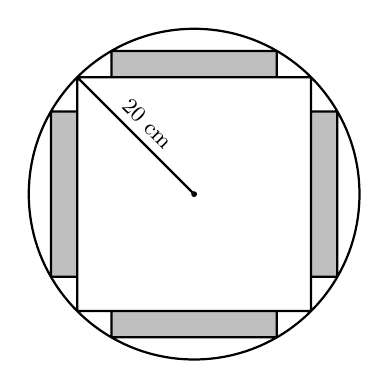
\begin{tikzpicture}[line join = round,line cap = round, >=stealth, thick, font = \small, scale = 0.7]
			\path
			(0,0) coordinate (O)
			+(45:3) coordinate (N)
			+(135:3) coordinate (M)
			+(-45:3) coordinate (P)
			+(-135:3) coordinate (Q)
			+(150:3) coordinate (A)
			+(30:3) coordinate (B)
			+(-30:3) coordinate (C)
			+(-150:3) coordinate (D)
			+(60:3) coordinate (F)
			+(120:3) coordinate (E)
			+(-60:3) coordinate (G)
			+(-120:3) coordinate (H)
			(intersection of A--B and M--Q) coordinate (1)
			(intersection of A--B and N--P) coordinate (2)
			(intersection of C--D and M--Q) coordinate (4)
			(intersection of C--D and N--P) coordinate (3)
			(intersection of E--H and M--N) coordinate (5)
			(intersection of F--G and M--N) coordinate (6)
			(intersection of F--G and P--Q) coordinate (7)
			(intersection of E--H and Q--P) coordinate (8)
			;
			\fill[gray!50]
			(E)--(F)--(6)--(5)--cycle
			(2)--(B)--(C)--(3)--cycle
			(7)--(G)--(H)--(8)--cycle
			(1)--(A)--(D)--(4)--cycle
			;
			\draw (O) circle (3)
			(M)--(N)--(P)--(Q)--cycle
			(D)--(A)--(1)
			(C)--(B)--(2)
			(C)--(3)
			(D)--(4)
			(5)--(E)--(F)--(6)
			(7)--(G)--(H)--(8)
			(1)--(A)--(D)--(4)
			(O)--(M) node[midway, sloped,above]{$20$ cm}
			;
			\foreach \x/\g in {O/90}\fill (\x) circle (1.5pt)+(\g:3mm) node{};
		\end{tikzpicture}
	\end{center}
	\shortans{67,3}
	\loigiai{
		\begin{center}
			\begin{tikzpicture}[line join = round,line cap = round, >=stealth, thick, font = \small, scale = 0.7]
				\path
				(0,0) coordinate (O)
				+(45:3) coordinate (N)
				+(135:3) coordinate (M)
				+(-45:3) coordinate (P)
				+(-135:3) coordinate (Q)
				+(150:3) coordinate (A)
				+(30:3) coordinate (B)
				+(-30:3) coordinate (C)
				+(-150:3) coordinate (D)
				+(60:3) coordinate (F)
				+(120:3) coordinate (E)
				+(-60:3) coordinate (G)
				+(-120:3) coordinate (H)
				(intersection of A--B and M--Q) coordinate (1)
				(intersection of A--B and N--P) coordinate (2)
				(intersection of C--D and M--Q) coordinate (4)
				(intersection of C--D and N--P) coordinate (3)
				(intersection of E--H and M--N) coordinate (5)
				(intersection of F--G and M--N) coordinate (6)
				(intersection of F--G and P--Q) coordinate (7)
				(intersection of E--H and Q--P) coordinate (8)
				;
				\fill[gray!50]
				(E)--(F)--(6)--(5)--cycle
				(2)--(B)--(C)--(3)--cycle
				(7)--(G)--(H)--(8)--cycle
				(1)--(A)--(D)--(4)--cycle
				;
				\draw (O) circle (3)
				(M)--(N)--(P)--(Q)--cycle
				(D)--(A)--(1)
				(C)--(B)--(2)
				(C)--(3)
				(D)--(4)
				(5)--(E)--(F)--(6)
				(7)--(G)--(H)--(8)
				(1)--(A)--(D)--(4)
				;
				\foreach \x/\g in {O/90}\draw[fill=black] (\x) circle (1.5pt)+(\g:3mm) node{};
				\path ($(E)!0.5!(F)$) coordinate (9)
				($(M)!0.5!(N)$) coordinate (10);
				\draw[fill=black] (5) circle (1pt)  node[below]{$A$}
				(6) circle (1.2pt) node[below]{$B$}
				(F) circle (1.2pt) node[above right]{$C$}
				(E) circle (1.2pt) node[above left]{$D$}
				(9) circle (1.2pt) node[above]{\tiny $N$}
				(10) circle (1.2pt) node[below left]{$M$};
				\draw (F)--(O)--(9); 
			\end{tikzpicture}
		\end{center}
		Gọi mặt cắt ngang của tấm ván là hình chữ nhật $ABCD$, $M$, $N$ lần lượt là trung điểm của $AB$, $CD$.\\
		Đặt $MN=x$, $OM=\dfrac{1}{2}\cdot 19\sqrt{2}=10\sqrt{2}$,  $ON=x+10\sqrt{2}$. Suy ra $$NC=\sqrt{O{C^2}-O{N^2}}=\sqrt{20^2-\left(x+10\sqrt{2}\right)^2}=\sqrt{-x^2-20\sqrt{2}x+200}.$$
		Kéo theo $AB=2\sqrt{-x^2-20\sqrt{2}x+200}$,
		$0<x<20-10\sqrt{2}$.\\
		Diện tích mặt cắt ngang của tấm ván là
		$$S=AB\cdot CD=2x\sqrt{-x^2-20\sqrt{2}x+200}=2\sqrt{-x^4-20\sqrt{2}{x^3}+200x^2}.$$
		Đặt $f(x)=-x^4-20\sqrt{x^3}+200x^2$, $0<x<20-10\sqrt{2}$. Khi đó
		\[f'(x)=0 \Leftrightarrow \heva{&-4x^3-60\sqrt{2}x^2+400x=0\\ &0<x<20-10\sqrt{2}} \Leftrightarrow x=\dfrac{5\sqrt{34}-15\sqrt{2}}{2}.\]
		Đặt $x_0=\dfrac{5\sqrt{34}-15\sqrt{2}}{2}$. Ta có bảng biến thiên
		\begin{center}
			
\begin{tikzpicture}[line join=round,font=\footnotesize,>=stealth, scale=1]
				\tkzTabInit[nocadre=false,lgt=1.2,espcl=2.5,deltacl=0.8]
				{$x$ /1,$f'$ /0.6,$f$ /2}
				{$0$, $x_0$, $20-10\sqrt{2}$}
				\tkzTabLine{,+,0,-,}
				\tkzTabVar{-/ ,+/ , -/ }
			\end{tikzpicture}
		\end{center}
		Suy ra $\max f(x) =f(x_0)$, do đó $\max S(x)=2\sqrt{f(x_0)}\approx 67{,}3$.
	}
\end{ex}

% #27 | Archive/SP_SauLuoi_2024-2025/SP_HKI/2-TN-DS-TLN-SGD-VinhLong-HKI-NH24-25.tex | mã gốc 2D1V1-1
\begin{ex}%[2D1V1-1]%[Dự án đề kiểm tra Khối 12 HK1 NH24-25 - Đợt 5 - Nguyễn Trần Anh Tuấn]%[SGD - Tỉnh Vĩnh Long]
	Một chất điểm chuyển động có phương trình $s(t)$ thì có vận tốc $v(t)=s'(t)$. Biết rằng phương trình chuyển động của chất điểm là $s(t)=\dfrac{1}{3}t^3-3t^2+5t$ trong đó $t$ được tính bằng giây và $s$ được tính bằng mét. Kể từ giây thứ bao nhiêu trở đi thì vận tốc của chất điểm bắt đầu tăng?
	\shortans{3}
	\loigiai{
		Ta có $v(t)=s'(t)=t^2-6t+5$, $t \ge 0$, suy ra $v'(t)=2t-6$.\\
		Lại có $v'(t)=0 \Leftrightarrow t=3$.\\
		Bảng biến thiên
		\begin{center}
			
\begin{tikzpicture}[line join=round,font=\footnotesize,>=stealth, scale=1]
				\tkzTabInit[nocadre=false,lgt=1.2,espcl=2.5,deltacl=0.8]
				{$x$ /1,$v'$ /0.6,$v$ /2}
				{$0$, $3$, $+ \infty$}
				\tkzTabLine{,-,0,+,}
				\tkzTabVar{+/$+ \infty$ ,-/$-4$, +/$+ \infty$}
			\end{tikzpicture}
		\end{center}
		Kể từ giây thứ $3$ trở đi thì vận tốc của chất điểm bắt đầu tăng.
	}
\end{ex}

% #35 | Archive/SP_SauLuoi_2024-2025/SP_HKI/2-TN-DS-TLN-THPT-PhaHuyChu-HaNoi-HKI-NH24-25.tex | mã gốc 2D1V3-6
\begin{ex}%[2D1V3-6]%[2-TN-DS-TLN-Phan Huy Chú-Hà Nội-HKI-24-25]%[Dương Đức]
	Sau khi phát hiện một dịch bệnh, các chuyên gia y tế ước tính số người nhiễm bệnh kể từ ngày phát hiện bệnh nhân đầu tiên đến ngày thứ $t$ là $f(t)=-\dfrac{t^3}{3}+17t^2+580t$, $t\in \mathbb{N}^*$, $t\leq 30$. Nếu coi $f(t)$ là hàm số xác định trên đoạn $[0;30]$ thì $f'(t)$ được xem là tốc độ truyền bệnh (người/ngày) tại thời điểm $t$. Trong $30$ ngày đầu tiên, ngày thứ bao nhiêu tốc độ truyền bệnh là lớn nhất?
	\shortans{$17$}	
	\loigiai{
		Xét hàm số $g(t)=f'(t)=-t^2+34t+580$ với $t\in [0;30]$.\\
		Khi đó $g'(t)=-2t+34$. Xét $g'(t)=0\Leftrightarrow t=17$.\\
		Bảng biến thiên 
		\begin{center}
			
\begin{tikzpicture}[>=stealth]
				\tkzTabInit[nocadre,lgt=1.5,espcl=3,deltacl=0.5]{$t$/.7,$g'(t)$/.7,$g(t)$/2.1}
				{$0$ ,  $17$ , $30$}
				\tkzTabLine{ , + , 0 , - }
				\tkzTabVar{-/$580$ , +/$869$ , -/$700$}
			\end{tikzpicture}
		\end{center}
		Do đó trong $30$ ngày đầu tiên, ngày thứ $17$ có tốc độ truyền bệnh là lớn nhất.	 
	}
\end{ex}

% #36 | Archive/SP_SauLuoi_2024-2025/SP_HKI/2-TN-DS-TLN-THPT-PhaHuyChu-HaNoi-HKI-NH24-25.tex | mã gốc 2D1V3-6
\begin{ex}%[2D1V3-6]%[2-TN-DS-TLN-Phan Huy Chú-Hà Nội-HKI-24-25]%[Dương Đức]
	Bộ phận sản xuất của một công ty xác định chi phí để sản xuất $x$ sản phẩm được cho bởi biểu thức $T(x)=x^2-20x+400$ (nghìn đồng). Nếu $x$ sản phẩm đều được bán hết và giá bán mỗi sản phẩm là $100$ nghìn đồng thì lợi nhuận lớn nhất mà công ty thu được là bao nhiêu nghìn đồng?
	\shortans{$3200$}
	\loigiai{
		Lợi nhuận của công ty thu được khi bán hết $x$ sản phẩm là $$f(x)=100x-T(x)=100x-x^2+20x-400=-x^2+120x-400 \textrm{~(nghìn đồng)}.$$
		Xét hàm số $y=f(x)$ với $x\in[0;+\infty)$.\\
		Ta có $y'=-2x+120$. Xét $y'=0\Leftrightarrow x=60$.\\
		Bảng biến thiên 
		\begin{center}
			
\begin{tikzpicture}[>=stealth]
				\tkzTabInit[nocadre,lgt=1.2,espcl=3,deltacl=0.6]{$x$/.7,$y'$/.7,$y$/2.1}
				{$0$ ,  $60$ , $+\infty$}
				\tkzTabLine{ , + , 0 , - }
				\tkzTabVar{-/$-400$ , +/$3200$ , -/$-\infty$}
			\end{tikzpicture}
		\end{center}
		Dựa vào bảng biến thiên suy ra lợi nhuận lớn nhất mà công ty thu được là $3200$ nghìn đồng.
	}
\end{ex}

% #41 | Archive/SP_SauLuoi_2024-2025/SP_HKI/2-TN-DS-TL-SGD-HUE-HKI-N24-25.tex | mã gốc 2D1H3-6
\begin{ex}%[2D1H3-6]%[Dự án đề kiểm tra Toán khối 12 HK1 NH23-24 đợt 5-Hoàng Thanh Phương]%[SGD Huế]
	Một chất điểm chuyển động trên đường thẳng có quãng đường đi được $s$ (tính bằng mét) theo thời gian $t$ (tính bằng giây) được biểu thị bởi công thức $s(t)=4t-\ln(1+t)$, $t\geq 0$.
	\choiceTF
	{Sau 5 giây, quãng đường di chuyển của chất điểm là $s=20$ (mét)}
	{Vận tốc tức thời tại thời điểm $t$ của chất điểm là $v(t)=1+s'(t)$}
	{\True Vận tốc tức thời tại thời điểm $t=2$ giây là $v(2)=\dfrac{11}{3}$ (m/s)}
	{Vận tốc luôn giảm theo thời gian}
	\loigiai{
		\begin{itemchoice}
			\itemch Ta có $s(5)=20-\ln 6$.
			\itemch Ta có $v(t)=s'(t)=4-\dfrac{1}{1+t}$.
			\itemch Vận tốc tức thời tại thời điểm $t=2$ là $v(2)=4-\dfrac{1}{1+2}=\dfrac{11}{3}$ (m/s).
			\itemch Ta có $v'(t)=\dfrac{1}{(1+t)^2}>0,~\forall t>0$. Vậy hàm $v(t)$ là hàm đồng biến trên $(0;+\infty)$ nên vận tốc của chất điểm tăng theo thời gian.
		\end{itemchoice}
	}
\end{ex}

% #52 | Archive/SP_SauLuoi_2024-2025/SP_HKI/2-TN-DS-TLN-TL-THPT-TranPhu-VungTau-HKI-NH24-25.tex | mã gốc 2D1V3-6
\begin{ex}%[2D1V3-6]%[2-TN-DS-TLN-THPT-TranPhu-VungTau-HKI-NH24-25]%[Hiếu Mai]
Một vận động viên thể thao hai môn phối hợp luyện tập với một bể bơi hình chữ nhật rộng $400$ m, dài $800$ m. Vận động viên chạy phối hợp với bơi như sau: Xuất phát từ điểm $A$, chạy đến điểm $X$ và bơi từ điểm $X$ đến điểm $C$ (Hình).
\begin{center}
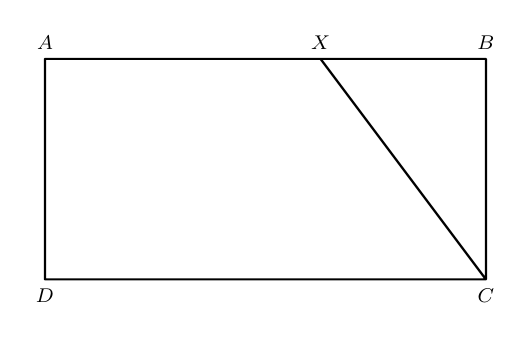
\begin{tikzpicture}[
	>=stealth, line join=round, line cap=round, 
	scale=.7,
	font=\footnotesize,
	declare function={r=3; a=75;}]
	\draw[thick]
		(0,0) node[below] {$D$} --
		(0,4) node[above] {$A$} --
		(5,4) node[above] {$X$} -- 
		(8,4) node[above] {$B$} --
		(8,0) node[below] {$C$} --
		(0,0) -- cycle
		(5,4) -- (8,0)
		;
\end{tikzpicture}
\end{center}
Hỏi nên chọn điểm $X$ cách $A$ gần bằng bao nhiêu mét để vận động viên đến $C$ nhanh nhất (làm tròn kết quả đến hàng đơn vị)? Biết rằng vận tốc chạy là $30$ km/h, vận tốc bơi là $6$ km/h.
\shortans{$718$}
\loigiai{
Gọi $x$ m là khoảng cách từ $A$ đến $X$ (0<x<800). Khi đó
\begin{align*}
	XB &= (800-x)\,\text{m} \\
	XC &= \sqrt{(800-x)^2+400^2}\,\text{m} \\
	&= \sqrt{x^2-1600x+800\,000}\,\text{m}.
\end{align*}
Thời gian để vận động viên hoàn thành việc chạy và bơi là
$$
	t = \dfrac{1}{1000}\left(\dfrac{x}{30} + \dfrac{\sqrt{x^2-1600x+800\,000}}{6}\right) \,\text{h}.
$$
Đặt $f(x) = \dfrac{x}{5}+\sqrt{x^2-1600x+800\,000}$. Ta thấy $f(x)$ xác định trên $\mathbb{R}$ và có đạo hàm
$$
	f'(x) = \dfrac{1}{5}+\dfrac{x-800}{\sqrt{x^2-1600x+800\,000}}.
$$
Cho $f'(x)=0$ rồi giải ra, ta được $x=882$ hoặc $x \approx 718$.\\
Ta thấy
\begin{align*}
	f(0) &\approx 894 \\
	f(718) &\approx 552 \\
	f(800) &= 560.
\end{align*}
Do vậy, để thời gian hoàn thành bài thi ngắn nhất thì vận động viên nên chọn vị trí $X$ cách $A$ $718$ mét.
}
\end{ex}

% #62 | Archive/SP_SauLuoi_2024-2025/SP_HKI/2-TN-DS-TLN-THPT-NguyenKhuyen-AnGiang-HKI-NH24-25.tex | mã gốc 2D1H3-6
\begin{ex}%[2D1H3-6]%[Dự án đề kiểm tra Toán 12 HKI NH24-25- Lê Hồ Quang Minh]%[THPT Nguyễn Khuyến - An Giang]
	Hằng ngày mực nước của hồ thủy điện ở miền Trung lên và xuống theo lượng nước mưa và các suối nước đổ về hồ. Từ lúc 8h giờ sáng, độ sâu của mực nước trong hồ tính theo mét và lên xuống theo thời gian $t$ (giờ) trong ngày cho bởi công thức $h\left(t\right)=24t+5t^2-\dfrac{t^3}{3}$. Biết rằng phải thông báo cho các hộ dân di dời trước khi xả nước theo quy định trước $5$ giờ. Hỏi cần thông báo cho hộ dân di dời trước khi xả nước mấy giờ? Biết rằng mực nước trong hồ phải lên cao nhất mới xả nước.
	\shortans{15}
	\loigiai{
		Xét hàm số $h\left(t\right)=24t+5t^2-\dfrac{t^3}{3}$, $t \in \left[8;24\right]$.\\
		Ta có ${h}'\left(t\right)=24+10t-t^2$.\\
		${h}'\left(t\right)=0 \Leftrightarrow 24+10t-t^2=0 \Leftrightarrow \hoac{&t=-2\\ &t=12}$\\
		Khi đó: $h\left(8\right)=\dfrac{1024}{3}$, $h\left(12\right)=432$, $h\left(24\right)=-1152$.\\
		Suy ra: $\max\limits_{\left[8;24\right]} h\left(t\right)=432$ khi $t=12$.\\
		Tức là: đến $20$ cùng ngày thì mực nước trong hồ sẽ lên cao nhất. Mà theo quy định phải báo trước $5$ giờ nên cần thông báo cho hộ dân di dời trước khi xả nước vào lúc $15$ giờ chiều.
	}
\end{ex}

% #65 | Archive/SP_SauLuoi_2024-2025/SP_HKI/2-TN-DS-TLN-THPT-NguyenKhuyen-AnGiang-HKI-NH24-25.tex | mã gốc 2D1C5-8
\begin{ex}%[Đề thi HK1 lớp 12 THPT Nguyễn Khuyến-An Giang NH 24-25]%[Nguyễn Tấn Linh]%[2D1C5-8]
	\immini
	{
		Một miếng nhôm có bề ngang 30 cm được uốn cong tạo thành máng dẫn nước bằng cách chia tấm nhôm thành 3 phần bằng nhau rồi gấp 2 bên lại theo một góc $\theta \left(0<\theta \le \dfrac{\pi}{2}\right)$ như hình vẽ dưới. Hỏi $\theta$ bằng bao nhiêu để tạo ra máng có diện tích mặt ngang $S$ lớn nhất để có thể cho nước đi qua nhiều nhất? ($\theta$ tính theo radian và làm tròn đến hàng phần trăm).\shortans{$1,05$}
	}
	{
		\begin{tikzpicture}[line join = round, line cap = round,>=stealth,font=\footnotesize,scale=1]
			\def \canh{2}
			\def \goc{60}
			\draw (0,0) coordinate(O)--(\canh,0) coordinate(A)--++(\canh,0) coordinate(B)--++(\canh,0) coordinate(C);
			\draw[thick] (A)--(B) (B)--++(\goc:\canh) coordinate(D) (A)--++({180-\goc}:\canh) coordinate(E);
			\path[->] pic[angle radius=3mm,draw,"$\theta$",angle eccentricity=1.5] {angle = C--B--D};
			\path[<-] pic[angle radius=3mm,draw,"$\theta$",angle eccentricity=1.5] {angle = E--A--O};
			\foreach \i in {0,1,2}\draw[<->] (\i*\canh,-0.3)--++(\canh,0) node[midway,fill=white]{$10$ cm};
		\end{tikzpicture}
	}
	\loigiai
	{
		Đặt các điểm $A$, $B$, $C$, $D$, $H$ (với $H$ là hình chiếu của $B$ lên $AD$) như hình vẽ
		\begin{center}\begin{tikzpicture}[line join = round, line cap = round,>=stealth,font=\footnotesize,scale=1]
				\def \canh{2}
				\def \goc{60}
				\draw (0,0) coordinate(O)
				-- (\canh,0) coordinate(B)
				-- ++(\canh,0) coordinate(C)
				-- ++(\canh,0) coordinate(X);
				\draw[thick]
				(B)--(C)
				(C)-- ++(\goc:\canh) coordinate(D)
				(B)-- ++({180-\goc}:\canh) coordinate(A);
				\path[->] pic[angle radius=3mm,draw,"$\theta$",angle eccentricity=1.5]
				{angle = X--C--D};
				\path[<-] pic[angle radius=3mm,draw,"$\theta$",angle eccentricity=1.5]
				{angle = A--B--O};
				\foreach \i in {0,1,2}{
					\draw[<->] (\i*\canh,-0.5)--++(\canh,0)
					node[midway,fill=white]{$10$ cm};
				}
				\coordinate (H) at ($(A)!(B)!(D)$);
				\draw (A)--(D) (B)--(H);
				\foreach \diem/\goc in {A/90,H/90,D/90,B/-90,C/-90} \fill[black](\diem) circle (1pt) ($(\diem)+(\goc:3mm)$) node{$\diem$};
		\end{tikzpicture}\end{center}
		$\Rightarrow BC=AB=CD=10$; $BH=AB\cdot\sin \theta =10\cdot\sin \theta$; $AD=BC+2AH=10+20\cdot\cos \theta $.\\
		Lúc này diện tích mặt ngang $S$ chính là diện tích hình thang cân $ABCD$
		\allowdisplaybreaks
		\begin{eqnarray*}
			S_{ABCD}&=&\dfrac{1}{2}\cdot BH\cdot \left(AD+BC\right)=\dfrac{1}{2}\cdot 10\cdot \sin \theta \cdot \left(10+20\cdot \cos \theta +10\right)\\
			&=&10\cdot \sin \theta \cdot \left(10+10\cdot \cos \theta\right)\\
			\Rightarrow {S_{ABCD}}&=&100\cdot \left(\sin \theta +\sin \theta\cdot \cos \theta\right)\\
			&=&100\cdot \left(\sin \theta +\sin \theta\cdot \sqrt{1-\sin^2\theta}\right)\text{ do }\left(0<\theta \le \dfrac{\pi}{2}\right).
		\end{eqnarray*}
		Đặt $t=\sin \theta,\,t\in \left(0;1\right]$ do $\left(0<\theta \le \dfrac{\pi}{2}\right)$.\\
		Xét hàm số $f\left(t\right)=100\left(t+t\sqrt{1-t^2}\right)$ với $t\in \left(0;1\right]$
		$$\begin{aligned}
			& \Rightarrow f'\left(t\right)=100\left(1+\sqrt{1-t^2}-\dfrac{t^2}{\sqrt{1-t^2}}\right)=0 \\
			& \Leftrightarrow 1=\dfrac{t^2}{\sqrt{1-t^2}}-\sqrt{1-t^2} \\
			& \Leftrightarrow{1^2}=\left(\dfrac{t^2}{\sqrt{1-t^2}}-\sqrt{1-t^2}\right)^2 \\
			& \Leftrightarrow 1=\dfrac{t^4}{1-t^2}+1-t^2-2t^2 \\
			& \Leftrightarrow 1-t^2=t^4+\left(1-3t^2\right)\left(1-t^2\right) \\
			& \Leftrightarrow 4t^4-3t^2=0 \\
			& \Leftrightarrow \hoac{&t^2=0\Rightarrow t=0&&(\text{loại}) \\&t^2=\dfrac{3}{4}\Rightarrow t=\dfrac{\sqrt{3}}{2}&&(\text{nhận}).} \\
		\end{aligned}$$
		Bảng biến thiên
		\begin{center}
			
\begin{tikzpicture}
				\tkzTabInit[
				lgt=1.5, % chiều dài của cột
				espcl=2,deltacl=0.8
				]{$t$ /1, $f'(t)$ /1, $f(t)$ /2}{$0$, $\frac{\sqrt{3}}{2}$, $1$}
				\tkzTabLine{,+,0,-,}
				\tkzTabVar{-/, +/ $75\sqrt{3}$, -/}
			\end{tikzpicture}
		\end{center}
		$\Rightarrow \max\limits_{\left[0;1\right]}f\left(t\right)=f\left(\dfrac{\sqrt{3}}{2}\right)=75\sqrt{3}$.\\
		Do đó, $S_{ABCD}$ lớn nhất là $75\sqrt{3}$ (cm$^2$) khi $\sin \theta =\dfrac{\sqrt{3}}{2}\Rightarrow \theta =\dfrac{\pi}{3}\approx 1{,}05$.
	}
\end{ex}

% #67 | Archive/SP_SauLuoi_2024-2025/SP_HKI/2-TN-DS-TLN-THPT-MarieCurie-HCM-HKI-NH24-25.tex | mã gốc 2D1H3-6
\begin{ex}%[2D1H3-6]%[Dự án A - HKI - THPT Marie Curie - TP. Hồ Chí Minh - 24-25]%[Nguyễn Ngọc Huy Trường]
	Một nhà sản xuất Robot xác định rằng để bán được $x$ đơn vị Robot, giá bán mỗi đơn vị (triệu đồng) phải là $p(x) = 1\,000-x$. Nhà sản xuất cũng xác định rằng tổng chi phí sản xuất $x$ đơn vị được cho bởi $C(x) = 3\,000 + 20x$. Khi đó
	\choiceTF
	{Tổng doanh thu $R(x) = x+p(x)$}
	{\True Tổng lợi nhuận $P(x) = R(x) - C(x)$}
	{\True Để tối đa hóa lợi nhuận thì công ty phải sản xuất và bán $490$ đơn vị Robot}
	{\True Giá bán mỗi đơn vị là $510$ (triệu đồng) thì công ty đạt được lợi nhuận tối đa}
	\loigiai{
		\begin{itemchoice}
			\itemch \textbf{Sai}. Tổng doanh thu $R(x) = xp(x) = x(1\,000-x) = 1000x - x^2$. 
			\itemch \textbf{Đúng}. Tổng lợi nhuận $P(x) = R(x) - C(x)$.
			\itemch \textbf{Đúng}. Ta có $P(x) = R(x) - C(x) = 1\,000x - x^2 - (3\,000+20x) = -x^2 + 980x - 3\,000$. \\
			Suy ra $P'(x) = -2x + 980$. Khi đó $P'(x) = 0 \Leftrightarrow -2x + 980 = 0 \Leftrightarrow x = 490$. \\
			Ta có bảng biến thiên của $P(x)$ như sau
			\begin{center}
				
\begin{tikzpicture}
					\tkzTabInit[nocadre=false,lgt=1.3,espcl=2.5,deltacl=0.7]
					{$x$/0.7,$P'(x)$/0.7,$P(x)$/1.5}
					{$0$,$490$,$+\infty$}
					\tkzTabLine{,+,0,-,}   
					\tkzTabVar{-/$-3\,000$,+/$237\,100$,-/$-\infty$}
				\end{tikzpicture}
			\end{center}
			Vậy để tối đa hoá lợi nhuận thì công ty phải sản xuất và bán $490$ đơn vị Robot.
			\itemch \textbf{Đúng}. Khi $x = 490$ thì $p(490) = 1\,000 - 490 = 510$. \\
			Vậy giá bán mỗi đơn vị là $510$ (triệu đồng) thì công ty đạt được lợi nhuận tối đa
		\end{itemchoice}
	}
\end{ex}

% #74 | Archive/SP_SauLuoi_2024-2025/SP_HKI/2-TN-DS-TLN-THPT-MarieCurie-HCM-HKI-NH24-25.tex | mã gốc 2D1V3-3
\begin{ex}%[2D1V3-3]%[Dự án đề kiểm tra Toán 12 GHKI NH23-24- Trần Xuân Hòa]%[THPT MarieCurie - Tp HCM]
Một con đường cần được xây dựng giữa hai thành phố $X$ và $Y$ nằm ở hai bên đối diện của một con sông có chiều rộng đều  bằng $1$ km. Thành phố $X$ cách sông $2$ km và $Y$ cách sông $4$ km, khoảng cách giữa hai hình chiếu vuông góc của $X$ và $Y$ trên bờ sông là $X'Y'=6$ km. Một cây cầu sẽ được xây dưng để cho phép giao thông đi qua sông. Vị trí của cây cầu $CD$ cách $XX'$ là $x$ (km). Tìm $x$ để con đường cần được xây dựng giữa hai thành phố $X$ và $Y$ được ngắn nhất.
\shortans{$2$}
\begin{center}
	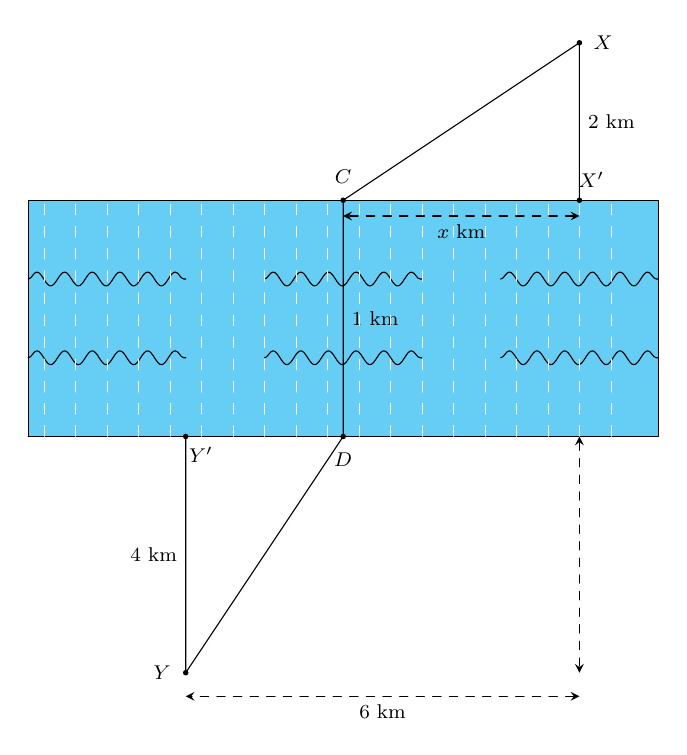
\begin{tikzpicture}[scale=1, font=\footnotesize,line join=round, line cap=round, >=stealth]
		\def\a{8} %%chiều dài
		\def\b{3} %%chiều rộng
		\path 
		(0,0) coordinate (A)
		(\a,0) coordinate (B)
		(8,3) coordinate (K)
		(7,5) coordinate (X)
		(7,3) coordinate (X')
		(2,-3) coordinate (Y)
		(2,0) coordinate (Y')
		(4,0) coordinate (D)
		(4,3) coordinate (C)
		;
		\draw [fill=cyan!60](A)--(B)--(K)--(0,3)--(A);
		\draw (X')--(X)--(C)--(D)--(Y)--(Y');
		\draw (X)--(X')node[right,midway]{$2$ km};
		\draw (Y)--(Y')node[left,midway]{$4$ km};
		\draw (D)--(C)node[right,midway]{$1$ km};
		\draw[dashed,<->] (7,-3.3)--(2,-3.3)node[midway,below]{$6$ km};
		\draw[dashed,<->] (7,2.8)--(4,2.8)node[midway,below]{$x$ km};
		\draw[dashed,<->] (7,0)--(7,-3);
		\foreach \i/\g in {C/90,D/-90,X/0,Y/180,X'/60,Y'/-50}
		\fill[black] (\i) circle(1pt)+(\g:3mm)node[scale=1]{$\i$};
		\draw[decorate,decoration=snake] (0,1) - - (2,1) ;
		\draw[decorate,decoration=snake] (0,2) - - (2,2) ;
		\draw[decorate,decoration=snake] (3,1) - - (5,1) ;
		\draw[decorate,decoration=snake] (3,2) - - (5,2) ;
		\draw[decorate,decoration=snake] (6,1) - - (8,1) ;
		\draw[decorate,decoration=snake] (6,2) - - (8,2) ;
		\foreach \i in {0.2,0.6,...,7.8}
		\draw[ultra thin,white,dash pattern=on 4pt off 4pt] (\i,0)--(\i,3);
	\end{tikzpicture}
\end{center}	
	\loigiai{Theo giả thiết ta có $XX'=2$, $YY'=4$, $CD=1$.\\
	Ta tính được $CX=\sqrt{x^2+4}$, $DY=\sqrt{4^2+(6-x)^2}$.\\
	Quãng đường hai thành phố có độ dài là 
	\[f(x)=XC+CD+DY=1+\sqrt{x^2+4}+\sqrt{x^2-12x+52}.\]
	Tìm giá trị nhỏ nhất của $f(x)$.
	\begin{itemize}
		\item Cách 1: Sử dụng CASIO.
		\item Cách 2: Sử dụng Bất đẳng thức $\sqrt{a_1^2+b_1^2}+\sqrt{a_2^2+b_2^2}\ge \sqrt{(a_1+a_2)^2+(b_1+b_2)^2}$.\\
		Dấu bằng đạt được khi và chỉ khi $a_1b_2=a_2b_1$. Ta có
		 \begin{eqnarray*}
			&CX+DY&=\sqrt{x^2+2^2}+\sqrt{(6-x)^2+4^2}\\
			&&\ge \sqrt{(x+6-x)^2+(2+4)^2}\\
			&&=6\sqrt{2}.
		\end{eqnarray*}
		Dấu bằng xảy ra khi và chỉ khi $4x=2(6-x)\Leftrightarrow x=2$.\\
		Do đó quãng đường hai thành phố đạt giá trị nhỏ nhất khi $x=2$.
		\item Cách 3: Khảo sát hàm số. Ta có $f'(x)=\dfrac{x}{\sqrt{x^2+4}}+\dfrac{x-6}{x^2-12x+52}=0$ có nghiệm $x=2$ duy nhất trên $(0;6)$.
		\[\begin{aligned}
			f'(x)=0 & \Leftrightarrow \dfrac{x}{\sqrt{x^2+4}}=\dfrac{6-x}{\sqrt{x^2-12 x+52}} \\
			& \Leftrightarrow \dfrac{x^2}{x^2+4}=\dfrac{(6-x)^2}{x^2-12 x+52}, \quad(0<x<6) \\
			& \Leftrightarrow \dfrac{x^2}{x^2+4}-1=\dfrac{x^2-12 x+36}{x^2-12 x+52}-1 \\
			& \Leftrightarrow-\dfrac{4}{x^2+4}=-\dfrac{16}{x^2-12 x+52} \\
			& \Leftrightarrow x^2-12 x+52=4\left(x^2+4\right) \\
			& \Leftrightarrow 3 x^2+12 x-36=0 \\
			& \Leftrightarrow\hoac{&x=2\\&x=-6\text{ (Loại).}}
		\end{aligned}\]
	\end{itemize}
	}
\end{ex}

% #80 | Archive/SP_SauLuoi_2024-2025/SP_HKI/2-TN-DS-TLN-THPT-ThiXaQuangTri-QuangTri-HKI-NH24-25.tex | mã gốc 2D1V3-6
\begin{ex}%[2D1V3-6]%[Dự án đề kiểm tra Toán 12 HKI NH23-24- Xuan Vy Pham]%[THPT Thị Xã Quảng Trị]
\immini{Khi dạo chơi trên một công viên, bạn Đoàn di chuyển trên đường parabol, bạn Kết di chuyển trên đường tròn (xem hình vẽ bên). Khoảng cách giữa đỉnh $A$ của parabol và  tiếp điểm $B$ của đường tròn là $16$m, $HK \perp AB$ và $AH=6$m, $HK=9$m. Tìm khoảng cách nhỏ nhất giữa hai bạn Đoàn và Kết, biết rằng đường tròn có bán kính bằng $3$m (\textit{làm tròn đến hàng phần trăm}).}{\begin{tikzpicture}[line join=round, line cap=round,>=stealth,font=\footnotesize,scale=1]
		\def\x{3}
		\def\y{5}
		\def\z{3}
		\path (0:0) coordinate (H)
		++(0:\x) coordinate (B)
		(H)++(180:0.4*\x) coordinate (A)
		(H)++(90:\z) coordinate (K)
		(3,1)++(30:1) coordinate (E)
		(E)++(180:4.22) coordinate (F)
		;
		\draw[thick] (A)--(B) (H)--(K);
		\draw[smooth,blue,thick] plot[domain=-2.4:0](\x,{25/12*(\x)*(\x)+5*(\x)+3});
		\draw[smooth,red,thick] (3,1) circle (1);
		\foreach \x/\g in {A/-90,H/-90,B/-90,K/180}
		\fill[black] (\x) circle (1pt) ($(\g:4mm)+(\x)$) node {$\x$};	
		\draw(F) node[left]{Đoàn};
		\draw(E) node[above right]{Kết};
		\foreach \x/\g in {E/180,F/20}
		\fill[blue] (\x) circle (1.6pt) ($(\g:4mm)+(\x)$);	
\end{tikzpicture}}
\shortans{8,43}
\loigiai{
\begin{center}
\begin{tikzpicture}[line join=round, line cap=round,>=stealth,font=\footnotesize,scale=1]
		\def\x{3}
		\def\y{5}
		\def\z{3}
		\path (0:0) coordinate (H)
		++(0:\x) coordinate (B)
		(H)++(180:0.4*\x) coordinate (A)
		(H)++(90:\z) coordinate (K)
		(3,1)++(30:1) coordinate (E)
		(E)++(180:4.22) coordinate (F)
		(3,1) coordinate (I)
		;
		%Vẽ các trục
		\draw[->,thick] (H)--($(H)!1.5!(B)$) node[below]{$x$};
		\draw[->,thick] (H)--($(H)!1.2!(K)$) node[right]{$y$};
		\draw[thick] (A)--(B) (H)--(K);
		\draw[smooth,blue,thick] plot[domain=-2.4:0](\x,{25/12*(\x)*(\x)+5*(\x)+3});
		\draw[smooth,red,thick] (I) circle (1);
		\foreach \x/\g in {A/-90,H/-90,B/-90,K/180}
		\fill[black] (\x) circle (1pt) ($(\g:4mm)+(\x)$) node {$\x$};	
		\foreach \x/\g in {E/30,F/180,I/20}
		\fill[blue] (\x) circle (1.6pt) ($(\g:4mm)+(\x)$)  node {$\x$};		
\end{tikzpicture}
\end{center}
Chọn hệ trục tọa độ $Oxy$ với $O \equiv H$, $Ox$ trùng $HB$, $Oy$ trùng $HK$.\\
Ta có $HB=AB-AH=16-6=10$.\\
Từ giả thiết đề bài, ta được $H(0;0)$, $A(-6;0)$, $K(0;9)$, $B(10;0)$.\\
Giả sử vị trí của bạn Đoàn và bạn Kết trên hệ trục tọa độ lần lượt là hai điểm $F$ và $E$.\\
Gọi $I$ là tâm đường tròn mà bạn Kết di chuyển trên.\\
Vì $B(10;0)$ là hình chiếu của $I$ lên trục $Ox$ nên $I(10;y_I)$.\\
Mà bán kính đường tròn bằng $3$ nên $y_I=3$. Do đó $I(10;3)$.\\
Cố định điểm $F$ thuộc parabol. \\
Theo bất đẳng thức tam giác, ta có $FE \ge FI-IE = FI-3$.\\
Vậy $FE_\text{min}$ bằng $FI-3$.\\
Dấu "=" xảy ra khi và chỉ khi $F$, $E$, $I$ thẳng hàng và $E$ nằm giữa $F$ và $I$.
Bạn Đoàn di chuyển trên parabol $(P)$ là đồ thị của hàm số bậc hai có dạng $y=ax^2+bx+c$.\\
Vì $(P)$ đi qua điểm $A(-6;0)$, $K(0;9)$ và có hoành độ đỉnh bằng $-6$ nên
$$\heva{&(-6)^2a+(-6)b+c=0\\&0^2a+0b+c=9\\&\dfrac{-b}{2a}=-6} \Leftrightarrow \heva{&36a-6b+c=0\\&c=9\\&12a-b=0} \Leftrightarrow \heva{&a=\dfrac{1}{4}\\&b=3\\&c=9.}$$
Vậy $(P) \colon y =\dfrac{1}{4}x^2+3x+9$.\\
Vì điểm $F$ thuộc $(P)$ nên tọa độ của $F$ có dạng $F \left(x;\dfrac{1}{4}x^2+3x+9\right)$.\\
Ta có $EF=FI-3=\sqrt{(x-10)^2+\left(\dfrac{1}{4}x^2+3x+6\right)^2}-3$.\\
Đặt $f(x)=\sqrt{(x-10)^2+\left(\dfrac{1}{4}x^2+3x+6\right)^2}-3$.\\
Ta có $f'(x)=\dfrac{2(x-10)+2\left(\dfrac{1}{4}x^2+3x+6\right)\left(\dfrac{1}{2}x+3\right)}{2\sqrt{(x-10)^2+\left(\dfrac{1}{4}x^2+3x+6\right)^2}}=\dfrac{\dfrac{1}{8}x^3+\dfrac{9}{4}x^2+13x+8}{\sqrt{(x-10)^2+\left(\dfrac{1}{4}x^2+3x+6\right)^2}}$.
Cho $f'(x)=0 \Leftrightarrow x \approx -0{,}7$.\\
Bảng biến thiên
\begin{center}
	
\begin{tikzpicture}
		\tkzTabInit[lgt=1.2,espcl=2.3]
		{$x$ /0.8, $f’(x)$ /0.8, $f(x)$ /2}
		{$-\infty$,$-0{,}7$,$+\infty$}
		\tkzTabLine{ ,-,z,+, }
		\tkzTabVar{+/$+\infty$,-/$8{,}43$,+/$+\infty$}
	\end{tikzpicture}
\end{center}
Dựa vào bảng biến thiên, ta được giá trị nhỏ nhất của $f(x)$ trên $\mathbb{R}$ là $8{,}43$.\\
Vậy khoảng cách nhỏ nhất giữa hai bạn Đoàn và Kết là $8{,}43$m.
}
\end{ex}

% #91 | Archive/SP_SauLuoi_2024-2025/SP_HKI/2-TN-DS-TLN-THPT-ChuyenLeHongPhong-HCM-HKI-NH24-25.tex | mã gốc 2D1V3-6
\begin{bt}%[2D1V3-6]%[Dự án đề kiểm tra Toán 12 HKI Dot 04 NH24-25-Lê Hữu Kiệt]%[THPT Chuyên Lê Hồng Phong - TP Hồ Chí Minh]
	Một trang trại mỗi ngày thu hoạch được một tấn rau. Mỗi ngày, nếu bán rau với giá $30\,000$~đồng/kg thì hết sạch rau, ước chừng nếu giá bán tăng thêm $1\,000$ đồng/kg thì số rau thừa lại tăng thêm $20$ kg. Số rau thừa này được thu mua làm thức ăn chăn nuôi với giá $2\,000$ đồng/kg. Hỏi trang trại bán rau với giá bao nhiêu nghìn đồng mỗi kg thì có thể thu được nhiều tiền nhất?
	\par\shortans{$41$}
	\loigiai{
	$1$ tấn $=1\,000$ kg.\\
	Gọi $x$ (nghìn đồng) là số tiền tăng thêm trên mỗi kg rau ($x\geq 0$).\\
	Số tiền trang trại thu được (đơn vị: nghìn đồng) sau khi tăng $x$ nghìn đồng là
	\begin{eqnarray*}
		&T(x) &= (30+x)(1\,000-20x) + 20x\cdot 2 \\
		&&= -20x^2+440x+30\,000.
	\end{eqnarray*}
	Ta có $T'(x)=-40x+440$. Cho $T'(x)=0 \Leftrightarrow -40x+440=0 \Leftrightarrow x=11$.\\
	Bảng biến thiên
	\begin{center}
	
\begin{tikzpicture}[font=\footnotesize, >=stealth]
	\tkzTabInit[lgt=1.2,espcl=2.5,deltacl=0.6]
		{$x$/0.7, $T'(x)$/0.7, $T(x)$/2}
		{$0$, $11$ , $50$}
	\tkzTabLine
		{, + , $0$ , - , }
	\tkzTabVar
		{-/$30\,000$, +/$32\,420$, -/$2\,000$}
	\end{tikzpicture}
	\end{center}
	Từ bảng biến thiên suy ra, để có thể thu được nhiều tiền nhất, trang trại bán rau nên tăng $11$ nghìn đồng.\\
	Vậy giá bán một kg rau là $30+11\cdot 1=41$ nghìn đồng.
	}
\end{bt}

% #92 | Archive/SP_SauLuoi_2024-2025/SP_HKI/2-TN-DS-TLN-THPT-DinhTienHoang-NinhBinh-HKI-NH24-25.tex | mã gốc 2D1H3-6
\begin{ex}%[2D1H3-6]%[Dự án đề kiểm tra Khối 12 HK1 NH24-25 - Đợt 4 - Quang Vinh NT]%[THPT Đinh Tiên Hoàng - Tỉnh Ninh Bình]
	Một vật chuyển động theo quy luật $s(t) = t^3 - 3t^2 + 9t + 36$, với $t$ (giây) là khoảng thời gian tính từ lúc chất điểm bắt đầu chuyển động và $s$ là quãng đường vật đi được trong khoảng thời gian đó, tính bằng mét $(m)$.  
	\choiceTF
	{Quãng đường vật đi được sau $4$ giây kể từ lúc bắt đầu chuyển động là $82$ m}
	{\True Vận tốc của vật tại giây thứ $t$ là $v(t) = 3t^2 - 6t + 9$}
	{Gia tốc của vật tại thời điểm $2$ giây là $4$ $(m/s^2)$}
	{\True Trong khoảng thời gian $10$ (s) đầu tiên, vận tốc của vật nhỏ nhất là $6$ $(m/s)$}
	\loigiai{
		\begin{itemchoice}
			\itemch \textbf{Quãng đường sau $4$ giây:}  
			$$
			s(4) = 4^3 - 3 \cdot 4^2 + 9 \cdot 4 + 36 = 88 \, \text{m}.
			$$
			\itemch \textbf{Vận tốc tại giây thứ $t$:}  
			$$
			v(t) = s'(t) = 3t^2 - 6t + 9.
			$$			
			\itemch \textbf{Gia tốc tại thời điểm $t = 2$:}  
			Gia tốc là đạo hàm bậc hai của $s(t)$, tức là:
			$$
			a(t) = v'(t) =  6t - 6.
			$$
			Tại $t = 2$:
			$$
			a(2) = 6 \cdot 2 - 6 = 12 - 6 = 6 \, \text{m/s}^2.
			$$
			
			\itemch \textbf{Vận tốc nhỏ nhất trong $10$ giây đầu tiên:}  
			Xét hàm vận tốc $v(t) = 3t^2 - 6t + 9$.  
			Đạo hàm của $v(t)$:
			$$
			v'(t) = 6t - 6.
			$$
			Phương trình $v'(t) = 0\Leftrightarrow 			6t - 6 = 0  \Leftrightarrow  t = 1.
			$\\
			Bảng biến thiên 
			\begin{center}
				
\begin{tikzpicture}
					\tkzTabInit[lgt=1.5,espcl=2]
					{$t$/1, $v'(t)$/1, $v(t)$/2}
					{$0$, $1$, $10$}
					\tkzTabLine{,+,0,-,}
					\tkzTabVar{+/ $9$, -/ $6$, +/ $249$}
				\end{tikzpicture}
			\end{center}	
			Giá trị nhỏ nhất của $v(t)$ trên $[0; 10]$ là $v(1) = 6 \, \text{m/s}$.
		\end{itemchoice}
	}
\end{ex}

% #97 | Archive/SP_SauLuoi_2024-2025/SP_HKI/2-TN-DS-TLN-THPT-DinhTienHoang-NinhBinh-HKI-NH24-25.tex | mã gốc 2D1H4-6
\begin{ex}%[2D1H4-6]%[Dự án đề kiểm tra Khối 12 HK1 NH24-25 - Đợt 4 - Đắc Vũ]%[THPT Đinh Tiên Hoàng - Tỉnh Ninh Bình] 
	Kính viễn vọng không gian Hubble được đưa vào vũ trụ ngày 24/4/1990 bằng tàu con thoi Discovery. Vận tốc của tàu con thoi trong sứ mệnh này, từ lúc cất cánh tại thời điểm $t=0$ (s) cho đến khi tên lửa đẩy được phóng đi tại thời điểm $t=126$ (s), được cho bởi hàm số:  $v(t)=0{,}001302 t^3-0{,}09029 t^2+23$, (vận tốc $v$ được tính bằng ft/s, $1$ feet $= 0{,}3048$ m).  Gia tốc của tàu con thoi sẽ tăng từ giây thứ bao nhiêu (làm tròn đến hàng đơn vị), tính từ thời điểm $t=0$ (s), cho đến khi tên lửa đẩy được phóng đi?
	\shortans{23}
	\loigiai{
		Gia tốc là đạo hàm của vận tốc, tức là
		$$a(t)=v'(t)=0{,}003906t^2-0{,}18058t.$$
		Xét hàm số $a(t)=0{,}003906t^2-0{,}18058t$ với $t \in [0;126]$.\\		
		Đạo hàm của $a(t)$ là
		$$a'(t)=0{,}007812t-0{,}18058$$		
		Phương trình $a'(t)=0 \Leftrightarrow 0{,}006192t-0{,}18058=0 \Leftrightarrow t\approx 23{,}11$.\\
		Bảng biến thiên
		\begin{center}
			
\begin{tikzpicture}[font=\footnotesize, line join=round,line cap=round, >=stealth]
				\tkzTabInit[nocadre=false,lgt=1.2,espcl=2.5,deltacl=0.6]
				{$x$ /0.6,$y’$ /0.6,$y$ /2}
				{$0$,$23{,}11$, $126$}
				\tkzTabLine{,-,0,+,}
				\tkzTabVar{+/ $23$,-/ $1{,}905$,+/ $61{,}83$}
			\end{tikzpicture}
		\end{center}
		Vậy gia tốc của tàu con thoi tăng từ thời điểm $t=23$ (kết quả làm tròn đến hàng đơn vị).
	}
\end{ex}

% #98 | Archive/SP_SauLuoi_2024-2025/SP_HKI/2-TN-DS-TLN-THPT-DinhTienHoang-NinhBinh-HKI-NH24-25.tex | mã gốc 2D1H4-6
\begin{ex}%[2D1H4-6]%[Dự án đề kiểm tra Khối 12 HK1 NH24-25 - Đợt 4 - Đắc Vũ]%[THPT Đinh Tiên Hoàng - Tỉnh Ninh Bình] 
	Một hộ làm nghề dệt vải lụa tơ tằm sản xuất mỗi ngày được $x$ mét vải lụa $(1 \leq x \leq 18)$. Tổng chi phí sản xuất $x$ mét vải lụa được tính bằng nghìn đồng và cho bởi hàm chi phí $C(x)=x^3-3x^2-20x+500$. Giả sử hộ làm nghề dệt này bán hết sản phẩm mỗi ngày với giá $220$ nghìn đồng/mét. Gọi $L(x)$ là lợi nhuận thu được khi bán $x$ mét vải lụa. Lợi nhuận tối đa mà hộ làm nghề dệt vải lụa thu được mỗi ngày là bao nhiêu nghìn đồng?
	\shortans{1200}
	\loigiai{
		Lợi nhuận mà hộ làm nghề dệt vải thu được mỗi ngày là
		\begin{eqnarray*}
			&L(x)&=220x-(x^3-3x^2-20x+500)\\
			&		&=-x^3+3x^2+240x-500 
		\end{eqnarray*}
		Xét hàm số $L(x)=-x^3+3x^2+240x-500$ với $x \in [1;18]$.\\
		Đạo hàm của $L(x)$ là
		$$L'(x)=-3x^2+6x+240.$$
		Phương trình $L'(x)=0 \Leftrightarrow -3x^2+6x+240=0 \Leftrightarrow \hoac{&x=10 \in [1;18]\\&x=-8 \notin [1;18]}$.\\
		Bảng biến thiên
		\begin{center}
			
\begin{tikzpicture}[font=\footnotesize, line join=round,line cap=round, >=stealth]
				\tkzTabInit[nocadre=false,lgt=1.2,espcl=2.5,deltacl=0.6]
				{$x$ /0.6,$y’$ /0.6,$y$ /2}
				{$1$,$10$, $18$}
				\tkzTabLine{,+,0,-,}
				\tkzTabVar{-/ $-258$,+/ $1\,200$,-/ $-1\,040$}
			\end{tikzpicture}
		\end{center}
		Vậy lợi nhuận tối đa mà hộ làm nghề dệt vải lụa thu được mỗi ngày là $1\,200$ nghìn đồng khi sản xuất và bán hết $10$ mét vải mỗi ngày.
	} 
\end{ex}

% #103 | Archive/SP_SauLuoi_2024-2025/SP_HKI/2-TL-TN-DS-TLN-ChuyenLeQuyDon-DaNang-HKI-NH24-25.tex | mã gốc 2D1V1-5
\begin{ex}%[2D1V1-5]%[Lớp 12- Kiểm tra giữa học kỳ - THPT Chuyên Lê Quý Đôn - Đà Nẵng]%[Nguyễn Văn Sang]
	Trong $25$ phút theo dõi, lưu lượng nước của một con sông được tính theo công thức
	$$
	Q(t)=-\dfrac{t^3}{10}+5 t^2+50.
	$$
	Trong đó $Q$ tính theo $\mathrm{m}^3/$ phút, $t$ tính theo phút, $0 \leq t \leq 25$. Khi lưu lượng nước của con sông lên đến $500 \mathrm{~m}^3 / \mathrm{phút}$ thì cảnh báo lũ được đưa ra.
	\choiceTF
	{\True Lưu lượng nước sông lúc bắt đầu theo dõi là $50 \mathrm{~m}^3 /$ phút}
	{Cảnh báo lũ được đưa ra trước thời điểm $t=10$ phút}
	{Trong khoảng thời gian $10$ phút đầu tiên, không có thời điểm nào mà tốc độ tăng của lưu lượng nước sông bằng $40 \mathrm{~m}^3/(\text{phút})^2$}
	{\True Trong khoảng thời gian từ phút thứ $10$ đến phút thứ $15$, lưu lượng nước sông trung bình mỗi phút tăng $77{,}5 \mathrm{~m}^3 /$ phút}
	\loigiai{
	 \begin{itemchoice}
	 \itemch \textbf{Đúng} vì\\
	Khi $t = 0$, ta có
		 $$
		 Q(0) = -\dfrac{0^3}{10} + 5 \cdot 0^2 + 50 = 50 \mathrm{~m}^3/\text{phút}.
		 $$
	 \itemch \textbf{Sai} vì\\
	 Xét hàm số $Q(t)=-\dfrac{t^3}{10}+5 t^2+50$, có $Q'(t)=-\dfrac{3t^2}{10}+10t$.\\
	 Cho $Q'(t)=0\Leftrightarrow \hoac{&t=0 & (\text{nhận vì } t\in \left[0;25\right])\\&t=\dfrac{100}{3}&(\text{loại vì } t\in \left[0;25\right]).}$\\
	Bảng biến thiên
	\begin{center}
		\begin{tikzpicture}[scale=1, font=\footnotesize, line join=round, line cap=round, >=stealth]
			\tkzTabInit[nocadre=false,lgt=1.25,espcl=2,deltacl=0.75]
			{$t$/.7 ,$Q'(t)$/.7,$Q(t)$/2}
			{$0$,$ $ , $25$}
			\draw[dashed,->](3,-.57)node[above] {$10$}--(3,-2.75)node[below] {$450$};
			\tkzTabLine{ ,  , + , , }

			\draw[->] (2,-3.13)node[left] {$50$} -- (5.5,-1.75)node[right] {$1612{,}5$};
		\end{tikzpicture}
	\end{center}
	Dựa vào bảng biến thiên, $10$ phút đầu tiên lưu lượng nước chưa đạt mức cảnh báo là $500 \mathrm{~m}^3 / \mathrm{phút}$.
	 \itemch \textbf{Sai} vì
	 \begin{itemize}
		\item Hàm tốc độ thay đổi của lưu lượng nước là đạo hàm của $Q(t)$, ta có
		$$
		Q'(t) = -\dfrac{3t^2}{10} + 10t, \mathrm{~m}^3/(\text{phút})^2.
		$$
		\item Giải phương trình $Q'(t) = 40$ ta có 
		$$
		-\dfrac{3t^2}{10} + 10t = 40 \Leftrightarrow
		-3t^2 + 100t - 400 = 0 \Leftrightarrow \hoac{&t \approx 28{,}68 &(\text{loại vì } t \leq 25)\\&t\approx 4{,}65 &(\text{nhận vì } 0\leq t \leq 25).}
		$$
		\item Nhận thấy $t \approx 4{,}65$ thuộc khoảng $10$ phút đầu, nên tồn tại thời điểm trong $10$ phút đầu mà $Q'(t) = 40 \mathrm{~m}^3/(\text{phút})^2$.
	\end{itemize}
	 \itemch \textbf{Đúng} vì
	 \begin{itemize}
		\item Tính lưu lượng tại $t = 10$ và $t = 15$, ta có\\
		$
		Q(10) = -\dfrac{1000}{10} + 5 \cdot 100 + 50 = -100 + 500 + 50 = 450 \mathrm{~m}^3/\text{phút}.
		$\\ 
		$
		Q(15) = -\dfrac{3375}{10} + 5 \cdot225 + 50 = -337{,}5 + 1125 + 50 = 837{,}5 \mathrm{~m}^3/\text{phút}.
		$
		\item Lưu lượng trung bình $Q_{\text{trung bình}}$ trong khoảng $t$ từ $10$ đến $15$:
		$$
		Q_{\text{trung bình}} = \dfrac{Q(15) - Q(10)}{15 - 10} = \dfrac{837{,}5 - 450}{5} = \dfrac{387{,}5}{5} = 77{,}5 \mathrm{~m}^3/\text{phút}.
		$$
	\end{itemize}
	 \end{itemchoice}
	}
\end{ex}

% #113 | Archive/SP_SauLuoi_2024-2025/SP_HKI/2-TN-DS-TLN-THPT-ChuyenTranPhu-HaiPhong-HKI-NH24-25.tex | mã gốc 2D1K3-6
\begin{ex}%[2D1K3-6]%[2-HK1- THPT Chuyên Trần Phú - Hải Phòng - Năm học 2024-2025]%[Nguyễn Hoàng Việt - Đợt 4]
	\immini{Hình bên cho biết một hình trụ có bán kính đáy $r (cm)$, chiều cao $h (cm)$ nội tiếp hình nón có bán kính đáy $10 cm$ và chiều cao $20 cm$. Tìm giá trị của $r$ (làm tròn đến hàng chục) để thể tích khối trụ là lớn nhất.}
	{\begin{tikzpicture}[>=stealth,scale=1,font=\footnotesize, line join = round, line cap =
			round]
			\def \a{1.5}
			\def \b{0.6}
			\def \h{3}
			\pgfmathsetmacro{\tl}{3/5};
			\coordinate (A) at (0,0);
			\coordinate (B) at (-\a,-\h);
			\coordinate (C) at (\a,-\h);
			\coordinate (D) at ($(C)!\tl!(A)$);
			\coordinate (E) at ($(B)!\tl!(A)$);
			\coordinate (O) at (0,-\h);
			\coordinate (D') at ($(B)!(D)!(C)$);
			\coordinate (E') at ($(B)!(E)!(C)$);
			\draw (C) arc (0:-180: {\a} and {\b})--(A)--cycle;
			\draw [dashed](C) arc (0:180: {\a} and {\b});
			\draw (D) arc (0:-180: {(1-(\tl*\h)/\h)*\a} and {(1-(\tl*\h)/\h)*\b});
			\draw [dashed](D) arc (0:180: {(1-(\tl*\h)/\h)*\a} and
			{(1-(\tl*\h)/\h)*\b});
			\draw [dashed] (O) ellipse ({(1-(\tl*\h)/\h)*\a} and
			{(1-(\tl*\h)/\h)*\b});
			\draw[dashed] (A)--(O) (B)--(C) (D)--(E)--(E')--(D')--cycle;
			\foreach \diem in {B,A,C,D,E,D',E'}	\fill (\diem)circle(1pt);
			\draw[<->] (0,-4)--(1.5,-4);
			\draw[<->] (2,0)--(2,-3);
			\draw (2.2,-1.5) node[right] {$20 cm$};
			\draw (.7,-4) node[below] {$10 cm$};
			\draw (.3,-.9) node[below] {$r$};
			\draw (.5,-2) node[right] {$h$};
		\end{tikzpicture}
	}
	\shortans{$3,3$}
	\loigiai{
		\immini{
			Gọi $S$ là đỉnh của hình nón, $O$, $I$	 lần lượt là tâm của các hình tròn đáy của hình nón và hình trụ ($I$ không thuộc hình tròn tâm $O$). Gọi $A$ là một điểm thuộc đường tròn tâm $O$, đường sinh $SA$ tiếp xúc đường tròn tâm $I$ tại $D$. \\
			Ta có $DI \parallel AO \Leftrightarrow  \dfrac{ID}{OA} = \dfrac{SI}{SO} \Leftrightarrow \dfrac{ID}{10} =  \dfrac{20-IO}{20}$  \\
			$\Leftrightarrow IO = 20-2ID$. \\
			Thể tích của khối trụ là\\
			$
			V = \pi \cdot IO \cdot ID^2
			= \pi \cdot (20-2ID) \cdot ID^2.
			$\\
			
		}
		{
			\begin{tikzpicture}[scale=1, font=\footnotesize, line join=round, line cap=round, >=stealth]
				\coordinate (O) at (0,0);
				\coordinate (A) at (-3,0);
				\coordinate (B) at (3,0);
				\coordinate (D) at (-1.5,3);
				\coordinate (E) at (1.5,3);
				\coordinate (M) at (-1.5,0);
				\coordinate (N) at (1.5,0);
				\coordinate (S) at (0,6);
				\coordinate (I) at (0,3);
				\draw[dashed] ($(0, 0) + (0:3cm and 0.55cm)$) arc (0:180:3cm and 0.55cm);
				\draw ($(0, 0) + (180:3cm and 0.55cm)$) arc (180:360:3cm and 0.55cm);
				\draw[dashed] ($(0, 3) + (0:1.5cm and 0.4cm)$) arc (0:180:1.5cm and 0.4cm);
				\draw ($(0, 3) + (180:1.5cm and 0.4cm)$) arc (180:360:1.5cm and 0.4cm);
				\draw[dashed]  ($(0, 0) + (0:1.5cm and 0.4cm)$) arc (0:360:1.5cm and 0.4cm);
				\draw (S)--(A) (S)--(B);
				\draw[dashed] (S)--(O) (D)--(E) (A)--(B) (D)--(M) (E)--(N);
				\draw[fill=black] (S) circle(1pt) node[above]{$S$} (O) circle(1pt) node[below]{$O$} (D) circle(1pt) node[above left=-3pt]{$D$}  (A) circle(1pt) node[left]{$A$} (I) circle(1pt) node[above right=-3pt]{$I$};
			\end{tikzpicture}
		}
		Đặt $ x = ID $ ($ 0<x<10 $),
		Xét hàm $ f(x) = 20x^2-2x^3 $, ($ 0<x<10$). \\
		$ f'(x) = 40x-6x^2 $; $ f'(x)=0 \Leftrightarrow \hoac{& x=0
			\,\,(\text{l})\\ & x=\dfrac{20}{3} \,\,(\text{n}).}$ \\
		Bảng biến thiên:
		\begin{center}
			
\begin{tikzpicture}
				\tkzTabInit[lgt=1.2,espcl=3]
				{$x$/1.2, $f’(x)$/1.2, $f(x)$/2.5}
				{$0$,$\dfrac{20}{3}$,$10$}
				\tkzTabLine{ ,+,0,-, }
				\tkzTabVar{-/,+/$\dfrac{8000}{27}$,-/}
			\end{tikzpicture}
		\end{center}
		Do đó $ V $  lớn nhất khi hàm $ f(x) $  đạt giá trị lớn nhất. \\
		Vậy thể tích của khối trụ lớn nhất là $V= \dfrac{8000\pi}{27} $  khi bán kính khối trụ	bằng $\dfrac{20}{3} \approx 3{,}3$.
	}
\end{ex}

% #121 | Archive/SP_SauLuoi_2024-2025/SP_HKI/2-TN-DS-TLN-SGD-NamDinh-HK1-NH24-25.tex | mã gốc 2D1V3-6
\begin{ex}%[2D1V3-6]%[Đề thi khảo sát chất lượng HKI - SGD Nam Định]%[Vũ Hồng Ngọc]
	Một đường cáp điện được kéo từ một trạm điện $A$ ở một bên sông rộng 900 mét đến một nhà máy $B$ ở bờ bên kia của sông, nhà máy cách trạm điện $3\,000$ mét tính xuôi theo bờ sông. Đường cáp này được mô hình hóa thành đường gấp khúc $APB$ như hình vẽ, trong đó đoạn $PB$ đặt trên bờ sông. Giả định rằng tỉ lệ giữa chi phí để kéo $1$ mét cáp dưới nước và chi phí kéo 1 mét cáp trên bờ bằng $1,25$. Hỏi để tiết kiệm chi phí nhất thì vị trí $P$ cách nhà máy $B$ bao nhiêu mét?\\
	\begin{center}
	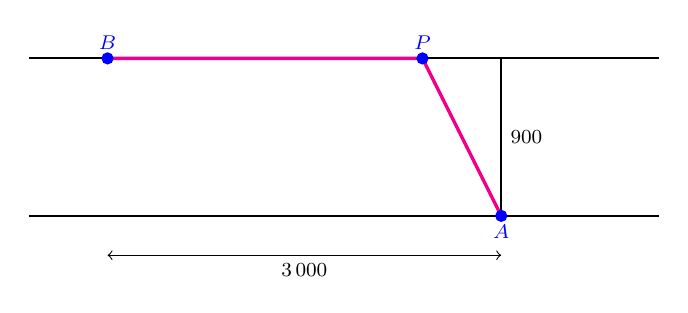
\begin{tikzpicture}
		% Draw horizontal line
		\draw[thick] (-4, 0) -- (4, 0) ;
		\draw[thick] (-4, -2) -- (4, -2) ;
		% Draw vertical line
		\draw[thick] (2, 0) -- (2, -2) node[midway, right] {900};
		\draw[<->] (2, -2.5) -- (-3, -2.5) node[midway, below] {$3 \,000$};
		% Draw the slanted line
		\draw[very thick, magenta] (-3, 0) -- (1, 0) -- (2, -2);
		% Add points
		\filldraw[blue] (-3, 0) circle (2pt) node[above] {$B$};
		\filldraw[blue] (1, 0) circle (2pt) node[above] {$P$};
		\filldraw[blue] (2, -2) circle (2pt) node[below] {$A$};
		
	\end{tikzpicture}
	\end{center}
	
	\shortans{$1\,800$}
	\loigiai{
	Đặt $BP=x  \Rightarrow PA = \sqrt{900^2+(3\,000-x)^2}$.\\
	Gọi $t_1$ là chi phí  kéo 1 mét cáp trên bờ và 	$t_2$ là chi phí để kéo $1$ mét cáp dưới nước. \\
	Theo bài cho $t_2=1{,}25t_1$ với $t_1,t_2>0$.\\
	Chi phí là $f(x)=xt_1+1{,}25t_1 \cdot\sqrt{900^2+(3\,000-x)^2} = t_1\left(x+1{,}25\sqrt{900^2+(3\,000-x)^2}\right)$. \\	
	Để chi phí là tiết kiệm nhất thì  $f(x)$ đạt giá trị nhỏ nhất  hay $\left(x+1{,}25\sqrt{900^2+(3\,000-x)^2}\right)$ đạt giá trị nhỏ nhất.\\
	Xét $g(x)=x+1{,}25\sqrt{900^2+(3\,000-x)^2}$ với $x \in (0;3\,000]$.\\
	Ta có $g'(x)=1-1{,}25\cdot\dfrac{3\,000-x}{\sqrt{900^2+(3\,000-x)^2}} \Rightarrow g'(x)=0 \Leftrightarrow x = 1\,800$.\\
	Bảng biến thiên
	\begin{center}
		
\begin{tikzpicture}
			\tkzTabInit[nocadre,lgt=1.5,espcl=2]{$x$ /1, $g'(x)$ /1,$g(x)$ /2}
			{$0$,$1 \, 800$,$3 \, 000$}%
			\tkzTabLine{ , - , 0 , + ,  }
			\tkzTabVar{ +/$g(0)$ / ,- / $g(1\,800)$ / , +/ $g(3000)$ / }
		\end{tikzpicture}
	\end{center}
	Ta tìm được $g(x)_{\min}=g(1\,800)=3\,675$ khi $x=1\,800$.\\
	Vậy để tiết kiệm chi phí nhất thì vị trí $P$ cách nhà máy $B$ là $1\,800 m$.
	}
\end{ex}

% #122 | Archive/SP_SauLuoi_2024-2025/SP_HKI/2-TN-DS-TLN-SGD-NamDinh-HK1-NH24-25.tex | mã gốc 2D1V3-6
\begin{ex}%[2D1V3-6]%[Đề thi khảo sát chất lượng HKI - SGD Nam Định]%[Vũ Hồng Ngọc]
	Một người quản lý ở một trang trại nuôi cá xác định rằng: Sau t tháng kể từ khi thả $300$ con cá $X$ (với $0 \leq t\leq 10$ ) thì khối lượng trung bình $m(t)$ tính theo kilogram của một con cá $X$ ước tính là $m(t)=0{,}45\Big(0{,}2+\dfrac{141}{155}t-0{,}05t^2\Big)$. Người này cũng nhận định tỉ lệ giữa số lượng cá $X$ còn sống trong ao so với số lượng cá $X$ thả ban đầu sau $t$ tháng kể từ ngày thả là $p(t)=\dfrac{31}{31+t}$. Biết rằng sản lượng cá $X$ tại một thời điểm được tính bằng tổng khối lượng của các con cá $X$ đã thả còn sống trong ao lúc đó. Hỏi với những nhận định trên của người quản lý thì dự kiến trong tối đa $10$ tháng nuôi, sản lượng cá $X$ lớn nhất có thể đạt được là bao nhiêu (kết quả tính theo đơn vị kilogram)?
\shortans{$459$}
\loigiai{
	Sản lượng cá $X$ là $S(t)=300\cdot m(t)\cdot p(t)$ với $0 \leq t\leq 10$.\\
	$\Rightarrow S(t)=300 \cdot0{,}45\cdot\Big(0{,}2+\dfrac{141}{155}t-0{,}05t^2\Big)\cdot \dfrac{31}{31+t}=\Big(0{,}2+\dfrac{141}{155}t-0{,}05t^2\Big)\cdot \dfrac{4\,185}{31+t}$.\\
	Ta tìm được $S_{\max}=459$ khi $t=8$.\\
	Vậy sản lượng cá $X$ lớn nhất có thể đạt được là $459$ kg.
}
\end{ex}

% #135 | Archive/SP_SauLuoi_2024-2025/SP_HKI/2-TN-DS-TLN-SGD-BacGiang-HKI-NH24-25.tex | mã gốc 2D1V3-6
\begin{ex}%[2D1V3-6]%[Dự Án Đợt 4 - De Thi HK1-2024-2025]%[Thầy Hải Toán]
Cho hai vị trí $A$, $B$ cách nhau $615$ m và cùng nằm về một phía bờ sông, giả sử bờ sông có dạng thẳng, khoảng cách từ $A$ và từ $B$ đến bờ sông lần lượt là $118$ m và $487$ m như hình vẽ sau:
	\begin{center}
	\begin{tikzpicture}[line join = round, line cap = round,>=stealth,font=\footnotesize,scale=1,declare function={ae=1.18;ab=6.15;bf=4.87;fe=sqrt(ab^2-ae^2);}]
	\path (0,0) coordinate (E)
	(0,ae) coordinate (A)
	(fe,0) coordinate (F)
	(fe,bf) coordinate (B)
	;
	\draw[thick] (E)--(A)node[left,pos=0.5]{$118$ m}--(B)node[above,pos=0.5,sloped]{$615$ m}--(F)node[above,pos=0.5,sloped]{$487$ m};
	\draw[shorten <= -1cm,shorten >= -1cm] (E)--(F)node[below,pos=0.5]{Sông};
	\draw[shorten <= -1cm,shorten >= -1cm] ($(E)+(0,-0.7)$)--($(F)+(0,-0.7)$);
	\foreach \x/\gm in {A/150,B/80,E/-130,F/-40} \draw[fill=black] (\x) circle (1pt) ($(\x)+(\gm:3.5mm)$)node[black]{$\x$};
	\end{tikzpicture}	
	\end{center}
	Một người đi từ $A$ đến bờ sông để lấy nước mang về $B$. Quãng đường ngắn nhất (tính theo đơn vị mét) mà người đó có thể đi gần với số nguyên dương nào nhất?
	\shortans[oly]{$96$}
\loigiai{
	\begin{center}
		\begin{tikzpicture}[line join = round, line cap = round,>=stealth,font=\footnotesize,scale=1,declare function={ae=1.18;ab=6.15;bf=4.87;fe=sqrt(ab^2-ae^2);}]
			\path (0,0) coordinate (E)
			(0,ae) coordinate (A)
			(fe,0) coordinate (F)
			(fe,bf) coordinate (B)
			($(A)!2!(E)$) coordinate (A')
			(intersection of A'--B and E--F) coordinate (C)
			($(B)!(A)!(F)$) coordinate (D)
			;
			\draw[thick] (E)--(A)node[left,pos=0.5]{$118$ m}--(B)node[above,pos=0.5,sloped]{$615$ m}--(D)node[above,pos=0.5,sloped]{$369$ m}--(F)node[right,pos=0.5]{$118$ m}
			(A)--(C)--(B) (E)--(A')node[left,pos=0.6]{$118$ m}--(C)
			(A)--(D)
			;
			\draw[shorten <= -1cm,shorten >= -1cm] (E)--(F);
			\foreach \x/\gm in {A/150,B/80,E/-130,F/-40,C/-90,A'/-90,D/0} \draw[fill=black] (\x) circle (1pt) ($(\x)+(\gm:3.5mm)$)node[black]{$\x$};
			\foreach \x/\y/\z in {C/E/A',B/F/C,A/D/B} \draw pic[draw,angle radius=2.5mm]{right angle=\x--\y--\z};
		\end{tikzpicture}	
	\end{center}
	Gọi $A'$ là điểm đối xứng của $A$ qua bờ sông $EF$. Suy ra $AC=A'C$.\\
	Quãng đường đi lấy nước là $S=AC+CB=A'C+CB\geqslant A'B$.\\
	Dấu \lq\lq$=$\rq\rq\ xảy ra khi và chỉ khi $A'$, $C$, $B$ thẳng hàng.\\
	Kẻ $AD\perp BF$ tại $D$ suy ra $AE=DF=118$ (m), $BD=BF-DF=487-118=369$ (m). $AD=EF=\sqrt{AB^2-BD^2}=\sqrt{615^2-369^2}=492$ (m).\\
	Gọi $EC=x$ ($0<x<492$), suy ra $FC=492-x$ (m).\\
	Ta có $\triangle CEA'\backsim \triangle CFB\Rightarrow \dfrac{CE}{CF}=\dfrac{EA'}{FB}\Rightarrow\dfrac{x}{492-x}=\dfrac{118}{487}\Rightarrow x\approx 95{,}96$ (m).\\
	Vậy giá trị nguyên dương gần nhất là $S=96$ (m).
}
\end{ex}

% #136 | Archive/SP_SauLuoi_2024-2025/SP_HKI/2-TN-DS-TLN-THPT-GiaDinh-TPHCM-HKI-NH24-25.tex | mã gốc 2D1V3-6
\begin{ex}%[2D1V3-6]%[Dự án A đợt 5, BCTuan]%[THPT Gia Định, TPHCM]
Công ty $X$ chuyên sản xuất một loại sản phẩm, bộ phận sản xuất ước tính rằng với $q$ sản phẩm được sản xuất trong một tháng thì tổng chi phí sẽ là $C(q)=8q^2+40q+1\,400$ (nghìn đồng) và mỗi sản phẩm công ty bán với giá $P(q)=1400-2q$ (nghìn đồng).
\choiceTF
{\True Chi phí mỗi tháng công ty phải bỏ ra để sản xuất $50$ sản phẩm là $23\,400$ (nghìn đồng)}
{Lợi nhuận bán được $q$ sản phẩm là $F(q)=-10q^2+1\,440q-1\,400$ (nghìn đồng)}
{Lợi nhuận cao nhất trong một tháng của công ty là hơn $50\,000$ (nghìn đồng)}
{\True Nếu số lượng sản phẩm bán ra trong một tháng nằm trong khoảng từ $60$ đến $70$ thì lợi nhuận sẽ được ước tính trong khoảng $44\,200$ đến $44\,840$ (nghìn đồng)}
\loigiai{
\begin{itemchoice}
	\itemch {\bf Đúng}.\\
Ta có chi phí mỗi tháng công ty bỏ ra để sản xuất $50$ sản phẩm là $C(50)=8\cdot 50^2+40\cdot 50+1\,400=23\,400$ (nghìn đồng).
	\itemch {\bf Sai}.\\
Lợi nhuận bán được $q$ sản phẩm là 
$$F(q)=q \cdot(1400-2q)-\left(8q^2+40q+1\,400\right)=-10q^2+1\,360q-1\,400\  \text {(nghìn đồng). }$$
	\itemch {\bf Sai}.\\
Ta có $F'(q)=-20q+1\,360$; $F'(q)=0 \Leftrightarrow q=68$.\\ 
Lập bảng biến thiên của $F(q)$ với $q>0$ ta có:
\begin{center}
	
\begin{tikzpicture}
		\tkzTabInit[lgt=1.2,espcl=3.5,deltacl=0.6]
		{$q$/1,$F'(q)$/1,$F(q)$/2.5}
		{$-\infty$,$0$,$+\infty$}
		\tkzTabLine{ ,+,0,-, }
		\tkzTabVar{-/$-1\,400$,+/$44\,840$,-/$-\infty$}
	\end{tikzpicture}
\end{center}
Vậy lợi nhuận cao nhất trong một tháng của công ty là hơn $44\,840$ (nghìn đồng).
	\itemch {\bf Đúng}.\\
Lập bảng biến thiên của $F(q)$ với $p\in[60;70]$ ta có
\begin{center}
	
\begin{tikzpicture}
		\tkzTabInit[lgt=1.2,espcl=3.5,deltacl=0.6]
		{$q$/1,$F'(q)$/1,$F(q)$/2.5}
		{$60$,$-68$,$70$}
		\tkzTabLine{ ,+,0,-, }
		\tkzTabVar{-/$44\,200$,+/$44\,840$,-/$44\,800$}
	\end{tikzpicture}
\end{center}
Từ bảng biến thiên ta có thấy nếu số lượng sản phẩm bán ra trong một tháng nằm trong khoảng từ $60$ đến $70$ thì lợi nhuận sẽ được ước tính trong khoảng $44\,200$ đến $44\,840$ (nghìn đồng).
\end{itemchoice}
}
\end{ex}

% #140 | Archive/SP_SauLuoi_2024-2025/SP_HKI/2-TN-DS-TLN-THPT-GiaDinh-TPHCM-HKI-NH24-25.tex | mã gốc 2D1V3-6
\begin{ex}%[2D1V3-6]%[Dự án A đợt 5,Nguyễn Tài Tuệ]%[THPT Gia Định, TPHCM]
	Trong một thí nghiệm y học, người ta cấy $1\,000 $ vi khuẩn vào môi trường dinh dưỡng. Bằng thực nghiệm, người ta xác định được số lượng vi khuẩn thay đổi theo thời gian bởi công thức:
	$N(t)=1\,000+\dfrac{100 t}{100+t^2}$ (con), trong đó $t$ là thời gian tính bằng giây. Tính số lượng vi khuẩn lớn nhất kể từ khi thực hiện cấy vi khuẩn vào môi trường dinh dưỡng.\par
	\shortans{$1\,005$}
	\loigiai{
		Xét hàm số $N(t)=1\,000+\dfrac{100 t}{100+t^2}(t>0)$.\\
		Ta có  $N'(t)=\dfrac{100 \cdot\left(100+t^2\right)-100 t \cdot 2 t}{\left(100+t^2\right)^2}=\dfrac{100 \cdot\left(100-t^2\right)}{\left(100+t^2\right)^2}$.\\
		Khi đó, với $t>0, N'(t)=0 \Leftrightarrow 100-t^2=0 \Leftrightarrow t^2=100 \Leftrightarrow t=10$.\\
		Bảng biến thiên của hàm số $N(t)$ như sau:
		\begin{center}
			
\begin{tikzpicture}
				\tkzTabInit[lgt=1.2,espcl=2]
				{$x$/0.7,$f’(x)$/.7,$f(x)$/2}
				{$0$,$10$,$+\infty$}
				\tkzTabLine{ ,+,z,-, }
				\tkzTabVar{-/$1\,000$,+/$1\,005$,-/$1\,000$}
			\end{tikzpicture}
		\end{center}		
		Căn cứ bảng biến thiên, ta thấy: Trên khoảng $(0 ;+\infty)$, hàm số $N(t)$ đạt giá trị lớn nhất bằng $1\,005$ tại $t=10$.\\
		Vậy số lượng vi khuẩn lớn nhất kể từ khi thực hiện cấy vi khuẩn vào môi trường dinh dưỡng là $1\,005$ con.}
\end{ex}

% #141 | Archive/SP_SauLuoi_2024-2025/SP_HKI/2-TN-DS-TLN-THPT-GiaDinh-TPHCM-HKI-NH24-25.tex | mã gốc 2D1V1-5
\begin{ex}%[2D1V1-5]%[Dự án A đợt 5,Nguyễn Tài Tuệ]%[THPT Gia Định, TPHCM]
	Quan sát một đàn ong trong $20$ tuần, người ta ước lượng được số lượng ong trong đàn bởi công thức $P(t)=\dfrac{20\,000}{1+10\,000 \mathrm{e}^{-t}}$, trong đó $t$ là thời gian tính theo tuần kể từ khi bắt đầu quan sát, $0 \leq t \leq 20$. Tại thời điểm nào thì số lượng ong của đàn tăng nhanh nhất (kết quả làm tròn đến hàng đơn vị của tuần).\par
	\shortans{$9$}
	\loigiai{
		Tốc độ thay đổi số lượng ong của đàn theo thời gian $t$ là		
		$$
		T(t)=P'(t)=2 \cdot 10^8 \cdot \dfrac{\mathrm{e}^{-t}}{\left(1+10\,000 \mathrm{e}^{-t}\right)^2}
		$$
		
		
		Ta có 
		\begin{eqnarray*}
			T'(t)&=&2 \cdot 10^8 \cdot \dfrac{-\mathrm{e}^{-t}\cdot\left(1+10\,000 \mathrm{e}^{-t}\right)^2-\mathrm{e}^{-t}\cdot 2 \cdot\left(1+10\,000 \mathrm{e}^{-t}\right) \cdot\left(-10\,000 \mathrm{e}^{-t}\right)}{\left(1+10\,000 \mathrm{e}^{-t}\right)^4}\\
			&=&2 \cdot 10^8 \cdot \dfrac{\mathrm{e}^{-t}\cdot\left(10\,000 \mathrm{e}^{-t}-1\right)}{\left(1+10\,000 \mathrm{e}^{-t}\right)^3}.
		\end{eqnarray*}
		
		$$T'(t)=0 \Leftrightarrow 10\,000-\mathrm{e}^t=0 \Leftrightarrow t=\ln 10\,000.$$
		
		Bảng xét dấu của đạo hàm
		\begin{center}
			
\begin{tikzpicture}
				\tkzTabInit[lgt=1.2,espcl=2]
				{$x$/0.7,$T’(x)$/.7 }
				{$0$,$\ln 10\,000$,$20$}
				\tkzTabLine{ ,+,z,-, }	 	 
			\end{tikzpicture}
		\end{center}	
		Từ đó, $T(t)$ đạt giá trị lớn nhất tại $t=\ln 10\,000 \approx 9$.\\
		Vậy đàn ong tăng nhanh nhất tại thời điểm khoảng $t=9$ tuần.}
\end{ex}

% #142 | Archive/SP_SauLuoi_2024-2025/SP_HKI/2-TN-DS-TLN-THPT-GiaDinh-TPHCM-HKI-NH24-25.tex | mã gốc 2D1V1-5
\begin{ex}%[2D1V1-5]%[Dự án A đợt 5,Nguyễn Tài Tuệ]%[THPT Gia Định, TPHCM]
	Vị trí của một vật chuyển động $s(t)$ (tính theo mét) vật đi được sau khoảng thời gian $t$ (tính theo giây), $t \geq 0$, được mô tả là một hàm số bậc ba có đồ thị như hình vẽ dưới đây.
	\begin{center}
		\begin{tikzpicture}[line join=round, line cap=round,>=stealth,thick,yscale=0.25,xscale=0.5]
			\tikzset{every node/.style={scale=0.9}}
			\draw[->] (-1.1,0)--(10.1,0) node[below] {$t(s)$};
			\draw[->] (0,-1.1)--(0,22.1) node[right] {$s(t)$ m};
			\draw (0,0) node [below left] {$O$};
			\draw[dashed] (3,0) node[below]{$3$}--(3,9)--(0,9) node[left]{$9$}  (7,0)node[below]{$7$} --(7,35/3)--(0,35/3) node[left]{$\tfrac{35}{3}$} (8,0) node[below]{$8$}--(8,52/3)--(0,53/3) node[left]{$\tfrac{52}{3}$};
			\begin{scope}
				\clip (-1,-1) rectangle (10,20);
				\draw[samples=200,domain=0:8.5,smooth,variable=\x] plot (\x,{1/6*((\x)^3)+-2*((\x)^2)+15/2*(\x)+0});
			\end{scope}
		\end{tikzpicture}
	\end{center}
	Trong $30$ giây đầu tiên, vật chuyển động nhanh dần bắt đầu từ thời điểm giây thứ mấy?\par
	\shortans{$3$}
	\loigiai{
		Gọi $s(t)=a t^3+b t^2+c t+d \quad(a \neq 0)$.\\
		Đồ thị hàm số $s(t)$ đi qua các điểm $O,(3 ; 9)$, $\left(7 ; \dfrac{35}{3}\right)$, $\left(8 ; \dfrac{52}{3}\right)$. 		
		$$
		\Rightarrow s(t)=\dfrac{1}{6}t^3-2 t^2+\dfrac{15}{2}t.
		$$
		Vật chuyển động nhanh dần nghĩa là vận tốc và gia tốc cùng dấu\\
		Xét vận tốc $v(t)=s'(t)=\dfrac{1}{2}t^2-4 t+\dfrac{15}{2}$ với $t \in[0 ; 30]$.\\
		$ v(t)=0 \Leftrightarrow \hoac{&t=3\\&t=5.}$\\
		Xét gia tốc $a(t)=v'(t)=t-4=0 \Leftrightarrow t=4$.\\
		Lập bảng xét dấu
		\begin{center}
			\begin{tabular}{|c|cccccccc|}
				\hline $t$ & $0$ & & $3$ & & $4$ & & $5$ & \\
				\hline Vận tốc $v(t)$ & & + & $0$ & - & $\mid$ & - & $0$ & + \\
				\hline Gia tốc $a(t)$ & & - & $\mid$ & - & $0$ & + & $\mid$ & + \\
				\hline$v(t) \cdot a(t)$ & & - & $0$ & + & $0$ & - & $0$ & + \\
				\hline
			\end{tabular}		 
		\end{center}
		Chuyển động nhanh dần từ giây thứ $3$.}
\end{ex}

% #143 | Archive/SP_SauLuoi_2024-2025/SP_HKI/2-TN-DS-TLN-THPT-GiaDinh-TPHCM-HKI-NH24-25.tex | mã gốc 2D1V2-7
\begin{ex}%[2D1V2-7]%[Dự án A đợt 5,Nguyễn Tài Tuệ]%[THPT Gia Định, TPHCM]
	\immini{	Một vật chuyển động với vận tốc $v$ (km/h) phụ thuộc vào thời gian $t$ (h) có đồ thị của hàm số dạng hàm bậc ba như hình bên dưới. Biết rằng tại thời điểm $t_1=1$ h vật có vận tốc $v_1=4$km/h  và tại thời điểm $t_2=2 $ h vật có vận tốc $v_2=1$ km/h. Tính vận tốc của vật tại thời điểm $t=4$ h.}{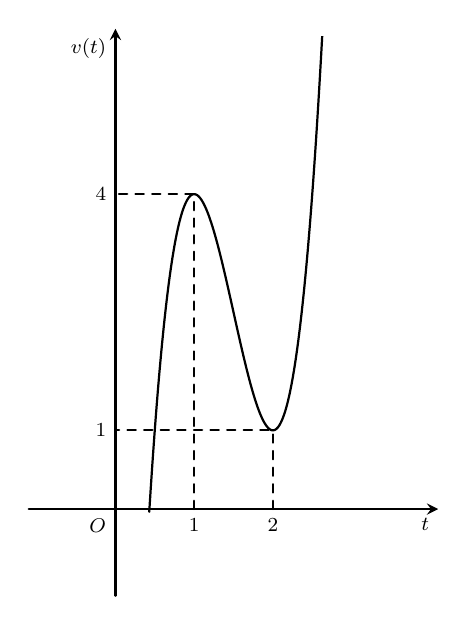
\begin{tikzpicture}[line join=round, line cap=round,>=stealth,thick]
			\tikzset{every node/.style={scale=0.9}}
			\draw[->] (-1.1,0)--(4.1,0) node[below left] {$t$};
			\draw[->] (0,-1.1)--(0,6.1) node[below left] {$v(t)$};
			\draw (0,0) node [below left] {$O$};
			\begin{scope}
				\clip (-1,-1) rectangle (4,6);
				\draw[samples=200,domain=0.43:3.5,smooth,variable=\x] plot (\x,{6*((\x)^3)+-27*((\x)^2)+36*(\x)+-11});
			\end{scope}
			\draw[dashed] (1,0) node[below] {$1$} --(1,4)--(0,4) node[left]{$4$} (2,0) node[below]{$2$}--(2,1) --(0,1) node[left]{$1$};
	\end{tikzpicture}}\par
	\shortans{$85$}
	\loigiai{
		Giả sử hàm số vận tốc có dạng $v(t)=a t^3+b t^2+c t+d, t>0$.\\
		Ta có: $v'(t)=3 a t^2+2 b t+c$.\\
		Dựa vào đồ thị hàm số, tại các thời điểm $t_1$, $t_2$ đồ thị hàm vận tốc đi qua các điểm cực trị $ (1 ; 4)$, $ (2 ; 1)$.\\
		Khi đó $\heva{&v(1)=4 \\&v'(1)=0 \\&v(2)=1 \\&v'(2)=0}\Leftrightarrow\heva{&a+b+c+d=4 \\&3 a+2 b+c=0 \\& 8 a+4 b+2 c+d=1 \\& 12 a+4 b+c=0}\Leftrightarrow\heva{&a=6 \\&b=-27 \\&c=36 \\& d=-11.}$\\
		Suy ra $v(t)=6 t^3-27 t^2+36 t-11 $ (km/h).\\
		Vậy vận tốc của vật tại thời điểm $t=4 $ h là  $v(4)=85$ km/h.}
\end{ex}

% #147 | Archive/SP_SauLuoi_2024-2025/SP_HKI/2-TN-DS-TLN-ChuyenLeQuyDon-NinhThuan-HKI-NH24-25.tex | mã gốc 2D1H5-8
\begin{ex}%[2D1H5-8]%[Dự án đề kiểm tra toán khối 12 HKI năm học 24-25 - Đợt 5 - Phạm Hoàng Đăng]%[Chuyên Lê Quý Đôn - Ninh Thuận]
	Lợi nhuận $N$ của một doanh nghiệp (triệu đồng) khi doanh nghiệp dùng số tiền $x$ để quảng cáo cho sản phẩm của doanh nghiệp đó ước tính theo công thức $N=f(x)=-0{,}1x^3+6x^2+400$, với $x \geq 0$.
	\choiceTF
	{Đạo hàm của hàm $f(x)$ là $f'(x)=-0{,}3x^2+12x+400$}
	{\True Khi tăng số tiền quảng cáo trong khoảng $(0; 40)$ thì lợi nhuận $N$ cũng tăng}
	{\True Phương án dùng số tiền quảng cáo $x$ sao cho lợi nhuận lớn nhất khi $x=40$}
	{\True Có hai phương án dùng số tiền đề quảng cáo sao cho lợi nhuận thu về là $800$}
	\loigiai{
		\begin{itemchoice}
			\itemch Hàm số có đạo hàm là $f'(x)=-0{,}3x^2+12x$.
			\itemch Ta có $f'(x)=0\Leftrightarrow \hoac{& x=0\\& x=40}$, ta có bảng biến thiên
			\begin{center}
				
\begin{tikzpicture}[>=stealth,line join=round,line cap=round,font=\footnotesize,scale=1]
					\tkzTabInit[nocadre,lgt=1.4,espcl=2.2,deltacl=0.5]
					{$x$/.7 ,$f'(x)$/.7,$f(x)$/2}
					{$0$, $40$ , $+\infty$}
					\tkzTabLine{$0$ , + , $0$ , - , }
					\tkzTabVar{-/$400$ , +/$3\,600$ , -/$-\infty$}
				\end{tikzpicture}
			\end{center}
			Từ bảng biến thiên ta thấy $f(x)$ đồng biến trên khoảng $(0;40)$ nên khi tăng số tiền quảng cáo trong khoảng từ $(0;40)$ thì lợi nhuận cũng tăng.
			\itemch Lợi nhuận đạt lớn nhất là $3\,600$ khi $x=40$.
			\itemch Đường thẳng $y=800$ cắt đồ thị hàm số $f(x)$ tại hai điểm trong khoảng $(0;+\infty)$ nên có hai phương án dùng số tiền để quảng cáo sao cho lợi nhuận thu về là $800$.
		\end{itemchoice}
	}
\end{ex}

% #153 | Archive/SP_SauLuoi_2024-2025/SP_HKI/2-TN-DS-TLN-ChuyenLeQuyDon-NinhThuan-HKI-NH24-25.tex | mã gốc 2D1V3-6
\begin{ex}%[2D1V3-6]%[CD-Lớp 12-HKI-Trường THPT chuyên Lê Quý Đôn-Ninh Thuận]%[VU Ngoc Hao]
	Một công ty sản xuất ra $x$ sản phẩm với giá bán một sản phẩm phụ thuộc vào số lượng sản phẩm được mô hình hóa theo phương trình $f(x)=26\,000-20x$. Tổng chi phí để sản xuất $x$ sản phẩm là $C(x)=x^3-1\,808x^2-2\,800x$. Hãy tìm số lượng sản phẩm cần sản xuất để công ty đạt lợi nhuận cao nhất?
	\shortans{$1238$}
	\loigiai{
		Hàm lợi nhuận $P(x)$ được tính bằng tổng doanh thu trừ đi tổng chi phí $P(x)=xf(x)-C(x)$.\\
		Thay các biểu thức đã cho vào, ta có:
		$$P(x)=x(26\,000-20x)-(x^3-1\,080x^2-2\,800x)=-x^3+1\,828x^2+28\,800x.$$
		Để tìm điểm cực đại, ta tính đạo hàm bậc nhất của hàm lợi nhuận $P(x)$ và cho bằng $0$:
		$P'(x)=-3x^2+3\,656x+28\,800$.\\
		$P'(x)=0\Leftrightarrow -3x^2+3\,656x+28\,800=0$.\\
		Giải phương trình bậc hai $-3x^2+3\,656x+28\,800=0$, ta tìm được hai nghiệm $x_1\approx -7{,}7$ và $x_2\approx 1\,237{,}7$.\\
		Vì số lượng sản phẩm phải là số dương, ta loại nghiệm $x_1$.\\
		Ta kiểm tra đạo hàm bậc hai để xác định xem $x_2$ là điểm cực đại hay cực tiểu\\
		$P''(x)=-6x+3\,656$; $P''(x_2)=P''(1237{,}7)\approx -4\,200<0$.\\
		Vì đạo hàm bậc hai âm, nên $x_2$ là điểm cực đại.\\
		Vậy số lượng sản phẩm cần sản xuất để công ty đạt lợi nhuận cao nhất xấp xỉ $1238$ sản phẩm.
	}
\end{ex}

% #160 | Archive/SP_SauLuoi_2024-2025/SP_HKI/2-TN-DS-TLN-THPT-NgoQuyen-HKI-HCM-NH23-24.tex | mã gốc 2D1H2-7
\begin{ex}%[2D1H2-7]%[Dự án đề KT Toán khối 12 HKI NH23-24-Trịnh Văn Cảnh]%[THPT Ngô Quyền - TPHCM]
	Một tàu đổ bộ tiếp cận Mặt Trăng theo cách tiếp cận thẳng đứng và đốt cháy các tên lửa hãm ở độ cao $250$ km so với bề mặt của Mặt Trăng. Trong khoảng $70$ giây đầu tiên kể từ khi đốt cháy các tên lửa hãm, độ cao $h$ của con tàu so với bề mặt của Mặt Trăng được tính gần đúng bởi hàm số $h(t)=-0{,}01 t^3+1{,}1t^2-30t+250$, trong đó $t$ là thời gian tính bằng giây và $h$ là độ cao tính bằng kilômét. Biết hàm số $h(t)$ đạt cực đại tại $t=\dfrac{a+b\sqrt{31}}{3}$ với $a$, $b$ là các số nguyên. Khi đó, giá trị của $a+b$ bằng bao nhiêu?
	\shortans{$120$}
	\loigiai{Xét hàm số $h(t)=-0{,}01 t^3+1{,}1t^2-30t+250$ với $0\le t\le 70$.\\
		Ta có $h'(t)=-0{,}03t^2+2{,}2t-30$.\\
		$h'(t)=0\Leftrightarrow t=\dfrac{\frac{220}{3} \pm \dfrac{20 \sqrt{31}}{3}}{2}=\dfrac{220 \pm 20 \sqrt{31}}{6}=\dfrac{110 \pm 10 \sqrt{31}}{3}\in [0;70]$.\\
		Bảng biến thiên
		\begin{center}
			
\begin{tikzpicture}
				\tkzTabInit[nocadre=false,lgt=1.2,espcl=2.5,deltacl=0.6]
				{$x$ /0.7,$y’$ /0.6,$y$ /2}%phần bắt buộc
				{$-\infty$,$\tfrac{110 - 10 \sqrt{31}}{3}$,$\tfrac{110 + 10 \sqrt{31}}{3}$,$+\infty$}
				\tkzTabLine{,-,0,+,0,-,}
				\tkzTabVar{+/$-\infty$,-/$4$,+/$0$,-/$+\infty$}
			\end{tikzpicture}
		\end{center}
		Từ bảng biến thiên, ta có hàm số $h(t)$ đạt cực đại tại $t=\dfrac{110+10\sqrt{31}}{3}$.\\
		Suy ra $a=100$, $b=10$. Khi đó $a+b=120$.
	}
\end{ex}

% #161 | Archive/SP_SauLuoi_2024-2025/SP_HKI/2-TN-DS-TLN-THPT-NgoQuyen-HKI-HCM-NH23-24.tex | mã gốc 2D1V3-6
\begin{ex}%[2D1V3-6]%[Dự án đề KT Toán khối 12 HKI NH23-24-Trịnh Văn Cảnh]%[THPT Ngô Quyền - TPHCM]
	Ông Nam cần xây dựng một bể chứa nước có dạng hình hộp chữ nhật không có nắp đậy để phục vụ cho việc tưới cây trong vườn. Do các điều kiện về diện tích vườn, ông Nam cần bể có thể tích là $36$ mét khối, đáy bể có chiều dài gấp hai lần chiều rộng và chiều rộng không quá $4$ mét, biết rằng chi phí vật liệu xây dựng mỗi mét vuông diện tích bề mặt là như nhau. Hỏi chiều cao bể nước bằng bao nhiêu mét để tổng chi phí vật liệu là nhỏ nhất?
	\shortans{$2$}
	\loigiai{Gọi chiều rộng của đáy bể là $x$ (mét) với $0<x\le 4$.\\
		Chiều dài của đáy bể là $2x$.\\
		Gọi $h$ (mét) là chiều cao của bể.\\
		Thể tích của bể là $V=h\cdot x \cdot 2x=2hx^2$.
		Suy ra $h=\dfrac{36}{2x^2}=\dfrac{18}{x^2}$. \qquad (1)\\
		Gọi $S$ là diện tích bề mặt của bể (không tính nắp).\\
		$S$ là tổng diện tích đáy và diện tích bốn mặt bên.\\
		Do đó $S=2x^2+2\cdot x\cdot h + 2\cdot 2x\cdot h=2x^2+6hx$. \qquad (2)\\
		Từ (1) và (2) suy ra $S=2x^2+6x\cdot \dfrac{18}{x^2}=2x^2+\dfrac{108}{x}$.\\
		Xét hàm số $f(x)=2x^2+\dfrac{108}{x}$ với $0<x\le 4$.\\
		Ta có $f'(x)=4x-\dfrac{108}{x^2}$.\\
		\begin{itemize}
			\item $f'(x)=0\Leftrightarrow 4x-\dfrac{108}{x^2}=0 \Leftrightarrow x=3<4$.
			\item $f'(x)>0\Leftrightarrow 4x-\dfrac{108}{x^2}>0 \Leftrightarrow x>3$.
			\item $f'(x)>0\Leftrightarrow 4x-\dfrac{108}{x^2}>0 \Leftrightarrow x<3$.
		\end{itemize}
		Bảng biến thiên
		\begin{center}
			
\begin{tikzpicture}
				\tkzTabInit[nocadre=false,lgt=1.2,espcl=2.5,deltacl=0.7]
				{$x$ /0.7,$f(x)’$ /0.6,$f(x)$ /2}%phần bắt buộc
				{$+\infty$,$3$,$+\infty$}
				\tkzTabLine{,-,0,+,}
				\tkzTabVar{+/$-\infty$,-/$f(3)$,+/$+\infty$}
			\end{tikzpicture}
		\end{center}
		Từ bảng biến thiên ta có 
		$\min\limits_{x\in (0;4]}f(x)=f(3)=54$ khi $x=3$.\\ Suy ra chiều cao của bể khi đó là $h=\dfrac{18}{3^2}=2$.\\
		Vậy để chi phí vật liệu là nhỏ nhất thì chiều cao của bể là $2$\, (m).
		
		
	}
\end{ex}

% #162 | Archive/SP_SauLuoi_2024-2025/SP_HKI/2-TN-DS-TLN-THPT-NgoQuyen-HKI-HCM-NH23-24.tex | mã gốc 2D1H4-4
\begin{ex}%[2D1H4-4]%[Dự án đề KT Toán khối 12 HKI NH23-24-Trịnh Văn Cảnh]%[THPT Ngô Quyền - TPHCM]
	Tổng chi phí để sản xuất $x$ sản phẩm của một xí nghiệp được tính theo công thức
	\[T(x)=2 x^2+x+25 \text { (nghìn đồng). }\]
	Chi phí trung bình của $1$ sản phẩm khi sản xuất được $x$ sản phẩm là $C(x)$. Xem $y=C(x)$ là một hàm số xác định trên khoảng $(0 ;+\infty)$, tiệm cận xiên của đồ thị hàm số này là đường thẳng $y=ax+b$. Giá trị của $a+b$ là bao nhiêu?
	\shortans{$3$}
	\loigiai{Chi phí trung bình của 1 sản phẩm khi sản xuất được $x$ sản phẩm là:
		\[C(x)=\dfrac{T(x)}{x}=\dfrac{2 x^2+x+25}{x}=2x+1+\dfrac{25}{x}.\]
		Ta thấy $\lim\limits_{x \to +\infty} [C(x) - (2x+1)]=\lim\limits_{x \to +\infty} \dfrac{25}{x}=0$.\\
		Do đó đường thẳng $y=2x+1$ là tiệm cận xiên của đồ thị hàm số $y=C(x)$.\\
		Suy ra $a=2$ và $b=1$.\\
		Vậy giá trị $a+b=2+1=3$.
	}
\end{ex}

% #172 | Archive/SP_SauLuoi_2024-2025/SP_GHKI/2-TN-DS-TLN-THPT-NguyenKhuyen-HCM-KTDK-NH23-24.tex | mã gốc 2D1V5-8
\begin{ex}%[2D1V5-8]%[Dự án A năm học 2024-2025 - THPT Nguyễn Khuyến - TPHCM]%[Khắc Thiên]
        Một con cá hồi bơi ngược dòng nước để vượt một khoảng cách là $300$ km. Vận tốc dòng nước là $6$ (km/h). Nếu vận tốc bơi của cá khi nước đứng yên là $v$ (km/h) thì năng lượng tiêu hao của cá trong $t$ giờ được cho bởi công thức $E(v)=cv^{3}t$ (trong đó $c$ là hằng số dương, $E$ được tính bằng đơn vị Jun). Cá bơi ngược dòng quãng đường $300$ km trên trong khoảng thời gian $t$ với vận tốc bằng bao nhiêu để năng lượng tiêu hao là thấp nhất?
        \shortans{$3$}
        \loigiai{Vận tốc của cá khi bơi ngược dòng nước là $v-6$ (km/h).\\
            Thời gian để cá vượt qua quãng đường $300$ km là $t=\dfrac{300}{v-6}$ (giờ).\\
            Năng lượng tiêu hao của cá để vượt qua quãng đường đó là $E(v)=cv^3 \cdot \dfrac{300}{v-6}$ (J) với $v>6$.\\
            Ta có
            \begin{eqnarray*}
                &&E'(v)=600 c \cdot \frac{v^2(v-9)}{(v-6)^2} \\
                \Rightarrow&& E'(v)=0 
                \Leftrightarrow \hoac{&v=9\in \left(6;+\infty \right) \\&v=6\notin\left(6;+\infty\right) } \\
                \Rightarrow&& E(9)=72900c.
            \end{eqnarray*}
            Bảng biến thiên
            \begin{center}
                \begin{tikzpicture}[>=stealth, scale=1]
                \tkzTabInit[lgt=2,espcl=2.7]
                {$v$/0.8,$E^{\prime}(v)$/0.8,$E(v)$/3}
                {$-\infty$,$6$,$9$,$+\infty$}
                \tkzTabLine{,h,d,-,0,+,}
                \path
                (N22)node[shift={(0.5,-0.2)}](A){$ $}
                (N33)node[shift={(0,0.2)}](B){$72900c$}
                (N42)node[shift={(0,-0.2)}](C){$ $};
                \foreach\X/\Y in{A/B,B/C}\draw[->](\X)--(\Y);
                \filldraw[pattern=north west lines, draw=none] (T11) rectangle (N23);
                %\draw[,double distance=2pt](N22)--(N23);
            \end{tikzpicture}
            \end{center}
            Dựa vào bảng biến thiên, ta có
            \begin{eqnarray*}
                E_{\min}=72900c \text { khi } v=9(km/h). 
            \end{eqnarray*}
            Vậy để ít tiêu hao năng lượng nhất, cá phải bơi với vận tốc là $v=9$ (km/h).\\
            Vận tốc khi bơi ngược dòng nước là $v-6=9-6=3$ (km/h).
        }
    \end{ex}

% #181 | Archive/SP_SauLuoi_2024-2025/SP_GHKI/2-TN-DS-TLN-THPT-BuiThiXuan-GHKI-NH24-25.tex | mã gốc 2D1H1-5
\begin{ex}%[2D1H1-5]%[CTST - Lớp 12 - Ôn tập học kì 1 - THPT Bùi Thị Xuân]%[Thanh Phát]
	Một vật đang đứng yên thì bắt đầu chuyển động theo quy luật $s(t)=-t^3+3t^2+6t$, với $t$ (giây) là khoảng thời gian tính từ lúc vật bắt đầu chuyển động và $s$ (mét) là quãng đường vật đi được trong khoảng thời gian đó. Hỏi vật tăng tốc trong khoảng thời gian bao nhiêu giây tính từ lúc bắt đầu chuyển động?
	\shortans{1}
	\loigiai{Vận tốc của vật là $v(t)=s'(t)=-3t^2+6t+6$.\\
		Ta có $v'(t)=-6t+6$.\\
		Cho $v'(t)=0 \Leftrightarrow t=1$.\\
		Bảng biến thiên\\
		\begin{center}
			
\begin{tikzpicture}
				\tkzTabInit[lgt=1.2,espcl=2.5,deltacl=0.6]
				{$t$/0.6,$v'(t)$/0.6,$v(t)$/2}{$0$,$1$,$+\infty$}
				\tkzTabLine{,+,0,-,}
				\tkzTabVar{-/$6$,+/$9$,-/$-\infty$}
			\end{tikzpicture}
		\end{center}
		Dựa vào bảng biến thiên, ta thấy $v(t)$ tăng khi $t\in (0;1)$. Vậy vật tăng tốc trong khoảng thời gian từ gian $1$ giây tính từ lúc bắt đầu chuyển động.
	}
\end{ex}

% #182 | Archive/SP_SauLuoi_2024-2025/SP_GHKI/2-TN-DS-TLN-THPT-BuiThiXuan-GHKI-NH24-25.tex | mã gốc 2D1V4-3
\begin{ex}%[2D1V4-3]%[Lớp 12 - Ôn tập giữa học kì 1 năm 24-25 - Bùi Thị Xuân TP HCM]%[Phạm Văn Long]
	Một công ty sản xuất máy tính đã xác định được rằng: tính trung bình một nhân viên có thể lắp ráp được $P(x)=\dfrac{500x}{4x+25}$ bộ phận mỗi ngày sau $x$ ngày được đào tạo, với $x \geq 0$. Xem $y=P(x)$ là một hàm số xác định trên $[0;+\infty)$ thì $y=a$ là đường tiệm cận ngang của đồ thị hàm số. Xác định giá trị $a$.
	\shortans{125}
	\loigiai{
	Ta có $\lim\limits_{x \to +\infty}\dfrac{500x}{4x+25}=125$ nên $y=125$ là đường tiệm cận ngang của đồ thị hàm số.\\ Vậy $a=125$.
	}
\end{ex}

% #189 | Archive/SP_SauLuoi_2024-2025/SP_GHKI/1-TN-DS-TLN-THPT-NguyenThuongHien-TPHCM-GHKI-NH24-25.tex | mã gốc 2D1C3-6
\begin{ex}%[GHK1-THPT Nguyễn Thượng Hiền-TPHCM]%[Nguyễn Cường]%[2D1C3-6]
Trên $4$ cạnh của khu vườn hình chữ nhật $ABCD$ có kích thước $30$ (m)$\times 72$ (m), người ta đặt $4$ trạm quan sát tại $4$ điểm $M$, $N$, $P$, $Q$ và xây dựng đường đi giữa các trạm như hình vẽ.
\begin{center}
\begin{tikzpicture}[scale=1, font=\footnotesize, line join=round, line cap=round, >=stealth]
\path
(0,0) coordinate (A)++(0:7.2)coordinate(B)++(90:3)coordinate(C)++(180:7.2)coordinate(D)
(A)++(0:2.4)coordinate(N)
(A)++(90:1)coordinate(M)
(C)++(-90:2)coordinate(P)
(C)++(180:4.8)coordinate(Q)
($(A)!.5!(M)$)node[left]{$10$ m}
($(A)!.5!(N)$)node[below]{$24$ m}
;
\draw (A)--(B)--(C)--(D)--cycle
(M)--(N)
;
\draw (Q)--(M) (N)--(P)--(Q);
\draw[<->]($(A)+(-1,0)$)--($(D)+(-1,0)$)node[midway,left]{$30$ m}
;
\draw[<->]($(A)+(0,-1)$)--($(B)+(0,-1)$)node[midway,below]{$72$ m}
;
\foreach \x/\g in {A/-90,B/-90,C/90,D/90,N/-90,P/0,Q/90,M/180} \fill (\x) circle(1pt)++(\g:0.3) node{$\x$};
\end{tikzpicture}
\end{center}
Biết $AM=10$ m, $AN=24$ m, điểm $P$ thuộc cạnh $BC$, điểm $Q$ thuộc cạnh $CD$ và $PQ\parallel MN$. Tìm giá trị nhỏ nhất của tổng độ dài $MN+NP+PQ+QM$.
\shortans{130}
\loigiai{
	\begin{center}
		\begin{tikzpicture}[scale=1, font=\footnotesize, line join=round, line cap=round, >=stealth]
			\path
			(0,0) coordinate (A)++(0:7.2)coordinate(B)++(90:3)coordinate(C)++(180:7.2)coordinate(D)
			(A)++(0:2.4)coordinate(N)
			(A)++(90:1)coordinate(M)
			(C)++(-90:2)coordinate(P)
			(C)++(180:4.8)coordinate(Q)
			($(A)!.5!(M)$)node[left]{$10$ m}
			($(A)!.5!(N)$)node[below]{$24$ m}
			($(M)!2!(D)$)coordinate(M')
			($(N)!2!(B)$)coordinate(N')
			;
			\draw (A)--(B)--(C)--(D)--cycle
			(M)--(N)
			(D)--(M')--(Q) (P)--(N')--(B)
			;
			\draw (Q)--(M) (N)--(P)--(Q) ;
			\draw[<->]($(A)+(-1,0)$)--($(D)+(-1,0)$)node[midway,left]{$30$ m}
			;
			\draw[<->]($(A)+(0,-1)$)--($(B)+(0,-1)$)node[midway,below]{$72$ m}
			;
			\foreach \x/\g in {A/-90,B/-90,C/90,D/180,N/-90,P/30,Q/90,M/180,M'/90,N'/0} \fill (\x) circle(1pt)++(\g:0.3) node{$\x$};
		\end{tikzpicture}
	\end{center}
Gọi $M'$ là điểm đối xứng của $M$ qua $D$ nên $MD=M'D=20$ (m).\\
Gọi $N''$ là điểm đối xứng của $N$ qua $B$ nên $NB=N'B=48$ (m).\\
Suy ra $AM'=50$ (m) và $AN'=120$ (m).\\
$\triangle AM'N'$ vuông tại $A$ có $M'N'=\sqrt{AM'^2+AN'^2}=\sqrt{50^2+120^2}=130$ (m).
\allowdisplaybreaks
\begin{eqnarray*}
	S&=&MN+NP+PQ+QM\\
	&=&MN+N'P+PQ+QM'\\
	&\ge& M'N'=130.
\end{eqnarray*}
Vậy tổng độ dài ngắn nhất là $130$ (m) khi $M'$, $Q$, $P$, $N'$ thẳng hàng nhau.
}
\end{ex}

% #195 | Archive/SP_SauLuoi_2024-2025/SP_GHKI/2-TN-DS-TLN-THPT-TayThanh-TpHCM-GHKI-NH24-25.tex | mã gốc 2D1V4-4
\begin{ex}%[2D1V4-4]%[2-TN-DS-TLN-THPT-TayThanh-TpHCM-GHKI-NH24-25]%[Phúc Chương]
	Một ống khói của nhà máy điện hạt nhân có mặt cắt là một hypebol $(H)$ có phương trình chính tắc là $\dfrac{x^2}{27^2}-\dfrac{y^2}{40^2}=1$ (xem hình dưới). Hai nhánh bên trên của $Ox$ của $(H)$ là đồ thị $(C)$ của hàm số $y=\dfrac{40}{27}\sqrt{x^2-27^2}$ (phần nét liền đậm). Đường thẳng $y=\dfrac{a}{b}x$ là một tiệm cận xiên của $(C)$. Biết rằng $a\in\mathbb{N}$, $b\in\mathbb{N}^*$, $\dfrac{a}{b}$ là phân số tối giản. Tính $a+b$.
	\begin{center}
		\begin{tikzpicture}[scale=.5, font=\footnotesize, line join=round, line cap=round, >=stealth,xscale=1/10,yscale=1/10]
			\draw[->] (-90,0)--(90,0)node[below]{$x$};
			\draw[->] (0,-40)--(0,80)node[left]{$y$};
			\begin{scope}
				\clip (0,-40) rectangle (90,80);
				\draw[smooth,samples=100,domain=27:90] 
				plot(\x,{(40/27)*(sqrt((\x)^2-27^2))});
				\draw[dashed, smooth,samples=100,domain=27:90] 
				plot(\x,{-(40/27)*(sqrt((\x)^2-27^2))});
			\end{scope}
			\begin{scope}
				\clip (0,-40) rectangle (-90,80);
				\draw[smooth,samples=100,domain=-90:-27] 
				plot(\x,{(40/27)*(sqrt((\x)^2-27^2))});
				\draw[dashed, smooth,samples=100,domain=-90:-27] 
				plot(\x,{-(40/27)*(sqrt((\x)^2-27^2))});
			\end{scope}
			\fill (0,0)node[below left]{$O$} circle (15pt);
			\foreach \x in {-80,-60,-40,-20,20,40,60,80}{\fill (\x,0)node[below]{$\x$} circle (15pt);}
			\foreach \x in {-20,20,40,60}{\fill (0,\x)node[left]{$\x$}circle(15pt);}
		\end{tikzpicture}
	\end{center}
	\shortans{67}
	\loigiai{Đặt $f(x)=\dfrac{40}{27}\sqrt{x^2-27^2}$.\\
	Ta có $\lim\limits_{x \to +\infty} \dfrac{f(x)}{x} = \lim\limits_{x \to +\infty} \dfrac{40}{27} \dfrac{\sqrt{x^2-27^2}}{x} = \lim\limits_{x \to +\infty} \dfrac{40}{27} \cdot \dfrac{\sqrt{1-\dfrac{27^2}{x^2}}}{1} = \dfrac{40}{27}$.\\
	Lại có $\lim\limits_{x \to +\infty} \left(f(x)-\dfrac{40}{27}x\right) = \lim\limits_{x \to +\infty} \left(\dfrac{40}{27} \sqrt{x^2-27^2} - \dfrac{40}{27}x \right) = \dfrac{40}{27} \lim\limits_{x \to +\infty} \dfrac{-27^2}{\sqrt{x^2-27^2}+x}=0$.\\
	Do đó đồ thị hàm số có một tiệm cận xiên là $y=\dfrac{40}{27}x$. Suy ra $a=40$ và $b=27$.\\
	Vậy $a+b=67$.}
\end{ex}

% #196 | Archive/SP_SauLuoi_2024-2025/SP_GHKI/2-TN-DS-TLN-THPT-TayThanh-TpHCM-GHKI-NH24-25.tex | mã gốc 2D1V3-6
\begin{ex}%[2D1V3-6]%[2-TN-DS-TLN-THPT-TayThanh-TpHCM-GHKI-NH24-25]%[Phúc Chương]
	\immini[thm]{
	Một công ty muốn làm một đường ống dẫn từ vị trí $A$ trên bờ biển (xem bờ biển là đường thẳng $AH$) đến vị trí $B$ trên hòn đảo. Khoảng cách từ điểm $B$ đến bờ biển là $BH=6$ km (xem hình bên). Giá tiền để xây dựng đường ống trên bờ là $80\,000$ USD mỗi kilômét và giá tiền xây dựng đường ống trên biển là $170\,000$ USD mỗi kilômét, biết rằng $AH=10$ km. Cần xác định vị trí điểm $C$ trên đoạn $AH$ để khi lắp ống dẫn theo đường gấp khúc $ACB$ thì chi phí công ty bỏ ra là thấp nhất. Hỏi độ dài đoạn đường $HC$ là bao nhiêu km? (ghi kết quả dưới dạng số thập phân).}
	{\begin{tikzpicture}[scale=.7, font=\footnotesize, line join=round, line cap=round, >=stealth]
			\path (0,0) coordinate (H)
			(0,6) coordinate (B)
			(10,0) coordinate (A)
			(6,0) coordinate (C)
			($(B)!0.5!(H)$) coordinate (M1)node[above, rotate = 90]{$BH=6$ km}
			($(H)!0.5!(C)$) coordinate (M2)node[above]{$x=?$}
			($(H)!0.5!(A)$) coordinate (M3)node[below]{$AH=10$ km};
			\draw (A)--(H)--(B)--(C);
			\foreach \x/\y in {B/90,H/180,C/60,A/0}{\fill (\x)node[shift={(\y:4mm)}]{$\x$} circle (1.2pt);}
	\end{tikzpicture}}
	\shortans{3,2}
	\loigiai{Gọi $x$ km là độ dài $HC$ ($0\le x \le 10$). Khi đó, $CA=10-x$ (km) và $BC=\sqrt{36+x^2}$ (km).\\
	Chi phí xây dựng đường ống là
	\[C(x) = BC \cdot 170 + CA \cdot 80 = 170\sqrt{36+x^2} + 80 \cdot (10-x)\quad (\text{nghìn USD}).\]
	Ta tìm $x \in [0;10]$ sao cho $C(x)$ nhỏ nhất.\\
	Ta có $C'(x)=170\cdot\dfrac{x}{\sqrt{36+x^2}}-80 = \dfrac{170x -80\sqrt{36+x^2}}{\sqrt{36+x^2}}, \forall x \in [0;10]$.\\
	$C'(x)=0 \Leftrightarrow 17x - 8\sqrt{36+x^2}=0 \Leftrightarrow 225x^2=2\,304 \Leftrightarrow x =\dfrac{16}{5}$.\\
	Ta có $C(0)=1\,820$, $C(10)\approx 1\,982{,}5$ và $C\left(\dfrac{16}{5}\right)=1\,700$.\\
	Vậy tại $x=\dfrac{16}{5}$ thì $C(x)$ đạt giá trị nhỏ nhất. Hay $HC=\dfrac{16}{5}=3{,}2$ thì chi phí làm đường ống là nhỏ nhất.}
\end{ex}

% #201 | Archive/SP_SauLuoi_2024-2025/SP_GHKI/2-TL-TN-TLN-THPT-PhamVanSang-HCM-GHKI-NH24-25€.tex | mã gốc 2D1H5-8
\begin{ex}%[2D1H5-8]%[Dự án đề kiểm tra Toán khối 12 GHKI NH24-25 - Dot 1 - Thành Đức Trung]%[THPT Phạm Văn Sang - TP Hồ Chí Minh]
	\immini
	{
		Cho một tấm nhôm hình vuông cạnh $12$cm. Người ta cắt ở bốn góc của tấm nhôm bốn hình vuông bằng nhau, mỗi hình vuông có cạnh bằng $x$(cm), rồi gập tấm nhôm lại để được một cái hộp có dạng hình hộp chữ nhật không có nắp (Tham khảo hình vẽ). Giá trị của $x$ bằng bao nhiêu centimet (cm) để thể tích của khối hộp đó là lớn nhất?
	}
	{
		\begin{tikzpicture}[blue,thick,font=\footnotesize, line cap=round, line join=round, >=stealth]
			\def\a{.5} \def\goc{30}
			\path 	
			(0:0) coordinate (A)
			(0:6*\a) coordinate (B)
			(90:6*\a) coordinate (D)
			($(B)+(D)-(A)$) coordinate (C)
			($(A)!1/6!(B)$) coordinate (AB) ($(B)!1/6!(A)$) coordinate (BA)
			($(D)!1/6!(C)$) coordinate (DC) ($(C)!1/6!(D)$) coordinate (CD)
			($(A)!1/6!(D)$) coordinate (AD) ($(D)!1/6!(A)$) coordinate (DA)
			($(B)!1/6!(C)$) coordinate (BC) ($(C)!1/6!(B)$) coordinate (CB)
			(intersection of AB--DC and AD--BC) coordinate (a)
			(intersection of BA--CD and BC--AD) coordinate (b)
			(intersection of CB--DA and CD--BA) coordinate (c)
			(intersection of DC--AB and DA--CB) coordinate (d)
			($(BC)+(0:5mm)$) coordinate(m)
			($(m)+(90:2*\a)$) coordinate(n)
			($(n)+(0:4*\a)$) coordinate(p)
			($(m)+(0:4*\a)$) coordinate(q)
			($(m)+(\goc:3*\a)$) coordinate(x)
			($(n)+(\goc:3*\a)$) coordinate(y)
			($(p)+(\goc:3*\a)$) coordinate(u)
			($(q)+(\goc:3*\a)$) coordinate(v)
			(intersection of n--p and x--y) coordinate(i)
			;
			\draw (A)--(B)--(C)--(D)--cycle (AB)--(a)--(AD) (BC)--(b)--(BA) (CD)--(c)--(CB) (DA)--(d)--(DC)	;
			\draw[blue] (m)--(n)--(p)--(q)--cycle (n)--(p)--(u)--(y)--cycle (u)--(v)--(q) (y)--(i);
			\draw[blue,dashed] (m)--(x)--(v) (x)--(i);
			\draw[blue] (a)--(b)--(c)--(d)--cycle;
			\fill[blue] (A)--(AB)--(a)--(AD) (B)--(BC)--(b)--(BA) (C)--(CD)--(c)--(CB) (D)--(DA)--(d)--(DC);
			\draw[<->] ($(A)+(180:3.25mm)$)--($(D)+(180:3.25mm)$) node[pos=.5,fill=white,xshift=-6mm]{$12\,\mathrm{cm}$};
			\path 
			(B)node[right,yshift=-4pt]{}
			(B)--(BC)node[right,pos=1/2,xshift=-2pt]{}
			(C)--(CB)node[right,pos=1/2,xshift=-2pt]{$x\,\mathrm{cm}$}
			;
		\end{tikzpicture}
	}
	\shortans{$2$}
	\loigiai
	{
		Sau khi cắt $4$ góc và gập lại ta được hình hộp chữ nhật có kích thước đáy $12-2x$ (cm) và chiều cao là $x$.\\
		Khi đó thể tích khối hộp thu được là $V=(12-2x)^2x=144x-48x^2+4x^3$.\\
		Xét $V=f(x)=144x-48x^2+4x^3$ có $f'(x)=144-96x+12x^2=0 \Leftrightarrow \hoac{ & x=2 \\ &x=6.}$\\
		Ta có bảng biến thiên của $f(x)$
		
		\begin{center}
			
\begin{tikzpicture}[scale=1]
				\tkzTabInit[nocadre=false, lgt=1.2, espcl=2.5, deltacl=0.6]{$x$/0.6, $y'$/0.6, $y$/2}{$0$, $2$, $6$}
				\tkzTabLine{,+,0,-,}
				\tkzTabVar{-/$0$, +/$128$, -/$0$}
			\end{tikzpicture}
		\end{center}
		Từ bảng biến thiên suy ra $x=2$ thì $f(x)$ đạt giá trị lớn nhất.\\
		Vậy $x=2$ cm thì thể tích khối hộp lớn nhất.
	}
\end{ex}

% #205 | Archive/SP_SauLuoi_2024-2025/SP_GHKI/2-TL-TN-TLN-THPT-PhamVanSang-HCM-GHKI-NH24-25€.tex | mã gốc 2D1H1-5
\begin{ex}%[2D1H1-5]%[CTST - Lớp 12 - Đề chính thức - THPT Phạm Văn Sáng - TPHCM]%[Hiếu Mai]
	Kính viễn vọng không gian Hubble được đưa vào vũ trụ ngày 24/4/1990 bằng tàu con thoi Discovery.
	Vận tốc của tàu con thoi trong sứ mệnh này, từ lúc cất cánh tại thời điểm $t=0~(\text{s})$ cho đến khi tên lửa đẩy được phóng đi tại thời điểm $t=126~(\text{s})$, được cho bởi hàm số sau
	$v(t) = 0{,}001302t^3 - 0{,}09029t^2+23$,
	($v(t)$ được tính bằng $\text{feet}/\text{s}$, $1~\text{feet} = 0{,}3048~\text{m}$).
	(\textit{Nguồn: J. Stewart, Calculus Seventh Edition, Brooks/Cole, CENGAGE Learning 2012}).
	Gia tốc của tàu con thoi được tính bằng công thức $a(t)=v'(t)$ sẽ tăng trong khoảng thời gian $(a,b)$ đơn vị (s) tính từ thời điểm cất cánh cho đến khi tên lửa đẩy được phóng đi.
	Tính $a+b$ (quy tròn đến hàng đơn vị).
	\shortans{$149$}
	\loigiai{
		Trong khoảng thời gian $t=0$ đến $t=126~\text{s}$, vận tốc của tên lửa là
		$$
		v(t) = 0{,}001302t^3 - 0{,}09029t^2+23.
		$$
		Do đó gia tốc của nó là
		$$
		a(t)
		= v'(t)
		= 0{,}003906 t^2 - 0{,}18058 t.
		$$
		Xét đạo hàm của gia tốc
		$$
		a'(t)
		= 0{,}007812 t - 0{,}18058.
		$$
		Cho $a'(t)=0$, ta được
		$$
		0{,}007812 t - 0{,}18058
		\Rightarrow
		t \approx 23~\text{s}.
		$$
		Lập bảng biến thiên của $a(t)$:
		\begin{center}
			
\begin{tikzpicture}
				\tkzTabInit[lgt=2,espcl=3]
				{$t$/1, $a'(t)$/1, $t$/2}
				{$0$, $23$, $126$}
				\tkzTabLine{, -, z, +}
				\tkzTabVar{+/$a(0)$, -/$a(23)$, +/$a(126)$}
			\end{tikzpicture}
		\end{center}
		Dựa vào bảng biến thiên trên, ta thấy $a(t)$ tăng trong khoảng $(23;126)$. 
		\\
		Do đó $a=23$ và $b=126$.
		\\
		Vậy $a+b=149$.
	}
\end{ex}

% #211 | Archive/SP_SauLuoi_2024-2025/SP_GHKI/2-TN-DS-TLN-TH-THCS-THPTLeThanhTong-TPHCM-NH24-25.tex | mã gốc 2D1V3-6
\begin{ex}%[2D1V3-6]%[Dự án đề KTDK Lớp 12 - NH24-25 - THPT Lê Thánh Tông - TPHCM]%[Nguyễn Ngọc Huy Trường]
	Một công ty chi một trăm triệu đồng để sản xuất các thùng sơn hình trụ có dung tích $5$ lít. Biết rằng chi phí để làm mặt xung quanh thùng đó là $100\,000$ đ/m$^2$, chi phí để làm mỗi mặt đáy của thùng đó là $120\,000$ đ/m$^2$. Hãy tính số thùng sơn tối đa mà công ty đó sản xuất được (giả sử chi phí các mối nối không đáng kể).
	\shortans{5\,813}
	\loigiai{
		Gọi $r$, $h$ (m) lần lượt là bán kính đáy và chiều cao của thùng sơn hình trụ ($r,h>0$). \\
		Do thùng sơn có thể tích $5$ lít nên $\pi r^2 h = 5\cdot 10^{-3}\Leftrightarrow h = \dfrac{5\cdot 10^{-3}}{\pi r^2}$. \\
		Diện tích xung quanh thùng là $S_\text{xq} = 2\pi rh = 2\pi r \cdot \dfrac{5\cdot 10^{-3}}{\pi r^2} = \dfrac{10^{-2}}{r}$. \\
		Diện tích đáy thùng là $S_\text{đáy} = \pi r^2$. \\
		Chi phí sản xuất thùng sơn là
		\allowdisplaybreaks
		\begin{eqnarray*}
			& & 100\cdot S_\text{xq} + 120\cdot 2\cdot S_\text{đáy} \\
			& =& 100\cdot \dfrac{10^{-2}}{r} + 120\cdot 2\cdot \pi r^2  \\
			& = & \dfrac{1}{r} + 240\pi r^2 \\
			& = & C(r) \ \text{(nghìn đồng)}.
		\end{eqnarray*}
		Ta có $C'(r) = \dfrac{-1}{r^2} + 480\pi r$. Khi đó $C'(r) = 0\Leftrightarrow 480\pi r = \dfrac{1}{r^2}\Leftrightarrow r = \sqrt[3]{\dfrac{1}{480\pi}} = r_0$. \\
		Bảng biến thiên
		\begin{center}
			
\begin{tikzpicture}[scale=1, font=\footnotesize, line join=round, line cap=round, >=stealth]
			\tkzTabInit[nocadre=false,lgt=1.2,espcl=2.5,deltacl=0.6]
			{$x$/0.7, $y'$/0.7, $y$/2.5}
			{$0$,$r_0$,$+\infty$}
			\tkzTabLine{,-,0,+,}
			\tkzTabVar{+/$+\infty$,-/$C(r_0)$,+/$+\infty$}
			\end{tikzpicture}
		\end{center}
		Từ bảng biến thiên, ta suy ra chi phí sản xuất thùng sơn thấp nhất là $C(r_0) \approx 17{,}2$ (nghìn đồng). \\
		Do đó số thùng sơn mà công ty sản xuất được là $\dfrac{100\cdot 10^6}{17{,}2\cdot 10^3} \approx 5\,813{,}6$. \\
		Vậy  số thùng sơn tối đa mà công ty sản xuất được là $5\,813$.
	}
\end{ex}

% #214 | Archive/SP_SauLuoi_2024-2025/SP_GHKI/2-TN-DS-TLN-TH-THCS-THPTLeThanhTong-TPHCM-NH24-25.tex | mã gốc 2D1V5-8
\begin{ex}%[2D1V5-8]%[2-TN-DS-TLN-THPT-le-thanh-tong-tp-hcm-KTDT-13-10-2024]%[Phúc Chương]
	\immini[thm]{Một hàng rào cao $2{,}4$ mét được đặt song song và cách bước tường của ngôi nhà một khoảng bằng  $1{,}5$ mét. Chiều dài ngắn nhất của cây thang để nó đứng dưới đất vươn qua hàng rào tựa vào ngôi nhà (xem hình vẽ) là bao nhiêu mét (làm tròn kết quả đến hàng phần chục)?}
	{\begin{tikzpicture}[scale=0.7, font=\footnotesize, line join=round, line cap=round, >=stealth, transform shape]
		\draw[fill=blue!30!white] (0,0)--(5,1)--(5,4)--(0,3)--cycle;
		\draw[fill=blue!30!black]
		(0,0)--(-3,1)--(-3,4)--(0,3)--cycle;			
		\draw (1.25,0.25)--++(0,3)
		(2.5,0.5)--++(0,3)
		(3.75,0.75)--++(0,3); 
		\draw[fill=yellow] (-0.53,2.89)--(5.53,4.11)--(2.01,5.63)--cycle;			
		\tikzset{hangrao/.pic={
				\draw[fill=gray] (0,0)--++(5/20,1/20)--++(0,2)--++(-5/40,1/20)--++(-5/40,-1/20)--cycle;
		}}
		\draw[fill=gray] (1,0)--(6,1)--++(0,-0.2)--++(-5,-1)--cycle;
		\foreach \x in {0,2,4,...,20}{\pic at (1+\x/4,-1+\x/20){hangrao};}		
		\draw[fill=yellow!70!black] (2.01,5.63)--(-0.53,2.89)--(-3.53,3.89)--(-0.66,6.52)--cycle;			
		\draw[line width=2pt] (2.5,2.99)--(4.26,-1)
		(2.98,3.09)--(4.74,-0.89)
		\foreach \x in {0.1,0.2,0.3,0.4,0.5,0.6,0.7,0.8,0.9}{
			($(2.5,2.99)!\x!(4.26,-1)$)--++(0.48,0.1)};
		\end{tikzpicture}}
	
	\shortans{5,5}
	\loigiai{\begin{center}
			\begin{tikzpicture}[scale=1, font=\footnotesize, line join=round, line cap=round, >=stealth]
			\draw (0,0)--(4,0)--(0,3.84)--cycle
			(1.5,0)--(1.5,2.4);
			\fill 
			(0,0)node[below left]{$A$} circle (1pt)
			(4,0)node[below right]{$B$} circle (1pt)
			(0,3.84)node[above]{$C$} circle (1pt)
			(1.5,0)node[below]{$K$} circle (1pt)
			(1.5,2.4)node[above]{$H$} circle (1pt);
			\end{tikzpicture}
		\end{center}
		Minh hoạ bài toán bằng hình trên, với $B$ là vị trí đặt thang trên mặt đất, khoảng cách từ nhà đến hàng rào có độ dài là đoạn $AK=1{,}5$ m và hàng rào có độ cao $HK=2{,}4$ m.\\
		Đặt $x$ (m) là độ dài đoạn $KB$. Do $HK \parallel AC$ (cùng vuông góc $AB$) nên $\dfrac{HK}{AC}=\dfrac{KB}{AB}$.\\
		Do đó $AC = AB \cdot \dfrac{HK}{KB} = (x+1{,}5) \cdot \dfrac{2{,}4}{x} = 2{,}4 + \dfrac{3{,}6}{x}$.\\
		Xét tam giác $ABC$ vuông tại $A$. Ta có
		\[BC = \sqrt{AC^2 + AB^2} = \sqrt{\left(2{,}4+\dfrac{3{,}6}{x}\right)^2 + (x+1{,}5)^2} = \sqrt{x^2 + 3x + \dfrac{17{,}28}{x} + \dfrac{12{,}96}{x^2} + 8{,}01}.\]
		Xét hàm số $f(x)=\sqrt{x^2 + 3x + \dfrac{17{,}28}{x} + \dfrac{12{,}96}{x^2} + 8{,}01}$ trên khoảng $(0;+\infty)$.\\
		Ta có $f'(x)=\dfrac{2x+3-\dfrac{17{,}28}{x^2} - \dfrac{25{,}92}{x^3}}{2\sqrt{x^2 + 3x + \dfrac{17{,}28}{x} + \dfrac{12{,}96}{x^2} + 8{,}01}}$.\\
		Suy ra \[f'(x)=0 \Leftrightarrow 2x+3-\dfrac{17{,}28}{x^2} - \dfrac{25{,}92}{x^3} = 0 \Leftrightarrow 2x^4+3x^3-17{,}78x-25,92=0 \Leftrightarrow x \approx 2{,}063.\]
		Do đó $\max f(x) \approx f(2{,}063) \approx 5{,}5$.\\
		Vậy chiều dài thang ngắn nhất thoả yêu cầu đề bài gần bằng $5{,}5$ mét.
	}
\end{ex}

% #232 | Archive/SP_SauLuoi_2024-2025/SP_GHKI/2-TN-DS-TLN-THPT-Nguyen-Thai-Binh-TPHCM-GHKI-NH23-24.tex | mã gốc 2D1H3-6
\begin{ex}%[2D1H3-6]%[2-THPT-NguyenThaiBinh-GHKI-NH24-25]%[Nguyễn Quang Hiệp]
	Một nhà phân tích thị trường làm việc cho một công ty sản xuất thiết bị gia dụng nhận thấy rằng nếu công ty sản xuất và bán $x$, ($x\ge0$) chiếc máy xay sinh tố hằng tháng thì lợi nhuận thu được (nghìn đồng) là $P(x) = -0{,}3x^3 + 36x^2 + 1\,800x - 48\,000$. Để đạt lợi nhuận lớn nhất thì công ty cần sản xuất bao nhiêu chiếc máy xay sinh tố mỗi tháng?
	\shortans{100}
	\loigiai{
		Xét hàm số $P(x) = -0{,}3x^3 + 36x^2 + 1\,800x - 48\,000$, khi đó $P'(x)=-0{,}9x^2+72x+1\,800$.\\
		Ta có $P'(x)=0\Leftrightarrow -0{,}9x^2+72x+1\,800=0 \Leftrightarrow \hoac{&x=-20\quad(\text{loại})\\&x=100\quad(\text{thỏa mãn}).}$\\
		Ta có bảng biến thiên
		\begin{center}
			\begin{tikzpicture}[>=stealth,line join=round,line cap=round,font=\footnotesize,scale=1]
				\tkzTabInit[nocadre=false,lgt=1.2,espcl=3,deltacl=.55]
				{$x$/0.7, $P'(x)$/0.7, $P(x)$/1.8}
				{$0$,$100$,$+\infty$}
				\tkzTabLine{,+,$0$,-,}
				\tkzTabVar{-/,+/$192\,000$,-/}	
			\end{tikzpicture}
		\end{center}
		Vậy để đạt lợi nhuận lớn nhất thì công ty cần sản xuất $100$ chiếc máy xay sinh tố.
	}
\end{ex}

% #233 | Archive/SP_SauLuoi_2024-2025/SP_GHKI/2-TN-DS-TLN-THPT-Nguyen-Thai-Binh-TPHCM-GHKI-NH23-24.tex | mã gốc 2D1V1-5
\begin{ex}%[2D1V1-5]%[2-THPT-NguyenThaiBinh-GHKI-NH24-25]%[Nguyễn Đức Lợi]
	Thể tích $V$(cm$^3$) của $1$kg nước tại nhiệt độ $T, (0^\circ C \le T  \le 30^\circ C)$ được tính bởi công thức $V(T) = 999{,}87 - 0{,}06426 T + 0{,}0085043 T^2 - 0{,}0000679 T^3$. Thể tích nước $V(T),  (0^\circ C \le T  \le 30^\circ C)$ tăng trong khoảng nhiệt độ $(a^\circ; b^\circ)$, với $a$, $b$ là các số nguyên dương. Tổng $a+ b$ bằng bao nhiêu? (Kết quả được làm tròn đến hàng đơn vị).
	\shortans{34}	
	\loigiai{
	Ta có $V'(T) = - 0{,}06426 + 0{,}0170086 T - 0{,}0002037 T^2$.\\
	Xét phương trình $V'(T) = 0 \Leftrightarrow - 0{,}06426 + 0{,}0170086 T - 0{,}0002037 T^2 = 0 \Leftrightarrow \hoac{&T =T_1 \approx 4 \\ & T = T_2 \approx 80.}$\\
	Suy ra bảng biến thiên của $V(T)$ trên đoạn $[0; 30]$ như sau:
	\begin{center}
	\begin{tikzpicture}
\tkzTabInit[espcl=4,lgt=2,nocadre]
{$T$/0.7,$V'(T)$/0.7,$V(T)$/2.1}
{$0$,$T_1$,$30$}
\tkzTabLine{,-,0,+,}
\tkzTabVar{+/$V(0)$,-/$V(T_1)$,+/$V(30)$}
\end{tikzpicture}
	\end{center}
	Từ bảng biến thiên ta thấy $V(T)$ tăng trong khoảng từ $(T_1;30)$.\\
	Suy ra $a = 4; b = 30$.\\
	Vậy $a + b = 4 + 30 = 34$.
	}
\end{ex}

% #234 | Archive/SP_SauLuoi_2024-2025/SP_GHKI/2-TN-DS-TLN-THPT-Nguyen-Thai-Binh-TPHCM-GHKI-NH23-24.tex | mã gốc 2D1V3-6
\begin{ex}%[2D1V3-6]%[2-THPT-NguyenThaiBinh-GHKI-NH24-25]%[Nguyễn Đức Lợi]
	Một hộ làm nghề dệt vải lụa tơ tằm sản xuất mỗi ngày được $x$ mét vải lụa, $(1 \le x \le 18)$. Tổng chi phí sản xuất $x$ mét vải lụa, tính bằng nghìn đồng, cho bởi hàm chi phí $C(x) = x^3 - 3x^2 - 20x +500$. Giả sử hộ làm nghề dệt này bán hết sản phẩm mỗi ngày với giá nghìn $220$ đồng/mét. Vậy hộ này cần sản xuất và bán ra mỗi ngày bao nhiêu mét để thu được lợi nhuận tối đa?
	\shortans{10}	
	\loigiai{
	Lợi nhuận mỗi ngày của cửa hàng được tính theo công thức
	\[
		L(x) = 220x - C(x) = 220x - ( x^3 - 3x^2 - 20x +500) = -x^3 +3x^2 +240x - 500.
	\]
	Ta có $L'(x) = -3x^2 + 6x + 240$.\\
	Xét phương trình $L'(x) = 0 \Leftrightarrow -3x^2 + 6x + 240 = 0 \Leftrightarrow \hoac{& x = 10 \\& x = -8\, \text{(loại)}}$.\\
Ta có $L(1)=-258; L(10)=1200; L(18)=-1040$.\\
	Từ đó suy ra  cửa hàng đạt lợi nhuận lớn nhất khi $x = 10$.
	}
\end{ex}

% #236 | Archive/SP_SauLuoi_2024-2025/SP_GHKI/2-TL-TN-DS-THPT-HungVuong-TpHCM-GHKI-NH24-25.tex | mã gốc 2D1C3-6
\begin{ex}%[Đề thi GK1 lớp 12 THPT Hùng Vương 2024-2025]%[Nguyễn Tấn Linh]%[2D1C3-6]
	Một cơ sở sản xuất khăn mặt đang bán với giá $30000$ đồng một chiếc và trung bình mỗi tháng bán được $3\,000$ chiếc. Cơ sở sản xuất đang có kế hoạch tăng giá bán để có lợi nhuận tốt hơn. Sau khi tham khảo thị trường, người quản lý thấy rằng nếu từ mức giá $30\,000$ đồng mà cứ tăng giá thêm $1\,000$ đồng mỗi chiếc thì mỗi tháng sẽ bán ít hơn 100 chiếc. Biết vốn sản xuất một chiếc khăn không thay đối là $18\,000$ đồng.
	\choiceTF
	{Nếu cơ sở bán mỗi chiếc khăn giá $32\,000$ đồng thì trung bình mỗi tháng bán được $3200$ chiếc}
	{\True Sau khi cơ sở tăng giá mỗi chiếc khăn lên $x$ (nghìn đồng) thì số khăn bán ra trong một tháng là $3\,000-100x$ chiếc}
	{\True Sau khi cơ sở tăng giá mỗi chiếc khăn lên $x$ (nghìn đồng) thì tổng số lợi nhuận một tháng của cơ sở được tính theo công thức $f(x)=-100x^2+1\,800x+36\,000$}
	{Để đạt lợi nhuận lớn nhất thì số khăn bán ra giảm $800$ chiếc}
	\loigiai{
		\begin{itemchoice}
			\itemch Vì cứ tăng thêm $1000$ đồng thì mỗi tháng bán ít hơn $100$ chiếc nên khi bán với giá $32000$ đồng tức là tăng giá hai lần $1000$ đồng. Cho nên số khẩu trang bán được ít hơn $200$ chiếc.\\
			Vậy số khẩu trang bán được là $2800$ chiếc.
			\itemch Sau khi cơ sở tăng lên $x$ (nghìn đồng) thì số khẩu trang bán được ít hơn $100x$ chiếc.\\
			Do đó số khẩu trang bán được là $3000 -100x$ chiếc.
			\itemch Giá bán một chiếc sau khi tăng giá là $30+x$ (nghìn đồng).\\
			Lợi nhuận trên mỗi chiếc khẩu trang là $30+x-18 $.\\
			Tổng doanh thu cơ sở nhận được sau khi bán\\ $f(x)=(3000-100x)(30+x-18)=-100x^2+1\,800x+36\,000$.
			\itemch Ta có $f'(x)=-200x+1800$, với $0<x<30$. Xét $f'(x)=0 \Leftrightarrow x=9$.\\
			Ta có bảng biến thiên
			\begin{center}
				\begin{tikzpicture}[>=stealth]
					\tkzTabInit[nocadre=false,lgt=1,espcl=2.6,deltacl=0.5]{$x$/.7 ,$y'$/.7,$y$/2}
					{$0$ , $9$ , $30$}
					\tkzTabLine{ , + , $0$ , - , }
					\tkzTabVar{-/$ $ , +/$44100$ , -/$ $}
				\end{tikzpicture}
			\end{center}
			Vậy để lợi nhuận lớn nhất thì phải tăng giá mỗi chiếc khăn lên $9$ nghìn đồng. Do đó số khăn bán ra giảm $900$ chiếc.
		\end{itemchoice}
	}
\end{ex}

% #241 | Archive/SP_SauLuoi_2024-2025/SP_GHKI/2-TL-TN-DS-THPT-HungVuong-TpHCM-GHKI-NH24-25.tex | mã gốc 2D1V3-6
\begin{ex}%[2D1V3-6]%[THPT Hùng Vương - TP.HCM - Giữa học kì 1 %[Xuan Vy Pham]
	Ông A muốn xây một cái bể chứa nước dạng hình hộp chữ nhật không nắp có thể tích bằng $\dfrac{500}{3}$m$^3$, đáy bể là hình chữ nhật có chiều dài gấp đôi chiều rộng. Giá thuê nhân công để xây bể là $300 \; 000$ đồng/m$^2$ (diện tích tính theo $5$ mặt trong của bể). Chi phí ông A thuê nhân công thấp nhất là bao nhiêu? (kết quả làm tròn đến đơn vị triệu đồng)
	\shortans{$45$}
	\loigiai{Gọi $x$ (m) là chiều rộng của cái bể chứa nước dạng hình hộp chữ nhật (với $x>0$).\\
		Theo giả thiết, chiều dài của cái bể chứa nước là $2x$ (m).\\
		Gọi $h$ (m) là chiều cao của chiếc bể. Khi đó 
		$$V= \dfrac{500}{3} \Rightarrow x \cdot 2x \cdot h =\dfrac{500}{3}  \Rightarrow h=\dfrac{250}{3x^2}.$$
		Biết giá thuê nhân công tính theo diện tích tính theo $5$ mặt trong của bể. Do đó chi phí ông A thuê nhân công để xây bể là
		$$S(x) = 300 \; 000\left(2x^2+6xh\right)= 300 \; 000 \left(2x^2+ 6x \cdot \dfrac{250}{3x^2}\right) =300 \; 000\left( 2x^2+\dfrac{500}{x} \right).$$
		Ta có $S'(x)=300 \; 000\left( 4x-\dfrac{500}{x^2} \right)$.\\
		Do đó $S'(x)= 0 \Leftrightarrow 4x-\dfrac{500}{x^2}=0 \Leftrightarrow 4x^3-500=0 \Leftrightarrow x=5$.\\
		Ta có bảng biến thiên
		\begin{center}
			\begin{tikzpicture}
				\tkzTabInit[lgt=1.2,espcl=2.6]
				{$x$ /0.8, $S’(x)$ /0.8, $S(x)$ /2}
				{$0$,$5$,$+\infty$}
				\tkzTabLine{d,-,z,+,}
				\tkzTabVar{D+/$+\infty$,-/$S(5)$,+/$+\infty$}
			\end{tikzpicture}
		\end{center}
		Vậy giá trị nhỏ nhất của hàm số $S(x)$ trên $(0;+\infty)$ là $S(5)=45 \; 000 \; 000$ nên chi phí ông A thuê nhân công thấp nhất là $45$ (triệu đồng).
	}
\end{ex}

% #247 | Archive/SP_SauLuoi_2024-2025/SP_GHKI/2-TL-TN-DS-THPT-Ly-Thuong-Kiet-GHKI-NH24-25.tex | mã gốc 2D1V1-5
\begin{ex}%[2D1V1-5]%[Dự án đề kiểm tra Toán khối 12 GHKI NH24-25- Đợt 3 - Nhật Thiện]%[Trường THPT LÝ THƯỜNG KIỆT - HCM]
	Sau khi phát hiện dịch bệnh, các chuyên gia y tế ước tính số người nhiễm bệnh kể từ ngày xuất hiện bệnh nhân đầu tiên đến ngày thứ $t$ là $f(t)=48t^2-t^3$, $t=0$, $1$, $2$, $3$, $\ldots$, $25$. Nếu coi $f(t)$ là hàm số xác định trên đoạn $[0;25]$ thì đạo hàm $f'(t)$ được xem là tốc độ truyền bệnh (người/ngày) tại thời điểm $t$. Thời gian mà tốc độ truyền bệnh giảm xác định bởi khoảng $(a;b)$. Tìm $a+2b$.
	\shortans{66}
	\loigiai{
	Tốc độ truyền bệnh $f'(t)=96t-3t^2$.\\
	Xét hàm số $g(t)=-3t^2+96t$ trên đoạn $[0;25]$.\\
	Ta có $g'(t)=-6t+96=0\Leftrightarrow t=16$.\\
	Bảng biến thiên của hàm $g(t)$
	\begin{center}
		\begin{tikzpicture}[scale=1, font=\footnotesize, line join=round, line cap=round, >=stealth]
\tkzTabInit[nocadre=false,lgt=1.2,espcl=2.5,deltacl=0.6]
{$t$ /0.6,$g'(t)$ /0.6,$g(t)$ /2}
{$0$,$16$,$25$}
\tkzTabLine{,+,0,-,}
\tkzTabVar{-/,+/,-/}
\end{tikzpicture}
	\end{center}
Dựa vào bảng biến thiên, hàm số $g(t)$ nghịch biến trên khoảng $(16;25)$.\\
Hay tốc độ truyền bệnh giảm xác định bởi khoảng $(16;25)$.\\
Suy ra $a=16$ và $b=25$, vậy $a+2b=66$.
}
\end{ex}

% #248 | Archive/SP_SauLuoi_2024-2025/SP_GHKI/2-TL-TN-DS-THPT-Ly-Thuong-Kiet-GHKI-NH24-25.tex | mã gốc 2D1V1-5
\begin{ex}%[2D1V1-5]%[Dự án đề kiểm tra Toán khối 12 GHKI NH24-25- Đợt 3 - Nhật Thiện]%[Trường THPT LÝ THƯỜNG KIỆT - HCM]
	Người ta thấy rằng trong $36$ tháng tính từ đầu năm 2020, giá thành $P$ của một loại sản phẩm vào tháng thứ $t$ thay đổi theo công thức $P(t)=80t^3-4\,200t^2+60\,000t+200\,000$ (đồng) với $0\le t\le 36$. Biết giá thành đạt cực đại vào thời điểm $t_1$ và giá thành đạt cực tiểu vào thời điểm $t_2$. Tìm $2t_1-t_2$.
	\shortans{-5}
	\loigiai{
	Xét $P'(t)=240t^2-8\,400t+60\,000$ trên đoạn $[0;36]$.\\
	Cho $P'(t)=0\Leftrightarrow \hoac{&x=10\\&x=25.}$\\
	Bảng biến thiên của hàm số $P(t)$
	\begin{center}
		\begin{tikzpicture}[scale=1, font=\footnotesize, line join=round, line cap=round, >=stealth]
\tkzTabInit[nocadre=false,lgt=1.2,espcl=2.5,deltacl=0.6]
{$t$ /0.6,$P'(t)$ /0.6,$P(t)$ /2}
{$0$,$10$,$25$,$36$}
\tkzTabLine{,+,0,-,0,+,}
\tkzTabVar{+/,-/,+/,-/}
\end{tikzpicture}
	\end{center}
	Dựa vào bảng biến thiên, hàm số $P(t)$ đạt cực đại tại điểm $t_1=10$ và cực tiểu tại điểm $t_2=25$.\\
	Vậy $2t_1-t_2=-5$.
}
\end{ex}

% #249 | Archive/SP_SauLuoi_2024-2025/SP_GHKI/2-TL-TN-DS-THPT-Ly-Thuong-Kiet-GHKI-NH24-25.tex | mã gốc 2D1V4-4
\begin{ex}%[2D1V4-4]%[Dự án đề kiểm tra Toán khối 12 GHKI NH24-25- Đợt 3 - Nhật Thiện]%[Trường THPT LÝ THƯỜNG KIỆT - HCM]
	Một công ty sản xuất đồ chơi ước tính chi phí để sản xuất $x$ (sản phẩm), $x>0$ là $C(x)=2x^2-x+25$ (nghìn đồng). Gọi $f(x)$ là chi phí trung bình sản xuất mỗi sản phẩm. Phương trình đường tiệm cận xiên của đồ thị hàm số $y=f(x)$ có dạng $y=ax+b$. Tính $T=b-a$.
	\shortans{-3}
	\loigiai{
	Chi phí trung bình sản xuất mỗi sản phẩm là $f(x)=\dfrac{C(x)}{x}=2x-1+\dfrac{25}{x}$.\\
	Ta có $\lim\limits_{x\to +\infty} \left[f(x)-(2x-1)\right]=\lim\limits_{x\to +\infty} \dfrac{25}{x}=0$.\\
	Suy ra $y=2x-1$ là tiệm cận xiên của đồ thị hàm số.\\
	Vậy $a=2$ và $b=-1$, do đó $T=b-a=-3$.
}
\end{ex}

% #251 | Archive/SP_SauLuoi_2024-2025/SP_GHKI/2-TL-TN-DS-THPT-Ly-Thuong-Kiet-GHKI-NH24-25.tex | mã gốc 2D1V5-8
\begin{ex}%[2D1V5-8]%[Dự án đề kiểm tra Toán khối 12 GHKI NH24-25- Đợt 3 - Nhật Thiện]%[Trường THPT LÝ THƯỜNG KIỆT - HCM]
	Nhà máy A chuyên sản xuất một loại sản phẩm cho nhà máy B. Hay nhà máy thỏa thuận rằng, hàng tháng A cung cấp cho B số lượng sản phẩm theo đơn đặt hàng của B (tối đa $100$ tấn sản phẩm). Nếu số lượng đặt hàng là $x$ tấn sản phẩm thì giá bán cho mỗi sản phẩm là $G(x)=45-0{,}001x^2$ (triệu đồng). Chi phí để A sản xuất $x$ tấn sản phẩm trong một tháng là $C(x)=100+30x$ (triệu đồng) (gồm $100$ triệu đồng chi phí cố định và $30$ triệu đồng cho mỗi tấn sản phẩm). Hỏi A bán cho B khoảng bao nhiêu tấn sản phẩm mỗi tháng thì A thu được lợi nhuận lớn nhất? (làm tròn kết quả đến hàng phần mười)
	\shortans{70,7}
	\loigiai{
		Lợi nhuận thu được mỗi tháng của nhà máy $A$ là
		$$x\cdot G(x)-C(x)=-0{,}001x^3+15x-100.$$
		Xét hàm số $f(x)=-0{,}001x^3+15x-100$ với $0\le x\le 100$.\\
		Ta có $f'(x)=-0{,}003x^2+15$.\\
		Cho $f'(x)=0\Leftrightarrow \hoac{&x=50\sqrt{2}\\&x=-50\sqrt{2}.}$\\
		Ta có $f(0)=-100$, $f(50\sqrt{2})=500\sqrt{2}$, $f(100)=400$.\\
		Vậy lợi nhuận lớn nhất khi A bán cho B khoảng $70{,}7$ tấn sản phẩm.
}
\end{ex}

% #257 | Archive/SP_SauLuoi_2024-2025/SP_GHKI/2-TN-DS-TLN-THPT-NgoGiaTu-DakLak-GHKI-NH24-25.tex | mã gốc 2D1K3-6
\begin{ex}%[2D1K3-6]%[Dự án đề kiểm tra Toán khối 12 GHKI NH24-25 Đợt 2-Hieu Hieu Minh Minh]%[THPT NgoGiaTu-DakLak]
	Ông Dũng định làm một máng thoát nước mưa từ một miếng tôn hình chữ nhật có chiều dài $2$ m và chiều rộng $90$ cm. Ông Dũng chia chiều rộng của miếng tôn thành $3$ phần bằng nhau, mỗi phần dài $30$ cm, rồi gập hai bên lên một góc $\varphi$, ($0^\circ<\varphi<90^\circ$) như hình vẽ dưới đây.\\
	\begin{center}
		\begin{tikzpicture}[>=stealth,line join=round,line cap=round,font=\footnotesize,scale=0.5]
			\path 
			(0,0) coordinate (A)
			(2,-2) coordinate (B)
			(4,0) coordinate (I)
			($(B)+(I)-(A)$) coordinate (C)
			($(C)+(I)-(B)$) coordinate (D)
			($(A)+(B)-(I)$) coordinate (E)
			($(C)+(D)-(I)$) coordinate (F)
			(6.7,3) coordinate (G)
			($(A)+(G)-(B)$) coordinate (H)
			($(C)+(G)-(B)$) coordinate (I)
			(7,0) coordinate (J)
			($(I)+(J)-(C)$) coordinate (K)
			
			(9.82,3) coordinate (L)
			;
			\draw (A)--(B)--(G)--(H)--(A) (C)--(B) (G) (I)--(K)--(J)--(C)--(I) (G)--(L);
			\draw[dashed] (B)--(E) (C)--(F) (L)--(I);
			pic [draw, fill = gray!50, angle radius = 9 mm] {angle = E--B--A}; 
			\draw pic[draw,blue,fill=green!50,opacity=.5,angle radius=5mm,angle eccentricity=1.5,"$\varphi$"] {angle = A--B--E};
			\draw pic[draw,blue,fill=green!50,opacity=.5,angle radius=5mm,angle eccentricity=1.5,"$\varphi$"] {angle = F--C--D};
			\node at (-1,-1) {$30$ cm};
			\node at (4,-2.5) {$30$ cm};
			\node at (5.5,-0.7) {$30$ cm};
		\end{tikzpicture} 
	\end{center}
	Mặt cắt ngang của máng là hình thang cân $ABCD$ có đáy lớn $AD$, đáy nhỏ $BC$ và $AB=BC=CD=30$ (cm) (minh hoạ hình bên trên). Tìm số đo góc $\varphi$ (đơn vị: độ) để diện tích mặt cắt ngang của máng nước lớn nhất.
	\shortans{60}
	\loigiai{
		\begin{center}
			\begin{tikzpicture}[>=stealth,line join=round,line cap=round,font=\footnotesize,scale=0.8]
				\path 
				(0,0) coordinate (A)
				(2,-2) coordinate (B)
				(4,0) coordinate (I)
				($(B)+(I)-(A)$) coordinate (C)
				($(C)+(I)-(B)$) coordinate (D)
				($(A)+(B)-(I)$) coordinate (E)
				($(C)+(D)-(I)$) coordinate (F)
				($(E)!0.5!(B)$) coordinate (M)
				($(F)!0.5!(C)$) coordinate (N)
				;
				\draw (M)--(A)--(B) (N)--(D)--(C)--(B) ;
				\draw[dashed](D)--(A) (B)--(E) (C)--(F);
				\foreach \x/\y in {A/180,B/-90,C/-90,D/10,M/-90,N/-90}
				\draw[fill=black] (\x) circle (1.1pt) + (\y:0.3cm) node{$\x$};
				pic [draw, fill = gray!50, angle radius = 9 mm] {angle = E--B--A}; 
				\draw pic[draw,blue,fill=green!50,opacity=.5,angle radius=5mm,angle eccentricity=1.5,"$\varphi$"] {angle = A--B--E};
				
				\draw pic[draw,blue,fill=green!50,opacity=.5,angle radius=5mm,angle eccentricity=1.5,"$\varphi$"] {angle = F--C--D};
			\end{tikzpicture}
		\end{center}
		Xét tam giác $\triangle ABM$ có $\heva{&MB=CN=AB \cos \varphi =30\cos \varphi \\ &AM=DN=AB \sin \varphi=30\sin \varphi.}$\\
		Ta có $AD=BC+2MB=30+2 \cdot 30\cos \varphi=30+60\cos \varphi$.\\
		Mà diện tích hình thang $ABCD$ là \\ $$S(\varphi)=\dfrac{1}{2}\left(AD+BC\right)\cdot AM=\dfrac{1}{2}\left(60+60\cos \varphi\right)\cdot 30\sin \varphi=900 \left(1+\cos \varphi\right)\cdot  \sin \varphi.$$
		Ta có 
		\begin{eqnarray*}
			S'(\varphi)&=&900\left[\cos \varphi\left(1+\cos \varphi\right)-\sin^2\varphi\right]\\
			&=&900\left[\cos \varphi +\cos^2 \varphi -1 +\cos^2 \varphi\right]\\
			&=&900\left[2\cos^2 \varphi +\cos \varphi -1\right].
		\end{eqnarray*}
		Suy ra 	
		\begin{eqnarray*}
			S'(\varphi)=0 &\Leftrightarrow& 2\cos^2\varphi +\cos \varphi -1 = 0\\
			&\Leftrightarrow& \hoac{&\cos \varphi =-1\Rightarrow \sin \varphi =0\\&\cos \varphi =\dfrac{1}{2}\Rightarrow \sin \varphi =\dfrac{\sqrt{3}}{2} (\text{ do } BC >0).}
		\end{eqnarray*}
		Ta có bảng biến thiên như sau	
		\begin{center}
			\begin{tikzpicture}
				\tkzTabInit[lgt=1.2,espcl=3]
				{$\varphi$ /0.8, $S'(\varphi)$ /0.8, $S(\varphi)$ /2}
				{$0$,$60^\circ$,$90^\circ$}
				\tkzTabLine{ ,+,0,-}
				\tkzTabVar{-/$ $,+/$ $,-/$ $}
			\end{tikzpicture}
		\end{center}
		Vậy diện tích mặt cắt ngang của máng nước lớn nhất khi $\varphi = 60^\circ$.
	}
\end{ex}

% #259 | Archive/SP_SauLuoi_2024-2025/SP_GHKI/2-TN-DS-TLN-THPT-NgoGiaTu-DakLak-GHKI-NH24-25.tex | mã gốc 2D1V5-8
\begin{ex}%[2D1V5-8]%[Dự án đề kiểm tra Toán khối 12 GHKI NH24-25 Đợt 2-Huỳnh Quy]%[THPT NgoGiaTu-DakLak]
	Một khách sạn có $60$ phòng cho thuê. Biết rằng nếu cho thuê mỗi phòng với giá $500$ nghìn đồng một ngày thì tất cả các phòng đều có người thuê. Nhưng cứ mỗi lần tăng giá cho thuê mỗi phòng thêm $50$ nghìn đồng/ 1 ngày thì có thêm $2$ phòng bị bỏ trống. Hỏi người quản lý khách sạn nên cho thuê mỗi phòng với giá bao nhiêu tiền một ngày (kết quả tính bằng đơn vị triệu đồng) để tổng số tiền thu được của khách sạn trong ngày là lớn nhất?
	\shortans[oly]{1000}
	\loigiai{
		Gọi $x$ là số lần mà chủ khách sạn tăng giá mỗi phòng thêm $50$ nghìn đồng.\\
		Khi đó giá tiền cho thuê một phòng là $500+50x$ (nghìn đồng).\\
		Theo bài ra thì số phòng trống là $2x$, nên số phòng được thuê là $60-2x$ (phòng).\\
		Khi đó tổng doanh thu một ngày là
		\[(500+50x)(60-2x)=-100x^2+2\,000x+30\,000=-100(x-10)^2+40\,000\le 40\,000.  \]
		Do đó để doanh thu lớn nhất thì $x=10$ tức giá cho thuê phòng là $500+50\cdot 10=1\,000$ (nghìn đồng).
	}
\end{ex}

% #260 | Archive/SP_SauLuoi_2024-2025/SP_GHKI/2-TN-DS-TLN-THPT-NgoGiaTu-DakLak-GHKI-NH24-25.tex | mã gốc 2D1V5-1
\begin{ex}%[2D1V5-1]%[Dự án đề kiểm tra Toán khối 12 GHKI NH24-25 Đợt 2-Huỳnh Quy]%[THPT NgoGiaTu-DakLak]
	Trong $8$ phút đầu tiên kể từ khi xuất phát, độ cao $h$ (tính bằng mét) của khinh khí cầu vào thời điểm $t$ phút được cho bởi công thức $h(t)=at^3+bt^2+ct+d\, (a\neq 0)$. Đồ thị của hàm số $h(t)$ được biểu diễn trong hình bên dưới. Tìm độ cao của khinh khí cầu vào thời điểm $5$ phút (đơn vị: mét)	
	\begin{center}
		\begin{tikzpicture}[line cap=round,>=stealth]
			%		\tikzset{every node/.style={scale=0.8}}
			\draw[->] (-1,0)--(9,0) node[below left] {$t$};
			\draw[->] (0,-1)--(0,7) node[below left] {$h$};
			\draw (0,0) node [below left] {$O$};
			\draw[dashed](3,0)--(3,5)--(0,5) (6,0)--(6,4)--(0,4) (8,0)--(8,6)--(0,6);
			\foreach \x in {3,6,8}{\draw (\x,0) node[below]{$\x$};}
			\draw (0,4) node[left]{$324$};
			\draw (0,5) node[left]{$405$};
			\draw (0,6) node[left]{$480$};
			\begin{scope}
				\clip (-1,-1) rectangle (9,7);
				\draw[samples=200,domain=0:8,smooth,variable=\x,thick,red] plot (\x,{(3/40)*(\x)^3-(121/120)*(\x)^2+(241/60)*(\x)});
			\end{scope}
		\end{tikzpicture}
	\end{center}
	\shortans[oly]{345}
	\loigiai{
		Gọi $(C)$ là đồ thị hàm số. Ta có
		$O(0;0)\in (C)\Leftrightarrow d=0$;\\
		$A(3;405)\in (C)\Leftrightarrow 405=27a+9b+3c$;\\
		$B(6;324)\in (C)\Leftrightarrow 324=216a+36b+6c$;\\
		$C(8;480)\in (C)\Leftrightarrow 480=512a+64b+8c$.\\
		Ta có hệ phương trình
		\[
		\heva{&27a+9b+3c=405\\
			&216a+36b+6c=324\\
			&512a+64b+8c=480}
		\Leftrightarrow
		\heva{&a=6\\&b=-81\\&c=324.}
		\]
		Do đó, ta có $h(t)=6t^3-81t^2+324t$.\\
		Tại thời điểm $t=5$ phút, ta có $h(t)=345$ mét.
	}
\end{ex}

% #261 | Archive/SP_SauLuoi_2024-2025/SP_GHKI/2-TN-DS-TLN-THPT-NgoGiaTu-DakLak-GHKI-NH24-25.tex | mã gốc 2D1V5-8
\begin{ex}%[2D1V5-8]%[Dự án đề kiểm tra Toán khối 12 GHKI NH24-25 Đợt 2-Huỳnh Quy]%[THPT NgoGiaTu-DakLak]
	Công ty của Bác An định làm một bể chứa nước có dạng hình trụ có nắp đậy bằng thép không gỉ có thể tích $2 \pi\,\left(\mathrm{m}^3\right)$ để đựng nước. Biết giá mỗi mét vuông thép không gỉ là $500$ nghìn đồng. Hỏi chi phí nguyên vật liệu làm mỗi bể nước thấp nhất là bao nhiêu? (kết quả tính bằng đơn vị nghìn đồng và lấy $\pi=3{,}14$)
	\shortans[oly]{9425}
	\loigiai{
		Gọi $r$ là bán kính đáy, $x$ là chiều cao của thùng nước.\\
		Ta có $V=\pi\cdot r^2\cdot x\Rightarrow r^2=\dfrac{V}{\pi\cdot x}=\dfrac{2\pi}{\pi x}=\dfrac{2}{x}$.\\
		Diện tích toàn phần của bể nước là là
		\begin{eqnarray*}
			S(x)&=&2\pi r^2+2\pi rx\\
			&=&2\pi\left(\dfrac{2}{x}+\sqrt{\dfrac{2}{x}}\cdot x\right)\\
			&=&2\pi\left(\dfrac{2}{x}+\sqrt{2x}\right)\\
			S'(x)&=&2\pi\left(-\dfrac{2}{x^2}+\dfrac{2}{2\sqrt{2x}}\right)\\
			&=&2\pi\left(\dfrac{1}{\sqrt{2x}}-\dfrac{2}{x^2}\right).
		\end{eqnarray*}
		Cho $S'(x)=0\Leftrightarrow \dfrac{1}{\sqrt{2x}}-\dfrac{2}{x^2}=0\Leftrightarrow x=2$.\\
		Bảng biến thiên
		\begin{center}
			\begin{tikzpicture}
				\tkzTabInit	
				{$x$/1,$S'(x) $/1,$S(x)$/3}
				{$0$,$2$,$+\infty$}
				\tkzTabLine{,-,0,+,} %
				\tkzTabVar{+/${}$,-/$6\pi$, +/${}$} %dấu mũi tên, + trên, -dưới
			\end{tikzpicture}
		\end{center}
		Dựa vào bảng biến thiên ta có $\min S(x)=6\pi$ (m$^{2}$).\\
		Chi phí nguyên liệu làm bể nước thấp nhất là $6\pi\cdot 500\,000=9\,425$ (nghìn đồng).
		
	}
\end{ex}

% #267 | Archive/SP_SauLuoi_2024-2025/SP_GHKI/2-TN-DS-TLN-THPT-NgoQuyen-HCM-GHKI-NH24-25.tex | mã gốc 2D1H4-4
\begin{ex}%[2D1H4-4]%[Đề kiểm tra giữa HK 1, Năm học 2024-2025,Nguyễn Đức Lợi]%[THPT Ngô Quyền - TPHCM]
	Số dân của một thị trấn sau $t$  năm kể từ năm 1970 được ước tính bởi công thức $f(t) = \dfrac{20t+5}{t+2}$ ($f(t)$ được tính bằng nghìn người). Xem $y=f(t)$  là một hàm số xác định trên nửa khoảng $[0; +\infty)$. Đồ thị hàm số $y=f(t)$ có đường tiệm cận ngang là  $y=a$. Giá trị của $a$ là bao nhiêu?
	\shortans{20}
	\loigiai{
		Ta có $\lim \limits_{t \to +\infty} f(t) = \lim \limits_{t \to +\infty} \dfrac{20t + 5}{t + 2} =  \lim \limits_{t \to +\infty} \dfrac{20 + \dfrac{5}{t}}{1 + \dfrac{2}{t}} = \dfrac{20 + 0}{1 + 0} = 20$.\\
		Suy ra tiệm cận ngang của đồ thị hàm số $f(t)$ là đường thẳng $y = 20$.\\
		Vậy $a = 20$.
	}
\end{ex}

% #268 | Archive/SP_SauLuoi_2024-2025/SP_GHKI/2-TN-DS-TLN-THPT-NgoQuyen-HCM-GHKI-NH24-25.tex | mã gốc 2D1V3-6
\begin{ex}%[2D1V3-6]%[Đề kiểm tra giữa HK 1, Năm học 2024-2025,Nguyễn Đức Lợi]%[THPT Ngô Quyền - TPHCM]
	Trong một ngày, tổng chi phí để một xưởng sản xuất $x$ (kg) thành phẩm được cho bởi hàm số $C(x) = 2x^3 - 42x^2 -170x + 7\,500$ (nghìn đồng). Biết giá bán mỗi kilôgam thành phẩm là $550$ nghìn đồng và công suất tối đa của xưởng là $30$ kg trong một ngày. Lợi nhuận thu được của xưởng trong một ngày cao nhất là bao nhiêu nghìn đồng?
	\shortans{7\,700}
	\loigiai{
		Doanh thu trong một ngày của xưởng là $R(x) = 550 x $ (nghìn đồng).\\
		Lợi nhuận trong một ngày của xưởng được tính bởi công thức
		\[
		L(x) = R(x) - C(x) = 550x - 2x^3 + 42x^2 + 170x - 7\,500 =  -2x^3 + 42x^2 +720 x - 7\,500.
		\]
		Xét hàm số $L(x)$ trên đoạn $[0; 30]$ ta có $L'(x) = -6x^2 + 84x + 720$.\\
		Phương trình $L'(x) = 0 \Leftrightarrow -6x^2 + 84x + 720 = 0 \Leftrightarrow \hoac{& x = -6  \text{ (loại)}\\ & x = 20.}$\\
		Ta có $L(0) = -7\,500$; $L(20) = 7\,700$; $L(30) = -2\,100$.\\
		Suy ra, lợi nhuận lớn nhất của xưởng là $7\,700$ (nghìn đồng).
	}
\end{ex}

% #269 | Archive/SP_SauLuoi_2024-2025/SP_GHKI/2-TN-DS-TLN-THPT-NgoQuyen-HCM-GHKI-NH24-25.tex | mã gốc 2D1V3-6
\begin{ex}%[2D1V3-6]%[Đề kiểm tra giữa HK 1, Năm học 2024-2025,Nguyễn Đức Lợi]%[THPT Ngô Quyền - TPHCM]
	Người ta muốn xây một cái bể chứa nước dạng khối hộp chữ nhật không nắp có thể tích $972$ m$^3$. Đáy bể là hình chữ nhật có chiều dài gấp đôi chiều rộng. Hỏi chi phí xây bể thấp nhất là bao nhiêu triệu đồng, biết chi phí xây bể là $800\,000$ đồng/m$^2$? (làm tròn kết quả đến hàng đơn vị).
	
	\shortans{$389$}
	\loigiai{
		Gọi $x>0$, $y>0$, $h>0$ lần lượt là chiều rộng, chiều dài, chiều cao của hình hộp.\\
		Theo đề bài ta có $y=2x$ và $V=hxy\Rightarrow h=\dfrac{V}{xy}=\dfrac{V}{2x^2}=\dfrac{972}{2x^2}=\dfrac{486}{x^2}$.\\
		Để chi phí xây bể thấp nhất thì diện tích xây bể phải nhỏ nhất.\\
		Diện tích cần xây là $f(x)=2x^2+2\cdot\dfrac{486}{x^2}\cdot x+2\cdot2x\cdot\dfrac{486}{x^2}=2x^2+\dfrac{2916}{x}$.\\
		Ta có $f'(x)=4x-\dfrac{2916}{x^2}=\dfrac{4x^3-2916}{x^2}$.\\
		Xét $f'(x)=0\Rightarrow 4x^3-2916=0\Leftrightarrow x=9$ vì $x>0$.
		\begin{center}
		 \begin{tikzpicture}[scale=1, font=\footnotesize, line join=round, line cap=round, >=stealth]
		 \tkzTabInit[nocadre=true,lgt=1.0,espcl=3, deltacl=0.5]
		 {$x$/0.7, $f'(x)$/0.7,$f(x)$/2.2}
		 {$0$,$9$,$+\infty$}
		 \tkzTabLine{,-,0,+,}
		 \tkzTabVar{+/$ $,-/$f(9)$,+/$ $}
		 \end{tikzpicture}
		\end{center}
		Khi đó diện tích bể thấp nhất khi chiều rộng bể là $9$ m.\\
		Suy ra diện tích nhỏ nhất của bể là $f(9)=486$ m$^2$.\\
		Vậy chi phí thấp nhất xây bể là $486\cdot800\,000= 388\,800\,000$ đồng $\approx389$ triệu đồng.
	}
\end{ex}

% #277 | Archive/SP_SauLuoi_2024-2025/SP_GHKI/2-TN-DS-TLN-THPT-LeTrongTan-HCM-GHK1-NH24-25.tex | mã gốc 2D1K3-6
\begin{ex}%[2D1K3-6]%[Dự án đề kiểm tra Toán 12 GKI NH24-25-Trung Kiên]%[THPT Lê Trọng Tấn - Tp Hồ Chí Minh]
	Người ta giăng lưới để nuôi riêng một loại cá ở một góc hồ (xem như là góc vuông). Biết rằng lưới được giăng theo một đường thẳng từ một vị trí trên bờ ngang đến một vị trí trên bờ dọc và phải đi qua một cái cọc đã cắm sẵn ở vị trí $A$ (như hình vẽ). Hỏi diện tích khu nuôi cá riêng nhỏ nhất có thể giăng là bao nhiêu m$^2$, biết rằng khoảng cách từ cọc đến bờ ngang là $4$ m và khoảng cách từ cọc đến bờ dọc là $10$ m?
	\begin{center}
		\begin{tikzpicture}[line join=round,line cap=round,>=stealth,font=\footnotesize,scale=0.7]
			\fill[gray!50] (0,0)--(4,0)--(0,3)--cycle;
			\draw[->] (0,0)node[shift={(-135:0.3)}]{$O$}--(4,0)circle(1.2pt)--(4.5,0);
			\draw[->] (0,0)--(0,3)circle(1.2pt)--(0,3.5);
			\draw (2.5,1.125)[above]node{$A$} circle(1.2pt);
			\draw (4,0)--(0,3);
			\draw[dashed](2.5,0)|-(0,1.125);
			\draw (2.3,0)node[below]{Bờ ngang};
			\draw[smooth](0,0)--(0,3.5) node[sloped,pos=0.5,above]{Bờ dọc};
		\end{tikzpicture}
	\end{center}
	\shortans{$80$}
	\loigiai{
			\begin{center}
		{\begin{tikzpicture}[line join=round,line cap=round,>=stealth,font=\footnotesize,scale=0.7]
				\fill[gray!50] (0,0)--(4,0)--(0,3)--cycle;
				\draw[->] (0,0)node[shift={(-135:0.3)}]{$O$}--(4,0)node[below]{$B$}circle(1.2pt)--(4.5,0);
				\draw[->] (0,0)--(0,3)node[left]{$C$}circle(1.2pt)--(0,3.5);
				\draw (2.5,1.125)[above]node{$A$} circle(1.2pt);
				\draw (4,0)--(0,3);
				\draw[dashed](2.5,0)|-(0,1.125);
				\draw (2.5,0)node[below]{$M$} (0,1.125)node[left]{$N$};
			\end{tikzpicture}
		}
			\end{center}
			Gọi $M$, $N$ lần lượt là hình chiếu vuông góc của $A$ lên bờ ngang $OB$ và bờ dọc $OC$. Khi đó $AN=10$ m, $AM=4$ m.\\
			Đặt $OB=x$ $(x>10)$. Vì $AN \parallel OB$ nên 
			$$\dfrac{AN}{OB}=\dfrac{CN}{CO} \Leftrightarrow \dfrac{10}{x}=\dfrac{CO-4}{CO}.$$
			Suy ra $CO=\dfrac{4x}{x-10}$, nên 
			$$S_{\Delta OBC}=\dfrac{1}{2}OB\cdot OC=\dfrac{1}{2}x\cdot\dfrac{4x}{x-10}=\dfrac{2x^2}{x-10}.$$
			Xét hàm số $f(x)=\dfrac{2x^2}{x-10}$ trên khoảng $(10;+\infty)$.
			$$f'(x)=\dfrac{2x^2-40x}{(x-10)^2}=0 \Leftrightarrow \hoac{&x=0\\&x=20.}$$
			Bảng biến thiên
			\begin{center}
				\begin{tikzpicture}
					\tkzTabInit[nocadre=false,lgt=1.2,espcl=2.5,deltacl=0.8]
					{$x$/0.7,$f'(x)$/0.7,$f(x)$/1.8}
					{$10$,$20$,$+\infty$}
					\tkzTabLine{,-,0,+,}
					\tkzTabVar{+/$+\infty$,-/$80$,+/$+\infty$}
				\end{tikzpicture}
			\end{center}
			Vậy diện tích khu nuôi cá riêng nhỏ nhất là $80$ m$^2$.
	}
\end{ex}

% #278 | Archive/SP_SauLuoi_2024-2025/SP_GHKI/2-TN-DS-TLN-THPT-LeTrongTan-HCM-GHK1-NH24-25.tex | mã gốc 2D1K3-6
\begin{ex}%[2D1K3-6]%[Dự án đề kiểm tra Toán 12 GKI NH24-25-Sĩ Đạt]%[THPT Lê Trọng Tấn - Tp Hồ Chí Minh]
Một bể chứa $6\,000$ lít nước tinh khiết. Người ta bơm vào bể đó nước muối có nồng độ $25$ gam muối cho mỗi lít nước với tốc độ $20$ lít/phút. Giả sử sau $t$ phút, tỉ số giữa khối lượng muối trong bể và thể tích nước trong bể (đơn vị gam/lít) là một hàm $f(t)$. Xác định hàm số $f(t)$, $t \in[0 ;+\infty)$ và xác định nồng độ muối tối đa có trong bể. 
\shortans{$25$}
\loigiai{
Sau $t$ phút khối lượng muối trong bể là $25 \cdot 20t=500t$ (gam).\\
Thể tích nước trong bể sau $t$ phút là $6000+20t$ (lít).\\
Khi đó $f(t)=\dfrac{500 t}{6000+20 t}=\dfrac{25 t}{300+t}$ (gam/lít), $\forall t \in[0 ;+\infty)$.\\
Ta có $f'(t)=\dfrac{7500}{(t+300)^2}>0,\forall t \in[0 ;+\infty)$ nên $f(t)$ đồng biến với mọi $ t \in[0 ;+\infty)$.\\
Ta có $\lim \limits_{t \rightarrow+\infty} f(t)=\lim \limits_{t \rightarrow+\infty} \dfrac{25 t}{3000+t}=25$.\\
Vậy nồng độ muối tối đa trong bể là $25$ (gam/lít).}
\end{ex}

% #279 | Archive/SP_SauLuoi_2024-2025/SP_GHKI/2-TN-DS-TLN-THPT-LeTrongTan-HCM-GHK1-NH24-25.tex | mã gốc 2D1K3-6
\begin{ex}%[2D1K3-6]%[Dự án đề kiểm tra Toán 12 GKI NH24-25-Sĩ Đạt]%[THPT Lê Trọng Tấn - Tp Hồ Chí Minh]
Ông Vinh đang ở trong rừng để đào vàng. Ông ta tìm thấy vàng ở $X$, cách điểm $A$ một khoảng $3 \mathrm{~km}$. Điểm $A$ nằm trên đường bờ biển (đường bờ biển là đường thẳng). Trại của ông Vinh nằm ở $Y$, cách điểm $B$ một khoảng $ 3 \mathrm{~km}$. Điểm $B$ cũng thuộc đường bờ biển. Biết rằng $A B=18 \mathrm{~km}$, $A M=N B=x \mathrm{~km}$ và $A X=B Y=3 \mathrm{~km}$ (như hình vẽ).
\begin{center}
	\begin{tikzpicture}[scale=1, font=\footnotesize, line join=round, line cap=round, >=stealth]
		\coordinate[label=below:$A$] (A) at (0,0);  
		\coordinate[label=below:$M$] (M) at (3,0);  
		\coordinate[label=below:$N$] (N) at (8,0);  
		\coordinate[label=below:$B$] (B) at (11,0);  
		\coordinate[label=above:$X$] (X) at (0,3);  
		\coordinate[label=above:$Y$] (Y) at (11,3);  
		\draw (M)--(X)--(A)node[pos=0.5,left]{$3$ km}--(M)node[pos=0.5,below]{$x$ km}--(N)--(B)node[pos=0.5,below]{$x$ km}--(Y)node[pos=0.5,right]{$3$ km}--(N); 
		\draw (0,3.8)node{Vàng} (11,3.8)node{Trại} (5.5,2)node{Rừng} (5.5,-0.5)node{Bờ biển};
		\foreach \point in {A, B, M,N,X,Y}
		\fill (\point) circle (1pt);
	\end{tikzpicture}
\end{center}
Khi đang đào vàng, ông Vinh bị rắn cắn, chất độc lan vào máu. Sau khi bị cắn, nồng độ chất độc trong máu tăng theo thời gian được tính theo phương trình $y=50 \log (t+2)$. Trong đó $y$ là nồng độ, $t$ là thời gian tính bằng giờ sau khi bị rắn cắn. Ông Vinh cần quay trở lại trại để lấy thuốc giải độc. Ông ấy chạy trong rừng và chạy trên bãi biển với vận tốc lần lượt là $5 \mathrm{~km} / \mathrm{h}$ và $13 \mathrm{~km} / \mathrm{h}$. Về đến trại ông Vinh cần chạy từ trong rừng qua điểm $M$, $N$ trên bãi biển. Tính nồng độ chất độc trong máu thấp nhất khi ông Vinh về đến trại (làm tròn đáp án đến hàng phần chục).
\shortans{32,6}
\loigiai{
Thời gian ông Vinh chạy từ nơi đào vàng về đến trại là
$$f(x)=\dfrac{2\sqrt{x^2+9}}{5}+\dfrac{18-2x}{13},\forall x \in [0;9].$$
Ta có $f'(x)=\dfrac{2x}{5\sqrt{x^2+9}}-\dfrac{2}{13}$; $f'(x)=0\Leftrightarrow x= \dfrac{5}{4} $\\
Ta có $f(0)=\dfrac{168}{65}$, $f(\dfrac{5}{4})=\dfrac{162}{65}$, $f(9)=\dfrac{6\sqrt{10}}{5}$.\\
Do đó thời gian ông Vinh di chuyển nhanh nhất để trở về trại là $\dfrac{162}{65}$ (giờ).\\
Nồng độ chất độc trong máu của ông Vinh thấp nhất là $y=50\log (\dfrac{162}{65}+2) =32{,}6$.
}
\end{ex}

% #286 | Archive/SP_SauLuoi_2024-2025/SP_GHKI/2-TN-DS-TLN-THPT-NguyenThiMinhKhai-TpHCM-GHKI-NH24-25.tex | mã gốc 2D1V3-6
\begin{ex}%[2D1V3-6]%[Dự án đề kiểm tra Toán 12 GHKI NH24-25-Hoàng Vũ]%[THPT Nguyễn Thị Minh Khai - Tp HCM]
Giả sử chi phí cho xuất bản $x$ cuốn sách được cho bởi công thức 
\begin{center}
	$C(x)=0{,}002x^2-4x+200\ 000$.
\end{center} 
Trong đó  $C(x)$ được tính theo đơn vị là nghìn đồng. Chi phí phát hành cho mỗi cuốn sách là $8$ nghìn đồng. Tỉ số $M(x)=\dfrac{T(x)}{x}$ được gọi là chi phí trung bình cho một cuốn sách khi xuất bản $x$ cuốn, trong đó $T(x)$ là tổng chi phí (xuất bản và phát hành) cho $x$ cuốn sách. Biết rằng nhu cầu hiện tại xuất bản không quá $30\ 000$ cuốn, khi đó chi phí trung bình thấp nhất cho một cuốn sách là bao nhiêu nghìn đồng?
\shortans[oly]{$44$}
\loigiai{
Ta có $T(x)=0{,}002x^2-4x+200\ 000+8x=0{,}002x^2+4x+200\ 000$.\\
$M(x)=\dfrac{T(x)}{x}=\dfrac{0{,}002x^2+4x+200\ 000}{x}=0{,}002x+4+\dfrac{200\ 000}{x}$.\\
Khi đó $M'(x)=0{,}002-\dfrac{200\ 000}{x^2}$.\\ 
Cho $M'(x)=0\Leftrightarrow x^2=100\ 000\ 000\Leftrightarrow x=10\ 000$ (nhận) hoặc $x=-10\ 000$ (loại).\\
Bảng biến thiên
\begin{center}
	\begin{tikzpicture}
		\tkzTabInit[espcl=5]
	{$x$/1, $M'(x)$/1, $M(x)$/3}%%% Cột đầu
	{$0$, $10\ 000$, $30\ 000$} %%% Hàng 1 cột 2
	\tkzTabLine{,-,$0$,+} %%% Hàng 2 cột 2
	\tkzTabVar{+/$+\infty$, -/$44$,+/$+\infty$}
	\end{tikzpicture}
\end{center}
Dựa vào bảng biến thiên ta thấy chi phí trung bình thấp nhất cho một cuốn sách là $44$ nghìn đồng.
}
\end{ex}

% #287 | Archive/SP_SauLuoi_2024-2025/SP_GHKI/2-TN-DS-TLN-THPT-NguyenThiMinhKhai-TpHCM-GHKI-NH24-25.tex | mã gốc 2D1C3-6
\begin{ex}%[2D1C3-6]%[Dự án đề kiểm tra Toán 12 GHKI NH24-25-Hoàng Vũ]%[THPT Nguyễn Thị Minh Khai - Tp HCM]
Từ một tấm tôn hình vuông có cạnh $10 \mathrm{dm}$, bác An cắt bỏ bốn phần bằng nhau ở bốn góc, sau đó Bác hàn các mép lại để được một chiếc thùng có dạng hình chóp cụt đều (không có nắp) như hình\\
	\begin{tikzpicture}[line cap=round,line join=round,>=stealth, scale=.5]
	\path
	(0,0) coordinate (O)
	(3,7)--(7,7) node [above, pos=.5] {$x\ \mathrm{dm}$}
	;
	\draw (O) rectangle (10,10)
	;
	\draw [dashed] (O)--(10,10) (0,10)--(10,0)
	;
	\draw (3,3) rectangle (7,7)
	;
	\draw[dashed] (1,0) node [below] {$A$}--(3,3) node [below right] {$A'$} (0,1)--(3,3)
	(9,0) node [below] {$B$}--(7,3) (10,1)--(7,3) node [below left] {$B'$}
	(10,9)--(7,7) (9,10) node [above] {$C$}--(7,7) node [below right] {$C'$}
	(0,9)--(3,7) (1,10) node [above right] {$D$}--(3,7) node [below left] {$D'$}
	;
	\draw [<->] (10.2,0)--(10.2,10) node [right, pos=.5]{$10\ \mathrm{dm}$}
	;
	\draw [<->] (0,10)--(1,10) node [above, pos=.5] {$1 \mathrm{dm}$}
	;
	\draw [<->] (0,9)--(0,10) node [left, pos=.5] {$1 \mathrm{dm}$}
	;
	\end{tikzpicture}
%%% Hình 2
	\begin{tikzpicture}[line cap=round,line join=round,>=stealth, scale=.5]
	\path
	(0,0) coordinate (O)
	(3,7)--(7,7)
	;
	\draw (1,0)--(9,0) (0,1)--(0,9) (10,1)--(10,9) (9,10)--(1,10)
	;
	\draw (1,0) node [below] {$A$}--(3,3) node [below right] {$A'$} (0,1)--(3,3)
	(9,0) node [below] {$B$}--(7,3) (10,1)--(7,3) node [below left] {$B'$}
	(10,9)--(7,7) (9,10) node [above] {$C$}--(7,7) node [below right] {$C'$}
	(0,9)--(3,7) (1,10) node [above] {$D$}--(3,7) node [below left] {$D'$}
	;
	\draw (3,3) rectangle (7,7)
	;
	%%% Cung tròn
	\draw[dashed]
	let	\p1=($(1,0)-(1,1)$),
	\n1={veclen(\x1,\y1)},
	\n2={atan2(\y1,\x1)}
	in (1,0) arc (\n2:{\n2-90}:\n1);
	%%% cung tròn
		\draw[dashed]
	let	\p1=($(9,0)-(9,1)$),
	\n1={veclen(\x1,\y1)},
	\n2={atan2(\y1,\x1)}
	in (9,0) arc (\n2:{\n2+90}:\n1);
	%%% Cung tròn
		\draw[dashed]
	let	\p1=($(9,10)-(9,9)$),
	\n1={veclen(\x1,\y1)},
	\n2={atan2(\y1,\x1)}
	in (9,10) arc (\n2:{\n2-90}:\n1);
	%%% Cung tròn
		\draw[dashed]
	let	\p1=($(1,10)-(1,9)$),
	\n1={veclen(\x1,\y1)},
	\n2={atan2(\y1,\x1)}
	in (1,10) arc (\n2:{\n2+90}:\n1);
\end{tikzpicture}
%%% Hình 3
	\begin{tikzpicture}[line cap=round,line join=round, scale=.3]
	\path
	(0,0) coordinate (O)
	;
	\draw (O) rectangle (10,10)
	;
	\draw (3,3) rectangle (7,7)
	;
	\draw (0,0) node [below] {$A$}--(3,3) node [below] {$A'$} 
	(10,0) node [below] {$B$}--(7,3) node [below left] {$B'$} 
	(10,10) node [above] {$C$}--(7,7) node [below right] {$C'$} 
	(0,10) node [above] {$D$}--(3,7) node [below left] {$D'$}
	;
	
\end{tikzpicture}\\
Giả sử các mém hàn có bề dày không đáng kể, hỏi thùng có thể chứ được nhiều nhất bao nhiêu lít nước (kết quả làm tròn đến hàng đơn vị)? Biết thể tích của khối chóp cụt đều có diện tích đáy lớn là $S$, diện tích đáy bé $S'$ và chiều cao $h$ là 
\shortans[oly]{$86$}
\begin{center}
	$V=\dfrac{1}{3}\cdot \left(S+S'+\sqrt{S\cdot S'}\right)\cdot h$
\end{center}
\loigiai{
\begin{center}
	\begin{tikzpicture}[line cap=round,line join=round,>=stealth, thick]
		\path
	(0,0) coordinate (A)
	(5,0) coordinate (B)
	(-150:4) coordinate (D)
	($(B)+(D)-(A)$) coordinate (C)
	($(A)!.5!(C)$) coordinate (O)
	($(O)+(0,6)$) coordinate (S)
	($(S)!.5!(A)$) coordinate (A')
	($(S)!.5!(B)$) coordinate (B')
	($(S)!.5!(C)$) coordinate (C')
	($(S)!.5!(D)$) coordinate (D')
	($(A')!.5!(C')$) coordinate (O')
	($(O)!.5!(C)$) coordinate (N)
	($(D)!.5!(O)$) coordinate (M)
	($(A)!.5!(O)$) coordinate (P)
	($(B)!.5!(O)$) coordinate (Q)
	;
	\coordinate (H) at (intersection of M--N and B--C);
	\draw (B)--(C)--(D)
	(A')--(B')--(C')--(D')--(A')
	 (B')--(B) (C')--(C) (D')--(D)
	 (A')--(C') (B')--(D')
	 (C')--(H)  
	;
	\draw [dashed] (A)--(D) (A)--(B) (A)--(A')
	(A)--(C) (B)--(D)
	(O)--(O') (C')--(N)--(H) 
	(N)--(M)--(P)--(Q)--(N)
	;
	\foreach \t/\g in {A/120,B/0,C/-90,D/-90,A'/90,B'/90, C'/0,D'/180,O/160,O'/70,H/-90, N/-120}{
	\draw[fill=white] (\t) circle (1pt) node[shift={(\g:10pt)},font=\normalsize]{$\t$};
}
	\end{tikzpicture}
	\begin{tikzpicture}[line cap=round,line join=round,>=stealth, scale=.5]
	\path
	(0,0) coordinate (O)
	(3,7)--(7,7)
	;
	\draw (1,0)--(9,0) (0,1)--(0,9) (10,1)--(10,9) (9,10)--(1,10)
	;
	\draw (1,0) node [below] {$A$}--(3,3) node [below right] {$A'$} (0,1)--(3,3)
	(9,0) node [below] {$B$}--(7,3) (10,1)--(7,3) node [below left] {$B'$}
	(10,9)--(7,7) (9,10) node [above] {$C$}--(7,7) node [below right] {$C'$}
	(0,9)--(3,7) (1,10) node [above] {$D$}--(3,7) node [below left] {$D'$}
	;
	\draw (3,3) rectangle (7,7)
	;
	\draw 
	(7,7)--(10,7) node [right] {$H$}
	;
	%%% Cung tròn
	\draw[dashed]
	let	\p1=($(1,0)-(1,1)$),
	\n1={veclen(\x1,\y1)},
	\n2={atan2(\y1,\x1)}
	in (1,0) arc (\n2:{\n2-90}:\n1);
	%%% cung tròn
	\draw[dashed]
	let	\p1=($(9,0)-(9,1)$),
	\n1={veclen(\x1,\y1)},
	\n2={atan2(\y1,\x1)}
	in (9,0) arc (\n2:{\n2+90}:\n1);
	%%% Cung tròn
	\draw[dashed]
	let	\p1=($(9,10)-(9,9)$),
	\n1={veclen(\x1,\y1)},
	\n2={atan2(\y1,\x1)}
	in (9,10) arc (\n2:{\n2-90}:\n1);
	%%% Cung tròn
	\draw[dashed]
	let	\p1=($(1,10)-(1,9)$),
	\n1={veclen(\x1,\y1)},
	\n2={atan2(\y1,\x1)}
	in (1,10) arc (\n2:{\n2+90}:\n1);
\end{tikzpicture}
\end{center}
Dựng $H$, $N$ là hình chiếu vuông góc của $C'$ lên $BC$ và $OC$, khi đó ta có\\
 $AB=BC=CD=DA=10-2=8\ \mathrm{(dm)}$.\\ 
$KH=B'C'=x\ (\mathrm{dm})$, $NH=\dfrac{8-x}{2}\ \mathrm{(dm)}$ và $C'H=\dfrac{10-x}{2}$.\\
Suy ra $OO'=C'H=\sqrt{C'H^2-NH^2}=\sqrt{\left(\dfrac{10-x}{2}\right)^2-\left(\dfrac{8-x}{2}\right)^2}=\sqrt{9-x}$.\\
Thể tích khối chóp cụt
\begin{center}
	$V=\dfrac{1}{3}\sqrt{9-x}\left(8^2+x^2+8x\right)=\dfrac{1}{3}\sqrt{9-x}\left(x^2+8x+64\right)$
\end{center}
	Xét $V(x)=\dfrac{1}{3}\sqrt{9-x}\left(x^2+8x+64\right), \forall x\in (0;8]$\\
$\begin{aligned}
	V'&=\dfrac{1}{3}\left[-\dfrac{1}{2\sqrt{9-x}}\left(x^2+8x+64\right)+(2x+8)\sqrt{9-x}\right]\\
	&=\dfrac{1}{3}\dfrac{-\left(x^2+8x+64\right)+2(2x+8)(9-x)}{2\sqrt{9-x}}\\
	&=\dfrac{1}{3}\cdot\dfrac{-5x^2+12x+80}{2\sqrt{9-x}}.
\end{aligned}$
\\
Cho $V'=0\Leftrightarrow -5x^2+12x+80=0\Leftrightarrow\hoac{&x=\dfrac{6+2\sqrt{109}}{2}\quad\text{(nhận)}\\&x=\dfrac{6-2\sqrt{109}}{2}\quad\text{(loại).}}$\\
Bảng biến thiên
\begin{center}
	\begin{tikzpicture}
		\tkzTabInit[espcl=5]
		{$x$/1, $V'(x)$/1, $V(x)$/3}%%% Cột đầu
		{$0$, $\dfrac{6+2\sqrt{109}}{2}$, $8$} %%% Hàng 1 cột 2
		\tkzTabLine{,$+$,$0$,$-$} %%% Hàng 2 cột 2
		\tkzTabVar{-/, +/$V\left(\dfrac{6+2\sqrt{109}}{2}\right)$,-/}
	\end{tikzpicture}
\end{center}
Vậy số lít nước thùng có thể chứa $V=V\left(\dfrac{6+2\sqrt{109}}{2}\right)\approx 86$ (lít).
} 
\end{ex}

% #296 | Archive/SP_SauLuoi_2024-2025/SP_GHKI/2-TN-DS-TLN-THPT-TanBinh-TpHCM-GHKI-NH24-25.tex | mã gốc 2D1C3-6
\begin{ex}%[2D1C3-6]%[Dự án đề kiểm tra Toán 12 GHKI NH24-25-Võ Thị Thùy Trang]%[THPT Tân Bình- Tp HCM]
	Một giếng dầu ngoài khơi được đặt ở vị trí $A$ cách bờ biển $3$ km, $B$ là vị trí trên bờ biển gần giếng dầu nhất. Nhà máy lọc dầu được đặt ở vị trí $C$ trên bờ biển, cách vị trí $B$ một khoảng $4$ km (như hình vẽ). Người ta dự định lắp đặt đường ống dẫn dầu gồm hai đoạn thẳng $AD$ và $DC$ ($D$ là một vị trí nằm giữa $B$ và $C$). Biết rằng mỗi mét đường ống đặt dưới biển có chi phí lắp đặt cao gấp đôi so với mỗi mét đường ống đặt trên bờ. Để chi phí lắp đặt là thấp nhất thì vị trí của $D$ phải cách $C$ bao nhiêu km (làm tròn kết quả đến hàng phần trăm)?
	\begin{center}
		\begin{tikzpicture}[scale=1, font=\footnotesize, line join=round, line cap=round, >=stealth]
			%%%%%%%%%%%%%%%%%%%%%%%%%%%%%%%%%
			\fill (10,0) circle(1pt) node[right]{$C$};
			\fill (0,0) circle(1pt) node[above right]{$B$};
			\fill (3,0) circle(1pt) node[above right]{$D$};
			\fill (0,4) circle(1pt) node[above]{$A$};
			%			\fill (0,2) circle(0pt) node[left]{$3 \mathrm{km}$};
			
			\path (0,4)--(0,0)--([turn]-90:7pt) coordinate (xt)
			($(0,4)-(0,0)+(xt)$) coordinate (yt);
			\draw[>=stealth,|<->|] (xt)--(yt) node[fill=white,inner sep=0pt,font=\scriptsize,pos=0.5,sloped]{$3\mathrm{~km}$};
			\path (0,0)--(10,0)--([turn]-90:7pt) coordinate (xt)
			($(0,0)-(10,0)+(xt)$) coordinate (yt);
			\draw[>=stealth,|<->|] (xt)--(yt) node[fill=white,inner sep=0pt,font=\scriptsize,pos=0.5,sloped]{$4\mathrm{~km}$};
			\draw (0, 0) -- (0, 4) -- (3, 0) -- (10, 0) -- (0, 0); 
		\end{tikzpicture}
	\end{center}
	\shortans{$2{,}27$}
	\loigiai{
		Gọi khoảng cách $BD$ là $x$ (km), $(0\le x\le 4)$.\\
		Khi đó khoảng cách $DC$ là $4-x$ (km).\\
		Khoảng cách $AD$ là $\sqrt{9+x^2}$ (km).\\
		Gọi chi phí lắp đặt mỗi mét đường ống đặt trên bờ là $a$ $(a>0)$ triệu đồng.\\
		Khi đó chi phí lắp đặt đường ống là $t(x)=a(4-x)+2a\sqrt{9+x^2}$ (triệu đồng).\\
		Bài toán trở thành tìm $x\in[0;4]$ để $f(x)=(4-x)+2\sqrt{9+x^2}$ đạt giá trị nhỏ nhất.\\
		Ta có $f'(x)=-1+\dfrac{2x}{\sqrt{9+x^2}}$.
		\begin{eqnarray*}
			f'(x)=0&\Leftrightarrow &-1+\dfrac{2x}{\sqrt{9+x^2}}=0\\
			&\Leftrightarrow & -\sqrt{9+x^2}+2x=0\\
			&\Leftrightarrow &  \sqrt{9+x^2}=2x\\
			&\Leftrightarrow &\heva{&
				x\ge 0\\&
				9+x^2=4x^2} \Leftrightarrow x=\sqrt{3}\in(0;4).
		\end{eqnarray*}
		Ta có $f(0)=10$; $f(\sqrt{3})=4+3\sqrt{3}$; $f(4)=10$.\\
		Do đó chi phí nhỏ nhất để lắp dây điện là $(4+3\sqrt{3})a$ triệu đồng khi $C$ cách $D$ một đoạn $4-\sqrt{3}\approx 2{,}27$ km trên đoạn $BC$.
	}
\end{ex}

% #300 | Archive/SP_SauLuoi_2024-2025/SP_GHKI/2-TN-DS-TLN-THPT-LuongNgocQuyen-GHKI-TpHCM-N23-24.tex | mã gốc 2D1H5-8
\begin{ex}%[2D1H5-8]%[Lớp 12- Kiểm tra giữa học kỳ - THPT Lương Ngọc Quyến]%[Nguyễn Văn Sang]
	Một chất điểm đi được quãng đường $S(t)$ (đơn vị mét) là hàm phụ thuộc thời gian $t$ (đơn vị giây) theo phương trình $S(t)=-t^3+9 t^2+t+10$.
	\choiceTF
	{Quãng đường đi được sau khi xuất phát $1$ s bằng $18$ m}
	{\True Vận tốc trung bình của chuyển động trong $t=2$ s đầu tiên bằng $15$ m/s}
	{\True Gia tốc của chuyển động tại thời điểm $t=2$ s là lớn hơn gia tốc của chuyển động tại thời điểm $t=4$ s}
	{\True Vận tốc của chuyển động đạt giá trị lớn nhất là $28$ (m/s)}
	\loigiai{
		Ta có $v(t)=S'(t)=-3 t^2+18 t+1$; $a(t)=v'(t)=-6 t+18$.
		\begin{itemchoice}
		\itemch \textbf{Sai}.\\
		 Quãng đường đi được sau khi xuất phát là là $S(1)=19$ (m).
		\itemch \textbf{Đúng}.\\
		Vận tốc trung bình của chuyển động trong $t=2$ s đầu tiên bằng
$$\dfrac{S(2)-S(0)}{2}=15\,\text{(m/s)}.$$
		\itemch \textbf{Đúng}.\\ 
		Vì  $a(2)=6 \,\text{m/s}^2, a(4)=-6\,\text{m/s}^2$.
		\itemch \textbf{Đúng}.\\ 
		Ta có $v=-3 t^2+18 t+1=-3 t^2+18 t-27+28=28-3(t-3)^2 \leq 28$.\\
		Dấu bằng xảy ra khi $t=3 s$.
		\end{itemchoice}
	}
\end{ex}

% #305 | Archive/SP_SauLuoi_2024-2025/SP_GHKI/2-TN-DS-TLN-THPT-LuongNgocQuyen-GHKI-TpHCM-N23-24.tex | mã gốc 2D1V3-6
\begin{ex}%[2D1V3-6]%[Lớp 12- Kiểm tra giữa học kỳ - THPT Lương Ngọc Quyến]%[Nguyễn Văn Sang]
	Ông A dự định đầu tư sản xuất một loại sản phẩm với số lượng không quá $200$ sản phẩm. Nếu ông A bán được $x$ sản phẩm thì thu về số tiền tính theo công thức $f(x)=x^3-1\,550 x^2+128\,500 x+30\,000$ (đồng). Chi phí sản xuất bình quân cho một sản phẩm được tính theo công thức $C(x)=1\,000+x+\dfrac{25\,000}{x}$ (đồng). Ông A cần sản xuất bao nhiêu sản phẩm thì lợi nhuận thu về là lớn nhất, (sản phẩm là một số nguyên)?
	\shortans{$43$}
	\loigiai{
		Điều kiện $0\le x\le 200$.\\
		Lợi nhuận $L(x)$ được xác định bằng $L(x)=f(x)-C(x) \cdot x$.	
		Trong đó
		\begin{itemize}
			\item $f(x)=x^3-1\,550 x^2+128\,500 x+30\,000$ là tổng doanh thu khi bán $x$ sản phẩm.
			\item $C(x)$ là chi phí bình quân cho một sản phẩm, vậy tổng chi phí là $C(x) \cdot x$
		\end{itemize}
		$$
		C(x) \cdot x=\left(1\,000+x+\dfrac{25\,000}{x}\right) \cdot x=1\,000 x+x^2+25\,000.
		$$
		Thay vào, ta có
		\begin{eqnarray*}
			L(x)&=&\left(x^3-1550 x^2+128\,500 x+30000\right)-\left(1\,000 x+x^2+25\,000\right) 
		\\&=&x^3-1\,550 x^2-x^2+128\,500 x-1\,000 x+30000-25\,000 
		\\&=&x^3-1\,551 x^2+127\,500 x+5\,000.
		\end{eqnarray*}
		Ta có $L'(x)=3 x^2-3\,102 x+127\,500$, cho $L'(x)=0\Leftrightarrow \hoac{&x\approx 42{,}9 \,\text{ (nhận)}\\& x\approx 991{,}1\,\text{ (loại)}.}$\\
		Bảng biến thiên
		\begin{center}
			\begin{tikzpicture}[scale=1, font=\footnotesize, line join=round, line cap=round, >=stealth]
				\tkzTabInit[nocadre=false,lgt=1.5,espcl=2,deltacl=0.5]
				{$x$/.7 ,$L'(x)$/.7,$L(x)$/2}
				{$0$ , $42{,}9$ , $200$}
				\tkzTabLine{ , + , $0$ , - , }
				\tkzTabVar{-/$ $ , +/$ $ , -/$ $}
			\end{tikzpicture}
		\end{center}
		Do sản phẩm là một số nguyên nên xét $L(42)=2\,698\,124$ và $L(43)=2\,699\,208$.\\
		Vậy sản xuất $43$ sản phẩm là lợi nhuận đạt tối đa.
	}
\end{ex}

% #307 | Archive/SP_SauLuoi_2024-2025/SP_GHKI/2-TN-DS-TLN-THPT-LuongNgocQuyen-GHKI-TpHCM-N23-24.tex | mã gốc 2D1V5-8
\begin{ex}%[2D1V5-8]%[Lớp 12- Kiểm tra giữa học kỳ - THPT Lương Ngọc Quyến]%[Nguyễn Văn Sang]
	Cho một tấm nhôm hình vuông cạnh $12$~cm. Người ta cắt ở bốn góc của tấm nhôm đó bốn hình vuông bằng nhau, mỗi hình vuông có cạnh bằng $x$~(cm), rồi gập tấm nhôm lại như hình dưới để được một cái hộp không nắp. Tính thể tích lớn nhất của cái hộp đó.
	\begin{center}
		\begin{tikzpicture}[join = round, cap = round, >=stealth, thick, font = \small, scale = 1]
			\draw[fill=purple](3,2)--(-1,3)--(-3,1)--(1,0)--cycle;
			\draw[fill=purple!30](3,2)--(3,3)--(-1,4)--(-1,3)--cycle;
			\draw[fill=purple!30](3,2)--(3,3)--(1,1)--(1,0)--cycle;
			\draw[fill=purple!30](-1,3)--(-1.34,3.94)--(-3.34,1.94)--(-3,1)--cycle;
			\draw[fill=purple!30](1,0)--(0,0.82)--(-4,1.82)--(-3,1)--cycle;
		\end{tikzpicture} \hspace{1cm}
		\begin{tikzpicture}[scale=.7, font=\footnotesize, line join=round, line cap=round, >=stealth]
			\draw (0,0)-|(6,6)-|(0,0);
			\draw[dashed] (0,1)--(6,1)
			(0,5)--(6,5) (1,0)--(1,6) (5,0)--(5,6);
		\end{tikzpicture}
	\end{center}
	\shortans{$2$}
	\loigiai
	{Chiều cao của hộp sau khi gấp là $x$~(cm).\\
		Vì tấm nhôm được gấp lại tạo thành hình hộp nên cạnh đáy của hình hộp là $12-2x$~(cm).\\
		Ta có $\heva{&x>0\\&12-2x>0}\Leftrightarrow\heva{&x>0\\&x<6}\Leftrightarrow x\in(0;6)$.\\
		Thể tích của hình hộp là $V=x(12-2x)^2$.\\
		Xét hàm số $y=f(x)=x(12-2x)^2$ trên khoảng $(0;6)$.\\
		Ta có $f'(x)=12x^2-96x+144,\forall x\in (0;6)$.\\
		$f'(x)=0 \Leftrightarrow x=2$. Ta có bảng biến thiên sau:
		\begin{center}
			\begin{tikzpicture}
				\tkzTabInit[nocadre]{$x$/1, $y'$/1, $y$/2}
				{$0$,$2$,$6$}
				\tkzTabLine{,+,z,-,}
				\tkzTabVar{-/,+/$128$,-/}
			\end{tikzpicture}
		\end{center}
		Thể tích lớn nhất của hộp là giá trị lớn nhất của hàm số $y=f(x), \forall x \in (0;6)$.\\
		Vậy thể tích hộp là lớn nhất $\max\limits_{(0;6)}y=f(2)=128$ khi $x=2$~(cm).
	}
\end{ex}

% #313 | Archive/SP_SauLuoi_2024-2025/SP_GHKI/2-TN-DS-TLN-THPT-Marie-Curie-HCM-NH24-25.tex | mã gốc 2D1V3-6
\begin{ex}%[2D1V3-6]%[KNTT - Lớp 10 - Ôn tập giữa học kì 1 - Đề 1]%[Dương Văn Đức]
\immini{
Một cổng vòm có dạng nửa hình tròn trên mặt đất với bán kính $R=10$m. Người ta muốn đặt một khung hình chữ nhật $ABCD$ để thiết kế trang trí, với hai điểm $A$ và $B$ đính trên vòm và $CD$ trên mặt đất (tham khảo hình vẽ). Tìm khoảng cách $A$, $B$ so với mặt đất để diện tích hình chữ nhật $ABCD$ là lớn nhất (làm tròn kết quả đến hàng phần chục).\\
\shortans{$7{,}1$}
}{
\begin{tikzpicture}[>=stealth,scale=.7, line join = round, line cap = round,font=\footnotesize]
\def\r{3}
\draw (-3,0) arc (180:0:\r);
\draw (-3,0)--(3,0);
\path 
(30:\r) coordinate (B)  
(150:\r)coordinate (A)  
(180:\r) coordinate (M)
(0:\r) coordinate (N)  
($(M)!(A)!(N)$) coordinate (D)
($(M)!(B)!(N)$) coordinate (C)
;
\draw (D)--(A)--(B)--(C);
\foreach \x/\g in {A/120,B/60,C/-90,D/-90}\draw[fill=black] (\x) circle(1pt)+(\g:.3)node{$\x$};
\end{tikzpicture}
}
\loigiai{
\immini{
Đặt $AB=2x$, $\left(0<x<10\right)$.\\
Ta có $EB=x$ và $OE=\sqrt{OB^2-EB^2}=\sqrt{100-x^2}$.\\
Áp dụng bất đẳng thức AM-GM, ta suy ra
\begin{eqnarray*}
S_{ABCD}=2x\cdot \sqrt{100-x^2}\leq 100.
\end{eqnarray*}
Vậy $\max S_{ABCD}=100\Leftrightarrow x=\sqrt{100-x^2}\Leftrightarrow x=5\sqrt{2}\approx 7{,}1$.
}{
\begin{tikzpicture}[>=stealth,scale=.7, line join = round, line cap = round]
\def\r{3}
\draw (-3,0) arc (180:0:\r);
\draw (-3,0)--(3,0);
\path 
(0:0) coordinate (O)
(30:\r) coordinate (B)  
(150:\r)coordinate (A)  
(180:\r) coordinate (M)
(0:\r) coordinate (N)  
($(M)!(A)!(N)$) coordinate (D)
($(M)!(B)!(N)$) coordinate (C)
($(A)!.5!(B)$) coordinate (E)
;
\draw (D)--(A)--(B)--(C) (O)--(E) (O)--(B);
\foreach \x/\g in {A/120,B/60,C/-90,D/-90,O/-90,E/90}\draw[fill=black] (\x) circle(1pt)+(\g:.3)node{$\x$};
\end{tikzpicture}
}
\noindent
Do đó, khoảng cách từ $A$, $B$ đến mặt đất là $AD=EO=BC\approx 7{,}1$.
}
\end{ex}

% #322 | Archive/SP_SauLuoi_2024-2025/SP_GHKI/2-TN-DS-TLN-THPT-TamPhu-TpHCM-GHKI-NH24-25.tex | mã gốc 2D1V3-6
\begin{ex}%[2D1V3-6]%[Dự án đề kiểm tra Toán 12 GHKI NH24-25- Dương Công Tạo]%[THPT Tam Phú- Tp HCM]
	Người ta muốn rào quanh một khu đất với một số vật liệu cho trước là $100$ mét thẳng hàng rào. Ở đó người ta tận dụng một bờ giậu có sẵn đề làm một cạnh của hàng rào và rào thành mảnh đất hình chữ nhật. Hỏi mảnh đất hình chữ nhật được rào có diện tích lớn nhất bằng bao nhiêu mét vuông?
	\shortans[]{1250}
	\loigiai{
		Gọi $x$ và $100-2x$ là các kích thước của mảnh đất.\\
		Điều kiện $0<x< 50$.\\
		Diện tích mảnh đất $S=x\cdot (100-2x)=-2x^2+100x$.\\
		Xét hàm số $S=-2x^2+100x$ trên khoảng $(0;50)$.\\
		Ta có $S'=-4x+100$; $S'=0\Leftrightarrow x=25$.\\
		Bảng biến thiên
		\begin{center}
			\begin{tikzpicture}[>=stealth]
				\tkzTabInit[nocadre=false,lgt=1.5,espcl=2,deltacl=0.6]{$x$/.7 ,$S'$/.7,$S$/2}
				{$0$ , $25$ , $50$}
				\tkzTabLine{ , + , $0$ , - , }
				\tkzTabVar{-/$0$ , +/$1\,250$ , -/$0$ }
			\end{tikzpicture}
		\end{center}
	Dựa vào bảng biến thiên, ta thấy $S_{\max}=1\,250$~m$^2$.
	}
\end{ex}

% #331 | Archive/SP_SauLuoi_2024-2025/SP_GHKI/2-TN-DS-TLN-THPT-chuyenLeQuyDon-NinhThuan-GHKI-NH24-25.tex | mã gốc 2D1H3-6
\begin{ex}%[2D1H3-6]%[CD - Lớp 12 - KT GHKI - Chuyên Lê Quý Đôn - Ninh Thuận]%[VU Ngoc Hao]
	Trong một thí nghiệm y học, người ta cấy $500$   con vi khuẩn vào môi trường dinh dưỡng. Bằng thực nghiệm, người ta xác định được số lượng vi khuẩn thay đổi theo thời gian bởi công thức $N(t)=500+\dfrac{200t}{t^2+100}$ trong đó là thời gian tính bằng giây ($t\geq 0$). Biết số lượng vi khuẩn lớn nhất là $a$  con tại thời điểm $t=b$ (giây). Giá trị của $a+b$  bằng bao nhiêu?
	\shortans{$520$}
	\loigiai{
		Ta có $N'(t)=\dfrac{200\cdot (t^2+100)-200t\cdot 2t}{(t^2+100)^2}=\dfrac{20000-200t^2}{(t^2+100)^2}$.\\
		$N'(t)=0\Leftrightarrow 20000-200t^2=0\Leftrightarrow t=10$ (vì $t\geq 0$).\\
		Bảng biến thiên \begin{center}
			\begin{tikzpicture}
				\tkzTabInit[nocadre=false,lgt=1.2,espcl=2.5,deltacl=0.6]
				{$t$ /0.6,$N’(t)$ /0.6,$N(t)$ /2}
				{$0$,$10$,$+\infty$}
				\tkzTabLine{,+,0,-,}
				\tkzTabVar{-/$ $,+/$510$,-/$ $}
			\end{tikzpicture}
		\end{center}
		Từ bảng biến thiên suy ra số lượng vi khuẩn lớn nhất là $510$ con tại thời điểm $t=10$ giây.\\
		Vậy $a+b=510+10=520$.
	}
\end{ex}

% #332 | Archive/SP_SauLuoi_2024-2025/SP_GHKI/2-TN-DS-TLN-THPT-chuyenLeQuyDon-NinhThuan-GHKI-NH24-25.tex | mã gốc 2D1H3-6
\begin{ex}%[2D1H3-6]%[CD - Lớp 12 - KT GHKI - Chuyên Lê Quý Đôn - Ninh Thuận]%[VU Ngoc Hao]
	Một công ty chuyên sản xuất đồ gia dụng ước tính chi phí để sản xuất $x$   sản phẩm là $C(x)=2x+250$ (triệu đồng), khi đó $G(x)=\dfrac{C(x)}{x}$  là chi phí sản xuất cho mỗi sản phẩm. Số lượng sản phẩm càng nhiều thì chi phí sản xuất mỗi sản phẩm càng nhỏ nhưng không thể thấp hơn $a$ (triệu đồng). Hãy tính giá trị $a$.
	\shortans{$2$}
	\loigiai{ 
	Ta có $G(x)=\dfrac{C(x)}{x}=\dfrac{2x+250}{x}$.\\
	$a=\lim\limits_{x\to+\infty}G(x)=\lim\limits_{x\to+\infty}\dfrac{2x+250}{x}=2$. }
	
\end{ex}

% #333 | Archive/SP_SauLuoi_2024-2025/SP_GHKI/2-TN-DS-TLN-THPT-chuyenLeQuyDon-NinhThuan-GHKI-NH24-25.tex | mã gốc 2D1V3-6
\begin{ex}%[2D1V3-6]%[CD - Lớp 12 - KT GHKI - Chuyên Lê Quý Đôn - Ninh Thuận]%[VU Ngoc Hao]
	Người ta dùng một thanh thép có chiều dài $4$ m  để uốn thành khung viền của một cửa sổ có dạng một hình chữ nhật ghép với nửa hình tròn có các kích thước được cho trên hình bên. Diện tích của cửa sổ lớn nhất khi $x$  bằng bao nhiêu? Viết kết quả dưới dạng một số thập phân được làm tròn đến hàng phần trăm.
	\begin{center}
		\begin{tikzpicture}[scale=0.7,>=stealth, font=\footnotesize, line join=round, 
			line cap=round]
			\def\r{2}
			\path 
			(0,0) coordinate (A)
			(4,0) coordinate (B)
			(4,-5) coordinate (C)
			(0,-5) coordinate (D)
			(0,-5.4) coordinate (E)
			(4,-5.4) coordinate (F)
			;
			\coordinate (D) at ($(A)+(C)-(B)$);
			\coordinate (O) at ($(A)!1/2!(C)$);
			\coordinate (S) at ($(O)+(0,3.5)$);
			\draw[->] (0,-5.1)--(4,-5.1) 
			;
			\draw[->](4,-5.1)--(0,-5.1);
			\draw[->](4.2,0)--(4.2,-5);
			\draw[->](4.2,-5)--(4.2,0);
			\draw[dashed](A)--(B);
			\draw (2,-5.1) node [below]{$2x$ m} (B)--(F) (A)--(E)(B)--(C)--(D)--(A) (4,0)--(4.4,0) (0,-5)--(4.4,-5)  (4.2,-2.5) node [right]{$y$ m};
			\draw (A) arc (180:0:2);
			\foreach \p/\r in {}
			\fill (\p) circle (1.5pt) node[shift={(\r:3mm)}]{$\p$};
		\end{tikzpicture}
	\end{center}
	\shortans{$0{,}56$}
	\loigiai{
		Thanh thép để uốn thành khung viền cửa sổ có chiều dài $4$ m nên $0<x {,}\,y<4$.\\
		Vì chu vi của cửa sổ bằng $4$ m nên ta có $\pi x+(2x+2y)=4\Leftrightarrow y=\dfrac{4-\pi x-2x}{2}\quad (1)$.\\
		Diện tích của cửa sổ là
		\begin{center}
			$S(x)=\dfrac{\pi x^2}{2}+2x\cdot \dfrac{4-\pi x-2x}{2}\Leftrightarrow S(x)=4x-2x^2-\dfrac{\pi x^2}{2}=-\left(2+\dfrac{\pi}{2}\right)x^2+4x$.
		\end{center}
		Bài toán trở thành tìm giá trị lớn nhất của $S(x)$ trên $(0;4)$.\\
		Do $S(x)$ là hàm số bậc hai có hệ số của $x^2$ âm nên nó đạt giá trị lớn nhất khi
		\begin{center}
			$x=-\dfrac{4}{2\cdot \left[-\left(2+\dfrac{\pi}{2}\right)\right]}=\dfrac{4}{4+\pi}\approx 0{,}56$.
		\end{center}
	}
\end{ex}

% #337 | Archive/SP_SauLuoi_2024-2025/SP_GHKI/2-TN-DS-TLN-TL-THPT-ChuyenLeKhiet-QuangNgai-GHKI-NH24-25.tex | mã gốc 2D1H3-6
\begin{ex}%%[2D1H3-6]%[Đề giữa học kì 1 - THPT Chuyên Lê Khiết - Quảng Ngãi]%[Nguyễn Ngọc Huy Trường]
	Một công ty sản xuất một sản phẩm. Bộ phận tài chính của công ty đưa ra hàm giá bán là $p(x) = 1\,500 - 2x$, $p(x)$ (nghìn đồng) là giá bán của mỗi sản phẩm mà tại giá bán này có $x$ sản phẩm được bán ra.
	\choiceTF
	{\True Doanh thu được tính theo công thức $R(x) = xp(x)$}
	{Càng nhiều sản phẩm được tiêu thụ thì giá bán mỗi sản phẩm càng tăng}
	{\True Nếu bán với giá $300$ nghìn đồng thì có $600$ sản phẩm được bán ra}
	{\True Doanh thu của công ty đạt giá trị lớn nhất là $281\,250\,000$ đồng}
	\loigiai{
		\begin{itemchoice}
			\itemch \textbf{Đúng}. Doanh thu của công ty là $R(x) = xp(x) = x(1\,500-2x) = -2x^2 + 1\,500x$.
			\itemch \textbf{Sai}. Ta có $\lim\limits_{x\to +\infty} p(x) = \lim\limits_{x\to +\infty} (1\,500 - 2x) = -\infty$. \\
			Vậy càng nhiều sản phẩm được tiêu thụ thì giá bán mỗi sản phẩm càng giảm.
			\itemch \textbf{Đúng}. Ta có $p(x) = 300 \Leftrightarrow 1\,500 - 2x = 300 \Leftrightarrow x= 600$. \\
			Vậy nếu bán với giá $300$ nghìn đồng thì có $600$ sản phẩm được bán ra.
			\itemch \textbf{Đúng}. Ta có $R'(x) = -4x + 1\,500$. Khi đó $R'(x) = 0 \Leftrightarrow -4x + 1\,500 = 0 \Leftrightarrow x = 375$. \\
			Ta có bảng biến thiên của $R(x)$
			\begin{center}
				\begin{tikzpicture}
					\tkzTabInit[nocadre=false,lgt=1.2,espcl=2.5,deltacl=0.6]
					{$x$/0.7,$R'(x)$/0.7,$R(x)$/2}
					{$0$,$375$,$+\infty$}
					\tkzTabLine{,+,0,-,}
					\tkzTabVar{-/$0$,+/$281\,250$,-/$-\infty$}
				\end{tikzpicture}
			\end{center}
			Vậy doanh thu của công ty đạt giá trị lớn nhất là $281\,250\,000$ đồng.
		\end{itemchoice}
	}
\end{ex}

% #340 | Archive/SP_SauLuoi_2024-2025/SP_GHKI/2-TN-DS-TLN-TL-THPT-ChuyenLeKhiet-QuangNgai-GHKI-NH24-25.tex | mã gốc 2D1V1-4
\begin{ex}%Câu 3%[2D1V1-4][Dự án đề kiểm tra Toán 12 GHKI NH23-24- Trần xuân Hòa]%[THPT ChuyenLeKhiet - Tp HCM]
	Giả sử doanh số (tính bằng số sản phẩm) của một sản phẩm mới (trong vòng một số năm nhất định) của công ty $A$ tuân theo quy luật logistic được mô hình hóa bẳng hàm số $R=R(t)=\dfrac{a}{1+b e^{-t}}, t \geq 0$, trong đó thời gian $t$ được tính bằng năm, kể từ khi phát hành sản phẩm mới. Khi đó đạo hàm $R'(t)$ biểu thị tốc độ bán hàng. Tại thời điểm $t=0$, công ty $A$ có $1\,000$ sản phẩm và tốc độ bán hàng là $800$ sản phẩm/năm. Tính $a+b$.
	\shortans{$5004$}
	\loigiai{
		Tại thời điểm $t=0$, số lượng sản phẩm là $1\,000$ . Do đó		
		$$
		R(0)=\frac{a}{1+b e^{-0}}=\dfrac{a}{1+b}=1\,000.
		$$
		Suy ra	$\dfrac{a}{1+b}=1000$.\qquad (1)\\
		Hàm doanh số $R(t)=\dfrac{a}{1+b e^{-t}}$ có đạo hàm là
		$$
		R^{'}(t)=\dfrac{a b e^{-t}}{\left(1+b e^{-t}\right)^2}.
		$$
		Tại thời điểm $t=0$, tốc độ bán hàng là $800$ sản phẩm/năm. Do đó		
		$$
		R'(0)=\dfrac{a b e^0}{\left(1+b e^0\right)^2}=\dfrac{a b}{(1+b)^2}=800.
		$$
		Suy ra $\dfrac{a b}{(1+b)^2}=800$.\qquad (2)\\
		Từ $(1)$ và $(2)$, ta có hệ $\heva{&\dfrac{a}{1+b}=1\,000\\&\dfrac{a b}{(1+b)^2}=800}$.\\
		Giải hệ ta được $a=5\,000$ và $b=4$. \\
		Do đó $a+b=5\,004$.
	}
\end{ex}

% #341 | Archive/SP_SauLuoi_2024-2025/SP_GHKI/2-TN-DS-TLN-TL-THPT-ChuyenLeKhiet-QuangNgai-GHKI-NH24-25.tex | mã gốc 2D1V3-6
\begin{ex}%Câu 4%%[2D1V3-6][Dự án đề kiểm tra Toán 12 GHKI NH23-24- Trần xuân Hòa]%[THPT ChuyenLeKhiet - Tp HCM]
	Từ một khúc gỗ tròn hình trụ có đường kính bằng $20$ cm người ta xả thành một chiếc xà có tiết diện ngang là hình vuông và bốn miếng phụ được tô màu đen như hình vẽ dưới đây. Diện tích tiết diện ngang lớn nhất là bao nhiêu cm$^2$? (Kết quả làm tròn đến hàng đơn vị).
	\begin{center}
	\begin{tikzpicture}[scale=1.2, font=\footnotesize,line join=round, line cap=round, >=stealth]
	\draw[fill=none](0,0) circle (2);
	\path 
	(-1.43,1.39) coordinate (M)
	(-1.39,-1.44) coordinate (N)
	(1.44,-1.39) coordinate (P)
	(1.39,1.44) coordinate (Q)
	(-1.84,.78) coordinate (A)
	(1.84,0.78) coordinate (B)
	(1.84,-0.78) coordinate (C)
	(-1.84,-0.78) coordinate (D)
	;
	\draw[fill=black!30](-.74,1.4)--(-.74,1.86)--(.7,1.87)--(.7,1.42)--(-.74,1.4);
	\draw[fill=black!30](-1.43,.78)--(-1.84,.78)--(-1.84,-.78)--(-1.4,-.78)--(-1.43,0.78);
	\draw[fill=black!30](-.74,-1.43)--(-.74,-1.86)--(0.7,-1.87)--(0.7,-1.4)--(-.74,-1.43);
	\draw[fill=black!30](1.43,-.78)--(1.84,-.78)--(1.84,0.78)--(1.4,0.78)--(1.43,-.78);
	\draw (M)--(N)--(P)--(Q)--(M)--(P);
	\draw [dashed](A)--(B) (C)--(D)--(B);
	\end{tikzpicture}	
	\end{center}
	\shortans{$267$}
	\loigiai{
	\begin{center}
		\begin{tikzpicture}[scale=1.2, font=\footnotesize,line join=round, line cap=round, >=stealth]
			\draw[fill=none](0,0) circle (2);
			\path 
			(-1.43,1.39) coordinate (M)
			(-1.39,-1.44) coordinate (N)
			(1.44,-1.39) coordinate (P)
			(1.39,1.44) coordinate (Q)
			(-1.84,.78) coordinate (A)
			(1.84,0.78) coordinate (B)
			(1.84,-0.78) coordinate (C)
			(-1.84,-0.78) coordinate (D)
			;
			\draw[fill=black!30](-.74,1.4)--(-.74,1.86)--(.7,1.87)--(.7,1.42)--(-.74,1.4);
			\draw[fill=black!30](-1.43,.78)--(-1.84,.78)--(-1.84,-.78)--(-1.4,-.78)--(-1.43,0.78);
			\draw[fill=black!30](-.74,-1.43)--(-.74,-1.86)--(0.7,-1.87)--(0.7,-1.4)--(-.74,-1.43);
			\draw[fill=black!30](1.43,-.78)--(1.84,-.78)--(1.84,0.78)--(1.4,0.78)--(1.43,-.78);
			\draw (M)--(N)--(P)--(Q)--(M)--(P);
			\draw [dashed](A)--(B) (C)--(D)--(B);
			\foreach \i/\g in {M/90,N/180,P/-90,Q/60,A/180,B/0,C/0,D/180}
			\fill[black] (\i) circle(1pt)+(\g:4mm)node[scale=1]{$\i$};
		\end{tikzpicture}	
	\end{center}
	Gọi $x$, $y$ lần lượt là chiều rộng và dài của miếng phụ.\\
	Diện tích sử dụng theo tiết diện ngang là $S=S_{MNPQ}+4xy$.\\
	Cạnh hình vuông $M N=\dfrac{M P}{\sqrt{2}}=\dfrac{20}{\sqrt{2}}=10 \sqrt{2}$ (cm).\\
	Ta có $S=(10 \sqrt{2})^2+4xy=200+4 x y$.\qquad (1)\\
	Ta có $2 x=A B-M N=A B-10 \sqrt{2}<B D-10 \sqrt{2}=20-10 \sqrt{2}$ nên $0<x<10-5\sqrt{2}$.\\
	Lại có $A B^2+A D^2=B D^2=20^2 \Rightarrow(2 x+10 \sqrt{2})^2+y^2=400$.\\ Do đó
	$$
	y^2=200-40 x \sqrt{2}-4 x^2 \Rightarrow y=\sqrt{200-40 x \sqrt{2}-4 x^2}.
	$$
	Thế vào $(1)$, ta được 
	$$
	S=200+4 x \sqrt{200-40 x \sqrt{2}-4 x^2}=200+4 \sqrt{200 x^2-40 x^3 \sqrt{2}-4 x^4}.
	$$
	Xét hàm số $f(x)=200 x^2-40 x^3 \sqrt{2}-4 x^4$, với $x \in(0 ; 10-5\sqrt{2})$ có
	$$
	f'(x)=400 x-120 x^2 \sqrt{2}-16 x^3=4x\left(100-30x\sqrt{2}-4x^2\right).
	$$
	Ta có \[\heva{&x\in (0; 10-5\sqrt{2})\\ &4x\left(100-30\sqrt{2}x-4x^2\right)=0}\Leftrightarrow x=5 \sqrt{22}-15 \sqrt{2}.\]
	Bảng biến thiên
	\begin{center}
		\begin{tikzpicture}
			\tkzTabInit[deltacl=1,espcl=3.5,lgt=1.5]
			{$x$/0.7,$f'(x)$/0.7,$f(x)$/2.1}
			{$0$,$5 \sqrt{22}-15 \sqrt{2}$,$10-5\sqrt{2}$}
			\tkzTabLine{,+,0,-,}
			\tkzTabVar{-/,+/$\approx 67$,-/}
		\end{tikzpicture}
	\end{center}
	Diện tích thiết diện ngang lớn nhất bằng $S\approx 200+67=267$ (cm$^2$).
	}
\end{ex}

% #478 | Archive/2024/San pham - To Latex Strong - Tex hoa Lop 12 moi - Dot 2 (Chuong 1 + 2 + 3)/San pham - To Latex Strong - Tex hoa Lop 12 moi - Dot 2 (Chuong 1 + 2 + 3)/Data/Chuong 3/Canh dieu/To 10 - Dot 16 - Chuong 3 - Bai 2 - CD.tex | mã gốc 2D1C3-6
\begin{ex}%[2D1C3-6]
	Các bạn học sinh lớp 12A trả lời 40 câu hỏi trong một bài kiểm tra. Kết quả được thống kể ở bảng sau:
	\begin{center}
		\begin{tabular}{|c|c|c|c|c|c|}
			\hline \begin{tabular}{c} 
				Số câu trả lời \\
				đúng
			\end{tabular} & {$[16 ; 21)$} & {$[21 ; 26)$} & {$[26 ; 31)$} & {$[31 ; 36)$} & {$[36 ; 41)$} \\
			\hline Số học sinh & 4 & 6 & 8 & 18 & 4 \\
			\hline
		\end{tabular}
	\end{center}
	Tính giá trị trung bình số câu trả lời đúng.	\\
	\shortans[3]{$30$}
	\loigiai
	{Giá trị đại diện của mỗi nhóm như sau:
		\begin{center}
			\begin{tabular}{|c|c|c|c|c|c|}
				\hline \begin{tabular}{c} 
					Số câu trả lời \\
					đúng
				\end{tabular} & {$[16 ; 21)$} & {$[21 ; 26)$} & {$[26 ; 31)$} & {$[31 ; 36)$} & {$[36 ; 41)$} \\
				\hline Giá trị đại diện & 18,5 & 23,5 & 28,5 & 33,5 & 38,5 \\
				\hline Số học $\sinh$ & 4 & 6 & 8 & 18 & 4 \\
				\hline
			\end{tabular}
		\end{center}
		Tổng số học sinh là: $40$. Vậy giá trị trung bình là
		
		$$
		\bar{x}=\frac{m_1 \cdot x_1+m_2 \cdot x_2+\ldots+m_k \cdot x_k}{n}=\frac{4.18,5+6.23,5+8.28,5+18.33,5+4.38,5}{40}=30.
		$$
	}
\end{ex}

% #479 | Archive/2024/San pham - To Latex Strong - Tex hoa Lop 12 moi - Dot 2 (Chuong 1 + 2 + 3)/San pham - To Latex Strong - Tex hoa Lop 12 moi - Dot 2 (Chuong 1 + 2 + 3)/Data/Chuong 3/Canh dieu/To 10 - Dot 16 - Chuong 3 - Bai 2 - CD.tex | mã gốc 2D1C3-6
\begin{ex}%[2D1C3-6]
	Kết quả $40$ lần nhảy xa của vận động viên Dũng được lần lượt thống kê trong các
	bảng sau (đơn vị: mét)
	\begin{center}
		\begin{tabular}{|c|c|}
			\hline Nhóm & Tần số \\
			\hline$[6,22 ; 6,46)$ & 3 \\
			{$[6,46 ; 6,70)$} & 7 \\
			{$[6,70 ; 6,94)$} & 5 \\
			{$[6,94 ; 7,18)$} & 20 \\
			{$[7,18 ; 7,42)$} & 5 \\
			\hline & $n=40$ \\
			\hline
		\end{tabular}
	\end{center}
	Giá trị trung bình của mẫu số liệu ghép nhóm biểu diễn kết quả 40 lần nhảy xa của vận động viên Dũng là bao nhiêu? (làm tròn đến hàng phần trăm)
	\\
	\shortans[3]{$6,92$}
	\loigiai
	{Ta có bảng thống kê
		\begin{center}
			\begin{tabular}{|c|c|c|}
				\hline Nhóm & \begin{tabular}{c} 
					Giá trị \\
					đại diện
				\end{tabular} & Tần số \\
				\hline$[6,22 ; 6,46)$ & 6,34 & 3 \\
				{$[6,46 ; 6,70)$} & 6,58 & 7 \\
				{$[6,70 ; 6,94)$} & 6,82 & 5 \\
				{$[6,94 ; 7,18)$} & 7,06 & 20 \\
				{$[7,18 ; 7,42)$} & 7,30 & 5 \\
				\hline & & $n=40$ \\
				\hline
			\end{tabular}
		\end{center}
		Số trung bình cộng của mẫu số liệu ghép nhóm biểu diễn kết quả $40$ lần nhảy xa của vận động viên Dũng là
		$$
		\bar{x}=\frac{3 \cdot 6,34+7 \cdot 6,58+5 \cdot 6,82+20.7,06+5 \cdot 7,30}{40}=\frac{276,88}{40} \approx 6,92(\mathrm{~m}) .
		$$
	}
\end{ex}

% #481 | Archive/2024/San pham - To Latex Strong - Tex hoa Lop 12 moi - Dot 2 (Chuong 1 + 2 + 3)/San pham - To Latex Strong - Tex hoa Lop 12 moi - Dot 2 (Chuong 1 + 2 + 3)/Data/Chuong 3/Canh dieu/To 10 - Dot 16 - Chuong 3 - Bai 2 - CD.tex | mã gốc 2D1C3-6
\begin{ex}%[2D1C3-6]
	Kết quả khảo sát thời gian sử dụng liên tục (đơn vị: giờ) từ lúc sạc đầy cho đến khi hết của pin một số máy vi tính cùng loại được mô tả bằng biểu đồ bên.
	\begin{center}
		\begin{tikzpicture}[>=stealth,line join=round,line cap=round,font=\footnotesize,scale=0.6,xscale=1.2]
			\draw[line width=0.1pt,dashed] (0,0) grid (6,8); 
			\draw[-> ] (0,0) -- (6,0)node[below right] {Thời gian (giờ)};
			\draw[-> ] (0,0) -- (0,9)node[left] {Số máy vi tính};
			\foreach \y in {0,1,2,3,4,5,6,7,8}\draw (0.1,\y)--(-0.1,\y) node [left] {\footnotesize $\y$};
			\foreach \x in {1,2,3,4,5}\draw (\x,0.1)--(\x,-0.1);
			\node[below] at (1,0) {\footnotesize$7,2$};
			\node[below] at (2,0) {\footnotesize$7,4$};
			\node[below] at (3,0) {\footnotesize$7,6$};
			\node[below] at (4,0) {\footnotesize$7,8$};
			\node[below] at (5,0) {\footnotesize$8,0$};
			\draw[thick,fill=blue!50!] (1,0) rectangle (2,2);
			\draw[thick,fill=blue!50!](2,0) rectangle (3,4);
			\draw[thick,fill=blue!50!] (3,0) rectangle (4,7);
			\draw[thick,fill=blue!50!] (4,0) rectangle (5,5);
			\node[above] at (3.5,9.5) {\textbf{Thời gian sử dụng pin của một số máy vi tính}};
		\end{tikzpicture}
	\end{center}
	Xác định phương sai của thời gian sử dụng pin (làm tròn đến hàng trăm).
	\\
	\shortans[3]{$2,03$}
	\loigiai
	{
		Từ đồ thị đã cho, ta lập được bảng thống kê sau
		\begin{center}
			\begin{tabular}{|c|c|c|c|c|}
				\hline Thời gian (giờ) & {$[7,2 ; 7,4)$} & {$[7,4 ; 7,6)$} & {$[7,6 ; 7,8)$} & {$[7,8 ; 8,0)$} \\
				\hline Giá trị đại diện & 7,3 & 7,5 & 7,7 & 7,9 \\
				\hline Số máy vi tính & 2 & 4 & 7 & 5 \\
				\hline
			\end{tabular}
		\end{center}
		Cỡ mẫu là $n=2+4+7+5=18$.
		Số trung bình của mẫu số liệu ghép nhóm là
		$$
		\bar{x}=\frac{2.7,3+4.7,5+7.7,7+5.7,9}{18}=\frac{23}{3}.
		$$
		Phương sai của mẫu số liệu ghép nhóm là:
		$$
		S^2=\frac{1}{18}\left[2 \cdot\left(7,3-\frac{23}{3}\right)^2+4 \cdot\left(7,5-\frac{23}{3}\right)^2+7 \cdot\left(7,7-\frac{23}{3}\right)^2+5 \cdot\left(7,9-\frac{23}{3}\right)^2\right] \approx 0,03.
		$$
	}
\end{ex}

% #482 | Archive/2024/San pham - To Latex Strong - Tex hoa Lop 12 moi - Dot 2 (Chuong 1 + 2 + 3)/San pham - To Latex Strong - Tex hoa Lop 12 moi - Dot 2 (Chuong 1 + 2 + 3)/Data/Chuong 3/Canh dieu/To 10 - Dot 16 - Chuong 3 - Bai 2 - CD.tex | mã gốc 2D1C3-6
\begin{ex}%[2D1C3-6]
	Sau khi điều tra về cân nặng của 40 học sinh trong lớp 12A ở một trường THPT X thu được kết quả trong mẫu ghép nhóm sau:
	\begin{center}
		\begin{tabular}{|l|c|}
			\hline \multicolumn{1}{|c|}{ Nhóm } & Tần số \\
			\hline$[30 ; 40)$ & 2 \\
			\hline$[40 ; 50)$ & 10 \\
			\hline$[50 ; 60)$ & 16 \\
			\hline$[60 ; 70)$ & 8 \\
			\hline$[70 ; 80)$ & 2 \\
			\hline$[80 ; 90)$ & 2 \\
			\hline
		\end{tabular}
	\end{center}
	Tính độ lệch chuẩn của mẫu số liệu ghép nhóm trên ( làm tròn kết quả đến hàng phần chục)
	\\
	\shortans[3]{$11,4$}
	\loigiai
	{
	Từ bảng mẫu số liệu ghép nhóm, ta lập được bảng thống kê sau	
		\begin{center}
			\begin{tabular}{|l|c|c|}
				\hline \multicolumn{1}{|c|}{ Nhóm } & Giá trị đại diện & Tần số \\
				\hline$[30 ; 40)$ & 35 & 2 \\
				\hline$[40 ; 50)$ & 45 & 10 \\
				\hline$[50 ; 60)$ & 55 & 16 \\
				\hline$[60 ; 70)$ & 65 & 8 \\
				\hline$[70 ; 80)$ & 75 & 2 \\
				\hline$[80 ; 90)$ & 85 & 2 \\
				\hline & & $n=40$ \\
				\hline
			\end{tabular}
		\end{center}
		Số trung bình cộng của mẫu số liệu ghép nhóm là
		$$
		\bar{x}=\frac{35.2+45.10+55.16+65.8+75.2+85.2}{40}=56.
		$$
		Độ lệch chuẩn của mẫu số liệu ghép nhóm là
		$$
		\begin{aligned}
			& s=\sqrt{\frac{1}{40}\left[2 \cdot(35-56)^2+10 .(45-56)^2+16 \cdot(55-56)^2+8 \cdot(65-56)^2+2 \cdot(75-56)^2+2 \cdot(85-56)^2\right]} \\
			& =11,4
		\end{aligned}
		$$
	}
\end{ex}

% #483 | Archive/2024/San pham - To Latex Strong - Tex hoa Lop 12 moi - Dot 2 (Chuong 1 + 2 + 3)/San pham - To Latex Strong - Tex hoa Lop 12 moi - Dot 2 (Chuong 1 + 2 + 3)/Data/Chuong 3/Canh dieu/To 10 - Dot 16 - Chuong 3 - Bai 2 - CD.tex | mã gốc 2D1C3-6
\begin{ex}%[2D1C3-6]
	Sau khi điều tra về số học sinh trong $100$ lớp học, người ta chia mẫu số liệu đó thành $5$ nhóm như sau
	\begin{center}
		\begin{tabular}{|l|c|}
			\hline \multicolumn{1}{|c|}{ Nhóm } & Tần số \\
			\hline$[36 ; 38)$ & 9 \\
			\hline$[38 ; 40)$ & 15 \\
			\hline$[40 ; 42)$ & 25 \\
			\hline$[42 ; 44)$ & 30 \\
			\hline$[44 ; 46)$ & 21 \\
			\hline & $n=100$ \\
			\hline
		\end{tabular}
	\end{center}
	Tính độ lệch chuẩn của mẫu số liệu ghép nhóm trên (làm tròn kết quả đến hàng phần trăm). 
	\\
	\shortans[3]{$2,45$}
	\loigiai
	{
		Từ bảng số liệu ghép nhóm, ta lập được bảng thống kê sau
		\begin{center}
			\begin{tabular}{|l|c|c|}
				\hline \multicolumn{1}{|c|}{ Nhóm } & Giá trị đại diện & Tần số \\
				\hline$[36 ; 38)$ & 37 & 9 \\
				\hline$[38 ; 40)$ & 39 & 15 \\
				\hline$[40 ; 42)$ & 41 & 25 \\
				\hline$[42 ; 44)$ & 43 & 30 \\
				\hline$[44 ; 46)$ & 45 & 21 \\
				\hline &  & $n=100$ \\
				\hline
			\end{tabular}
		\end{center}
		Số trung bình cộng của mẫu số liệu ghép nhóm là
		$$
		\overline{x}=\frac{37.9+39.15+41.25+43.30+45.21}{100}=41,78.
		$$
		Độ lệch chuẩn của mẫu số liệu ghép nhóm là
		$$
		\begin{aligned}
			& s=\sqrt{\frac{1}{100}\left[9 \cdot(37-41,78)^2+15 \cdot(39-41,78)^2+25
				\cdot(41-41,78)^2+30 \cdot(43-41,78)^2+21 \cdot(45-41,78)^2\right]} \\
			& =2,45.
		\end{aligned}
		$$
	}
\end{ex}

% #761 | Archive/2024/San pham - To Latex Strong - Tex hoa Lop 12 moi - Dot 2 (Chuong 1 + 2 + 3)/San pham - To Latex Strong - Tex hoa Lop 12 moi - Dot 2 (Chuong 1 + 2 + 3)/Data/Chuong 1/Ket noi tri thuc/To 14 - Dot 16 - Chuong 1 - Bai 3 - KNTT - De 2.tex | mã gốc 2D1H4-4
\begin{ex}%[2D1H4-4]%[Tổ 14 - Đợt 16 - Chương 1 - Bài 3 - KNTT]%[Lam Nguyen]
	Một ống khói của nhà máy điện hạt nhân có mặt cắt là một hypebol $(H)$ có phương trình chính tắc là $\dfrac{x^2}{27^2}-\dfrac{y^2}{40^2}=1$ (hình dưới). Xét hai nhánh bên trên $Ox$ của $(H)$ là đồ thị $(C)$ của hàm số $y=\dfrac{40}{27} \sqrt{x^2-27^2}$ (phần nét liền đậm). Đường thẳng $y=\dfrac{a}{b} x$ là một đường tiệm cận xiên của $(C)$. Biết với $a \in \mathbb{N}$, $b \in \mathbb{N}^*$, $\dfrac{a}{b}$ là phân số tối giản. Tính $a+b$.
	\begin{center}
		\begin{tikzpicture}[>=latex,line join=round, line cap=round, scale=.05]
	\draw[->] (-90,0)--(90,0) node[above]{$x$};
	\draw[->] (0,-130)--(0,80) node[left]{$y$};
	\foreach \x in {-80,-60,-40,-20,20,40,60,80} 
	\draw[fill=black] (\x,0) circle (15pt) node[below, fill=white]{$\x$};
	\foreach \y in {-120,-100,-80,-60,-40,-20,20,40,60} 
	\draw[fill=black] (0,\y) circle (15pt) node[left]{$\y$};
	\clip (-90,-130) rectangle (90,80);
	\draw[samples=200,smooth,blue,line width=1] plot[domain=-90:-27] (\x,{40*sqrt((\x)^2-27^2)/27});
	\draw[samples=200,smooth,blue,line width=1] plot[domain=27:90] (\x,{40*sqrt((\x)^2-27^2)/27});
	\draw[samples=200,smooth,blue,line width=1, dashed] plot[domain=-90:-27] (\x,{-40*sqrt((\x)^2-27^2)/27});
	\draw[samples=200,smooth,blue,line width=1, dashed] plot[domain=27:90] (\x,{-40*sqrt((\x)^2-27^2)/27});
	\draw (0,0) node[above right]{$O$};
	\end{tikzpicture}
	\end{center}
	\shortans{$67$}
	\loigiai{
		Ta có
		\allowdisplaybreaks
		\begin{eqnarray*}
			a&=&\lim\limits_{x\to+\infty}\dfrac{f(x)}{x}			  =\lim\limits_{x\to+\infty}\dfrac{\dfrac{40}{27}\sqrt{x^2-27^2}}{x}\\
			&=&\lim\limits_{x\to+\infty}\dfrac{\dfrac{40}{27}x\sqrt{1-\dfrac{27^2}{x^2}}}{x}
			=\lim\limits_{x\to+\infty}\dfrac{40}{27}\sqrt{1-\dfrac{27^2}{x^2}}
			=\dfrac{40}{27}.\\
			b&=&\lim\limits_{x\to+\infty}\left[f(x)-ax\right]
			=\lim\limits_{x\to+\infty}\left[\dfrac{40}{27}\sqrt{x^2-27^2}-\dfrac{40}{27}x\right]\\
			&=&\lim\limits_{x\to+\infty}\dfrac{40}{27}\left(\sqrt{x^2-27^2}-x\right)
			=\lim\limits_{x\to+\infty}\dfrac{40}{27}\cdot\dfrac{x^2-27^2-x^2}{\sqrt{x^2-27^2}+x}\\
			&=&\lim\limits_{x\to+\infty}\dfrac{40}{27}\cdot\dfrac{-27^2}{x\left(\sqrt{1-\dfrac{27}{x^2}}+1\right)}
			=0.
		\end{eqnarray*}
		Vậy đường thẳng $y=\dfrac{40}{27}x$ là một tiệm cận xiên của đồ thị.\\
		Khi đó $a+b=40+27=67$.
	}
\end{ex}

% #762 | Archive/2024/San pham - To Latex Strong - Tex hoa Lop 12 moi - Dot 2 (Chuong 1 + 2 + 3)/San pham - To Latex Strong - Tex hoa Lop 12 moi - Dot 2 (Chuong 1 + 2 + 3)/Data/Chuong 1/Ket noi tri thuc/To 14 - Dot 16 - Chuong 1 - Bai 3 - KNTT - De 2.tex | mã gốc 2D1H4-4
\begin{ex}%[2D1H4-4]%[Tổ 14 - Đợt 16 - Chương 1 - Bài 3 - KNTT]%[Lam Nguyen]
	Một mảnh vườn hình chữ nhật có diện tích bằng $100$ m$^2$. Biết chiều dài của mảnh vườn đó là $x$ (m), gọi chu vi của mảnh vườn là $P(x)$. Tìm số đường tiệm cận của đồ thị hàm số $P(x)$.
	\shortans{$2$}
	\loigiai{
		Ta có, chiều rộng của mảnh vườn là $\dfrac{100}{x}$.\\
		Chu vi của mảnh vườn là $P(x)=2\left(x+\dfrac{100}{x}\right)=2 x+\dfrac{200}{x}$.\\
		Mặt khác, ta có\\
		$\lim\limits_{x \to+\infty}P(x)=\lim\limits_{x \to+\infty}\left(2 x+\dfrac{200}{x}\right)=+\infty$.\\
		$\lim\limits_{x \to-\infty} P(x)=\lim\limits_{x \to-\infty}\left(2 x+\dfrac{200}{x}\right)=-\infty$. \\
		Vậy đồ thị hàm số $P(x)$ không có tiệm cận ngang.\\
		$\lim\limits_{x \to 0^-}P(x)=\lim\limits_{x \to 0^-}\left(2 x+\dfrac{200}{x}\right)=-\infty$.\\
		$\lim\limits_{x \to 0^+} P(x)=\lim\limits_{x \to 0^+}\left(2 x+\dfrac{200}{x}\right)=+\infty$.\\
		Vậy đồ thị hàm số $P(x)$ có tiệm cận đứng là $x=0$.\\\
		$\lim\limits_{x \to \pm \infty}\left[P(x)-2x\right]=\lim\limits_{x \to \pm \infty}\left(2 x+\dfrac{200}{x}-2 x\right)=0$ nên đồ thị hàm số $P(x)$ có tiệm cận xiên là $y=2 x$.}
\end{ex}

% #763 | Archive/2024/San pham - To Latex Strong - Tex hoa Lop 12 moi - Dot 2 (Chuong 1 + 2 + 3)/San pham - To Latex Strong - Tex hoa Lop 12 moi - Dot 2 (Chuong 1 + 2 + 3)/Data/Chuong 1/Ket noi tri thuc/To 14 - Dot 16 - Chuong 1 - Bai 3 - KNTT - De 2.tex | mã gốc 2D1V4-4
\begin{ex}%[2D1V4-4]%[Tổ 14 - Đợt 16 - Chương 1 - Bài 3 - KNTT]%[Lam Nguyen]
	Chi phí xuất bản $x$ cuốn tạp chí (bao gồm: Lương cán bộ, công nhân viên, giấy in, $\ldots$) được cho bởi công thức $C(x)=0,001 x^2+3 x+1000$, $C(x)$ được tính theo đơn vị nghìn đồng. Chi phí phát hành cho mỗi cuốn là $4$ nghìn đồng. Tổng chi phí (xuất bản và phát hành) cho $x$ cuốn tạp chí là $T(x)$. Gọi $M(x)=\dfrac{T(x)}{x}$ được gọi là chi phí trung bình cho một cuốn tạp chí khi xuất bản $x$ cuốn. $a$ là số tiệm cận của đồ thị hàm số $M(x)$ và $b$ là số lượng tạp chí cần xuất bản sao cho chi phí trung bình là thấp nhất. Tính $b-10a$.
	\shortans{$980$}
	\loigiai{
		Tổng chi phí cho $x$ cuốn tạp chí là $T(x)=C(x)+4 \cdot x=0\text{,}001x^2+7 x+1000$.\\
		Ta có $M(x)=0\text{,}001 x+\dfrac{1000}{x}+7$ với $x=1,2, \ldots$\\
		Xét hàm số $y=M(x)$ trên khoảng $(0 ;+\infty)$.\\
		Ta có $\lim\limits_{x \to+\infty}\left[ M(x)-0\text{,}001 x-7\right]=0$;\\ $\lim\limits_{x \to-\infty}\left[ M(x)-0\text{,}001 x-7\right] =0$.\\
		Suy ra $y=0\text{,}001 x+7$ là tiệm cận xiên.\\
		Ta có $\lim\limits_{x \to 0^+}M(x)=+\infty$;  $\lim\limits_{x \to 0^-}M(x)=-\infty$.\\ Suy ra $x=0$ là tiệm cận đứng.\\
		Vậy $a=2$.\\
		Ta có $M(x)=0\text{,}001 x+\dfrac{1000}{x}+7$ với $x=1,2, \ldots$. Tìm GTNN của hàm số $M(x)$ trên $(0 ;+\infty)$.\\
		$M'(x)=0\text{,}001-\dfrac{1000}{x^2}=0 \Leftrightarrow x=1000$.\\
		Bảng biến thiên
		\begin{center}
		\begin{tikzpicture}
		\tkzTabInit[espcl=2.5,lgt=1.5]
		{$x$/0.7,$M'(x)$/0.7,$M(x)$/2.1}
		{$0$,$1000$,$+\infty$}
		\tkzTabLine{,-,0,+}
		\tkzTabVar{+/,-/$9$,+/}
		\end{tikzpicture}
		\end{center}
		Suy ra $\min\limits_{(0 ;+\infty)} M(x)=M(1000)=9$.\\
		Vậy chi phí trung bình cho $x$ cuốn tạp chí thấp nhất khi $x=1000$, chi phí cho mỗi cuốn khi đó là $9$ nghìn đồng. Khi đó $b=1000$.\\
		Vậy $b-10a=1000-20=980$.}
\end{ex}

% #775 | Archive/2024/San pham - To Latex Strong - Tex hoa Lop 12 moi - Dot 2 (Chuong 1 + 2 + 3)/San pham - To Latex Strong - Tex hoa Lop 12 moi - Dot 2 (Chuong 1 + 2 + 3)/Data/Chuong 1/Ket noi tri thuc/To 16 - Dot 16 - Chuong 1 - Bai 5 - KNTT - De 3 - GV khong nop bai.tex | mã gốc 2D1D5-8
\begin{ex}%[2D1D5-8]%[Tổ 16 - Đợt 16 - Chương 1 - Bài 5 - KNTT]%[Bùi Hà]
Giả sử một hạt chuyển động trên một trục thẳng đứng chiều dương hướng lên trên sao cho tọa độ của hạt (đơn vị: mét) tại thời điểm $t$ (giây) là $y=t^3-12t+3$, $t\geq0$.
\choiceTF
{Hàm gia tốc của vật là $a=y'$}
{\True Hàm vận tốc của vật là $v(t)=3t^2-12$}
{Tại thời điểm $t=1$ thì hạt đang chuyển động lên trên}
{\True Trong khoảng thời gian $0\leq t \leq 3$, quãng đường mà hạt đi được là $23$ m}
\loigiai
{
\begin{itemchoice}
\itemch Sai. Nếu $y$ là hàm biểu thị cho chuyển động thì $y'$ là hàm vận tốc.
\itemch Đúng. Ta có $y'=v=3t^2-12$.
\itemch Sai. Dựa vào hàm vận tốc thì hạt đi lên khi $v>0$ và đi xuống khi $v<0$. Do đó vật đi lên khi $t>2$ và đi xuống khi $0<t<2$. Vậy tại thời điểm $t=1$ vật đang đi xuống.
\itemch Đúng. Từ thời điểm $t=0$ tới $t=2$, vật chuyển động từ tọa độ $y=3$ đến $y=-13$, tức là vật đi được quãng đường $16$ đơn vị độ dài. \\
Từ $t=2$ tới $t=3$, vật chuyển động từ tọa độ $y=-13$ đến $y=-6$, tức là vật di chuyển được quãng đường $7$ đơn vị độ dài. \\
Vậy trong khoảng thời gian $0\leq t \leq 3$, quãng đường mà hạt đi được là $23m$.
\end{itemchoice}
}
\end{ex}

% #776 | Archive/2024/San pham - To Latex Strong - Tex hoa Lop 12 moi - Dot 2 (Chuong 1 + 2 + 3)/San pham - To Latex Strong - Tex hoa Lop 12 moi - Dot 2 (Chuong 1 + 2 + 3)/Data/Chuong 1/Ket noi tri thuc/To 16 - Dot 16 - Chuong 1 - Bai 5 - KNTT - De 3 - GV khong nop bai.tex | mã gốc 2D1D5-8
\begin{ex}%[2D1D5-8]%[Tổ 16 - Đợt 16 - Chương 1 - Bài 5 - KNTT]%[Bùi Hà]
Dân số của một quốc gia sau $t$ năm bắt đầu từ năm $2023$ được tính theo công thức $N(t)=100\mathrm{e}^{0{,}012t}$ (trong đó $N(t)$ được tính bằng triệu người, $0\leq t\leq 50$).
\choiceTF
{Dân số của quốc gia này ở năm $2030$ vượt mức $110$ triệu người}
{\True Dân số của quốc gia này ở năm $2035$ vượt mức $115$ triệu người}
{Vào năm $2030$ thì tốc độ tăng dân số là $1{,}6$ triệu người/năm}
{\True Sau $34$ năm thì dân số tăng gấp rưỡi dân số năm $2023$.}
\loigiai
{
\begin{itemchoice}
\itemch Sai. Dân số của quốc gia này ở năm $2030$ là $N(7)=100\mathrm{e}^{0{,}012\cdot7}\approx 108{,}8$ triệu người.
\itemch Đúng. Dân số của quốc gia này ở năm 2035 là $N(12)=100\mathrm{e}^{0{,}012\cdot12}\approx 115{,}5$ triệu người.
\itemch Sai. Hàm tốc độ tăng dân số là $N'(t)=1{,}2\mathrm{e}^{0{,}012t}$. \\
Ta có $1{,}2\mathrm{e}^{0{,}012t}=1{,}6\Leftrightarrow t\approx23{,}97$. \\
Có nghĩa là vào năm $2047$ tốc độ tăng dân số là $1{,}6$ triệu người/năm.
\itemch Đúng. Dân số của quốc gia này ở năm $2023$ là $100$ triệu người.\\
Dân số tăng gấp rưỡi so với năm $2023$ thì đạt $150$ triệu người.\\
Ta có $100\mathrm{e}^{0{,}012t}=150\Leftrightarrow t\approx33{,}79$.
Tức là sau $34$ năm thì dân số tăng gấp rưỡi dân số năm $2023$.
\end{itemchoice}
}
\end{ex}

% #777 | Archive/2024/San pham - To Latex Strong - Tex hoa Lop 12 moi - Dot 2 (Chuong 1 + 2 + 3)/San pham - To Latex Strong - Tex hoa Lop 12 moi - Dot 2 (Chuong 1 + 2 + 3)/Data/Chuong 1/Ket noi tri thuc/To 16 - Dot 16 - Chuong 1 - Bai 5 - KNTT - De 3 - GV khong nop bai.tex | mã gốc 2D1V3-6
\begin{ex}%[2D1V3-6]
Một tấm nhôm hình vuông cạnh $120\,$cm. Người ta cắt ở bốn góc của tấm nhôm đó bốn hình vuông bằng nhau, mỗi hình vuông có cạnh bằng $x$ (cm), rồi gập tấm nhôm lại như hình vẽ dưới đây để được một cái hộp không nắp.
\begin{center}
\begin{tikzpicture}[>=stealth,scale=1, line join = round, line cap = round]
	\def \a{6};
	\def \b{1};
	\coordinate (A) at (0,0);
	\coordinate (A1) at ($(A)+(\b,0)$);
	\coordinate (A2) at ($(A)+(\b,\b)$);
	\coordinate (A3) at ($(A)+(0,\b)$);
	\coordinate (B) at ($(A)+(\a,0)$);
	\coordinate (B1) at ($(B)+(-\b,0)$);
	\coordinate (B2) at ($(B)+(-\b,\b)$);
	\coordinate (B3) at ($(B)+(0,\b)$);
	\coordinate (D) at ($(A)+(0,\a)$);
	\coordinate (D1) at ($(D)+(\b,0)$);
	\coordinate (D2) at ($(D)+(\b,-\b)$);
	\coordinate (D3) at ($(D)+(0,-\b)$);
	\coordinate (C) at ($(B)+(D)-(A)$);
	\coordinate (C1) at ($(C)+(-\b,0)$);
	\coordinate (C2) at ($(C)+(-\b,-\b)$);
	\coordinate (C3) at ($(C)+(0,-\b)$);
	\draw (A)--(B)--(C)--(D)--(A)
	(A1)--(D1) (B1)--(C1) (A3)--(B3) (D3)--(C3);
	\foreach \x in {A,B,C,D} \draw[fill=gray!30] (\x)--(\x1)--(\x2)--(\x3)--cycle;
\end{tikzpicture}
\qquad
\begin{tikzpicture}[>=stealth,scale=1, line join = round, line cap = round]
	\def \a{4};
	\def \b{1};
	\coordinate (A) at (0,0);
	\coordinate (B) at ($(A)+(\a,0)$);
	\coordinate (D) at ($(A)+(\b,\a/2)$);
	\coordinate (C) at ($(B)+(D)-(A)$);
	\foreach \x in {A,B,C,D} \coordinate (\x1) at ($(\x)+(0,\b)$);
	\draw (A1)--(B1)--(C1)--(D1)--(A1)--(A)--(B)--(C)--(C1)
	(B)--(B1);
	\draw[dashed] (A)--(D)--(C)
	(D)--(D1);
\end{tikzpicture}
\end{center}	
\choiceTF
{\True Thể tích khối hộp nhận được khi tính theo $x$ là $V=x(120-2 x)^2$}
{Khi $x=10\,$cm thì thể tích của khối hộp nhận được là $1\,$m$^3$}
{\True Để hộp nhận được có thể tích lớn nhất thì $x=20\,$cm}
{\True Hộp nhận được có thể tích lớn nhất là $128\,$dm$^3$}
\loigiai
{
\begin{itemchoice}
\itemch \textbf{Đúng}. Điều kiện $0<x<60$ ta có $V=h \cdot B=x(120-2 x)^2$.
\itemch \textbf{Sai}. Xét hàm số $f(x)=x(120-2 x)^2$.\\
Khi $x=10$cm thể tích khối hộp nhận được là $V=100000\,$cm$^3=0{,}1\,$m$^3$.
\itemch \textbf{Đúng}. Với $x \in(0; 60)$ ta có $f'(x)=12 x^2-960 x+14400 \Rightarrow f'(x)=0 \Leftrightarrow\hoac{&x=60\ \text{(loại)} \\ & x=20.}$\\
Bảng biến thiên
\begin{center}
\begin{tikzpicture}
\tkzTabInit[lgt=1.2,espcl=2]
{$x$/1,$f’(x)$/1,$f(x)$/2}
{$0$,$20$,$60$}
\tkzTabLine{ ,+,z,-, }
\tkzTabVar{-/$0$,+/$128000$,-/$0$}
\end{tikzpicture}
\end{center}
Suy ra $V$ đạt giá trị lớn nhất khi $x=20\,$cm.
\itemch \textbf{Đúng}. $V_{\max}=128000\,$cm$^3=128\,$dm$^3$
\end{itemchoice}
}
\end{ex}

% #778 | Archive/2024/San pham - To Latex Strong - Tex hoa Lop 12 moi - Dot 2 (Chuong 1 + 2 + 3)/San pham - To Latex Strong - Tex hoa Lop 12 moi - Dot 2 (Chuong 1 + 2 + 3)/Data/Chuong 1/Ket noi tri thuc/To 16 - Dot 16 - Chuong 1 - Bai 5 - KNTT - De 3 - GV khong nop bai.tex | mã gốc 2D1V3-6
\begin{ex}%[2D1V3-6]
Đường dây điện $110\,$KV kéo từ trạm phát (điểm $A$) trong đất liền ra một hòn đảo (điểm $C$). Biết $B C=60\,$km, $A B=100\,$km, $BC\perp AB$ (như hình vẽ). Mỗi km dây điện dưới nước chi phí là $5000\,$USD, chi phí cho mỗi km dây điện trên bờ là $3000\,$USD. Đặt $x=A G$.
\begin{center}
\begin{tikzpicture}[>=stealth,scale=.8, line join = round, line cap = round]
	\coordinate (B) at (0,0);
	\coordinate (A) at ($(B)+(10,0)$);
	\coordinate (C) at ($(B)+(0,6)$);
	\coordinate (G) at ($(B)!.4!(A)$);
	\draw (G)--(C)--(B)--(A);
	\foreach \x/\g in{A/-60,B/-120,C/90,G/-90}\fill[black](\x) circle (1pt)($(\x)+(\g:3mm)$)node{$\x$};
\end{tikzpicture}
\end{center}
\choiceTF
{\True Khi $x=20\,$km thì đường dây điện nối từ $C$ về $G$ dài $100\,$km}
{\True Khi $x=20\,$km thì tổng chi phí mắc điện là $560\,000\,$USD}
{Tổng chi phí mắc điện nhỏ nhất khi $x=50\,$km}
{\True Tổng chi phí mắc điện nhỏ nhất là $540.000\,$ USD}
\loigiai
{
\begin{itemchoice}
	\itemch \textbf{Đúng}. Có $AG=x \Rightarrow BG=100-x$ với $0 \leq x \leq 100$.\\			
	Xét tam giác $CBG$ vuông tại $B$ có $CG=\sqrt{CB^2+BG^2}=\sqrt{3600+(100-x)^2}$.
	Khi $x=20\,$km $\Rightarrow CG=100\,$km.
	\itemch \textbf{Đúng}. Chi phí tiền mắc điện là $f(x)=3000 x+5000\sqrt{3600+(100-x)^2}$.\\			
	Khi $x=20\,$km $\Rightarrow C G=100\,$km và tổng chi phí mắc điện là $$T=f(20)=560\, 000\,\text{USD}.$$
	\itemch \textbf{Sai}. Để chi phí mắc điện ít nhất thì $f(x)$ đạt giá trị nhỏ nhất.\\
	Ta có $f'(x)=3000-5000 \dfrac{(100-x)}{\sqrt{3600+(100-x)^2}}$\\
	$\Rightarrow f'(x)=0 \Rightarrow f'(x)=0 \Leftrightarrow 3000=5000 \dfrac{(100-x)}{\sqrt{3600+(100-x)^2}} \Leftrightarrow\hoac{& x=55 \\ & x=145\ \text{(loại).}}$\\			
	Ta có $f(0)=583\,095\,$USD; $f(55)=540\,000\,$USD; $f(100)=600\,000\,$USD.\\
	Vậy chi phí mắc điện nhỏ nhất khi $x=55\,$km.
	\itemch \textbf{Đúng}. Chi phí mắc điện nhỏ nhất là $540\,000\,$USD. 
\end{itemchoice}
}
\end{ex}

% #779 | Archive/2024/San pham - To Latex Strong - Tex hoa Lop 12 moi - Dot 2 (Chuong 1 + 2 + 3)/San pham - To Latex Strong - Tex hoa Lop 12 moi - Dot 2 (Chuong 1 + 2 + 3)/Data/Chuong 1/Ket noi tri thuc/To 16 - Dot 16 - Chuong 1 - Bai 5 - KNTT - De 3 - GV khong nop bai.tex | mã gốc 2D1V3-6
\begin{ex}%[2D1V3-6]%[Tổ 16 - Đợt 16 - Chương 1 - Bài 5 - KNTT]%[Phạm Quốc Toàn]
Cho hai vị trí $A$, $B$ cách nhau $615$ m, cùng nằm về một phía bờ sông như hình vẽ. 
\begin{center}
\begin{tikzpicture}[scale=0.8, font=\footnotesize, line join=round, line cap=round, >=stealth]
\coordinate (A) at (2,2);
\coordinate (B) at (11,7);
\coordinate (F) at (11,0);
\coordinate (E) at (2,0);
\draw[fill=black] (A) circle(1pt);
\draw[fill=black] (B) circle(1pt);
\draw[fill=black] (F) circle(1pt);
\draw[fill=black] (E) circle(1pt);
\draw (A) -- (B) -- (F) -- (E) -- (A);
\draw[dashed, <->] (1, 0) -- (1, 2) (12, 0) -- (12, 7);
\draw[dashed] (2, 2) -- (1, 2) (2, 0) -- (1, 0) (11, 0) -- (12, 0) (11, 7) -- (12, 7); 
\draw[dashed, <->] (1, 0) -- (1, 2)node[midway, left]{$118$ m};
\draw[dashed, <->] (12, 0) -- (12, 7)node[midway, right]{$487$ m};
\draw (A) -- (B)node[midway, above left]{$615$ m};
\draw (F) -- (E)node[midway, below]{\text{ sông }};
\foreach \x/\g in {A/90,B/90,F/-90, E/-90} \fill (\x) circle (1pt) +(\g:3mm) node{$\x$};
\end{tikzpicture}
\end{center}
Khoảng cách từ $A$ và khoảng cách từ $B$ đến bờ sông lần lượt là $118$ m và $487$ m. Một người đi từ $A$ đến bờ sông lấy nước rồi đi về $B$. Đoạn đường ngắn nhất là số nguyên dương mà người đó có thể đi là bao nhiêu? 
\shortans{$780$}
\loigiai
{
Giả sử người đó đi từ $A$ đến $M$ để lấy nước rồi đi từ $M$ về $B$. \\
Gọi $D$ thuộc $BF$ sao cho $ADFE$ là hình chữ nhật. Ta có $BD = 369$ m, $DF = 118$ m và $FE = 492$ m. 
\begin{center}
\begin{tikzpicture}[scale=0.8, font=\footnotesize, line join=round, line cap=round, >=stealth]
\coordinate (A) at (2,2);
\coordinate (B) at (11,7);
\coordinate (F) at (11,0);
\coordinate (E) at (2,0);
\coordinate (D) at (11,2);
\coordinate (M) at (4,0);
\draw[fill=black] (A) circle(1pt);
\draw[fill=black] (B) circle(1pt);
\draw[fill=black] (F) circle(1pt);
\draw[fill=black] (E) circle(1pt);
\draw[fill=black] (D) circle(1pt);
\draw[fill=black] (M) circle(1pt);
\draw (A) -- (B) -- (F) -- (E) -- (A) (A) -- (D) (A) -- (M) -- (B) (B) -- (E);
\draw[dashed, <->] (1, 0) -- (1, 2) (12, 0) -- (12, 7);
\draw[dashed] (2, 2) -- (1, 2) (2, 0) -- (1, 0) (11, 0) -- (12, 0) (11, 7) -- (12, 7); 
\draw[dashed, <->] (1, 0) -- (1, 2)node[midway, left]{$118$ m};
\draw[dashed, <->] (12, 0) -- (12, 7)node[midway, right]{$487$ m};
\draw (A) -- (B)node[midway, above left]{$615$ m};
\draw (D) -- (F)node[midway, above left]{$118$ m};
\draw (D) -- (B)node[midway, above left]{$369$ m};
\draw (F) -- (E)node[midway, below]{\text{ sông }};
\foreach \x/\g in {A/90,B/90,F/-90, E/-90, M/-90, D/0} \fill (\x) circle (1pt) +(\g:3mm) node{$\x$};
\end{tikzpicture}
\end{center}
Đặt $EM =x$. Khi đó $MF = 492 -x$, $AM = \sqrt{x^2 + 118^2}$, $BM = \sqrt{\left(492-x\right)^2 + 487^2}$. \\
Khi đó, tổng quãng đường di chuyển tính bởi công thức sau 
$$f(x) = AM + BM = \sqrt{x^2 + 118^2} + \sqrt{\left(492-x\right)^2 + 487^2}. $$
Ta có $f' (x) = \dfrac{x}{\sqrt{x^2 + 118^2}} - \dfrac{492 -x}{\sqrt{\left(492-x\right)^2 + 487^2}}$. \\
$f' (x) = 0 \Leftrightarrow \dfrac{x}{\sqrt{x^2 + 118^2}} = \dfrac{492 -x}{\sqrt{\left(492-x\right)^2 + 487^2}}$ \\ 
$\Leftrightarrow x \sqrt{\left(492-x\right)^2 + 487^2} = \left(492-x\right) \sqrt{x^2 + 118^2}$ \\
$\Leftrightarrow \heva{& x^2 \left(\left(492-x\right)^2 + 487^2\right) =\left(492-x\right)^2 \left( x^2 + 118^2 \right) \\ & 0 \leq x \leq 492 }$ \\ 
$\Leftrightarrow \heva{& \left(487x \right)^2 = \left(58056 - 118x \right)^2 \\ & 0 \leq x \leq 492 }$ \\ 
$\Leftrightarrow \heva{& x = \dfrac{58056}{605} \text{ hoặc } x = - \dfrac{58056}{369} \\ & 0 \leq x \leq 492 } \Leftrightarrow x = \dfrac{58056}{605}$. \\
Hàm số $f(x)$ liên tục trên đoạn $\left[0; 492 \right]$. So sánh các giá trị $f \left(0 \right)$, $f \left(\dfrac{58056}{605}\right)$ và $f \left(492 \right)$ ta có giá trị nhỏ nhất là $f \left(\dfrac{58056}{605}\right) \approx 779{,}8$ m. Khi đó, quãng đường đi ngắn nhất xấp xỉ $779{,}8$ m. 
}
\end{ex}

% #780 | Archive/2024/San pham - To Latex Strong - Tex hoa Lop 12 moi - Dot 2 (Chuong 1 + 2 + 3)/San pham - To Latex Strong - Tex hoa Lop 12 moi - Dot 2 (Chuong 1 + 2 + 3)/Data/Chuong 1/Ket noi tri thuc/To 16 - Dot 16 - Chuong 1 - Bai 5 - KNTT - De 3 - GV khong nop bai.tex | mã gốc 2D1V3-6
\begin{ex}%[2D1V3-6]%[Tổ 16 - Đợt 16 - Chương 1 - Bài 5 - KNTT]%[Phạm Quốc Toàn]
Một con cá hồi bơi ngược dòng để vượt khoảng cách là $100$ km. Vận tốc dòng nước là $5$ km/h. Nếu vận tốc bơi của cá khi nước đứng yên là $v$ (km/h), $\left(v >5 \right)$ thì năng lượng tiêu hao của cá trong $t$ giờ được cho bởi công thức $E \left(v \right)= c v^3 t $, trong đó $c$ là hằng số dương, $E$ được tính bằng Jun. Biết rằng vận tốc bơi của cá khi nước đứng yên thuộc khoảng $\left(a; b \right)$ thì năng lượng tiêu hao của cá giảm. Hãy tính giá trị lớn nhất của $b-a$ (kết quả làm tròn đến hàng phần mười). 
\shortans{$2{,}5$}
\loigiai
{
Khi bơi ngược dòng, vận tốc của cá là $v-5$ (km/h). \\
Thời gian để cá vượt khoảng cách $100$ km là $t = \dfrac{100}{v-5}$ (giờ). \\
Năng lượng tiêu hao của cá khi vượt $100$ km là $E (v) = c \cdot v^3 \cdot \dfrac{100}{v-5} = 100 c \cdot \dfrac{v^3}{v-5}$. \\
Ta có $E' \left(v \right) = 100 c \cdot \dfrac{v^2 \left(2v -15 \right)}{\left(v-5 \right)^2}$. \\
$E' \left(v \right) =0 \Leftrightarrow v = 7{,}5$ (do $v >5$). \\ 
Bảng biến thiên 
\begin{center}
\begin{tikzpicture}
\tkzTabInit[nocadre=false,lgt=1.2,espcl=2.5,deltacl=0.6]
{$v$/0.6,$E'(v)$/0.6,$E (v)$/2}{$5$,$7{,}5$,$+\infty$}
\tkzTabLine{,-,0,+,}
\tkzTabVar{+/$$,-/$E (7{,}5)$,+/$$}
\end{tikzpicture}
\end{center}
Vậy vận tốc bơi của cá khi nước đứng yên thuộc khoảng $\left(5; 7{,}5\right)$ thì năng lượng tiêu hao của cá giảm. Khi đó giá trị lớn nhất của $b-a$ là $2{,}5$. 
}
\end{ex}

% #781 | Archive/2024/San pham - To Latex Strong - Tex hoa Lop 12 moi - Dot 2 (Chuong 1 + 2 + 3)/San pham - To Latex Strong - Tex hoa Lop 12 moi - Dot 2 (Chuong 1 + 2 + 3)/Data/Chuong 1/Ket noi tri thuc/To 16 - Dot 16 - Chuong 1 - Bai 5 - KNTT - De 3 - GV khong nop bai.tex | mã gốc 2D1V3-6
\begin{ex}%[2D1V3-6]%[Tổ 16 - Đợt 16 - Chương 1 - Bài 5 - KNTT]%[Phạm Quốc Toàn]
Một loại thuốc được dùng cho một bệnh nhân và nồng độ thuốc trong máu của bệnh nhân được giám sát bởi bác sỹ. Biết rằng nồng độ thuốc trong máu của bệnh nhân sau khi tiêm vào cơ thể trong $t$ giờ được cho bởi công thức $c \left(t \right) = \dfrac{t}{t^2+1}$ (mg/L). Sau khi tiêm thuốc bao lâu thì nồng độ thuốc trong máu của bệnh nhân cao nhất? 
\shortans{$0{,}5$}
\loigiai
{
Xét hàm số $c \left(t \right) = \dfrac{t}{t^2+1}$ với $t >0$. \\
$c' \left(t\right) = \dfrac{1 - t^2}{\left(t^2 +1\right)^2} \Rightarrow c' \left(t\right) =0 \Leftrightarrow t =1$ (do $t>0$). \\
Bảng biến thiên 
\begin{center}
\begin{tikzpicture}
\tkzTabInit[nocadre=false,lgt=1.2,espcl=2.5,deltacl=0.6]
{$t$/0.6,$c'(t)$/0.6,$c (t)$/2}{$0$,$1$,$+\infty$}
\tkzTabLine{,+,0,-,}
\tkzTabVar{-/$0$,+/$0{,}5$,-/$0$}
\end{tikzpicture}
\end{center}
Với $t=1$ giờ thì nồng độ thuốc trong máu của bệnh nhân là cao nhất. 
}
\end{ex}

% #782 | Archive/2024/San pham - To Latex Strong - Tex hoa Lop 12 moi - Dot 2 (Chuong 1 + 2 + 3)/San pham - To Latex Strong - Tex hoa Lop 12 moi - Dot 2 (Chuong 1 + 2 + 3)/Data/Chuong 1/Ket noi tri thuc/To 16 - Dot 16 - Chuong 1 - Bai 5 - KNTT - De 3 - GV khong nop bai.tex | mã gốc 2D1V5-8
\begin{ex}%[2D1V5-8]%[Tổ 16 - Đợt 16 - Chương 1 - Bài 5 - KNTT]%[Phạm Tuấn]
Hai thành phố $A$ và $B$ cách nhau một con sông. Người ta xây dựng một cây cầu $EF$ bắc qua sông biết rằng thành phố $A$ cách con sông một khoảng là $4$ km và thành phố $B$ cách con sông một khoảng là $6$ km (hình vẽ), biết $HE+K F=20$ km và độ dài $E F$ không đổi. Hỏi xây cây cầu cách thành phố $A$ là bao nhiêu km để đường đi từ thành phố $A$ đến thành phố $B$ là ngắn nhất (đi theo đường $A E F B$)? (kết quả làm tròn đến phần chục).
\begin{center}
\begin{tikzpicture}
\path 
(-2.5,0) coordinate (A)
(6,-2.5) coordinate (B)
(0,0) coordinate (H)
(3,-2.5) coordinate (K)
(0,-1.5) coordinate (E)
(3,-1.5) coordinate (F)
;
\fill[cyan!50] (0,-5) rectangle (3,2.5);
\draw (H)--(A)--(E) (F)--(B)--(K)  (0,-5)--(0,2.5)  (3,-5)--(3,2.5);
\draw [line width =2mm,gray] (E)--(F) ;
\draw ($(A)!0.5!(H)$) node[above]{4 km} ($(B)!0.5!(K)$) node[below]{6 km}  ;
\foreach \x/\g in {A/180,B/0,H/130,K/-50,E/-130,F/40}
\fill[black] (\x) circle(1.1pt) + (\g:3.5mm) node {$\x$};
\end{tikzpicture}
\end{center}
\shortans{$8{,}94$}
\loigiai
{
Đặt $H E=x, F K=y$, với $x, y \geq  0$.\\
Ta có $x+y=20$, $AE=\sqrt{16+x^2}$, $B F=\sqrt{36+y^2}=\sqrt{36+(20-x)^2}$. \\
Nhận xét: Vì $EF$ không đổi nên $AB$ ngắn nhất khi $A E+B F$ nhỏ nhất. \\
Ta có $A E+B F=\sqrt{x^2+16}+\sqrt{(20-x)^2+36}=\sqrt{x^2+16}+\sqrt{x^2-40 x+436}=f(x)$;\\
$f'(x)=\dfrac{x}{\sqrt{x^2+16}}+\dfrac{x-20}{\sqrt{x^2-40 x+436}}$, $x \in [0 ; 20]$; 
$f'(x)=0 \Leftrightarrow  x=8$. \\
Bảng biến thiên hàm số $f(x)$
\begin{center}
\begin{tikzpicture}
\tkzTabInit[nocadre=false,lgt=1.2,espcl=3,deltacl=0.6]
{$x$ /0.7,$f'(x)$ /0.7,$f(x)$ /2}
{$0$,$8$, $+\infty$}
\tkzTabLine{,-,0,+,}
\tkzTabVar{+/$ $,-/$10\sqrt{5}$,+/$ $}
\end{tikzpicture}
\end{center}
Vậy $A E=\sqrt{8^2+16} \approx 8{,}94$ km.
}
\end{ex}

% #783 | Archive/2024/San pham - To Latex Strong - Tex hoa Lop 12 moi - Dot 2 (Chuong 1 + 2 + 3)/San pham - To Latex Strong - Tex hoa Lop 12 moi - Dot 2 (Chuong 1 + 2 + 3)/Data/Chuong 1/Ket noi tri thuc/To 16 - Dot 16 - Chuong 1 - Bai 5 - KNTT - De 3 - GV khong nop bai.tex | mã gốc 2D1V5-8
\begin{ex}%[2D1V5-8]%[Tổ 16 - Đợt 16 - Chương 1 - Bài 5 - KNTT]%[Phạm Tuấn]
Bác nông dân có ba tấm lưới thép B40, mỗi tấm dài $\sqrt{\dfrac{700}{\sqrt{3}}}$ (m) và muốn rào một khu vườn có dạng hình thang cân $A B C D$ như trong hình vẽ. Khu vườn có $3$ mặt rào, mặt còn lại tiếp giáp với bờ sông nên không cần rào. Hỏi diện tích lớn nhất mà bác nông dân có thể rào được là bao nhiêu mét vuông?
\begin{center}
\begin{tikzpicture}
\path 
(2,3) coordinate (A)
(6,3) coordinate (B)
(8,0) coordinate (C)
(0,0) coordinate (D)
(0,-1) coordinate (E)
;
\draw[fill=blue!30] (E) rectangle (C);
\draw (D)--(A)--(B)--(C)--(D) ;
\draw ($(A)!0.5!(B)$) node[above]{$\sqrt{\tfrac{700}{\sqrt{3}}}$} 
($(A)!0.5!(D)$) node[above left]{$\sqrt{\tfrac{700}{\sqrt{3}}}$} ($(C)!0.5!(B)$) node[above right]{$\sqrt{\tfrac{700}{\sqrt{3}}}$} ;
\foreach \x/\g in {A/150,B/60,C/30,D/160}
\fill[black] (\x) circle(1.1pt) + (\g:3.5mm) node {$\x$};
\end{tikzpicture}
\end{center}
\shortans{$525$}
\loigiai
{
\begin{center}
\begin{tikzpicture}
\path 
(2,3) coordinate (A)
(6,3) coordinate (B)
(8,0) coordinate (C)
(0,0) coordinate (D)
(0,-1) coordinate (K)
(2,0) coordinate (E)
(6,0) coordinate (F)
;
\draw[fill=blue!30] (K) rectangle (C);
\draw (D)--(A)--(B)--(C)--(D) (A)--(E)  (B)--(F);
\draw ($(A)!0.5!(B)$) node[above]{$a$}  ($(A)!0.5!(D)$) node[above left]{$a$} ($(C)!0.5!(B)$) node[above right]{$a$} 
($(E)!0.5!(D)$) node[above]{$x$} ($(C)!0.5!(F)$) node[above]{$x$} ;
\foreach \x/\g in {A/150,B/60,C/30,D/160,E/140,F/40}
\fill[black] (\x) circle(1.1pt) + (\g:3.5mm) node {$\x$};
\end{tikzpicture}
\end{center}
Gọi $a=\sqrt{\dfrac{700}{\sqrt{3}}}$. Dựng các đường cao $AE$ và $B F$ của hình thang cân $A B C D$ như hình vẽ trên. \\
Vì $A B C D$ là hình thang cân nên $D E=F C$ và $E F=A B=a$. \\
Đặt $D E=F C=x(x>0)$. Ta có $D C=D E+E F+F C=x+a+x=2 x+a$.\\
Ta có $A E=\sqrt{A D^2-D E^2}=\sqrt{a^2-x^2}$. \\
Ta thấy, $x$ phải thỏa mãn điều kiện $0<x<a$. \\
Diện tích của hình thang cân $A B C D$ là
$$
S=\dfrac{1}{2}(A B+C D) A E=\dfrac{1}{2}(a+2 x+a) \sqrt{a^2-x^2}=(a+x) \sqrt{a^2-x^2}
$$
Xét hàm số $S(x)=(a+x) \sqrt{a^2-x^2}$ với $x \in(0 ; a)$. $S'(x)=\dfrac{-2 x^2-a x+a^2}{\sqrt{a^2-x^2}}$. \\
Ta có 
$$S^{\prime}(x)=0 \Leftrightarrow \frac{-2 x^2-a x+a^2}{\sqrt{a^2-x^2}}=0 \Leftrightarrow-2 x^2-a x+a^2=0 \Leftrightarrow(x+a)(a-2 x)=0 \Leftrightarrow\hoac{&x=-a \\ &x=\dfrac{a}{2}.}$$
Bảng biến thiên
\begin{center}
\begin{tikzpicture}
\tkzTabInit[nocadre=false,lgt=1.2,espcl=3,deltacl=0.6]
{$x$ /0.7,$S'(x)$ /0.7,$S(x)$ /2}
{$0$,$\tfrac{a}{2}$, $a$}
\tkzTabLine{,+,0,-,}
\tkzTabVar{-/$ $,+/$\dfrac{3a^2\sqrt{3}}{4}$,-/$ $}
\end{tikzpicture}
\end{center}
Căn cứ vào bảng biến thiên, ta thấy hàm số $S(x)$ đạt giá trị lớn nhất bằng $\dfrac{3 a^2 \sqrt{3}}{4}$ tại $x=\dfrac{a}{2}$. \\
Thay $a=\sqrt{\dfrac{700}{\sqrt{3}}}$ vào biểu thức $\dfrac{3 a^2 \sqrt{3}}{4}=\tfrac{3 \cdot\left(\sqrt{\frac{700}{\sqrt{3}}}\right)^2 \cdot \sqrt{3}}{4}=525$.\\
Vậy bác đó có thể rào được mảnh vườn có diện tích lớn nhất là $525$ m$^2$.
}
\end{ex}

% #784 | Archive/2024/San pham - To Latex Strong - Tex hoa Lop 12 moi - Dot 2 (Chuong 1 + 2 + 3)/San pham - To Latex Strong - Tex hoa Lop 12 moi - Dot 2 (Chuong 1 + 2 + 3)/Data/Chuong 1/Ket noi tri thuc/To 16 - Dot 16 - Chuong 1 - Bai 5 - KNTT - De 3 - GV khong nop bai.tex | mã gốc 2D1V5-8
\begin{ex}%[2D1V5-8]%[Tổ 16 - Đợt 16 - Chương 1 - Bài 5 - KNTT]%[Phạm Tuấn]
Một công ty bất động sản có $50$ căn hộ cho thuê. Biết rằng nếu cho thuê mỗi căn hộ với giá $2.000.000$ đồng mỗi tháng thì mọi căn hộ đều có người thuê và cứ mỗi lần tăng giá cho thuê mỗi căn hộ $100.000$ đồng mỗi tháng thì có thêm $2$ căn hộ bị bỏ trống. Muốn có lợi nhuận cao nhất, công ty đó phải cho thuê với giá mỗi căn hộ là bao nhiêu? (đơn vị tính bằng triệu đồng và làm tròn kết quả tới hàng phần trăm).
\shortans{$2{,}25$}
\loigiai{
Gọi $x$ là giá thuê thực tế của mỗi căn hộ, ($x$:  đồng; $x \geq 2000000$ đồng).\\
Khi tăng giá $100 000$ đồng thì có $2$ căn hộ bị bỏ trống, do đó  khi tăng giá $x-2000000$ đồng, ta có số căn hộ bị bỏ trống là 
$$\dfrac{2(x-2000000)}{100 000}=\dfrac{x-2000000}{50 000}.$$
Khi cho thuê với giá $x$ đồng thì số căn hộ cho thuê là $50-\dfrac{x-2000 000}{50000}=-\dfrac{x}{50000}+90$.\\
Gọi $F(x)$ là hàm lợi nhuận thu được khi cho thuê các căn hộ.\\
Ta có $F(x)=\left(-\dfrac{x}{50000}+90\right) x=-\dfrac{1}{50000} x^2+90 x$.\\
Ta tìm GTLN của $F(x)=-\dfrac{1}{50000} x^2+90 x$, $x \geq 2000000$. \\
Ta có $F'(x)=-\dfrac{1}{25000} x+90 $, $F'(x)=0 \Leftrightarrow  -\dfrac{1}{25000} x+90=0 \Leftrightarrow x=2250 000$.\\
Bảng biến thiên
\begin{center}
\begin{tikzpicture}
\tkzTabInit[nocadre=false,lgt=1.2,espcl=3,deltacl=0.9]
{$x$ /0.7,$F'(x)$ /0.7,$F(x)$ /2}
{$2000000$,$2250000$, $+\infty$}
\tkzTabLine{,+,0,-,}
\tkzTabVar{-/$ $,+/$F_{\max}$,-/$ $}
\end{tikzpicture}
\end{center}
Suy ra $F(x)$ đạt giá trị lớn nhất khi $x=2250 000$.\\
Vậy công ty phải cho thuê với giá $2{,}25$ triệu đồng mỗi căn hộ thì thu được lợi nhuận lớn nhất.

}
\end{ex}

% #791 | Archive/2024/San pham - To Latex Strong - Tex hoa Lop 12 moi - Dot 2 (Chuong 1 + 2 + 3)/San pham - To Latex Strong - Tex hoa Lop 12 moi - Dot 2 (Chuong 1 + 2 + 3)/Data/Chuong 1/Ket noi tri thuc/To 12 - Dot 16 - Chuong 1 - Bai 1 - KNTT - De 2.tex | mã gốc 2D1V1-5
\begin{ex}%[2D1V1-5]%[To 12 - Dot 16 - Chuong 1 - Bai 1 - KNTT - De 2]%[Bùi Lương Phúc]
Hằng ngày mực nước của một con kênh lên xuống theo thủy triều. Độ sâu $h$\,(m) của mực nước trong kênh tại thời điểm $t$ giờ ($0 \leq t \leq 24$) trong ngày được xác định bởi công thức $h=2 \cos \left(\dfrac{\pi t}{12}+\dfrac{\pi}{3}\right)+5$. Gọi $(a; b)$ là khoảng thời gian trong ngày mà độ sâu của mực nước trong kênh tăng dần. Tính giá trị của $a+b$.
\shortans{$28$}
\loigiai
{Ta có $h(t)=2 \cos \left(\dfrac{\pi t}{12}+\dfrac{\pi}{3}\right)+5 \Rightarrow h'(t)=-\dfrac{\pi}{6} \sin \left(\dfrac{\pi t}{12}+\dfrac{\pi}{3}\right)$.

$h'(t)=0 \Leftrightarrow \sin \left(\dfrac{\pi t}{12}+\dfrac{\pi}{3}\right)=0 \Leftrightarrow \dfrac{\pi t}{12}+\dfrac{\pi}{3}=k \pi \Leftrightarrow t=-4+12 k \ (k \in \mathbb{Z})$

Mà $0 \leq t \leq 24$ nên $0 \leq-4+12k \leq 24 \Leftrightarrow \dfrac{1}{3} \leq k \leq \dfrac{7}{3} \Rightarrow k \in\{1; 2\}$.

Do đó $h'(t)=0 \Rightarrow \hoac{&t=8 \\&t=20.}$\\
Bảng biến thiên:
\begin{center}
\begin{tikzpicture}
\tkzTabInit [nocadre=false,lgt=1.2,espcl=3,deltacl=0.6]
{$t$/0.6, $h'$/0.6,$h$/2}
{$0$, $8$, $20$, $24$}
\tkzTabLine {,-,$0$,+,$0$,-,}
\tkzTabVar {+/$6$,-/$3$,+/$7$,-/$6$}
\end{tikzpicture}
\end{center}
Vậy $h(t)$ đồng biến trên khoảng $(8; 20)$, nghĩa là trong khoảng từ $8$ giờ đến $20$ giờ độ sâu của mực nước trong kênh tăng dần.

$a=8; b=20$ và $a+b=28$.
}
\end{ex}

% #792 | Archive/2024/San pham - To Latex Strong - Tex hoa Lop 12 moi - Dot 2 (Chuong 1 + 2 + 3)/San pham - To Latex Strong - Tex hoa Lop 12 moi - Dot 2 (Chuong 1 + 2 + 3)/Data/Chuong 1/Ket noi tri thuc/To 12 - Dot 16 - Chuong 1 - Bai 1 - KNTT - De 2.tex | mã gốc 2D1V2-7
\begin{ex}%[2D1V2-7]%[To 12 - Dot 16 - Chuong 1 - Bai 1 - KNTT - De 2]%[Bùi Lương Phúc]
Xí nghiệp A sản xuất độc quyền một loại sản phẩm. Biết rằng hàm tổng chi phí sản xuất là $TC=x^3-77x^2+1\,000 x+40\,000$ và hàm doanh thu là $TR=-2x^2+1\,312x$, với $x$ là số sản phẩm. Lợi nhuận của xí nghiệp A được xác định bằng hàm số $f(x)=TR-TC$, cực đại lợi nhuận của xí nghiệp A khi đó đạt bao nhiêu sản phẩm?
\shortans{$52$}
\loigiai{
Ta có $f(x)=TR-TC=-2x^2+1\,312x-(x^3-77x^2+1\,000x+40\,000)$ \\
hay $f(x)=-x^3+75x^2+312x-40\,000$.
Tập xác định: $\mathrm{D}=(0;+\infty)$.	\\
Ta có $f'(x)=-3x^2+150x+312$;\\
$f'(x)=0 \Leftrightarrow \hoac{&x=52 \\&x=-2\ (\text{loại})}$.

Bảng biến thiên:
\begin{center}
\begin{tikzpicture}
\tkzTabInit [nocadre=false,lgt=1.2,espcl=4,deltacl=0.8]
{$x$/0.6, $f'(x)$/0.6,$f(x)$/2}
{$0$, $52$, $+\infty$}
\tkzTabLine {,+,$0$,-,}
\tkzTabVar {-/$-40\,000$,+/$74\,416$,-/$-\infty$}
\end{tikzpicture}
\end{center}

Hàm số đạt giá trị cực đại $y_{CD}=74\,416$ tại $x=52$.

Vậy lợi nhuận của công ty đạt cực đại khi số sản phẩm $x=52$.
}
\end{ex}

% #794 | Archive/2024/San pham - To Latex Strong - Tex hoa Lop 12 moi - Dot 2 (Chuong 1 + 2 + 3)/San pham - To Latex Strong - Tex hoa Lop 12 moi - Dot 2 (Chuong 1 + 2 + 3)/Data/Chuong 1/Ket noi tri thuc/To 12 - Dot 16 - Chuong 1 - Bai 1 - KNTT - De 2.tex | mã gốc 2D1C2-7
\begin{ex}%[2D1C2-7]%[To 12 - Dot 16 - Chuong 1 - Bai 1 - KNTT - De 2]%[Bùi Lương Phúc]
Một tấm bạt hình vuông cạnh $20$\,m như hình vẽ dưới đây. Người ta dự tính cắt phần tô đậm của tấm bạt rồi gập và may lại nhằm mục đích phủ lên tháp đèn trang trí để tránh hư hại tháp khi trời mưa.
Biết rằng tháp đèn có dạng hình chóp tứ giác đều, khối chóp hình thành sau khi gập và may lại cần thể tích lớn nhất thì mới phủ kín tháp đèn (giả thiết rằng các đường may không đáng kể). Hỏi phần diện tích tấm bạt (đơn vị: m$^2$) bị cắt là bao nhiêu để đảm bảo yêu cầu trên.
\begin{center}
\begin{minipage}{0.3\textwidth}
\begin{tikzpicture}
\fill[gray!80] (0,0)--(2,0.5)--(4,0)--(3.5,2)--(4,4)--(2,3.5)--(0,4)--(0.5,2)--(0,0)--(0,4)--(4,4)--(4,0)--cycle;
\draw (0,0) rectangle (4,4);
\draw [<->] (-0.5,0)-- (-0.5,4) node at (-1,2) {$20$\,m};
\draw (2,0.5) -- (3.5,2) -- (3.5,2) -- (2,3.5)-- (2,3.5) -- (0.5,2)--cycle;
\end{tikzpicture}
\end{minipage}
\hspace{0.1\textwidth}
\begin{minipage}{0.3\textwidth}
\begin{tikzpicture}
\draw[dashed] (0,0) --(1,1)--(2,3.5) (1,1)--(4,1);
\draw (0,0) -- (3,0) -- (4,1) -- (2,3.5)-- cycle (3,0)--(2,3.5);
\end{tikzpicture}
\end{minipage}
\end{center}
\shortans{$80$}
\loigiai
{
\begin{center}
\begin{tikzpicture}[scale=2]
\path
(0,0) coordinate (B)
(1,1) coordinate (A)
(3,0) coordinate (C)
(4,1) coordinate (D)
(2,3.5) coordinate (S)
(2,0.5) coordinate (O)
(3.5,0.5) coordinate (N)
(0.5,0.5) coordinate (M);
\draw[dashed] (S)--(A)--(B) (A)--(D) (S)--(O) (M)--(N);
\draw (S)--(B)--(C)--(S)--(D)--(C) (S)--(N);
\foreach \x/\g in {A/120,B/-90,C/-90,D/-90,S/90,O/-90,M/-90,N/-90}
\fill 	(\x) circle (0.5pt)
($(\g:2mm)+(\x)$) node {$\x$};
\end{tikzpicture}
\end{center}
Gọi cạnh đáy hình vuông của tháp là $x$\,(m).

Độ dài đường chéo tấm bạt bằng $20 \sqrt{2}$\,(m).

Gọi hình chóp tứ giác đều là $S.ABCD$.\\
Gọi $M$, $N$ lần lượt là trung điểm của đoạn thẳng $AB$ và $CD$.\\
Khi đó $MN=x$\,(m), $SN=\dfrac{20 \sqrt{2}-x}{2}$\, (m) với $0<x<10 \sqrt{2}$.\\
Gọi $O$ là tâm của hình vuông, ta có\\
$SO=\sqrt{SN^2-ON^2}=\sqrt{\left(\dfrac{20 \sqrt{2}-x}{2}\right)^2-\left(\dfrac{x}{2}\right)^2}=\dfrac{1}{2} \sqrt{800-40 \sqrt{2}x}$.\\
Thể tích khối chóp $V=\dfrac{1}{3}\cdot S_{ABCD} \cdot SO=\dfrac{1}{6} x^2 \sqrt{800-40 \sqrt{2} x}$.\\
Ta có $V'=\dfrac{20 x(80-5 \sqrt{2} x)}{6 \sqrt{800-40 \sqrt{2} x}}$; $V'=0 \Leftrightarrow x=8 \sqrt{2}$.\\
Bảng biến thiên:
\begin{center}
\begin{tikzpicture}
\tkzTabInit [nocadre=false,lgt=1.2,espcl=4,deltacl=0.8]
{$x$/0.6, $V'(x)$/0.6,$V(x)$/2}
{$0$, $8\sqrt{2}$, $10\sqrt{2}$}
\tkzTabLine {,+,$0$,-,}
\tkzTabVar {-/$0$,+/$\dfrac{256\sqrt{10}}{3}$,-/$0$}
\end{tikzpicture}
\end{center}
Vậy khi $x=8 \sqrt{2}$ thì thể tích khối chóp lớn nhất $V=\dfrac{256 \sqrt{10}}{3}$\,(m$^3$).\\
Diện tích phần bị cắt của tấm bạt là
\begin{eqnarray*}
S=S_{hv}-S_{ABCD}-4 \cdot S_{\triangle {SAB}}=20^2-(8 \sqrt{2})^2-4 \cdot \dfrac{1}{2} \cdot \dfrac{20 \sqrt{2}-8 \sqrt{2}}{2} \cdot 8 \sqrt{2}=80\,(m^2).
\end{eqnarray*}
}
\end{ex}

% #803 | Archive/2024/San pham - To Latex Strong - Tex hoa Lop 12 moi - Dot 2 (Chuong 1 + 2 + 3)/San pham - To Latex Strong - Tex hoa Lop 12 moi - Dot 2 (Chuong 1 + 2 + 3)/Data/Chuong 1/Chan troi sang tao/To 26 - Dot 16 - Chuong 1 - Bai 3 - CTST - De 2.tex | mã gốc 2D1V4-4
\begin{ex}%[2D1V4-4]%[Tổ 27 - Đợt 16 - Chương 1 - Bài 3 - CTST - Đề 2]%[Phùng Minh Phúc]
	Người ta thống kê được chi phí sửa chữa, vận hành máy móc trong một năm của một xưởng sản xuất được tính bởi công thức $f\left( x \right)=\dfrac{2\,000x-1\,500}{35x+5}$ (triệu đồng). Biết $x$ là số năm kể từ lúc máy móc vận hành lần đầu tiên, số năm càng nhiều thì chi phí càng cao. Khi số năm $x$ đủ lớn thì chi phí vận hành máy móc trong một năm gần với số nào? (làm tròn đến $1$ chữ số thập phân sau dấu phẩy).\\
	\shortans[oly]{57,1}
	\loigiai{
		Ta có: $\underset{x\to +\infty }{\mathop{\lim }}\,f\left( x \right)=\underset{x\to +\infty }{\mathop{\lim }}\,\dfrac{2\,000x-1\,500}{35x+5}=\dfrac{2\,000}{35}=\dfrac{400}{7}$.\\
		Do đó đồ thị hàm số $y=f\left( x \right)$ nhận đường thẳng $y=\dfrac{400}{7}$ làm tiệm cận ngang, tức là khi số năm $x$ càng lớn thì chi phí vận hành máy móc trong một năm càng tiến gần đến $\dfrac{400}{7}\approx 57{,}1$ (triệu đồng).
	}
\end{ex}

% #804 | Archive/2024/San pham - To Latex Strong - Tex hoa Lop 12 moi - Dot 2 (Chuong 1 + 2 + 3)/San pham - To Latex Strong - Tex hoa Lop 12 moi - Dot 2 (Chuong 1 + 2 + 3)/Data/Chuong 1/Chan troi sang tao/To 26 - Dot 16 - Chuong 1 - Bai 3 - CTST - De 2.tex | mã gốc 2D1V4-4
\begin{ex}%[2D1V4-4]%[Tổ 27 - Đợt 16 - Chương 1 - Bài 3 - CTST - Đề 2]%[Phùng Minh Phúc]
	Để thiết kế một bể cá hình hộp chữ nhật có chiều cao là $80\,\mathrm{cm}$, thể tích là $12\,800\,\mathrm{cm^3}$. Người thợ dùng loại kính để sử dụng làm mặt bên có giá thành $70\,000\,\mathrm{VND/m^2}$ và loại kính đề làm mặt đáy có giá thành $100\,000\, \mathrm{VND/m^2}$. Gọi $x$ là chiều dài của đáy bể cá với $\left( x>0,\,\,x\,(\mathrm{m}) \right)$; $f\left( x \right)$ là hàm số xác định chi phí để hoàn thành bể cá. Có bao nhiêu đường tiệm cận của đồ thị hàm số $f\left( x \right)$.\\
	\shortans[oly]{2}
	\loigiai{
		Gọi $y$ là chiều rộng của đáy bể cá $\left( y>0,\,y\,(\mathrm{m}) \right)$.\\
		Ta có $0{,}8xy=0{,}0128\Rightarrow y=\dfrac{0{,}016}{x}\left( \mathrm{m} \right)$.\\
		Giá thành bể cá được xác định theo hàm số:\\
		$f\left( x \right)=2\cdot0{,}8\left( x+\dfrac{0{,}016}{x} \right)\cdot 70\,000+100\,000\cdot x\cdot\dfrac{0{,}016}{x}$ (VNĐ)\\
		$\Rightarrow f\left( x \right)=112\,000\left( x+\dfrac{0{,}016}{x} \right)+1\,600$(VNĐ)
		$\Rightarrow f\left( x \right)=112\,000x+1\,600+\dfrac{1\,792}{x}$(VNĐ).\\
		Ta có\\
		$\underset{x\to {{0}^{+}}}{\mathop{\lim }}\,f\left( x \right)=\underset{x\to {{0}^{+}}}{\mathop{\lim }}\,\left( 112\,000x+1\,600+\dfrac{1\,792}{x} \right)=+\infty $.\\
		$\underset{x\to +\infty }{\mathop{\lim }}\,\left[ f\left( x \right)-(112\,000x+1\,600) \right]=\underset{x\to +\infty }{\mathop{\lim }}\,\dfrac{1\,792}{x}=0$.\\
		Nên đồ thị hàm $f\left( x \right)$ có tiệm cận đứng là $x=0$; tiệm cận xiên là $y=112\,000x+1\,600$.\\
		Vậy có $2$ đường tiệm cận.
	}
\end{ex}

% #813 | Archive/2024/San pham - To Latex Strong - Tex hoa Lop 12 moi - Dot 2 (Chuong 1 + 2 + 3)/San pham - To Latex Strong - Tex hoa Lop 12 moi - Dot 2 (Chuong 1 + 2 + 3)/Data/Chuong 1/Chan troi sang tao/To 24 - Dot 16 - Chuong 1 - Bai 1 - CTST - De 2.tex | mã gốc 2D1K1-1
\begin{ex}%[2D1K1-1]%[Tổ 24 - Đợt 16 - Chương 1 - Bài 1 - CTST]%[Minh Hiệp]
	Một chuyển động thẳng được xác định bởi phường trình $S(t)=\dfrac{1}{3} t^3-3 t^2+5 t+2$ với $t>0, t$ tính bằng giây và $S$ tính bằng mét. Kể từ giây thứ mấy thì vận tốc của vật tăng? 
	\shortans{$3$}
	\loigiai
	{Ta có $v(t)=S^{\prime}(t)=t^2-6 t+5, t>0$.\\
		$v^{\prime}(t)=2 t-6, v^{\prime}(t)=0 \Leftrightarrow 2 t-6=0 \Leftrightarrow t=3$\\
		Ta có bảng biến thiên
		\begin{center}
			\begin{tikzpicture}[scale=1, font=\footnotesize, line join=round, line cap=round, >=stealth]
				\def\myltespcl{3}\def\myltlgt{2}\def\myltdeltacl{0.5}
				\def\myltx{0.7}\def\mylta{0.7}\def\myltb{2.1}\def\myltc{\myltb/3}
				\path(\myltlgt/2,-\myltx/2) node {$t$}(\myltlgt/2,-\myltx-\mylta/2) node {$v'(t)$}(\myltlgt/2,-\myltx-\mylta-\myltb/2) node {$v(t)$};
				\draw(0,-\myltx)--(\myltlgt+2*\myltespcl+2*\myltdeltacl,-\myltx)(0,-\myltx-\mylta)--(\myltlgt+2*\myltespcl+2*\myltdeltacl,-\myltx-\mylta)(\myltlgt,0)--(\myltlgt,-\myltx-\mylta-\myltb);
				\draw(0,0) rectangle (\myltlgt+2*\myltespcl+2*\myltdeltacl,-\myltx-\mylta-\myltb);
				\path(\myltlgt+\myltdeltacl,-\myltx/2) node {$0$};
				\path(\myltlgt+\myltdeltacl+0.5*\myltespcl,-\myltx-\mylta/2) node {$-$};
				\path(\myltlgt+\myltdeltacl+\myltespcl,-\myltx/2) node {$3$};
				\path(\myltlgt+\myltdeltacl+1.5*\myltespcl,-\myltx-\mylta/2) node {$+$};
				\path(\myltlgt+\myltdeltacl+2*\myltespcl,-\myltx/2) node {$+\infty$};
				\path(\myltlgt+\myltdeltacl+\myltespcl,-\myltx-\mylta/2) node {$0$};
				\node (nmylta) at (\myltlgt+\myltdeltacl,-\myltx-\mylta-1.5*\myltc) {$5$};
				\node (nmyltb) at (\myltlgt+\myltdeltacl+\myltespcl,-\myltx-\mylta-2.5*\myltc) {$-4$};
				\node (nmyltc) at (\myltlgt+\myltdeltacl+2*\myltespcl,-\myltx-\mylta-0.5*\myltc) {$+\infty$};
				\draw[->] (nmylta)--(nmyltb);
				\draw[->] (nmyltb)--(nmyltc);
			\end{tikzpicture}
		\end{center}
		Từ bảng biến thiên ta thấy vận tốc tăng trong khoảng thời gian $(3 ;+\infty)$. Nói cách khác kể từ giây thứ $3$ thì vận tốc của vật tăng.
	}
\end{ex}

% #814 | Archive/2024/San pham - To Latex Strong - Tex hoa Lop 12 moi - Dot 2 (Chuong 1 + 2 + 3)/San pham - To Latex Strong - Tex hoa Lop 12 moi - Dot 2 (Chuong 1 + 2 + 3)/Data/Chuong 1/Chan troi sang tao/To 24 - Dot 16 - Chuong 1 - Bai 1 - CTST - De 2.tex | mã gốc 2D1V1-1
\begin{ex}%[2D1V1-1]%[Tổ 24 - Đợt 16 - Chương 1 - Bài 1 - CTST]%[Minh Hiệp]
	Một con cá hồi bơi ngược dòng để vượt khoảng cách là $300$ km . Vận tốc dòng nước là $6$ km/h. Nếu vận tốc bơi của cá khi nước đứng yên là $v$ km/h thì năng lượng tiêu hao của cá trong $t$ giờ được cho bởi công thức $E(v)=c v^3 t$, trong đó $c$ là hằng số và $E$ tính bằng Jun. Vận tốc bơi của cá khi nước đứng yên nằm ở khoảng nào thì năng lượng tiêu hao của cá giảm?
	\shortans{$(6 ; 9)$}
	\loigiai
	{	Khi bơi ngược dòng vận tốc của cá là: $v-6$ (km/h).\\Thời gian để cá vượt khoảng cách $300$ km là $t=\dfrac{300}{v-6}(v>6)$.\\
		Năng lượng tiêu hao của cá khi vượt khoảng cách $300$ km là $$E(v)=c v^3 \cdot \dfrac{300}{v-6}=300 c \cdot \dfrac{v^3}{v-6}.$$
		$$
		E^{\prime}(v)=600 c v^2 \cdot \dfrac{v-9}{(v-6)^2}, E^{\prime}(v)=0 \Leftrightarrow v=9 \text { (vì } v>6 \text { ). }
		$$		
		Bảng biến thiên
		\begin{center}
			\begin{tikzpicture}[scale=1, font=\footnotesize, line join=round, line cap=round, >=stealth]
				\def\myltespcl{3}\def\myltlgt{2}\def\myltdeltacl{0.5}
				\def\myltx{0.7}\def\mylta{0.7}\def\myltb{2.1}\def\myltc{\myltb/3}
				\path(\myltlgt/2,-\myltx/2) node {$v$}(\myltlgt/2,-\myltx-\mylta/2) node {$E'(v)$}(\myltlgt/2,-\myltx-\mylta-\myltb/2) node {$E(v)$};
				\draw(0,-\myltx)--(\myltlgt+2*\myltespcl+2*\myltdeltacl,-\myltx)(0,-\myltx-\mylta)--(\myltlgt+2*\myltespcl+2*\myltdeltacl,-\myltx-\mylta)(\myltlgt,0)--(\myltlgt,-\myltx-\mylta-\myltb);
				\draw(0,0) rectangle (\myltlgt+2*\myltespcl+2*\myltdeltacl,-\myltx-\mylta-\myltb);
				\path(\myltlgt+\myltdeltacl,-\myltx/2) node {$6$};
				\path(\myltlgt+\myltdeltacl+0.5*\myltespcl,-\myltx-\mylta/2) node {$-$};
				\path(\myltlgt+\myltdeltacl+\myltespcl,-\myltx/2) node {$9$};
				\path(\myltlgt+\myltdeltacl+1.5*\myltespcl,-\myltx-\mylta/2) node {$+$};
				\path(\myltlgt+\myltdeltacl+2*\myltespcl,-\myltx/2) node {$+\infty$};
				\path(\myltlgt+\myltdeltacl+\myltespcl,-\myltx-\mylta/2) node {$0$};
				\node (nmylta) at (\myltlgt+\myltdeltacl,-\myltx-\mylta-0.5*\myltc) {$+\infty$};
				\node (nmyltb) at (\myltlgt+\myltdeltacl+\myltespcl,-\myltx-\mylta-2.5*\myltc) {$E(9)$};
				\node (nmyltc) at (\myltlgt+\myltdeltacl+2*\myltespcl,-\myltx-\mylta-0.5*\myltc) {$+\infty$};
				\draw[->] (nmylta)--(nmyltb);
				\draw[->] (nmyltb)--(nmyltc);
			\end{tikzpicture}
		\end{center}
		Từ bảng biến thiên ta thấy vận tốc bơi của cá khi nước đứng yên nằm ở khoảng $(6 ; 9)$ thì năng lượng tiêu hao của cá giảm.		
	}
\end{ex}

% #834 | Archive/2024/San pham - To Latex Strong - Tex hoa Lop 12 moi - Dot 2 (Chuong 1 + 2 + 3)/San pham - To Latex Strong - Tex hoa Lop 12 moi - Dot 2 (Chuong 1 + 2 + 3)/Data/Chuong 1/Chan troi sang tao/To 28 - Dot 16 - Chuong 1 - On tap chuong - CTST - De 3.tex | mã gốc 2D1V3-6
\begin{ex}%[2D1V3-6]%[Tổ 28 - Đợt 16 - Chương 1 - Ôn tập chương 1- CTST]%[Trịnh Viết Thái]
	Một hộp sữa dung tích $1$ lít có dạng hình hộp chữ nhật với đáy là hình vuông cạnh bằng $x$ (cm) và chiều cao $h$ (cm). Tìm giá trị của $x$ để diện tích toàn phần của hình hộp là nhỏ nhất.
	\shortans{$10$}
	\loigiai
	{\begin{center}
			\begin{tikzpicture}[scale=1, font=\footnotesize, line join=round, line cap=round, >=stealth]
				\draw [dashed] (-2,0)--(-1,1)--(2,1);
				\draw [dashed] (-1,1)--(-1,4);
				\draw (-2,0)--(-2,3)--(1,3)--(1,0);
				\draw (-2,3)--(-1,4)--(2,4)--(2,1);
				\draw (-2,0)--(1,0)--(2,1);
				\draw (1,3)--(2,4);
				\node at (-0.5,-0.4) {x};
				\node at (1.8,0.4) {x};
				\node at (2.5,2.4) {h};
			\end{tikzpicture}
		\end{center}
		Thể tích của hộp sữa là: $V=x^2h$ (cm$^3$).\\
		Theo bài ra, ta có: $V=1(l)=1000$ (cm$^3$) $\Rightarrow x^2 h=1000 \Rightarrow h=\dfrac{1000}{x^2}$.\\
		Ta có diện tích toàn phần của hộp sữa là:
		$$
		S_{t p}=S_{x q}+S_d=4 h x+2 x^2=4 \cdot \dfrac{1000}{x^2} \cdot x+2 x^2=2 x^2+\dfrac{4000}{x}.
		$$
		Đặt $y=2 x^2+\dfrac{4000}{x} \Rightarrow y^{\prime}=4 x-\dfrac{4000}{x^2}$.\\
		Xét $y^{\prime}=0 \Leftrightarrow 4 x-\dfrac{4000}{x^2}=0 \Leftrightarrow 4 x^3-4000=0 \Leftrightarrow x=10$.
		Ta có bảng biến thiên:
		\begin{center}
			\begin{tikzpicture}[scale=1, font=\footnotesize, line join=round, line cap=round, >=stealth]
				\def\myltespcl{3}\def\myltlgt{2}\def\myltdeltacl{0.5}
				\def\myltx{0.7}\def\mylta{0.7}\def\myltb{2.1}\def\myltc{\myltb/3}
				\path(\myltlgt/2,-\myltx/2) node {$x$}(\myltlgt/2,-\myltx-\mylta/2) node {$y'$}(\myltlgt/2,-\myltx-\mylta-\myltb/2) node {$y$};
				\draw(0,-\myltx)--(\myltlgt+2*\myltespcl+2*\myltdeltacl,-\myltx)(0,-\myltx-\mylta)--(\myltlgt+2*\myltespcl+2*\myltdeltacl,-\myltx-\mylta)(\myltlgt,0)--(\myltlgt,-\myltx-\mylta-\myltb);
				\path(\myltlgt+\myltdeltacl,-\myltx/2) node {$0$};
				\draw[double](\myltlgt+\myltdeltacl,-\myltx)--(\myltlgt+\myltdeltacl,-\myltx-\mylta);
				\path(\myltlgt+\myltdeltacl+0.5*\myltespcl,-\myltx-\mylta/2) node {$-$};
				\path(\myltlgt+\myltdeltacl+\myltespcl,-\myltx/2) node {$10$};
				\path(\myltlgt+\myltdeltacl+1.5*\myltespcl,-\myltx-\mylta/2) node {$+$};
				\path(\myltlgt+\myltdeltacl+2*\myltespcl,-\myltx/2) node {$+\infty$};
				\path(\myltlgt+\myltdeltacl+\myltespcl,-\myltx-\mylta/2) node {$0$};
				\draw[double](\myltlgt+\myltdeltacl,-\myltx-\mylta) -- (\myltlgt+\myltdeltacl,-\myltx-\mylta-\myltb);
				\node (nmyltar) at (\myltlgt+2*\myltdeltacl,-\myltx-\mylta-0.5*\myltc) {$+\infty$};
				\node (nmyltb) at (\myltlgt+\myltdeltacl+\myltespcl,-\myltx-\mylta-2.5*\myltc) {$600$};
				\node (nmyltc) at (\myltlgt+\myltdeltacl+2*\myltespcl,-\myltx-\mylta-0.5*\myltc) {$+\infty$};
				\draw[->] (nmyltar)--(nmyltb);
				\draw[->] (nmyltb)--(nmyltc);
			\end{tikzpicture}
		\end{center}
		Vậy để hộp sữa có diện tích toàn phần nhỏ nhất thì $x=10$.
	}
\end{ex}

% #838 | Archive/2024/San pham - To Latex Strong - Tex hoa Lop 12 moi - Dot 2 (Chuong 1 + 2 + 3)/San pham - To Latex Strong - Tex hoa Lop 12 moi - Dot 2 (Chuong 1 + 2 + 3)/Data/Chuong 1/Chan troi sang tao/To 27 - Dot 16 - Chuong 1 - Bai 4 - CTST - De 2.tex | mã gốc 2D1V5-8
\begin{ex}%[2D1V5-8]%[Tổ 27 - Đợt 16 - Chương 1 - Bài 4 - CTST - Đề 2]%[Trần Thiên Đức]
Anh $B$ chế tạo một bể cá có dạng khối hình hộp chữ nhật không nắp có thể tích $0{,}096$ m$^3$, chiều cao $h=0{,}6$ m, chiều rộng $x$, chiều dài $y$, với $x>0$, $y>0$. Anh B dùng loại kính để làm các mặt bên có giá $70\,000$ đồng/m$^2$ và loại kính để làm mặt đáy có giá $100\,000$ đồng/m$^2$. Mọi chi phí khác xem như không đáng kể. Mỗi khẳng định sau đúng hay sai?
\choiceTF
{\True Hàm số biểu thị $y$ theo $x$ là $y=\dfrac{0{,}16}{x}$}
{Số tiền mua kính để làm đáy bể là $11\,200$ đồng}
{\True Biểu thức tính số tiền làm các mặt xung quanh là $C_{\mathrm{xq}}=84\,000\cdot\left(x+\dfrac{0,16}{x}\right)$}
{Số tiền làm bể cá thấp nhất là $100\,000$ đồng}
\loigiai{
\begin{itemchoice}
\itemch \textbf{Đúng}.\\
Thể tích khối hộp hình chữ nhật: $V=x y h=0{,}6x y=0{,}096\Rightarrow y=\dfrac{0{,}16}{x}$. \\
Vậy $y=\dfrac{0{,}16}{x}$.
\itemch \textbf{Sai}.\\
Diện tích đáy bể là $S_d=x y=0,16$ m$^2$.\\
Số tiền mua kính để làm đáy bể là $C_d=10\,000\cdot S_d=16\,000$ đồng.
\itemch \textbf{Đúng}.\\
Diện tích các mặt xung quanh: $S_{\text{xq}}=2(0,6x+0,6y)=1,2\cdot\left(x+\dfrac{0{,}16}{x}\right)$.\\
Biểu thức tính số tiền làm các mặt xung quanh là $C_{\text{xq}}=84\,000\cdot\left(x+\dfrac{0{,}16}{x}\right)$.
\itemch \textbf{Sai}.\\
Số tiền làm bể cá $C(x)=\mathrm{C}_{\text{xq}}+\mathrm{C}_d=84\,000\cdot\left(x+\dfrac{0{,}16}{x}\right)+16\,000,x>0$.\\
Số tiền làm bể cá thấp nhất khi và chỉ khi $\left(x+\dfrac{0{,}16}{x}\right)$ đạt giá trị nhỏ nhất.\\
Xét hàm số $f(x)=x+\dfrac{0{,}16}{x}=\dfrac{x^2+0{,}16}{x},x>0$.\\
$f'(x)=\dfrac{x^2-0{,}16}{x^2}$.\\
$f'(x)=0\Rightarrow x^2-0{,}16=0\Rightarrow x=\dfrac{2}{5}$.\\
Bảng biến thiên
\begin{center}
\begin{tikzpicture}[scale=1, font=\footnotesize]%<DTools>
\tkzTabInit[nocadre=true, lgt=1.2, espcl=3, deltacl=0.6]
{$x$/0.8,$f'(x)$/0.6,$f(x)$/2}
{$-\infty$,$\dfrac{2}{5}$,$+\infty$};
\tkzTabLine{,-,$0$,+,};
\tkzTabVar{+/$+\infty$,-/$\dfrac{4}{5}$,+/$+\infty$};
\end{tikzpicture}
\end{center}
Suy ra $\underset{x\in(0;+\infty)}{{\min}f(x)} =f\left(\dfrac{2}{5}\right)=\dfrac{4}{5}$.\\
Vậy số tiền thấp nhất để làm bể cá là $C=\dfrac{84\,000\cdot4}{5}+16\,000=83\,200$ đồng.
\end{itemchoice}
}
\end{ex}

% #851 | Archive/2024/San pham - To Latex Strong - Tex hoa Lop 12 moi - Dot 2 (Chuong 1 + 2 + 3)/San pham - To Latex Strong - Tex hoa Lop 12 moi - Dot 2 (Chuong 1 + 2 + 3)/Data/Chuong 1/Chan troi sang tao/To 25 - Dot 16 - Chuong 1 - Bai 2 - CTST - De 2.tex | mã gốc 2D1V3-6
\begin{ex}%[2D1V3-6]%[Tổ 25 - Đợt 16 - Chương 1 - Bài 1 - CTST]%[Trần Mạnh Nguyên]
Người ta cần xây một bể chứa nước sản xuất dạng khối hộp chữ nhật không nắp có thể tích bằng $200~m^3$. Đáy bể là hình chữ nhật có chiều dài gấp đôi chiều rộng. Chi phí để xây bể là $350$ nghìn đồng $/m^2$. Hãy xác định chi phí thấp nhất để xây bể (làm tròn đến đơn vị triệu đồng).
\shortans{$59$}
\loigiai
{
	Gọi chiều rộng của hình chữ nhật đáy bể là $x~(m)$ suy ra chiều dài của hình chữ nhật là $2x$.\\
	Gọi $h$ là chiều cao của bể ta có $V=Sh=2x^2 \cdot h=200 \Rightarrow h=\dfrac{100}{x^2}$.\\
	Diện tích của bể là $S=2h\cdot x +2\cdot 2hx +2x^2=2x^2+6hx=2x^2+6\cdot \dfrac{100}{x^2}\cdot x=2x^2+\dfrac{600}{x}$.\\
	$S'=4x -\dfrac{600}{x^2}$; $S'=0 \Leftrightarrow 4x=\dfrac{600}{x^2} \Leftrightarrow x=\sqrt[3]{150}$.\\
	Bảng biến thiên
	\begin{center}
	\begin{tikzpicture}[thick,scale=1,nodes={scale=1}]
		\tkzTabInit[espcl=4]
		{$x$/0.8,$S'$/.8,$S$/2}
		{$0$,$\sqrt[3]{150}$,$+\infty$}
		\tkzTabLine{,-,0,+,}
		\tkzTabVar{+/,-/$S(\sqrt[3]{150})$, +/}
	\end{tikzpicture}
	\end{center}
	Suy ra chi phí thấp nhất để xây bể là $S(\sqrt[3]{150}) \cdot 350000 \approx 59$ triệu đồng.
}
\end{ex}

% #852 | Archive/2024/San pham - To Latex Strong - Tex hoa Lop 12 moi - Dot 2 (Chuong 1 + 2 + 3)/San pham - To Latex Strong - Tex hoa Lop 12 moi - Dot 2 (Chuong 1 + 2 + 3)/Data/Chuong 1/Chan troi sang tao/To 25 - Dot 16 - Chuong 1 - Bai 2 - CTST - De 2.tex | mã gốc 2D1V3-6
\begin{ex}%[2D1V3-6]%[Tổ 25 - Đợt 16 - Chương 1 - Bài 1 - CTST]%[Trần Mạnh Nguyên]
Một nhà sản xuất muốn thiết kế một chiếc hộp có dạng hình hộp chữ nhật không có nắp, có đáy là hình vuông cạnh $x~(cm)$, chiều cao $h~(cm)$ và diện tích bề mặt bằng $108~(cm^2)$ như hình dưới đây. Tìm chiều cao $h~(cm)$ sao cho thể tích của hộp là lớn nhất.
\begin{center}
\begin{tikzpicture}[scale=1, font=\footnotesize, line join=round, line cap=round, >=stealth]
	\def\a{3}
	\def\b{2}
	\def\h{1}
	\path 	(0:0) coordinate (A)
	++(0:\a) coordinate (D)
	++(-130:\b) coordinate (C)
	($(A)+(C)-(D)$) coordinate (B)
	($(A)+(90:\h)$) coordinate (A')
	($(B)+(90:\h)$) coordinate (B')
	($(C)+(90:\h)$) coordinate (C')
	($(D)+(90:\h)$) coordinate (D')
	($(B)!0.5!(C)$) coordinate (M) node[below] {$x$}
	($(C)!0.5!(D)$) coordinate (N)node[below right] {$x$}
	($(D)!0.5!(D')$) coordinate (O) node[right] {$h$}
	;
	\draw[dashed,thick] 	(B)--(A)--(D)	(A)--(A');
	\draw[thick] 	(C)--(C') 	(D)--(D') 	(B)--(B')	(C)--(C')
	(B)--(C)--(D) 
	(A')--(B')--(C')--(D')--cycle;
\end{tikzpicture}
\end{center}
\shortans{$3$}
\loigiai
{
	Hình hộp trên có độ dài cạnh đáy là $x~(cm,x>0)$ và chiều cao là $h~(cm, h>0)$.\\
	Diện tích bề mặt của hình hộp là $108~cm^2$ nên $x^2+4xh=108 \Rightarrow h=\dfrac{108-x^2}{4x}$.\\
	Thể tích của hình hộp là $V=x^2 \cdot h=x^2 \cdot \dfrac{108-x^2}{4x}=\dfrac{108x-x^3}{4}$.\\
	$V'=\dfrac{-3x^2+108}{4}$; $V'=0 \Leftrightarrow x=6~(\text{do}~x>0)$.\\
	Bảng biến thiên
	\begin{center}
	\begin{tikzpicture}[thick,scale=1,nodes={scale=1}]
		\tkzTabInit[espcl=4]
		{$x$/0.8,$V'$/.8,$V$/2}
		{$0$,$6$,$+\infty$}
		\tkzTabLine{,+,0,-,}
		\tkzTabVar{-/$0$,+/$108$, -/$-\infty$}
	\end{tikzpicture}
	\end{center}
	Do đó, thể tích của hình hộp là lớn nhất khi độ dài cạnh đáy $x=6~(cm)$.\\
	Khi đó, chiều cao của hình hộp là $h=\dfrac{108-6^2}{4\cdot 6}=3~(cm)$.
}
\end{ex}

% #853 | Archive/2024/San pham - To Latex Strong - Tex hoa Lop 12 moi - Dot 2 (Chuong 1 + 2 + 3)/San pham - To Latex Strong - Tex hoa Lop 12 moi - Dot 2 (Chuong 1 + 2 + 3)/Data/Chuong 1/Chan troi sang tao/To 25 - Dot 16 - Chuong 1 - Bai 2 - CTST - De 2.tex | mã gốc 2D1V3-6
\begin{ex}%[2D1V3-6]%[Tổ 25 - Đợt 16 - Chương 1 - Bài 1 - CTST]%[Nguyen Ngoc Quoc]
Ông $A$ muốn mua một mảnh đất hình chữ nhật có diện tích bằng $100~m^2$ để làm khu vườn. Để chi phí xây dựng bờ rào xung quanh khu vườn là ít tốn kém nhất thì ông $A$ đã mua mảnh đất có kích thước $a(m)\times b(m)$ (với $a$ là chiều dài, $b$ là chiều rộng của khu vườn). Khi đó kết quả của $a+2b$ bằng bao nhiêu?
\shortans{$30$}
\loigiai
{
	Để chi phí xây dựng bờ rào là ít tốn kém nhất thì chu vi mảnh đất phải bé nhất.\\
	Gọi $x$ là chiều dài của mảnh đất hình chữ nhật $(x>0)$. Suy ra chiều rộng là $\dfrac{100}{x}$.\\
	Chu vi của mảnh đất hình chữ nhật là $C(x)=2x+\dfrac{200}{x}$.\\
	Ta có $C'(x)=2-\dfrac{200}{x^2}=\dfrac{2x^2-200}{x^2}$; $C'(x)=0 \Leftrightarrow 2x^2-200=0 \Leftrightarrow x=10~(\text{vì}~x>0)$.
	Bảng biến thiên
	\begin{center}
	\begin{tikzpicture}[thick,scale=1,nodes={scale=1}]
		\tkzTabInit[espcl=4]
		{$x$/0.8,$C'(x)$/.8,$C(x)$/2}
		{$0$,$10$,$+\infty$}
		\tkzTabLine{,-,0,+,}
		\tkzTabVar{+/$+\infty$,-/$40$,+/$+\infty$}
	\end{tikzpicture}
	\end{center}	
	Từ bảng biến thiên ta thấy $\min\limits_{(0;+\infty)} C(x)=C(10)=40$.\\
	Suy ra chu vi mảnh đất hình chữ nhật bé nhất khi chiều dài bằng $10~m$, chiều rộng bằng $10~m$. Vậy $a+2b=30$.
	
}
\end{ex}

% #854 | Archive/2024/San pham - To Latex Strong - Tex hoa Lop 12 moi - Dot 2 (Chuong 1 + 2 + 3)/San pham - To Latex Strong - Tex hoa Lop 12 moi - Dot 2 (Chuong 1 + 2 + 3)/Data/Chuong 1/Chan troi sang tao/To 25 - Dot 16 - Chuong 1 - Bai 2 - CTST - De 2.tex | mã gốc 2D1C3-6
\begin{ex}%[2D1C3-6]%[Tổ 25 - Đợt 16 - Chương 1 - Bài 1 - CTST]%[Chí Nguyễn]
Một doanh nghiệp tư nhân chuyên kinh doanh xe gắn máy các loại. Hiện nay doanh nghiệp đang tập trung vào chiến lược kinh doanh xe $X$ với chi phí mua vào một chiếc là $30$ triệu đồng và bán ra với giá $35$ triệu đồng. Với giá bán này, số lượng xe mà khách hàng đã mua trong một năm là $400$ chiếc. Nhằm mục tiêu đẩy mạnh hơn nữa lượng tiêu thụ dòng xe $X$ đang bán, doanh nghiệp dự định giảm giá bán. Bộ phận nghiên cứu thị trường ước tính rằng nếu giảm $1$ triệu đồng mỗi chiếc xe thì số lượng xe bán ra trong một năm sẽ tăng thêm $100$ chiếc. Hỏi theo đó, giá bán mới là bao nhiêu thì lợi nhuận thu được cao nhất?
\shortans{$34{,}5$}
\loigiai
{
	Gọi giá bán mới là $x$ (triệu đồng) với $x\in [30;35]$.\\
	Khi đó số xe bán ra là $400+(35-x)100$.\\
	Lợi nhuận thu được là \begin{eqnarray*}
	f(x)&=&[400+(35-x)100] \cdot(x-30)\\
	&=&-100x^2+6900x-117000 \\
	&=&-100\left(x-\dfrac{69}{2}\right)^2+2025 \leq 2025.
	\end{eqnarray*}
	Dấu \lq \lq=\rq \rq~xảy ra khi $x=\dfrac{69}{2}$.\\
	Vậy giá bán mới là $34{,}5$ triệu đồng thì lợi nhuận thu được cao nhất.
}
\end{ex}

% #862 | Archive/2024/San pham - To Latex Strong - Tex hoa Lop 12 moi - Dot 2 (Chuong 1 + 2 + 3)/San pham - To Latex Strong - Tex hoa Lop 12 moi - Dot 2 (Chuong 1 + 2 + 3)/Data/Chuong 1/Canh dieu/To 1 - Dot 16 - Chuong 1 - Bai 1 - CD - De 2.tex | mã gốc 2D1V1-1
\begin{ex}%[Anh Duy]%[2D1V1-1]
	Một chất điểm đag đứng yên thì bắt đầu chuyển động theo quy luật $s(t)=-t^3+6t^2+9t$, với $t$ (giây) là khoảng thời gian tính từ lúc vật bắt đầu chuyển động và $s$ (mét) là quãng đường vật đi được trong khoảng thời gian đó. Hỏi vật tăng tốc trong khoảng thời gian bao lâu tính từ lúc bắt đầu chuyển động?
	\shortans[]{$2$}
	\loigiai{
	Ta có $v(t)=s'(t)=-3t^2+12t+9$.\\
	Khi đó $v'(t)=-6t+12$; $v'(t)=0\Leftrightarrow t=2$.\\
	Bảng biến thiên:
	\begin{center}
		\begin{tikzpicture}[scale=1, font=\footnotesize, line join=round, line cap=round, >=stealth]
			\tkzTabInit[nocadre=false,lgt=1.2,espcl=2.5,deltacl=0.6]
			{$t$ /0.6,$v’(t)$ /0.6,$v(t)$ /2}
			{$0$ , $2$, $+\infty$}
			\tkzTabLine{ , + ,$0$, -,}
			\tkzTabVar{-/$ $ ,+/$ $, -/$ $}
		\end{tikzpicture}
	\end{center}
	Vậy vật tăng tốc trong khoảng thời gian 2 (giây).
	}
\end{ex}

% #864 | Archive/2024/San pham - To Latex Strong - Tex hoa Lop 12 moi - Dot 2 (Chuong 1 + 2 + 3)/San pham - To Latex Strong - Tex hoa Lop 12 moi - Dot 2 (Chuong 1 + 2 + 3)/Data/Chuong 1/Canh dieu/To 1 - Dot 16 - Chuong 1 - Bai 1 - CD - De 2.tex | mã gốc 2D1C2-1
\begin{ex}%[Anh Duy]%[2D1C2-1]
	Sự tăng trưởng của một loại virut được xác định bởi hàm số $p(t)=\dfrac{800}{1+7\mathrm{e}^{-0{,}2t}}$, trong đó $t$ là thời gian được tính theo ngày. Ở ngày thứ bao nhiêu thì tốc độ tăng trưởng của loài virut trên là lớn nhất? (Kết quả làm tròn đến hàng đơn vị).
	\shortans[]{$10$}
	\loigiai{
	Tốc độ tăng trưởng của virut được tính theo hàm số $y=p'(t)=\dfrac{1120\cdot \mathrm{e}^{0{,}2t}}{\left(\mathrm{e}^{0{,}2t}\right)^2}$ với $t\ge 0$.\\
	Xét hàm số $y=g(t)=\dfrac{1120\cdot \mathrm{e}^{0{,}2t}}{\left(\mathrm{e}^{0{,}2t}+7\right)^2}$ có $g'(t)=\dfrac{224\cdot \mathrm{e}^{0{,}2t}\cdot (7-\mathrm{e}^{0{,}2t})}{\left(\mathrm{e}^{0{,}2t}+7\right)^3}$.\\
	Ta có $g'(t)=0\Leftrightarrow 7-\mathrm{e}^{0{,}2t}=0\Leftrightarrow t=5\ln 7 \approx 9{,}7$.\\
	Bảng xét dấu của $g'(t)$ như sau
	\begin{center}
		\begin{tikzpicture}[scale=1, font=\footnotesize, line join=round, line cap=round, >=stealth]
			\tkzTabInit[nocadre=false,lgt=1.2,espcl=2.5,deltacl=0.6]
			{$t$ /0.6,$g’(t)$ /0.6}
			{$0$, $5\ln 7$, $+\infty$}
			\tkzTabLine{ , + ,$0$, -, }
		\end{tikzpicture}
	\end{center}
	Dựa vào bảng trên ta thấy tốc độ tăng trưởng của virut sẽ đạt lớn nhất ở ngày thứ $10$.
	}
\end{ex}

% #870 | Archive/2024/San pham - To Latex Strong - Tex hoa Lop 12 moi - Dot 2 (Chuong 1 + 2 + 3)/San pham - To Latex Strong - Tex hoa Lop 12 moi - Dot 2 (Chuong 1 + 2 + 3)/Data/Chuong 1/Canh dieu/To 3 - Dot 16 - Chuong 1 - Bai 3 - CD - De 2 - GV khong nop bai.tex | mã gốc 2D1T4-1
\begin{ex}%[2D1T4-1]%[Tổ 3 - Đợt 16 - Chương 1 - Bài 3 - Cánh Diều]%[Thơ Thơ] 
	Số lượng sản phẩm bán được của một cửa hàng quần áo trong $t$ (tháng) được cho bởi công thức: $S(t)=200\left(\dfrac{2}{3}-\dfrac{8}{2+t}\right)$ với $t \geq 1$. Xem $y=S(t)$ là một hàm số xác định trên nửa khoảng $[1 ;+\infty)$, biết rằng tiệm cận ngang của đồ thị hàm số có dạng $\dfrac{a}{b}, a, b \in \mathbb{N}^*,(a, b)=1$. Tính $P=a-2 b$.
	\shortans{$394$}
	\loigiai
	{Ta có : $\lim\limits _{x \rightarrow+\infty} S(t)=\lim\limits _{x \rightarrow+\infty} 200\left(\dfrac{2}{3}-\dfrac{8}{2+t}\right)=200 \cdot \dfrac{2}{3}=\dfrac{400}{3} \Rightarrow a=400 ; b=3$.\\
		Vậy $P=a-2 b=400-6=394$.
	}
\end{ex}

% #872 | Archive/2024/San pham - To Latex Strong - Tex hoa Lop 12 moi - Dot 2 (Chuong 1 + 2 + 3)/San pham - To Latex Strong - Tex hoa Lop 12 moi - Dot 2 (Chuong 1 + 2 + 3)/Data/Chuong 1/Canh dieu/To 3 - Dot 16 - Chuong 1 - Bai 3 - CD - De 2 - GV khong nop bai.tex | mã gốc 2D1T4-1
\begin{ex}%[2D1T4-1]%[Tổ 3 - Đợt 16 - Chương 1 - Bài 3 - Cánh Diều]%[Thơ Thơ] 
	Từ một tấm tôn hình chữ nhật có các kích thước là $x$(m), $y$(m) với $x>1$; $y>1$ và diện tích bằng $4 \text{m}^2$. Người ta cắt bốn hình vuông bằng nhau ở bốn góc rồi gập thành một cái thùng dạng hình hộp chữ nhật không nắp (như hình vẽ) có chiều cao bằng $0,5$m. Thể tích của thùng là hàm số $V(x)$ trên khoảng $(1 ;+\infty)$. Đồ thị hàm số $y=\dfrac{1}{V(x)}$ có bao nhiêu đường tiệm cận đứng?
	\begin{center}
		\begin{tikzpicture}[scale=0.8, font=\footnotesize, >=stealth]
			\coordinate (A) at (0,0);
			\coordinate (B) at (6,0);
			\coordinate (C) at (6,4);
			\coordinate (D) at (0,4);
			\fill[blue!30](A)--(1,0)--(1,1)--(0,1)--cycle;
			\fill[blue!30](B)--(5,0)--(5,1)--(6,1)--cycle;
			\fill[blue!30](C)--(5,4)--(5,3)--(6,3)--cycle;
			\fill[blue!30](D)--(1,4)--(1,3)--(0,3)--cycle;
			\draw (A) -- (B) -- (C) -- (D) -- (A);
			\draw (1,0) -- (1,4) (5,0) -- (5,4) (0,1) -- (6,1) (0,3) -- (6,3);
			\coordinate[label=above:{$y$}] (c) at (3,4);
			\coordinate[label=right:{$x$}] (b) at (6,2);
			\coordinate[label=right:{$0,5$}] (d) at (1,3.5);
		\end{tikzpicture}
		\hspace{1cm}
		\begin{tikzpicture}[scale=0.8, font=\footnotesize, >=stealth]
			\coordinate (A) at (0,0);
			\coordinate (B) at (3,0);
			\coordinate (C) at (4,0.5);
			\coordinate (D) at (1,0.5);
			\coordinate (E) at (0,1);
			\coordinate (F) at (3,1);
			\coordinate (G) at (4,1.5);
			\coordinate (H) at (1,1.5);
			\draw (A) -- (B)--(C) (A)--(E) (B)--(F) (C)--(G);
			\draw (E) -- (F) -- (G) -- (H) -- (E);
			\draw[dashed] (A)--(D)--(C);
			\draw[dashed] (D)--(H);
		\end{tikzpicture}
	\end{center}
	\shortans{$2$}
	\loigiai
	{Do tấm tôn có diện tích bằng $4 \text{m}^2$ nên $x y=4 \Leftrightarrow y=\dfrac{4}{x}$.\\
		Thùng có chiều cao là $0,5$m và các kích thước còn lại của thùng là : $x-1$ và $y-1$.\\
		Thể tích của thùng là $$V(x)=0,5(x-1)(y-1)=\dfrac{1}{2}(x-1)\left(\dfrac{4}{x}-1\right)=\dfrac{1}{2} \dfrac{(x-1)(4-x)}{x}.$$
		Suy ra : $y=\dfrac{1}{V(x)}=\dfrac{2 x}{(x-1)(4-x)}$.\\
		$\lim\limits _{x \rightarrow 1^{+}} \dfrac{1}{V(x)}=\lim\limits _{x \rightarrow 1^{+}} \dfrac{2 x}{(x-1)(4-x)}=+\infty$ và $\lim\limits _{x \rightarrow 1^{-}} \dfrac{1}{V(x)}=\lim\limits _{x \rightarrow 1^{-}} \dfrac{2 x}{(x-1)(4-x)}=-\infty$.\\
		$ \Rightarrow$ Đường thẳng $x=1$ là đường tiệm cận đứng của đồ thị hàm số $y=\dfrac{1}{V(x)}$.\\ 
		$\lim\limits _{x \rightarrow 4^{+}} \dfrac{1}{V(x)}=\lim\limits _{x \rightarrow 4^{+}} \dfrac{2 x}{(x-1)(4-x)}=-\infty$ và $\lim\limits _{x \rightarrow 4^{-}} \dfrac{1}{V(x)}=\lim\limits _{x \rightarrow 4^{-}} \dfrac{2 x}{(x-1)(4-x)}=+\infty.\\ \Rightarrow$ Đường thẳng $x=4$ là đường tiệm cận đứng của đồ thị hàm số $y=\dfrac{1}{V(x)}$.\\
		Vậy đồ thị hàm số $y=\dfrac{1}{V(x)}$ có 2 đường tiệm cận đứng.
	}
\end{ex}

% #874 | Archive/2024/San pham - To Latex Strong - Tex hoa Lop 12 moi - Dot 2 (Chuong 1 + 2 + 3)/San pham - To Latex Strong - Tex hoa Lop 12 moi - Dot 2 (Chuong 1 + 2 + 3)/Data/Chuong 1/Canh dieu/To 3 - Dot 16 - Chuong 1 - Bai 3 - CD - De 2 - GV khong nop bai.tex | mã gốc 2D1T4-1
\begin{ex}%[2D1T4-1]%[Tổ 3 - Đợt 16 - Chương 1 - Bài 3 - Cánh Diều]%[Thơ Thơ] 
	Người ta muốn làm một cái bể dạng hình hộp chữ nhật không nắp (như hình vẽ) có thể tích bằng $1 \text{m}^3$. Chiều cao của bể là $ 5$dm , các kích thước khác là $x$(m),  $y$(m) với $x>0$ và $y>0$. Diện tích toàn phần của bể (không kể nắp) là hàm số $S(x)$ trên khoảng $(0 ;+\infty)$. Đường tiệm cận xiên của đồ thị hàm số $S(x)$ là đường thẳng $y=a x+b$. Tính giá trị của biểu thức $P=a^2+b^2$.
	\begin{center}
		\begin{tikzpicture}[scale=1.3, font=\footnotesize, >=stealth]
			\coordinate (A) at (0,0);
			\coordinate (B) at (3,0);
			\coordinate (C) at (4,0.5);
			\coordinate (D) at (1,0.5);
			\coordinate (E) at (0,1);
			\coordinate (F) at (3,1);
			\coordinate (G) at (4,1.5);
			\coordinate (H) at (1,1.5);
			\draw (A) -- (B)node[pos=0.5,below]{$x$}--(C)node[pos=0.5,below]{$y$} (A)--(E) (B)--(F) (C)--(G)node[pos=0.5,right]{$5$dm};
			\draw (E) -- (F) -- (G) -- (H) -- (E);
			\draw[dashed] (A)--(D)--(C);
			\draw[dashed] (D)--(H);
			%\foreach \p/\r in {A/90,B/-120,C/-60,D/180,E/-90,F/0,G/90,H/-120}
			%\fill (\p) circle (1.5pt) node[shift={(\r:3mm)}]{$\p$};
		\end{tikzpicture}
	\end{center}
	\shortans{$5$}
	\loigiai
	{Do thể tích của bể là $1 \text{m}^3$ nên $0,5 x y=1 \Leftrightarrow x y=2$.\\
		Diện tích toàn phần của bể là $S(x)=x y+2\cdot0,5 \cdot x+2\cdot0,5 \cdot y=2+x+\dfrac{2}{x},(x>0)$.\\
		Ta có : $\lim\limits _{x \rightarrow+\infty}\left(S(x)-(x+2)\right)=\lim\limits _{x \rightarrow+\infty} \dfrac{2}{x}=0$.\\
		Do đó đồ thị hàm số $S(x)$ có đường tiệm cận xiên là $y=x+2$. \\$ \Rightarrow a=1 ; b=2$. 
		Vậy $P=a^2+b^2=5$.
	}
\end{ex}

% #878 | Archive/2024/San pham - To Latex Strong - Tex hoa Lop 12 moi - Dot 2 (Chuong 1 + 2 + 3)/San pham - To Latex Strong - Tex hoa Lop 12 moi - Dot 2 (Chuong 1 + 2 + 3)/Data/Chuong 1/Canh dieu/To 5 - Dot 16 - Chuong 1 - On tap chuong - CD - De 3.tex | mã gốc 2D1V3-6
\begin{ex}%[2D1V3-6]%[Tổ 5 - Đợt 16 - Chương 1 - Ôn tập chương - CD]%[Tổng Nguyễn]
	Một công ty bất động sản có $150$  căn hộ cho thuê, biết rằng nếu cho thuê mỗi căn hộ với giá $2$ triệu đồng mỗi tháng thì mỗi căn hộ đều có người thuê và cứ mỗi lần tăng giá cho thuê mỗi căn hộ thêm  $100\,000$  đồng mỗi tháng thì có thêm  $5$ căn hộ bị bỏ trống. Mỗi mệnh đề sau đây đúng hay sai?
	\choiceTFt
	{\True Khi giá cho thuê mỗi căn hộ là $2\,200\,000$ đồng thì có $10$ căn hộ bị trống}
	{Khi giá cho thuê mỗi căn hộ là $ 2\,700\,000$ đồng thì thu nhập của công ty cao nhất}
	{\True Thu nhập cao nhất của công ty đạt được là $312\,500\,000$ đồng}
	{\True Khi thu nhập công ty cao nhất thì số căn hộ có người thuê tương ứng là $125$ căn hộ}
	\loigiai{
		\begin{itemchoice}
			\itemch Đúng. Vì có $10$ căn bị bỏ trống thì ứng với $2$ lần tăng giá. Số tiền tăng giá sau hai lần là $200\, 000$.  Giá cho thuê mỗi căn hộ là $2\,000\, 000+200\,000=2\,200\,000$ đồng.
		\itemch Sai.	
		 Gọi $x$ là số lần tăng giá tiền cho thuê mỗi căn hộ một tháng để công ty thu được thu nhập cao nhất.\\
		 Giá cho thuê mỗi căn hộ là $2+0{,}1x$ (triệu đồng).\\
		 Số căn hộ cho thuê $150-5x$ (căn).\\
		 Điều kiện $0\leq x\leq 30$.\\
		 Thu nhập của công ty là $$f(x)=(2+0{,}1x)(150-5x)=-0{,}5x^2+5x+300\  \text{(triệu đồng)}.$$\\
		 Đạo hàm $f'(x)=-x+5=0\Leftrightarrow x=5$.\\
		 Trên đoạn $[0;30]$, ta có $f(0)=300$; $f(5)=312{,}5$; $f(30)=0$.\\
		 Do đó $\max\limits_{[0;30]}f(x)=312{,}5$ tại $x=5$.\\
		 Vậy giá thuê tương ứng là $2+0{,}1\cdot 5=2{,}5$ (triệu đồng).
		 \itemch Đúng. Theo trên $\max\limits_{[0;30]}f(x)=312{,}5$ (triệu đồng).
		 \itemch Đúng. Theo trên $\max\limits_{[0;30]}f(x)=312{,}5$ (triệu đồng) tại $x=5$.\\
		 Số căn hộ cho thuê là $150-5\cdot 5=125$ căn hộ.
		 \end{itemchoice}
	}
\end{ex}

% #882 | Archive/2024/San pham - To Latex Strong - Tex hoa Lop 12 moi - Dot 2 (Chuong 1 + 2 + 3)/San pham - To Latex Strong - Tex hoa Lop 12 moi - Dot 2 (Chuong 1 + 2 + 3)/Data/Chuong 1/Canh dieu/To 5 - Dot 16 - Chuong 1 - On tap chuong - CD - De 3.tex | mã gốc 2D1V3-6
\begin{ex}%[2D1V3-6]%[Tổ 5 - Đợt 16 - Chương 1 - Ôn tập chương - CD]%[Tổng Nguyễn]
	\immini{Một cái hộp không nắp  có dạng hình hộp nhật có chiều cao $h$ (cm), đáy là hình vuông có cạnh $x$ (cm). Biết tổng diện tích các mặt của hộp bằng $243\ \text{cm}^2$. Tìm $x$ để chiếc hộp có thể tích lớn nhất.
		\shortans{$9$} 
	}{\begin{tikzpicture}[scale=0.4, font=\footnotesize,line join=round, line cap=round, >=stealth]
		\coordinate (A) at (0,0);
		\coordinate (B) at (-2,-2);
		\coordinate (D) at (6,0);
		\coordinate (C) at ($(B)+(D)-(A)$);
		\foreach \i in {A,B,C,D}{\coordinate (\i') at ($(\i)+(0,4)$);}
		\draw (A')--(B')--(C')--(D')--cycle;
		\draw (B)--(B') (C)--(C') (D)--(D')  (B)--(C)--(D);
		\draw[dashed,thin](B)--(A)--(A') (A)--(D);
		\foreach \i/\g in {A'/90,B'/90,C'/90,D'/90,A/-90,B/-90,C/-90,D/-90}{\draw[fill=blue](\i) circle (1.5pt) ($(\i)+(\g:5mm)$) node[scale=1]{$\i$};}
		\end{tikzpicture}}
	\loigiai{ Diện tích $5$ mặt của hình hộp là
		\[x^2+4xh=243\Leftrightarrow h=\dfrac{243-x^2}{4x}.\]
	Thể tích của chiếc hộp
	\[V=x^2\cdot h=x^2\cdot \left(\dfrac{243-x^2}{4x}\right)=\dfrac{1}{4}\left(-x^3+243x\right).\]
	Điều kiện $x>0$, $V>0\Leftrightarrow 243x-x^3>0\Rightarrow x<9\sqrt{3}$. Do đó $0<x<9\sqrt{3}$.\\
	Ta có $V'=\dfrac{1}{4}\left(-3x^2+243\right)=0\Leftrightarrow x= 9$ (vì $x>0$).\\
	Bảng biến thiên 
	\begin{center}
		\begin{tikzpicture}
			\tkzTabInit%[nocadre,lgt=1.2,espcl=2]
			{$x$/1,$V'$/1,$V$/2.5}{$0$,$9$, $9\sqrt{3}$}  
			\tkzTabLine{,+,0,-,}
			\tkzTabVar{-/$0$,+/$\frac{729}{2}$, -/$0$}  
		\end{tikzpicture}
	\end{center} 
	Vậy thể tích khối  hộp lớn nhất bằng $\dfrac{729}{2}$ khi $x=9$.
	}
\end{ex}

% #884 | Archive/2024/San pham - To Latex Strong - Tex hoa Lop 12 moi - Dot 2 (Chuong 1 + 2 + 3)/San pham - To Latex Strong - Tex hoa Lop 12 moi - Dot 2 (Chuong 1 + 2 + 3)/Data/Chuong 1/Canh dieu/To 5 - Dot 16 - Chuong 1 - On tap chuong - CD - De 3.tex | mã gốc 2D1C3-6
\begin{ex}%[2D1C3-6]%[Tổ 5 - Đợt 16 - Chương 1 - Ôn tập chương - CD]%[Tổng Nguyễn]
\immini{	Một vận động viên thể thao hai môn phối hợp luyện tập với một bể bơi hình chữ nhật rộng $400$ m, dài $800$ m.\\
	Vận động viên chạy phối hợp với bơi như sau: Xuất phát từ điểm $A$, chạy đến điểm $X$, và bơi từ điểm $X$ đến điểm $C$ (như hình vẽ bên). Hỏi điểm $X$ cách điểm $A$ gần bằng bao nhiêu mét để vận động viên đến $C$ nhanh nhất \textit{(kết quả làm tròn đến hàng đơn vị)}. Biết rằng vận tốc chạy là $30$ km/h, vận tốc bơi là $6$ km/h.
		\shortans{$718$}
	}{\begin{tikzpicture}[scale=0.8, font=\footnotesize,line join=round, line cap=round, >=stealth]
		\coordinate (A) at (0,3);
		\coordinate (B) at (5,3);
		\coordinate (D) at (0,0);
		\coordinate (C) at ($(B)+(D)-(A)$);
		\coordinate (X) at ($(A)!0.7!(B)$);
		\draw(A)--(B)--(C)--(D)--cycle  (X)--(C);
		\draw (0,1.5)node[ right]{$400$ m};
		\draw (2.5,0)node[ below ]{$800$ m};
		\pic[draw,thin,angle radius=2mm] {right angle = D--A--B} 
		pic[draw,thin,angle radius=2mm] {right angle = A--D--C}
		pic[draw,thin,angle radius=2mm] {right angle = D--C--B}
		pic[draw,thin,angle radius=2mm] {right angle = A--B--C};
		\foreach \i/\g in {A/90,B/90,C/-90,D/-90, X/90}{\draw[fill=black](\i) circle (1.5pt) ($(\i)+(\g:3mm)$) node[scale=1]{$\i$};}
		\end{tikzpicture}}
	\loigiai{ Đặt $BX=x$ (km), $AX=0{,}8-x$ (km). Khi đó $CX=\sqrt{0{,}16+x^2}$ (km).\\
		Điều kiện $0\leq x<0{,}8$.\\
		Tổng thời gian vận động viên chạy và bơi là \[T=\dfrac{0{,}8-x}{30}+\dfrac{\sqrt{0{,}16+x^2}}{6}=\dfrac{1}{30} \left(0{.}8-x+5\sqrt{0{,}16+x^2}\right).\]
		Đạo hàm $T'=\dfrac{1}{30}\left(-1+\dfrac{5x}{\sqrt{0{,}16}+x^2}\right)$.\\
		Ta có $T'=0\Leftrightarrow -1+\dfrac{5x}{\sqrt{0{,}16}+x^2}=0\Leftrightarrow\sqrt{0{,}16}+x^2=5x\Rightarrow 24x^2=0{,}16\Rightarrow x= \pm \dfrac{\sqrt{6}}{30}$.\\
		Thử lại ta được $x=\dfrac{\sqrt{6}}{30}$.\\
		Bảng biến thiên 
		\begin{center}
			\begin{tikzpicture}
				\tkzTabInit%[nocadre,lgt=1.2,espcl=2]
				{$x$/1,$T'$/1,$T$/2.5}{$0$,$\frac{\sqrt{6}}{30}$,$\frac{4}{5}$}  
				\tkzTabLine{,-,0,+,}
				\tkzTabVar{+/$\frac{7}{75}$,-/$T\left(\frac{\sqrt{6}}{30}\right)$,+/$\frac{\sqrt{5}}{15}$}  
			\end{tikzpicture}
		\end{center} 
		Vậy $T$ đạt giá trị nhỏ nhất bằng $T\left(\dfrac{\sqrt{6}}{30}\right)$ tại $x=\dfrac{\sqrt{6}}{30}$.\\
		 Khi đó $AX=0{,}8-\dfrac{\sqrt{6}}{30}\approx 0{,}718 \ \text{km}= 718 \ \text{m}$.
	}
\end{ex}

% #888 | Archive/2024/San pham - To Latex Strong - Tex hoa Lop 12 moi - Dot 2 (Chuong 1 + 2 + 3)/San pham - To Latex Strong - Tex hoa Lop 12 moi - Dot 2 (Chuong 1 + 2 + 3)/Data/Chuong 1/Canh dieu/To 5 - Dot 16 - Chuong 1 - On tap chuong - CD - De 2.tex | mã gốc 2D1V3-6
\begin{ex}%[2D1V3-6]%[Tổ 5-Đợt 16-Chương 1-Ôn tập chương -CD-Đề 2]%[Thinh Ngô] 
	Một cơ sở sản xuất khăn mặt đang bán mỗi chiếc khăn với giá $30\,000$ đồng một chiếc và mỗi tháng cơ sở bán được trung bình $3\,000$ chiếc khăn. Cơ sở sản xuất đang có kế hoạch tăng giá bán để có lợi nhận tốt hơn. Sau khi tham khảo thị trường, người quản lý thấy rằng nếu từ mức giá $30\,000$ đồng mà cứ tăng giá thêm $1\,000$ đồng thì mỗi tháng sẽ bán ít hơn $100$ chiếc. Biết vốn sản xuất một chiếc khăn không thay đổi là $18\,000$.
	\choiceTF
	{Để đạt lợi nhuận lớn nhất thì mỗi chiếc khăn cần tăng thêm $10\,000$ đồng}
	{\True Để đạt lợi nhuận lớn nhất thì mỗi chiếc khăn cần bán với giá $39\,000$ đồng}
	{\True Để đạt lợi nhuận lớn nhất thì sau khi tăng giá mỗi chiếc khăn lãi $21\,000$ đồng}
	{Tổng số lợi nhuận lớn nhất trong một tháng thu được sau khi tăng giá là $45\,000$ đồng}
	\loigiai{Gọi số tiền cần tăng giá mỗi chiếc khăn là $x$ (nghìn đồng). \\
		Vì cứ tăng giá thêm 1 (nghìn đồng) thì số khăn bán ra giảm 100 chiếc nên tăng $x$ (nghìn đồng) thì số xe khăn bán ra giảm $100 x$ chiếc.\\
		Do đó tổng số khăn bán ra mỗi tháng là $3000-100 x$ chiếc.\\
		Lúc đầu bán với giá $30$ (nghìn đồng), mỗi chiếc khăn có lãi $12$ (nghìn đồng). Sau khi tăng giá, mỗi chiếc khăn thu được số lãi là $12+x$ (nghìn đồng).\\
		Do đó tổng số lợi nhuận một tháng thu được sau khi tăng giá là $$f(x)=(3000-100 x)(12+x) \text{ (nghìn đồng)}.$$
		Xét hàm số $f(x)=(3000-100 x)(12+x)$ trên $(0 ;+\infty)$.\\
		Ta có $f(x)=-100 x^{2}+1800 x+36000$.\\
		$f^{\prime}(x)=-200 x+1800$.\\
		$f^{\prime}(x)=0 \Leftrightarrow-200 x+1800=0 \Leftrightarrow x=9$.\\
		Lập bảng biến thiên của hàm số $f(x)$ trên $(0 ;+\infty)$
		\begin{center}
			\begin{tikzpicture}
				\tkzTabInit[nocadre=false,lgt=1.2,espcl=2.5,deltacl=0.6]
				{$x$/0.6,$y'$/0.6,$y$/2}{$-\infty$,$9$,$+\infty$}
				\tkzTabLine{,+,0,-,}
				\tkzTabVar{-/$-\infty$,+/$44100$,-/$-\infty$}
			\end{tikzpicture}
		\end{center} Ta thấy hàm số đạt giá trị lớn nhất khi $x=9$.\\
		Như vậy, để thu được lợi nhuận cao nhất thì cơ sở sản xuất cần tăng giá bán mỗi chiếc khăn là $9\,000$ đồng, tức là mỗi chiếc khăn bán với giá mới là $39\,000$ đồng.
		\begin{itemchoice}
			\itemch \textbf{Sai.} Vì để thu được lợi nhuận cao nhất thì cơ sở sản xuất cần tăng giá bán mỗi chiếc khăn là $9\,000$ đồng, tức là mỗi chiếc khăn bán với giá mới là $39\,000$ đồng.
			\itemch \textbf{Đúng.} Vì để thu được lợi nhuận cao nhất thì cơ sở sản xuất cần tăng giá bán mỗi chiếc khăn là $9\,000$ đồng, tức là mỗi chiếc khăn bán với giá mới là $39\,000$ đồng.	
			\itemch \textbf{Đúng.} Vì sau khi tăng giá mỗi chiếc khăn lãi $39\,000-18\,000=21\,000$ đồng.
			\itemch \textbf{Sai.} Vì  $f(9)=44\,100$ đồng.
		\end{itemchoice}
	}
\end{ex}

% #892 | Archive/2024/San pham - To Latex Strong - Tex hoa Lop 12 moi - Dot 2 (Chuong 1 + 2 + 3)/San pham - To Latex Strong - Tex hoa Lop 12 moi - Dot 2 (Chuong 1 + 2 + 3)/Data/Chuong 1/Canh dieu/To 5 - Dot 16 - Chuong 1 - On tap chuong - CD - De 2.tex | mã gốc 2D1V3-6
\begin{ex}%[2D1V3-6]%[Tổ 5-Đợt 16-Chương 1-Ôn tập chương -CD-Đề 2]%[Thinh Ngô]
	Anh An muốn di chuyển từ vị trí $A$ đến điểm $B$ càng nhanh càng tốt (\textit{như hình vẽ}). Để di chuyển từ vị trí $A$ đến điểm $B$ anh An có thể chèo thuyền của mình trực tiếp qua sông để đến $C$ và sau đó chạy đến $B$, hay có thể chèo thuyền trực tiếp đến $B$, hoặc anh ta có thể chèo thuyền đến một điểm $D$ nằm giữa $B$ và $C$ sau đó chạy đến $B$. Biết anh ấy có thể chèo thuyền với vận tốc $6 \mathrm{~km} / \mathrm{h}$, chạy với vận tốc $8 \mathrm{~km} / \mathrm{h},$ $ A C=3 \mathrm{~km},$ $ B C=8 \mathrm{~km}$ và vận tốc dòng nước là không đáng kể so với vận tốc chèo thuyền của anh An. Tính thời gian (đơn vị: giờ) để anh An đi từ $A$ đến $B$ ít nhất (kết quả được làm tròn đến hàng phần trăm).
	\begin{center}
		\begin{tikzpicture}[scale=.7, line join=round, line cap=round, >=stealth]
			\coordinate [label=above:$A$](A) at (0,0);
			\coordinate [label=below left:$C$](C) at (0,-6);
			\coordinate [label=below right:$B$](B) at (16,-6);
			\coordinate [label=below:$D$](D) at (6,-6);
			\foreach \diem in {A,B,C,D}	\fill (\diem)circle(1.5pt);		
			\draw[smooth]($(A)- (2,0)$)--($(A)+ (18,0)$) ($(C)- (2,0)$)--($(C)+ (18,0)$);
			\draw[dashed,<->](A)--(C);
			\draw[dashed](D)--(A)--(B) (C)--($(C)- (0,2)$) (B)--($(B)- (0,2)$);
			\draw[dashed,<->]($(C)- (0,2)$)--($(B)- (0,2)$);
			\draw ($(A)! .5 ! (C)$) node[left]{$3$ km};
			\draw ($(0,-8)! .5 ! (16,-8)$) node[below]{$8$ km};
		\end{tikzpicture}
	\end{center}
	\shortans{$1{,}33$}
	\loigiai{
		Đặt $C D=x~(\mathrm{~km})~(0 \leq x \leq 8), $ $A D=\sqrt{9+x^{2}}$.\\
		Giả sử để đi từ $A$ đến $B$ anh An bơi thuyền từ $A$ tới $D$ sau đó chạy đến $B$.\\
		Thời gian bơi thuyền từ $A$ tới $D$ là $\dfrac{\sqrt{9+x^2}}{6}$, thời gian đi từ $D$ tới $B$ là $\dfrac{8-x}{8}$.\\
		Tổng thời gian là $f(x)=\dfrac{\sqrt{9+x^{2}}}{6}+\dfrac{8-x}{8}$;\\
		$f^{\prime}(x)=\dfrac{x}{6 \sqrt{9+x^2}}-\dfrac{1}{8} ;$ $ f^{\prime}(x)=0 \Leftrightarrow \dfrac{x}{6 \sqrt{9+x^2}}-\dfrac{1}{8}=0\Leftrightarrow 7x^2=81\Leftrightarrow x=\dfrac{9}{\sqrt{7}} \in[0 ; 8]$.
		\begin{center}
			\begin{tikzpicture}
				\tkzTabInit[nocadre=false,lgt=1.2,espcl
				=3.5,deltacl=0.6]
				{$x$/1.2,$y'$/0.6,$y$/3}{$0$,$\dfrac{9}{\sqrt{7}}$,$8$}
				\tkzTabLine{,-,0,+,}
				\tkzTabVar{+/$\dfrac{3}{2}$,-/$1+\dfrac{\sqrt{7}}{8}$,+/$\dfrac{\sqrt{73}}{6}$}
			\end{tikzpicture}
		\end{center}
		Từ bảng biến thiên, ta có $\mathop {\min }\limits_{[0;8]}  f(x)=1+\dfrac{\sqrt{7}}{8}$.\\
		Vậy thời gian ít nhất để anh An đi từ $A$ đến $B$ là $1+\dfrac{\sqrt{7}}{8} \approx 1{,}33$ giờ.
}\end{ex}

% #894 | Archive/2024/San pham - To Latex Strong - Tex hoa Lop 12 moi - Dot 2 (Chuong 1 + 2 + 3)/San pham - To Latex Strong - Tex hoa Lop 12 moi - Dot 2 (Chuong 1 + 2 + 3)/Data/Chuong 1/Canh dieu/To 5 - Dot 16 - Chuong 1 - On tap chuong - CD - De 2.tex | mã gốc 2D1H3-6
\begin{ex}%[2D1H3-6]%[Tổ 5-Đợt 16-Chương 1-Ôn tập chương -CD-Đề 2]%[Thinh Ngô]
	Một hãng điện thoại đưa ra quy luật bán buôn cho từng đại lí, đó là đại lí càng nhập nhiều chiếc điện thoại của hãng thì giá bán buôn một chiếc điện thoại càng giảm. Cụ thể, nếu đại lí mua $x$ điện thoại thì giá tiền của mỗi điện thoại là $6000-3 x$ (nghìn đồng), $x \in \mathbb{N}^*,$ $ x<2000$. Đại lí nhập cùng một lúc bao nhiêu chiếc điện thoại thì hãng có thể thu về nhiều tiền nhất từ đại lí đó?
	\shortans{$1\,000$}
	\loigiai{
		Số tiền hãng thu được khi đại lí nhập $x$ chiếc điện thoại là $f(x)=x(6000-3 x)$.\\
		Ta có $f^{\prime}(x)=-6 x+6000$. Khi đó, $f^{\prime}(x)=0 \Leftrightarrow x=1000$.\\
		Bảng biến thiên của hàm số $f(x)$ là
		\begin{center}
			\begin{tikzpicture}
				\tkzTabInit[nocadre=false,lgt=1.2,espcl=3,deltacl=0.6]
				{$x$/0.6,$f'(x)$/0.6,$f(x)$/2}{$0$,$1\,000$,$2\,000$}
				\tkzTabLine{,+,0,-,}
				\tkzTabVar{-/$0$,+/$3\,000\,000$,-/$0$}
			\end{tikzpicture}
		\end{center}
		Vậy đại lí nhập cùng lúc $1\,000$ chiếc điện thoại thì hãng có thể thu nhiều tiền nhất từ đại lí đó với $3\,000\,000$ (đồng).
}\end{ex}

% #902 | Archive/2024/San pham - To Latex Strong - Tex hoa Lop 12 moi - Dot 2 (Chuong 1 + 2 + 3)/San pham - To Latex Strong - Tex hoa Lop 12 moi - Dot 2 (Chuong 1 + 2 + 3)/Data/Chuong 1/Canh dieu/To 2 - Dot 16 - Chuong 1 - Bai 2 - CD - De 3.tex | mã gốc 2D1V3-1
\begin{ex}%[2D1V3-1]
 Một nhà sản xuất muốn thiết kế một chiếc hộp có dạng hình hộp chữ nhật không có nắp chiều cao là $h$, có đáy là hình vuông cạnh $x$ và diện tích bề mặt bằng $108$ cm$^2$. Tìm chiều cao của chiếc hộp sao cho thể tích của chiếc hộp là lớn nhất.
\shortans{$3$}
\loigiai{
Hình hộp trên có độ dài cạnh đáy là $x$ $(x>0)$ và chiều cao là $h$ $(h>0)$\\
Diện tích bề mặt của hình hộp là $108$ nên $x^2+4 xh=108 \Rightarrow h=\dfrac{108-x^2}{4 x}$ (điều kiện $0<x<\sqrt{108})$.\\
Thể tích của hình hộp là $V=x^2 \cdot h=x^2 \cdot \dfrac{108-x^2}{4 x}=\dfrac{108 x-x^3}{4}$.\\
 Bài toán trở thành tìm giá trị lớn nhất của hàm số $V=-\dfrac{x^3}{4}+27 x \quad(0<x<\sqrt{108})$\\
Ta có $V'=\dfrac{-3 x^2+108}{4}.$\\
Cho $ V'=0 \Leftrightarrow x=6$ (do $0<x<\sqrt{108}$).\\
Lập bảng biến thiên của hàm số
\begin{center}
\begin{tikzpicture}[>=stealth]
\tkzTabInit[nocadre=false,lgt=1,espcl=2,deltacl=0.5]{$x$/.7 ,$V'$/.7,$V$/2}
{$0$ , $6$ , $\sqrt{108}$}
\tkzTabLine{ , + , $0$ , - , }
\tkzTabVar{-/$0$ , +/$108$ , -/$0$}
\end{tikzpicture}
\end{center} \noindent
Do đó, thể tích của chiếc hộp là lớn nhất khi độ dài cạnh đáy $x=6$.\\
Khi đó, chiều cao của chiếc hộp là $\dfrac{108-6^2}{4\cdot 6}=3$ cm.}
\end{ex}

% #911 | Archive/2024/San pham - To Latex Strong - Tex hoa Lop 12 moi - Dot 2 (Chuong 1 + 2 + 3)/San pham - To Latex Strong - Tex hoa Lop 12 moi - Dot 2 (Chuong 1 + 2 + 3)/Data/Chuong 1/Canh dieu/To 2 - Dot 16 - Chuong 1 - Bai 2 - CD - De 2.tex | mã gốc 2D1V3-6
\begin{ex}%[2D1V3-6]%[Tổ 1 - Đợt 16 - Chương 1 - Bài 2 - CD]%[Nắng Đông]
	Cho một tấm nhôm hình vuông có cạnh $8$ dm. Anh Long cắt ở bốn góc bốn hình vuông có độ dài bằng $x$ (dm) rồi gập tấm nhôm lại như hình vẽ để được một cái hộp có dạng khối hộp chữ nhật. Hỏi thể tích lớn nhất của cái hộp là bao nhiêu dm$^3$? (kết quả làm tròn đến hàng phần chục).
	\begin{center}
		\begin{tikzpicture}[scale=0.7,font=\small,line join=round,line cap=round,line width=0.8pt,>=stealth]
			\draw (0,0)--(6,0)--(6,6)--(0,6)--cycle;
			\draw (1,0)--(1,1)--(0,1) (5,0)--(5,1)--(6,1) (1,6)--(1,5)--(0,5) (5,6)--(5,5)--(6,5);
			\draw[dashed,thin] (1,1)--(5,1)--(5,5)--(1,5)--cycle;
			\draw[<->] (0,6.8)--(6,6.8);
			\draw[<->] (-0.8,0)--(-0.8,6);
			\path (3,-1)node{a)} (-0.8,3)node[rotate=90,above]{$8\ \text{dm}$} (3,6.8)node[above]{$8\ \text{dm}$};
			\foreach \i in {(0.5,-0.3), (5.5,-0.3), (0.5,6.2), (5.5,6.2), (-0.3,0.5), (-0.3,5.5), (6.3,0.5), (6.3,5.5)}{
				\path \i node{$x$};
			}
			\draw[->,line width=3pt] (7,3)--(9,3);
			\begin{scope}[xshift=10cm,yshift=2cm]
				\draw (0,0)--(4,0)--(6,1)--(6,3)--(2,3)--(0,2)--cycle (0,2)--(4,2)--(4,0) (4,2)--(6,3);
				\draw[thin] (2,2)--(2,3);
				\draw[dashed,thin] (0,0)--(2,1)--(2,2) (2,1)--(6,1);
				\path (3,-1)node{b)};
			\end{scope}
		\end{tikzpicture}
	\end{center}
	\shortans{$37{,}9$}
	\loigiai{
		Hình vẽ:
		\begin{center}
			\begin{tikzpicture}[scale=0.9,font=\small,line join=round,line cap=round,line width=0.8pt,>=stealth]
				\draw (0,0)--(4,0)node[below,midway]{$8-2x$}--(6,1)node[below,midway,rotate=30]{$8-2x$}--(6,3)--(2,3)--(0,2)--(0,0)node[above,midway,rotate=90]{$x$} (0,2)--(4,2)--(4,0) (4,2)--(6,3);
				\draw[thin] (2,2)--(2,3);
				\draw[dashed,thin] (0,0)--(2,1)--(2,2) (2,1)--(6,1);
			\end{tikzpicture}
		\end{center}
		Thể tích của khối hộp chữ nhật là $x(8-2x)^2$ (dm$^3$), với $0<x<4$.\\
		Đặt $f(x)=x(8-2x)^2 = 4x^3 -32x^2 +64x$, với $0<x<4$.\\
		Ta có $f'(x)=12x^2 - 64x +64$, cho $f'(x)=0 \Leftrightarrow \hoac{&x=4\\&x=\dfrac{4}{3}.}$\\
		Bảng biến thiên
		\begin{center}
			\begin{tikzpicture}
				\tkzTabInit[nocadre=false,lgt=1.2,espcl=2.5,deltacl=0.6]
				{$x$ /0.9,$f'(x)$ /0.6,$f(x)$ /2}
				{$0$,$\dfrac{4}{3}$,$4$}
				\tkzTabLine{,+,0,-,}
				\tkzTabVar{-/$0$,+/$\dfrac{1024}{27}$,-/$0$}
			\end{tikzpicture}
		\end{center}
		Từ bảng biến thiên, ta có thể tích lớn nhất của hộp là $\dfrac{1024}{27} \approx 37{,}9$ dm$^3$.
	}
\end{ex}

% #916 | Archive/2024/San pham - To Latex Strong - Tex hoa Lop 12 moi - Dot 2 (Chuong 1 + 2 + 3)/San pham - To Latex Strong - Tex hoa Lop 12 moi - Dot 2 (Chuong 1 + 2 + 3)/Data/Chuong 1/Canh dieu/To 4 - Dot 16 - Chuong 1 - Bai 4 - CD - De 2.tex | mã gốc 2D1V3-6
\begin{ex}%[2D1V3-6]%[Dương Văn Đức]
 Nhà máy $A$ chuyên sản xuất một loại sản phẩm cho nhà máy $B$. Hai nhà máy thỏa thuận rằng, hàng tháng $A$ cung cấp cho $B$ số lượng sản phẩm theo đơn đặt hàng của $B$ (tối đa $100$ tấn sản phẩm). Nếu số lượng đặt hàng là $x$ tấn sản phẩm thì giá bán cho mỗi tấn sản phẩm là $P(x) = 45 - 0{,}001x^2$ (triệu đồng). Chi phí để $A$ sản xuất $x$ tấn sản phẩm trong một tháng là $C(x) = 100 + 30x$ triệu đồng (gồm $100$ triệu đồng chi phí cố định và $30$ triệu đồng cho mỗi tấn sản phẩm).
 \choiceTF
{\True Chi phí để $A$ sản xuất $10$ tấn sản phẩm trong một tháng là $400$ triệu đồng}
{Số tiền $A$ thu được khi bán $10$ tấn sản phẩm cho $B$ là $600$ triệu đồng}
{\True Lợi nhuận mà $A$ thu được khi bán $x$ tấn sản phẩm $(0 \leq x \leq 100)$ cho $B$ là $H(x) = -0,001x^3 + 15x - 100$}
{\True $A$ bán cho $B$ khoảng $70{,}7$ tấn sản phẩm mỗi tháng thì thu được lợi nhuận lớn nhất}
\loigiai{
\begin{itemchoice}
	\itemch \textbf{Đúng}.\\
	Chi phí để $A$ sản xuất $10$ tấn sản phẩm trong một tháng là 
	$C(10)=100+30\cdot 10=400$ triệu đồng.
	\itemch \textbf{Sai}.\\
	Số tiền $A$ thu được khi bán $10$ tấn sản phẩm cho $B$ là
	$$R(10)=10\cdot P(10)=10(45-0{,}001\cdot 10^2)=449\,\text{(triệu đồng)}.$$
	\itemch \textbf{Đúng}.\\
	Lợi nhuận mà $A$ thu được là
	$$H(x) = R(x) - C(x) = xP(x) - C(x) = 45x - 0{,}001x^3 - (100 + 30x) = -0,001x^3 + 15x - 100.$$
	\itemch	\textbf{Đúng}.\\
	Xét hàm số 
	$H(x)=-0{,}001x^3+15x-100$, ($0\leq x\leq 100$).\\
	Ta có $H'(x)=-0{,}003x^2 + 15$.\\
	Xét $H'(x)=0\Leftrightarrow -0{,}003x^2 + 15=0\Rightarrow x=50\sqrt{2}$.\\
	Bảng biến thiên
	\begin{center}
		\begin{tikzpicture}[>=stealth]
			\tkzTabInit[nocadre,lgt=1.5,espcl=3,deltacl=0.6]{$x$/.7 ,$H'(x)$/.7,$H(x)$/2}
			{$0$ , $50\sqrt{2}$ , $100$}
			\tkzTabLine{ , + , $0$ , - , }
			\tkzTabVar{-/$-100$ , +/$500\sqrt{2}-100$ , -/$400$}
		\end{tikzpicture}	
	\end{center}
Vậy $A$ bán cho $B$ khoảng $50\sqrt{2}\approx 70{,}7$ tấn sản phẩm mỗi tháng thì thu được lợi nhuận lớn nhất.
\end{itemchoice}
}
\end{ex}

% #919 | Archive/2024/San pham - To Latex Strong - Tex hoa Lop 12 moi - Dot 2 (Chuong 1 + 2 + 3)/San pham - To Latex Strong - Tex hoa Lop 12 moi - Dot 2 (Chuong 1 + 2 + 3)/Data/Chuong 1/Canh dieu/To 4 - Dot 16 - Chuong 1 - Bai 4 - CD - De 2.tex | mã gốc 2D1V3-6
\begin{ex}%[2D1V3-6]
	Người ta xây dựng một bể chứa nước sản xuất dạng hình hộp chữ nhật không nắp có thể tích bằng $512$ m$^3$, đáy bể là hình chữ nhật có chiều dài gấp $4$ lần chiều rộng. Chi phí xây dựng bể (gạch, cát, xi măng,\ldots) là $400\,000$ đồng/m$^2$ (chi phí được tính theo diện tích xây dựng; bao gồm diện tích đáy và diện tích xung quanh của bể; coi như không tính chiều dày của đáy và thành bể). Xác định chi phí thấp nhất để xây dựng bể (làm tròn đến đơn vị triệu đồng).
	\shortans{$47$}
\loigiai{
	\begin{center}
	\begin{tikzpicture}[line join=round,line cap=round,font=\footnotesize,scale=1]
		\def\a{4}
		\def\b{2}
		\def\h{2.5}
		\path
		(0,0)coordinate (A)
		(0:\a)coordinate (D)
		(-150:\b)coordinate (B)
		($(D)+(B)-(A)$)coordinate (C)
		($(A)+(90:\h)$)coordinate (A')
		($(D)+(A')-(A)$)coordinate (D')
		($(C)+(A')-(A)$)coordinate (C')
		($(B)+(A')-(A)$)coordinate (B')
		;
		\draw  (B')--(A')--(D')--(D)--(C)--(B)--(B')--(C')--(C) (C')--(D');
		\draw[dashed] (B)--(A)--(D) (A')--(A);
		\path (B)--(C)node[pos=.5,below]{$4x$}
		(C)--(D)node[pos=.6,below]{$x$}
		--(D')node[pos=.5,right]{$h$}
		;
	\end{tikzpicture}	
\end{center}
Gọi chiều rộng và chiều dài của đáy bể lần lượt là $x$ (m) và $4x$ (m).\\
Diện tích của đáy bể là $S=4x^2$ (m$^2$).\\
Suy ra chiều cao của bể là $h=\dfrac{V}{S}=\dfrac{512}{4x^2}$ (m).\\
Diện tích xung quanh của bể là $S_{\text{xq}}=2(x+4x)h=10xh=10x\cdot \dfrac{512}{4x^2}=\dfrac{1280}{x}$ (m$^2$).\\
Để việc xây dựng bể tốn ít chi phí nhất thì tổng diện tích xung quanh và diện tích đáy của bể là
nhỏ nhất. Đặt tổng diện tích này là $f(x)$, ta có
\[ f(x)=S+S_{\text{xq}}=4x^2+\dfrac{1280}{x}.\]
Áp dụng bất đẳng thức Cauchy cho $3$ số dương ta có
$$f(x)=4x^2+\dfrac{1280}{x}=4x^2+\dfrac{640}{x}+\dfrac{640}{x}\geq 3\sqrt[3]{4x^2\cdot\dfrac{640}{x}\cdot\dfrac{640}{x}}=32\sqrt[3]{50}.$$
Vậy chi phí thấp nhất để xây dựng bể là $400\,000\cdot 32\sqrt[3]{50}\approx 47\,000\,000$ (đồng) $=47$ triệu đồng.
}
\end{ex}

% #920 | Archive/2024/San pham - To Latex Strong - Tex hoa Lop 12 moi - Dot 2 (Chuong 1 + 2 + 3)/San pham - To Latex Strong - Tex hoa Lop 12 moi - Dot 2 (Chuong 1 + 2 + 3)/Data/Chuong 1/Canh dieu/To 4 - Dot 16 - Chuong 1 - Bai 4 - CD - De 2.tex | mã gốc 2D1V3-6
\begin{ex}%[2D1V3-6]
	Một khách sạn có $60$ phòng. Chủ khách sạn nhận thấy nếu cho thuê mỗi phòng với giá $500\,000$ đồng/ngày thì tất cả các phòng đều được thuê hết và cứ tăng giá thêm $50\,000$ đồng một phòng thì có thêm $2$ phòng trống. Hỏi chủ khách sạn nên cho thuê mỗi phòng với giá bao nhiêu tiền một ngày để tổng doanh thu một ngày là lớn nhất?
\shortans{$1000$}
\loigiai{
Gọi $x$ là số lần mà chủ khách sạn tăng giá mỗi phòng thêm $50$ nghìn đồng.\\
Khi đó giá tiền cho thuê một phòng là $500+50x$ (nghìn đồng).\\
Theo bài ra thì số phòng trống là $2x$, nên số phòng được thuê là $60-2x$ (phòng).\\
Khi đó tổng doanh thu một ngày là
\[(500+50x)(60-2x)=-100x^2+2000x+30000=-100(x-10)^2+40000\le 40000.  \]
Do đó để doanh thu lớn nhất thì $x=10$ tức giá cho thuê phòng là $500+50\cdot 10=1000$ (nghìn đồng).
}
\end{ex}

% #921 | Archive/2024/San pham - To Latex Strong - Tex hoa Lop 12 moi - Dot 2 (Chuong 1 + 2 + 3)/San pham - To Latex Strong - Tex hoa Lop 12 moi - Dot 2 (Chuong 1 + 2 + 3)/Data/Chuong 1/Canh dieu/To 4 - Dot 16 - Chuong 1 - Bai 4 - CD - De 2.tex | mã gốc 2D1V3-6
\begin{ex}%[2D1V3-6]
	Một sợi dây có chiều dài $28$ m được cắt thành hai đoạn để làm thành một hình vuông và một hình tròn. Tính chiều dài (theo đơn vị mét) của đoạn dây làm thành hình vuông được cắt ra sao cho tổng diện tích của hình vuông và hình tròn là nhỏ nhất (kết quả làm tròn đến hàng phần trăm).
	\shortans{$15{,}68$}
\loigiai{
	Gọi chiều dài của đoạn dây làm thành hình vuông là $x$ (m) $(0<x<28)$,
	thì chiều dài của đoạn dây làm thành hình tròn là $28-x$ (m).\\
	Diện tích hình vuông là $\left(\dfrac{x}{4}\right)^2=\dfrac{x^2}{16}$ (m$^2$).\\
	Bán kính hình tròn là $R=\dfrac{28-x}{2\pi}$.\\
	Do đó, diện tích hình tròn là $\pi R^2=\pi\cdot\left(\dfrac{28-x}{2\pi}\right)^2=\dfrac{784-56x+x^2}{4\pi}$ (m$^2$).\\
	Khi đó tổng diện tích hai hình là $\dfrac{x^2}{16}+\dfrac{784-56x+x^2}{4\pi}=\left(\dfrac{\pi+4}{16\pi}\right)x^2-\dfrac{14}{\pi}x+\dfrac{196}{\pi}$ (m$^2$).\\
	Xét hàm số bậc hai $f(x)=\left(\dfrac{\pi+4}{16\pi}\right)x^2-\dfrac{14}{\pi}x+\dfrac{196}{\pi}$ trên khoảng $\mathscr{D}=(0;28)$.\\
	Nhận thấy $f(x)$ đạt giá trị nhỏ nhất tại $x=\dfrac{-b}{2a}=\dfrac{14}{\pi}\cdot\dfrac{16\pi}{2(\pi+4)}=\dfrac{112}{\pi+4}\in \mathscr{D}$.\\
	Vậy chiều dài của đoạn dây làm thành hình vuông để tổng diện tích của hai hình đạt giá trị nhỏ nhất là
	$\dfrac{112}{4+\pi}\approx 15{,}68$ (m).
}
\end{ex}

% #922 | Archive/2024/San pham - To Latex Strong - Tex hoa Lop 12 moi - Dot 2 (Chuong 1 + 2 + 3)/San pham - To Latex Strong - Tex hoa Lop 12 moi - Dot 2 (Chuong 1 + 2 + 3)/Data/Chuong 1/Canh dieu/To 4 - Dot 16 - Chuong 1 - Bai 4 - CD - De 2.tex | mã gốc 2D1V3-6
\begin{ex}%[2D1V3-6]
	Trong hệ trục toạ độ $(Oxy)$, cho đồ thị hàm số $(C)\colon y=\dfrac{x^2+x+1}{x+1}$; $x>-1$ mô tả chuyển động của một chiếc thuyền trên biển, một trạm phát sóng đặt tại điểm $I(-1;-1)$. Biết hoành độ điểm $M$ thuộc đồ thị $(C)$ mà tại đó thuyền thu được sóng tốt nhất là $x_0=\dfrac{1}{\sqrt[n]{a}}-b$ (loại trừ các điều kiện ảnh hưởng đến việc thu phát sóng). Tính $an+b$.
	\shortans{$9$}
	\loigiai{
	Do $M\in (C)$ nên tọa độ của $M\left(x_0;x_0+\dfrac{1}{x_0+1}\right)$ với $x_0>-1$.\\
	Khi đó $IM^2=(x_0+1)^2+\left(x_0+1+\dfrac{1}{x_0+1}\right)^2=2(x_0+1)^2+\dfrac{1}{(x_0+1)^2}+2$.\\
	Đặt $t=(x_0+1)^2$ với $t>0$. Khi đó $IM^2=2t+\dfrac{1}{t}+2$.\\
	Xét hàm số $f(t)=2t+\dfrac{1}{t}+2$	trên miền $\mathscr{D}=\left(0;+\infty\right)$.\\
	Ta có $f'(t)=2-\dfrac{1}{t^2}$. Xét $f'(t)=0\Rightarrow t=\dfrac{1}{\sqrt{2}}$.\\
	Bảng biến thiên
	\begin{center}
		% Cần khai báo \usepackage{tkz-tab}
		\begin{tikzpicture}[>=stealth]
			\tkzTabInit[nocadre,lgt=1.5,espcl=3,deltacl=0.5]{$t$/.7 ,$f'(t)$/.7,$f(t)$/2}
			{$0$ , $\tfrac{1}{\sqrt{2}}$ ,$+\infty$}
			\tkzTabLine{ ,  - , $0$ , + , }
			\tkzTabVar{ +/ , -/ , +/}
		\end{tikzpicture}		
	\end{center}
Để thuyền thu được sóng tốt nhất $\Leftrightarrow IM^2$ ngắn nhất $\Leftrightarrow (x_0+1)^2=\dfrac{1}{\sqrt{2}}\Rightarrow x_0=\dfrac{1}{\sqrt[4]{2}}-1$.\\
Do đó $a=2$, $n=4$, $b=1\Rightarrow an+b=2\cdot 4+1=9$.
	}
\end{ex}

% #928 | Archive/2024/San pham - To Latex Strong - Tex hoa Lop 12 moi - Dot 1 (Chuong 1)/San pham - To Latex Strong - Tex hoa Lop 12 moi - Dot 1 (Chuong 1)/Data/Ket noi tri thuc/To 12 - Dot 16 - Chuong 1 - Bai 1 - KNTT.tex | mã gốc 2D1T4-3
\begin{ex}%[2D1T4-3]%[Tổ 12 - Đợt 16 - Chương 1 - Bài 1 - KNTT]%[Nguyễn Hồng Thạch]
	Giả sử số dân của một thành phố sau $t$ năm kể từ năm $2010$ được mô tả bởi hàm số $N(t)=\dfrac{3+15t}{-t+2}$, $t\geq 0$, trong đó $N(t)$ được tính bằng triệu người. Biết dân số của thành phố đó luôn tăng nhưng sẽ không vượt quá bao nhiêu? (Viết câu trả lời theo đơn vị triệu người).
	\shortans{$15$}
	\loigiai
	{Ta có: $\lim\limits_{t\to +\infty} N(t)=\lim\limits_{t\to +\infty}\dfrac{3+15t}{-t+2}=15$.\\
		Vậy dân số của thành phố luôn tăng nhưng sẽ không vượt quá $15$ triệu người.
	}
\end{ex}

% #929 | Archive/2024/San pham - To Latex Strong - Tex hoa Lop 12 moi - Dot 1 (Chuong 1)/San pham - To Latex Strong - Tex hoa Lop 12 moi - Dot 1 (Chuong 1)/Data/Ket noi tri thuc/To 12 - Dot 16 - Chuong 1 - Bai 1 - KNTT.tex | mã gốc 2D1T4-3
\begin{ex}%[2D1T4-3]%[Tổ 12 - Đợt 16 - Chương 1 - Bài 1 - KNTT]%[Nguyễn Hồng Thạch]
	Một xưởng sản xuất được $x$ kilogam sản phẩm trong ngày thì chi phí trung bình (tính bằng nghìn đồng) cho một sản phẩm được cho bởi công thức: $C(x)=\dfrac{50x+2000}{x}$, $x>0$. Biết chi phí trung bình cho một sản phẩm luôn giảm nhưng sẽ không thấp hơn bao nhiêu? (Viết câu trả lời theo đơn vị nghìn đồng).
	\shortans{$50$}
	\loigiai
	{Ta có: $\lim\limits_{x\to +\infty} C(x)=\lim\limits_{x\to +\infty}\dfrac{50x+2000}{x}=50$.\\
		Vậy chi phí trung bình cho một sản phẩm luôn giảm nhưng sẽ không thấp hơn $50$ nghìn đồng.
	}
\end{ex}

% #930 | Archive/2024/San pham - To Latex Strong - Tex hoa Lop 12 moi - Dot 1 (Chuong 1)/San pham - To Latex Strong - Tex hoa Lop 12 moi - Dot 1 (Chuong 1)/Data/Ket noi tri thuc/To 12 - Dot 16 - Chuong 1 - Bai 1 - KNTT.tex | mã gốc 2D1T4-3
\begin{ex}%[2D1T4-3]%[Tổ 12 - Đợt 16 - Chương 1 - Bài 1 - KNTT]%[Nguyễn Hồng Thạch]
	Giả sử chiều cao (tính bằng cm) của một giống cây trồng (trong vòng một số tháng nhất định) tuân theo quy luật logistic được mô hình hóa bằng hàm số $f(t)=\dfrac{200}{1+4\mathrm{e}^{-t}}$, $t\geq 0$. Trong đó thời gian $t$ được tính bằng tháng kể từ khi hạt bắt đầu nảy mầm. Khi đó đạo hàm $f'(t)$ sẽ biểu thị tốc độ tăng chiều cao của giống cây đó. Hỏi sau khi hạt giống bắt đầu nảy mầm thì sao bao nhiêu tháng tốc độ tăng chiều cao của cây là lớn nhất?
	\shortans{$1{,}38$}
	\loigiai
	{Ta có: $f'(t)=200\cdot\dfrac{-4\cdot \mathrm{e}^{-t}\cdot (-1)}{\big(1+4\mathrm{e}^{-t}\big)^2}=200\cdot\dfrac{4\cdot \mathrm{e}^{-t}}{(1+4\mathrm{e}^{-t})^4}$\\
		\begin{eqnarray*}
			&\Rightarrow f"(t)&=200\cdot\dfrac{-4\mathrm{e}^{-t}\left(1+4\mathrm{e}^{-t}\right)^2-2\left(1+4\mathrm{e}^{-t}\right)\cdot\left(-4\mathrm{e}^{-t}\right)\cdot 4\mathrm{e}^{-t}}{\left(1+4\mathrm{e}^{-t}\right)^4}\\
			&&=200\cdot\dfrac{-4\mathrm{e}^{-t}\left(1+4\mathrm{e}^{-t}\right)\left(1+4\mathrm{e}^{-t}-8\mathrm{e}^{-t}\right)}{\left(1+4\mathrm{e}^{-t}\right)^4}\\
			&&=200\cdot\dfrac{-4\mathrm{e}^{-t}\cdot\left(1+4\mathrm{e}^{-t}\right)\left(1-4\mathrm{e}^{-t}\right)}{\left(1+4\mathrm{e}^{-t}\right)}.
		\end{eqnarray*}
		$\Rightarrow f"(t)=0\Leftrightarrow\mathrm{e}^{-t}=\dfrac{1}{4}\Leftrightarrow t=\ln 4\approx1{,}38$.\\
		Ta có bảng biến thiên như sau
		\begin{center}
			\begin{tikzpicture}[scale=0.8]
				\tkzTabInit	
				{$t$/1,$f"(t) $/1,$f'(t)$/3}
				{$0$,$\ln4$,$+\infty$}
				\tkzTabLine{,+,0,-,} %
				\tkzTabVar{-/,+/,-/} %dấu mũi tên, + trên, -dưới
			\end{tikzpicture}
		\end{center}
		Vậy sau khi nảy mầm khoảng $1{,}38$ tháng thì cây có tốc độ tăng chiều cao lớn nhất.
	}
\end{ex}

% #931 | Archive/2024/San pham - To Latex Strong - Tex hoa Lop 12 moi - Dot 1 (Chuong 1)/San pham - To Latex Strong - Tex hoa Lop 12 moi - Dot 1 (Chuong 1)/Data/Ket noi tri thuc/To 12 - Dot 16 - Chuong 1 - Bai 1 - KNTT.tex | mã gốc 2D1T4-3
\begin{ex}%[2D1T4-3]%[Tổ 12 - Đợt 16 - Chương 1 - Bài 1 - KNTT]%[Nguyễn Hồng Thạch]
	Giả sử tăng cân nặng (tính bằng kg) của một giống vật nuôi (trong vòng một số tháng nhất định) tuân theo quy luật logistic được mô hình hóa bằng hàm số $f(t)=\dfrac{150}{1+3\mathrm{e}^{-t}}$, $t>0$. Trong đó thời gian $t$ được tính bằng tháng kể từ khi vật nuôi đó sinh ra. Khi đó đạo hàm $f'(t)$ sẽ biểu thị tốc độ tăng cân nặng của loài cây đó. Hỏi sau khi vật nuôi sinh ra thì sau bao nhiêu tháng tốc độ tăng cân nặng của vật nuôi là nhanh nhất?
	\shortans{$1{,}09$}
	\loigiai
	{Ta có: $f(t)=\dfrac{200}{1+3\mathrm{e}^{-t}}\Rightarrow f'(t)=150\cdot \dfrac{-3\cdot \mathrm{e}^{-t}\cdot (-1)}{\left(1+3\mathrm{e}^{-t}\right)^2}=150\cdot\dfrac{3\mathrm{e}^{-t}}{\left(1+3\mathrm{e}^{-t}\right)^2}$.
	\begin{eqnarray*}
		\Rightarrow f''(t)&=&150\cdot \dfrac{-3\mathrm{e}^{-t}\left(1+3\mathrm{e}^{-t}\right)^2-2\left(1+3\mathrm{e}^{-t}\right)\cdot\left(-3\mathrm{e}^{-t}\right)\cdot 3\mathrm{e}^{-t}}{\left(1+3\mathrm{e}^{-t}\right)^{4}}\\
		&=&150\cdot \dfrac{-3\mathrm{e}^{-t}\cdot\left(1+3\mathrm{e}^{-t}\right)\left(1+3\mathrm{e}^{-t}-6\mathrm{e}^{-t}\right)}{\left(1+3\mathrm{e}^{-t}\right)^4}\\
		&=&150\cdot\dfrac{-3\mathrm{e}^{-t}\cdot\left(1+3\mathrm{e}^{-t}\right)\left(1-3\mathrm{e}^{-t}\right)}{\left(1+3\mathrm{e}^{-t}\right)^4}.\\
		\Rightarrow f''(t)
		&=& 0\Leftrightarrow\mathrm{e}^{-t}=\dfrac{1}{3}
		\Leftrightarrow t=-\ln\dfrac{1}{3}\approx 1{,}09.
    \end{eqnarray*}
Ta có bảng biến thiên như sau.
   	\begin{center}
		\begin{tikzpicture}[scale=0.8]
				\tkzTabInit	
				{$t$/1,$f"(t) $/1,$f'(t)$/3}
				{$0$,$\ln3$,$+\infty$}
				\tkzTabLine{,+,0,-,} %
				\tkzTabVar{-/,+/,-/} %dấu mũi tên, + trên, -dưới
			\end{tikzpicture}
		\end{center}
		Vậy sau khi sinh khoảng $1{,}09$ tháng thì vật nuôi có tốc độ tăng cân nhanh nhất.
	}
\end{ex}

% #939 | Archive/2024/San pham - To Latex Strong - Tex hoa Lop 12 moi - Dot 1 (Chuong 1)/San pham - To Latex Strong - Tex hoa Lop 12 moi - Dot 1 (Chuong 1)/Data/Ket noi tri thuc/To 13 - Dot 16 - Chuong 1 - Bai 2 - KNTT.tex | mã gốc 2D1V3-6
\begin{ex}%[2D1V3-6]%[Tổ 13 - Đợt 16 - Chương 1 - Bài 2 - KNTT]%[Huỳnh Xuân Tín]
	Độ giảm huyết áp của một bệnh nhân được cho bởi công thức $\break G(x)=0{,}035 x^2(15-x)$, trong đó $x$ là liều lượng thuốc được tiêm cho bệnh nhân ($x$ được tính bằng miligam). Tính liều lượng thuốc cần tiêm (đơn vị miligam) cho bệnh nhân để huyết áp giảm nhiều nhất.
	\shortans{$10$}
	\loigiai
	{Điều kiện $x \in[1 ; 15]$ (vì độ giảm huyết áp không thể là số âm).
		$$\begin{aligned}
			& G'(x)=0{,}035\left[2 x(15-x)-x^2\right]=0{,}105 x(10-x) \\
			& \Rightarrow G'(x)=0 \Leftrightarrow\hoac{&x=0\notin[1; 15] \\
				&x=10\in[1; 15].
		}\end{aligned}$$
		Ta có $G(1)=\dfrac{49}{100}=0{,}49$, $G(10)=\dfrac{35}{2}=17{,}5$, $G(15)=0$.\\
		Vậy huyết áp bệnh nhân giảm nhiều nhất khi tiêm cho bệnh nhân liều $x=10$ miligam.
	}
\end{ex}

% #940 | Archive/2024/San pham - To Latex Strong - Tex hoa Lop 12 moi - Dot 1 (Chuong 1)/San pham - To Latex Strong - Tex hoa Lop 12 moi - Dot 1 (Chuong 1)/Data/Ket noi tri thuc/To 13 - Dot 16 - Chuong 1 - Bai 2 - KNTT.tex | mã gốc 2D1V3-6
\begin{ex}%[2D1V3-6]%[Tổ 13 - Đợt 16 - Chương 1 - Bài 2 - KNTT]%[Huỳnh Xuân Tín]
	Một nhóm bạn đi Picnic muốn cắm trại qua đêm. Biết trại cắm là một hình chóp tam giác đỉnh $S$ cách đều các chân trại $A$, $B$, $C$ một đoạn bằng $3$ m. Biết đáy trại là một tam giác vuông tại $A$ và $A B=2$ m. Nhóm muốn cắm trại sao cho thể tích của trại là lớn nhất cho không gian thoải mái. Khi đó độ dài $A C$ bằng bao nhiêu?
	\shortans{$4$}
	\loigiai
	{Gọi $H$ là trung điểm $B C$ suy ra $H$ là tâm ngoại tiếp tam giác $A B C$. Do $S A=S B=S C$ nên ta có $S H \perp A B C$.
		\begin{center}	
			\begin{tikzpicture}[scale=.9,>=stealth, font=\footnotesize, line join=round, line cap=round]		
				\def\a{4}
				\def\h{4}
				\path 	(0:0) coordinate (A)
				++(0:\a) coordinate (B)
				++(-150:4*\a/5) coordinate (C)
				($(C)!1/2!(B)$) coordinate (H)
				($(H)+(90:\h)$) coordinate (S);
				\draw[thick] (C)--(A) (C)--(B)
				(A)--(S)	(B)--(S)	(C)--(S)--(H);
				\draw[dashed,thick] (A)--(B) ;
				\foreach \x / \goc in 		{A/180,B/0,C/-135,H/-30,S/90}
				\fill (\x) circle (1.5pt)
				($(\x)+(\goc:3mm)$) node {$\x$};
				
				\draw pic[draw,angle radius=2mm]{right angle=A--H--S};%Theo chiều dương
			\end{tikzpicture}
		\end{center}
		Đặt $A C=x$. Ta có
		$$B C=\sqrt{A C^2+A B^2}=\sqrt{x^2+4}.$$
		Trong tam giác $S B H$ ta có $S H=\sqrt{S B^2-B H^2}=\dfrac{\sqrt{32-x^2}}{2}, 0<x<4 \sqrt{2}$.\\
		Thể tích của lều
		$$V=\dfrac{1}{3} \cdot S H \cdot S_{A B C}=\dfrac{1}{3} \cdot \dfrac{\sqrt{32-x^2}}{2} \cdot \dfrac{1}{2} \cdot 2 \cdot x=\dfrac{1}{6} x \cdot \sqrt{32-x^2}.$$
		Xét hàm số $f(x)=x \cdot \sqrt{32-x^2}$.\\
		Ta có $f' (x)=\sqrt{32-x^2}-\dfrac{x^2}{\sqrt{32-x^2}}$ $f' x=0 \Leftrightarrow 32-x^2=x^2 \Rightarrow x=4$. \\
		Ta có bảng biến thiên		
		\begin{center}
			\begin{tikzpicture}[scale=.7,>=stealth, font=\footnotesize, line join=round, line cap=round]		
				\tkzTabInit[lgt=1.2,espcl=2.5,deltacl=0.6]
				{$x$/0.7,$f'(x)$/0.7,$f(x)$/2}{$0$,$4$,$4\sqrt{2}$}
				\tkzTabLine{,+,0,-,}
				\tkzTabVar{-/,+/$f(4)$,-/}\end{tikzpicture}
		\end{center}
		Từ bảng biến thiên suy ra độ dài cạnh $A C$ là $4$ m.
	}
\end{ex}

% #941 | Archive/2024/San pham - To Latex Strong - Tex hoa Lop 12 moi - Dot 1 (Chuong 1)/San pham - To Latex Strong - Tex hoa Lop 12 moi - Dot 1 (Chuong 1)/Data/Ket noi tri thuc/To 13 - Dot 16 - Chuong 1 - Bai 2 - KNTT.tex | mã gốc 2D1V3-6
\begin{ex}%[2D1V3-6]%[Tổ 13 - Đợt 16 - Chương 1 - Bài 2 - KNTT]%[Huỳnh Xuân Tín]
	\immini[thm]{Trong cuộc thi $2$ môn phối hợp gồm chèo thuyền và chạy bộ. Các vận động viên sẽ chèo thuyền từ điểm xuất phát $A$ cách bờ $B C$ là $6$ km sau đó đến bờ tại một vị trí $D$ bất kì rồi chạy về đích $C$, (xem hình minh họa). Biết rằng quãng đường trên bờ $B C=15$ km, vận tốc chèo thuyền của một vận động viên $X$ là $8$ km/h và vận tốc chạy trên bờ là $16$  km/h. Hỏi $X$ nên chèo thuyền về bờ tại vị trí $D$ cách đích $C$ là bao nhiêu để tổng thời gian về đích là sớm nhất.(làm tròn đến hàng phần chục)} 
	{\begin{tikzpicture}[scale=.7,>=stealth, font=\footnotesize, line join=round, line cap=round]
			\def\a{4}
			\def\h{4.5}
			\path 	(0,4) coordinate (A)
			(0,0) coordinate (B)
			(3,0) coordinate (D)
			(7,0) coordinate (C);
			\draw (0,2)  coordinate (e) node[left]{$6$ km};
			\draw (0.3,4.5)  coordinate (f) node[right]{Xuất phát};
			\draw (5,0)  coordinate (e) node[below]{$15$ km};
			\draw (7,0)  coordinate (g) node[below]{Đích};
			\draw[thick]	(D)--(A)--(B)--(C);
			\foreach \x/\g in {A/180,B/-180,C/90,D/50}
			\fill[black] 	(\x) circle (1pt)
			($(\g:4mm)+(\x)$) node {$\x$};	
			\draw pic[draw,angle radius=3mm]{right angle=C--B--A};
	\end{tikzpicture}}
	\shortans{$11{,}5$}
	\loigiai
	{Giả sử $B D=x \Rightarrow\heva{&D C=15-x \\
			&A D=\sqrt{x^2+36}}$, $(0\leq x \leq 15)$.\\
		Tổng thời gian để vận động viên về đích là $t=\dfrac{\sqrt{x^2+36}}{8}+\dfrac{15-x}{16}$.\\
		Xét hàm số $f(x)=\dfrac{\sqrt{x^2+36}}{8}+\dfrac{15-x}{16}$, $0 \leq x \leq 15$, ta có $f'(x)=\dfrac{x}{8 \sqrt{x^2+36}}-\dfrac{1}{16}$.
		$$
		f'(x)=0 \Leftrightarrow \sqrt{x^2+36}=2 x \Rightarrow x^2+36=4x^2 \Rightarrow x^2=12\Rightarrow x=2\sqrt{3} \, \text{vì}\, 0\leq x \leq 15.
		$$
		Ta có bảng biến thiên
		\begin{center}
			\begin{tikzpicture}[scale=1,>=stealth, font=\footnotesize, line join=round, line cap=round]		
				\tkzTabInit[lgt=1.2,espcl=4,deltacl=0.8]
				{$x$/0.8,$f'(x)$/0.8,$f(x)$/3.5}{$0$,$2\sqrt{3}$,$15$}
				\tkzTabLine{,+,0,-,}
				\tkzTabVar{+/$\dfrac{27}{16}$,-/$f\left(2\sqrt{3} \right)$, +/$\dfrac{3\sqrt{29}}{8}$}\end{tikzpicture}
		\end{center}		
		Vậy vận động viên nên vào bờ tại vị trí $D$ cách đích $C$ một khoảng là $15-2 \sqrt{3} \approx 11{,}5$ km.
	}
\end{ex}

% #942 | Archive/2024/San pham - To Latex Strong - Tex hoa Lop 12 moi - Dot 1 (Chuong 1)/San pham - To Latex Strong - Tex hoa Lop 12 moi - Dot 1 (Chuong 1)/Data/Ket noi tri thuc/To 13 - Dot 16 - Chuong 1 - Bai 2 - KNTT.tex | mã gốc 2D1V3-6
\begin{ex}%[2D1V3-6]%[Tổ 13 - Đợt 16 - Chương 1 - Bài 2 - KNTT]%[Huỳnh Xuân Tín]
	Người ta muốn xây một cái bể hình hộp đứng có thể tích $V=18$ m$^3$, biết đáy bể là hình chữ nhật có chiều dài gấp $3$ lần chiều rộng và bể không có nắp. Hỏi cần xây bể có chiều cao $h$ bằng bao nhiêu mét để nguyên vật liệu xây dựng là ít nhất?
	\shortans{$1{,}5$}
	\loigiai
	{Gọi $x$ $(x>0)$ là chiều rộng hình chữ nhật đáy bể, suy ra chiều dài hình chữ nhật đáy bể là $3 x$.
		$$
		V=h \cdot x \cdot 3 x=h \cdot 3 x^2=18 \Rightarrow h=\dfrac{18}{3 x^2}=\dfrac{6}{x^2}.
		$$		
		Gọi $P$ là diện tích xung quanh cộng với diện tích một đáy bể của hình hộp chữ nhật. \\
		Nguyên vật liệu ít nhất khi $P$ nhỏ nhất.
		$$
		P=2 h x+2 \cdot h \cdot 3 x+3 x^2=2 \cdot \dfrac{6}{x^2} \cdot x+2 \cdot \dfrac{6}{x^2} \cdot 3 x+3 x^2=\dfrac{48}{x}+3 x^2.
		$$		
		Đặt $f(x)=\dfrac{48}{x}+3 x^2$, $(x>0)$.\\
		Ta có hàm số $f(x)$ liên tục trên $(0 ;+\infty)$ và $f'(x)=\dfrac{-48}{x^2}+6 x$.
		$$
		f'(x)=0 \Leftrightarrow \dfrac{-48}{x^2}+6 x=0 \Leftrightarrow x^3=8 \Leftrightarrow x=2.
		$$	
		Bảng biến thiên
		\begin{center}
			\begin{tikzpicture}[scale=.9,>=stealth, font=\footnotesize, line join=round, line cap=round]		
				\tkzTabInit[lgt=1.2,espcl=4,deltacl=0.8]
				{$x$/0.7,$f'(x)$/0.7,$f(x)$/3}{$0$,$2$,$+\infty$}
				\tkzTabLine{,-,0,+,}
				\tkzTabVar{+/,-/$36$, +/}\end{tikzpicture}
		\end{center}		
		Suy ra vật liệu ít nhất khi $h=\dfrac{6}{x^2}=\dfrac{6}{4}=\dfrac{3}{2}(m)$.}
\end{ex}

% #943 | Archive/2024/San pham - To Latex Strong - Tex hoa Lop 12 moi - Dot 1 (Chuong 1)/San pham - To Latex Strong - Tex hoa Lop 12 moi - Dot 1 (Chuong 1)/Data/Ket noi tri thuc/To 16 - Dot 16 - Chuong 1 - Bai 5 - KNTT - De 1.tex | mã gốc 2D1V5-8
\begin{ex}%[2D1V5-8]%[Tổ 16 - Đợt 16 - Chương 1 - Bài 5 - KNTT]%[Nguyễn Văn Nay]
	\immini{
		Để làm một cửa sổ có dạng một hình bán nguyệt và một hình chữ nhật ghép lại như hình vẽ bên dưới, người ta dùng $8$ m dây thép để làm các đường viền. Gọi $x$, $y$ là độ dài cạnh của khung hình chữ nhật.
		\choiceTF
		{\True Chiều dài dây để uốn ra bán nguyệt là $\dfrac{\pi x}{2}$}
		{\True Giá trị của $y$ tính theo $x$ là $4-\dfrac{x(4+\pi)}{4}$}
		{Diện tích của cửa sổ là $S=4x-x^2$}
		{\True Khi diện tích của cửa sổ lớn nhất thì $y=\dfrac{16}{8+\pi}$}
	}
	{
		\begin{tikzpicture}[scale=1, font=\footnotesize, line join=round, line cap=round, >=stealth]
			\def\x{4} \def\y{2}
			
			\draw (0:0) arc (0:180:\x/2);
			\draw (0:0) coordinate (A)--++(180:\x)
			--++(-90:\y) coordinate (B)
			--++(0:\x) coordinate (C)
			--cycle;
			\draw[<->] ($(B)+(-90:0.5)$)--($(C)+(-90:0.5)$) node[midway,sloped,below]{$x$};
			\draw[<->] ($(A)+(0:0.5)$)--($(C)+(0:0.5)$) node[midway,below right,rotate=90]{$y$};
		\end{tikzpicture}
	}
	\loigiai{
		\begin{itemchoice}
			\itemch \textbf{Đúng.}\\
			Bán kính của hình bán nguyệt là $\dfrac{x}{2}$ nên chu vi của hình bán nguyệt là $\dfrac{\pi x}{2}$.
			\itemch \textbf{Đúng.}\\
			Ta có $2(x+y)+\dfrac{\pi x}{2}=8
			\Leftrightarrow y=4-\dfrac{x(4+\pi)}{4}$
			\itemch \textbf{Sai.}\\
			Diện tích của cửa sổ là $S=xy+\dfrac{1}{2}\pi\left(\dfrac{x}{2}\right)^2
			=x\left(4-x-\dfrac{\pi x}{4}\right)+\dfrac{\pi x^2}{8}
			=4x-x^2-\dfrac{\pi x^2}{8}$.
			\itemch \textbf{Đúng.}\\
			Diện tích $S$ đạt giá trị lớn nhất khi $x=\dfrac{4}{2+\dfrac{\pi}{4}}=\dfrac{16}{8+\pi}$ nên $y=4-x-\dfrac{\pi x}{4}=\dfrac{16}{8+\pi}$.
		\end{itemchoice}
	}
\end{ex}

% #945 | Archive/2024/San pham - To Latex Strong - Tex hoa Lop 12 moi - Dot 1 (Chuong 1)/San pham - To Latex Strong - Tex hoa Lop 12 moi - Dot 1 (Chuong 1)/Data/Ket noi tri thuc/To 16 - Dot 16 - Chuong 1 - Bai 5 - KNTT - De 1.tex | mã gốc 2D1V5-8
\begin{ex}%[2D1V5-8]%[Tổ 16 - Đợt 16 - Chương 1 - Bài 5 - KNTT]%[Võ Thị Thùy Trang]
	Một chất điểm chuyển động theo phương trình $s(t)=t^3-3t^2+8t+1$, trong đó $t$ tính bằng giây và $s(t)$ tính bằng mét. Khi đó
	\choiceTF
	{Vận tốc của chất điểm tại thời điểm $t=3$ (s) bằng $8$ m/s}
	{\True Tại thời điểm mà chất điểm di chuyển được $13$ m , vận tốc khi đó bằng $8$ m/s}
	{\True Vận tốc nhỏ nhất của chất điểm là $5$ m/s}
	{Gia tốc tại thời điểm chất điểm đạt vận tốc nhỏ nhất bằng $2$ m/s$^2$}
	\loigiai
	{
		\begin{itemchoice}
			\itemch \textbf{Sai}. Vận tốc $v(t)=3t^2-6t+8$.\\
			Vận tốc của chất điểm tại thời điểm $t=3$ s bằng $v(3)=17$ m/s.
			\itemch\textbf{ Đúng}. Chất điểm di chuyển được $13$ m $\Leftrightarrow t^3-3t^2+8t+1=13 \Leftrightarrow t=2$ (s).\\
			Vận tốc khi đó bằng $v(2)=8$ m/s.
			\itemch \textbf{Đúng}. Vận tốc $v(t)=3t^2-6t+8$.\\
			$v'(t)=6 t-6 \Leftrightarrow t=1$.\\
			Bảng biến thiên
			\begin{center}
				\begin{tikzpicture}[>=stealth,line join=round,line cap=round,font=\footnotesize,scale=1]
					\tkzTabInit[nocadre=false,lgt=1,espcl=2,deltacl=0.5]{$t$/.7 ,$v'$/.7,$v$/2}
					{$0$ , $1$ , $+\infty$}
					\tkzTabLine{ , - , $0$ , + , }
					\tkzTabVar{+/$$ , -/$5$ , +/$$}
				\end{tikzpicture}
			\end{center}
			Vận tốc nhỏ nhất bằng $5$ m/s tại thời điểm $t=1$ (s).
			\itemch \textbf{Sai}. Gia tốc $a(t)=6t-6$.
			Gia tốc tại thời điểm $t=1$ (s) bằng $a(1)=0$.
		\end{itemchoice}
	}
\end{ex}

% #946 | Archive/2024/San pham - To Latex Strong - Tex hoa Lop 12 moi - Dot 1 (Chuong 1)/San pham - To Latex Strong - Tex hoa Lop 12 moi - Dot 1 (Chuong 1)/Data/Ket noi tri thuc/To 16 - Dot 16 - Chuong 1 - Bai 5 - KNTT - De 1.tex | mã gốc 2D1V5-8
\begin{ex}%[2D1V5-8]%[Tổ 16 - Đợt 16 - Chương 1 - Bài 5 - KNTT]%[Võ Thị Thùy Trang]
	Cho một tấm nhôm hình vuông có cạnh bằng $30$ cm. Người ta cắt ở bốn góc của tấm nhôm đó thành bốn hình vuông bằng nhau, mỗi hình vuông có cạnh $x$ cm, rồi gập tấm nhôm lại để thành cái hộp không nắp. Khi đó
	\begin{center}
		\def\kyhieu(#1,#2)(#3){
			\path (#1)--(#2)--([turn]-90:9pt) coordinate (X)
			($ (X)+(#1)-(#2) $)  coordinate (Y);
			\draw[dashed] (#1)--(Y) (#2)--(X);
			\draw[|<->|] (X)--(Y) node[midway,sloped,fill=white,inner sep=1pt]{\scriptsize #3};
		}
		\begin{tikzpicture}[scale=.6, line join = round, line cap = round]
			\tikzset{label style/.style={font=\footnotesize}}
			\def\a{4}
			\path 	(0:0) coordinate (A)
			++(0:\a) coordinate (B)
			++(90:\a) coordinate (C)
			($(A)-(B)+(C)$) coordinate (D)
			($(A)+(45:.35*\a)$) coordinate (A')
			($(B)+(135:.35*\a)$) coordinate (B')
			($(C)+(-135:.35*\a)$) coordinate (C')
			($(D)+(-45:.35*\a)$) coordinate (D')
			($(A)+(0:.35*\a)$) coordinate (E);
			\fill[pattern=dots] 	(A')--(B')--(C')--(D')--cycle;
			\draw[dashed] 	(A')--(B')--(C')--(D')--cycle;
			\draw[thick] 	(A)--(B)--(C)--(D)--cycle;
			\draw[pattern=north west lines] (A) rectangle (A')	(B) rectangle (B')	(C) rectangle (C')	(D) rectangle (D');
			\kyhieu(D,A)($30$ cm);
			\draw[draw=none] 	(A)--(0:.2*\a) node[pos=0.5,sloped,below]{$x$}; 
			\draw[draw=none] (A)--(B) node[pos=0.5,sloped,below=12pt]{}; 
		\end{tikzpicture}\hspace{3cm}
		\begin{tikzpicture}[scale=.8]
			\def\a{3}	
			\def\b{1.65}
			\def\h{1.5}
			\path 	(0:0) coordinate (A)
			++(0:\a) coordinate (D)
			++(-150:\b) coordinate (C)
			($(A)+(C)-(D)$) coordinate (B)
			($(A)+(90:\h)$) coordinate (A')
			($(B)+(90:\h)$) coordinate (B')
			($(C)+(90:\h)$) coordinate (C')
			($(D)+(90:\h)$) coordinate (D');
			\fill[pattern=dots] 	(A)--(B)--(C)--(D)--cycle;
			\draw[dashed,thick] 	(B)--(A)--(D)	(A)--(A');
			\draw[thick] 	(C)--(C') 	(D)--(D') 	(B)--(B')	(C)--(C')
			(B)--(C)--(D) 
			(A')--(B')--(C')--(D')--cycle;
		\end{tikzpicture}
	\end{center}
	\choiceTF
	{Đáy của hộp là một hình vuông có cạnh bằng $30-x$ (cm)}
	{Nếu $x=3$ cm thì thể tích hộp bằng $1\,500$ cm$^3$}
	{Thể tích hộp đạt giá trị lớn nhất khi $x=15$ cm}
	{\True Giá trị lớn nhất của hộp bằng $2\,000$ cm$^3$}
	\loigiai
	{
		\begin{itemchoice}
			\itemch \textbf{Sai}. Đáy của hộp là một hình vuông có cạnh bằng $30-2x$ (cm).
			\itemch\textbf{Sai}. Thể tích cái hộp không nắp: $V=x(30-2 x)^2$.\\
			Thể tích hộp nếu $x=3$ cm là  $V(3)=1\,728$ cm$^3$.
			\itemch \textbf{Sai}. $V'=900+12x^2-240x$.\\
			$V'=0 \Leftrightarrow\hoac{&x=15\\& x=5}$, $x\in(0;15)$.\\
			Bảng biến thiên
			\begin{center}
				\begin{tikzpicture}[>=stealth,line join=round,line cap=round,font=\footnotesize,scale=1]
					\tkzTabInit[nocadre=false,lgt=1,espcl=2,deltacl=0.5]{$x$/.7 ,$v'$/.7,$v$/2}
					{$0$ , $5$ , $15$}
					\tkzTabLine{ , + , $0$ , - , }
					\tkzTabVar{-/$$ , +/$2000$ , -/$$}
				\end{tikzpicture}
			\end{center}
			Thể tích hộp đạt giá trị lớn nhất tại $x=5$ cm.
			\itemch \textbf{Đúng}. Thể tích hộp đạt giá trị lớn nhất bằng $V(5)=2\,000$ cm$^3$.
		\end{itemchoice}
	}
\end{ex}

% #947 | Archive/2024/San pham - To Latex Strong - Tex hoa Lop 12 moi - Dot 1 (Chuong 1)/San pham - To Latex Strong - Tex hoa Lop 12 moi - Dot 1 (Chuong 1)/Data/Ket noi tri thuc/To 16 - Dot 16 - Chuong 1 - Bai 5 - KNTT - De 1.tex | mã gốc 2D1G5-8
\begin{ex}%[2D1G5-8]%[Tổ 16 - Đợt 16 - Chương 1 - Bài 5 - KNTT]%[Ngưng Trần]
	Một công ty sản xuất những chiếc xô bằng nhôm hình trụ không có nắp đủ chứa được $10$ lít nước. Hỏi bán kính (đơn vị cm) của chiếc xô bằng bao nhiêu để cửa hàng tốn ít nguyên vật liệu nhất. (Kết quả làm tròn đến hàng phần chục).
	\shortans{$14{,}7$}
	
	\loigiai{
		Ta có $10$ lít$=10\,000$cm$^3$.\\
		Gọi $x$ $(x>0)$ là bán kính của chiếc xô. Khi đó $V=\pi x^2h\Rightarrow h=\dfrac{V}{\pi x^2}$.\\
		Diện tích phần tôn làm chiếc xô là
		$$S(x)=\pi x^2+2\pi xh=\pi x^2+2\pi x\cdot\dfrac{V}{\pi x^2}=\pi x^2+2\cdot\dfrac{10000}{x}=\pi x^2+\dfrac{20000}{x}.$$	
		Ta có $S'(x)=2\pi x-\dfrac{20000}{x^2}=\dfrac{2\pi x^3-20000}{x^2}$.\\
		$S'(x)=0\Leftrightarrow 2\pi x^3-20000=0\Leftrightarrow x^3=\dfrac{10000}{\pi}\Leftrightarrow x=10\cdot\sqrt[3]{\dfrac{10}{\pi}}$.\\
		Bảng biến thiên
		\begin{center}
			\begin{tikzpicture}
				\tkzTabInit[espcl=2.5,lgt=1.2,deltacl=0.6]
				{$x$/1,$S'(x)$/0.6,$S(x)$/2}
				{$0$,$10\cdot\sqrt[3]{\dfrac{10}{\pi}}$,$+\infty$}
				\tkzTabLine{,-,0,+}
				\tkzTabVar{+/,-/,+/}
			\end{tikzpicture}
		\end{center}
		Diện tích phần nhôm làm chiếc xô nhỏ nhất khi bán kính đáy xô là $x=10\cdot\sqrt[3]{\dfrac{10}{\pi}}\approx 14{,}7$ (cm).
	}
\end{ex}

% #948 | Archive/2024/San pham - To Latex Strong - Tex hoa Lop 12 moi - Dot 1 (Chuong 1)/San pham - To Latex Strong - Tex hoa Lop 12 moi - Dot 1 (Chuong 1)/Data/Ket noi tri thuc/To 16 - Dot 16 - Chuong 1 - Bai 5 - KNTT - De 1.tex | mã gốc 2D1G5-8
\begin{ex}%[2D1G5-8]%[Tổ 16 - Đợt 16 - Chương 1 - Bài 5 - KNTT]%[Ngưng Trần]
	Từ một miếng tôn dạng nửa hình tròn có bán kính $R=4$ dm, người ta muốn cắt ra một hình chữ nhật. Hỏi diện tích lớn nhất của hình chữ nhật có thể cắt được là bao nhiêu?
	\shortans{16}
	
	\loigiai{
		\begin{center}
			\begin{tikzpicture}[line join=round, line cap=round,thick]
				\coordinate (O) at (0,0);
				\coordinate (B) at (3,0);
				\coordinate (C) at (-3,0);
				\draw (B) arc (0:180:3cm);
				\path (B) arc (0:180:3cm) coordinate[pos=0.3] (N);
				\path (B) arc (0:180:3cm) coordinate[pos=0.7] (M);
				\coordinate (P) at ($(B)!(N)!(O)$);
				\coordinate (Q) at ($(C)!(M)!(O)$);
				\fill[orange!30] (P)--(N)--(M)--(Q);
				\draw (P)--(N)--(M)--(Q) (C)--(B) (O)--(N) ($(O)!0.5!(P)$)node[above]{$x$};
				\foreach \i/\g in {O/-90,N/90,M/90,P/-90,Q/-90}
				{\draw[fill=black](\i) circle (1.5pt) ($(\i)+(\g:3mm)$) node[scale=1]{$\i$};}
			\end{tikzpicture}
		\end{center}
		Gọi hình chữ nhật cần tính diện tích là $MNPQ$ có $OP=x$ ($0<x<4$), $ON=4$.\\
		Khi đó diện tích hình chữ nhật $MNPQ$ là $S=MN\cdot NP=2x\sqrt{16-x^2}$.\\
		Xét hàm số $f(x)=2x\sqrt{16-x^2}$ trên $\left(0;4\right)$.\\
		Ta có $f'(x)=2\sqrt{16-x^2}-\dfrac{2x^2}{\sqrt{16-x^2}}=\dfrac{-4x^2+32}{\sqrt{16-x^2}}$.\\	
		Khi đó $f'(x)=0\Leftrightarrow\hoac{&x=2\sqrt{2}\in\left(0;4\right)\\&x=-2\sqrt{2}\notin\left(0;4\right).}$\\
		Bảng biến thiên
		\begin{center}
			\begin{tikzpicture}
				\tkzTabInit[espcl=2.5,lgt=1.2,deltacl=0.6]
				{$x$/0.6,$f'(x)$/0.6,$f(x)$/2}
				{$0$,$2\sqrt{2}$,$4$}
				\tkzTabLine{,+,0,-}
				\tkzTabVar{-/$0$,+/$16$,-/$0$}
			\end{tikzpicture}	
		\end{center}
		Ta có $\max\limits_{\left(0;4\right)}{f(x)}=f(2\sqrt{2})=16$.\\
		Vậy diện tích lớn nhất của hình chữ nhật có thể cắt được là $16$ (dm$^2$).
	}
\end{ex}

% #949 | Archive/2024/San pham - To Latex Strong - Tex hoa Lop 12 moi - Dot 1 (Chuong 1)/San pham - To Latex Strong - Tex hoa Lop 12 moi - Dot 1 (Chuong 1)/Data/Ket noi tri thuc/To 16 - Dot 16 - Chuong 1 - Bai 5 - KNTT - De 1.tex | mã gốc 2D1G5-8
\begin{ex}%[2D1G5-8]%[Tổ 16 - Đợt 16 - Chương 1 - Bài 5 - KNTT]%[Ngưng Trần]
	Một hộ làm nghề dệt vải lụa tơ tằm sản xuất mỗi ngày được $x$ mét vải lụa ($1\le x\le 18$). Tổng chi phí sản xuất $x$ mét vải lụa, tính bằng nghìn đồng, cho bởi hàm chi phí:
	$$C(x)=x^3-3x^2-20x+500$$
	Giả sử hộ làm nghề dệt này bán hết sản phẩm mỗi ngày với giá $220$ nghìn đồng/mét.\\
	Gọi $L(x)$ là lợi nhuận thu được khi bán $x$ mét vải lụa.\\
	Hỏi lợi nhuận tối đa của hộ làm nghề sệt vải lụa tơ tằm trong một ngày?
	\shortans{1200}
	\loigiai{
		Số tiền thu về khi bán $x$ mét vải lụa là $220x$.\\
		Lợi nhuận thu được khi bán $x$ mét vải lụa là
		$$L(x)=220x-\left(x^3-3x^2-20x+500\right)=-x^3+3x^2+240x-500.$$
		Xét hàm số $L(x)=-x^3+3x^2+240x-500$ với $x\in\left[1;18\right]$.\\
		Ta có $L'(x)=-3x^2+6x+240$, $L'(x)=0\Leftrightarrow\hoac{&x=10\in\left[1;18\right]\\&x=-8\notin\left[1;18\right].}$\\
		Bảng biến thiên
		\begin{center}
			\begin{tikzpicture}
				\tkzTabInit[espcl=2.5,lgt=1.2,deltacl=0.6]
				{$x$/0.6,$L(x)$/2}
				{$1$,$10$,$18$}
				\tkzTabVar{-/$-258$,+/$1200$,-/$-1040$}
			\end{tikzpicture}	
		\end{center}
		Vậy hộ làm nghề dệt này thu được lợi nhuận tối đa trong một ngày là $1200$ nghìn đồng khi sản xuất $10$ mét vải lụa trong một ngày.	
	}
\end{ex}

% #950 | Archive/2024/San pham - To Latex Strong - Tex hoa Lop 12 moi - Dot 1 (Chuong 1)/San pham - To Latex Strong - Tex hoa Lop 12 moi - Dot 1 (Chuong 1)/Data/Ket noi tri thuc/To 16 - Dot 16 - Chuong 1 - Bai 5 - KNTT - De 1.tex | mã gốc 2D1V3-6
\begin{ex}%[2D1V3-6] %[To16-Dot16-Chuong1-Bai5-KNTT]%[Hector Tran]
	Một người quản lí của một khu chung cư có $80$ căn hộ cho thuê nhận thấy rằng tất cả các căn hộ sẽ có người thuê nếu giá thuê một căn hộ là $7$ triệu đồng. Một cuộc khảo sát thị trường cho thấy rằng, trung bình cứ mỗi lần tăng giá thuê căn hộ thêm $100$ nghìn đồng thì sẽ có thểm một căn hộ bị bỏ trống. Người quản lí nên đặt giá thuê mỗi căn hộ là bao nhiêu để doanh thu là lớn nhất?
	\shortans{$7{,}5$}
	\loigiai{
		Gọi $x$ (trăm nghìn đồng) là giá thuê tăng thêm so với giá gốc $7$ triệu đồng, với $x \in \mathbb{N}$, $x < 80$. Số căn hộ bị bỏ trống là $x$.\\
		Giá thuê mỗi căn hộ là $7+\dfrac{x}{10}$ triệu đồng.\\
		Doanh thu của $80-x$ căn hộ cho thuê là\\
		$$(80-x)\left(7+\dfrac{x}{10}\right)=\dfrac{-1}{10} x^2+x+560\,\text {(triệu đồng).}$$
		Xét hàm số $f(x)=\dfrac{-1}{10} x^2+x+560$, với $x \in \mathbb{N}$, $x< 80$.\\
		$f'(x)=\dfrac{-1}{5} x+1$.\\ 
		$f'(x)=0\Leftrightarrow x=5$.\\
		Bảng biến thiên
		\begin{center}
			\begin{tikzpicture}
				\tkzTabInit[nocadre=false,lgt=1.5,espcl=2,deltacl=0.6]
				{$x$/0.7,$f'(x)$/0.7,$f(x)$/1.5}
				{$0$,$5$,$80$}
				\tkzTabLine{,+,0,-,}
				\tkzTabVar{-/$560$,+/$562{,}5$,-/$0$}
			\end{tikzpicture}
		\end{center}	
		Vậy người quản lí nên đặt giá thuê mỗi căn hộ là $7{,}5$ triệu đồng để doanh thu là lớn nhất.
	}
\end{ex}

% #951 | Archive/2024/San pham - To Latex Strong - Tex hoa Lop 12 moi - Dot 1 (Chuong 1)/San pham - To Latex Strong - Tex hoa Lop 12 moi - Dot 1 (Chuong 1)/Data/Ket noi tri thuc/To 16 - Dot 16 - Chuong 1 - Bai 5 - KNTT - De 1.tex | mã gốc 2D1V3-6
\begin{ex}%[2D1V3-6]%[To16-Dot16-Chuong1-Bai5-KNTT]%[Hector Tran]
	\immini{
		Một hộp không nắp được làm từ một mảnh các tông như hình vẽ. Hộp có đáy là một hình vuông cạnh $x$ cm, chiều cao là $h$ cm và thể tích là $4000$\,cm$^3$. Tìm độ dài cạnh hình vuông $x$ sao cho chiếc hộp làm ra tốn ít bìa các tông nhất.
		\shortans{$20$}
	}{
		\begin{tikzpicture}[scale=0.5, font=\footnotesize, line join=round,line cap=round, >=stealth]
			\draw (0,0) rectangle (7,3);
			\draw (2,-2) rectangle (5,5);
			\filldraw[black!15] (2,0) rectangle (5,3);
			\draw[<->] (0,3.1)--(2,3.1)node[midway,sloped,above,scale=1]{$h$};
			\draw[<->] (5.1,3)--(5.1,5)node[rotate=-90,midway,sloped,right,scale=1]{$h$};
			\draw[<->] (1.9,0)--(1.9,-2)node[rotate=90,midway,sloped,left,scale=1]{$h$};
			\draw[<->] (5,-0.1)--(7,-0.1)node[midway,sloped,below,scale=1]{$h$};
			\path (1.8,1.5) node[scale=1]{$x$}
			(3.5,-0.2) node[scale=1]{$x$}
			;
		\end{tikzpicture}
	}
	\loigiai{		
		Thể tích khối hộp $V=x\cdot x\cdot h=x^2h=4\,000\Rightarrow h=\dfrac{4000}{x^2}$.\\
		Để chiếc hộp làm ra ít tốn bìa các tông nhất khi và chỉ khi diện tích toàn phần của hộp là nhỏ nhất.\\
		Diện tích toàn phần của hộp (không nắp)\\
		$$S_{tp}=S_{\text{đáy}}+S_{\text{xung quanh}}=x^2+4hx=x^2+4x \cdot \dfrac{4\,000}{x^2}=x^2+\dfrac{16\,000}{x}.$$ \\
		Xét hàm $f(x)=x^2+\dfrac{16000}{x}$ với $x > 0$.\\
		Ta có $f'(x)=2x-\dfrac{16000}{x^2}$.\\ 
		$f'(x)=0\Leftrightarrow 2x-\dfrac{16000}{x^2}=0\Leftrightarrow x=20$. \\
		Bảng biến thiên
		\begin{center}
			\begin{tikzpicture}
				\tkzTabInit[nocadre=false, lgt=1.2, espcl=4, deltacl=0.5]
				{$x$/0.7,$f’(x)$/0.7,$f(x)$/2}
				{$0$,$20$,$+\infty$}
				\tkzTabLine{,-,0,+,}
				\tkzTabVar{+/$+\infty$,-/$f(20)$,+/$+\infty$}
			\end{tikzpicture}		
		\end{center}
		Vậy độ dài cạnh hình vuông $x=20$ cm thì chiếc hộp làm ra tốn ít bìa các tông nhất.
	}
\end{ex}

% #952 | Archive/2024/San pham - To Latex Strong - Tex hoa Lop 12 moi - Dot 1 (Chuong 1)/San pham - To Latex Strong - Tex hoa Lop 12 moi - Dot 1 (Chuong 1)/Data/Ket noi tri thuc/To 16 - Dot 16 - Chuong 1 - Bai 5 - KNTT - De 1.tex | mã gốc 2D1C3-6
\begin{ex}%[2D1C3-6]%[To16-Dot16-Chuong1-Bai5-KNTT]%[Hector Tran]
	\immini {
		Một người đàn ông muốn chèo thuyền ở vị trí $A$ tới điểm $B$ về phía hạ lưu bờ đối diện, càng nhanh càng tốt, trên một bờ sông thẳng rộng $3$ km (như hình vẽ). Anh có thể chèo thuyền của mình trực tiếp qua sông để đến $C$ và sau đó chạy đến $B$, hay có thể chèo trực tiếp đến $B$, hoặc anh ta có thể chèo thuyền đến một điểm $D$ giữa $C$ và $B$ và sau đó chạy đến $B$. Biết anh ấy có thể chèo thuyền $6$ km/h, chạy $8$ km/h và quãng đường $BC=8$ km. Biết tốc độ của dòng nước là không đáng kể so với tốc độ chèo thuyền của người đàn ông. Tính khoảng thời gian ngắn nhất (làm tròn đến đơn vị: phút) để người đàn ông đến $B$.
	}{
		\begin{tikzpicture}[scale=0.7, font=\footnotesize, line join=round,line cap=round, >=stealth]
			%\draw[color=gray!50,dashed] (-5,-5) grid (10,10);
			\path 
			(0,7) coordinate (A)
			(3,7) coordinate (C)
			(3,4) coordinate (D)
			(3,1) coordinate (B)
			;
			\draw (0,0)--(0,8) (3,0)--(3,8) 
			;
			\fill[pattern=crosshatch dots, opacity=0.2,smooth](0,0)--(3,0)--(3,8)--(0,8)--cycle;
			\draw[->] (A)--(C)node[midway,sloped,above,scale=1]{$3$ km} ;
			\draw[->] (A)--(B);
			\draw[->] (A)--(D);
			\draw[<->] ([xshift=+7mm]C)--([xshift=+7mm]B)node[midway,sloped,above,scale=1]{$8$ km} ;
			\foreach \i/\g in {A/-150,C/0,D/0,B/0}
			\fill[black] (\i) circle(1pt)+(\g:0.3)node[scale=1]{$\i$};
			\path (A)node[scale=1.5,shift=(60:0.2)]{\faShip};
		\end{tikzpicture}
	}
	\shortans{$80$}
	\loigiai{
		\begin{itemize}
			\item 	\textbf{TH1:} Anh chèo thuyền của mình trực tiếp qua sông để đến $C$ và sau đó chạy đến $B$ \\
			Thời gian chèo thuyền trên quãng đường $AC$ là $\dfrac{3}{6}=0{,}5$ (giờ).\\
			Thời gian chạy trên quãng đường $CB$ là $\dfrac{8}{8}=1$ (giờ).\\
			Tổng thời gian di chuyển từ $A$ đến $B$ là $1{,}5$ (giờ) $=90$ phút.
			\item \textbf{TH2:} Chèo trực tiếp trên quãng đường $AB=\sqrt{3^2+8^2}=\sqrt{73}$ (km).\\
			Thời gian cần là $\dfrac{\sqrt{73}}{6} \approx 1$h$25$'$=85$ phút.
			\item \textbf{TH3:} 
			\begin{center}
				\begin{tikzpicture}[scale=0.7, font=\footnotesize, line join=round,line cap=round, >=stealth]
					%\draw[color=gray!50,dashed] (-5,-5) grid (10,10);
					\path 
					(0,7) coordinate (A)
					(3,7) coordinate (C)
					(3,4) coordinate (D)
					(3,1) coordinate (B)
					;
					\draw (0,0)--(0,8) (3,0)--(3,8) 
					;
					\fill[pattern=crosshatch dots, opacity=0.2,smooth](0,0)--(3,0)--(3,8)--(0,8)--cycle;
					\draw[->] (A)--(C)node[midway,sloped,above,scale=1]{$3$ km} ;
					\draw[->] (A)--(B);
					\draw[->] (A)--(D);
					\draw[<->] ([xshift=+7mm]C)--([xshift=+7mm]B)node[midway,sloped,above,scale=1]{$8$ km} ;
					\foreach \i/\g in {A/-150,C/0,D/0,B/0}
					\fill[black] (\i) circle(1pt)+(\g:0.3)node[scale=1]{$\i$};
					\path (A)node[scale=1.5,shift=(60:0.2)]{\faShip}
					(C)--(D)node[midway,sloped,above,scale=1]{$x$}
					(D)--(B)node[midway,sloped,above,scale=1]{$8-x$}
					;	
				\end{tikzpicture}
			\end{center}
			Gọi $x$ (km) $(0<x<8)$ là độ dài quãng đường $DC$;\\
			Khi đó $8-x$ (km) là độ dài quãng đường $BD$.\\
			Thời gian chèo thuyền trên quãng đường $AD=\sqrt{x^2+9}$ là $\dfrac{\sqrt{x^2+9}}{6}$ (giờ).\\
			Thời gian chạy trên quãng đường $DB$ là: $\dfrac{8-x}{8}$ (giờ).\\
			Tổng thời gian di chuyển từ $A$ đến $B$ là $f(x)=\dfrac{\sqrt{x^2+9}}{6}+\dfrac{8-x}{8}$. \\
			Xét hàm số $f(x)=\dfrac{\sqrt{x^2+9}}{6}+\dfrac{8-x}{8}$ trên khoảng $(0; 8)$. \\
			Ta có $f'(x)=\dfrac{x}{6\sqrt{x^2+9}}-\dfrac{1}{8}$.\\
			$f'(x)=0\Leftrightarrow 3\sqrt{x^2+9}=4x \Leftrightarrow x=\dfrac{9}{\sqrt{7}}$. \\
			Bảng biến thiên
			\begin{center}
				\begin{tikzpicture}
					\tkzTabInit[nocadre=false, lgt=1.2, espcl=4, deltacl=0.5]
					{$x$/0.7,$f’(x)$/0.7,$f(x)$/2}
					{$0$,$\frac{9}{\sqrt{7}}$,$8$}
					\tkzTabLine{,-,0,+,}
					\tkzTabVar{+/$\frac{3}{2}$,-/$1+\frac{\sqrt{7}}{8}$,+/$\frac{\sqrt{73}}{6}$}
				\end{tikzpicture}
			\end{center}
			Dựa vào bảng biến thiên ta thấy thời gian ngắn nhất để di chuyển từ $A$ đến $B$ là \break $1+\dfrac{\sqrt{7}}{8} \approx 1$h$20$'$=80$ phút.
		\end{itemize}		
		Vậy khoảng thời gian ngắn nhất để người đàn ông đến $B$ là $1+\dfrac{\sqrt{7}}{8} \approx 1$h$20$'$=80$ phút.
	}
\end{ex}

% #962 | Archive/2024/San pham - To Latex Strong - Tex hoa Lop 12 moi - Dot 1 (Chuong 1)/San pham - To Latex Strong - Tex hoa Lop 12 moi - Dot 1 (Chuong 1)/Data/Ket noi tri thuc/To 15 - Dot 16 - Chuong 1 - Bai 4 - KNTT.tex | mã gốc 2D1V5-8
\begin{ex}%[2D1V5-8]%[Tổ 15 - Đợt 16 - Chương 1 - Bài 4 - KNTT]%[GVBS: Phuc Chuong]
	Cho một tấm nhôm hình vuông cạnh $12$~cm. Người ta cắt ở bốn góc của tấm nhôm đó bốn hình vuông bằng nhau, mỗi hình vuông có cạnh bằng $x$~(cm), rồi gập tấm nhôm lại như hình dưới để được một cái hộp không nắp. Tìm $x$ để hộp nhận được có thể tích lớn nhất.
	\begin{center}
		\begin{tikzpicture}[join = round, cap = round, >=stealth, thick, font = \small, scale = 1]
			\draw[fill=purple](3,2)--(-1,3)--(-3,1)--(1,0)--cycle;
			\draw[fill=purple!30](3,2)--(3,3)--(-1,4)--(-1,3)--cycle;
			\draw[fill=purple!30](3,2)--(3,3)--(1,1)--(1,0)--cycle;
			\draw[fill=purple!30](-1,3)--(-1.34,3.94)--(-3.34,1.94)--(-3,1)--cycle;
			\draw[fill=purple!30](1,0)--(0,0.82)--(-4,1.82)--(-3,1)--cycle;
		\end{tikzpicture} \hspace{1cm}
		\begin{tikzpicture}[scale=.7, font=\footnotesize, line join=round, line cap=round, >=stealth]
			\draw (0,0)-|(6,6)-|(0,0);
			\draw[dashed] (0,1)--(6,1)
			(0,5)--(6,5) (1,0)--(1,6) (5,0)--(5,6);
		\end{tikzpicture}
	\end{center}
	\shortans{$2$}
	\loigiai
	{Chiều cao của hộp sau khi gấp là $x$~(cm).\\
		Vì tấm nhôm được gấp lại tạo thành hình hộp nên cạnh đáy của hình hộp là $12-2x$~(cm).\\
		Ta có $\heva{&x>0\\&12-2x>0}\Leftrightarrow\heva{&x>0\\&x<6}\Leftrightarrow x\in(0;6)$.\\
		Thể tích của hình hộp là $V=x(12-2x)^2$.\\
		Xét hàm số $y=f(x)=x(12-2x)^2$ trên khoảng $(0;6)$.\\
		Ta có $f'(x)=12x^2-96x+144,\forall x\in (0;6)$.\\
		$f'(x)=0 \Leftrightarrow x=2$. Ta có bảng biến thiên sau:
		\begin{center}
			\begin{tikzpicture}
				\tkzTabInit[nocadre]{$x$/1, $y'$/1, $y$/2}
				{$0$,$2$,$6$}
				\tkzTabLine{,+,z,-,}
				\tkzTabVar{-/,+/$128$,-/}
			\end{tikzpicture}
		\end{center}
		Thể tích lớn nhất của hộp là giá trị lớn nhất của hàm số $y=f(x)$.\\
		Ta có $\max\limits_{(0;6)}y=f(2)=128$.\\
		Vậy $x=2$~(cm) thì thể tích hộp là lớn nhất.
	}
\end{ex}

% #965 | Archive/2024/San pham - To Latex Strong - Tex hoa Lop 12 moi - Dot 1 (Chuong 1)/San pham - To Latex Strong - Tex hoa Lop 12 moi - Dot 1 (Chuong 1)/Data/Ket noi tri thuc/To 17 - Dot 16 - Chuong 1 - On tap chuong - KNTT.tex | mã gốc 2D1K4-1
\begin{ex}%[2D1K4-1]%[Tổ 17 - Đợt 16 - Chương 1 - Ôn tập chương I - KNTT]%[Đoàn Tiến Phát]
	Trong các mệnh đề sau đâu là mệnh đề đúng, đâu là mệnh đề sai?
	\choiceTF
	{\True Đồ thị hàm số $y=\dfrac{x-2}{x+3}$ có đường tiệm cận ngang là đường thẳng $y=1$}
	{\True Đồ thị hàm số $y=\dfrac{x^2-3 x}{x+1}$ có đường tiệm cận đứng là đường thẳng $x=-1$}
	{\True Đồ thị hàm số $y=\dfrac{x^2-3 x+2}{x+3}$ có đường tiệm cận xiên là đường thẳng $y=x-6$}
	{\True Một công ty sản xuất đồ gia dụng ước tính chi phí để sản xuất $x$ (sản phẩm) là $C(x)=5 x+15$ (triệu đồng). Khi đó, $f(x)=\dfrac{C(x)}{x}$ là chi phí sản xuất trung bình của mỗi sản phẩm. Tiệm cận ngang của đồ thị hàm số $f(x)=\dfrac{C(x)}{x}$ là đường thẳng $y=5$}
	\loigiai
	{
		% Lời giải chung
		\begin{itemchoice}
			\itemch Đúng. Ta có $\lim\limits_{x \to +\infty}\dfrac{x-2}{x+3}=1$ và $\lim\limits_{x \to -\infty}\dfrac{x-2}{x+3}=1$ nên đồ thị hàm số $y=\dfrac{x-2}{x+3}$ có đường tiệm cận ngang là đường thẳng $y=1$.
			\itemch Đúng. Ta có $\lim\limits_{x \to -1^+}\dfrac{x^2-3x}{x+1}=+\infty$ và $\lim\limits_{x \to -1^-}\dfrac{x^2-3x}{x+1}=-\infty$ nên đồ thị hàm số $y=\dfrac{x^2-3x}{x+1}$ có đường tiệm cận đứng là đường thẳng $x=-1$.
			\itemch Đúng. Ta có $y=\dfrac{x^2-3x+2}{x+3}=x-6+\dfrac{20}{x+3}$.\\
			Vậy đường thẳng $y=x-6$ là tiệm cận xiên của đồ thị hàm số đã cho.
			\itemch Đúng. Ta có $\hoac{&\lim\limits_{x \to +\infty}\dfrac{C(x)}{x}=\lim\limits_{x \to +\infty}\dfrac{5x+15}{x}=5\\&\lim\limits_{x \to -\infty}\dfrac{C(x)}{x}=\lim\limits_{x \to -\infty}\dfrac{5x+15}{x}=5.}$\\Vậy đường thẳng $y=5$ là tiệm cận ngang của đồ thị hàm số đã cho.
		\end{itemchoice}
	}
\end{ex}

% #966 | Archive/2024/San pham - To Latex Strong - Tex hoa Lop 12 moi - Dot 1 (Chuong 1)/San pham - To Latex Strong - Tex hoa Lop 12 moi - Dot 1 (Chuong 1)/Data/Ket noi tri thuc/To 17 - Dot 16 - Chuong 1 - On tap chuong - KNTT.tex | mã gốc 2D1K5-1
\begin{ex}%[2D1K5-1]%[Tổ 17 - Đợt 16 - Chương 1 - Ôn tập chương I - KNTT]%[Đoàn Tiến Phát]
	Trong các mệnh đề sau đâu là mệnh đề đúng, đâu là mệnh đề sai?
	\choiceTF
	{Đồ thị của hàm số $y=x^3-3x+1$ có dạng như đường cong trong hình bên.
		\begin{tikzpicture}[scale=1, font=\footnotesize, line join=round, line cap=round, >=stealth]
			\def\xmin{-2.5}\def\xmax{2.5}\def\ymin{-2.5}\def\ymax{2.5}
			\draw[->] (\xmin-0.2,0)--(\xmax+0.2,0) node[below] {\footnotesize $x$};
			\draw[->] (0,\ymin-0.2)--(0,\ymax+0.2) node[right] {\footnotesize $y$};
			\draw (0,0) node [below left] {\footnotesize $O$};
			\clip (\xmin,\ymin) rectangle (\xmax,\ymax);
			\draw[smooth,samples=200,domain=\xmin:\xmax] plot (\x,{1*((\x)^3)+0*((\x)^2)+-3*(\x)+0});
		\end{tikzpicture}
}
	{Đồ thị của hàm số $y=\dfrac{2x+1}{x-1}$ có dạng như đường cong trong hình bên \\
		\begin{tikzpicture}[scale=1, font=\footnotesize, line join=round, line cap=round, >=stealth]
			\def\xmin{-4}\def\xmax{2}\def\ymin{-1}\def\ymax{5}
			\draw[->] (\xmin-0.2,0)--(\xmax+0.2,0) node[below] {\footnotesize $x$};
			\draw[->] (0,\ymin-0.2)--(0,\ymax+0.2) node[right] {\footnotesize $y$};
			\draw (0,0) node [below left] {\footnotesize $O$};
			\foreach \x in {-4,-3,-2,-1,1,2}\draw (\x,0.1)--(\x,-0.1) node [below] {\footnotesize $\x$};
			\foreach \y in {-1,1,2,3,4,5}\draw (0.1,\y)--(-0.1,\y) node [left] {\footnotesize $\y$};
			\clip (\xmin,\ymin) rectangle (\xmax,\ymax);
			\draw[dashed] (\xmin,2.0)--(\xmax,2.0);
			\draw[dashed] (-1.0,\ymin)--(-1.0,\ymax);
			\draw[smooth,samples=200,domain=\xmin:-1.1] plot (\x,{(2*(\x)+1)/(1*(\x)+1)});
			\draw[smooth,samples=200,domain=-0.9:\xmax] plot (\x,{(2*(\x)+1)/(1*(\x)+1)});
		\end{tikzpicture}
}
	{\True Hàm số $y=\dfrac{x^2-x-1}{x-2}$ có bảng biến thiên như sau \\
		\begin{tikzpicture}
		\tkzTabInit[nocadre=false,lgt=1.2,espcl=2.5,deltacl=0.6]
		{$x$ /0.6,$y’$ /0.6,$y$ /2}
		{$-\infty$,$1$,$2$,$3$,$+\infty$}
		\tkzTabLine{,+,0,-,d,-,0,+,}
		\tkzTabVar{-/$-\infty$,+/1,-D+/$-\infty$/$+\infty$,-/$5$,+/$+\infty$}
\end{tikzpicture}	
}
	{Giả sử số lượng tế bào của một quần thể nấm men tại môi trường nuôi cấy trong phòng thì nghiệm được mô tả hình hóa bằng hàm số $P(t)=\dfrac{a}{b+\mathrm{e}^{-0,75t}}$ trong đó thời gian $t$ được tính bằng giờ, các hằng số $a,b \in \mathbb{R}$, đồng thời đạo hàm $P'(t)$ biểu thị tốc độ gia tăng tế bào. Tại thời điểm ban đầu $t=0$, quần thể có $20$ tế bào và tăng với tốc độ $10$ tế bào/giờ. Khi đó $a=25$ và $b=\dfrac{1}{2}$}
	\loigiai
	{
		% Lời giải chung
		\begin{itemchoice}
			\itemch Sai. Thay $x=0$ vào hàm số $y=x^3-3x+1$ ta được $y=1$.\\
			Mặt khác đồ thị đã cho đi qua điểm $O(0;0)$.
			\itemch Sai. Hàm số $y=\dfrac{2x+1}{x-1}$ có tiệm cận đứng là đường thẳng $x=1$.\\
			Mặt khác đồ thị đã cho có tiệm cận đứng là đường thẳng $x=-1$.
			\itemch Đúng. Xét hàm số $y=\dfrac{x^2-x-1}{x-2}$\\
			Tập xác định $\mathscr{D}=\mathbb{R} \setminus \{2\}$\\
			$\Rightarrow y'=\dfrac{x^2-4x+3}{(x-2)^2};\,y'=0 \Leftrightarrow x^2-4x+3=0 \Leftrightarrow \hoac{&x=1\\&x=3}$\\
			Bảng biến thiên
			\begin{center}
				\begin{tikzpicture}
					\tkzTabInit[nocadre=false,lgt=1.2,espcl=2.5,deltacl=0.6]
					{$x$ /0.6,$y’$ /0.6,$y$ /2}
					{$-\infty$,$1$,$2$,$3$,$+\infty$}
					\tkzTabLine{,+,0,-,d,-,0,+,}
					\tkzTabVar{-/$-\infty$,+/1,-D+/$-\infty$/$+\infty$,-/$5$,+/$+\infty$}
				\end{tikzpicture}	
			\end{center}
			\itemch Sai. Ta có $P'(t)=\dfrac{0,75a\mathrm{e}^{-0,75t}}{(b+\mathrm{e}^{-0,75t})^2},\,t \ge 0$.\\
			Theo giả thiết ta có\\
			$\heva{&P(0)=20\\&P'(0)=10}\Leftrightarrow \heva{&\dfrac{a}{b+1}=20\\&\dfrac{0,75a}{(b+1)^2}=10}\Leftrightarrow \heva{&a=20(b+1)\\&\dfrac{15}{b+1}=10}\Leftrightarrow \heva{&a=1\\&b=\dfrac{1}{2}}$
		\end{itemchoice}
	}
\end{ex}

% #969 | Archive/2024/San pham - To Latex Strong - Tex hoa Lop 12 moi - Dot 1 (Chuong 1)/San pham - To Latex Strong - Tex hoa Lop 12 moi - Dot 1 (Chuong 1)/Data/Ket noi tri thuc/To 17 - Dot 16 - Chuong 1 - On tap chuong - KNTT.tex | mã gốc 2D1V3-1
\begin{ex}%[2D1V3-1]
 Vận tốc của một tàu con thoi từ lúc cất cánh tại thời điểm $t=0$ (s) cho đến thời điểm $t=126$ (s) được cho bởi công thức $v(t)=0{,}001302 t^{3}-0{,}09029 t^2+83$ (vận tốc được tính bằng đơn vị $\mathrm{ft}/\mathrm{s}$ ). Hỏi tàu con thoi đạt vận tốc lớn nhất bằng bao nhiêu? (Kết quả làm tròn đến hàng phần trăm).
\shortans{$1254{,}05$}
\loigiai{
Ta có:$v^{\prime}(t)=0{,}003906 t^2-0{,}18058 t$.\\
Cho $ v^{\prime}(t)=0 \Leftrightarrow 0{,}003906 t^2-0{,}18058 t=0 \Leftrightarrow\hoac{&
t=0 \\&
t=46{,}23.}$\\
Khi đó $v(0)=83$; $v(46{,}23)\approx 18,67$; $v(126)\approx 1254{,}05$.\\
Tàu con thoi đạt vận tốc lớn nhất gần bằng $1254{,}05$ (ft/s).}\end{ex}

% #970 | Archive/2024/San pham - To Latex Strong - Tex hoa Lop 12 moi - Dot 1 (Chuong 1)/San pham - To Latex Strong - Tex hoa Lop 12 moi - Dot 1 (Chuong 1)/Data/Ket noi tri thuc/To 17 - Dot 16 - Chuong 1 - On tap chuong - KNTT.tex | mã gốc 2D1V3-1
\begin{ex}%[2D1V3-1]
Một mảnh vườn hình chữ nhật có diện tích bằng $900 \mathrm{~m}^2$. Biết chiều dài của mảnh vườn là $x(\mathrm{m})$. Gọi biểu thức tính chu vi của mảnh vườn là $P(x)$ (mét). Biết rằng phương trình tiệm cận xiên của đồ thị hàm số $P(x)$ là $y=ax+b$. Tính giá trị biểu thức $t=10^{\mathrm{a}}+b$.
\shortans{$100$}
\loigiai{
Ta có độ dài một cạnh của mảnh vườn là $x$ nên độ dài cạnh còn lại của mảnh vườn là $\frac{900}{x}$.\\
Ta có $x \geq \dfrac{900}{x}$.\\
 Suy ra, $x \geq 30$.\\
Ta có $P(x)=2\left(x+\dfrac{900}{x}\right)=2 x+\dfrac{1800}{x}$.\\
Vì $\lim\limits _{x \to +\infty}[P(x)-2 x]=\lim\limits _{x\to +\infty} \dfrac{1800}{x}=0$ nên đồ thị hàm số của $y=P(x)$ có tiệm cận xiên là đường thẳng $y=2 x$.\\
Suy ra $a=2, b=0$. Do vậy $T=100$.}\end{ex}

% #978 | Archive/2024/San pham - To Latex Strong - Tex hoa Lop 12 moi - Dot 1 (Chuong 1)/San pham - To Latex Strong - Tex hoa Lop 12 moi - Dot 1 (Chuong 1)/Data/Chan troi sang tao/To 25 - Dot 16 - Chuong 1 - Bai 2 - CTST.tex | mã gốc 2D1K3-6
\begin{ex}%[2D1K3-6]}%[Tổ 25 - Đợt 16 - Chương 1 - Bài 2 - CTST]%[Nguyễn Nhan Gia Hưng]
	Người ta muốn sản xuất một bể nước theo dạng khối lăng trụ tứ giác đều, không có nắp trên, làm bằng kính và có thể tích là $16 \mathrm{~m}^{3}$. Biết giá của mỗi mét vuông kính là 500000 đồng. Tìm số tiền tối thiểu phải trả để làm bể nước trên (làm tròn đến hàng đơn vị).
	\shortans{15119053}
	\loigiai{Gọi cạnh đáy của bể nước có độ dài là $x(m)$ và chiều cao của bể nước là $h(m)$. Điều kiện $x, h>0$. \\	
		Khi đó thể tích của bể nước là $16 m^{3}$ nên $x^{2} h=16 \Leftrightarrow h=\frac{16}{x^{2}}$.\\
		Diện tích cần để xây bể nước (bao gồm diện tích xung quanh và diện tích mặt đáy) là
		$$
		S=4 x h+x^{2}=4 x \cdot \dfrac{16}{x^{2}}+x^{2}=\dfrac{64}{x}+x^{2}
		$$
		Để tìm số tiền tối thiểu, ta tìm giá trị nhỏ nhất của hàm $y=S(x)$ với $x>0$.\\		
		Ta có $S^{\prime}(x)=-\dfrac{64}{x^{2}}+2 x$. Cho $S^{\prime}(x)=0 \Rightarrow 2 x^{3}-64=0 \Leftrightarrow x=\sqrt[3]{32}$.\\
		Lập bảng biến thiên, ta dễ thấy $\displaystyle\min _{(0 ;+\infty)} S(x)=S(\sqrt[3]{32})$.\\
		Vậy số tiền tối thiểu phải trả là $500000 \times S(\sqrt[3]{32}) \approx 15119053$ (đồng).
	}
\end{ex}

% #979 | Archive/2024/San pham - To Latex Strong - Tex hoa Lop 12 moi - Dot 1 (Chuong 1)/San pham - To Latex Strong - Tex hoa Lop 12 moi - Dot 1 (Chuong 1)/Data/Chan troi sang tao/To 25 - Dot 16 - Chuong 1 - Bai 2 - CTST.tex | mã gốc 2D1K3-6
\begin{ex}%[2D1K3-6]%[Tổ 25 - Đợt 16 - Chương 1 - Bài 2 - CTST]%[Nguyễn Nhan Gia Hưng]
	Từ hình vuông có cạnh bằng 6 người ta cắt bỏ các tam giác vuông cân tạo thành hình tô đậm như hình vẽ. Sau đó người ta gập thành hình hộp chữ nhật không nắp. Thể tích lớn nhất của khối hộp bằng
	\begin{center}
		\begin{tikzpicture}[scale=1, line join = round, line cap = round]
			\tikzset{label style/.style={font=\footnotesize}}
			\def\a{4}
			\path 	(0:0) coordinate (A)
			++(0:\a) coordinate (B)
			++(90:\a) coordinate (C)
			($(A)-(B)+(C)$) coordinate (D);	
			\coordinate (E) at ($(A)!0.25!(B)$);
			\coordinate (F) at ($(A)!0.75!(B)$);
			\coordinate (G) at ($(B)!0.25!(C)$);
			\coordinate (H) at ($(B)!0.75!(C)$);
			\coordinate (I) at ($(C)!0.25!(D)$);
			\coordinate (J) at ($(C)!0.75!(D)$);
			\coordinate (K) at ($(D)!0.25!(A)$);
			\coordinate (L) at ($(D)!0.75!(A)$);
			\coordinate (M) at ($(E)!0.5!(J)$);
			\coordinate (N) at ($(F)!0.5!(I)$);
			\coordinate (O) at ($(G)!0.5!(L)$); 
			\coordinate (P) at ($(H)!0.5!(K)$);
			\draw[dashed]	(A)--(B)--(C)--(D)--cycle;
			\draw[thick] (F)--(G)--(N)--(H)--(I)--(P)--(J) -- (K)--(M)-- (L) -- (E) --(O)--(F) ;
			\fill[blue!30] (F)--(G)--(N)--(H)--(I)--(P)--(J) -- (K)--(M)-- (L) -- (E) --(O)--(F) ;
			%\draw[pattern=north west lines] (A) rectangle (A')	(B) rectangle (B')	(C) rectangle (C')	(D) rectangle (D');
			
			%\draw[draw=none] 	(A)--(0:.2*\a) node[pos=0.5,sloped,below]{$x$};
		\end{tikzpicture}
	\end{center}    
	
	\shortans{$8\sqrt{2}$}
	\loigiai{
		\begin{center}
			\begin{tikzpicture}[scale=1, line join = round, line cap = round]
				\tikzset{label style/.style={font=\footnotesize}}
				\def\a{4}
				\path 	(0:0) coordinate[label=below left: $B$]  (A)
				++(0:\a) coordinate (B)
				++(90:\a) coordinate (C)
				($(A)-(B)+(C)$) coordinate[label=above left: $A$] (D);	
				\coordinate[label=below: $F$] (E) at ($(A)!0.25!(B)$);
				\coordinate (F) at ($(A)!0.75!(B)$);
				\coordinate (G) at ($(B)!0.25!(C)$);
				\coordinate (H) at ($(B)!0.75!(C)$);
				\coordinate (I) at ($(C)!0.25!(D)$);
				\coordinate (J) at ($(C)!0.75!(D)$);
				\coordinate[label=left: $N$] (K) at ($(D)!0.25!(A)$);
				\coordinate[label=left: $M$] (L) at ($(D)!0.75!(A)$);
				\coordinate[label=left: $E$]  (M) at ($(E)!0.5!(J)$) ;
				\coordinate (N) at ($(F)!0.5!(I)$);
				\coordinate (O) at ($(G)!0.5!(L)$); 
				\coordinate (P) at ($(H)!0.5!(K)$);
				\coordinate[label=right: $6$] (Q) at ($(B)!0.5!(C)$);
				\coordinate[label=above: $x$] (R) at ($(D)!0.5!(J)$);
				\coordinate[label=above: $x$] (S) at ($(C)!0.5!(I)$);
				\coordinate[label=above: $6-2x$] (T) at ($(C)!0.5!(D)$);
				\draw[dashed]	(A)--(B)--(C)--(D)--cycle;
				\draw[thick] (F)--(G)--(N)--(H)--(I)--(P)--(J) -- (K)--(M)-- (L) -- (E) --(O)--(F) ;
				\fill[blue!30] (F)--(G)--(N)--(H)--(I)--(P)--(J) -- (K)--(M)-- (L) -- (E) --(O)--(F) ;
			\end{tikzpicture}
		\end{center}  
		Gọi cạnh hình tam giác cân bị cắt bỏ có độ dài là $x$. Điều kiện $0<x<3$.\\
		Suy ra $ A N=B M=x$ và $M N=6-2 x$. Do đó $E M=E N=\dfrac{6-2 x}{\sqrt{2}}$.\\		
		Thể tích hình hộp chữ nhật có đáy hình vuông cạnh $M F=x \sqrt{2}$ và chiều cao $E N=\dfrac{6-2 x}{\sqrt{2}}$ là
		$$ V=M F^{2} . E N=2 x^{2} \cdot \dfrac{6-2 x}{\sqrt{2}}=\sqrt{2} x^{2}(6-2 x)=-2 \sqrt{2} x^{3}+6 \sqrt{2} x^{2}$$
		Suy ra $V^{\prime}=-6 \sqrt{2} x^{2}+12 \sqrt{2} x$. Cho
		$V'=0\Leftrightarrow -6 \sqrt{2} x^{2}+12 \sqrt{2} x=0 \Leftrightarrow\left[\begin{array}{l}x=0 \\ x=2\end{array}\right.$\\
		Bảng biến thiên
		\begin{center}
			\begin{tikzpicture}[>=stealth]
				\tkzTabInit[nocadre=false,lgt=1.3,espcl=2.5,deltacl=.5]
				{$x$/0.8, $V'$/0.8,$V$/1.5}
				{$0$,$2$,$3$}
				\tkzTabLine{ ,+,$0$,-,}
				\tkzTabVar{-/$ $,+/$8 \sqrt{2}$,-/$ $}
			\end{tikzpicture}
		\end{center}
		Vậy thể tích lớn nhất của khối hộp là $8 \sqrt{2}$.
	}
\end{ex}

% #980 | Archive/2024/San pham - To Latex Strong - Tex hoa Lop 12 moi - Dot 1 (Chuong 1)/San pham - To Latex Strong - Tex hoa Lop 12 moi - Dot 1 (Chuong 1)/Data/Chan troi sang tao/To 25 - Dot 16 - Chuong 1 - Bai 2 - CTST.tex | mã gốc 2D1G3-6
\begin{ex}%[2D1G3-6]%[Tổ 25 - Đợt 16 - Chương 1 - Bài 2 - CTST]%[Nguyễn Nhan Gia Hưng]
	Một người nông dân có $15.000 .000$ đồng muốn làm một cái hàng rào hình chữ E dọc theo một con sông (như hình vẽ) để làm một khu đất có hai phần chữ nhật để trồng rau. Đối với mặt hàng rào song song với bờ sông thì chi phí nguyên vật liệu là 60.000 đồng một mét, còn đối với ba mặt hàng rào song song nhau thì chi phí nguyên vật liệu là $50.000$ đồng một mét. Diện tích lớn nhất của đất rào thu được là
	\begin{center}
		\begin{tikzpicture}[scale=0.7, font=\footnotesize, line join=round, line cap=round, >=stealth]
			\draw[line width= 1mm] (0.5,3)--(1.5,5)--(9.5,5)--(8.5,3)--(0.5,3);
			\draw[fill=gray] (0,0)--(6.5,0)--(8,3)--(8,4)--(6.5,1)--(4,1)--(5,3)--(5,4)--(3.5,1)--(0.5,1)--(1.5,3)--(1.5,4)--(0,1)--(0,0);
			\node at (4,4.5) [right]{Sông};
			\node at (3.5,0) [below]{$a$};
			\node at (4.5,2) [right]{$b$};
		\end{tikzpicture}
	\end{center}
	\shortans{6250}
	\loigiai{
		Gọi $x$ (m) là chiều dài mặt hàng rào hình chữ E vuông góc với bờ sông $(x>0)$. \\
		Gọi $y$ (m) là chiều dài mặt hàng rào hình chữ E song song với bờ sông $(y>0)$.\\
		Số tiền để làm cái hàng rào đó là $15.000 .000$, nghĩa là ta có $ 3\times x\times 50.000+y\times 60.000=15.000 .000 \Leftrightarrow y=\dfrac{500-5 x}{2}$.\\
		Diện tích đất để làm hàng rào là $S=xy=x \times \dfrac{500-5 x}{2}=250 x-\dfrac{5}{2} x^{2}$ (m$^2$)\\
		Suy ra $S'=250-5x$. Cho $S^{\prime}=0 \Leftrightarrow 250-5 x \Leftrightarrow x=50$.\\
		Bảng biến thiên:
		\begin{center}
			\begin{tikzpicture}[>=stealth]
				\tkzTabInit[nocadre=false,lgt=1.3,espcl=2.5,deltacl=.5]
				{$x$/0.8, $S'(x)$/0.8,$S(x)$/1.5}
				{$0$,$50$,$+\infty$}
				\tkzTabLine{ ,+,$0$,-,}
				\tkzTabVar{-/0$ $,+/$6250$,-/$ -\infty$}
			\end{tikzpicture}
		\end{center}
		Vậy diện tích lớn nhất của đất rào thu được là $6250$ (m$^2$).
	}
\end{ex}

% #988 | Archive/2024/San pham - To Latex Strong - Tex hoa Lop 12 moi - Dot 1 (Chuong 1)/San pham - To Latex Strong - Tex hoa Lop 12 moi - Dot 1 (Chuong 1)/Data/Chan troi sang tao/To 27 - Dot 16 - Chuong 1 - Bai 4 - CTST.tex | mã gốc 2D1V3-6
\begin{ex}%[2D1V3-6]%[Anh Duy]
	Giả sử chi phí cho xuất bản $x$ cuốn tạp chí (gồm: lương cán bộ, công nhân viên, giấy in,...) được cho bởi công thức: $C(x)= 0{,}0001x^2- 0{,}2x+ 10\,000$, trong đó $C(x)$ được tính theo đơn vị là vạn đồng ($1$ vạn đồng $=10\,000$ đồng). Chi phí phát hành cho mỗi cuốn là $4$ nghìn đồng. Tỉ số $M(x)=\dfrac{T(x)}{x}$ được gọi là chi phí trung bình cho một cuốn tạp chí khi xuất bản $x$ cuốn và tổng chi phí $T(x)$ (xuất bản và phát hành) cho $x$ cuốn tạp chí. Tìm chi phí trung bình thấp nhất cho một cuốn tạp chí là bao nhiêu vạn đồng, biết rằng nhu cầu hiện tại xuất bản không quá $30\,000$ cuốn?
	\shortans[]{$2{,}2$}
	\loigiai{
		Chi phí phát hành cho mỗi cuốn là $4$ nghìn đồng, tức là $0{,}4$ vạn đồng. Suy ra chi phí phát hành cho $x$ cuốn là $0{,}4x$ (vạn đồng).\\
		Theo đề ta có $T(x)=C(x)+0{,}4x=0{,}0001x^2- 0{,}2x+ 10\,000$ với $x>0$.\\
		Ta có $f(x)=M(x)=\dfrac{T(x)}{x}=0{,}0001x- 0{,}2+\dfrac{10\,000}{x}$.\\
		Xét hàm số $f(x)=0{,}0001x- 0{,}2+\dfrac{10\,000}{x}$, với $0<x\le 30\,000$.\\
		$f'(x)=0{,}0001-\dfrac{10\,000}{x^2}=\dfrac{0{,}0001x^2-10\,000}{x^2}$. $f'(x)=0\Rightarrow x=10\,000$.\\
		Ta có bảng biến thiên của $f(x)$ như sau
		\begin{center}
			\begin{tikzpicture}[scale=1, font=\footnotesize, line join=round, line cap=round, >=stealth]
				\tkzTabInit[nocadre=false,lgt=1.2,espcl=2.5,deltacl=0.6]
				{$x$ /0.6,$f’(x)$ /0.6,$f(x)$ /2}
				{$0$ ,$10\,000$, $30\,000$}
				\tkzTabLine{ , - ,$0$, + }
				\tkzTabVar{+/$+\infty$ ,-/$f(10\,000)$, +/$f(30\,000)$}
			\end{tikzpicture}
		\end{center}
		Dựa vào bảng biến thiên ta thấy giá trị của $M(x)$ nhỏ nhất khi $x=10\,000$. Do đó, số lượng tạp chí cần xuất bản sao cho chi phí trung bình thấp nhất là $x=10\,000$ (cuốn).\\
		Vậy chi phí trung bình thấp nhất cho một cuốn tạp chí khi xuất bản 10\,000 cuốn là $M(10\,000)=2{,}2$ (vạn đồng).	}
\end{ex}

% #989 | Archive/2024/San pham - To Latex Strong - Tex hoa Lop 12 moi - Dot 1 (Chuong 1)/San pham - To Latex Strong - Tex hoa Lop 12 moi - Dot 1 (Chuong 1)/Data/Chan troi sang tao/To 27 - Dot 16 - Chuong 1 - Bai 4 - CTST.tex | mã gốc 2D1V3-6
\begin{ex}%[2D1V3-6]%[Anh Duy]
	Một thành phố nằm trên một con sông chảy qua hẻm núi. Hẻm có chiều ngang $80$ m, một bên cao $40$ m và một bên cao $30$ m. Một cây cầu sẽ được xây dựng bắc qua sông và hẻm núi. Sơ đồ thiết kế của cây cầu được gắn hệ trục tọa độ như hình vẽ.
	\begin{center}
		\begin{tikzpicture}[line join=round, line cap=round,scale=.7,transform shape]
			\definecolor{deepskyblue}{rgb}{0.0, 0.75, 1.0}
			\definecolor{tumbleweed}{rgb}{0.87, 0.67, 0.53}%màu da
			\definecolor{darkbrown}{rgb}{0.4, 0.26, 0.13}	
			\definecolor{burlywood}{rgb}{0.87, 0.72, 0.53}
			\definecolor{ballblue}{rgb}{0.13, 0.67, 0.8}
			\definecolor{forestgreen(web)}{rgb}{0.13, 0.55, 0.13}
			\definecolor{darkpastelgreen}{rgb}{0.01, 0.75, 0.24}	
			\clip (-9,-4) rectangle (9,9);
			
			\tikzset{nui/.pic={
					\fill[bottom color=deepskyblue!90,top color=white, middle color=white] (-8,-3.5) rectangle (9,4);
					
					\draw[fill=darkpastelgreen] (-6,4.8)
					..controls +(-40:.4) and +(140:.5) ..(-6,3)
					..controls +(-40:.3) and +(140:.3) ..(-6,1)
					..controls +(-40:.3) and +(100:.4) ..(-6,-1.5)--(-8,-1.5)--(-8,4.8)--cycle;
					\draw[fill=darkpastelgreen] (6,3)
					..controls +(-160:.4) and +(20:.4) ..(6,1)
					..controls +(-160:.3) and +(100:.6) ..(6,-1.5)
					--(9,-1.5)--(9,3)--cycle;
			}}
			\path(0,0)pic[scale=1]{nui};
			
			%--------------------------
			\path 	(0,-1.5) coordinate (O)
			(-6,-1.5) coordinate (A)
			(6,-1.5) coordinate (B)
			(-6,4.8) coordinate (X)
			(-3.85,4.6) coordinate (E)
			(4.6,3) coordinate (F)
			(6,3) coordinate (Y)
			(-.45,4) coordinate (P)
			(-.45,7.75) coordinate (Q)
			(.45,3.8) coordinate (M)
			(.45,7.75) coordinate (N)
			;
			\node at (N) [above]{$60$};
			\node at (A) [below]{$-40$};
			\node at (B) [below]{$40$};
			\node at (X) [above]{$X(-40;40)$};
			\node at (Y) [above]{$Y(40;30)$};
			\draw[->] ($(A)-(1,0)$)--($(B)+(1,0)$)node [below]{$x$};
			\draw[->] (0,-2)--(0,9) node [below left]{$y$};
			\draw (A)..controls +(77:12.7) and +(103:12.7) ..(B);
			\draw (X)..controls +(-5:.2) and +(180:.3) ..(E)
			..controls +(0:1.8) and +(180:1.6) ..(F)
			..controls +(0:.3) and +(180:.3) ..(Y);
			\draw (P)--(Q)(M)--(N);
			\foreach \d/\g in {A/135,B/45,E/90,F/90,P/-90,M/-90,Q/-135,N/-45,O/-45}{
				\draw[fill=black](\d) circle (1pt) +(\g:.35)node{$\d$};}
			\draw[fill=black](X) circle (1pt);
			\draw[fill=black](Y) circle (1pt);
			\draw[->] (-5.85,-1) ..controls +(0:.2) and +(80:.3) ..(-5.5,-1.5);
			\node at (-5.4,-.9) {$\theta$};
			\draw[black,decorate,decoration={snake,amplitude=1.5mm,segment length=1.5cm,post length=1.2mm}] ($(A)+(0,.3)$)--($(B)+(0,.3)$)
			($(A)+(.3,-.5)$)--($(B)-(.3,.5)$)
			($(A)+(1.5,-1.2)$)--($(B)-(1,1.2)$);
		\end{tikzpicture}
	\end{center}
	Con đường $XY$ xuyên qua hẻm núi được mô hình hóa bằng phương trình: $y=\dfrac{x^3}{25\,600}-\dfrac{3x}{16}+35$. Hai cột đỡ dọc $MN$ và $PQ$ (song song với trục $Oy$) là đoạn nối giữa khung của Parabol và đường $XY $. Tính tổng độ dài đoạn $MN$ và $PQ$ biết rằng $N$ và $Q$ là hai điểm đối xứng qua $Oy$; $MN$ là đoạn có độ dài lớn nhất (làm tròn kết quả đến hàng phần chục).
	\shortans[]{$49{,}5$}
	\loigiai{
		Ta có phương trình Parabol là $y=60-\dfrac{3}{80}x^2$.\\
		Khoảng cách giữa khung Parabol và đường xuyên núi là:
		$$
		D=60-\dfrac{3}{80} x^2-\left(\dfrac{x^3}{25\,600}-\dfrac{3 x}{16}+35\right) \text { với } x \in(-23{,}71 ; 27{,}99)
		$$
		Xét $D'=-\dfrac{3}{40} x-\dfrac{3 x^2}{25\,600}+\dfrac{3}{16}=0 \Leftrightarrow x=2{,}49$.\\
		Bảng biến thiên:
		\begin{center}
			\begin{tikzpicture}[scale=1, font=\footnotesize, line join=round, line cap=round, >=stealth]
				\tkzTabInit[nocadre=false,lgt=1.2,espcl=2.5,deltacl=0.6]
				{$x$ /0.6,$f’(x)$ /0.6,$f(x)$ /2}
				{$-23{,}71$ ,$2{,}49$, $27{,}99$}
				\tkzTabLine{ , + ,$0$, -,}
				\tkzTabVar{-/$0$ ,+/$25{,}23$, -/$0$}
			\end{tikzpicture}
		\end{center}
		Dựa vào bảng biến thiên $M N$ là đoạn có độ dài lớn nhất khi $x=2{,}49$. Khi đó 
		$$M N=D_{M N}=60-\dfrac{3}{80} \cdot 2{,}49^2-\left(\dfrac{2{,}49^3}{25\,600}-\dfrac{3 \cdot 2{,}49}{16}+35\right) \approx 25{,}23.$$
		Vì $N$ và $Q$ là hai điểm đối xứng qua $O y \Rightarrow x_{P Q} \approx-2{,}49$
		$$
		\Rightarrow P Q=D_{P Q}=60-\dfrac{3}{80} \cdot 2{,}49^2-\left(\dfrac{-2{,}49^3}{25\,600}-\dfrac{3 \cdot-2{,}49}{16}+35\right) \approx 24{,}3.
		$$
		Tổng độ dài $M N+P Q=49{,}5$.}
\end{ex}

% #990 | Archive/2024/San pham - To Latex Strong - Tex hoa Lop 12 moi - Dot 1 (Chuong 1)/San pham - To Latex Strong - Tex hoa Lop 12 moi - Dot 1 (Chuong 1)/Data/Chan troi sang tao/To 27 - Dot 16 - Chuong 1 - Bai 4 - CTST.tex | mã gốc 2D1C3-6
\begin{ex}%[2D1C3-6]%[Anh Duy]
	Ông Vinh đang ở trong rừng để đào vàng. Anh ta tìm thấy vàng ở $X $, cách điểm $A$ $ 3$ km. Điểm $A$ nằm trên đường bờ biển (đường bờ biển là đường thẳng). Trại của Ông Vinh nằm ở $Y$, cách điểm $B$ $3 $ km. Điểm $B$ cũng thuộc đường bờ biển. Biết rằng $A B=18$ km, $A M=N B=x$ km và $A X=B Y=3$ km và được minh họa bởi hình vẽ sau:
	\begin{center}
		\begin{tikzpicture}[scale=.8,>=stealth, font=\footnotesize, line join=round, line cap=round]
			\path
			(0,0) coordinate (A) 
			(0:1.25) coordinate (M)
			(90:3) coordinate (X)
			(0:5) coordinate (N)
			(0:6.25) coordinate (B)
			($(B)+(90:3)$) coordinate (Y)
			%			($(A)!1!-90:(B)$) coordinate (y)
			%			(intersection of B--x and A--y) coordinate (C)
			;
			\draw
			(X)--(A)--(M) (N)--(B)--(Y)
			pic [draw, angle radius=2.5mm]{right angle=M--A--X}
			pic [draw, angle radius=2.5mm]{right angle=Y--B--N}
			;
			\draw (3,1) node[above]{RỪNG};
			\draw [-stealth,dashed] (X)--(M);
			\draw [-stealth,dashed] (M)--(N);
			\draw [-stealth,dashed] (N)--(Y);
			\foreach \x/\g in
			{A/-90,M/-90,N/-90,B/-90,X/90,Y/90}
			\fill[black](\x) circle (1pt)
			($(\x)+(\g:5mm)$) node{$\x$};
		\end{tikzpicture}
	\end{center}
	Khi đang đào vàng, Ông Vinh bị rắn cắn, chất độc lan vào máu. Sau khi bị cắn, nồng độ chất độc trong máu tăng theo thời gian được tính theo phương trình $y=50 \log (t+2)$. Trong đó, $y$ là nồng độ, $t$ là thời gian tính bằng giờ sau khi bị rắn cắn.\\
	Ông Vinh cần quay trở lại trại để lấy thuốc giải độc. Ông ấy chạy trong rừng và trên bãi biển với vận tốc lần lượt là $5$ km/h và $13$ km/h.
	Để về đến trại Ông Vinh cần chạy từ trong rừng qua điểm $M,N$ trên bãi biển. Tính nồng độ chất độc trong máu thấp nhất khi ông Vinh về đến trại (làm tròn đáp án đến hàng phần chục).
	\shortans[]{$32{,}6$}
	\loigiai{
		Để nồng độ chất độc trong máu thấp nhất khi thời gian di chuyển về đến tại thấp nhất  nên quãng đường ông Vinh di chuyển về đến trại phải thấp nhất.\\ 
		Theo bài ra ta có: ông Vinh sẽ đi qua các quãng đường $X M+M N+N Y$.\\
		Ta có $X M=N Y=\sqrt{9+x^2}$; $M N=18-2 x$.\\
		Thời gian Ông Vinh chạy đến trại nghỉ là $T(x)=2\left(\dfrac{\sqrt{9+x^2}}{5}+\dfrac{9-x}{13}\right)$ với $x \in(0 ; 9)$.\\
		Xét $T'(x)=2\left(\dfrac{\sqrt{9+x^2}}{5}+\dfrac{9-x}{13}\right)=0 \Leftrightarrow x=\dfrac{5}{4}$ (thỏa mãn).\\
		Bảng biến thiên:
		\begin{center}
			\begin{tikzpicture}[scale=1, font=\footnotesize, line join=round, line cap=round, >=stealth]
				\tkzTabInit[nocadre=false,lgt=1.2,espcl=2.5,deltacl=0.6]
				{$x$ /0.6,$T’(x)$ /0.6,$T(x)$ /2}
				{$0$, $\frac{5}{4}$, $9$}
				\tkzTabLine{ ,-,$0$, + }
				\tkzTabVar{+/$\dfrac{168}{65}$, -/$\dfrac{162}{65}$, +/$\dfrac{6\sqrt{10}}{5}$}
			\end{tikzpicture}
		\end{center}
		Dựa vào bảng biến thiên, ta thấy giá trị của $T(x)$ nhỏ nhất khi $x=\dfrac{5}{4}$ nên$\min\limits_{x\in (0;9)} T(x)=T\left(\dfrac{5}{4}\right)=\dfrac{162}{65}$.\\
		Vậy, nồng độ chất độc trong máu thấp nhất là $\min _{(0,+\infty)} y=50 \log \left(\dfrac{162}{65}+2\right) \approx 32{,}6$.
		
	}
\end{ex}

% #995 | Archive/2024/San pham - To Latex Strong - Tex hoa Lop 12 moi - Dot 1 (Chuong 1)/San pham - To Latex Strong - Tex hoa Lop 12 moi - Dot 1 (Chuong 1)/Data/Chan troi sang tao/To 28 - Dot 16 - Chuong 1 - On tap chuong - CTST.tex | mã gốc 2D1H5-8
\begin{ex}%[2D1H5-8]%[Tổ 28 - đợt 16 - chương I - CTST - Nhanh Tiến]
	Trong một trò chơi, mỗi đội chơi được phát một tấm bìa hình chữ nhật kích thước $21$ $cm$, $29{,}5$ $cm$. Nhiệm vụ của mỗi đội là cắt ở bốn góc của tấm bìa này bốn hình vuông bằng nhau, rồi gập tấm bìa lại và dán keo để được một cái hộp không nắp có dạng hình hộp chữ nhật như hình vẽ.
	\begin{center}
		\begin{tikzpicture}
			[line cap=round,line join=round, >=stealth,scale=0.8]
			\draw (0,0)--(4,0)--(4,-4)--(0,-4)--(0,0);
			\draw(0,0)--(1,0)--(1,-1)--(0,-1)--(0,0);
			\draw (4,0)--(3,0)--(3,-1)--(4,-1)--(4,0);
			\draw (0,-4)--(0,-3)--(1,-3)--(1,-4)--(0,-4);
			\draw (4,-4)--(4,-3)--(3,-3)--(3,-4)--(4,-4);
			%				\draw[->] (1,0.5)--(3,0.5) node [midway,above]{$a$};
			%				\draw[->] (3,0.5)--(1,0.5); 
			%				\draw[->] (1.2,0)--(1.2,-1) node[midway,right]{$h$};
			%				\draw[->] (1.2,-1)--(1.2,0);
		\end{tikzpicture}
		\hspace*{1cm}
		\begin{tikzpicture}
			\coordinate (C) at (0,0);
			\coordinate (a) at (4,0);
			\coordinate (b) at (2,-1);
			\coordinate (h) at (0,2);
			\coordinate (B) at($(C)+(a)$);
			\coordinate (A) at($(C)+(b)$);
			\coordinate (D) at($(A)-(a)$);
			\coordinate (A') at($(A)+(h)$);
			\coordinate (B') at($(B)+(h)$);
			\coordinate (C') at($(C)+(h)$);
			\coordinate (D') at($(D)+(h)$);
			\draw[dashed] (B)--(C)--(D) (C)--(C');
			\draw (A')--(B')--(C')--(D')--(A')--(A) (B)--(B') (D)--(D') (A)--(D) (A)--(B);
			\fill[pattern=crosshatch dots light steel blue](A)--(B)--(C)--(D)--cycle;
		\end{tikzpicture}
	\end{center}
	Đội nào thiết kế được chiếc hộp có thể tích lớn nhất sẽ dành chiến thắng. Hãy xác định cạnh của hình vuông bị cắt để thu được hộp có thể tích lớn nhất. (Coi mép dán không đáng kể, kết quả làm tròn đến hàng phần trăm).
	\shortans{$4{,}03$}
	\loigiai{
		Gọi cạnh của hình vuông bị cắt ở bốn góc là: $x$.\\
		Điều kiện: $ 0<2x<21\Leftrightarrow 0<x<10,5$, đơn vị $ cm$.\\
		Ta có kích thước của khối hộp chữ nhật là: $ x, 21-2x;\ 29, 5-2x$.\\
		Thể tích của khối hộp là: $V=\left(21-2x\right)\cdot \left(29,5-2x\right)\cdot x=619,5x-101x^2+4x^3=f(x)$.\\
		Thể tích khối hộp lớn nhất khi hàm số $ f(x)$ đạt giá trị lớn nhất.\\
		$ f^\prime(x)=12x^2-202x+619,5=0\Leftrightarrow \hoac{
			&{x_2}\approx 12,80\\ 
			&{x_1}\approx 4,03.}$\\
		Ta có bảng biến thiên:
		\begin{center}
			\begin{tikzpicture}
				\tkzTabInit[espcl=2.5,lgt=1.5]
				{$x$/0.7,$y'$/0.7,$y$/2.1}
				{$-\infty$,$4.03$,$12.8$,$+\infty$}
				\tkzTabLine{,+,0,-,0,+,}
				\tkzTabVar{-/$-\infty$,+/$1118.06$,-/$-229.63$,+/$+\infty$}
			\end{tikzpicture}
		\end{center}
		Suy ra
		$\max \limits_{(0 ; 10,5)} f(x)=f\left(x_1\right)$.
		Vậy cạnh của hình vuông xấp xỉ $ 4{,}03\ cm$.}
\end{ex}

% #1007 | Archive/2024/San pham - To Latex Strong - Tex hoa Lop 12 moi - Dot 1 (Chuong 1)/San pham - To Latex Strong - Tex hoa Lop 12 moi - Dot 1 (Chuong 1)/Data/Chan troi sang tao/To 26 - Dot 16 - Chuong 1 - Bai 3 - CTST.tex | mã gốc 2D1V4-1
\begin{ex}%[2D1V4-1]%[Dương Văn Đức]
Một mảnh đất hình thang vuông có đáy lớn gấp đôi đáy nhỏ, có diện tích là $S=24$ (m$^2$). Gọi $x$ (m) là độ dài đáy nhỏ và $P(x)$ là chu vi mảnh đất đó. Tìm số tiệm cận của $P(x)$.
\shortans{$2$}
\loigiai{
Gọi $x$ là độ dài đáy nhỏ của hình thang $(x>0)$.\\
Suy ra đáy lớn của hình thang là $2x$.\\
Chiều cao của hình thang là $h=\dfrac{2S}{x+2x}=\dfrac{16}{x}$.\\
Độ dài cạnh còn lại của hình thang là $\sqrt{x^2+\left(\dfrac{16}{x}\right)^2}=\sqrt{x^2+\dfrac{256}{x^2}}$.\\
Khi đó $P(x)=x+\dfrac{16}{x}+2x+\sqrt{x^2+\dfrac{256}{x^2}}=3x+\sqrt{x^2+\dfrac{256}{x^2}}+\dfrac{16}{x}$.\\
Tập xác định $\mathscr{D}=(0;+\infty)$.\\
Do $\lim\limits_{x\rightarrow+\infty}P(x)=\lim\limits_{x\rightarrow+\infty}\left[3x+\sqrt{x^2+\dfrac{256}{x^2}}+\dfrac{16}{x}\right]=\lim\limits_{x\rightarrow+\infty}x\left[3+\sqrt{1+\dfrac{256}{x^4}}+\dfrac{16}{x^2}\right]=+\infty$ nên đồ thị hàm số không có tiệm cận ngang.\\
$\lim\limits_{x\rightarrow 0^{+}}P(x)=\lim\limits_{x\rightarrow 0^{+}}\dfrac{1}{x}\left[3x^2+\sqrt{x^4+256}+16\right]=+\infty$ nên đồ thị hàm số có một tiệm cận đứng $x=0$.\\ $\lim\limits_{x\rightarrow+\infty}\big(P(x)-4x\big)=\lim\limits_{x\rightarrow+\infty}\left[\sqrt{x^2+\dfrac{256}{x^2}}-x+\dfrac{16}{x}\right]=\lim\limits_{x\rightarrow+\infty}\left[\dfrac{256}{x^2\left(\sqrt{x^2+\dfrac{256}{x^2}}+x\right)}+\dfrac{16}{x}\right]=~0$.\\
Khi đó đồ thị hàm số có $1$ tiệm cận xiên $y=4x$.\\
Vậy đồ thị hàm số có $2$ tiệm cận.
}
\end{ex}

% #1008 | Archive/2024/San pham - To Latex Strong - Tex hoa Lop 12 moi - Dot 1 (Chuong 1)/San pham - To Latex Strong - Tex hoa Lop 12 moi - Dot 1 (Chuong 1)/Data/Chan troi sang tao/To 26 - Dot 16 - Chuong 1 - Bai 3 - CTST.tex | mã gốc 2D1C4-1
\begin{ex}%[2D1C4-1]%[Dương Văn Đức]
Chi phí xuất bản $x$ cuốn tạp chí (bao gồm: lương cán bộ, công nhân viên, giấy in\ldots) được cho bởi $C(x)=x^2-2000 x+10^8$ đồng. Chi phí phát hành cho mỗi cuốn là $4$ nghìn đồng. $M(x)=\dfrac{T(x)}{x}$ với $T(x)$ là tổng chi phí (xuất bản và phát hành) cho $x$ cuốn tạp chí, được gọi là chi phí trung bình cho một cuốn tạp chí khi xuất bản $x$ cuốn. Khi số lượng cuốn tạp chí phát hành cực lớn thì chi phí trung bình cho mỗi cuốn tạp chí $M(x)$ sẽ có đường tiệm cận có dạng $y=ax+b$. Tính $a+b$.
\shortans{$2001$}
\loigiai{
Theo giả thiết, ta có
\allowdisplaybreaks
\begin{eqnarray*}
&\,& T(x)=C(x)+4000 x=x^2+2000 x+10^8\\
&\Rightarrow&M(x)=\dfrac{T(x)}{x}=x+\dfrac{10^8}{x}+2000.
\end{eqnarray*}
$\lim\limits_{x\rightarrow+\infty}\big(M(x)-\left(x+2000\right)\big)=\lim\limits_{x\rightarrow+\infty}\left[x+\dfrac{10^8}{x}+2000-(x+2000)\right]=\lim\limits_{x\rightarrow+\infty}\left[\dfrac{10^8}{x}\right]=0$.
Khi đó đồ thị hàm số có $1$ tiệm cận xiên $y=x+2000$. Khi số lượng cuốn tạp chí phát hành cực lớn thì chi phí trung bình cho mỗi cuốn tạp chí $M(x)$ sẽ tiệm cận với đường $y=x+2000$.\\
Suy ra $a=1$, $b=2000$ nên $a+b=2001$.
}
\end{ex}

% #1012 | Archive/2024/San pham - To Latex Strong - Tex hoa Lop 12 moi - Dot 1 (Chuong 1)/San pham - To Latex Strong - Tex hoa Lop 12 moi - Dot 1 (Chuong 1)/Data/Canh dieu/To 5 - Dot 16 - Chuong 1 - On tap chuong - CD.tex | mã gốc 2D1V3-6
\begin{ex}%[2D1V3-6]%[Tổ 5 - Đợt 16 - Chương 1 - Ôn tập chương 1 - Cánh Diều]%[Phan Minh Quốc Vinh]
	\immini{
		Một sợi dây kim loại dài $60$ cm được cắt thành hai đoạn. Đoạn dây thứ nhất uốn thành hình vuông cạnh $a$, đoạn dây thứ hai uốn thành hình tròn có bán kính $r$.
	}{
		\begin{tikzpicture}[>=stealth,scale=0.5,font=\scriptsize, line join = round, line cap = round]
			\draw (0,2)--(4,2)--(10,2);
			\draw [->] (2,1.5)--(2,0.5);
			\draw [->] (7,1.5)--(7,0.5);
			\draw (1,0)--(3,0)--(3,-2)--(1,-2)--(1,0);
			\draw (7,-1) circle (1.2);
			\draw [fill=black] (0,2)circle(1.5pt)node[above]{$A$} (4,2)circle(1.5pt)node[above]{$B$} (10,2)circle(1.5pt)node[above]{$C$};
			
		\end{tikzpicture}
	}
	\choiceTF
	{$r=\dfrac{60-2a}{\pi}$}
	{Tổng diện tích của hình vuông và hình tròn là $\dfrac{1}{\pi}\left[(\pi+4)a^2-120a+900\right]$}
	{\True Để tổng diện tích của hình vuông và hình tròn nhỏ nhất thì tỉ số $\dfrac ar$ bằng $\dfrac12$}
	{Nếu cắt sợi dây thành hai đoạn bằng nhau và vẫn uốn thành một hình vuông và một hình tròn thì hình tròn có diện tích lớn hơn hình vuông}
	\loigiai
	{
		% Lời giải chung
		
		\begin{itemchoice}
			\itemch Sai.\\ % Từ lời giải chung đưa ra lí do.
			Ta có $4a+2\pi r=60\Leftrightarrow \pi r=30-2a\Leftrightarrow r=\dfrac{30-2a}{\pi}$.
			\itemch Đúng.\\ % Từ lời giải chung đưa ra lí do.
			Tổng diện tích của hình vuông và hình tròn $$S=a^2+r^2\pi=a^2+\dfrac{(30-2a)^2}{\pi}=\dfrac{1}{\pi}\left[(\pi+4)a^2-120a+900\right].$$
			\itemch Sai.\\ % Từ lời giải chung đưa ra lí do.
			Điều kiện $0<4a<60\Leftrightarrow 0<a<15$.\\
			Xét $f(a)=(\pi+4)a^2-120a+900$ với $a\in(0; 15)$.\\
			$f(a)$ đạt giá trị nhỏ nhất tại $a=\dfrac{120}{2(\pi+4)}=\dfrac{60}{\pi+4}\in(0; 15)$.\\
			Vậy $S$ đạt giá trị nhỏ nhất khi $a=\dfrac{60}{\pi+4}$.\\
			Do đó $\dfrac{a}{r}=\dfrac{60}{\pi+4}\div\dfrac{30}{\pi+4}=2$.
			\itemch Sai.\\ % Từ lời giải chung đưa ra lí do.
			Ta có $a=\dfrac{15}{2}$, $r=\dfrac{15}{2\pi}$.\\
			Diện tích hình vuông là $S_1=\left(\dfrac{15}{2}\right)^2=\dfrac{225}{4}=56{,}25$ cm$^2$.\\
			Diện tích hình tròn là $S_2=\pi r^2=\dfrac{225}{4\pi}\approx 17{,}9$ cm$^2$.
		\end{itemchoice}
	}
\end{ex}

% #1016 | Archive/2024/San pham - To Latex Strong - Tex hoa Lop 12 moi - Dot 1 (Chuong 1)/San pham - To Latex Strong - Tex hoa Lop 12 moi - Dot 1 (Chuong 1)/Data/Canh dieu/To 5 - Dot 16 - Chuong 1 - On tap chuong - CD.tex | mã gốc 2D1V3-6
\begin{ex}%[2D1V3-6]%[Tổ 5 - Đợt 16 - Chương 1 - Ôn tập chương - CD]%[Don Lee]
	Hằng ngày mực nước của hồ thủy điện ở miền Trung lên và xuống theo lượng nước mưa và các suối nước đổ về hồ. Độ sâu của mực nước trong hồ tính theo mét và lên xuống theo thời gian $t$ (giờ) trong ngày cho bởi công thức $h(t)=24t+5t^2-\dfrac{t^3}{3}$. Biết rằng phải thông báo cho các hộ dân phải di dời trước khi xả nước khoảng $5$ tiếng đồng hồ và chỉ xả khi mực nước lên cao nhất. Hỏi phải thông báo cho người dân lúc mấy giờ. 
	\shortans[3]{$7$}
	\loigiai{
		Ta có $h'(t)=24+10t-t^2$.\\
		$h'(t)=0 \Leftrightarrow 24+10t-t^2=0 \Leftrightarrow \hoac{&x=-2\;\; \left( \text{loại}\right)\\&x=12.}$\\
		Bảng biến thiên 
		\begin{center}
			\begin{tikzpicture}
				\tkzTabInit[espcl=2.5,lgt=1.5]
				{$t$/0.7,$h'(t)$/0.7,$h(t)$/2.1}
				{$0$,$12$,$24$}
				\tkzTabLine{,+,0,-,}
				\tkzTabVar{-/,+/$432$,-/}
			\end{tikzpicture}
		\end{center}
		Vậy thời điểm mực nước lên cao nhất là lúc $12$ giờ. Vậy phải thông báo cho dân di dời vào lúc $7$ giờ sáng cùng ngày.
	}
\end{ex}

% #1018 | Archive/2024/San pham - To Latex Strong - Tex hoa Lop 12 moi - Dot 1 (Chuong 1)/San pham - To Latex Strong - Tex hoa Lop 12 moi - Dot 1 (Chuong 1)/Data/Canh dieu/To 5 - Dot 16 - Chuong 1 - On tap chuong - CD.tex | mã gốc 2D1V3-6
\begin{ex}%[2D1V3-6]%[Tổ 5 - Đợt 16 - Chương 1 - Ôn tập chương - CD]%[Don Lee]
	\immini
	{Từ một tấm bìa mỏng hình vuông cạnh $6$ dm, bạn Hoa cắt bỏ bốn tam giác cân bằng nhau có cạnh đáy là cạnh của hình vuông ban đầu và đỉnh là đỉnh của một hình vuông nhỏ phía trong rồi gập lên, ghép lại tạo thành một khối chóp tứ giác đều như hình bên.Thể tích của khối chóp có giá trị lớn nhất bằng bao nhiêu de-ci-mét khối (làm tròn kết quả đến hàng phần mười)?}
	{\begin{tikzpicture}[>=stealth,line join=round,line cap=round, font=\footnotesize, scale=1]
			\path
			(0,0) coordinate (O)
			(-2,2) coordinate (A)
			(2,2) coordinate (B)
			(2,-2) coordinate (C)
			(-2,-2) coordinate (D)
			(0,1) coordinate (M)
			(1,0) coordinate (N)
			(0,-1) coordinate (P)
			(-1,0) coordinate (Q)
			($(M)!.5!(Q)$) coordinate (H)
			($(P)!.5!(N)$) coordinate (K)
			;
			\draw (Q)--(A)--(B)--(C)--(D)--(A)--(M)--(N)--(P)--(Q)--(M) (D)--(Q) (D)--(P)--(C)--(N)--(B)--(M) (A)--(C);		
			\foreach \x/\g in {A/120,B/60,C/-60,D/-120,M/90,N/-20,P/-90,Q/180,H/180,K/-90 }\fill (\x) circle (1.5pt)+(\g:3mm) node{$ \x $};
	\end{tikzpicture}}
	\shortans[3]{$7{,}3$}
	\loigiai{
		\immini
		{Gọi cạnh đáy của hình chóp tứ giác đều là $x$ (dm) với $0<x<3\sqrt{2}$ như hình bên.\\
			Ta có $AH=\dfrac{AC-HK}{2}=3\sqrt{2}-\dfrac{x}{2}$.\\
			Gọi $O$ là tâm của đáy của hình chóp. Khi đó đường cao của hình chóp tứ giác đều là\\
			$h=\sqrt{AH^2-OH^2}=\sqrt{\left(3\sqrt{2}-\dfrac{x}{2}\right)^2-\left(\dfrac{x}{2}\right)^2}=\sqrt{18-3x\sqrt{2}}$.}
		{\begin{tikzpicture}[>=stealth,line join=round,line cap=round]
				\draw[dashed,black,scale=3.5] (0,0)coordinate(M)--(-140:0.5)coordinate(Q)--(1,0)coordinate(N)--(M)--($(N)-(M)+(Q)$)coordinate(P);
				\path[name path=dtMP] (M)--(P);
				\path[name path=dtNQ] (Q)--(N);
				\path[name intersections={of= dtMP and dtNQ}] coordinate(O)at(intersection-1);
				\draw[dashed,black,scale=2.5] (O)--($(O)+(90:1.3)$)coordinate(A)--(M);
				\draw[black,scale=2.5] (A)--(Q)--(P)--(N)--(A)--(P);
				\path[scale=2.5] pic[angle radius=5,draw=blue,angle eccentricity=1.5] {right angle = A--O--Q};
				\foreach \diem/\vitrin in {A/above,M/left,Q/below left,P/below right,N/right,O/below} \fill (\diem)circle(1.5pt)node[\vitrin]{$\diem$};
		\end{tikzpicture}}
		\noindent
		Thể tích khối chóp là $V=\dfrac{1}{3} hx^2=\dfrac{1}{3} x^2 \sqrt{18-3x\sqrt{2}}=\dfrac{1}{3}\sqrt{x^4(18-3x\sqrt{2})}$.
		Để tìm giá trị lớn nhất của $V$, ta đi tìm giá trị lớn nhất của hàm số $f(x)=x^4(18-3x\sqrt{2})$ với $0<x<6\sqrt{2}$.\\
		Ta có $f'(x)=x^3\left(-15x\sqrt{2}+72\right)$, $f'(x)=0$ khi $x=0$ hoặc $x=\dfrac{12\sqrt{2}}{5}$.\\
		Bảng biến thiên của $f(x)$ như sau
		\begin{center}
			\begin{tikzpicture}
				\tkzTabInit[espcl=2.5,lgt=1.5]
				{$x$/1.2,$f'(x)$/0.7,$f(x)$/3}
				{$0$,$\dfrac{12\sqrt{2}}{5}$,$3\sqrt{2}$}
				\tkzTabLine{,+,0,-,}
				\tkzTabVar{-/,+/$f\left(\dfrac{12\sqrt{2}}{5}\right)$,-/}
			\end{tikzpicture}
		\end{center}
		Từ bảng biến thiên ta có $\max\limits_{\left(0;3\sqrt{2}\right)}f(x)=f\left(\dfrac{12\sqrt{2}}{5}\right)$ tại $x=\dfrac{12\sqrt{2}}{5}$.\\
		Vậy thể tích của khối chóp có giá trị lớn nhất bằng
		$$\max V=\dfrac{1}{3}\sqrt{\left(\dfrac{12\sqrt{2}}{5}\right)^4\left(18-3\sqrt{2}\cdot \dfrac{12\sqrt{2}}{5}\right)} \approx 7{,}3 \left(\mathrm{dm}^3\right).$$\\
	}
\end{ex}

% #1026 | Archive/2024/San pham - To Latex Strong - Tex hoa Lop 12 moi - Dot 1 (Chuong 1)/San pham - To Latex Strong - Tex hoa Lop 12 moi - Dot 1 (Chuong 1)/Data/Canh dieu/To 1 - Dot 16 - Chuong 1 - Bai 1 - CD.tex | mã gốc 2D1V1-5
\begin{ex}%[2D1V1-5]%[Tổ Latex - Strong]%[Tổ 1 - Đợt 16 - Chương 1- Bài 1 - CD]%[DuongPham]
	Thể tích $V$ của $1$ kg nước ở nhiệt độ $T$ ($0^\circ\le T\le30^\circ$) được cho bởi công thức  $V =999{,}87-0{,}06426T+0{,}0085043T^2 -0{,}0000679T^3$ (Theo: J. Stewart, Calculus, Seventh
	Edition, Brooks/Cole, CENGAGE Learning 2012). Gọi $(a^\circ ;b^\circ)$
	là khoảng nhiệt độ lớn nhất mà trong
	khoảng đó khi nhiệt độ tăng thì thể tích $V$ của $1$kg nước cũng tăng. Tính giá trị biểu thức $P = b - a$
	($a$, $b$ làm tròn đến hàng đơn vị).
	\shortans{$26$}
	\loigiai{
		Xét hàm số $f (T)=999{,}87-0{,}06426T+0{,}0085043T^2 -0{,}0000679T^3$ với $0^\circ \le T \le30^\circ$.\\
		Nhiệt độ tăng thì thể tích của 1kg nước tăng tức hàm số $f (T )$ đồng biến.\\
		$f'(T)=-0{,}06426+0{,}0170086T -2{,}037\cdot10^{-4}T^2$.\\
		$f'(T)=0\Leftrightarrow\hoac{& T_1 \approx 3{,}966\in[0;30]\\
			&T_2 \approx 79{,}532\notin[0;30].}$\\
		$f '(T )> 0,\forall T \in(T_1 ;T_2 )$ nên hàm số $f (T)$ đồng biến trên khoảng $(T_1 ;T_2 )$.\\
		Suy ra khi $T\in(T_1^\circ ;30^\circ)$ 1
		thì khi nhiệt độ nước tăng thể tích của 1kg nước cũng tăng.\\
		Suy ra $a=4$, $b=30$. Vậy $b-a=26$.
	}
\end{ex}

% #1028 | Archive/2024/San pham - To Latex Strong - Tex hoa Lop 12 moi - Dot 1 (Chuong 1)/San pham - To Latex Strong - Tex hoa Lop 12 moi - Dot 1 (Chuong 1)/Data/Canh dieu/To 1 - Dot 16 - Chuong 1 - Bai 1 - CD.tex | mã gốc 2D1V1-5
\begin{ex}%[2D1V1-5]%[Tổ Latex - Strong]%[Tổ 1 - Đợt 16 - Chương 1- Bài 1 - CD]%[DuongPham]
	\immini{Một công ty muốn xây dựng hệ thống dây cáp từ trạm A ở trên bờ biển đến một vị trí B trên một hòn đảo. Hòn đảo cách bờ biển 6 km . Gọi C là điểm trên bờ sao cho BC vuông góc với bờ biển. Khoảng cách từ A đến C là $9$ km . Giá để lắp đặt mỗi km hệ thống dây trên bờ là $50$ triệu đồng và dưới nước là $130$ triệu đồng. Người ta cần xác định một vị trí D trên AC để lắp đặt hệ thống dây theo đường gấp khúc ADB mà số tiền chi phí thấp nhất. Khi đó chi phí lắp đặt thấp nhất là bao nhiêu triệu đồng?}{\begin{tikzpicture}[>=stealth,line join=round,line cap=round,font=\footnotesize,scale=1]
			\path
			(0,0)coordinate(C)
			(0,3.5)coordinate(B)
			(2,0)coordinate(D)
			(4,0)coordinate(A)
			;
			\draw(B)--(C)--(A)
			(B)--(D);
			\draw($(B)!0.5!(C)$)node[left,scale=0.7]{$6$km}
			($(A)!0.5!(C)$)node[below,scale=0.7]{$9$km}
			;
			\foreach \x/\g in {C/180,A/90,D/60,B/180}\fill[black](\x)circle(1pt)+(\g:.3)node{$\x$};
	\end{tikzpicture}}
	\shortans{$1170$}
	\loigiai{Đặt $C D=x(\mathrm{km})\,(x \in[0 ; 9])$.\\
		Ta có $A D=9-x(\mathrm{km})$ và $B D=\sqrt{C D^2+B C^2}=\sqrt{x^2+36}(\mathrm{km})$.\\
		Chi phí lắp đặt là $F(x)=50(9-x)+130 \sqrt{x^2+36}$ (triệu đồng).\\
		Xét hàm số $F(x)=50(9-x)+130 \sqrt{x^2+36}$ trên $[0 ; 9]$.\\
		$F'(x)=-50+\dfrac{130 x}{\sqrt{x^2+36}}$. \allowdisplaybreaks
		\begin{eqnarray*}
			F'(x)=0 &\Leftrightarrow& \dfrac{130 x}{\sqrt{x^2+36}}-50=0\\
			& \Leftrightarrow& 13 x=5 \sqrt{x^2+36} \Leftrightarrow\heva{&
				x \geq 0 \\
				&169 x^2=25\left(x^2+36\right)}\\
			& \Leftrightarrow& x=\dfrac{5}{2}(\text{thỏa mãn}).
		\end{eqnarray*}
		Bảng biến thiên
		\begin{center}
			\begin{tikzpicture}
				\tkzTabInit[nocadre=false,lgt=1.2,espcl=2.5,deltacl=0.6]
				{$x$ /0.6,$F'(x)$ /0.6,$F(x)$ /2}
				{$0$,$\tfrac52$,$9$}
				\tkzTabLine{,-,$0$,+,}
				\tkzTabVar{+/$1230$, -/$1170$,+/$390\sqrt{13}$}
			\end{tikzpicture}
		\end{center}
		Vậy chi phí thấp nhất để lắp đặt hệ thống dây cáp là $1170$ triệu đồng.
	}
\end{ex}

% #1032 | Archive/2024/San pham - To Latex Strong - Tex hoa Lop 12 moi - Dot 1 (Chuong 1)/San pham - To Latex Strong - Tex hoa Lop 12 moi - Dot 1 (Chuong 1)/Data/Canh dieu/To 4 - Dot 16 - Chuong 1 - Bai 4 - CD.tex | mã gốc 2D1H5-8
\begin{ex}%[2D1H5-8]%[Tổ 4 - Đợt 16 - Chương 1 - Bài 4 - CD]%[Thang So Sgood]
	Một vật chuyển động theo quy luật $s=t^3-6t^2+42t+1$ với $t$ (giây) là khoảng thời gian tính từ lúc bắt đầu chuyển động và $s$ (mét) là quãng đường vật đi được trong khoảng thời gian đó. Các mệnh đề sau đúng hay sai?
	\choiceTF
	{\True Vận tốc tức thời của viên đạn tại thời điểm $t=1$ (s) là $33$ (m/s)}
	{\True Khi quãng đường vật đi đc là $186$ (m) thì vận tốc tức thời của vật là $57$ (m/s)}
	{\True Trong khoảng thời gian $10$ giây đầu tiên, vận tốc nhỏ nhất của vật là $30$ (m/s)}
	{\True Khi vật đạt vận tốc tức thời bằng $105$ (m/s) thì quãng đường vật đi được là $344$~(m)}
	\loigiai{
		Ta có $v(t)=s'(t)=3t^2-12t+42$ (m/s).
		\begin{itemchoice}
			\itemch Đúng.\\
			Ta có $v(1)=s'(1)=33$ (m/s).
			\itemch Đúng.\\
			Ta có $s=186\Leftrightarrow t^3-6t^2+42t+1=186\Leftrightarrow t=5$.\\
			$v(5)=s'(5)=57$ (m/s).
			\itemch Đúng.\\
			Ta có $v(t)=3t^2-12t+42=3(t-2)^2+30\geq 30$.\\
			Dấu \lq\lq=\rq\rq xảy ra khi và chỉ khi $t=2$.\\
			Suy ra $\min\limits_{t\in [0;2]}\big[v(t)\big]=30$ (m/s).
			\itemch Đúng.\\
			Ta có $v(t)=3t^2-12t+42=105\Leftrightarrow \hoac {&t=7\\&t=-3}$.\\
			Do $t\geq 0$ nên $t=7$.
			Vậy $s(7)=344$ (m).
		\end{itemchoice}
	}
\end{ex}

% #1035 | Archive/2024/San pham - To Latex Strong - Tex hoa Lop 12 moi - Dot 1 (Chuong 1)/San pham - To Latex Strong - Tex hoa Lop 12 moi - Dot 1 (Chuong 1)/Data/Canh dieu/To 4 - Dot 16 - Chuong 1 - Bai 4 - CD.tex | mã gốc 2D1V3-6
\begin{ex}%[2D1V3-6]%[Tổ 4 - Đợt 16 - Chương 1 - Đề 2 - Cánh diều]%[Thien Tran Xuan]
	Trong $7$ phút đầu kể từ lúc xuất phát, độ cao $h$ (tính bằng mét) của kinh khí cầu vào thời điểm $t$ phút được cho bởi công thức $h(t)=6t^3-81t^2+324t$. Từ phút thứ $7$ kinh khí cầu sẽ di chuyển và duy trì độ cao. Hỏi trong $7$ phút đầu tiên, độ cao kinh khí cầu lớn nhất bằng bao nhiêu
	\shortans{2}
	\loigiai{
		Xét hàm số $h(t)=6t^3-81t^2+324t$, với $t \in [0;7]$.\\
		Ta có $h'(t)=18t^2-162t+324$.\\
		Khi đó $h'(t)=0 \Leftrightarrow 18t^2-162t^2+324=0 \Leftrightarrow \hoac{&t=3\\&t=6.}$\\
		\begin{center}
			\begin{tikzpicture}[>=stealth, scale=1]
				\tkzTabInit[lgt=2,espcl=2.7]
				{$x$/0.8,$y'$/0.8,$y$/3}
				{$0$,$3$,$6$,$7$}
				\tkzTabLine{,+,0,-,0,+,}
				\path
				(N13)node[shift={(0,0.2)}](A){$0$}
				(N22)node[shift={(0,-0.8)}](B){$405$}
				(N33)node[shift={(0,0.8)}](C){$324$}
				(N42)node[shift={(0,-1.2)}](D){$357$};
				\foreach\X/\Y in{A/B,B/C,C/D}\draw[->](\X)--(\Y);
			\end{tikzpicture}
		\end{center}
		Vậy trong $7$ phút đầu tiên, độ cao lớn nhất của kinh khí cầu là $405$ m.
	}
\end{ex}

% #1036 | Archive/2024/San pham - To Latex Strong - Tex hoa Lop 12 moi - Dot 1 (Chuong 1)/San pham - To Latex Strong - Tex hoa Lop 12 moi - Dot 1 (Chuong 1)/Data/Canh dieu/To 4 - Dot 16 - Chuong 1 - Bai 4 - CD.tex | mã gốc 2D1V3-6
\begin{ex}%[2D1V3-6]%[Tổ 4 - Đợt 16 - Chương 1 - Đề 2 - Cánh diều]%[Thien Tran Xuan]
	Một con cá hồi bơi ngược dòng để vượt một khoảng cách là$300$ km. Vận tốc của dòng nước là $6$ km/h. Nếu vận tốc bơi của cá khi nước đứng yên là $v$ (km/h) thì năng lượng tiêu hao của cá trong $t$ giờ được cho bởi công thức $E(v)=cv^3t$. Trong đó $c$ là một hằng số, $E$ được tính bằng jun. Tìm vận tốc bơi của cá khi nước đứng yên để năng lượng tiêu hao là ít nhất là
	\shortans{2}
	\loigiai{
		Vận tốc của cá bơi khi ngược dòng là $v-6$ (km/h).\\
		Thời gian để cá bơi vượt khoảng cách $300$ km là $t=\dfrac{300}{v-6}$.\\
		Năng lượng tiêu hao của cá để vượt khoảng cách đó là
		\[E(v)=c v^3 \cdot \dfrac{300}{v-6}=300c \cdot \dfrac{v^3}{v-6} \;\;\text{với}\;\; v>6.\]
		Ta có $E'(v)=600c v^2 \cdot \dfrac{v-9}{(v-6)^2}$.\\
		Khi đó $E'(v)=0 \Leftrightarrow \hoac{&v=0 \;\;\text{(loại)}\\&v=9.}$
		\begin{center}
			\begin{tikzpicture}
				\tkzTabInit[nocadre=true, lgt=1.2, espcl=3, deltacl=0.5]
				{$v$/1,$E’(v)$/1,$E(v)$/2}
				{$6$,$9$,$+\infty$}
				\tkzTabLine{ ,-,z,+, }
				\tkzTabVar{+/,-/$E(9)$,+/}
			\end{tikzpicture}
		\end{center}
		Vậy $\min E(v) \Leftrightarrow v=9$ km/h.
	}
\end{ex}

% #1045 | Archive/2024/San pham - To Latex Strong - Tex hoa Lop 12 moi - Dot 1 (Chuong 1)/San pham - To Latex Strong - Tex hoa Lop 12 moi - Dot 1 (Chuong 1)/Data/Canh dieu/To 2 - Dot 16 - Chuong 1 - Bai 2 - CD.tex | mã gốc 2D1V3-6
\begin{ex}%[2D1V3-6]%[Tổ 2-Đợt 16-Chương 1-Bài 2-Cánh Diều]%[Loc Do]
	Giả sử số lượng của một quần thể nấm men tại môi trường nuôi cấy trong phòng thí nghiệm được mô hinh hoá bằng hàm số $P(t)=\dfrac{a}{b+\mathrm{e}^{-0,75t}}$, trong đó thời gian $t$ được tính bằng giờ. Tại thời điểm ban đầu $t=0$, quần thể có 20 tế bào và tăng với tốc độ 12 tế bào/giờ. Tìm các giá trị của $a$ và $b$. Theo mô hình này, số lượng nấm men không vượt quá bao nhiêu?
	\shortans{$100$}
	\loigiai{
		Ta có $P'(t)=\dfrac{0,75a \mathrm{e}^{-0{,}75t}}{\left(b+\mathrm{e}^{-0{,}75t} \right)^2},\,\, t\ge 0$.\\
		Theo đề bài, ta có $P(0)=20$ và $P'(0)=12$. \\
		Do đó, ta có hệ phương trình $\heva{&{\dfrac{a}{b+1}=20} \\
			&{\dfrac{0,75a}{(b+1)^2}=12}}\Leftrightarrow \heva{&{a=20(b+1)} \\
			&{\dfrac{15}{b+1}=12.}}$\\
		Giải hệ phương trình này, ta được $a=25$ và $b=\dfrac{1}{4}$.\\
		Khi đó, $P'(t)=\dfrac{18,75\mathrm{e}^{-0,75t}}{\left(\tfrac{1}{4}+\mathrm{e}^{-0,75t} \right)^2} > 0,\forall t\ge 0$, tức là số lượng quần thể nấm men luôn tăng.\\
		Tuy nhiên, do $\lim\limits_{t\to+\infty} P(t)=\lim\limits_{t\to+\infty} \dfrac{25}{\tfrac{1}{4}+\mathrm{e}^{-0.75t}}=100$ nên số lượng quần thể nấm men tăng nhưng không vượt quá $100$ tế bào.
	}
\end{ex}

% #1047 | Archive/2024/SP-K10-K11-LyVanHoang_TVN-023/K10-C1-C4-202408/data/DSC1/DS10-C1-B2-Dang4-SudungbieudoVenvacongthuc.tex | mã gốc 2D1V5-1
\begin{ex}%[Dự án Bài Giảng 10-11 Nhóm Toán & LaTex, Lê Minh Thiện Anh]%[2D1V5-1]
	Lớp 10A có $45$ học sinh trong đó có $25$ em học giỏi môn Toán, $23$ em học giỏi môn Lý, $20$ em học giỏi môn Hóa, $11$ em học giỏi cả môn Toán và môn Lý, $8$ em học giỏi cả môn Lý và môn Hóa, $9$ em học giỏi cả môn Toán và môn Hóa. Hỏi lớp $10$ A có bao nhiêu bạn học giỏi cả ba môn Toán, Lý, Hóa? (biết rằng mỗi học sinh trong lớp học giỏi ít nhất một trong ba môn Toán, Lý, Hóa).
	\shortans{$5$}
	\loigiai{
		Gọi $T$, $L$, $H$ lần lượt là tập hợp các học sinh giỏi môn Toán, Lý, Hóa.\\
		Ta có
		\begin{eqnarray*}
		& & n(T \cup L \cup H)=n(T)+n(L)+n(H)-N(T \cap L)-n(L \cap H)-n(H \cap T)+n(T \cap L \cap H)\\
		&\Leftrightarrow & 45=25+23+20-11-8-9+n(T \cap L \cap H)\\
		&\Leftrightarrow & n(T \cap L \cap H)=5.
		\end{eqnarray*}
		Vậy có $5$ học sinh giỏi cả ba môn.}
\end{ex}

% #1048 | Archive/2024/SP-K10-K11-LyVanHoang_TVN-023/K10-C1-C4-202408/data/DSC1/DS10-C1-B2-Dang4-SudungbieudoVenvacongthuc.tex | mã gốc 2D1V5-1
\begin{ex}%[Dự án Bài Giảng 10-11 Nhóm Toán & LaTex, Lê Minh Thiện Anh]%[2D1V5-1]
	Để thành lập đội tuyển học sinh giỏi khối $ 10 $, nhà trường tổ chức thi chọn các môn Toán, Văn, Anh trên tổng số $ 111 $ học sinh. Kết quả có $ 70 $ học sinh giỏi Toán, $ 65 $ học sinh giỏi Văn, $ 62 $ học sinh giỏi Anh. Trong đó có $ 49 $ học sinh giỏi cả hai môn Văn và Toán, $ 32 $ học sinh giỏi cả hai môn Toán và Anh, $ 34 $ học sinh giỏi cả hai môn Văn và Anh. Xác định số học sinh giỏi cả ba môn Văn, Toán, Anh. Biết rằng có $ 6 $ học sinh không đạt yêu cầu cả ba môn.
	\shortans{$23$}
	\loigiai{
		\immini
		{Có $ 111-6=105 $ học sinh thi đạt ít nhất $ 1 $ môn.\\
			Gọi $ A $ là số học sinh giỏi môn Toán và Tiếng Anh nhưng không giỏi Văn.\\
			Gọi $ B $ là số học sinh giỏi môn Toán và Văn nhưng không giỏi Tiếng Anh.\\
			Gọi $ C $ là số học sinh giỏi môn Văn và Tiếng Anh nhưng không giỏi Toán.\\
			Gọi $ D $ là số học sinh giỏi cả ba môn.\\
			Ta có hệ
			$\heva{
			&	B+D=49\\
			&	A+D=32\\
			&	C+D=34\\
			&	70+65+62-(A+B+C+2D)=105}$\\
			$\Rightarrow 92=32-D+49-D+34-D+2D
			\Rightarrow D=23$.\\
			Vậy có $ 23 $ học sinh giỏi cả ba môn.
		}
		{
			\begin{tikzpicture}[scale=.8]
				\def\radius{2cm}
				\coordinate (ceni);
				\coordinate[xshift=.8*\radius, yshift=.2*\radius] (cenii);
				\coordinate[xshift=.6*\radius,yshift=-.8*\radius] (ceniii);
				\draw (ceni) circle (.9*\radius);
				\draw (cenii) circle (\radius);
				\draw (ceniii) circle (\radius);

				\node[xshift=.3*\radius, yshift=.25*\radius] at (ceni) {A};
				\node[xshift=.1*\radius, yshift=-.5*\radius] at (ceni) {B};
				\node[xshift=.45*\radius, yshift=-.25*\radius] at (ceni) {D};
				\node[xshift=.1*\radius, yshift=-.55*\radius] at (cenii) {C};
                \clip (0,0);\node[scale=1,right] at (0,0){\url{CgAHcu4}};
		\end{tikzpicture}}
	}
\end{ex}

% #2028 | Archive/2024/TaiLieuGiangDay/1.HamSo/1. K12 - 4in1 - Hamso/ThubaiGoc/Bai3-Dang6.tex | mã gốc 2D1V3-4
\begin{vd}[Mức độ 3]%[BG12-4IN1, Nguyễn Khánh Trọng]%[2D1V3-4]
	Cho hàm số $y=f(x)$ liên tục trên đoạn $[-2;6]$ có đồ thị như hình vẽ. 
	\begin{center}
		\begin{tikzpicture}[scale=0.5,line join=round, line cap=round,>=stealth]
			\tikzset{every node/.style={outer sep=-0.5mm},font=\footnotesize}
			\def \xmin{-2.5}
			\def \xmax{7}
			\def \ymin{-4.5}
			\def \ymax{7}
			\def \ha{-5*(\x)-4}
			\def \hb{-(\x)^2+2*(\x)+4}
			\def \hc{3*(\x)-16}
			\draw[->] (\xmin,0)--(\xmax,0) node[below] {$x$};
			\draw[->] (0,\ymin)--(0,\ymax) node[left] {$y$};
			\draw (0,0) node [below right] {$O$};
			\foreach \x in {-2,-1,1,6}
			\draw[thin] (\x,1pt)--(\x,-1pt) node [below] {$\x$};
			\foreach \x in {4}
			\draw[thin] (\x,1pt)--(\x,-1pt) node [above] {$\x$};
			\foreach \y in {-4,2,5}
			\draw[thin] (1pt,\y)--(-1pt,\y) node [left] {$\y$};
			\foreach \y in {1,6}
			\draw[thin] (1pt,\y)--(-1pt,\y) node [right] {$\y$};
			\draw[dashed,thin](-1,0)--(-1,1)--(0,1);
			\draw[dashed,thin](-2,0)--(-2,6)--(0,6);
			\draw[dashed,thin](1,0)--(1,5)--(0,5);
			\draw[dashed,thin](4,0)--(4,-4)--(0,-4);
			\draw[dashed,thin](6,0)--(6,2)--(0,2);
			\begin{scope}
				\clip (\xmin+0.01,\ymin+0.01) rectangle (\xmax-0.01,\ymax-0.01);
				\draw[samples=50,domain=-2:-1,smooth,variable=\x] plot (\x,{\ha});
				\draw[samples=50,domain=-1:4,smooth,variable=\x] plot (\x,{\hb});
				\draw[samples=50,domain=4:6,smooth,variable=\x] plot (\x,{\hc});
			\end{scope}
		\end{tikzpicture}
	\end{center}
	Xét tính đúng sai của các phát biểu sau.
	\choiceTF[t]
	{Giá trị lớn nhất của hàm số $y=f(x)$ trên đoạn $[-1;4]$ bằng $6$}
	{\True Bất phương trình $f(x)\ge 5$ có $2$ nghiệm nguyên trên đoạn $[-2;6]$}
	{\True Bất phương trình $f(x)>m$ có nghiệm $x\in[-1;1]$ khi và chỉ khi $m<5$}
	{Có $1$ giá trị nguyên âm của tham số $m$ để bất phương trình $f(x)+x\le m$ có nghiệm $x\in[4;6]$}
	\loigiai{
		\begin{itemchoice}
			\itemch Từ đồ thị ta có $\max\limits_{[-1;4]}f(x)=5$.
			\itemch Từ đồ thị của hàm số $y=f(x)$ trên đoạn $[-2;6]$, ta có $f(x)\ge 5$ tại $2$ giá trị nguyên là $x=-2$ và $x=1$.
			\itemch Từ đồ thị ta có $\max\limits_{[-1;1]}f(x)=5$.\\
			Bất phương trình $f(x)>m$ có nghiệm $x\in[-1;1]$ khi và chỉ khi $\max\limits_{[-1;1]} f(x)>m\Leftrightarrow m<5$.
			\itemch Gọi $g(x)=f(x)+x$.\\ 
			Trên đoạn $[4;6]$, ta có $y=f(x)$ và $y=x$ đều đồng biến nên $g(x)$ đồng biến trên đoạn $[4;6]$.\\
			Khi đó $\min\limits_{[4;6]}g(x)=\min\limits_{[4;6]}f(x)+\min\limits_{[4;6]}x=-4+4=0$.\\ 
			Ta có $f(x)+x\le m$ có nghiệm $x\in[4;6]$ khi và chỉ khi $\min\limits_{[4;6]}g(x)\le m\Leftrightarrow m\ge0$.\\
			Vậy không có $m$ nguyên âm thỏa mãn.
		\end{itemchoice}
	}
\end{vd}

% #2080 | Archive/2024/TaiLieuGiangDay/1.HamSo/1. K12 - 4in1 - Hamso/ThubaiGoc/Bai5-Dang11.tex | mã gốc 2D1V3-6
\begin{ex}%[Tên dự án, Tên GV]%[2D1V3-6]%Sách CKP-1-4-Phần 5-VD2
	Giả sử chi phí để xuất bản $x$ cuốn tạp chí (gồm: lương cán bộ, công nhân viên, giấy in,...) được cho bởi công thức sau:
	$C(x)=0{,}0001x^2-0{,}2x+10000$
	trong đó $C(x)$ được tính theo đơn vị là vạn đồng. Chi phí phát hành cho mỗi cuốn là $4$ nghìn đồng.
	Xét tính đúng sai của các khẳng định sau
	\choiceTF[t]
	{Chi phí để xuất bản $100$ cuốn tạp chí là $980$ vạn đồng}
	{Tổng chi phí $T(x)$ (xuất bản và phát hành) cho $100$ cuốn tạp chí là $1200$ vạn đồng}
	{\True Chi phí trung bình $M(x)=\dfrac{T(x)}{x}$ khi xuất bản $10000$ cuốn là $2{,}2$ vạn đồng}
	{\True Nếu nhu cầu xuất bản không quá $30000$ cuốn thì khi xuất bản $10000$ cuốn, chi phí trung bình là thấp nhất}
	\loigiai{
		\begin{itemchoice}
			\itemch Chi phí để xuất bản $100$ cuốn tạp chí là
			\[C(100)=0{,}0001\cdot 100^2-0{,}2\cdot 100+10000=981\ \text{(vạn đồng).}\]
			\itemch Chi phí phát hành cho mỗi cuốn là $4$ nghìn đồng, tức là $0{,}4$ vạn đồng.\\
			Suy ra chi phí phát hành cho $x$ cuốn là $0{,}4x$ (vạn đồng).\\
			Theo đề bài, ta có tổng chi phí xuất bản và phát hành cho $100$ cuốn tạp chí là:
			\[T(100)=C(100)+0{,}4\cdot 100=1021\;\text{(vạn đồng)}.\]
			\itemch 
			Ta có $M(x)=\dfrac{T(x)}{x}=0{,}0001x+0{,}2+\dfrac{10000}{x}$.\\
			Khi đó $M(10000)=\dfrac{T(10000)}{10000}=2{,}2$ (vạn đồng).
			\itemch Khảo sát sự biến thiên của hàm số $f(x)=0{,}0001x+0{,}2+\dfrac{10000}{x}$, với $x>0$ ta được bảng biến thiên
			\begin{center}
				\begin{tikzpicture}[font=\normalsize,t style/.style={style=solid}]
					%dòng khai báo
					\tkzTabInit[lgt=1.2,espcl=4,deltacl=0.7]
					{$x$ /0.75, $f^{\prime}(x)$/0.75, $f(x)$/2.5}
					{$ 0$,$ 10000 $,$ 30000 $}
					%dòng xét dấu
					\tkzTabLine{ , -,0 , +,} % z, t, d;
					%dòng biến thiên
					\path ($(N12)!0.2!(N13)$) node (A1){$+\infty $}
					($(N22)!0.8!(N23)$) node (A2){$ f\left (10000\right) $}
					($(N32)!0.2!(N33)$) node[left=-20pt] (A3){$ f(30000) $};
					\foreach \x/\y in {A1/A2,A2/A3}{
						\draw[-stealth] (\x)--(\y);
					}
				\end{tikzpicture}
			\end{center}
			Dựa vào bảng biến thiên, ta thấy giá trị của $M(x)$ nhỏ nhất khi $x=10000$.\\
			Vậy số lượng tạp chí cần xuất bản sao cho chi phí trung bình thấp nhất là $x=10000$ cuốn.
		\end{itemchoice}
	}
\end{ex}

% #2081 | Archive/2024/TaiLieuGiangDay/1.HamSo/1. K12 - 4in1 - Hamso/ThubaiGoc/Bai5-Dang11.tex | mã gốc 2D1V3-6
\begin{ex}%[Tên dự án, Tên GV]%[2D1V3-6]%Sách CTST-1-4-BT6
	Bạn Việt muốn dùng tấm bìa hình vuông cạnh $6$ dm làm một chiếc hộp không nắp, có đáy là hình vuông bằng cách cắt bỏ đi $4$ hình vuông nhỏ ở bốn góc của tấm bìa (Hình 11).
	\begin{center}
		\begin{tikzpicture}[>=stealth,line join=round,line cap=round,font=\footnotesize,scale=1]
			\fill[blue!20] (0,0)--(3,0)--(3,3)--(0,3);
			\fill[white] (0,0)--(0,0.4)--(0.4,0.4)--(0.4,0) (2.6,0)--(3,0)--(3,0.4)--(2.6,0.4)
			(2.6,2.6)--(2.6,3)--(3,3)--(3,2.6) (0,2.6)--(0.4,2.6)--(0.4,3)--(0,3);
			\draw (0,0)--(3,0)--(3,3)--(0,3)--cycle;
			\draw[line width=0.2pt] (0.4,0.4)--(2.6,0.4)--(2.6,2.6)--(0.4,2.6)--cycle;
			\draw [line width=0.05pt,<->] (3.05,2.6)--(3.05,3);
			\path (3,2.6)--(3,3)node[pos=0.5,sloped,black,below]{$x$};					
		\end{tikzpicture}~\begin{tikzpicture}[>=stealth,line join=round,line cap=round,font=\footnotesize,scale=1]
			\fill[blue!20] (0,0)--(1.5,-1)--(3,0)--(1.5,1);		
			\fill[black!20] (0,0)--(-0.1,0.4)--(1.4,1.4)--(1.5,1);
			\draw (0,0)--(-0.1,0.4)--(1.4,1.4)--(1.5,1)--cycle;
			\fill[black!20] (1.5,1)--(1.6,1.4)--(3.1,0.4)--(3,0);
			\draw (1.5,1)--(1.6,1.4)--(3.1,0.4)--(3,0)--cycle;
			\fill[black!20] (1.5,-1)--(1.5,-0.6)--(3.1,0.4)--(3,0);
			\draw (1.5,-1)--(1.5,-0.6)--(3.1,0.4)--(3,0)--cycle;
			\fill[black!20] (1.5,-1)--(1.3,-0.7)--(-0.3,0.3)--(0,0);
			\draw (1.5,-1)--(1.3,-0.7)--(-0.3,0.3)--(0,0)--cycle;
			\node [above=-1mm, fill=white,font=\footnotesize] at (0,-1.5) {\it Hình $11$};
		\end{tikzpicture}
	\end{center}
	Xét tính đúng, sai của các khẳng định sau:
	\choiceTF[t]
	{\True Khi cắt hình vuông có cạnh bằng $1$ dm thì diện tích của đáy hộp là $16$ dm$^2$}
	{\True Thể tích hộp Khi cắt hình vuông có cạnh bằng $1$ dm là $16$ dm$^3$}
	{\True Hàm số biểu thị thể tích hộp theo $x$ với $x$ là độ dài cạnh hình vuông cần cắt đi là $4x^3-24x^2+36x$}
	{\True Cắt bỏ hình vuông có cạnh bằng $1$ dm thì chiếc hộp đạt thể tích lớn nhất}
	\loigiai{
		\begin{itemchoice}
			\itemch Mặt đáy của hộp là hình vuông có cạnh bằng $4$ dm.\\
			Vậy diện tích của đáy hộp khi cắt hình vuông có cạnh bằng $1$ dm là $S=4^2=16$ (dm$^2$).
			\itemch Khối hộp có chiều cao $h=1$ dm.\\
			Vậy thể tích hộp là $V=S\cdot h=4^2 \cdot 1=16$ (dm$^3$)
			\itemch 
			Mặt đáy của hộp là hình vuông có cạnh bằng $6-2x$ dm, với $0<x<3$. Vậy diện tích của đáy hộp là $S=(6-2x)^2$.\\
			Khối hộp có chiều cao $h=x$ (dm).\\
			Vậy thể tích hộp là $V=S\cdot h=(6-2x)^2 \cdot x=4x^3-24x^2+36x$ (dm$^3$).
			\itemch Khảo sát và vẽ đồ thị hàm số $f(x)=4x^3-24x^2+36x,\,\,0<x<3$. 
			\begin{center}
				\begin{tikzpicture}[>=stealth]
					\tkzTabInit[nocadre=false,lgt=1,espcl=2,deltacl=0.5]{$x$/.7 ,$y'$/.7,$y$/2}
					{$0$, $1$ , $3$ }
					\tkzTabLine{ , + , $0$ , - , $0$ }
					\tkzTabVar{-/$0$ , +/$16$ , -/$0$ }
				\end{tikzpicture}
			\end{center}
			Dựa vào bảng biến thiên, hình vuông mà bạn Việt cần cắt bỏ phải có độ dài cạnh $x=1$ dm thì chiếc hộp đạt thể tích lớn nhất.
		\end{itemchoice}
	}
\end{ex}

% #2083 | Archive/2024/TaiLieuGiangDay/1.HamSo/1. K12 - 4in1 - Hamso/ThubaiGoc/Bai5-Dang11.tex | mã gốc 2D1N5-8
\begin{ex}[CTST]%[Bài giảng 12 New-4in1, Toàn Phan]%[2D1N5-8]%Sách CTST
	\immini{Giả sử chi phí tiền xăng C (đồng) phụ thuộc tốc độ trung bình  $v\left( {{\rm{\;km}}/{\rm{h}}} \right)$ theo công thức:
		$C(v) = \dfrac{16000}{v} + \dfrac{5}{2}v \quad (0 < v \le 120)$.
		Để biểu diễn trực quan sự thay đổi của $C(v)$  theo $v$, người ta đã vẽ đồ thị hàm số  $C(v)$ như hình bên. Tài xế xe tải lái xe với tốc độ trung bình là bao nhiêu để tiết kiệm tiền xăng nhất?
	}{	\begin{tikzpicture}[line join=round, line cap=round,>=stealth,thick,x=0.1cm,y=0.01cm,scale=.7]
			\tikzset{every node/.style={scale=0.9}}
			\draw[->] (-10,0)--(130,0) node[below] {$x$};
			\draw[->] (0,-10)--(0,600) node[below left] {$y$};
			\draw (0,0) node [below left] {$O$};
			\draw (60,-50) node [below] {\it Hình 7};
			\begin{scope}
				\clip (0,0) rectangle (120,580);
				\draw[samples=200,domain=30:120,smooth,variable=\x,blue] plot (\x,{(0.5*((\x)^2)+3200)/(0.2*(\x))});
			\end{scope}
			\draw[dashed] (40,0)--(40,500)--(0,500)  (80,0)--(80,400)--(0,400)  (120,0)--(120,430)--(0,430);
			\foreach \x/\g in {10/-90,20/-90,30/-90,40/-60,50/-90,60/-90,70/-90,80/-90
				,90/-90,100/-90,110/-90,120/-90}
			\draw[thin] (\x,2pt)--(\x,-2pt) + (\g:3mm) node [scale=0.8] {$\x$};
			\foreach \y/\g in {50/180,100/180, 150/180,200/180,250/180,300/180,350/180,400/180, 450/180,500/180,550/180}
			\draw[thin] (2pt,\y)--(-2pt,\y) + (\g:3mm) node [scale=0.8] {$\y$};
			\fill[black] (40,500) circle (2pt) (80,400) circle (2pt) (120,430) circle (2pt);
		\end{tikzpicture}
	}
	\shortans{$80$ }
	\loigiai{
		Quan sát đồ thị hàm số, ta nhận thấy hàm số đạt GTNN khi $v=80$ và GTNN là $400$.\\			
		Như vậy, để tiết kiệm tiền xăng nhất, tài xế nên chạy xe với tốc độ trung bình là $80$ km/h.
		\begin{center}
			\begin{tikzpicture}[line join=round, line cap=round,>=stealth,thick,x=0.1cm,y=0.01cm]
				\tikzset{every node/.style={scale=0.9}}
				\draw[->] (-10,0)--(130,0) node[below] {$x$};
				\draw[->] (0,-10)--(0,600) node[below left] {$y$};
				\draw (0,0) node [below left] {$O$};
				\draw (60,-50) node [below] {\it Hình 7};
				\begin{scope}
					\clip (0,0) rectangle (120,580);
					\draw[samples=200,domain=30:120,smooth,variable=\x,blue] plot (\x,{(0.5*((\x)^2)+3200)/(0.2*(\x))});
				\end{scope}
				\draw[dashed] (40,0)--(40,500)--(0,500)  (80,0)--(80,400)--(0,400)  (120,0)--(120,430)--(0,430);
				\foreach \x/\g in {10/-90,20/-90,30/-90,40/-60,50/-90,60/-90,70/-90,80/-90
					,90/-90,100/-90,110/-90,120/-90}
				\draw[thin] (\x,2pt)--(\x,-2pt) + (\g:3mm) node [scale=0.8] {$\x$};
				\foreach \y/\g in {50/180,100/180, 150/180,200/180,250/180,300/180,350/180,400/180, 450/180,500/180,550/180}
				\draw[thin] (2pt,\y)--(-2pt,\y) + (\g:3mm) node [scale=0.8] {$\y$};
				\fill[black] (40,500) circle (2pt) (80,400) circle (2pt) (120,430) circle (2pt);
			\end{tikzpicture}
		\end{center}
	}
\end{ex}

% #2084 | Archive/2024/TaiLieuGiangDay/1.HamSo/1. K12 - 4in1 - Hamso/ThubaiGoc/Bai5-Dang11.tex | mã gốc 2D1N5-8
\begin{ex}[KNTT]%[Bài giảng 12 New-4in1, Toàn Phan]%[2D1N5-8]%sách KNTT
	Dân số của một quốc gia sau $t$ (năm) kể từ năm $2023$ được ước tính bởi công thức $N(t)=100\mathrm{e}^{0, 012t}$ ($N(t)$ được tính bằng triệu người, $0\le t\le 50$). Ước tính dân số của quốc gia này vào năm $2030$ (kết quả tính bằng triệu người, làm tròn kết quả lấy phần nguyên). 
	\shortans{$108$}
	\loigiai{
		Dân số của quốc gia vào năm $2030$ là $N(7)=100\mathrm{e}^{0{,}012\cdot 7}=100\mathrm{e}^{0{,}084}=108{,}763$ (triệu người).\\
		Vậy dân số quốc gia này vào năm 2030 là $108$.
	}
\end{ex}

% #2085 | Archive/2024/TaiLieuGiangDay/1.HamSo/1. K12 - 4in1 - Hamso/ThubaiGoc/Bai5-Dang11.tex | mã gốc 2D1H5-8
\begin{ex}[KNTT]%[Bài giảng 12 New-4in1, Toàn Phan]%[2D1H5-8]%KNTT
	Khi bỏ qua sức cản của không khí, độ cao (mét) của một vật được phóng thẳng đứng lên trên từ điểm cách mặt đất $2$ m với vận tốc ban đầu $24{,}5$ m/s là $h(t)=2+24{,}5t-4{,}9t^2$ (theo Vật lí đại cương, NXB Giáo dục Việt Nam, $2016$). Tìm vận tốc của vật sau $2$ giây.
	\shortans{$4{,}9$}
	\loigiai{
		Theo ý nghĩa cơ học của đạo hàm, vận tốc của vật là $v=h'(t)=24{,}5-9{,}8t$ m/s.\\				
		Do đó, vận tốc của vật sau $2$ giây là $v(2)=24{,}5-9{,}8\cdot 2=4{,}9$ m/s.
	}
\end{ex}

% #2086 | Archive/2024/TaiLieuGiangDay/1.HamSo/1. K12 - 4in1 - Hamso/ThubaiGoc/Bai5-Dang11.tex | mã gốc 2D1H5-8
\begin{ex}%[Bài giảng 12 New-4in1, Toàn Phan]%[2D1H5-8]
	Mỗi đợt xuất khẩu gạo của tỉnh A thường kéo dài trong $60$ ngày. Người ta nhận thấy lượng gạo xuất khẩu tính theo ngày thứ $t$ được xác định bởi công thức: $S(t)=\dfrac{2}{5}t^3-63t^2+3\,240t-3\,100$ (tấn) $(1 \le t \le 60)$. Hỏi trong $60$ ngày đó, ngày thứ mấy có lượng gạo xuất khẩu cao nhất?
	\shortans{$45$}
	\loigiai{
		Xét hàm số $S(t)=\dfrac{2}{5}t^3-63t^2+3\,240 t-3\,100$ với $t \in [1;60]$.\\
		Ta có $S'(t)=\dfrac{6}{5}t^2-126t+3\,240$ .\\
		\hspace*{1cm} $S'(t)=0 \Leftrightarrow \hoac{&t=45\in [1;60] \\ &t=60\in [1;60] .}$\\
		Vì $S(1)=\dfrac{387}{5}$, $S(45)=51\,575$, $ S(60)=50\,900$ nên ta được $\max \limits_{t \in [1;60]} S(t)=S(45)=51\,575$.\\
		Vậy ngày thứ $45$ là ngày có lượng gạo xuất khẩu cao nhất.
	}
\end{ex}

% #2087 | Archive/2024/TaiLieuGiangDay/1.HamSo/1. K12 - 4in1 - Hamso/ThubaiGoc/Bai5-Dang11.tex | mã gốc 2D1V5-8
\begin{ex}%[Bài giảng 12 New-4in1, Toàn Phan]%[2D1V5-8]
	Có hai xã $A$, $B$ cùng ở một bên bờ sông Lam, khoảng cách từ hai xã đó đến bờ sông lần lượt là $AA'=500$ m, $BB'=600$ m và người ta đo được $A'B'=2\,200$ m (Hình 37). Các kĩ sư muốn xây một trạm cung cấp nước sạch nằm bên bờ sông Lam cho dân hai xã. Để tiết kiệm chi phí, các kĩ sư cần phải chọn vị trí $M$ của trạm cung cấp nước sạch đó trên đoạn $A'B'$ sao cho tổng khoảng cách từ hai xã đến vị trí $M$ là nhỏ nhất. Hãy tìm giá trị nhỏ nhất của tổng khoảng cách đó.
	\begin{center}
		\begin{tikzpicture}
			\path 
			(0:0) coordinate (A')
			(0:6) coordinate (B')
			(0:2) coordinate (M)
			($(A')+(90:2.5)$) coordinate (A)
			($(B')+(90:3)$) coordinate (B)
			;
			\fill[cyan!50] (-1.5,-1) rectangle (7.5,0);
			\draw[thick] (A')--node[left]{$500 \text{(m)}$}(A)--(M)--(B)--node[right]{$600 \text{(m)}$}(B');
			
			\foreach \i/\j in{A'/-100,B'/-80,A/100,B/80,M/-90}{\fill [black](\i) circle (1pt) ($(\i)+(\j:3mm)$) node {$\i$};}
			
			\draw [dashed,<->]	(0,.6)--(6,.6) node[pos=0.75,sloped,above]{$2\,200\text{(m)}$}; %Tùy chọn sloped,above,below
			\node at (3,-1.5){\it Hình 37};
		\end{tikzpicture}
	\end{center}
	\shortans{$2\,460$}
	\loigiai{
		\begin{center}
			\begin{tikzpicture}
				\path 
				(0:0) coordinate (A')
				(0:6) coordinate (B')
				(0:2) coordinate (M)
				($(A')+(90:2.5)$) coordinate (A)
				($(B')+(90:3)$) coordinate (B)
				;
				\draw[thick] (A')--node[left]{$500 \text{(m)}$}(A)--(M)--(B)--node[right]{$600 \text{(m)}$}(B') (A')--(B');
				
				\foreach \i/\j in{A'/-100,B'/-80,A/100,B/80,M/-90}{\fill [black](\i) circle (1pt) ($(\i)+(\j:3mm)$) node {$\i$};}
				
				\draw [dashed,<->]	(0,.6)--(6,.6) node[pos=0.75,sloped,above]{$2\,200\text{(m)}$}; %Tùy chọn sloped,above,below
				\node at (3,-1.5){\it Hình 37};
			\end{tikzpicture}
		\end{center}
		Đặt $A'M=x$, $(0<x<2\,200)$,  $B'M=2\,200-x$.\\
		Ta có: $AM=\sqrt{x^2+500^2}$, $BM=\sqrt{(2\,200-x)^2+600^2}$.\\
		Khi đó tổng khoảng cách từ hai xã đến vị trí $M$ là
		\[AM+BM= \sqrt{x^2+500^2}+\sqrt{(2\,200-x)^2+600^2}.\]
		Xét hàm số $f(x)= \sqrt{x^2+500^2}+\sqrt{(2\,200-x)^2+600^2}$ trên khoảng $(0<x<2\,200)$.\\ 
		Có $f'(x)=\dfrac{x}{\sqrt{x^2+500^2}}-\dfrac{2\,200-x}{\sqrt{(2\,200-x)^2+600^2}}$.
		\begin{eqnarray*}
			\text{Xét}\quad	f'(x)=0&\Leftrightarrow & \dfrac{x}{\sqrt{x^2+500^2}}-\dfrac{2\,200-x}{\sqrt{(2\,200-x)^2+600^2}}=0\\
			&\Leftrightarrow & \dfrac{x}{\sqrt{x^2+500^2}}=\dfrac{2\,200-x}{\sqrt{(2\,200-x)^2+600^2}}\\
			&\Leftrightarrow & \dfrac{x^2}{x^2+500^2}=\dfrac{(2\,200-x)^2}{(2200-x)^2+600^2}\\
			&\Leftrightarrow &\dfrac{x^2+500^2}{x^2}=\dfrac{(2\,200-x)^2+600^2}{(2200-x)^2}\\
			&\Leftrightarrow &	1+\dfrac{500^2}{x^2}=1+\dfrac{600^2}{(2\,200-x)^2}\\
			&\Leftrightarrow &	\dfrac{25}{x^2}=\dfrac{36}{(2\,200-x)^2}\\
			&\Leftrightarrow &\dfrac{5}{x}=\dfrac{6}{2\,200-x} \Leftrightarrow x=1\,000,  \text{vì}\hspace{.2em} x>0.
		\end{eqnarray*}
		Bảng biến thiên hàm số $f(x)$ trên khoảng $\left( 0;2200\right)$.
		\begin{center}
			\begin{tikzpicture}
				\tkzTabInit[lgt=1.2,espcl=4.5,deltacl=0.6]
				{$x$/1,$f'(x)$/1,$f(x)$/3} {$0$,$1\,000$,$2\,200$}
				\tkzTabLine{,-,0,+,}
				\tkzTabVar{+/$2\,780$,-/$2\,460$,+/$2\,856$}
			\end{tikzpicture}
		\end{center}
		Vậy giá trị nhỏ nhất của tổng khoảng cách từ hai xã đó đến bờ sông  là khoảng $2\,460 \text{ m}$, tại vị trí $M$ cách điểm $A'$  là $1\,000 \text{ m}$.
	}
\end{ex}

% #2095 | Archive/2024/TaiLieuGiangDay/1.HamSo/1. K12 - 4in1 - Hamso/ThubaiGoc/Bai3-Dang7.tex | mã gốc 2D1V3-6
\begin{vd}[SGK 12 - Cánh Diều, Mức độ 3]%[BG12-4IN1, Nguyễn Khánh Trọng]%[2D1V3-6]
	Người ta bơm xăng vào bình xăng của một xe ô tô. Biết rằng thể tích $V$ (lít) của lượng xăng trong bình xăng tính theo thời gian bơm xăng $t$ (phút) được cho bởi công thức $$V(t)=300(t^2-t^3)+4 \text{ với } 0\le t\le 0{,}5.$$
	\begin{flushright}
		\textit{(Nguồn: R.I. Charles et al., Algebra 2, Pearson)}
	\end{flushright}
	\choiceTF[t]
	{\True Ban đầu trong bình xăng có $4$ lít xăng}
	{Sau khi bơm $30$ giây thì bình xăng đầy. Dung tích của bình xăng trong xe là $42$ lít}
	{Để lượng xăng trong bình xăng có thể tích tối thiểu là $13{,}6$ lít thì thời gian bơm xăng $t\le 0{,}2$ phút}
	{\True Khi xăng chảy vào bình xăng, gọi $V(t)$ là tốc độ tăng thể tích tại thời điểm $t$ với $0\le t\le 0{,}5$. Xăng chảy vào bình xăng vào thời điểm ở giây thứ $30$ có tốc độ tăng thể tích là lớn nhất}
	\loigiai{
		\begin{itemchoice}
			\itemch Số xăng trong bình ban đầu là $V(0)=4$ lít.
			\itemch Dung tích bình xăng $V=V\left(\dfrac{1}{2}\right)=41{,}5$ lít.
			\itemch Ta có $V'(t)=300t(2-3t)\ge 0$, $\forall t\in[0;0{,}5]$ và $V(0{,}2)=13{,}6$.
			\begin{center}
				\begin{tikzpicture}
					\tkzTabInit[lgt=1.2,espcl=5]
					{$t$/.7,$V’(t)$/.7,$V(t)$/2}
					{$-\infty$,$+\infty$}
					\tkzTabLine{ ,+, }
					\tkzTabVar{-/$-\infty$,+/$+\infty$}
					\tkzTabVal[draw]{1}{2}{0.5}{$0{,}2$}{$13{,}6$}
				\end{tikzpicture}
			\end{center}
			Từ bảng biến thiên, ta có $V(t)\ge 13{,}6\Leftrightarrow t\ge 0{,}2$ (phút).
			\itemch Xét hàm số $V(t)=300(t^2-t^3)+4 \text{ với } 0\le t\le 0{,}5.$\\
			Đạo hàm $V'(t)=300t(2-3t)$.\\
			Cho $V'(t)=0 \Leftrightarrow 300t(t-3t)=0 \Leftrightarrow \hoac{&t=0\in[0;0{,}5]\\&t=\dfrac{2}{3}\notin[0;0{,5}].}$\\
			Các giá trị $V(0)=4$, $V\left(\dfrac{1}{2}\right)=41{,}5$.\\
			Xăng chảy vào bình xăng vào thời điểm ở giây thứ $30$ có tốc độ tăng thể tích là lớn nhất.
		\end{itemchoice}
	}
\end{vd}

% #2096 | Archive/2024/TaiLieuGiangDay/1.HamSo/1. K12 - 4in1 - Hamso/ThubaiGoc/Bai3-Dang7.tex | mã gốc 2D1V3-6
\begin{vd}[SGK 12 - CTST, Mức độ 3]%[BG12-4IN1, Nguyễn Khánh Trọng]%[2D1V3-6]
	Khối lượng $q$ (kg) của một mặt hàng mà cửa tiệm bán được trong một ngày phụ thuộc vào giá bán $p$ (nghìn đồng/kg) theo công thức $p=15-\dfrac{1}{2} q$. Doanh thu từ việc bán mặt hàng trên của cửa tiệm được tính theo công thức $R=p q$.
	\choiceTF[t]
	{\True Nếu một mặt hàng với giá $5$ nghìn đồng/kg thì khối lượng mặt hàng đó mà cửa tiệm bán được trong một ngày là $20$ kg}
	{\True Công thức biểu diễn $R$ theo $p$ là $R=-2p^2+30p$ với $p>0$}
	{Để một mặt hàng có doanh thu tối thiểu là $88$ nghìn đồng, thì giá của của mặt hàng đó $p\ge 4$ nghìn đồng/kg}
	{Giá bán mỗi kilôgam sản phẩm để đạt được doanh thu cao nhất là $7{,}5$ nghìn đồng và doanh thu cao nhất khi đó là $121{,}5$ nghìn đồng}
	\loigiai{
		\begin{itemchoice}
			\itemch Với $p=5$, ta có $5=15-\dfrac{1}{2}q\Rightarrow q=20$ (kg).
			\itemch Ta có $p=15-\dfrac{1}{2} q$ $\Rightarrow q=30-2p$.\\
			Lại có $R=pq=p\left(30-2p\right)\Rightarrow R=-2p^2+30p$ với $0<p$.
			\itemch Ta có $R=pq=p(30-2p)\ge 88\Leftrightarrow -2p^2+30p-88\ge0\Leftrightarrow 4\le p\le 11$.
			\itemch Xét $R'=-4p+30=0\Leftrightarrow p=7{,}5$.
			Ta có bảng biến thiên như sau
			\begin{center}
				\begin{tikzpicture}[font=\normalsize,t style/.style={style=solid}]
					%dòng khai báo
					\tkzTabInit[lgt=1,espcl=2.5,deltacl=0.6]
					{$x$ /0.75, $R'$/0.75, $R$/2}
					{$ 0$,$ 7{,}5 $,$ +\infty$}
					%dòng xét dấu
					\tkzTabLine{  , +,0 , -,  }  % z, t, d;
					%dòng biến thiên
					\tkzTabVar{-/$0$,+/$112{,}5$,-/$-\infty$} %+ hoac-
				\end{tikzpicture}
			\end{center}
			Từ bảng biến thiên thấy để đạt được doanh thu cao nhất thì giá bán mỗi kilôgam sản phẩm $p=7{,}5$ (nghìn đồng/kg) khi đó doanh thu cao nhất sẽ là $R(7{,}5)=112{,}5$ (nghìn đồng).
	\end{itemchoice}}
\end{vd}

% #2097 | Archive/2024/TaiLieuGiangDay/1.HamSo/1. K12 - 4in1 - Hamso/ThubaiGoc/Bai3-Dang7.tex | mã gốc 2D1V3-6
\begin{vd}[SGK 12 - KNTT, Mức độ 3]%[BG12-4IN1, Nguyễn Khánh Trọng]%[2D1V3-6]
	Một nhà sản xuất cần làm ra những chiếc bình có dạng hình trụ với dung tích $1000\mathrm{~cm}^3$. Mặt trên và mặt dưới của bình được làm bằng vật liệu có giá 1,2 nghìn đồng$/\mathrm{cm}^2$, trong khi mặt bên của bình được làm bằng vật liệu có giá $0{,}75$ nghìn đồng$/\mathrm{cm}^2$. Tìm bán kính đáy của bình để chi phí vật liệu sản xuất mỗi chiếc bình là nhỏ nhất.
	\shortans{$4{,}633$}
	\loigiai{
			Gọi bán kính đáy của bình là $x$ (cm), ($x > 0$).\\
			Chiều cao của bình là $\dfrac{1000}{\pi \cdot x^2}$ (cm).\\
			Chi phí để sản xuất một chiếc bình là 
			\[
			T(x)=2\cdot1{,}2\cdot\pi \cdot x^2+0{,}75\cdot \dfrac{2000}{x}=2{,}4\pi \cdot x^2+\dfrac{1500}{x}~\text{(nghìn đồng)}.
			\]
			Để chi phí sản xuất mỗi chiếc bình là thấp nhất thì $T(x)$ là nhỏ nhất.\\
			$T^{\prime}(x)=4,8\pi x-\dfrac{1500}{x^2}, T^{\prime}(x)=0\Leftrightarrow x=\sqrt[3]{\dfrac{625}{2\pi}}$ (thỏa mãn).\\
			Bảng biến thiên:
			\begin{center}
				\begin{tikzpicture}[scale=1, font=\footnotesize]
					\tkzTabInit[nocadre=false, lgt=1.2, espcl=2, deltacl=0.6]
					{$x$/0.8,$T'(x)$/0.6,$T(x)$/2}
					{$0$,$\sqrt[3]{\frac{625}{2\pi}}$,$12$};
					\tkzTabLine{,-,$0$,+,};
					\tkzTabVar{+/$+\infty$,-/$T\left(\sqrt[3]{\frac{625}{2\pi}}\right)$,+/$T(12)$};
				\end{tikzpicture}
			\end{center}
			Để chi phí sản xuất mỗi chiếc bình là nhỏ nhất thì bán kính đáy của bình là $\sqrt[3]{\dfrac{625}{2\pi}}\approx 4{,}633$ cm và chiều cao của bình là $\dfrac{1000}{\pi \cdot\left(\sqrt[3]{\dfrac{625}{2\pi}}\right)^2}$ cm.
	}
\end{vd}

% #2103 | Archive/2024/TaiLieuGiangDay/1.HamSo/1. K12 - 4in1 - Hamso/ThubaiGoc/Bai3-Dang7.tex | mã gốc 2D1V3-6
\begin{ex}[SGK 12 - KNTT, Mức độ 3]%[BG12-4IN1, Nguyễn Khánh Trọng]%[2D1V3-6]
	Giả sử sự lây lan của một loại virus ở một địa phương có thể được mô hình hoá bằng hàm số $N(t)=-t^3+12t^2$, $0\leq t \leq 12$, trong đó $N$ là số người bị nhiễm bệnh (tính bằng trăm người) và $t$ là thời gian (tuần).\\
	Xét tính đúng sai của các phát biểu sau.
	\choiceTF[t]
	{Sau $7$ tuần thì số người bị nhiễm bệnh ở địa phương đó là $254$ người}
	{\True Số người tối đa bị nhiễm bệnh ở địa phương đó là $256$ người}
	{\True Đạo hàm $N^{\prime}(t)$ biểu thị tốc độ lây lan của virus (còn gọi là tốc độ truyền bệnh)}
	{\True Virus sẽ lây lan nhanh nhất ở tuần thứ $4$}
	\loigiai{
		\begin{itemchoice}
			\itemch Với $t=7$, ta có $N(7)=245$ người.
			\itemch Với $0\leq t \leq 12$ ta có\\
			$N^{\prime}(t)=-3t^2+24t, N^{\prime}(t)=0\Leftrightarrow-3t^2+24t=0\Leftrightarrow\hoac{&t=0\\
				&t=8.
				&}$\\
			Ta có $N(0)=0$, $N(8)=256$, $N(12)=0$.\\
			Do đó, số người tối đa bị nhiễm bệnh ở địa phương là $256$ người trong $12$ tuần đầu.
			\itemch Đạo hàm $N^{\prime}(t)$ biểu thị tốc độ lây lan của virus (còn gọi là tốc độ truyền bệnh).
			\itemch Hàm số biểu thị tốc độ độ lây lan của virus là $N^{\prime}(t)=-3t^2+24t$.\\
			Đặt $f(t)=-3t^2+24t$, với $0\leq t \leq 12$.\\
			Ta có $f'(t)=-6t+24, f'(t)=0\Leftrightarrow t=4$.
			\[
			f(0)=0, f(4)=48, f(12)=-144.
			\]
			Do đó, virus sẽ lây lan nhanh nhất khi $t=4$ (tuần thứ $4$).
		\end{itemchoice}
	}
\end{ex}

% #2104 | Archive/2024/TaiLieuGiangDay/1.HamSo/1. K12 - 4in1 - Hamso/ThubaiGoc/Bai3-Dang7.tex | mã gốc 2D1V3-6
\begin{ex}[SGK 12 - CTST, Mức độ 3]%[BG12-4IN1, Nguyễn Khánh Trọng]%[2D1V3-6]
	\immini{
		Sự phân huỷ của rác thải hữu cơ có trong nước sẽ làm tiêu hao oxygen hoà tan trong nước. Nồng độ oxygen (mg/l) trong một hồ nước sau $t$ giờ $(t \geq 0)$ khi một lượng rác thải hữu cơ bị xả vào hồ được xấp xỉ bởi hàm số (có đồ thị như đường màu đỏ ở hình bên)
		$$
		y(t)=5-\dfrac{15t}{9t^2+1}.
		$$
	}{
		\begin{tikzpicture}[>=stealth,x=1cm,y=0.3cm,scale=2,font=\footnotesize]
			\draw[->] (-0.5,0) -- (4,0) node[below] {$t$};
			\draw[->] (0,-1) -- (0,6) node[left] {$y$};
			\filldraw (0,0) circle (1pt)node[below left]{$O$};
			\draw[domain=0:4,samples=200,red] plot (\x,{5-(15*(\x))/(9*(\x)^2+1)});
			\draw[dashed] (0,5) node [left] {$5$}--(4,5);
			\foreach \x/\g in {1/-90,2/-90,3/-90}
			\draw[thin] (\x,2pt)--(\x,-2pt) + (\g:3mm) node {$\x$};
		\end{tikzpicture}
	}
	\noindent
	(Theo: https://www.researchgate.net/publication/264903978$\_$Microrespirometric$\_$ characterization$\_$\\of$\_$activated$\_$sludge$\_$inhibition$\_$by$\_$copper$\_$and$\_$zinc)\\
	Xét tính đúng sai của các phát biểu sau.
	\choiceTF[t]
	{\True Khi $t=1$ giờ, thì nồng độ oxygen trong hồ là $3{,}5$ mg/l}
	{\True Nồng độ oxigen trong hồ cao nhất là $5$ mg/l}
	{Nồng độ oxigen trong hồ thấp nhất là $2{,}45$ mg/l}
	{\True Đạo hàm $y^{\prime}(t)$ biểu thị tốc độ thay đổi nồng độ oxigen trong nước. Tốc độ thay đổi nồng độ oxigen lớn nhất khi $t=\dfrac{\sqrt{3}}{3}$ giờ}
	\loigiai{
		\begin{itemchoice}
			\itemch Với $t=1$, ta có $y(1)=3{,}5$ mg/l.
			\itemch Từ đồ thị ta có $\max\limits_{t\in[0;+\infty)}y(t)=y(0)=5$ mg/l.
			\itemch Ta có $y'(t)=\dfrac{135t^2-15}{(9x^2+1)^2}$. Cho $y'(t)=0\Leftrightarrow x=\dfrac{1}{3}$ ( vì $t\ge0$).
			\begin{center}
				\begin{tikzpicture}[>=stealth]
					\tkzTabInit[nocadre=false,lgt=1.5,espcl=3,deltacl=0.6]{$t$/1 ,$y'(t)$/.6,$y(t)$/2}
					{$0$ , $\dfrac{1}{3}$ , $+\infty$}
					\tkzTabLine{ , - , $0$ , + , }
					\tkzTabVar{+/$5$ , -/$\dfrac{5}{2}$ , +/$5$}
				\end{tikzpicture}
			\end{center}
			Vậy $\min\limits_{t\in[0;+\infty)}y(t)=y\left(\dfrac{1}{3}\right)=\dfrac{5}{2}$ mg/l.
			\itemch Ta có $y'(t)=\dfrac{135t^2-15}{(9x^2+1)^2}$. Suy ra $y''(t)=\dfrac{-2430t^3+810t}{(9t^2+1)^3}$.\\
			Cho $y''(t)=0\Leftrightarrow -2430t^3+810t=0\Leftrightarrow \hoac{&t=\pm\dfrac{\sqrt{3}}{3}\\&t=0.}$
			\begin{center}
				\begin{tikzpicture}[>=stealth]
					\tkzTabInit[nocadre=false,lgt=1.5,espcl=3,deltacl=0.6]{$t$/1 ,$y''(t)$/.6,$y'(t)$/2}
					{$0$ , $\dfrac{\sqrt{3}}{3}$ , $+\infty$}
					\tkzTabLine{ $0$, + , $0$ , - , }
					\tkzTabVar{-/$-15$ , +/$\dfrac{15}{8}$ , -/$0$}
				\end{tikzpicture}
			\end{center}
			Từ bảng biến thiên ta có $\max\limits_{t\in[0;+\infty)}y'(t)=y'\left(\dfrac{\sqrt{3}}{3}\right)=\dfrac{15}{8}$. \\
			Vậy tốc độ thay đổi nồng độ oxigen lớn nhất khi $t=\dfrac{\sqrt{3}}{3}$ giờ. 
		\end{itemchoice}
	}
\end{ex}

% #2105 | Archive/2024/TaiLieuGiangDay/1.HamSo/1. K12 - 4in1 - Hamso/ThubaiGoc/Bai3-Dang7.tex | mã gốc 2D1V3-6
\begin{ex}[SGK 12 - Cùng Khám Phá, Mức độ 3]%[BG12-4IN1, Nguyễn Khánh Trọng]%[2D1V3-6]
	Một doanh nghiệp tư nhân $A$ chuyên kinh doanh xe gắn máy các loại. Hiện nay doanh nghiệp đang tập trung vào chiến lược kinh doanh xe $X$ với chi phí mua vào một chiếc là 27 triệu đồng và bán ra với giá 31 triệu đồng. Với giá bán này, số lượng xe mà khách hàng đã mua trong một năm là 600 chiếc. Nhằm mục tiêu đẩy mạnh hơn nữa lượng tiêu thụ dòng xe đang bán chạy này, doanh nghiệp dự định giảm giá bán. Bộ phận nghiên cứu thị trường ước tính rằng nếu giảm 1 triệu đồng mỗi chiếc xe thì số lượng xe bán ra trong một năm sẽ tăng thêm 200 chiếc. Gọi giá bán mới là $x$ (triệu đồng) với $x \in [27;31]$. \\
	Xét tính đúng sai của các phát biểu sau.
	\choiceTF[t]
	{Với giá bán mới là $30$ triệu thì số xe bán ra là $200$ chiếc}
	{\True Lợi nhuận thu được được biểu thị qua hàm số $f(x)=-200\left(x-\dfrac{61}{2}\right)^2+2450$}
	{Với giá bán mới là $30$ triệu thì lợi nhuận thu được là $24000$ (triệu đồng)}
	{\True Giá bán mới là $30,5$ triệu đồng thì lợi nhuận thu được là lớn nhất}
	\loigiai{
		\begin{itemchoice}
			\itemch Ta có số xe bán ra được biễn diễn theo $x$ là $600+(31-x) \cdot 200$.\\
				Với $x=30$, ta có số xe bán ra là $600+(31-30)\cdot200=800$ chiếc.
			\itemch Với số xe bán ra được biễn diễn theo $x$ là $600+(31-x) \cdot 200$, ta có lợi nhuận thu được là 
			\begin{eqnarray*}
				f(x) &=& [600+(31-x) \cdot 200](x-27)\\
				&=& (-200x+6800)(x-27)\\
				&=& -200x^2+12200x-183600\\
				&=& -200\left(x-\dfrac{61}{2}\right)^2+2450.
			\end{eqnarray*}
			\itemch Lợi nhuận thu được là $\left[600+(31-30)\cdot200\right]\cdot(30-27)=2400$ (triệu đồng). 
			\itemch Ta có hàm số lợi nhuận $f(x)=-200\left(x-\dfrac{61}{2}\right)^2+2450\le 2450$. \\
			Suy ra giá bán mới là $30,5$ triệu đồng thì lợi nhuận thu được là lớn nhất là $2\,450$ (triệu đồng).
		\end{itemchoice}
		
	}
\end{ex}

% #2106 | Archive/2024/TaiLieuGiangDay/1.HamSo/1. K12 - 4in1 - Hamso/ThubaiGoc/Bai3-Dang7.tex | mã gốc 2D1V3-6
\begin{ex}[SGK 12 - CTST, Mức độ 3]%[BG12-4IN1, Nguyễn Khánh Trọng]%[2D1V3-6]
	Từ một tấm bìa hình chữ nhật có chiều rộng $30 \mathrm{~cm}$ và chiều dài $80 \mathrm{~cm}$, người ta cắt ở bốn góc bốn hình vuông có cạnh $x~(\mathrm{cm})$ với $5 \leq x \leq 10$ và gấp lại để tạo thành chiếc hộp có dạng hình hộp chữ nhật không nắp như hình vẽ. Gọi $V(x)$ là thể tích được biểu diễn theo $x$ của chiếc hộp.
	\begin{multicols}{2}
		\begin{center}
			\begin{tikzpicture}[line join=round, line cap=round,thick]
				\coordinate (A) at (0,3);
				\coordinate (B) at (5,3);
				\coordinate (D) at (0,0);
				\coordinate (C) at ($(B)+(D)-(A)$);
				\draw(A)--(B)--(C)--(D)--cycle;
				\draw (0,0) rectangle (1,1) (A) rectangle (1,2) (B) rectangle (4,2) (4,1) rectangle (C);
				\draw[dashed] (1,1) rectangle (4,2);
				%		\foreach \i/\g in {A/90,B/90,C/-90,D/-90}{\draw[fill=black](\i) circle (1pt) ($(\i)+(\g:3mm)$) node[scale=1]{$\i$};}
				\draw (0,.5) node [left]  {$x$};
				\draw (.5,0) node [below]  {$x$};
				\draw (0,2.5) node [left]  {$x$};
				\draw (0.5,3) node [above]  {$x$};
				%%%%%%%%%
				\draw (4.5,0) node [below]  {$x$};
				\draw (5,0.5) node [right]  {$x$};
				\draw (5,2.5) node [right]  {$x$};
				\draw (4.5,3) node [above]  {$x$};
				%%%%%%%%
				\draw[<->] (-1,0)--(-1,3);
				\draw[<->] (0,-1)--(5,-1);
				\draw (-1.2,.8) node[left,rotate=-90] {$30$cm};
				\draw (3.2,-0.8) node[left,rotate=0] {$80$cm};
			\end{tikzpicture}
		\end{center}
		%%%%%%%%%%%%%%
		\begin{center}
			\begin{tikzpicture}[line join=round, line cap=round,thick,scale=.8]
				\def\a{3.5}
				\path 	(0:0) coordinate (A)
				++(0:\a) coordinate (D)
				++(-130:\a/2) coordinate (C)
				($(A)+(C)-(D)$) coordinate (B)
				($(A)+(90:\a)$) coordinate (A')
				($(B)+(90:\a)$) coordinate (B')
				($(C)+(90:\a)$) coordinate (C')
				($(D)+(90:\a)$) coordinate (D');
				\draw[dashed,thick] 	(B)--(A)--(D)	(A)--(A');
				\draw[thick] 	(C)--(C') 	(D)--(D') 	(B)--(B') 	(B)--(C)--(D) (A')--(B')--(C')--(D')--cycle;
				%\foreach \x/\g in {A/180,B/180,C/0,D/0,A'/180,B'/180,C'/0,D'/0}\fill[black] 	(\x) circle (1pt)	($(\g:4mm)+(\x)$) node {$\x$};	
			\end{tikzpicture}
		\end{center}
	\end{multicols}
	Xét tính đúng sai của các phát biểu sau.
	\choiceTF[t]
	{\True Đáy của chiếc hộp có kích thước được biễu diễn theo $x$ lần lượt là $(80-2x)$ và $(30-2x)$}
	{Thể tích chiếc hộp là $V(x)=\dfrac{1}{3}x(30-2x)(80-2 x)$}
	{$V(10)-V(5)=1000$}
	{\True Thể tích lớn nhất của chiếc hộp là $\dfrac{200000}{27}$ cm$^3$}
	\loigiai{
		\begin{itemize}
			\item Đáy chiếc hộp có kích thước lần lượt là $(80-2x)$ và $(30-2x)$.
			\item Thể tích chiếc hộp là $V(x)=x(30-2x)(80-2 x)=2400 x-220 x^2+4 x^3$ với $5 \leq x \leq 10$.
			\item Ta có: $V'(x)=12 x^2-440 x+2400$;
			$V'(x)=0 \Leftrightarrow x=\dfrac{20}{3}$ hoặc $x=30$ (loại vì không thuộc $[5 ; 10]$);
			\begin{center}
				$V(5)=7000 ; V\left(\dfrac{20}{3}\right)=\dfrac{200000}{27} ; V(10)=6000$.
			\end{center}
			Do đó $\max \limits_{[5 ; 10]} V(x)=\dfrac{200000}{27}$ khi $x=\dfrac{20}{3}$.
			Vậy để thể tích chiếc hộp là lớn nhất thì $x=\dfrac{20}{3} \mathrm{~cm}$.
		\end{itemize}
		}
\end{ex}

% #2107 | Archive/2024/TaiLieuGiangDay/1.HamSo/1. K12 - 4in1 - Hamso/ThubaiGoc/Bai3-Dang7.tex | mã gốc 2D1V3-6
\begin{ex}[SGK 12 - Cánh Diều, Mức độ 3]%[BG12-4IN1, Nguyễn Khánh Trọng]%[2D1V3-6]
	Trong một thí nghiệm y học, người ta cấy $1\,000$ vi khuẩn vào môi trường dinh dưỡng. Bằng thực nghiệm, người ta xác định được số lượng vi khuẩn thay đổi theo thời gian bởi công thức: $$N(t)=1\,000+\dfrac{100t}{100+t^2}\text{ (con),}$$ trong đó $t$ là thời gian tính bằng giây (\textit{Nguồn: R. Larson and B. Edwards, Calculus 10e, Cengage 2014}).\\
	Xét tính đúng sai của các phát biểu sau.
	\choiceTF[t] 
	{Số lượng vi khuẩn sau $1$ giây là $1\,002$ con}
	{\True Số lượng vi khuẩn vượt trên $1\,004$ con trong khoảng thời gian $15$ giây}
	{Số lượng vi khuẩn có thể đạt được $1\,006$ con kể từ khi thực hiện cấy vi khuẩn vào môi trường dinh dưỡng}
	{\True Số lượng vi khuẩn đạt lớn nhất sau $10$ giây kể từ khi thực hiện cấy vi khuẩn vào môi trường dinh dưỡng}
	\loigiai{
		\begin{itemchoice}
			\itemch Với $t=1$, ta có $N(1)=1\,001$ con.
			\itemch Ta có 
				$$\begin{aligned}
					N(t)>1004&\Leftrightarrow 1\,000+\dfrac{100t}{100+t^2}>1004\Leftrightarrow \dfrac{100t}{100+t^2}>4\Leftrightarrow 100t>400+4t^2\\
					&\Leftrightarrow 4t^2-100t+400<0\Leftrightarrow 5<t<20.
				\end{aligned}$$
				Vậy trong khoảng thời gian $\Delta t=20-5=15$ giây thì số lượng vi khuẩn vượt trên $1\,004$ con. 
			\itemch Xét $N(t)=1\,006$, ta có 
				 $$\begin{aligned}
				 	1\,000+\dfrac{100t}{100+t^2}=1006&\Leftrightarrow \dfrac{100t}{100+t^2}=6\Leftrightarrow 100t=600+6t^2\\
				 	&\Leftrightarrow 6t^2-100t+600=0\Leftrightarrow t\in\varnothing.
				 \end{aligned}$$
				 Vậy số lượng vi khuẩn không thể đạt được $1\,006$ con.
			\itemch Xét hàm số $N(t)=1\,000+\dfrac{100t}{100+t^2}\ (t>0)$.\\
			Ta có $N'(t)=\dfrac{100\cdot(100+t^2)-100\cdot2t}{\left(100+t^2\right)^2}=\dfrac{100\cdot\left(100-t^2\right)}{\left(100+t^2\right)^2}$.\\
			Cho $N'(t)=0 \Leftrightarrow 100-t^2=0 \Leftrightarrow \hoac{&t=10&&(\text{thoả } t>0)\\ &t=-10.&&(\text{không thoả } t>0)}$\\
			Bảng biến thiên
			\begin{center}
				\begin{tikzpicture}[thick,font=\footnotesize]
					\tikzset{double style/.append style={double distance=1.5pt}}
					\tkzTabInit[lgt=1.5,espcl=2.5,deltacl=.75,color,colorL=green!60!yellow!50,colorV=green!60!yellow!50,lw=.35pt]
					{$t$/0.8,$N'(t)$/0.8,$N(t)$/2.5}
					{$0$,$10$,$+\infty$}
					\tkzTabLine{,+,0,-,}
					\tkzTabVar{-/$1\,000$,+/$1\,005$,-/$1\,000$}
				\end{tikzpicture}
			\end{center}
			Căn cứ vào bảng biến thiên, ta thấy: Trên khoảng $(0;+\infty)$ hàm số $N(t)$ đạt giá trị lớn nhất bằng $1\,005$ tại $x=10$.\\
			Vậy số vi khuẩn lớn nhất kể từ khi thực hiện cấy vi khuẩn vào môi trường dinh dưỡng là $1\,005$ con.
		\end{itemchoice}
		
	}
\end{ex}

% #2108 | Archive/2024/TaiLieuGiangDay/1.HamSo/1. K12 - 4in1 - Hamso/ThubaiGoc/Bai3-Dang7.tex | mã gốc 2D1H3-6
\begin{ex}[Mức độ 2]%[BG12-4IN1, Nguyễn Khánh Trọng]%[2D1H3-6]
	Một đoàn tàu chuyển động thẳng khởi hành từ một nhà ga. Quãng đường $S$ (mét) đi được của đoàn tàu là một hàm số của thời gian $t$ (giây), hàm số đó là $S=6t^2-t^3$. Tìm thời điểm $t$ (giây) mà tại đó vận tốc $v$ (m/s) của chuyện động đạt giá trị lớn nhất.
	\shortans{$2$}
	\loigiai{
		Ta có $v(t)=S'(t)=12t-3t^2$.\\
		$v'(t)=12-6t$; $v'(t)=0\Leftrightarrow t=2$.\\
		Bảng biến thiên của $v(t)$ 
		\begin{center}
			\begin{tikzpicture}
				\tkzTabInit[nocadre=false,lgt=1.2,espcl=2.5,deltacl=0.6]
				{$t$ /0.6,$v'(t)$ /0.6,$v(t)$ /2}
				{$0$,$2$,$+\infty$}
				\tkzTabLine{,+,$0$,-,}
				\tkzTabVar{-/, +/$12$,-/}
			\end{tikzpicture}
		\end{center}
		Vậy tại thời điểm $2$ (giây) thì vận tốc của chuyển động là lớn nhất.
	}
\end{ex}

% #2109 | Archive/2024/TaiLieuGiangDay/1.HamSo/1. K12 - 4in1 - Hamso/ThubaiGoc/Bai3-Dang7.tex | mã gốc 2D1V3-6
\begin{ex}[SGK 12 - CTST, Mức độ 3]%[BG12-4IN1, Nguyễn Khánh Trọng]%[2D1V3-6]
	Hộp sữa $1$ lít được thiết kế dạng hình hộp chữ nhật với đáy là hình vuông cạnh $x$ cm. Tìm $x$ để diện tích toàn phần của hộp nhỏ nhất.
	\shortans{$10$}
	\loigiai{
		Thể tích hộp sữa là $1\ \mathrm{l}=1\ \mathrm{dm}^3=1000\ \mathrm{cm}^3$ khi đó chiều cao của hộp sữa là $\dfrac{1000}{x^2}$ (cm).\\
		Đặt diện tích toàn phần của hộp sữa là $y=2x^2+4x\cdot \dfrac{1000}{x^2}=\dfrac{2x^3+4000}{x}$ (cm)$^2$.\\
		Xét $y'=\dfrac{4x^3-4000}{x^2}=0\Leftrightarrow x=10$ (cm).\\
		Ta có bảng biến thiên như sau
		\begin{center}
			\begin{tikzpicture}[font=\normalsize,t style/.style={style=solid}]
				%dòng khai báo
				\tkzTabInit[lgt=1,espcl=2.65,deltacl=0.6]
				{$x$ /0.75, $y'$/0.75, $y$/2}
				{$ 0$,$ 10 $,$ +\infty$}
				%dòng xét dấu
				\tkzTabLine{  , -,0 , +,  }  % z, t, d;
				%dòng biến thiên
				\tkzTabVar{+/$+\infty$,-/$600$,+/$+\infty$} %+ hoac-
			\end{tikzpicture}
		\end{center}
		Vậy theo bảng biến thiên ta thấy $x=10$ (cm) thì diện tích toàn phần của hộp sữa sẽ nhỏ nhất là $600\ {\rm cm^2}$. }
\end{ex}

% #2110 | Archive/2024/TaiLieuGiangDay/1.HamSo/1. K12 - 4in1 - Hamso/ThubaiGoc/Bai3-Dang7.tex | mã gốc 2D1V3-6
\begin{ex}[Mức độ 3]%[BG12-4IN1, Nguyễn Khánh Trọng]%[2D1V3-6]
	Ông Bình đặt thợ làm một bể cá, nguyên liệu bằng kính trong suốt, không có nắp đậy dạng hình hộp chữ nhật có thể tích chứa được $220500$ cm$^3$ nước. Biết tỉ lệ giữa chiều cao và chiều rộng của bể bằng $3$. Xác định diện tích đáy của bể cá để tiết kiệm nguyên vật liệu nhất.
	\shortans{$2100$}
	\loigiai{Gọi $a$, $b$, $c>0$ lần lượt là chiều rộng, dài, cao của hình hộp chữ nhật. \\
		Theo đề $V=abc=220500$ và $c=3a\Rightarrow 3a^2{b}=220500\Rightarrow ab=\dfrac{73500}{a}$. \\
		Ta có $S_{tp}=ab+2ac+2bc$ $=ab+6a^2+6ab=7ab+6a^2=\dfrac{514500}{a}+6a^2$ $=6\left(\dfrac{42875}{a}+\dfrac{42875}{a}+a^2\right)$. \\$S_{tp}=6\left(\dfrac{42875}{a}+\dfrac{42875}{a}+a^2\right)\ge 6\cdot3\sqrt[3]{\dfrac{42875}{a}\cdot\dfrac{42875}{a}\cdot a^2}=22050.$  \\
		Suy ra $S_{tp}$ nhỏ nhất khi $\dfrac{42875}{a}=a^2\Leftrightarrow a=35\Rightarrow b=60\Rightarrow S=2100$ cm$^2$.}
\end{ex}

% #2111 | Archive/2024/TaiLieuGiangDay/1.HamSo/1. K12 - 4in1 - Hamso/ThubaiGoc/Bai3-Dang7.tex | mã gốc 2D1C3-6
\begin{ex}[SGK 12 - Cùng Khám Phá, Mức độ 4]%[BG12-4IN1, Nguyễn Khánh Trọng]%[2D1C3-6]
	\immini{Một thùng chứa nhiên liệu gồm phần ở giữa là một hình trụ có chiều dài $h$ mét $(h>0)$ và hai đầu là các nửa hình cầu bán kính $r$ $(r>0)$ (\textit{Hình 1.11}). Biết rằng thể tích của thùng chứa là $144\,000 \pi$ m$^3$. Để sơn mặt ngoài của phần hình cầu cần $20\,000$ đồng cho $1$ m$^2$, còn sơn mặt ngoài cho phần hình trụ cần $10\,000$ đồng cho $1$ m$^2$. Xác định $r$ để chi phí cho việc sơn diện tích mặt ngoài thùng chứa (bao gồm diện tích xung quanh hình trụ và diện tích hai nửa hình cầu) là nhỏ nhất, biết rằng bán kính $r$ không được vượt quá $50$ m.
		\shortans{$30$}
	}{
		
		\begin{tikzpicture}[scale=.7]
			\draw[white,fill=blue!10] (0,0) rectangle (5,3);
			\draw(0,0)--(5,0);
			\draw(0,3)--(5,3);	
			\draw[red](0,3)--(0,4);
			\draw[red](5,3)--(5,4);
			\draw[fill=blue!10] (5,3) arc(90:-90:1.5);
			\draw[fill=blue!10] (0,0) arc(-90:-270:1.5);
			\draw[white] (0,3) arc (90:270:0.75 and 1.5);
			\draw (0,0) arc (-90:90:0.75 and 1.5);
			\draw[white] (5,3) arc (90:270:0.75 and 1.5);
			\draw (5,0) arc (-90:90:0.75 and 1.5);
			\draw[red,<->] (0,3.5)--(5,3.5) node[midway,above]{$h$};
			\draw[->] (0,1.5)--(0,3) node[midway,left]{$r$};
			\draw (2,0) node[below right]{\textit{Hình 1.11}};
		\end{tikzpicture}	
	}
	\loigiai{
		Ta có thể tích của thùng chứa nhiên liệu là $V=\pi \cdot r^2 \cdot h + \dfrac{4}{3} \pi \cdot r^3 = 144\, 000 \pi$ \\
		Suy ra $h=\dfrac{(144\,000-\dfrac{4}{3} \cdot r^3)}{r^2}$ \\
		Khi đó chi phí sơn diện tích mặt ngoài thùng chứa là
		$$2 \pi \cdot r \cdot \dfrac{(144\,000-\dfrac{4}{3} \cdot r^3)}{r^2} \cdot 10^4 + 4 \pi \cdot r^2 \cdot 2 \cdot 10^4 =2 \pi \cdot 10^4 \left( \dfrac{144\,000}{r} + \dfrac{8}{3} r^2 \right). $$
		Xét hàm số $f(r)=\dfrac{144\,000}{r} + \dfrac{8}{3} r^2$ với $r \in (0;50]$.\\
		Ta có $f^{\prime}(r)=-\dfrac{144\,000}{r^2} + \dfrac{16}{3} r=\dfrac{16r^3-432\,000}{3r^2}$ và $f^{\prime}(r)=0 \Leftrightarrow r=30$ m.\\
		Bảng biến thiên\\
		\begin{center}
			\begin{tikzpicture}
				\tkzTabInit[nocadre=false,lgt=1.2,espcl=3.5,deltacl=0.6]
				{$r$/1,$f'(r)$/1,$f(r)$/3}
				{$0$,	$30$,	$50$}
				\tkzTabLine{,	-,	$0$,	+}
				\tkzTabVar{+/$+\infty$,	-/$7200$,	+/$9546{,}7$}
			\end{tikzpicture}
		\end{center}	
		Vậy với $r=30$ m thì chi phí cho việc sơn diện tích mặt ngoài của thùng chứa là nhỏ nhất.
	}
\end{ex}

% #2112 | Archive/2024/TaiLieuGiangDay/1.HamSo/1. K12 - 4in1 - Hamso/ThubaiGoc/Bai3-Dang7.tex | mã gốc 2D1C3-6
\begin{ex}[Mức độ 4]%[BG12-4IN1, Nguyễn Khánh Trọng]%[2D1C3-6]
	\immini[thm]{
		Cho một tấm gỗ hình vuông cạnh $200$ cm. Người ta cắt một tấm gỗ có hình một tam giác vuông $ABC$ từ tấm gỗ hình vuông đã cho như hình vẽ bên. Biết $AB=x$ ($0<x<60$ cm) là một cạnh góc vuông của tam giác $ABC$ và tổng độ dài cạnh góc vuông $AB$ với cạnh huyền $BC$ bằng $120$ cm. Tìm $x$ để tam giác $ABC$ có diện tích lớn nhất.
		\shortans{$40$}
	}{
		\begin{tikzpicture}[scale=0.72, font=\footnotesize, line join=round, line cap=round, >=stealth]
			\draw[dashed] (0,0)--(4,0)--(0,1)--(0,0);
			\draw (4,0)--(5,0)--(5,5)--(0,5)--(0,1);
			\node at (0,0.5)[below left] {$x$}; \node at (2,0.5)[above,rotate=-13] {$120-x$}; \node at (2.5,5)[above] {$200$};
			\fill (0,0) circle (1.5pt) node[below left]{$A$} (4,0) circle (1.5pt) node[below]{$C$} (0,1) circle (1.5pt) node[left]{$B$};
		\end{tikzpicture}
	}
	
	\loigiai{
		Độ dài cạnh huyền $BC$ là $120-x$.\\
		Khi đó độ dài cạnh $AC=\sqrt{BC^2-AB^2}=\sqrt{(120-x)^2-x^2}=\sqrt{14400-240x}$.\\
		Diện tích tam giác $ABC$ là $S=\dfrac{1}{2}AB\cdot AC=\dfrac{1}{2}x\sqrt{14400-240x}$.\\
		Xét hàm số $f(x)=x\sqrt{14400-240x}$ với $0<x<60$.\\
		Ta có $f'(x)=\sqrt{14400-240x}-\dfrac{120x}{\sqrt{14400-240x}}=\dfrac{14400-360x}{\sqrt{14400-240x}}$;\\
		$f'(x)=0\Leftrightarrow x=40\in(0;60)$.\\
		Bảng biến thiên
		\begin{center}
			\begin{tikzpicture}
				\tkzTabInit[nocadre=false,lgt=1.2,espcl=2.5,deltacl=0.6]
				{$x$ /0.6,$f'(x)$ /0.6,$f(x)$ /2}
				{$0$,$40$,$60$}
				\tkzTabLine{,+,$0$,-,}
				\tkzTabVar{-/, +/,-/}
			\end{tikzpicture}
		\end{center}
		Vậy tam giác $ABC$ có diện tích lớn nhất khi $AB=40$ cm.
	}
\end{ex}

% #2255 | Archive/2024/TaiLieuGiangDay/1.HamSo/1. K12 - 4in1 - Hamso/ThubaiGoc/Bai5-Dang4.tex | mã gốc 2D1V5-6
\begin{ex}%[Bài giảng 12 mới, Lê Hồng Phi]%[2D1V5-6]
\immini{Cho hàm số $y=\ln x$ có đồ thị $(C)$ như hình vẽ bên. Đường tròn tâm $A$ có duy nhất một điểm chung $B$ với đồ thị $(C)$. Gọi $C$ là hình chiếu vuông góc của $B$ lên trục tung. Biết $C(0;1)$, tính diện tích của hình thang $ABCO$ (làm tròn kết quả đến hàng phần trăm).
\shortans{$S_{ABCO}\approx 2{,}90$}
}{\begin{tikzpicture}[scale=1,font=\footnotesize,line join = round, line cap = round, >= stealth]
		\def\a{-1} \def\b{5} \def\c{-1} \def\d{2}
		\coordinate (M) at (2,3);
		\draw[->] (\a,0)--(\b,0)node[below]{$x$};
		\draw[->] (0,\c)--(0,\d)node[right]{$y$};
		\draw[blue] [domain=.38:5, samples=100] %
		plot (\x, {ln(\x)});

		\draw (3.086,0) circle (1.066);
		\draw[](3.086,0)node[below]{$A$} --(2.7183,1)node[above]{$B$};
		\draw[dashed] (0,1)--(2.7183,1)--(2.7183,0);
		\draw (0,1)node[left]{$C$};

\foreach \x/\y/\l/\g  in {0/0/O/225,3.086/0//0,2.7183/1//0,0/1//0}{\fill[black] (\x,\y) circle(1pt)+(\g:0.3) node{$\l$};}
		\end{tikzpicture}}
    \loigiai{
    \immini{Ta có $B\left(x_B;y_B\right)$ thuộc đồ thị $(C)$ nên $y_B=\ln x_B$.\\
Vì $C(0;1)$ là hình chiếu vuông góc của $B$ lên trục tung nên $$y_B=1\Rightarrow \ln x_B=1\Leftrightarrow x_B=\mathrm{e}.$$
Gọi $d$ là tiếp tuyến của $(C)$ tại $B(\mathrm{e};1)$ thì phương trình của $d$ là $y=\dfrac{x}{\mathrm{e}}$.\\
Đồ thị $(C)$ tiếp xúc với đường tròn tâm $A$ tại $B(\mathrm{e};1)$ nên $d$ là tiếp tuyến chung của $(C)$ và đường tròn tâm $A$.}{\begin{tikzpicture}[scale=1.2,font=\footnotesize,line join = round, line cap = round, >= stealth]
		\def\a{-1} \def\b{5} \def\c{-1} \def\d{2}
	
		\coordinate (M) at (2,3);
		%\draw[dashed] (2,0)|-(0,3);
		\draw[->] (\a,0)--(\b,0)node[below]{$x$};
		\draw[->] (0,\c)--(0,\d)node[right]{$y$};
		\draw[blue] [domain=.38:5, samples=100] %
		plot (\x, {ln(\x)});
		\draw[red!60] [domain=-.5:5, samples=100] %
		plot (\x, {\x/2.7183});
		\draw (3.086,0) circle (1.066);
		\draw[](3.086,0)node[above,shift=(0:.1)]{$A$} --(2.7183,1)node[above]{$B$};
		\draw[dashed] (0,1)node[left]{$1$}--(2.7183,1)--(2.7183,0)node[below]{$\mathrm{e}$} ;
		\draw[](3.086,0)node[below,shift=(0:.1)]{$\mathrm{e}+\tfrac{1}{\mathrm{e}}$};
		\draw[](0,1)node[shift=(45:.3)]{$C$};
\foreach \x/\y/\l/\g  in {0/0/O/135,3.086/0//0,2.7183/1//0,0/1//0,2.7183/0//0}{\fill[black] (\x,\y) circle(1pt)+(\g:0.3) node{$\l$};}
		\end{tikzpicture}}
\noindent Khi đó $AB\perp d$ nên có phương trình $$AB\colon x-\mathrm{e}+\dfrac{1}{\mathrm{e}}(y-1)=0 \text{ hay } x+\dfrac{1}{\mathrm{e}}y-\mathrm{e}-\dfrac{1}{\mathrm{e}}=0.$$
Ta có $A$ là giao điểm giữa đường thẳng $AB$ với trục $Ox$ nên $A\left(\mathrm{e}+\dfrac{1}{\mathrm{e}};0\right)$.\\
Hình thang $ABCO$ có $OA=\mathrm{e}+\dfrac{1}{\mathrm{e}}$; $CB=\mathrm{e}$; $OC=1$.\\
Vậy $S_{ABCO}=\dfrac{(OA+CB)\cdot CO}{2}=\mathrm{e}+\dfrac{1}{2\mathrm{e}}\approx 2{,}90$.
}
\end{ex}

% #2282 | Archive/2024/TaiLieuGiangDay/1.HamSo/1. K12 - 4in1 - Hamso/ThubaiGoc/Bai3-Dang2.tex | mã gốc 2D1H3-1
\begin{vd}%[Dự án BG 4in1, Nguyễn Văn Nay]%[2D1H3-1]
	Một doanh nghiệp tư nhân $A$ chuyên kinh doanh xe gắn máy các loại. Hiện nay doanh nghiệp đang tập trung vào chiến lược kinh doanh xe $X$ với chi phí mua vào một chiếc là 27 triệu đồng và bán ra với giá 31 triệu đồng. Với giá bán này, số lượng xe mà khách hàng đã mua trong một năm là 600 chiếc. Nhằm mục tiêu đẩy mạnh hơn nữa lượng tiêu thụ dòng xe đang bán chạy này, doanh nghiệp dự định giảm giá bán. Bộ phận nghiên cứu thị trường ước tính rằng nếu giảm 1 triệu đồng mỗi chiếc xe thì số lượng xe bán ra trong một năm sẽ tăng thêm 200 chiếc. Hỏi theo đó, giá bán mới là bao nhiêu thì lợi nhuận thu được cao nhất?
	\par
	\shortans[0]{$30{,}5$}
	\loigiai{
		Gọi giá bán mới là $x$ (triệu đồng) với $x \in [27;31]$.\\
		Khi đó số xe bán ra là $600+(31-x) \cdot 200$.\\
		Lợi nhuận thu được là 
		\begin{eqnarray*}
			f(x) &=& [600+(31-x) \cdot 200](x-27)\\
			&=& (-200x+6800)(x-27)\\
			&=& -200x^2+12200x-183600\\
			&=& -200\left(x-\dfrac{61}{2}\right)^2+2450\\
			&\leq&2450.
		\end{eqnarray*}
		Vậy giá bán mới là $30{,}5$ triệu đồng thì lợi nhuận thu được là lớn nhất là $2\,450$ (triệu đông).
	}
\end{vd}

% #2283 | Archive/2024/TaiLieuGiangDay/1.HamSo/1. K12 - 4in1 - Hamso/ThubaiGoc/Bai3-Dang2.tex | mã gốc 2D1H3-1
\begin{vd}%[Dự án BG 4in1, Nguyễn Văn Nay]%[2D1H3-1]%[TeX hóa SGK CTST 12]%[Nguyen Huynh]%[2D1H3-6]
	Hộp sữa $1$ lít được thiết kế dạng hình hộp chữ nhật với đáy là hình vuông cạnh $x$ cm. Tìm $x$ để diện tích toàn phần của hộp nhỏ nhất.
	\par
	\shortans[0]{$10$}
	\loigiai{
		Thể tích hộp sữa là $1 \text{lít}=1\ \mathrm{dm}^3=1000\ \mathrm{cm}^3$ khi đó chiều cao của hộp sữa là $\dfrac{1000}{x^2}$ (cm).\\
		Diện tích hai mặt đáy của hộp sữa là $2x^2$; các mặt bên của hộp sữa là $4$ hình chữ nhật có cùng kích thước, nên diện tích mỗi mặt bên là $x\cdot \dfrac{1000}{x^2}$.\\
		Diện tích toàn phần của hộp sữa là $y=2x^2+4x\cdot \dfrac{1000}{x^2}=\dfrac{2x^3+4000}{x}$ (cm)$^2$.\\
		Xét $y'=\dfrac{4x^3-4000}{x^2}=0\Leftrightarrow x=10$ (cm).\\
		Ta có bảng biến thiên như sau
		\begin{center}
			\begin{tikzpicture}[font=\normalsize,t style/.style={style=solid}]
				%dòng khai báo
				\tkzTabInit[lgt=1,espcl=2.65,deltacl=0.6]
				{$x$ /0.75, $y'$/0.75, $y$/2}
				{$ 0$,$ 10 $,$ +\infty$}
				%dòng xét dấu
				\tkzTabLine{  , -,0 , +,  }  % z, t, d;
				%dòng biến thiên
				\tkzTabVar{+/$+\infty$,-/$600$,+/$+\infty$} %+ hoac-
			\end{tikzpicture}
		\end{center}
		Vậy theo bảng biến thiên ta thấy $x=10$ (cm) thì diện tích toàn phần của hộp sữa sẽ nhỏ nhất là $600\ {\rm cm^2}$. }
\end{vd}

% #2284 | Archive/2024/TaiLieuGiangDay/1.HamSo/1. K12 - 4in1 - Hamso/ThubaiGoc/Bai3-Dang2.tex | mã gốc 2D1H3-1
\begin{vd}%[Dự án BG 4in1, Nguyễn Văn Nay]%[2D1H3-1]
	Trong một thí nghiệm y học, người ta cấy $1\,000$ vi khuẩn vào môi trường dinh dưỡng. Bằng thực nghiệm, người ta xác định được số lượng vi khuẩn thay đổi theo thời gian bởi công thức: $$N(t)=1\,000+\dfrac{100t}{100+t^2}\text{ (con),}$$ trong đó $t$ là thời gian tính bằng giây (\textit{Nguồn: R. Larson and B. Edwards, Calculus 10e, Cengage 2014}). Tính số lượng vi khuẩn lớn nhất kể từ khi thực hiện cấy vi khuẩn vào môi trường dinh dưỡng.
	\par
	\shortans[0]{$1\,005$}
	\loigiai{
		Xét hàm số $N(t)=1\,000+\dfrac{100t}{100+t^2}\ (t>0)$.\\
		Ta có $N'(t)=\dfrac{100\cdot(100+t^2)-100\cdot2t}{\left(100+t^2\right)^2}=\dfrac{100\cdot\left(100-t^2\right)}{\left(100+t^2\right)^2}$.\\
		Cho $N'(t)=0 \Leftrightarrow 100-t^2=0 \Leftrightarrow \hoac{&t=10&&(\text{thoả } t>0)\\ &t=-10.&&(\text{không thoả } t>0)}$\\
		Bảng biến thiên
		\begin{center}
			\begin{tikzpicture}[thick,font=\footnotesize]
				\tikzset{double style/.append style={double distance=1.5pt}}
				\tkzTabInit[nocadre=false,lgt=1.2,espcl=2.5,deltacl=0.6]
				{$t$/0.8,$N'(t)$/0.8,$N(t)$/2.5}
				{$0$,$10$,$+\infty$}
				\tkzTabLine{,+,0,-,}
				\tkzTabVar{-/$1\,000$,+/$1\,005$,-/$1\,000$}
			\end{tikzpicture}
		\end{center}
		Căn cứ vào bảng biến thiên, ta thấy: Trên khoảng $(0;+\infty)$ hàm số $N(t)$ đạt giá trị lớn nhất bằng $1\,005$ tại $x=10$.\\
		Vậy số vi khuẩn lớn nhất kể từ khi thực hiện cấy vi khuẩn vào môi trường dinh dưỡng là $1\,005$ con.
	}
\end{vd}

% #2285 | Archive/2024/TaiLieuGiangDay/1.HamSo/1. K12 - 4in1 - Hamso/ThubaiGoc/Bai3-Dang2.tex | mã gốc 2D1H3-1
\begin{vd}%[Dự án BG 4in1, Nguyễn Văn Nay]%[2D1H3-1]
	\immini{Một thùng chứa nhiên liệu gồm phần ở giữa là một hình trụ có chiều dài $h$ mét $(h>0)$ và hai đầu là các nửa hình cầu bán kính $r$ $(r>0)$ (\textit{Hình 1.11}). Biết rằng thể tích của thùng chứa là $144\,000 \pi$ m$^3$. Để sơn mặt ngoài của phần hình cầu cần $20\,000$ đồng cho $1$ m$^2$, còn sơn mặt ngoài cho phần hình trụ cần $10\,000$ đồng cho $1$ m$^2$. Xác định $r$ để chi phí cho việc sơn diện tích mặt ngoài thùng chứa (bao gồm diện tích xung quanh hình trụ và diện tích hai nửa hình cầu) là nhỏ nhất, biết rằng bán kính $r$ không được vượt quá $50$ m.
	}{
		
		\begin{tikzpicture}[scale=.7]
			\draw[white,fill=blue!10] (0,0) rectangle (5,3);
			\draw(0,0)--(5,0);
			\draw(0,3)--(5,3);	
			\draw[red](0,3)--(0,4);
			\draw[red](5,3)--(5,4);
			\draw[fill=blue!10] (5,3) arc(90:-90:1.5);
			\draw[fill=blue!10] (0,0) arc(-90:-270:1.5);
			\draw[white] (0,3) arc (90:270:0.75 and 1.5);
			\draw (0,0) arc (-90:90:0.75 and 1.5);
			\draw[white] (5,3) arc (90:270:0.75 and 1.5);
			\draw (5,0) arc (-90:90:0.75 and 1.5);
			\draw[red,<->] (0,3.5)--(5,3.5) node[midway,above]{$h$};
			\draw[->] (0,1.5)--(0,3) node[midway,left]{$r$};
			\draw (2,0) node[below right]{\textit{Hình 1.11}};
		\end{tikzpicture}	
	}
	\par
	\shortans[0]{$30$}
	\loigiai{
		Ta có thể tích của thùng chứa nhiên liệu là $V=\pi \cdot r^2 \cdot h + \dfrac{4}{3} \pi \cdot r^3 = 144\, 000 \pi$ \\
		Suy ra $h=\dfrac{\left(144\,000-\dfrac{4}{3} \cdot r^3\right)}{r^2}$. \\
		Khi đó chi phí sơn diện tích mặt ngoài thùng chứa là
		$$2 \pi \cdot r \cdot \dfrac{\left(144\,000-\dfrac{4}{3} \cdot r^3\right)}{r^2} \cdot 10^4 + 4 \pi \cdot r^2 \cdot 2 \cdot 10^4 =2 \pi \cdot 10^4 \left( \dfrac{144\,000}{r} + \dfrac{8}{3} r^2 \right). $$
		Xét hàm số $f(r)=\dfrac{144\,000}{r} + \dfrac{8}{3} r^2$ với $r \in (0;50]$.\\
		Ta có $f^{\prime}(r)=-\dfrac{144\,000}{r^2} + \dfrac{16}{3} r=\dfrac{16r^3-432\,000}{3r^2}$ và $f^{\prime}(r)=0 \Leftrightarrow r=30$ m.\\
		Bảng biến thiên\\
		\begin{center}
			\begin{tikzpicture}
				\tkzTabInit[nocadre=false,lgt=1.2,espcl=3.5,deltacl=0.6]
				{$r$/1,$f'(r)$/1,$f(r)$/3}
				{$0$,	$30$,	$50$}
				\tkzTabLine{,	-,	$0$,	+}
				\tkzTabVar{+/$+\infty$,	-/$7200$,	+/$9546{,}7$}
			\end{tikzpicture}
		\end{center}	
		Vậy với $r=30$ m thì chi phí cho việc sơn diện tích mặt ngoài của thùng chứa là nhỏ nhất.
	}
\end{vd}

% #2422 | Archive/2024/TaiLieuGiangDay/1.HamSo/1. K12 - 4in1 - Hamso/ThubaiGoc/Bai2-Dang5.tex | mã gốc 2D1H2-5
\begin{ex}[Đề thi HK1-THPT Hồng Bàng,Hưng Yên năm 2018-2019, Mức H]%[Dự án Bài giảng 12 - Trung Anh]%[2D1H2-5]
	Cho hàm số $y=mx^4+(m^2-4)x^2+m-2$. Tìm giá trị nguyên âm lớn nhất của tham số $m$ để hàm số có hai điểm cực đại và một điểm cực tiểu.	
	\shortans{$-3$}
	\loigiai{
	Hàm số có hai điểm cực đại và một điểm cực tiểu khi và chi khi $$\heva{&m<0\\&m(m^2-4)<0}\Leftrightarrow \heva{&m<0\\&m<-2\text{ hoặc }0<m<2}\Leftrightarrow m<-2.$$
	Vậy giá trị nguyên âm lớn nhất của tham số $m$ thỏa mãn điều kiện đề bài là $-3$.
	}
\end{ex}

% #2509 | Archive/2024/TaiLieuGiangDay/1.HamSo/1. K12 - 4in1 - Hamso/ThubaiGoc/Bai4-Dang6.tex | mã gốc 2D1N4-4
\begin{vd}[SGK12-CTST, Mức độ 2]%[Bài giảng 12, Phạm Tiến Long]%[2D1N4-4]
	Nếu trong một ngày, một xưởng sản xuất được $x$ kilôgam sản phẩm thì chi phí trung bình (tính bằng nghìn đồng) cho một sản phẩm được cho bởi công thức:	
	$$
	C(x)=\dfrac{50x+2\,000}{x}
	$$	
	Tìm các đường tiệm cận của hàm số $C(x)$.
\choiceTF[t]
{\True Tiệm cận đứng của đồ thị hàm số là $x=0$}
{\True Nếu xưởng sản xuất được $40$ kg sản phẩm thì chi phí trung bình cho một sản phẩm là $100\,000$ đồng}
{Tiệm cận ngang của đồ thị hàm số là $y=2\,000$}
{Chi phí trung bình thấp nhất cho một sản phẩm sản xuất trong một ngày là $100\,000$ đồng}
	\loigiai{	Tập xác định $\mathscr{D}=(0;+\infty)$.
\begin{itemchoice}
\itemch Đúng.\\
	Ta có  $\lim\limits_{x \rightarrow 0^{+}} \dfrac{50x+2000}{x}=+\infty$.\\
Suy ra đường thẳng $x=0$ (hay trục $Oy$) là một tiệm cận đứng của đồ thị hàm số.
\itemch Đúng.\\
Nếu xưởng sản xuất được $40$ kg sản phẩm thì chi phí trung bình cho một sản phẩm là $$C(40)=\dfrac{50\cdot 40+2\,000}{40}=100\,000\text{ đồng.}$$
\itemch Sai.\\
Ta có $\heva{&\lim\limits_{x \rightarrow+\infty} \dfrac{50x+2000}{x}=\lim\limits_{x \rightarrow+\infty} \left(50+\dfrac{2000}{x}\right)=50\\&\lim\limits_{x \rightarrow-\infty} \dfrac{50x+2000}{x}=\lim\limits_{x \rightarrow-\infty} \left(50+\dfrac{2000}{x}\right)=50.}$
\\
Vậy đường thẳng $y=50$ là tiệm cận ngang của đồ thị hàm số.
\itemch Sai.\\
Ta có $\heva{&\lim\limits_{x \rightarrow 0^{+}} \dfrac{50x+2000}{x}=+\infty\\&\lim\limits_{x \rightarrow+\infty} \dfrac{50x+2000}{x}=\lim\limits_{x \rightarrow+\infty} \left(50+\dfrac{2000}{x}\right)=50\\&\lim\limits_{x \rightarrow-\infty} \dfrac{50x+2000}{x}=\lim\limits_{x \rightarrow-\infty} \left(50+\dfrac{2000}{x}\right)=50.}$\\
Suy ra chi phí trung bình thấp nhất cho một sản phẩm sản xuất trong một ngày là $50\,000$ đồng.
\end{itemchoice}
	}
\end{vd}

% #2510 | Archive/2024/TaiLieuGiangDay/1.HamSo/1. K12 - 4in1 - Hamso/ThubaiGoc/Bai4-Dang6.tex | mã gốc 2D1N4-4
\begin{vd}[Mức độ 2]%[Bài giảng 12, Phạm Tiến Long]%[2D1N4-4]
	Một ống khói của nhà máy điện hạt nhân có mặt cắt là một hypebol $(H)$ có phương trình chính tắc là $\dfrac{x^2}{27^2}-\dfrac{y^2}{40^2}=1$ (Hình $1.25$). Xét hai nhánh bên trên $Ox$ của $(H)$ là đồ thị $(C)$ của hàm số $y=\dfrac{40}{27}\sqrt{x^2-27^2}$ (phần nét liền đậm). Đường thẳng $y=\dfrac{a}{b}x$ là một đường tiệm cận xiên của $(C)$. Biết với $a\in \mathbb{N}$, $b\in \mathbb{N}^*$, $\dfrac{a}{b}$ là phân số tối giản. Tính $a+b$.
	\begin{center}
		\begin{tikzpicture}[>=latex,line join=round, line cap=round, scale=.05]
			\draw[->] (-90,0)--(90,0) node[above]{$x$};
			\draw[->] (0,-130)--(0,80) node[left]{$y$};
			\foreach \x in {-80,-60,-40,-20,20,40,60,80} 
			\draw[fill=black] (\x,0) circle (15pt) node[below, fill=white]{$\x$};
			\foreach \y in {-120,-100,-80,-60,-40,-20,20,40,60} 
			\draw[fill=black] (0,\y) circle (15pt) node[left]{$\y$};
			\clip (-90,-130) rectangle (90,80);
			\draw[samples=200,smooth,blue,line width=1] plot[domain=-90:-27] (\x,{40*sqrt((\x)^2-27^2)/27});
			\draw[samples=200,smooth,blue,line width=1] plot[domain=27:90] (\x,{40*sqrt((\x)^2-27^2)/27});
			\draw[samples=200,smooth,blue,line width=1, dashed] plot[domain=-90:-27] (\x,{-40*sqrt((\x)^2-27^2)/27});
			\draw[samples=200,smooth,blue,line width=1, dashed] plot[domain=27:90] (\x,{-40*sqrt((\x)^2-27^2)/27});
			\draw (0,0) node[above right]{$O$};
		\end{tikzpicture}
	\end{center}	
\shortans{$67$}
	\loigiai{
		Ta có
		\allowdisplaybreaks
		\begin{eqnarray*}
			a&=&\lim\limits_{x\to+\infty}\dfrac{f(x)}{x}			  =\lim\limits_{x\to+\infty}\dfrac{\dfrac{40}{27}\sqrt{x^2-27^2}}{x}\\
			&=&\lim\limits_{x\to+\infty}\dfrac{\dfrac{40}{27}x\sqrt{1-\dfrac{27^2}{x^2}}}{x}
			=\lim\limits_{x\to+\infty}\dfrac{40}{27}\sqrt{1-\dfrac{27^2}{x^2}}
			=\dfrac{40}{27}.\\
			b&=&\lim\limits_{x\to+\infty}\left[f(x)-ax\right]
			=\lim\limits_{x\to+\infty}\left[\dfrac{40}{27}\sqrt{x^2-27^2}-\dfrac{40}{27}x\right]\\
			&=&\lim\limits_{x\to+\infty}\dfrac{40}{27}\left(\sqrt{x^2-27^2}-x\right)
			=\lim\limits_{x\to+\infty}\dfrac{40}{27}\cdot\dfrac{x^2-27^2-x^2}{\sqrt{x^2-27^2}+x}\\
			&=&\lim\limits_{x\to+\infty}\dfrac{40}{27}\cdot\dfrac{-27^2}{x\left(\sqrt{1-\dfrac{27}{x^2}}+1\right)}
			=0.
		\end{eqnarray*}
		Vậy đường thẳng $y=\dfrac{40}{27}x$ là một tiệm cận xiên của đồ thị.\\
	Khi đó $a+b=40+27=67$.
	}
\end{vd}

% #2513 | Archive/2024/TaiLieuGiangDay/1.HamSo/1. K12 - 4in1 - Hamso/ThubaiGoc/Bai4-Dang6.tex | mã gốc 2D1N4-4
\begin{ex}[SGK12-KNTT, Mức độ 2]%[Bài giảng 12, Phạm Tiến Long]%[2D1N4-4]
	Một công ty sản xuất đồ gia dụng ước tính chi phí để sản xuất $x$ (sản phẩm) là $C(x)=2 x+50$ (triệu đồng).
	Khi đó $f(x)=\dfrac{C(x)}{x}$ là chi phí sản xuất trung bình cho mỗi sản phẩm. Chứng tỏ rằng hàm số $f(x)$ giảm và $\lim\limits_{x\to +\infty} f(x)=2$. Tính chất này nói lên điều gì?
\choiceTF[t]
{\True Hàm số $f(x)$ giảm}
{$\lim\limits_{x\to +\infty} f(x)=0$}
{\True Tiệm cận đứng của đồ thị hàm số $C(x)$ là $x=0$}
{Chi phí sản xuất trung bình cho mỗi sản phẩm luôn lớn hơn $1$ triệu đồng}
	\loigiai{Ta có $f(x)=\dfrac{C(x)}{x}=\dfrac{2x+50}{x}$.
\begin{itemchoice}
\itemch Đúng.\\
	$f'(x)=\dfrac{-50}{x^2}$ suy ra hàm số giảm.
\itemch Sai.\\
	$\lim\limits_{x\to +\infty} f(x)=\lim\limits_{x\to +\infty} \dfrac{2x+50}{x}=2$.
\itemch Đúng.\\
Ta có $\lim\limits_{x\to 0^+}C(x)=+\infty$.\\
Vậy $x=0$ là tiệm cận đứng của đồ thị hàm số $C(x)$.
\itemch Bảng biến thiên
	\begin{center}
	\begin{tikzpicture}[font=\footnotesize,thick,>=stealth]
		\tikzset{double style/.append style={double distance=1.5pt}}
		\tkzTabInit[nocadre=false,lgt=1.2,espcl=2.5,deltacl=0.6,lw=.75pt,color,colorL=green!50,colorV=green!50]
		{$x$ /0.6,$f'(x)$ /0.6,$f(x)$ /2}
		{$0$,$+\infty$}
		\tkzTabLine{,-,}
		\tkzTabVar{D+/$+\infty$,-/$2$}
	\end{tikzpicture}
\end{center}
Từ đó suy ra số sản phẩm sản xuất càng nhiều thì chi phí sản xuất trung bình cho mỗi sản phẩm càng giảm nhưng luôn lớn hơn $2$ triệu đồng. 
\end{itemchoice}
	}
\end{ex}

% #2514 | Archive/2024/TaiLieuGiangDay/1.HamSo/1. K12 - 4in1 - Hamso/ThubaiGoc/Bai4-Dang6.tex | mã gốc 2D1N4-4
\begin{ex}[SGK12-KNTT, Mức độ 2]%[Bài giảng 12, Phạm Tiến Long]%[2D1N4-4]
	Để loại bỏ $p\%$ một loài tảo độc khỏi một hồ nước, người ta ước tính chi phí bỏ ra là
	$$
	C(p)=\dfrac{45p}{100-p} \text { (triệu đồng), với } 0 \leq p<100.
	$$
	\choiceTF[t]
	{Để loại bỏ $10\%$ tảo độc khỏi hồ nước thì chi phí bỏ ra là $10$ triệu đồng}
	{Tiệm cận đứng của đồ thị hàm số là $x=45$}
	{\True Với chi phí là $11{,}25$ triệu đồng thì loại bỏ được $20\%$ tảo độc ra khỏi hồ nước}
	{Có thể loại bỏ hoàn toàn tảo độc khỏi hồ nước}
	\loigiai{
\begin{itemchoice}
\itemch Sai.\\
Ta có $C(10)=\dfrac{45\cdot 10}{100-10}=5$.\\
Vậy chi phí để loại bỏ $10\%$ tảo độc khỏi hồ nước là $5$ triệu đồng.
\itemch Sai.\\
	Ta có $\displaystyle\lim_{p\to 100^-}C(p)=\displaystyle\lim_{p\to 100^-}\dfrac{45p}{100-p}=+\infty$. \\
Suy ra đồ thị hàm số có tiệm cận đứng là đường thẳng $p=100$.
\itemch Đúng.\\
Ta có $11{,}25=\dfrac{45p}{100-p} \Rightarrow p=20$.\\
Vậy với chi phí là $11{,}25$ triệu đồng thì loại bỏ được $20\%$ tảo độc ra khỏi hồ nước.
\itemch Sai.\\
Ta có $\displaystyle\lim_{p\to 100^-}C(p)=\displaystyle\lim_{p\to 100^-}\dfrac{45p}{100-p}=+\infty$.\\
Vậy để loại bỏ hoàn toàn loài tảo độc trên thì chi phí vô cùng lớn (không thể thực hiện được).
\end{itemchoice}
	}
\end{ex}

% #2515 | Archive/2024/TaiLieuGiangDay/1.HamSo/1. K12 - 4in1 - Hamso/ThubaiGoc/Bai4-Dang6.tex | mã gốc 2D1N4-4
\begin{ex}[SGK12-CD, Mức độ 1]%[Bài giảng 12, Phạm Tiến Long]%[2D1N4-4]
Số dân của một thị trấn sau $x$ năm kể từ năm $1970$ được ước tính bởi công thức
$$y=f(x)=\dfrac{26x+10}{x+5}$$
($f(x)$ được tính bằng nghìn người) \texttt{(Nguồn: Giải tích $12$ Nâng cao, NXBGD Việt Nam, $2020$).} Xem $y=f(x)$ là một hàm số xác định trên nửa khoảng $[0;+\infty)$. 
Dân số của thị trấn ngày càng \lq\lq tiến gần\rq\rq\, tới con số nào (đơn vị: nghìn người)?
\shortans{$26$}
\loigiai{
Ta có $\lim\limits_{x\to +\infty}f(x)=26$.\\
Tiệm cận ngang của đồ thị hàm số là $y=26$.\\
Vậy dân số của thị trấn ngày càng \lq\lq tiến gần\rq\rq\, tới con số $26$ nghìn người.
}
\end{ex}

% #2516 | Archive/2024/TaiLieuGiangDay/1.HamSo/1. K12 - 4in1 - Hamso/ThubaiGoc/Bai4-Dang6.tex | mã gốc 2D1N4-4
\begin{ex}[SGK12-CD, Mức độ 2]%[Bài giảng 12, Phạm Tiến Long]%[2D1N4-4]
	Một bể bơi chứa $5\,000$ lít nước tinh khiết. Người ta bơm vào bể đó nước muối có nồng đồ $30$ gam muối cho mỗi lít nước với tốc độ $25$ lít/phút. Gọi $f(t)$ là hàm số biểu thị nồng độ muối trong bể sau $t$ phút (tính bằng tỉ số của khối lượng muối trong bể và thể tích nước trong bể, đơn vị: gam/lít) xác định trên nửa khoảng $[0;+\infty]$. Tiệm cận ngang của đồ thị hàm số $f(t)$ là $y=a$. Tìm $a$.
\shortans{$30$}
	\loigiai{
			\immini{Sau $t$ phút, ta có: khối lượng muối trong bể là $25\cdot 30\cdot t=750t$ (gam); thể tích của lượng nước trong bể là $5\,000+25t$ (lít). Vậy nồng độ muối sau $t$ phút là 
				$$f(t)=\dfrac{750t}{5\,000+25t}=\dfrac{30t}{200+t}\,\text{(gam/lít)}.$$ 
		 Ta có\\
				$\lim\limits_{t\to +\infty}f(t)=\lim\limits_{t \to +\infty}\dfrac{30t}{200+t}=\lim\limits_{t\to +\infty}\left(30-\dfrac{6\,000}{200+t}\right)=30$.\\
				Vậy đường thẳng $y=30$ là tiệm cận ngang của đồ thị hàm số $f(t)$ \texttt{(Hình 17).}}{\begin{tikzpicture}[scale=.1,xscale=0.1, font=\footnotesize, line join=round, line cap=round, >=stealth]
					\draw[->] (-.5,0)--(0,0) node[below right]{$O$}--(500,0) node[below]{$x$};
					\draw[->] (0,-1) --(0,34) node[right]{$y$};
					\draw[blue] [domain=0:500, samples=100] %
					plot (\x, {(30*(\x))/((\x)+200)});
					\draw[fill] (0,0) circle (1pt);
					\foreach \y/\g in {30/180} 
					\draw[fill] (0,\y) circle(1pt)node [shift={(\g:.3)}] {$\y$};
					\draw[red] (-.1,30)--(500,30);
					\draw (250,-5) node{Hình 17};
			\end{tikzpicture}}
	}
\end{ex}

% #2675 | Archive/2024/TaiLieuGiangDay/1.HamSo/1. K12 - 4in1 - Hamso/ThubaiGoc/Bai1-Dang5.tex | mã gốc 2D1V1-5
\begin{vd}[Mức độ 3]%[2D1V1-5]
%
	Thể tích nước của một bể bơi sau $t$ phút bơm tính theo công thức $V (t)=\dfrac{1}{100}\left(30t^3-\dfrac{t^4}{4}\right)$, với $(0\le t\le 90)$. Lưu lượng nước máy bơm tại thời điểm $t$ được tính bởi $v(t)=V'(t)$. Xét tính đúng sai của các mệnh đề sau
	\choiceTF[t]
	{Thể tích nước của bể bơi sau $2$ phút là $2{,}63$ đơn vị thể tích}
	{\True Lưu lượng nước máy bơm tại thời điểm $t$ là $v(t)=\dfrac{9t^2}{10}-\dfrac{t^3}{100}$, với $0\le t\le90$}
	{\True Lưu lượng nước máy bơm tại thời điểm $t=10$ là $80$}
	{Lưu lượng nước máy bơm tăng dần từ phút $0$ đến phút thứ $75$}
	\loigiai 
	{
		\begin{itemchoice}
			\itemch Thể tích nước của bể bơi sau $2$ phút là
			$$V (2)=\dfrac{1}{100}\left(30\cdot2^3-\dfrac{2^4}{4}\right)=2{,}36~\text{(đơn vị thể tích)}.$$
			\itemch Lưu lượng nước máy bơm tại thời điểm $t$ là $v(t)=V'(t)=\dfrac{9t^2}{10}-\dfrac{t^3}{100}$, với $0\le t\le90$.
			\itemch Lưu lượng nước máy bơm tại thời điểm $t=10$ là $v(10)=\dfrac{9\cdot 10^2}{10}-\dfrac{10^3}{100}=80$.
			\itemch Ta có $v'(t)=\dfrac{9t}{5}-\dfrac{3t^2}{100}$.\\
			$v'(t)=0 \Rightarrow \hoac{&t=0\\&t=60.}$\\
			Bảng biến thiên
			\begin{center}
				\begin{tikzpicture}[scale=1, font=\footnotesize]%<DTools>
					\tkzTabInit[nocadre=false, lgt=1.2, espcl=4, deltacl=0.6]
					{$x$/0.8,$v'(x)$/0.6,$v(x)$/2}
					{$0$,$60$,$90$};
					\tkzTabLine{,+,$0$,-,};
					\tkzTabVar{-/$0$,+/$f(60)$,-/$0$};
				\end{tikzpicture}
			\end{center}
			Lưu lượng nước máy bơm tăng dần từ phút $0$ đến phút thứ $60$.
		\end{itemchoice}
	}
\end{vd}

% #2676 | Archive/2024/TaiLieuGiangDay/1.HamSo/1. K12 - 4in1 - Hamso/ThubaiGoc/Bai1-Dang5.tex | mã gốc 2D1V1-5
\begin{vd}[Mức độ 3]
%%[2D1V1-5]
	Một khách sạn có $50$ phòng. Hiện tại mỗi phòng cho thuê với giá $400$ ngàn đồng một ngày thì toàn bộ phòng được thuê hết. Biết rằng cứ mỗi lần tăng giá thêm $20$ ngàn đồng thì có thêm $2$ phòng trống. Gọi $x$ là giá phòng khách sạn cần đặt ra, $x>400$ (đơn vị: ngàn đồng). Xét tính đúng sai của các mệnh đề sau
	\choiceTF[t]
	{\True Giá chênh lệch sau khi tăng là $x-400$}
	{Số phòng cho thuê giảm đi là $\dfrac{x-400}{20}$}
	{\True Tổng doanh thu trong ngày là $f(x)=-\dfrac{x^2}{10}+90 x$}
	{Khi giá phòng tăng từ $400$ ngàn đồng đến $500$ ngàn đồng thì doanh thu trong ngày của khách sạn sẽ tăng}
	\loigiai 
	{
		\begin{itemchoice}
			\itemch Giá chênh lệch sau khi tăng $x-400$.
			\itemch Số phòng cho thuê giảm đi là $\dfrac{(x-400)\cdot 2}{20}=\dfrac{x-400}{10}$.
			\itemch Tổng doanh thu trong ngày là 
			$f(x)=x\left(90-\dfrac{x}{10}\right)=-\dfrac{x^2}{10}+90 x$.
			\itemch Ta có $f'(x)=-\dfrac{x}{5}+90$.\\ 
			$f'(x)=0 \Leftrightarrow x=450$.\\
			Bảng biến thiên
			\begin{center}
				\begin{tikzpicture}[scale=1, font=\footnotesize]%<DTools>
					\tkzTabInit[nocadre=false, lgt=1.2, espcl=4, deltacl=0.6]
					{$x$/0.8,$f'(x)$/0.6,$f(x)$/2}
					{$400$,$450$,$+\infty$};
					\tkzTabLine{,+,$0$,-,};
					\tkzTabVar{-/$20\,000$,+/$20\,250$,-/$-\infty$};
				\end{tikzpicture}
			\end{center}
			Dựa vào bảng biến thiên ta thấy $f(x)$ đồng biến trên khoảng $\left(400;450\right)$.\\
			Vậy khi giá phòng tăng từ 400 ngàn đồng đến 450 ngàn đồng thì doanh thu trong ngày của khách sạn sẽ tăng.
		\end{itemchoice}
		
	}
\end{vd}

% #2677 | Archive/2024/TaiLieuGiangDay/1.HamSo/1. K12 - 4in1 - Hamso/ThubaiGoc/Bai1-Dang5.tex | mã gốc 2D1V1-5
\begin{vd}[Mức độ 3]
%%[2D1V1-5]
	Từ một khúc gỗ tròn hình trụ có đường kính bằng $40\mathrm{~cm}$, cần xả thành một chiếc xà có tiết diện ngang là hình vuông và bốn miếng phụ được tô màu xám như hình vẽ dưới đây. Tìm chiều rộng $x$ của miếng phụ để diện tích sử dụng theo tiết diện ngang là lớn nhất. (làm tròn kết quả đến hàng phần trăm)
	\begin{center}
		\begin{tikzpicture}[line join = round,line cap = round, >=stealth, thick, font = \small, scale = 1]
			%			\draw[gray!50,xstep = 1, ystep = 1] (0,0) grid (5,5);
			\path
			(0,0) coordinate (O)
			+(45:3) coordinate (N)
			+(135:3) coordinate (M)
			+(-45:3) coordinate (P)
			+(-135:3) coordinate (Q)
			+(150:3) coordinate (A)
			+(30:3) coordinate (B)
			+(-30:3) coordinate (C)
			+(-150:3) coordinate (D)
			+(60:3) coordinate (F)
			+(120:3) coordinate (E)
			+(-60:3) coordinate (G)
			+(-120:3) coordinate (H)
			(intersection of A--B and M--Q) coordinate (1)
			(intersection of A--B and N--P) coordinate (2)
			(intersection of C--D and M--Q) coordinate (4)
			(intersection of C--D and N--P) coordinate (3)
			(intersection of E--H and M--N) coordinate (5)
			(intersection of F--G and M--N) coordinate (6)
			(intersection of F--G and P--Q) coordinate (7)
			(intersection of E--H and Q--P) coordinate (8)
			;
			\fill[gray!50]
			(E)--(F)--(6)--(5)--cycle
			(2)--(B)--(C)--(3)--cycle
			(7)--(G)--(H)--(8)--cycle
			(1)--(A)--(D)--(4)--cycle
			;
			\draw (O) circle (3)
			(M)--(N)--(P)--(Q)--cycle
			(D)--(A)--(1)
			(C)--(B)--(2)
			(C)--(3)
			(D)--(4)
			(5)--(E)--(F)--(6)
			(7)--(G)--(H)--(8)
			(1)--(A)--(D)--(4)
			(M)--(P)
			;
			\draw[dashed,thin]
			(1)--(2)
			(3)--(4)
			(B)--(D)
			;
			\foreach \x/\g in {O/90}\fill (\x) circle (1.5pt)+(\g:3mm) node{};
		\end{tikzpicture}
	\end{center}
	\shortans{$3{,}97$}
	\loigiai{
		Ta có
		\begin{center}
			\begin{tikzpicture}[line join = round,line cap = round, >=stealth, thick, font = \small, scale = 1]
				%			\draw[gray!50,xstep = 1, ystep = 1] (0,0) grid (5,5);
				\path
				(0,0) coordinate (O)
				+(45:3) coordinate (N)
				+(135:3) coordinate (M)
				+(-45:3) coordinate (P)
				+(-135:3) coordinate (Q)
				+(150:3) coordinate (A)
				+(30:3) coordinate (B)
				+(-30:3) coordinate (C)
				+(-150:3) coordinate (D)
				+(60:3) coordinate (F)
				+(120:3) coordinate (E)
				+(-60:3) coordinate (G)
				+(-120:3) coordinate (H)
				(intersection of A--B and M--Q) coordinate (1)
				(intersection of A--B and N--P) coordinate (2)
				(intersection of C--D and M--Q) coordinate (4)
				(intersection of C--D and N--P) coordinate (3)
				(intersection of E--H and M--N) coordinate (5)
				(intersection of F--G and M--N) coordinate (6)
				(intersection of F--G and P--Q) coordinate (7)
				(intersection of E--H and Q--P) coordinate (8)
				
				;
				\fill[gray!50]
				(E)--(F)--(6)--(5)--cycle
				(2)--(B)--(C)--(3)--cycle
				(7)--(G)--(H)--(8)--cycle
				(1)--(A)--(D)--(4)--cycle
				;
				\path
				(A)--(1) node[midway,below] {$x$}
				(A)--(D) node[midway,left] {$y$}
				;
				\draw (O) circle (3)
				(M)--(N)--(P)--(Q)--cycle
				(D)--(A)--(1)
				(C)--(B)--(2)
				(C)--(3)
				(D)--(4)
				(5)--(E)--(F)--(6)
				(7)--(G)--(H)--(8)
				(1)--(A)--(D)--(4)
				(M)--(P)
				;
				\draw[dashed,thin]
				(1)--(2)
				(3)--(4)
				(B)--(D)
				;
				
				\foreach \x/\g in {O/90,M/135,N/45,P/-45,Q/-135,A/150,B/30,C/-30,D/-150,E/120,F/60,G/-60,H/-120}\fill (\x) circle (1.5pt)+(\g:3mm) node{$\x$};
			\end{tikzpicture}
		\end{center}
		Gọi $y$ là chiều dài của miếng phụ.\\
		Diện tích sử dụng theo tiết diện ngang là 
		$S=S_{M N P Q}+4 xy$.\\
		Cạnh hình vuông $MN=\dfrac{MP}{\sqrt{2}}=\dfrac{40}{\sqrt{2}}=20\sqrt{2}~\mathrm{(cm)}\Rightarrow S=(20 \sqrt{2})^2+4 xy=800+4 xy\qquad (1)$.\\
		Ta có 
		$2 x=A B-M N=A B-20 \sqrt{2}<B D-20 \sqrt{2}=40-20 \sqrt{2}\Rightarrow 0<x<20-10 \sqrt{2}
		$.\\
		Lại có
		$A B^2+A D^2=B D^2=40^2 \Rightarrow(2 x+20 \sqrt{2})^2+y^2=1600$.\\
		Thế vào (1), ta được
		$$\begin{aligned}
			S&=800+4 x \sqrt{800-80 x\sqrt{2}-4 x^2}\\
			&=800+4 \sqrt{800 x^2-80 x^3 \sqrt{2}-4 x^4}.
		\end{aligned}$$
		Xét hàm số $f(x)=800x^2-80x^3\sqrt{2}-4x^4$, với $x\in(0;20-10\sqrt{2})$ có
		$$f'(x)=1600x-240x^2\sqrt{2}-16x^3=16x\left(100-15x\sqrt{2}-x^2\right).$$
		Ta có bảng biến thiên
		\begin{center}
			\begin{tikzpicture}[scale=1, font=\footnotesize]%<DTools>
				\tkzTabInit[nocadre, lgt=1.2, espcl=4, deltacl=0.6]
				{$x$/0.8,$f'(x)$/0.6,$f(x)$/2}
				{$0$,$\dfrac{5\sqrt{34}-15\sqrt{2}}{2}$,$20-10\sqrt{2}$};
				\tkzTabLine{,+,$0$,-,};
				\tkzTabVar{-/$0$,+/$f\left(\dfrac{5\sqrt{34}-15\sqrt{2}}{2}\right)$,-/$f\left(20-10\sqrt{2}\right)$};
			\end{tikzpicture}
		\end{center}
		Vậy $x=\dfrac{5\sqrt{34}-15\sqrt{2}}{2}\approx 3{,}97$ chính là giá trị cần tìm.
	}
\end{vd}

% #2683 | Archive/2024/TaiLieuGiangDay/1.HamSo/1. K12 - 4in1 - Hamso/ThubaiGoc/Bai1-Dang5.tex | mã gốc 2D1V1-5
\begin{ex}[SGK12 - KNTT, Mức độ 3]%[2D1V1-5]
	Giả sử doanh số (tính bằng sản phẩm) của một sản phẩm mới (trong một năm nhất định) tuân theo quy luật logistic được mô hình hóa bằng hàm số \[f(t)=\dfrac{5\,000}{1+5e^{-t}},\, t\ge0,\]
	trong đó thời gian $t$ được tính bằng năm, kể từ khi phát hành sản phẩm mới. Gọi $g(t)=f'(t)$ là hàm tốc độ bán hàng. Xét tính đúng sai của các mệnh đề sau
	\choiceTF[t]
	{Doanh số của sản phẩm mới trong năm thứ hai là $\dfrac{5\,000}{1+5\mathrm{e}^2}$}
	{\True Hàm tốc độ bán hàng là $g(t)=f'(t)=\dfrac{25\,000e^{-t}}{(1+5e^{-t})^2}$, $t\ge0$}
	{\True Đạo hàm của hàm tốc độ bán hàng là $g'(t)=\dfrac{25\,000e^{-t}(5e^{-t}-1)}{(1+5e^{-t})^3}$}
	{Tốc độ bán hàng tăng dần trong 3 năm đầu tiên sau đó sẽ giảm dần trong những năm tiếp theo}
	\loigiai{
		\begin{itemchoice}
			\itemch Doanh số của sản phẩm mới trong năm thứ hai là $f(2)=\dfrac{5000}{1+5\mathrm{e}^{-2}}$
			\itemch Ta có $g(t)=f'(t)=\dfrac{25\,000e^{-t}}{(1+5e^{-t})^2}$, $t\ge0$.\\
			\itemch Suy ra $g'(t)=\dfrac{25\,000e^{-t}(5e^{-t}-1)}{(1+5e^{-t})^3}$; $g'(t)=0\Leftrightarrow t=-\ln{\dfrac{1}{5}}=\ln5$.\\
			\itemch Bảng biến thiên hàm số 
			\begin{center}
				\begin{tikzpicture}
					\tkzTabInit[nocadre=false,lgt=1.3,espcl=2.5,deltacl=0.6]
					{$t$ /0.6, $y'$ /0.6, $y$ /2.5}
					{$0$, $\ln{5}$, $+\infty$}
					\tkzTabLine{,+,0,-,}
					\tkzTabVar{-/ $694{,}4$,+/$1250$,-/$0$}
				\end{tikzpicture}
			\end{center}
			Tốc độ bán hàng tăng dần sau khoảng $1{,}6$ năm rồi giảm dần trong những năm tiếp theo.
		\end{itemchoice}
		
		
	}
\end{ex}

% #2684 | Archive/2024/TaiLieuGiangDay/1.HamSo/1. K12 - 4in1 - Hamso/ThubaiGoc/Bai1-Dang5.tex | mã gốc 2D1V1-5
\begin{ex}[Giải tích $12$ nâng cao, NXBGD Việt Nam, $2020$, Mức độ 3]%[ĐẠI DỰ ÁN TEX HOÁ SGK + BÀI GIẢNG LỚP 12]%[12-SCD-CD-2-2 - Thành Đức Trung]
%%[2D1V1-5]
	Độ giảm huyết áp của một bệnh nhân được cho bởi công thức $G(x)=0{,}025x^2(30-x)$, trong đó $x$ là liều lượng thuốc được tiêm cho bệnh nhân ($x$ được tính bằng miligam). Mỗi kết quả dưới đây \textbf{đúng} hay \textbf{sai}?
	\choiceTF[t]
	{\True Khi liều lượng thuốc được tiêm cho bệnh nhân là $30$ mg thì độ giảm huyết áp của bệnh nhân bằng $0$}
	{\True Đạo hàm của độ giảm huyết áp theo liều lượng thuốc tiêm cho bệnh nhân là một tam thức bậc hai theo biến $x$}
	{Nghiệm của đạo hàm độ giảm huyết áp theo liều lượng là $0$ và $30$}
	{Độ giảm huyết áp sẽ giảm khi liều lượng thuốc tăng $0$ đến $20$ mg}
	\loigiai
	{ 
		\begin{itemchoice}
			\itemch Thay $x=30$ vào $G(x)$ ta có $G(30)=0{,}025x^2(30-x)=0$.
			\itemch Ta có $G(x)=0{,}025\left(30x^2-x^3\right) \Rightarrow G'(x)=0{,}025\left(60x-3x^2\right) \Rightarrow$ đây là một tam thức bậc hai.
			\itemch Xét $G'(x)=0 \Leftrightarrow \hoac{ & x=0 \\ & x=20.}$ 
			\itemch Bảng biến thiên hàm số $G(x)$ trong đoạn $[0;30]$ (vì $G(x)\ge 0$ nên $x\in [0;30]$)
			\begin{center}
				\begin{tikzpicture}[scale=1]
					\tkzTabInit[nocadre=false, lgt=1.2, espcl=3.5, deltacl=0.6]{$x$/0.6, $G'(x)$/0.6, $G(x)$/2}{$0$, $20$, $30$}
					\tkzTabLine{0,+,0,-,}
					\tkzTabVar{-/$0$, +/$100$, -/$0$}
				\end{tikzpicture}
			\end{center}
			Từ bảng biến thiên ta thấy độ giảm huyết áp sẽ tăng khi liều lượng thuốc tăng $0$ đến $20$ mg.
		\end{itemchoice}
	}
\end{ex}

% #2685 | Archive/2024/TaiLieuGiangDay/1.HamSo/1. K12 - 4in1 - Hamso/ThubaiGoc/Bai1-Dang5.tex | mã gốc 2D1V1-5
\begin{ex}[Giải tích $12$ nâng cao, NXBGD Việt Nam, $2020$, Mức độ 3]%[ĐẠI DỰ ÁN TEX HOÁ SGK + BÀI GIẢNG LỚP 12]%[12-SCD-CD-2-2 - Thành Đức Trung]
%%[2D1V1-5]
	Trong $25$ ngày đầu tiên sau khi phát hiện một bệnh dịch, các chuyên gia y tế ước tính số người nhiễm bệnh (kể từ ngày xuất hiện bệnh nhân thứ nhất) đến ngày thứ $t$ là $f(t)=45t^2-t^3$ với $t\in\{0;1;2;\ldots;25\}$.
	Mỗi kết quả dưới đây \textbf{đúng} hay \textbf{sai}?
	\choiceTF[t]
	{\True Số người nhiễm bệnh đến ngày thứ $25$ là $12\,500$}
	{Tốc độ truyền bệnh (người/ngày) theo thời gian là $f'(t)=90t+3t^2$}
	{\True Tốc độ truyền bệnh vào ngày thứ $10$ là $600$ người/ngày}
	{\True Tốc độ truyền bệnh tăng dần cho đến ngày thứ $15$ sau đó giảm dần cho đến ngày thứ $25$}
	\loigiai
	{
		\begin{itemchoice}
			\itemch $f(25)=45\cdot 25^2-25^3=12\,500$.
			\itemch Ta có $g(t)=f'(t)=90t-3t^2$. 
			\itemch Tốc độ truyền bệnh vào ngày thứ 10 là $g(10)=90\cdot 10-3\cdot 10^2=600$ người/ngày.
			\itemch Ta có $g'(t)=90-6t$. \\
			Xét $g'(t)=0 \Leftrightarrow t=15$. \\
			Bảng biến thiên của hàm số $g(t)$
			\begin{center}
				\begin{tikzpicture}[scale=1]
					\tkzTabInit[nocadre=false, lgt=1.2, espcl=3.5, deltacl=0.8]{$t$/0.6, $g'(t)$/0.6, $g(t)$/2}{$0$, $15$, $25$}
					\tkzTabLine{,+,0,-,}
					\tkzTabVar{-/$0$, +/$675$, -/$375$}
				\end{tikzpicture}
			\end{center}
			Từ bảng biến thiên, ta có tốc độ truyền bệnh tăng dần cho đến ngày thứ $15$ sau đó giảm dần cho đến ngày thứ $25$.
		\end{itemchoice}
	}
\end{ex}

% #2686 | Archive/2024/TaiLieuGiangDay/1.HamSo/1. K12 - 4in1 - Hamso/ThubaiGoc/Bai1-Dang5.tex | mã gốc 2D1V1-5
\begin{ex}[SCD12-CD, Mức độ 3]%%[2D1V1-5]
	\immini
	{
		Người ta thiết kế một đường dây tải điện nối từ trạm biến áp ở vị trí $A$ đến trạm biến áp ở vị trí $C$. Do điều kiện thực tế nên phương án thiết kế được đưa ra như sau
		\begin{itemize}
			\item Chọn điểm $B$ sao cho $\widehat{ABC}=90^\circ$.
			\item Chọn một ví trí là điểm $S$ nằm giữa $A$ và $B$ để mắc đường dây tải điện đi từ $A$ đến $S$, rồi từ $S$ đến $C$ như hình vẽ.
		\end{itemize}
	}
	{
		\begin{tikzpicture}[scale=1, font=\footnotesize, line join=round, line cap=round, >=stealth]
			\path
			(0,0)coordinate(B)
			(0,1.5)coordinate(C)
			(1.5,0)coordinate(S)
			(4.5,0)coordinate(A)
			($(B)+(-0.5,0)$)coordinate(B')
			($(C)+(-0.5,0)$)coordinate(C')
			($(A)+(0,-0.5)$)coordinate(A'')
			($(B)+(0,-0.5)$)coordinate(B'')
			($(B')!0.5!(C')$)coordinate(X)node[above, rotate=90]{$1$ km}
			($(B'')!0.5!(A'')$)coordinate(Y)node[below]{$4$ km}
			;
			\draw(S)--(C)--(B)--(A);
			\draw[<->](B'')--(A'');
			\draw[<->](B')--(C');
			\foreach \p/\q in {S/-90, B/-90, A/-90, C/90} \fill[black] (\p) circle (1pt) ($(\p)+(\q:2.5mm)$) node{$\p$};
		\end{tikzpicture}
	}
	Biết rằng $AB=4$ km, $BC=1$ km, chi phí lắp đặt mỗi kilomet dây điện trên quãng đường $AS$, $SC$ lần lượt là $30$ triệu đồng và $50$ triệu đồng. Gọi độ dài đoạn thẳng $AS=x$ (km) ($0<x<4$). Hàm $T(x)$ là hàm tổng chi phí mắc đường dây tải điện $ASC$. Mỗi kết quả dưới đây \textbf{đúng} hay \textbf{sai}?
	\choiceTF[t]
	{Độ dài đoạn $SC=\sqrt{1-\left(4-x\right)^2}$}
	{\True Tổng chi phí mắc đường dây tải điện $ASC$ là $T(x)=30x+50\sqrt{1+\left(4-x\right)^2}$ triệu đồng}
	{Nghiệm của phương trình $T'(x)=0$ là $x=\dfrac{13}{2}$}
	{\True Chi phí tăng dần khi đoạn đường $AS$ tăng dần từ $\dfrac{13}{2}$ km đến 4 km}
	\loigiai
	{
		\begin{itemchoice}
			\itemch Ta có $BS=4-x$, $SC=\sqrt{1+\left(4-x\right)^2}$.
			\itemch Tổng chi phí để mắc đường dây tải điện $ASC$ là
			\begin{center}
				$T=30x+50\sqrt{1+\left(4-x\right)^2}$ (triệu đồng).
			\end{center}
			\itemch Xét hàm số $T(x)=30x+50\sqrt{1+\left(4-x\right)^2}$ với $x\in(0;4)$. \\
			Ta có $T'(x)=30-\dfrac{50(4-x)}{\sqrt{1+(4-x)^2}}$. \\
			Xét $T'(x)=0\Leftrightarrow 3\sqrt{1+(4-x)^2}=5(4-x)\Leftrightarrow (4-x)^2=\dfrac{9}{16} \Leftrightarrow x=\dfrac{13}{4}\text { (do } 0<x<4)$. \\
			\itemch Bảng biến thiên của hàm số $T(x)$
			\begin{center}
				\begin{tikzpicture}[scale=1]
					\tkzTabInit[nocadre=false, lgt=1.2, espcl=3.5, deltacl=0.9]{$x$/1.2, $T'(x)$/0.6, $T(x)$/2}{$0$, $\dfrac{13}{4}$, $4$}
					\tkzTabLine{,-,0,+,}
					\tkzTabVar{+/$50\sqrt{17}$, -/$160$, +/$170$}
				\end{tikzpicture}
			\end{center}
			Từ bảng biến thiên, ta thấy chi phí tăng dần khi $AS$ tăng dần từ $\dfrac{13}{2}$ km đến 4 km.
		\end{itemchoice}
		
	}
\end{ex}

% #2687 | Archive/2024/TaiLieuGiangDay/1.HamSo/1. K12 - 4in1 - Hamso/ThubaiGoc/Bai1-Dang5.tex | mã gốc 2D1V1-5
\begin{ex}[SCD12-CD, Mức độ 3]%%[2D1V1-5]
	Một nhà máy cần sản xuất một bể nước không nắp bằng tôn có dạng hình hộp chữ nhật với đáy có chiều dài gấp hai lần chiều rộng và thể tích là $\dfrac{4}{3}$ m$^3$. Gọi chiều rộng của bể nước là $x$ (m) $(x>0)$.
	Mỗi kết quả dưới đây \textbf{đúng} hay \textbf{sai}?
	\choiceTF[t]
	{\True Chiều dài đáy bể nước là $2x$ (m)}
	{\True Chiều cao của bể nước là $\dfrac{2}{3x^2}$ (m)}
	{Diện tích tôn cần sử dụng để sản xuất bể nước là $S(x)=2x^2-\dfrac{4}{x}$ (m$^2$)}
	{Khi chiều rộng tăng từ $0$ đến $1$ m thì số tôn cần sử dụng tăng dần}
	\loigiai
	{
		\begin{center}
			\begin{tikzpicture}[scale=1, font=\footnotesize, line join=round, line cap=round, >=stealth]
				\def\a{1};
				\def\h{3};
				\path
				(0,0)coordinate(A)
				(-\a,-\a)coordinate(B)
				(\h,0)coordinate(D)
				($(B)+(D)-(A)$)coordinate(C)
				($(A)+(0,2)$)coordinate(A')
				($(A')+(B)-(A)$)coordinate(B')
				($(A')+(C)-(A)$)coordinate(C')
				($(A')+(D)-(A)$)coordinate(D')
				($(B)!0.5!(C)$)node[below]{$2x$}
				($(D)!0.5!(C)$)node[right]{$x$}
				($(D)!0.5!(D')$)node[right]{$h$}
				;
				\draw
				(B)--(B')
				(C)--(C')
				(D)--(D')
				(B)--(C)
				(C)--(D)
				(A')--(B')
				(B')--(C')
				(C')--(D')
				(D')--(A')
				;
				\draw[dashed]
				(B)--(A)
				(A)--(D)
				(A)--(A')
				;
				\foreach \p/\q in {A/150, B/-90, C/-90, D/0, A'/90, B'/-180, C'/90, D'/90} \fill[black] (\p) circle (1pt) ($(\p)+(\q:2.5mm)$) node{$\p$};
			\end{tikzpicture}
		\end{center}
		\begin{itemchoice}
			\itemch Chiều dài gấp hai lần chiều rộng nên chiều dài của bể nước là $2x$ (m). \\
			\itemch Gọi chiều cao của bể nước là $h$ (m). \\
			Ta có thể tích bể nước là $V=x\cdot2x\cdot h=2x^2h=\dfrac{4}{3} \Rightarrow h=\dfrac{2}{3x^2}$. \\
			\itemch Số tôn cần sử dụng để sản xuất bể nước là 
			$$\begin{aligned}
				S(x)&=S_{ABCD}+2S_{CDD'C'}+2S_{ADD'A'} \\
				&=2x^2+2xh+2\cdot2x\cdot h=2x^2+6xh=2x^2+\dfrac{4}{x} \left(\text{m}^2\right). 
			\end{aligned}$$
			\itemch Xét hàm số $S(x)=2x^2+\dfrac{4}{x} \Rightarrow S'(x)=4x-\dfrac{4}{x^2}$. \\
			Xét $S'(x)=0 \Leftrightarrow x=1$.\\
			Bảng biến thiên của hàm số $S(x)$
			\begin{center}
				\begin{tikzpicture}[scale=1]
					\tkzTabInit[nocadre=false, lgt=1.2, espcl=3.5, deltacl=0.6]{$x$/0.6, $S'(x)$/0.6, $S(x)$/2}{$0$, $1$, $+\infty$}
					\tkzTabLine{,-,0,+,}
					\tkzTabVar{+/$+\infty$, -/$14$, +/$+\infty$}
				\end{tikzpicture}
			\end{center}
			Từ bảng biến thiên, ta thấy khi chiều rộng tăng từ $0$ đến $1$ m thì số tôn cần sử dụng giảm dần.
		\end{itemchoice}
		
		
		
		
	}
\end{ex}

% #2688 | Archive/2024/TaiLieuGiangDay/1.HamSo/1. K12 - 4in1 - Hamso/ThubaiGoc/Bai1-Dang5.tex | mã gốc 2D1H1-5
\begin{ex}[CD12 - CTST, Mức độ 2] %%[2D1H1-5]
	Chi phí sản xuất $x$ sản phẩm mỗi tháng của một công ty cho bởi hàm $\overline{C(x)}$ có bảng biến thiên như sau
	\begin{center}
		\begin{tikzpicture}
			\tikzset{double style/.append style={double distance=2pt}}
			\tkzTabInit[lgt=1.2, espcl=2]
			{$x$/0.6,$\overline{C'}(x)$/0.6,$\overline{C}(x)$/1.5}{$0$,$1000$,$+\infty$}
			\tkzTabLine{,-,0,+,}
			\tkzTabVar{+/,-/$60$,+/$+\infty$}
		\end{tikzpicture}
	\end{center}
	Hỏi khi số sản phẩm mỗi tháng vượt qua giá trị bao nhiêu thì chi phí sản xuất bắt đầu tăng.
	\shortans{$1\,000$}
	\loigiai{
		Từ bảng biến thiên ta thấy khi mỗi tháng xưởng sản xuất vượt quá $1\,000$ sản phẩm thì chi phí trung bình  sản xuất một sản phẩm thấp bắt đầu tăng.
	}
\end{ex}

% #2689 | Archive/2024/TaiLieuGiangDay/1.HamSo/1. K12 - 4in1 - Hamso/ThubaiGoc/Bai1-Dang5.tex | mã gốc 2D1V1-5
\begin{ex}[CD12 - CÁNH DIỀU, Mức độ 3]%[2D1V1-5]
	Một nhà máy sản xuất xe đạp cho thị trường châu Âu theo đơn giá $120$ euro. Chi phí mỗi ngày của nhà máy được cho bởi hàm số
	$$K(x)=0{,}02x^3-3x^2+172x+2400,$$
	trong đó $x$ là số lượng xe đạp sản xuất được trong ngày hôm đó. Mỗi ngày có thể sản xuất tối đa $130$ xe đạp. Giả sử số xe đạp sản xuất được trong mỗi ngày đều được bán hết vào cuối ngày đó. Gọi $G(x)$ là hàm số biểu diễn lợi nhuận hàng ngày của nhà máy. Lợi nhuận hàng ngày là hàm đồng biến theo $x$ khi $x \in (a;b)$, trong đó $a$ và $b$ là các giá trị nguyên dương. $a+b$ lớn nhất bằng nhiêu?
	\shortans{$100$}
	\loigiai
	{
		Ta có $G(x)=120x-K(x)=-0{,}02x^3+3x^2-52x-2400$. \\
		$G'(x)=-0{,}06x^2+6x-52$.\\
		$G'(x)=0\Rightarrow \hoac{&x_1\approx 9{,}6\\&x_2\approx90{,}4.}$\\
		Bảng biến thiên
		\begin{center}
			\begin{tikzpicture}[scale=1, font=\footnotesize]%<DTools>
				\tkzTabInit[nocadre=false, lgt=1.2, espcl=2, deltacl=0.6]
				{$x$/0.8,$f'(x)$/0.6,$f(x)$/2}
				{$-\infty$,$x_1$,$x_2$,$+\infty$};
				\tkzTabLine{,-,$0$,+,$0$,-,};
				\tkzTabVar{+/$+\infty$,-/$f(x_1)$,+/$f(x_2)$,-/$-\infty$};
			\end{tikzpicture}
		\end{center}
		Vậy $a=10; b=90$ thì $a+b_{\max}=100$.
	}
\end{ex}

% #2690 | Archive/2024/TaiLieuGiangDay/1.HamSo/1. K12 - 4in1 - Hamso/ThubaiGoc/Bai1-Dang5.tex | mã gốc 2D1V1-5
\begin{ex}[CD12 - CTST, Mức độ 3]%%[2D1V1-5]
	\immini{Người ta muốn xây một bể bơi có dạng hình hộp chữ nhật, thể tích $1\,800$ m$^3$ và chiều sâu $2$ m (Hình vẽ). Biết rằng chi phí xây mỗi đơn vị diện tích của đáy bể gấp hai lần so với thành bể. Gọi $x$ và $y$ là kích thước bể như hình vẽ. }
	{\begin{tikzpicture}[>=stealth,line join=round,line cap=round,font=\footnotesize,scale=0.65]
			\path 
			(0,0) coordinate (A)
			(-1.3,-2) coordinate (B)
			(5,0) coordinate (D)
			($(B)+(D)-(A)$) coordinate (C)
			($(A)+(0,0.7)$) coordinate (A')
			($(A')+(B)-(A)$) coordinate (B')
			($(A')+(C)-(A)$) coordinate (C')
			($(A')+(D)-(A)$) coordinate (D')
			;
			\draw (B')--(A')--(D')--(C')--(B')--(B)--(C)--(C')(D')--(D)--(C) ;
			\draw[dashed](B)--(A)--(A')(D)--(A);
			\draw (B)--(C)node[pos=0.5,below]{$x$};
			\draw (C)--(D)node[pos=0.5,right]{$y$};
			\draw (D')--(D)node[pos=0.5,right]{$2$};
			%			\draw (2.2,-2.7)node[below]{$\text{Hình 7}$ };
	\end{tikzpicture}}
	Khảo sát mối quan hệ giữa chi phí xây dựng bể $f(x)$  và kích thước $x$ ta thu được bảng biến thiên như sau
	\begin{center}
		\begin{tikzpicture}
			\tkzTabInit[nocadre=false, lgt=1.2, espcl=2.4]{$x$ /0.7,$f'(x)$ /0.7,$f(x)$ /2}{$0$,$a$,$+\infty$}
			\tkzTabLine{,-,$0$,+,}
			\tkzTabVar{+/  ,-/$f(b)$,+/$+\infty$}
		\end{tikzpicture}
	\end{center}
	Tính $2a$.
	\shortans{$60$}
	\loigiai{
		Thể tích của bể là $V=B\cdot h$ nên $2xy=1\,800$, do đó $xy=900$.\\
		Khi đó diện tích thành bể cần xây là $2\cdot (2x)+2\cdot (2y)$; diện tích đáy bể là $xy$.\\
		Tổng diện tích của bể là $4x+4y+xy=4x+4\cdot \dfrac{900}{x}+900$.\\
		Vì chi phí xây mỗi đơn vị diện tích của đáy bể gấp hai lần so với thành bể nên chi phí cần có là $4x+4\cdot \dfrac{900}{x}+2\cdot 900$.\\
		Đặt $f(x)=4x+4\cdot \dfrac{900}{x}+1\,800$.\\
		$f'(x)=4-\dfrac{3\,600}{x^2}$;\\
		$f'(x)=0\Leftrightarrow x=30$ (do $x>0$).\\
		Bảng biến thiên 
		\begin{center}
			\begin{tikzpicture}
				\tkzTabInit[nocadre=false, lgt=1.2, espcl=2.4]{$x$ /0.7,$f'(x)$ /0.7,$f(x)$ /2}{$0$,$30$,$+\infty$}
				\tkzTabLine{,-,$0$,+,}
				\tkzTabVar{+/  ,-/$2\,040$,+/$+\infty$}
			\end{tikzpicture}
		\end{center}
		Từ bảng biến thiên ta thấy $a=30$.\\		
		Vậy $2a=60$. 
	}
\end{ex}

% #2691 | Archive/2024/TaiLieuGiangDay/1.HamSo/1. K12 - 4in1 - Hamso/ThubaiGoc/Bai1-Dang5.tex | mã gốc 2D1C1-5
\begin{ex}[CD12-CTST, Mức độ 4]%%[2D1C1-5]
	\immini{
		
		Người ta muốn thiết kế một lồng nuôi cá có bề mặt hình chữ nhật bao gồm phần mặt nước có diện tích bằng $54$ m$^2$ và phần đường đi xung quanh với kích thước (đơn vị: m) như Hình vẽ. 
		Khi kích thước $a$ thay đổi trong khoảng $(3;+\infty)$ thì giá trị hàm số mô tả diện tích lối đi theo kích thước $a$ sẽ giảm đến giá trị $S_0$ rồi tăng lên. Xác định giá trị $S_0$.
		
	}
	{\begin{tikzpicture}[>=stealth,line join=round,line cap=round,font=\footnotesize,scale=0.75]
			\path 
			(0,0) coordinate (A)
			(5,0) coordinate (B)
			(0,4) coordinate (D)
			($(D)+(B)-(A)$) coordinate (C)
			($(B)+(-0.5,0)$) coordinate (M)
			($(B)+(0,0.5)$) coordinate (N)
			($(A)+(1,0)$) coordinate (H)
			($(A)+(0,0.5)$) coordinate (T)
			($(C)+(-0.5,0)$) coordinate (Q)
			($(C)+(0,-0.5)$) coordinate (P)
			($(D)+(1,0)$) coordinate (R)
			($(D)+(0,-0.5)$) coordinate (S)
			($(T)+(H)-(A)$) coordinate (A')
			($(M)+(N)-(B)$) coordinate (B')
			($(Q)+(P)-(C)$) coordinate (C')
			($(R)+(S)-(D)$) coordinate (D')
			($(D)+(0,0.5)$) coordinate (x)
			($(C)+(0,0.5)$) coordinate (y)
			($(D)+(-0.5,0)$) coordinate (u)
			($(A)+(-0.5,0)$) coordinate (v)
			($(A)+(0,-0.5)$) coordinate (x')
			($(H)+(0,-0.5)$) coordinate (y')
			($(M)+(0,-0.5)$) coordinate (u')
			($(B)+(0,-0.5)$) coordinate (v')
			($(C)+(0.5,0)$) coordinate (x'')
			($(P)+(0.5,0)$) coordinate (y'')
			($(N)+(0.5,0)$) coordinate (u'')
			($(B)+(0.5,0)$) coordinate (v'')
			;
			\draw[fill=cyan!20!brown](A)--(B)--(C)--(D)--(A);
			\draw[fill=cyan!90!blue](A')--(B')--(C')--(D')--(A');
			\draw(D)--(x) (C)--(y)(D)--(u)(A)--(v)(A)--(x')(H)--(y')(M)--(u')(B)--(v')(C)--(x'') (P)--(y'') (N)--(u'') (B)--(v'');
			\draw[<->] (x)--(y)node[pos=0.5,above]{$a$};
			\draw[<->] (u)--(v)node[pos=0.5,left]{$b$};
			\draw[<->] (x')--(y')node[pos=0.5,below]{$2$};
			\draw[<->] (u')--(v')node[pos=0.5,below]{$1$};
			\draw[<->] (u'')--(v'')node[pos=0.5,right]{$1$};
			\draw[<->] (x'')--(y'')node[pos=0.5,right]{$1$};
			%			\draw (2.2,-0.5)node[below]{$\text{Hình 8}$ };
	\end{tikzpicture}}
	\shortans{$42$}
	\loigiai{
		Gọi $x$, $y$ lần lượt là độ dài, rộng của mặt nước. Điều kiện $x$, $y>0$.\\
		Phần mặt nước có diện tích bằng $54$ m$^2$ nên ta có $$x\cdot y=54.\, \hfill(*)$$
		Theo đề bài ta có $x=a-3$, $y=b-2$.\\
		Từ $(*)$ suy ra $$(a-3)(b-2)=54\Rightarrow b=\dfrac{54}{a-3}+2=\dfrac{2a+48}{a-3}.$$
		Diện tích lối đi là \begin{eqnarray*}
			S(a)&=&a\cdot b-x\cdot y\\
			&=&ab-54\\
			&=&a\cdot \dfrac{2a+48}{a-3}-54\\
			&=&\dfrac{2a^2+48a}{a-3}-54.
		\end{eqnarray*}
		$S'(a)=\dfrac{2a^2-12a-144}{\left(a-3\right)^2}$;\\
		$S'(a)=0\Leftrightarrow \hoac{&a=-6\\&a=12.}$\\
		Bảng biến thiên
		\begin{center}
			\begin{tikzpicture}
				\tkzTabInit[nocadre=false, lgt=1.2, espcl=2.4]{$a$ /0.7,$S'(a)$ /0.7,$S(a)$ /2.5}{$0$,$3$,$12$,$+\infty$}
				\tkzTabLine{,-,d,-,$0$,+,}
				\tkzTabVar{+/$-54$  ,-D+/$-\infty$/$+\infty$,-/$42$,+/$+\infty$}
			\end{tikzpicture}
		\end{center}
		Vậy $S_0=42$.
	}
\end{ex}

% #2692 | Archive/2024/TaiLieuGiangDay/1.HamSo/1. K12 - 4in1 - Hamso/ThubaiGoc/Bai1-Dang5.tex | mã gốc 2D1C1-5
\begin{ex}[CD12-CTST, Mức độ 4]%%[2D1C1-5]
	\immini{Mặt cắt ngang của một máng dẫn nước là một hình thang cân có độ dài đáy bé bằng độ dài cạnh bên và bằng $a$ (cm) không đổi (Hình vẽ). Gọi $\alpha$ là một góc của hình thang cân tạo bởi đáy bé và cạnh bên $\left(\dfrac{\pi}{2} \leq \alpha<\pi\right)$. Tìm $\alpha$ để diện tích mặt cắt ngang của máng lớn nhất.}
	{\begin{tikzpicture}[>=stealth,line join=round,line cap=round,font=\footnotesize,scale=0.6]
			\path 
			(0,0) coordinate (D)
			(4,0) coordinate (C)
			($(C)!1!-120:(D)$) coordinate (B)
			($(D)!1!120:(C)$) coordinate (A)
			;
			\draw(A)--(D)node[pos=0.5,left]{$a$};
			\draw(D)--(C)node[pos=0.5,below]{$a$};
			\draw(C)--(B)node[pos=0.5,right]{$a$};
			\draw[fill=cyan!80!blue] (A)--(B)--(C)--(D)--(A);
			\draw (A)--(D)--(C)--(B);
			\draw pic[draw, angle radius=3mm, angle eccentricity=1.5]{ angle = B--C--D};
			\node at ($(C)+(100:0.75)$){\small $\alpha$};
			%			\draw (1.8,-0.7)node[below]{$\text{Hình 5}$ };
	\end{tikzpicture}}
	Hàm số $S(\alpha)$ mô tả diện tích mặt cắt ngang theo góc $\alpha$ có bảng biến thiên như sau
	\begin{center}
		\begin{tikzpicture}
			\tkzTabInit[lgt=1.5, espcl=4]
			{$x$/.6,$S'(\alpha)$/0.6,$S(\alpha)$/3}{$0$,$a$,$\pi$}
			\tkzTabLine{,+,0,-,}
			\tkzTabVar{-/$0$,+/$b$,-/$1$}
		\end{tikzpicture}
	\end{center}
	Tính $a\cdot b$. (làm tròn đến hàng phần trăm)
	\shortans{$2{,}72$}
	\loigiai{
		\immini{Vì $ABCD$ là hình thang cân nên $\heva{&\widehat{A}=\widehat{B}\\&\widehat{C}=\widehat{D}=\alpha.}$\\
			$\widehat{A}+\widehat{B}+\widehat{C}+\widehat{D}=2\pi$.\\
			$2\widehat{A}+2\alpha=2\pi$ hay $\widehat{A}=\pi-\alpha$.\\
			$DH=AD\sin A=a\cdot \sin \left(\pi-a\right)=a\sin \alpha$.\\
			$\begin{aligned}[t]AB&=DC+2AH\\
				&=a+2a\cos \left(\pi-a\right)\\
				&=a-2a\cos \alpha\\
				&=a\left(1-2\cos \alpha\right).
			\end{aligned}$}
		{\begin{tikzpicture}[>=stealth,line join=round,line cap=round,font=\footnotesize,scale=0.6]
				\path 
				(0,0) coordinate (D)
				(4,0) coordinate (C)
				($(C)!1!-120:(D)$) coordinate (B)
				($(D)!1!120:(C)$) coordinate (A)
				($(A)!(D)!(B)$) coordinate (H)
				;
				\draw(A)--(D)node[pos=0.5,left]{$a$};
				\draw(D)--(C)node[pos=0.5,below]{$a$};
				\draw(C)--(B)node[pos=0.5,right]{$a$};
				\draw[fill=cyan!80!blue] (A)--(B)--(C)--(D)--(A);
				\draw(A)--(D)--(C)--(B) (D)--(H);
				\foreach \x/\y in {A/90,B/90,C/-90,D/-90,H/90}
				\draw[fill=black] (\x) circle (1.1pt) + (\y:0.5cm) node{$\x$};
		\end{tikzpicture}}
		\noindent Diện tích mặt cắt ngang 
		\begin{eqnarray*}
			S&=&\dfrac{1}{2}\cdot \left(AB+CD\right)\cdot DH\\
			&=&\dfrac{1}{2}\left[a\left(1-2\cos \alpha\right)+a\right]a\sin \alpha\\
			&=&a^2\left(1-\cos \alpha\right)\sin \alpha.
		\end{eqnarray*}
		$S'(\alpha)=2a^2\sin \dfrac{3\alpha}{2}\sin \dfrac{\alpha}{2}$.\\
		$S'(\alpha)=0\Leftrightarrow \hoac{&\alpha=\dfrac{2k\pi}{3}\\&\alpha=2k\pi.}\, (k\in \mathbb{Z})$.\\
		Vì $\dfrac{\pi}{2}\leq \alpha<\pi$ nên  $x=\dfrac{2\pi}{3}$.\\
		$S\left(\dfrac{2\pi}{3}\right)=\dfrac{3\sqrt{3}}{4}$.\\
		$S\left(\dfrac{\pi}{2}\right)=1$.\\
		Bảng biến thiên
		\begin{center}
			\begin{tikzpicture}
				\tkzTabInit[lgt=1.5, espcl=4]
				{$x$/1,$S'(\alpha)$/0.6,$S(\alpha)$/3}{$0$,$\dfrac{2\pi}{3}$,$\pi$}
				\tkzTabLine{,+,0,-,}
				\tkzTabVar{-/$0$,+/$\dfrac{3\sqrt{3}}{4}$,-/$1$}
			\end{tikzpicture}
		\end{center}
		Vậy $a\cdot b =\dfrac{2\pi}{3}\cdot \dfrac{3\sqrt{3}}{4}\approx2{,}72$.
	}
\end{ex}

% #2722 | Archive/2024/TaiLieuGiangDay/1.HamSo/1. K12 - 4in1 - Hamso/ThubaiGoc/Bai2-Dang8.tex | mã gốc 2D1V2-7
\begin{vd}%[Bài giảng 12-4in1, Nhật Thiện]%[2D1V2-7]
	Kính viễn vọng Không gian Hubble được triển khai vào ngày $24$ tháng $4$ năm $1990$, bởi 
	tàu con thoi Discovery. Một mô hình minh họa cho vận tốc của tàu con thoi trong nhiệm vụ này, từ khi cất cánh ở $t=0$ cho đến khi các tên lửa đẩy bị loại bỏ ở $t=126$ giây, được cho bởi hàm số
	$$v(t)=0{,}001\,302t^3-0{,}09\,029t^2+23{,}61t-3{,}083,\,(\text{tính bằng feet trên giây}, 1 \text{ feet}=0{,}3048\text{ m}).$$
	Sử dụng mô hình này, xét tính đúng sai các phát biểu sau
	\choiceTF[t]
	{\True Gia tốc của tàu con thoi được minh họa qua hàm số $a(t)=0{,}003\,906 t^2-0{,}18\,058t+23{,}61$}
	{\True Sau khoảng $10$ giây kể từ lúc cất cánh, vận tốc của tàu con thoi tăng liên tục}
	{Vận tốc của tàu con thoi đạt cực đại tại $t=112$ giây}
	{\True Gia tốc của tàu con thoi sẽ tăng trong khoảng thời gian từ $30$ đến $40$ giây}
	\loigiai{
		Ta có $a(t)=v'(t)=0{,}003\,906 t^2-0{,}18\,058t+23{,}61$.\\
		Cho $a(t)=0$ (phương trình vô nghiệm).\\
		Bảng biến thiên của $v(t)$ trên $[0;126]$
		\begin{center}
			\begin{tikzpicture}
				\tkzTabInit[nocadre=false,lgt=1.2,espcl=2.5,deltacl=0.6]
				{$t$ /0.6,$a(t)$ /0.6,$v(t)$ /2}
				{$0$,$126$}
				\tkzTabLine{,+,}
				\tkzTabVar{-/,+/}
			\end{tikzpicture}
		\end{center}
		Dựa vào bảng biến thiên, 
		\begin{itemize}
			\item Hàm vận tốc đã cho không có cực trị.
			\item Hàm vận tốc luôn tăng trong khoảng $(0;126)$.
		\end{itemize}
		Xét $a'(t)=0{,}007\,812t-0{,}18\,058$. Cho $a'(t)=0\Leftrightarrow t=\dfrac{1\,953}{45\,145}=t_0\approx 23{,}12$.\\
		Bảng biến thiên của $a(t)$ trên $[0;126]$
		\begin{center}
			\begin{tikzpicture}
				\tkzTabInit[nocadre=false,lgt=1.2,espcl=2.5,deltacl=0.6]
				{$x$ /0.6,$a'(t)$ /0.6,$a(t)$ /2}
				{$0$,$t_0$,$126$}
				\tkzTabLine{,-,0,+,}
				\tkzTabVar{+/,-/$a(t_0)$,+/}
			\end{tikzpicture}
		\end{center}
		Dựa vào bảng biến thiên, gia tốc luôn tăng trong khoảng thời gian từ $30$ đến $40$ giây.
		\begin{itemchoice}
			\itemch Phát biểu đã cho đúng.
			\itemch Phát biểu đã cho đúng.
			\itemch Phát biểu đã cho sai.
			\itemch Phát biểu đã cho đúng.
		\end{itemchoice}
	}
\end{vd}

% #2723 | Archive/2024/TaiLieuGiangDay/1.HamSo/1. K12 - 4in1 - Hamso/ThubaiGoc/Bai2-Dang8.tex | mã gốc 2D1V2-7
\begin{vd}%[Bài giảng 12-4in1, Nhật Thiện]%[2D1V2-7]
	\immini{
		Từ một tấm bìa carton hình vuông có độ dài cạnh bằng $60$ cm, người ta cắt bốn hình vuông bằng nhau ở bốn góc rồi gập thành một chiếc hộp có dạng hình hộp chữ nhật không có nắp (minh họa qua hình vẽ bên). Gọi $x$ (cm) là độ dài cạnh của các hình vuông nhỏ được cắt ở bốn góc của tấm bìa.		
	}{\begin{tabular}{ccc}
			\rule[-1ex]{0pt}{2.5ex}	\begin{tikzpicture}[>=stealth,line join=round,line cap=round,font=\footnotesize,scale=.6]
				\filldraw[pattern=north east lines] 
				(0,0)rectangle(1,1)(0,4)rectangle(1,5)
				(4,0)rectangle(5,1)(4,4)rectangle(5,5)
				;
				\draw[dashed](1,1)rectangle(4,4);
				\draw(0,0)rectangle(5,5);
				\draw[dashed](5,5)arc(45:-45:{5*1.41/2}) node[midway,fill=white]{$60$ cm};
			\end{tikzpicture}& & \begin{tikzpicture}[>=stealth,line join=round,line cap=round,font=\footnotesize,scale=.4]	
				\tikzset{
					pics/hhChuNhat/.style n args={8}{
						code={
							\tikzset{
								declare function={a=2.5;b=1.8;goc=-135;h=0.75;}
							}
							\path 
							(0,0)coordinate(#1)+(0:a)coordinate(#2)+(goc:b)coordinate(#4)+(90:h)coordinate(#5)
							($(#2)+(#4)-(#1)$)coordinate(#3)
							;
							\foreach \pone/\pname in{#2/#6,#3/#7,#4/#8}{
								\path 
								($(\pone)+(#5)-(#1)$)coordinate(\pname)
								;
							}
							\foreach \pointo/\pointt in{#2/#3,#3/#4,#5/#6,#6/#7,#7/#8,#8/#5,#2/#6,#3/#7,#4/#8}{
								\draw[fill=black](\pointo)--(\pointt);
							}
						}
					}
				}
				\path 
				(0,0) pic{hhChuNhat={A}{B}{C}{D}{A'}{B'}{C'}{D'}}
				(intersection of A--D and C'--D')coordinate(M)
				(intersection of A--B and B'--C')coordinate(N)
				;
				\foreach \pointo/\pointt in{A/M,A/N,A/A'}{
					\draw[fill=black](\pointo)--(\pointt);
				}
				\foreach \pointo/\pointt in{D/M,B/N}{
					\draw[fill=black,dashed](\pointo)--(\pointt);
				}
			\end{tikzpicture}
		\end{tabular}
	}
	\choiceTF[t]
	{Nếu cắt ở mỗi góc quá $15$ cm thì không tạo được chiếc hộp có dạng hình hộp chữ nhật}
	{Thể tích của chiếc hộp được mô tả thông qua $V(x)=4 x^3+240 x^2+3600 x$ cm$^3$}
	{\True Thể tích của chiếc hộp đạt cực đại $16\,000$ cm$^3$}
	{\True Nếu cắt trong khoảng từ $5$ đến $10$ cm thì thể tích của chiếc hộp không nhỏ hơn $8\,000$ cm$^3$}
	\loigiai{
		Điều kiện $0<x<30$, nghĩa là nếu cắt vượt quá $30$ cm thì không thể tạo được chiếc hộp có dạng hình chữ nhật.
		\begin{itemchoice}
			\itemch Phát biểu đã cho sai.
			\itemch Khi cắt bỏ bốn hình vuông nhỏ có cạnh $x$ cm ở bốn góc và gập lên thì ta được một chiếc hộp chữ nhật không có nắp, có đáy là hình vuông với độ dài cạnh bằng $(60-2 x)$ (cm) và chiều cao bằng $x$ cm. Thể tích của chiếc hộp này là
			\[
			V(x)=(60-2 x)^2 \cdot x=4 x^3-240 x^2+3600 x\left(\text{cm}^3\right).
			\]
			Phát biểu đã cho sai.
			\itemch Ta có $V'(x)=12 x^2-480 x+3600$;  $V'(x)=0 \Leftrightarrow x^2-40 x+300=0 \Leftrightarrow x=10$ (thoả mãn điều kiện) hoặc $x=30$ (loại).\\
			Lập bảng biến thiên:
			\begin{center}
				\begin{tikzpicture}[>=stealth,line join=round,line cap=round,font=\footnotesize,scale=1]
					\tkzTabInit[nocadre=false,lgt=1.2,espcl=3,deltacl=.55]
					{$x$/0.7, $V'(x)$/0.7, $V(x)$/1.8}
					{$0$,$10$,$30$}
					\tkzTabLine{,+,$0$,-,}
					\tkzTabVar{-/$0$ ,+/ $16\,000$ ,-/$0$}	
				\end{tikzpicture}
			\end{center}
			Vậy để thể tích của chiếc hộp là lớn nhất thì độ dài cạnh của các hình vuông nhỏ phải cắt là $10$ cm.		\\
			Phát biểu đã cho đúng.
			\itemch Bảng biến thiên của $V(x)$ trên $[5;10]$
			\begin{center}
				\begin{tikzpicture}[>=stealth,line join=round,line cap=round,font=\footnotesize,scale=1]
					\tkzTabInit[nocadre=false,lgt=1.2,espcl=3,deltacl=.55]
					{$x$/0.7, $V'(x)$/0.7, $V(x)$/1.8}
					{$5$,$10$}
					\tkzTabLine{,+,$0$,}
					\tkzTabVar{-/$8\,000$ ,+/ $16\,000$}	
				\end{tikzpicture}
			\end{center}
			Phát biểu đã cho đúng.
		\end{itemchoice}
	}
\end{vd}

% #2724 | Archive/2024/TaiLieuGiangDay/1.HamSo/1. K12 - 4in1 - Hamso/ThubaiGoc/Bai2-Dang8.tex | mã gốc 2D1V2-7
\begin{vd}%[Bài giảng 12-4in1, Nhật Thiện]%[2D1V2-7]
	Theo thống kê tại một nhà máy Z, nếu áp dụng tuần làm việc $40$ giờ thì mỗi tuần có $100$ công nhân đi làm và mỗi công nhân làm được $120$ sản phẩm trong một giờ. Nếu tăng thời gian làm việc thêm $2$ giờ mỗi tuần thì sẽ có $1$ công nhân nghỉ việc và năng suất lao động giảm đi $5$ sản phẩm/$1$ công nhân/$1$ giờ (và như vậy, nếu giảm thời gian làm việc $2$ giờ mỗi tuần thì sẽ có thêm $1$ công nhân đi làm đồng thời năng suất lao động tăng $5$ sản phẩm/$1$ công nhân /$1$ giờ). Ngoài ra, số phế phẩm mỗi tuần ước tính là $P(x) = \dfrac{95x^2+120x}{4}$, với $x$ là thời gian làm việc trong $1$ tuần. Nhà máy cần áp dụng thời gian làm việc mỗi tuần mấy giờ để số lượng sản phẩm thu được mỗi tuần đạt cực đại?
	\shortans{$36$}
	\loigiai{
		Với $x$ là thời gian làm việc trong một tuần, theo bài toán ta có $x\in[0;42]$ và số lượng sản phẩm thu được mỗi tuần của nhà máy $Z$ được tính theo công thức
		\begin{align*}
			S(x)&=x\cdot\left(100-\dfrac{x-40}{2}\right)\cdot\left(120-5\cdot\dfrac{x-40}{2}\right)-\dfrac{95x^2+120x}{4}\\
			&=\dfrac{5x^3-1735x^2+105480x}{4}.
		\end{align*}
		Ta có $S'(x)=\dfrac{15x^2-3470x+105480}{4}\Rightarrow S'(x)=0\Leftrightarrow \hoac{x&=36\\x&=\dfrac{586}{19}.\ (\text{không thỏa mãn})}$\\
		Bảng biến thiên của hàm số
		\begin{center}
			\begin{tikzpicture}[scale=1, font=\footnotesize, line join=round, line cap=round, >=stealth]
				\tkzTabInit[nocadre=false,lgt=1.2,espcl=2.5,deltacl=0.6]
				{$x$ /0.6,$S’(x)$ /0.6,$S(x)$ /2}
				{$0$,$36$,$42$}
				\tkzTabLine{,+,0,-,}
				\tkzTabVar{-/$0$,+/$445500$,-/$435015$}
			\end{tikzpicture}
		\end{center}
		\noindent Dựa vào bảng biến thiên, vậy thời gian làm việc trong một tuần để đạt số lượng sản phẩm đạt cực đại là $36$ giờ.
	}
\end{vd}

% #2729 | Archive/2024/TaiLieuGiangDay/1.HamSo/1. K12 - 4in1 - Hamso/ThubaiGoc/Bai2-Dang8.tex | mã gốc 2D1H2-7
\begin{ex}%[Bài giảng 12-4in1, Nhật Thiện]%[2D1H2-7]
	\immini{Biểu đồ mực nước của một hồ chứa trong năm được mô tẳ bằng một hàm số $W$ tính bằng feet với $x$ là số ngày được tính từ đầu năm (hình vẽ bên). Xét tính đúng sai các phát biểu sau}{\begin{tikzpicture}[scale=1, font=\footnotesize, line join=round, line cap=round, >=stealth]
			\begin{scope}[yscale=.4,xscale=1.6]
				\draw[->] (-.6,0)--(4,0) node[below right] {$x$ (ngày)};
				\draw[->] (0,-1.1)--(0,4.5) node[above left] {$W$ (feet)};
				\draw (0,0) node [below left] {$O$};
				\clip (-.5,-1) rectangle (4,4.6);
				\draw[name path=] plot[smooth,tension=0.7] 
				(0,2) ..controls ++(0:1.2) and ++(180:.75)..
				(1.5,3.5) ..controls ++(0:.3) and ++(180:1.2).. 
				(3,1) ..controls ++(0:.5) and ++(180:0)..
				(4,3);
				\foreach \x/\nx in {1/100,2/200,3/300,.5/,1.5/,2.5/,3.5/}
				\draw[thin] (\x,1pt)--(\x,-1pt) node [below] {$\nx$};
				\foreach \y/\ny in {1/25,2/50,3/75,4/100}
				\draw[thin] (1pt,\y)--(-1pt,\y) node [left] {$\ny$};
				\foreach \y in {1,2,3,4} \draw[opacity=.2] (0,\y)--(4.5,\y);
				\draw[fill=black] (1,3) circle(1pt) (1.5,3.5) circle (1pt) (2,2) circle (1pt) (3,1) circle (1pt);
			\end{scope}	
	\end{tikzpicture}}
	\choiceTF[t]
	{\True Trong khoảng từ ngày thứ $150$ đến ngày thứ $300$ thì mực nước trong hồ giảm}
	{Mực nước trong hồ chứa đạt cực đại được vào ngày $100$}
	{\True Mực nước trong hồ chứa đạt cực tiểu bằng $25$ feet}
	{\True Mực nước trong hồ giảm đi $50$ feet từ ngày thứ $100$ đến ngày thứ $300$}
	\loigiai{
		Dựa vào hình vẽ,
	\begin{itemchoice}
		\itemch Phát biểu đã cho đúng.
		\itemch Phát biểu đã cho sai.
		\itemch Phát biểu đã cho đúng.
		\itemch Phát biểu đã cho đúng.
	\end{itemchoice}	
	}
\end{ex}

% #2730 | Archive/2024/TaiLieuGiangDay/1.HamSo/1. K12 - 4in1 - Hamso/ThubaiGoc/Bai2-Dang8.tex | mã gốc 2D1V2-7
\begin{ex}%[Bài giảng 12-4in1, Nhật Thiện]%[2D1V2-7]
	\immini{Một người phụ nữ đứng ở vị trí $A$ của một bờ hồ hình tròn có bán kính $2$ km. Cô ấy muốn đến điểm $C$ nằm đối diện với $A$ ở phía bên kia của hồ (tham khảo hình vẽ bên). Biết rằng vận tốc đi bộ và vận tốc chèo thuyền của cô gái này lần lượt là $4$ km/h và $2$ km/h.}{
	\begin{tikzpicture}[scale=1, font=\footnotesize, line join=round, line cap=round, >=stealth]
		\def\r{2}
		\path 
		(0,0) coordinate (O)
		(O)+(180:\r) coordinate (A)
		(O)+(0:\r) coordinate (C)
		(O)+(60:\r) coordinate (B)
		;
		\draw (O) circle (\r);
		\draw (A)--(B)--(C)--cycle;
		\draw    pic["$\alpha$", draw=black, angle eccentricity=1.2, angle radius=1cm]
		{angle=C--A--B}; %góc
		\foreach \p/\r in {A/180,C/0,B/90}
		\fill (\p) circle (1.5pt) node[shift={(\r:3mm)}]{$\p$};
	\end{tikzpicture}	
}
	\choiceTF[t]
	{Hàm số $T(\alpha)=\alpha-\cos \alpha$ với $0\le \alpha\le \dfrac{\pi}{2}$ mô tả tổng thời gian di chuyển bằng đường bộ và chèo thuyền của cô gái, với $\alpha$ là góc chèo thuyền của cô gái}
	{Thời gian đi bộ của cô gái từ $A$ đến $C$ là $1$ giờ}
	{\True Thời gian chèo thuyền của cô gái từ $A$ đến $C$ là $2$ giờ}
	{\True Khi $\alpha=\dfrac{\pi}{6}$ thì thời gian di chuyển của cô gái đạt cực trị}
	\loigiai{
		Quãng đường đi bộ của cô gái là $\ell_{BC} =2\cdot 2\alpha=4\alpha$.\\
		Thời gian đi bộ của cô gái là $t_{\text{đi bộ}}=\dfrac{4\alpha}{4}=\alpha$.\\
		Quãng đường chèo thuyền của cô gái là $AB=AC\cdot \cos \alpha=4\cdot \cos \alpha$.\\
		Thời gian chèo thuyền của cô gái là $t_{\text{chèo thuyền}}=\dfrac{4\cos \alpha}{2}=2\cos \alpha$.\\
		Tổng thời gian di chuyển là $T(\alpha)=t_{\text{đi bộ}}+t_{\text{chèo thuyền}}=\alpha+2\cos \alpha$ với $0\le \alpha\le \dfrac{\pi}{2}$.\\
		Xét $T'(\alpha)=1-2\sin \alpha=0\Leftrightarrow \sin \alpha=\dfrac{1}{2}\Leftrightarrow \alpha=\dfrac{\pi}{6}$.
		\begin{center}
			\begin{tikzpicture}
\tkzTabInit[nocadre=false,lgt=1.2,espcl=2.5,deltacl=0.6]
{$\alpha$ /0.6,$T’$ /0.6,$T$ /2}
{$0$,$\frac{\pi}{6}$,$\frac{\pi}{2}$}
\tkzTabLine{,+,0,-,}
\tkzTabVar{-/$2$,+/$2{,}6$,-/$1{,}57$}
\end{tikzpicture}
		\end{center}
	\begin{itemchoice}
	\itemch Phát biểu sai.
	\itemch Phát biểu sai.
	\itemch Phát biểu đúng.
	\itemch Phát biểu đúng.
\end{itemchoice}
}
\end{ex}

% #2731 | Archive/2024/TaiLieuGiangDay/1.HamSo/1. K12 - 4in1 - Hamso/ThubaiGoc/Bai2-Dang8.tex | mã gốc 2D1H2-7
\begin{ex}%[Bài giảng 12-4in1, Nhật Thiện]%[2D1H2-7]
	Một chi tiết máy có dạng khối nón với chiều cao bằng $12$ cm và bán kính đáy bằng $5$ cm (Hình $4$a). Người ta cắt hình nón, trụ này theo mặt phẳng chứa đường thẳng nối đỉnh và tâm hình tròn đáy của hình nón thì thu được một hình phẳng như Hình $4$b. Gọi $r$, $h$ lần lượt là bán kính đáy hình trụ và chiều cao hình trụ. Xét tính đúng sai các phát biểu sau
	\begin{center}
		\begin{tikzpicture}[scale=0.7, font=\footnotesize, line join=round, line cap=round, >=stealth]
			\def \x{2.5} %bán kính trục lớn elip
			\pgfmathsetmacro{\a}{\x/2};
			\def \y{0.7} %bán kính trục bé elip
			\pgfmathsetmacro{\b}{\y/2};
			\def \h{5} %chiều cao hình nón
			\coordinate (O) at (0,0);
			\coordinate (S) at ($(O)+(0,\h)$);
			\coordinate (A) at (180:\x cm and \y cm);
			\coordinate (B) at (0:\x cm and \y cm);
			\draw[dashed] (B) arc (0:180:\x cm and \y cm);
			\draw (B) arc (0:-180:\x cm and \y cm);
			\coordinate (M) at (-\a,\h/2);
			\coordinate (N) at (\a,\h/2);
			\draw[dashed] (N) arc (0:180:\a cm and \b cm);
			\draw (N) arc (0:-180:\a cm and \b cm);
			\coordinate (P) at (\a,0);
			\draw[dashed] (P) arc (0:360:\a cm and \b cm);
			\coordinate (Q) at (-\a,0);
			\draw (S)--(A) (S)--(B);
			\draw[dashed] (M)--(Q) (N)--(P);
			\node at (0,-1.5){\text{a)}};
		\end{tikzpicture}
		\qquad\qquad
		\begin{tikzpicture}[scale=0.7, font=\footnotesize, line join=round, line cap=round, >=stealth]
			\def \r{1.25} %bán kính đáy
			\def \h{2.5}
			\draw (0,2*\h)--(-2*\r,0)--(2*\r,0)--(0,2*\h)--(0,0) (-\r,0)--(-\r,\h)--(\r,\h)--(\r,0);
			\draw[<->] (-\r+0.3,0)--(-\r+0.3,\h);
			\node at (-\r+0.3,\h/2) [right]{$h$};
			\draw[<->] (-\r,-0.3)--(0,-0.3);
			\node at (-\r/4,-0.3) [below]{$r$};
			\draw[<->] (0,-0.3)--(2*\r,-0.3);
			\node at (\r,-0.3) [below]{$5$ cm};
			\draw[<->] (2*\r+0.3,0)--(2*\r+0.3,2*\h);
			\node at (2*\r+0.3,\h) [right]{$12$ cm};
			\node at (0,-1.5){\text{b)}};
		\end{tikzpicture}\\
		\text{\textit{Hình 4}}
	\end{center}
\choiceTF[t]
{Công thức tính  theo  của nó là $r=\dfrac{(12+h)}{12}$}
{Thể tích khối trụ theo $h$ là $V(h)=\dfrac{\pi\cdot h\cdot (12-h)^2}{144}$}
{\True Nếu $h=4$ thì thể tích khối trụ $V(h)$ đạt cực đại}
{Thể tích khối trụ $V(h)$ luôn tăng khi $h\in (10;12)$}
	\loigiai{
		\begin{itemchoice}
				\itemch \immini{Giả sử ta có hình vẽ như hình bên.\\
				Khi đó $\triangle SMN\backsim \triangle SAO$ nên
				$$\dfrac{MN}{AO}=\dfrac{SN}{SO} \Leftrightarrow \dfrac{r}{5}=\dfrac{12-h}{12}.$$
				Suy ra $r=\dfrac{5\cdot (12-h)}{12}$.}{
				\begin{tikzpicture}[scale=0.7, font=\footnotesize, line join=round, line cap=round, >=stealth]
					\def \r{1.25} %bán kính đáy
					\def \h{2.5}
					\coordinate[label=above:$S$] (S) at (0,2*\h);
					\coordinate[label=left:$A$] (A) at (-2*\r,0);
					\coordinate[label=right:$B$] (B) at (2*\r,0);
					\coordinate[label=below:$O$] (O) at (0,0);
					\coordinate[label=left:$M$] (M) at (-\r,\h);
					\coordinate[label=right:$N$] (N) at (0,\h);
					\node at (-\r/2,\h) [above]{$r$};
					\node at (0,\h/2) [right]{$h$};
					\node at (-\r,0) [above]{$5$ cm};
					\draw (S)--(A)--(B)--(S)--(O) (M)--(N);
					\foreach \diem in {S,A,O,M,N}	\fill (\diem)circle(1.2pt);
				\end{tikzpicture}
			}
				\itemch Thể tích khối trụ là
				$$V=h\pi\cdot r^2=h\pi\cdot\left(\dfrac{5\cdot (12-h)}{12}\right)^2=\dfrac{25\pi\cdot h\cdot (12-h)^2}{144}.$$
			\itemch Ta có $V(h)=\dfrac{25\pi\cdot h\cdot (12-h)^2}{144}=\dfrac{25\pi}{144}\cdot (h^3-24h^2+144h)$, với $h\in (0;12)$.
			$$\Rightarrow V'(h)=\dfrac{25\pi}{144}\cdot (3h^2-48h+144); V'(h)=0 \Leftrightarrow \hoac{& h=4\\& h=12.}$$
			Bảng biến thiên
			\begin{center}
				\begin{tikzpicture}
					\tkzTabInit[nocadre=false,lgt=1.5,espcl=4,deltacl=0.6]
					{$h$ /0.6,$V'(h)$ /0.6,$V(h)$ /2}
					{$0$,$4$,$12$}
					\tkzTabLine{,+,$0$,-,$0$}
					\tkzTabVar{-/$0$, +/$\dfrac{400\pi}{9}$,-/$0$}
				\end{tikzpicture}
			\end{center}
			Vậy khi $h=4$ thì thể tích $V(h)$ đạt cực đại.
			Phát biểu đã cho đúng.
			\itemch Hàm số $V(h)$ nghịch biến trên khoảng $(4;12)$.\\
			Phát biểu đã cho sai.
		\end{itemchoice}
	}
\end{ex}

% #2732 | Archive/2024/TaiLieuGiangDay/1.HamSo/1. K12 - 4in1 - Hamso/ThubaiGoc/Bai2-Dang8.tex | mã gốc 2D1V2-7
\begin{ex}%[Bài giảng 12-4in1, Nhật Thiện]%[2D1V2-7]
	\immini{Người ta muốn chế tạo một chiếc hộp hình hộp chữ nhật có thể tích $500\mathrm{cm}^3$. Chiều cao hộp phải là $2$ cm, các kích thước khác là $x, y$ với $x > 0$ và $y > 0$. Gọi $S(x)$ là diện tích toàn phần của chiếc hộp. Xét tính đúng sai các phát biểu sau}{\begin{tikzpicture}[declare function={a=2;b=4;h=2;},line join=round,scale =0.8]
			\path (0,0) coordinate (B)
			(35:a) coordinate (A)
			(b,-1) coordinate (C)
			($(C)-(B)+(A)$) coordinate (D)
			($(A)+(90:h)$) coordinate (A')
			($(B)-(A)+(A')$) coordinate (B')
			($(C)-(A)+(A')$) coordinate (C')
			($(D)-(A)+(A')$) coordinate (D');
			\fill[orange!10] (B)--(B')--(A')--(D')--(D)--(C)--cycle;
			\draw ( B')--(B)--(C)--(D)--(D')--(A')--(B')--(C')--(D')  (C)--(C');
			\path (B)--(C)node[pos=0.5,sloped,black,below]{$x$};
			\path (C)--(D)node[pos=0.5,sloped,black,below]{$y$};
			\path (D)--(D')node[pos=0.5,sloped,black,below,scale=0.8]{$2$ cm};
			\draw[dashed]  (A')--(A)--(D)  (A)--(B);
	\end{tikzpicture}}
\choiceTF[t]
{Khi $x=10$ thì $y=20$}
{\True Diện tích toàn phần của chiếc hộp là $S(x)=500+4 x+\dfrac{1000}{x}$}
{\True Hàm số $S(x)$ nghịch biến trên khoảng $(0;5)$}
{Nếu kích thước của hộp lần lượt là $20$; $12{,}5$; $2$ thì diện tích toàn phần đạt cực tiểu}	
	\loigiai{
		\begin{itemchoice}
			\itemch 
			Ta có $500=x\cdot y \cdot 2 \Rightarrow y=\dfrac{250}{x}$.\\
			Với $x=10$ suy ra $y=25$.\\
			Phát biểu đã cho sai.
			\itemch Diện tích toàn phần của chiếc hộp là
			\[S(x)= 2\cdot 2\cdot x+2\cdot 2\cdot y+2\cdot x\cdot y= 500+4 x+\dfrac{1000}{x}.\]
			Phát biểu đã cho đúng.
			\itemch Lập bảng biến thiên của hàm số $S(x)$ trên khoảng $(0;+\infty)$.\\
			Ta có $S'(x)=4-\dfrac{1000}{x^2}$. $S'(x)=0 \Rightarrow x=\pm 5\sqrt{10}$
			\begin{center}
				\begin{tikzpicture}
\tkzTabInit[nocadre=false,lgt=1.2,espcl=2.5,deltacl=0.6]
{$x$ /0.6,$S'(x)$ /0.6,$S(x)$ /2}
{$0$,$5\sqrt{10}$,$+\infty$}
\tkzTabLine{,-,0,+,}
\tkzTabVar{+/$+\infty$,-/$500+40\sqrt{10}$,+/$+\infty$}
\end{tikzpicture}
			\end{center}
			Dựa vào bảng biến thiên $S(x)$ nghịch biến trên khoảng $(0;5)$
			\itemch
			Dựa theo bảng biến thiên ta thấy để diện tích toàn phần đạt cực tiểu thì $x=y=5\sqrt{10}$.\\
			Vậy kích thước của hộp là $5\sqrt{10}$; $5\sqrt{10}$; $2$.
		\end{itemchoice}
	}
\end{ex}

% #2733 | Archive/2024/TaiLieuGiangDay/1.HamSo/1. K12 - 4in1 - Hamso/ThubaiGoc/Bai2-Dang8.tex | mã gốc 2D1V2-7
\begin{ex}%[Bài giảng 12-4in1, Nhật Thiện]%[2D1V2-7]
	Một hộ làm nghề dệt vải lụa tơ tằm sản xuất mỗi ngày được $x$ mét vải lụa $(1\leq x \leq 18)$. Tổng chi phí sản xuất $x$ mét vải lụa, tính bằng nghìn đồng, cho bởi hàm chi phí:	
	\[C(x)=x^3-3 x^2-20 x+500.\]
	Giả sử hộ làm nghề dệt này bán hết sản phẩm mỗi ngày với giá $220$ nghìn đồng/mét.\\
	Gọi $B(x)$ là số tiền bán được và $L(x)$ là lợi nhuận thu được khi bán $x$ mét vải lụa.\\
	Xét tính đúng sai các phát biểu sau
	\choiceTF[t]
	{\True Số tiền thu được là $B(x)=220x$ (nghìn đồng)}
	{Lợi nhuận thu được là $L(x)=x^3-3x^2+200x+500$ (nghìn đồng)}
	{\True Hàm số $L(x)$ nghịch biến trên $(10; 15)$}
	{\True Lợi nhuận của hộ đạt cực đại bằng $1\,200$ (nghìn đồng)}
	\loigiai{
		Khi bán $x$ mét vải lụa:
		\begin{itemize}
			\item Số tiền thu được là $B(x)=220x$ (nghìn đồng).
			\item Lợi nhuận thu được là $L(x)=B(x)-C(x)=-x^3+3x^2+240x-500$ (nghìn đồng).
		\end{itemize}
		\begin{itemchoice}
			\itemch Phát biểu đã cho đúng.
			\itemch Phát biểu đã cho sai.
			\itemch Xét hàm số $L(x)$ trên $[1; 18]$.
			Đạo hàm $L'(x)=-3x^2+6x+240$; $L'(x)=0\Leftrightarrow x=10$ hoặc $x=-8$ (loại).\\
			Bảng biến thiên
					\begin{center}
						\begin{tikzpicture}[>=stealth]
							\tkzTabInit[nocadre=false,lgt=2,espcl=3,deltacl=1.5]{$x$/.7 ,$L'(x)$/.7,$L(x)$/2}
							{$1$ , $10$ , $18$}
							\tkzTabLine{ , + , $0$ , - , }
							\tkzTabVar{-/$-258$ , +/$1200$ , -/$-1040$}
						\end{tikzpicture}
					\end{center}
			Hàm số nghịch biến trên $(10;15)$.
			\itemch Quan sát bảng biến thiên, ta nhận thấy khi $x=10$ thì hàm số đạt giá trị cực đại là $1\,200$. Như vậy, hộ làm nghề dệt cần sản xuất và bán ra mỗi ngày $10$ mét vải lụa để thu được lợi nhuận đạt cực đại. Lợi nhuận đạt cực đại này là $1\,200$ nghìn đồng.		
		\end{itemchoice}
	}
\end{ex}

% #2735 | Archive/2024/TaiLieuGiangDay/1.HamSo/1. K12 - 4in1 - Hamso/ThubaiGoc/Bai2-Dang8.tex | mã gốc 2D1H2-7
\begin{ex}%[Bài giảng 12-4in1, Nhật Thiện]%[2D1H2-7]
	Giả sử sự lây lan của một loại virus ở một địa phương có thể được mô hình hoá bằng hàm số $N(t)=-t^3+12t^2$, $0\leq t \leq 12$, trong đó $N$ là số người bị nhiễm bệnh (tính bằng trăm người) và $t$ là thời gian (tuần). Hãy ước tính số người bị nhiễm bệnh cực đại ở địa phương đó.
	\shortans{$256$}
	\loigiai{Với $0\leq t \leq 12$ ta có\\
			$N^{\prime}(t)=-3t^2+24t, N^{\prime}(t)=0\Leftrightarrow-3t^2+24t=0\Leftrightarrow\hoac{&t=0\\
				&t=8.
				&}$\\
			Bảng biến thiên 
			\begin{center}
				\begin{tikzpicture}
\tkzTabInit[nocadre=false,lgt=1.2,espcl=2.5,deltacl=0.6]
{$t$ /0.6,$N'(t)$ /0.6,$N(t)$ /2}
{$0$,$8$,$12$}
\tkzTabLine{,+,0,-,}
\tkzTabVar{-/$0$,+/$256$,-/$0$}
\end{tikzpicture}
			\end{center}			
			Do đó, số người bị nhiễm bệnh đạt cực đại ở địa phương là $256$ người trong $12$ tuần đầu.
	}
\end{ex}

% #2737 | Archive/2024/TaiLieuGiangDay/1.HamSo/1. K12 - 4in1 - Hamso/ThubaiGoc/Bai2-Dang8.tex | mã gốc 2D1V2-7
\begin{ex}%[Bài giảng 12-4in1, Nhật Thiện]%[2D1V2-7]
	\immini{
		Một ngọn hải đăng được đặt tại vị trí $A$ cách bờ biển một khoảng $AB=5$ km. Trên bờ biển có một cái kho ở vị trí $C$ cách $B$ một khoảng $7$ km. Người canh hải đăng có thể chèo đò từ $A$ đến địa điểm $M$ trên bờ biển với vận tốc $4$ km/h, rồi đi bộ đến $C$ với vận tốc $6$ km/h. Hỏi cần đặt vị trí của $M$ cách $B$ một khoảng bằng bao nhiêu km để thời gian của người đó đến kho đạt cực tiểu? (làm tròn hai chữ số thập phân)
	}
	{\begin{tikzpicture}[scale=1, font=\footnotesize, line join=round, line cap=round, >=stealth]
			\path
			(-2,5) coordinate (A)
			(-2,0) coordinate (B)
			(5,0) coordinate (C)
			(0,0) coordinate (M)
			;
			\draw (A)--(B)--(C)--cycle (A)--(M);
			\foreach \p/\r in {A/90,B/-90,C/-90,M/-90}
			\fill (\p) circle (1.5pt) node[shift={(\r:3mm)}]{$\p$};
			\draw[<->](-2,-1)--(5,-1);
			\draw (2,-1)  node [above] {7km};
			\draw (-2.6, 1.5) node [right, rotate = 90] {5km};
	\end{tikzpicture}}
	\shortans{$4{,}47$}
	\loigiai{
		Gọi $BM=x$, $\left(0\leq x\leq 7\right)$ $ \Rightarrow AM=\sqrt{5^2+x^2},MC=7-x$. \\
		Thời gian người đó đi từ $A\to M\to C$ là $f(x)=\dfrac{\sqrt{25+x^2}}{4}+\dfrac{7-x}{6}$. \\
		Ta có $f'(x)=\dfrac{1}{4}\cdot \dfrac{x}{\sqrt{25+x^2}}-\dfrac{1}{6}$ $ \Rightarrow f'(x)=0 \Rightarrow \dfrac{3x-2\sqrt{25+x^2}}{12\sqrt{25+x^2}}=0 \Rightarrow x=2\sqrt{5}\in [0;7]$. 
		\begin{center}
			\begin{tikzpicture}[scale=1, font=\footnotesize, line join=round, line cap=round, >=stealth]
				\tkzTabInit[nocadre=false,lgt=1.2,espcl=2.5,deltacl=0.6]
				{$x$ /0.6,$f’$ /0.6,$f$ /2}
				{$0$,$2\sqrt{5}$,$7$}
				\tkzTabLine{,-,0,+,}
				\tkzTabVar{+/$f(0)$,-/$f(2\sqrt{5})$,+/$f(7)$}
			\end{tikzpicture}
		\end{center}
		Do đó $f(x)$ đạt cực đại khi $x=2\sqrt{5}\approx 4{,}47$.
	}
\end{ex}

% #2738 | Archive/2024/TaiLieuGiangDay/1.HamSo/1. K12 - 4in1 - Hamso/ThubaiGoc/Bai2-Dang8.tex | mã gốc 2D1C2-7
\begin{ex}%[Bài giảng 12-4in1, Nhật Thiện]%[2D1C2-7]
	Gia đình An xây bể hình trụ có thể tích $150$\text{m}$^3$. Đáy bể làm bằng bê tông giá $100000$\text{đ/m}$^2$. Phần thân làm bằng vật liệu chống thấm giá $90000$\text{đ/m}$^2$, nắp bằng nhôm giá $120000$\text{đ/m}$^2$. Hỏi tỷ số giữa chiều cao bể và bán kính đáy là bao nhiêu để chi phí sản xuất bể đạt cực đại? (làm tròn đến hai chữ số thập phân)
	\shortans{$2{,}44$}
	\loigiai{
		Ta có $\pi r^2\cdot h=150 \Rightarrow h=\dfrac{150}{\pi r^2}$.\\
		$S_{xq}+S_{đáy}+S_{nắp}=2\pi r\cdot h+\pi r^2+\pi r^2=\dfrac{300}{r}+2\pi r^2$.\\
		Chi phí sản xuất bể là $S=\dfrac{300}{r}\cdot 90000+\pi r^2\cdot 220000$.\\
		Ta có $S'=-\dfrac{27000000}{r^2}+440000\pi\cdot r$; $S'=0 \Leftrightarrow r=\sqrt[3]{\dfrac{675}{11\pi}}$.\\
		Bảng biến thiên 
		\begin{center}
			\begin{tikzpicture}
				\tkzTabInit[nocadre=false,lgt=1.2,espcl=2.5,deltacl=0.6]
				{$r$ /0.96,$S'$ /0.6,$S$ /3}
				{$0$,$\sqrt[3]{\dfrac{675}{11\pi}}$,$+\infty$}
				\tkzTabLine{,-,$0$,+,}
				\tkzTabVar{+/$+\infty$, -/$S\left(\sqrt[3]{\dfrac{675}{11\pi}}\right)$,+/$+\infty$}
			\end{tikzpicture}
		\end{center}
		Suy ra chi phí sản xuất bể đạt cực trị khi $r=\sqrt[3]{\dfrac{675}{11\pi}}\approx 2{,}44$.
	}
\end{ex}

% #2830 | Archive/2024/TaiLieuGiangDay/1.HamSo/1. K12 - 4in1 - Hamso/ThubaiGoc/OntapchuongI.tex | mã gốc 2D1N3-6
\begin{ex}[Mức độ N]%[2D1N3-6]
	Trong một nhà hàng, mỗi tuần để chế biến $x$ phần ăn ($x$ lấy giá trị trong khoảng $30$ đến $120$) thì chi phí trung bình (đơn vị: nghìn đồng) của một phần ăn được cho bởi công thức $C(x)=2x-230+\dfrac{7200}{x}$. Tìm số phần ăn sao cho chi phí trung bình một phần ăn là thấp nhất.
	\shortans{$60$}
	\loigiai{Xét hàm số $y=C(x)=2x-230+\dfrac{7200}{x}$ trên $(30;120)$.\\
	$y'=2-\dfrac{7200}{x^2}=\dfrac{2x^2-7200}{x^2}$; $y'=0 \Leftrightarrow \left[\begin{array}{l}
		x=-60 \text{ (loại)}\\x=60 \text{ (nhận)}.
	\end{array}\right.$\\
Bảng biến thiên
\begin{center}
	\begin{tikzpicture}
		\tkzTabInit[nocadre=false, lgt=1.5,espcl=3.5]
		{$x$/1,$y'$/1,$y$/2}
		{$30$,$60$,$120$}
		\tkzTabLine{,-,0,+,}
		\tkzTabVar{+/,-/$10$,+/ /}
	\end{tikzpicture}
	\end{center}
Vậy để chi phí trung bình của một phần ăn là thấp nhất thì số phần ăn là $60$.}
\end{ex}

% #2831 | Archive/2024/TaiLieuGiangDay/1.HamSo/1. K12 - 4in1 - Hamso/ThubaiGoc/OntapchuongI.tex | mã gốc 2D1H3-6
\begin{ex}[Mức độ H]%[2D1H3-6]
	Sau khi phát hiện một bệnh dịch, các chuyên gia y tế ước tính số người nhiễm bệnh kể từ ngày xuất hiện bệnh nhân đầu tiên đến ngày thứ $t$ là $H(t)=45t^2-t^3\text{, }t \in [0;25]$ và $t\in \mathbb{R}$. Coi $H(t)$ là hàm số xác định trên đoạn $[0;25]$ thì $H'(t)$ được xem là tốc độ truyền bệnh (người/ngày) tại thời điểm $t$. Ngày mà tốc độ truyền bệnh lớn nhất là ngày thứ mấy.
	\shortans{$15$}
	\loigiai{Ta có $H'(t)=90t-3t^2$.\\
	Xét hàm số $g(t)=90t-3t^2$; $g'(t)=90-6t$.\\
	Cho $g'(t)=0\Leftrightarrow 90-6t=0 \Leftrightarrow t=15$.\\
Bảng biến thiên
	\begin{center}
	\begin{tikzpicture}
		\tkzTabInit[nocadre=false, lgt=1.5,espcl=3.5]
		{$t$/1,$g'(t)$/1,$g(t)$/2}
		{$0$,$15$,$25$}
		\tkzTabLine{ ,+,0,-, }
		\tkzTabVar{-/$0$,+/$675$,-/$375$/}
	\end{tikzpicture}
\end{center}
Vậy ngày thứ $15$ thì tốc độ truyền bệnh lớn nhất.}
\end{ex}

% #2834 | Archive/2024/TaiLieuGiangDay/1.HamSo/1. K12 - 4in1 - Hamso/ThubaiGoc/OntapchuongI.tex | mã gốc 2D1C3-6
\begin{ex}[Mức độ C]%[2D1C3-6]
	Ông $A$ muốn xây một cái bể chứa nước lớn dạng một khối hộp chữ nhật không nắp có thể tích bằng $288$cm$^2$. Đáy bể là hình chữ nhật có chiều dài gấp đôi chiều rộng. Hỏi tổng diện tích bể bằng bao nhiêu để chi phí thuê nhân công xây dựng là thấp nhất?
	
	\shortans{$216$}
	\loigiai{Theo bài toán, để chi phí thuê nhân công thấp nhất thì ta phải xây dựng bể sao cho tổng diện tích xung quanh và diện tích đáy là nhỏ nhất.\\
	Gọi các kích thước của bể lần lượt là $a$(m), $2a$(m), $c$(m).\\
%	\begin{center}
%		\begin{tikzpicture}\def\a{3}\def\b{1}\def\g{30}\def\h{2}
%			\path
%			(0:0) coordinate (A)--++(\g:\b) coordinate (B)--++(0:\a) coordinate (C)--++(\g-180:\b) coordinate (D)
%			\foreach \x in {A,B,C,D}{
%				($(\x)+(90:\h)$) coordinate (\x
%				’)};
%			\draw[dashed] (B’)--(B)--(A)
%			(B)--(C);
%			\draw
%			(A)--(D)--(D’)--(A’)--cycle(A’)--(B’)--(C’)--(D’)(D)--(C)--(C’)			; \end{tikzpicture}
%	\end{center}
	Ta có tổng diện tích các mặt cần xây là $S=2a^2+4ac+2ac=2a^2+6ac$.\\
	Thể tích bể $V=a \cdot 2a\cdot c=2a^2\cdot c=288 \Rightarrow c=\dfrac{144}{a^2}$.\\
	Suy ra $S=2a^2+6a\dfrac{144}{a^2}=2a^2+\dfrac{864}{a}=2a^2+\dfrac{432}{a}+\dfrac{432}{a} \geq 3.\sqrt{2a^2\cdot \dfrac{432}{a}\cdot \dfrac{432}{a}}=216.$\\
	Do đó diện tích bể nhỏ nhất là $S=216$.\\
Vậy diện tích bể $S=216$m$^2$ thì chi phí thuê nhân công xây dựng là thấp nhất.}
\end{ex}

% #2835 | Archive/2024/TaiLieuGiangDay/1.HamSo/1. K12 - 4in1 - Hamso/ThubaiGoc/OntapchuongI.tex | mã gốc 2D1N4-3
\begin{ex}[Mức độ N]%[2D1N4-3]
	Nếu trong một ngày, một đội công nhân sản xuất được $x$ sản phẩm thì chi phí trung bình cho một sản phẩm (tính bằng nghìn đồng) được cho bởi công thức $C(x)=\dfrac{24x+2024}{x}$. Đồ thị hàm số $C(x)$ có bao nhiêu đường tiệm cận?
	\shortans{$2$}
	\loigiai{Vì $\begin{cases}
			\lim\limits_{x \to +\infty}C(x)=\lim\limits_{x \to +\infty}\dfrac{24x+2024}{x}=\lim\limits_{x \to +\infty}\dfrac{24x+2024}{x}=24.\\
			\lim\limits_{x \to -\infty}C(x)=\lim\limits_{x \to -\infty}\dfrac{24x+2024}{x}=\lim\limits_{x \to -\infty}\dfrac{24x+2024}{x}=24.
		\end{cases}$\\
nên đường thẳng $y=24$ là tiệm cận ngang của đồ thị hàm số.\\
Vì $\begin{cases}
	\lim\limits_{x \to 0^-}C(x)=\lim\limits_{x \to 0^-}\dfrac{24x+2024}{x}=\lim\limits_{x \to 0^-}\dfrac{24x+2024}{x}=-\infty.\\
	\lim\limits_{x \to 0^+}C(x)=\lim\limits_{x \to 0^+}\dfrac{24x+2024}{x}=\lim\limits_{x \to 0^+}\dfrac{24x+2024}{x}=+\infty.
\end{cases}$\\ nên đường thẳng $x=0$ là tiệm cận đứng của đồ thị hàm số.
		}
\end{ex}

% #2836 | Archive/2024/TaiLieuGiangDay/1.HamSo/1. K12 - 4in1 - Hamso/ThubaiGoc/OntapchuongI.tex | mã gốc 2D1N3-6
\begin{ex}[Mức độ N]%[2D1N3-6]
	Khối lượng $q$ (kg) của một mặt hàng mà cửa tiệm bán được trong một ngày phụ thuộc vào giá bán $q$ (nghìn đồng/kg) theo công thức $p=15-\dfrac{1}{2}q$. Doanh thu từ việc bán mặt hàng trên của cửa tiện được tính theo công thức $R=pq$. Tìm giá bán mỗi kilogam sản phẩm để đạt được doanh thu cao nhất.
	\shortans{$7{,}5$}
	\loigiai{Ta có $p=15-\dfrac{1}{2}q \Rightarrow q=30-2p$.\\
		Ta lại có $R=pq=p(30-2p) \Rightarrow -2p^2+30p$ với $p>0$.\\
		Xét $R'=-4p+30=0 \Leftrightarrow p=7{,}5$.\\
		Bảng biến thiên
		\begin{center}
			\begin{tikzpicture}
				\tkzTabInit[nocadre=false, lgt=1.5,espcl=3.5]
				{$p$/1,$R'$/1,$R$/2}
				{$0$,$\dfrac{15}{2}$,$+\infty$}
				\tkzTabLine{,+,0,-, }
				\tkzTabVar{-/$0$,+/$\dfrac{225}{2}$,-/$-\infty$/}
			\end{tikzpicture}
		\end{center}
		Từ bảng biến thiên ta thấy để đạt được doanh thu cao nhất thì giá bán mỗi kilogam sản phẩm là $p=7{,}5$ (nghìn đồng/kg).}
\end{ex}

% #2837 | Archive/2024/TaiLieuGiangDay/1.HamSo/1. K12 - 4in1 - Hamso/ThubaiGoc/OntapchuongI.tex | mã gốc 2D1H3-6
\begin{ex}[Mức độ H]%[2D1H3-6]
	Một tiệm trà sữa $Y$ bán mỗi ngày được $x$ ly trà sữa $(1\,000 \leq x \leq 1\,800)$. Tổng chi phí sản xuất $x$ ly trà sữa, tính bằng nghìn đồng, cho bởi hàm chi phí $A(x)=x^3-30x^2-2350x+35\,000$. Giả sử cửa hàng bán hết hàng mỗi ngày.	Gọi $B(x)$ là số tiền bán được và $C(x)$ là lợi nhuận thu được khi bán $x$ ly trà sữa. Hỏi cửa hàng $Y$ phải bán bao nhiêu ly để lợi nhuận của cửa hàng đó cao nhất.
	\shortans{$1\,000$}
	\loigiai{Ta có Số tiền thu được là $50x$ (nghìn đồng).\\
	Lợi nhuận thu được là $C(x)=B(x)-A(x)=-x^3+300x^2+2\,400\,000x-3\,500\,000$ (nghìn đồng).\\
	Hàm số $C(x)$ xác định trên $[1\,000;1\,800]$\\
	$C'(x)=-3x^2+600x+2\,400\,000;C'(x)=0 \Leftrightarrow x=1\,000\text{ (nhận)} \text{ hoặc } x=-800 \text{ (loại)}$.\\
	Bảng biến thiên
	\begin{center}
		\begin{tikzpicture}
			\tkzTabInit[nocadre=false, lgt=1.5,espcl=3.5]
			{$x$/1,$C'(x)$/1,$C(x)$/2}
			{$1\,000$,$1\,800$}
			\tkzTabLine{,-, }
			\tkzTabVar{+/$ $,-/$ $/}
		\end{tikzpicture}
	\end{center}
	Vậy cửa hàng có lợi nhuận tối đa khi bán được $1\,000$ ly.
	}
\end{ex}

% #2846 | Archive/2024/TaiLieuGiangDay/1.HamSo/1. K12 - 4in1 - Hamso/GHK1/Cau9.tex | mã gốc 2D1H3-1
\begin{ex}%[Dự án BG 4in1, Nguyễn Văn Nay]%[2D1H3-1]
	Một doanh nghiệp tư nhân $A$ chuyên kinh doanh xe gắn máy các loại. Hiện nay doanh nghiệp đang tập trung vào chiến lược kinh doanh xe $X$ với chi phí mua vào một chiếc là 27 triệu đồng và bán ra với giá 31 triệu đồng. Với giá bán này, số lượng xe mà khách hàng đã mua trong một năm là 600 chiếc. Nhằm mục tiêu đẩy mạnh hơn nữa lượng tiêu thụ dòng xe đang bán chạy này, doanh nghiệp dự định giảm giá bán. Bộ phận nghiên cứu thị trường ước tính rằng nếu giảm 1 triệu đồng mỗi chiếc xe thì số lượng xe bán ra trong một năm sẽ tăng thêm 200 chiếc. Hỏi theo đó, giá bán mới là bao nhiêu thì lợi nhuận thu được cao nhất?
	\par
	\shortans{$30{,}5$}
	\loigiai{
		Gọi giá bán mới là $x$ (triệu đồng) với $x \in [27;31]$.\\
		Khi đó số xe bán ra là $600+(31-x) \cdot 200$.\\
		Lợi nhuận thu được là 
		\begin{eqnarray*}
			f(x) &=& [600+(31-x) \cdot 200](x-27)\\
			&=& (-200x+6800)(x-27)\\
			&=& -200x^2+12200x-183600\\
			&=& -200\left(x-\dfrac{61}{2}\right)^2+2450\\
			&\leq&2450.
		\end{eqnarray*}
		Vậy giá bán mới là $30{,}5$ triệu đồng thì lợi nhuận thu được là lớn nhất là $2\,450$ (triệu đông).
	}
\end{ex}

% #2847 | Archive/2024/TaiLieuGiangDay/1.HamSo/1. K12 - 4in1 - Hamso/GHK1/Cau9.tex | mã gốc 2D1H3-1
\begin{ex}%[Dự án BG 4in1, Nguyễn Văn Nay]%[2D1H3-1]%[TeX hóa SGK CTST 12]%[Nguyen Huynh]%[2D1H3-6]
	Hộp sữa $1$ lít được thiết kế dạng hình hộp chữ nhật với đáy là hình vuông cạnh $x$ cm. Tìm $x$ để diện tích toàn phần của hộp nhỏ nhất.
	\par
	\shortans{$10$}
	\loigiai{
		Thể tích hộp sữa là $1 \text{lít}=1\ \mathrm{dm}^3=1000\ \mathrm{cm}^3$ khi đó chiều cao của hộp sữa là $\dfrac{1000}{x^2}$ (cm).\\
		Diện tích hai mặt đáy của hộp sữa là $2x^2$; các mặt bên của hộp sữa là $4$ hình chữ nhật có cùng kích thước, nên diện tích mỗi mặt bên là $x\cdot \dfrac{1000}{x^2}$.\\
		Diện tích toàn phần của hộp sữa là $y=2x^2+4x\cdot \dfrac{1000}{x^2}=\dfrac{2x^3+4000}{x}$ (cm)$^2$.\\
		Xét $y'=\dfrac{4x^3-4000}{x^2}=0\Leftrightarrow x=10$ (cm).\\
		Ta có bảng biến thiên như sau
		\begin{center}
			\begin{tikzpicture}[font=\normalsize,t style/.style={style=solid}]
				%dòng khai báo
				\tkzTabInit[lgt=1,espcl=2.65,deltacl=0.6]
				{$x$ /0.75, $y'$/0.75, $y$/2}
				{$ 0$,$ 10 $,$ +\infty$}
				%dòng xét dấu
				\tkzTabLine{  , -,0 , +,  }  % z, t, d;
				%dòng biến thiên
				\tkzTabVar{+/$+\infty$,-/$600$,+/$+\infty$} %+ hoac-
			\end{tikzpicture}
		\end{center}
		Vậy theo bảng biến thiên ta thấy $x=10$ (cm) thì diện tích toàn phần của hộp sữa sẽ nhỏ nhất là $600\ {\rm cm^2}$. }
\end{ex}

% #2848 | Archive/2024/TaiLieuGiangDay/1.HamSo/1. K12 - 4in1 - Hamso/GHK1/Cau9.tex | mã gốc 2D1H3-1
\begin{ex}%[Dự án BG 4in1, Nguyễn Văn Nay]%[2D1H3-1]
	Trong một thí nghiệm y học, người ta cấy $1\,000$ vi khuẩn vào môi trường dinh dưỡng. Bằng thực nghiệm, người ta xác định được số lượng vi khuẩn thay đổi theo thời gian bởi công thức: $$N(t)=1\,000+\dfrac{100t}{100+t^2}\text{ (con),}$$ trong đó $t$ là thời gian tính bằng giây (\textit{Nguồn: R. Larson and B. Edwards, Calculus 10e, Cengage 2014}). Tính số lượng vi khuẩn lớn nhất kể từ khi thực hiện cấy vi khuẩn vào môi trường dinh dưỡng.
	\par
	\shortans{$1\,005$}
	\loigiai{
		Xét hàm số $N(t)=1\,000+\dfrac{100t}{100+t^2}\ (t>0)$.\\
		Ta có $N'(t)=\dfrac{100\cdot(100+t^2)-100\cdot2t}{\left(100+t^2\right)^2}=\dfrac{100\cdot\left(100-t^2\right)}{\left(100+t^2\right)^2}$.\\
		Cho $N'(t)=0 \Leftrightarrow 100-t^2=0 \Leftrightarrow \hoac{&t=10&&(\text{thoả } t>0)\\ &t=-10.&&(\text{không thoả } t>0)}$\\
		Bảng biến thiên
		\begin{center}
			\begin{tikzpicture}[thick,font=\footnotesize]
				\tikzset{double style/.append style={double distance=1.5pt}}
				\tkzTabInit[nocadre=false,lgt=1.2,espcl=2.5,deltacl=0.6]
				{$t$/0.8,$N'(t)$/0.8,$N(t)$/2.5}
				{$0$,$10$,$+\infty$}
				\tkzTabLine{,+,0,-,}
				\tkzTabVar{-/$1\,000$,+/$1\,005$,-/$1\,000$}
			\end{tikzpicture}
		\end{center}
		Căn cứ vào bảng biến thiên, ta thấy: Trên khoảng $(0;+\infty)$ hàm số $N(t)$ đạt giá trị lớn nhất bằng $1\,005$ tại $x=10$.\\
		Vậy số vi khuẩn lớn nhất kể từ khi thực hiện cấy vi khuẩn vào môi trường dinh dưỡng là $1\,005$ con.
	}
\end{ex}

% #2849 | Archive/2024/TaiLieuGiangDay/1.HamSo/1. K12 - 4in1 - Hamso/GHK1/Cau9.tex | mã gốc 2D1H3-1
\begin{ex}%[Dự án BG 4in1, Nguyễn Văn Nay]%[2D1H3-1]
	\immini{Một thùng chứa nhiên liệu gồm phần ở giữa là một hình trụ có chiều dài $h$ mét $(h>0)$ và hai đầu là các nửa hình cầu bán kính $r$ $(r>0)$ (\textit{Hình 1.11}). Biết rằng thể tích của thùng chứa là $144\,000 \pi$ m$^3$. Để sơn mặt ngoài của phần hình cầu cần $20\,000$ đồng cho $1$ m$^2$, còn sơn mặt ngoài cho phần hình trụ cần $10\,000$ đồng cho $1$ m$^2$. Xác định $r$ để chi phí cho việc sơn diện tích mặt ngoài thùng chứa (bao gồm diện tích xung quanh hình trụ và diện tích hai nửa hình cầu) là nhỏ nhất, biết rằng bán kính $r$ không được vượt quá $50$ m.
	}{
		
		\begin{tikzpicture}[scale=.7]
			\draw[white,fill=blue!10] (0,0) rectangle (5,3);
			\draw(0,0)--(5,0);
			\draw(0,3)--(5,3);	
			\draw[red](0,3)--(0,4);
			\draw[red](5,3)--(5,4);
			\draw[fill=blue!10] (5,3) arc(90:-90:1.5);
			\draw[fill=blue!10] (0,0) arc(-90:-270:1.5);
			\draw[white] (0,3) arc (90:270:0.75 and 1.5);
			\draw (0,0) arc (-90:90:0.75 and 1.5);
			\draw[white] (5,3) arc (90:270:0.75 and 1.5);
			\draw (5,0) arc (-90:90:0.75 and 1.5);
			\draw[red,<->] (0,3.5)--(5,3.5) node[midway,above]{$h$};
			\draw[->] (0,1.5)--(0,3) node[midway,left]{$r$};
			\draw (2,0) node[below right]{\textit{Hình 1.11}};
		\end{tikzpicture}	
	}
	\par
	\shortans{$30$}
	\loigiai{
		Ta có thể tích của thùng chứa nhiên liệu là $V=\pi \cdot r^2 \cdot h + \dfrac{4}{3} \pi \cdot r^3 = 144\, 000 \pi$ \\
		Suy ra $h=\dfrac{\left(144\,000-\dfrac{4}{3} \cdot r^3\right)}{r^2}$. \\
		Khi đó chi phí sơn diện tích mặt ngoài thùng chứa là
		$$2 \pi \cdot r \cdot \dfrac{\left(144\,000-\dfrac{4}{3} \cdot r^3\right)}{r^2} \cdot 10^4 + 4 \pi \cdot r^2 \cdot 2 \cdot 10^4 =2 \pi \cdot 10^4 \left( \dfrac{144\,000}{r} + \dfrac{8}{3} r^2 \right). $$
		Xét hàm số $f(r)=\dfrac{144\,000}{r} + \dfrac{8}{3} r^2$ với $r \in (0;50]$.\\
		Ta có $f^{\prime}(r)=-\dfrac{144\,000}{r^2} + \dfrac{16}{3} r=\dfrac{16r^3-432\,000}{3r^2}$ và $f^{\prime}(r)=0 \Leftrightarrow r=30$ m.\\
		Bảng biến thiên\\
		\begin{center}
			\begin{tikzpicture}
				\tkzTabInit[nocadre=false,lgt=1.2,espcl=3.5,deltacl=0.6]
				{$r$/1,$f'(r)$/1,$f(r)$/3}
				{$0$,	$30$,	$50$}
				\tkzTabLine{,	-,	$0$,	+}
				\tkzTabVar{+/$+\infty$,	-/$7200$,	+/$9546{,}7$}
			\end{tikzpicture}
		\end{center}	
		Vậy với $r=30$ m thì chi phí cho việc sơn diện tích mặt ngoài của thùng chứa là nhỏ nhất.
	}
\end{ex}

% #2850 | Archive/2024/TaiLieuGiangDay/1.HamSo/1. K12 - 4in1 - Hamso/GHK1/Cau9.tex | mã gốc 2D1H3-6
\begin{vd}[SGK12 - Cánh Diều, Mức độ 2]%[BG12-4IN1, Nguyễn Khánh Trọng]%[2D1H3-6]
	Trong $5$ giây đầu tiên, một chất điểm chuyển động theo phương trình $$s(t)=-t^3+6t^2+t+5,$$ trong đó $t$ tính bằng giây và $s$ tính bằng mét. Chất điểm có vận tốc tức thời lớn nhất bằng bao nhiêu trong $5$ giây đầu tiên đó?
	\shortans{$-24$}
	\loigiai{
		Xét hàm số $s(t)=-t^3+6t^2+t+5$, trên đoạn $\left[0;5\right]$.\\
		Vận tốc tức thời $v(t)=s'(t)=-3t^2+12t+1$.\\
		Đạo hàm $v'(t)=-6t+12$. Cho $v'(t)=0 \Leftrightarrow -6t+12=0 \Leftrightarrow t=2\in[0;5]$.\\
		Các giá trị $v(0)=1$, $v(2)=9$, $v(5)=-24$.\\
		So sánh các giá trị, ta có $\max\limits_{[0;5]}v(t)=9$, $\min\limits_{[0;5]}v(t)=-24$.
	}
\end{vd}

% #2851 | Archive/2024/TaiLieuGiangDay/1.HamSo/1. K12 - 4in1 - Hamso/GHK1/Cau9.tex | mã gốc 2D1H3-6
\begin{vd}[Mức độ 2]%[BG12-4IN1, Nguyễn Khánh Trọng]%[2D1H3-6]
	Sau khi phát hiện một bệnh dịch, các chuyên gia y tế ước tính số người nhiễm bệnh kể từ ngày xuất hiện bệnh nhân đầu tiên đến ngày thứ $t$ là $f(t)=45t^2-t^3$. Nếu xem $f'(t)$ là tốc độ truyền bệnh (người/ngày) tại thời điểm $t$. Tốc độ truyền bệnh sẽ lớn nhất vào ngày thứ mấy?
	\shortans{$15$}
	\loigiai{
		Ta có $f'(t)=90t-3t^2$. Cần tính giá trị lớn nhất của hàm số $g(t)=f'(t)$.\\
		Khi đó: $g'(t)=f''(t)=90-6t$; $g'(t)=0\Leftrightarrow t=15$.\\
		Bảng biến thiên.
		\begin{center}
			\begin{tikzpicture}
				\tkzTabInit[nocadre=false,lgt=1.2,espcl=2.5,deltacl=0.6]
				{$t$ /0.6,$g'(t)$ /0.6,$g(t)$ /2}
				{$0$,$15$,$+\infty$}
				\tkzTabLine{,+,$0$,-,}
				\tkzTabVar{-/$0$, +/$675$,-/$0$}
			\end{tikzpicture}
		\end{center}
		Vậy tốc độ truyền bệnh lớn nhất vào ngày thứ $15$.
	}
\end{vd}

% #2854 | Archive/2024/TaiLieuGiangDay/1.HamSo/1. K12 - 4in1 - Hamso/GHK1/Cau9.tex | mã gốc 2D1V3-6
\begin{vd}[Mức độ 3]%[BG12-4IN1, Nguyễn Khánh Trọng]%[2D1V3-6]
	Khi xây nhà, chủ nhà cần làm một bồn nước bằng gạch và xi măng có dạng hình hộp đứng đáy là hình chữ nhật có chiều rộng là $x$ (m), chiều dài gấp 2 lần chiều rộng và không nắp, có chiều cao là $h$ (m), có thể tích là $\dfrac{4}{3}$ m$^3$. Tìm chiều rộng của đáy hình chữ nhật để chi phí xây dựng là thấp nhất. 
	\shortans{$1$}
	\loigiai{
		Thể tích của bồn nước là $\dfrac{4}{3}$ m$^3$ nên $2x^2 h=\dfrac{4}{3} \Leftrightarrow h=\dfrac{2}{3x^2}$.\\
		Diện tích xung quanh của bồn nước (không nắp) là $$S=2(xh+2xh)+2x^2=6xh+2x^2=\dfrac{4}{x}+2x^2.$$
		Ta có $S'(x)=-\dfrac{4}{x^2}+4x$; $S'(x)=0\Leftrightarrow x=1$.\\
		Bảng biến thiên
		\begin{center}
			\begin{tikzpicture}
				\tkzTabInit[nocadre=false,lgt=1.2,espcl=2.5,deltacl=0.6]
				{$x$ /0.6,$S'(x)$ /0.6,$S(x)$ /2}
				{$0$,$1$,$+\infty$}
				\tkzTabLine{,-,$0$,+,}
				\tkzTabVar{+/$+\infty$, -/$6$,+/$+\infty$}
			\end{tikzpicture}
		\end{center}
		Vậy với chiều rộng là $1$ (m) thì chi phí xây dựng là thấp nhất.
	}
\end{vd}

% #2856 | Archive/2024/TaiLieuGiangDay/1.HamSo/1. K12 - 4in1 - Hamso/GHK1/Cau9.tex | mã gốc 2D1V3-6
\begin{vd}[Mức độ 3]%[BG12-4IN1, Nguyễn Khánh Trọng]%[2D1V3-6]
	Một công ty bất động sản có $50$ căn hộ cho thuê. Biết rằng nếu cho thuê mỗi căn hộ với giá $2000000$ đồng một tháng thì mọi căn hộ đều có người thuê và cứ mỗi lần tăng giá cho thuê mỗi căn hộ thêm $50000$ đồng một tháng thì có thêm một căn hộ bị bỏ trống. Công ty đã tìm ra phương án cho thuê đạt lợi nhuận lớn nhất. Hỏi thu nhập nhiều nhất công ty có thể đạt được trong một tháng là bao nhiêu, đơn vị triệu đồng? (Làm tròn đến hàng triệu)
	\shortans{$101$}
	\loigiai{
		Gọi $n$ là số lần tăng giá ($n$ là số tự nhiên). \\
		Khi đó số căn hộ bị bỏ trống cũng là $n$. \\
		Do đó số tiền thu được khi cho thuê $50-n$ căn hộ là \begin{center}
			$A=\left({2\cdot 10}^6+{5\cdot 10}^4 n\right)(50-n)=-5\cdot 10^4n^2+5\cdot 10^5n+10^8$, với $n<50$.
		\end{center}
		Xét hàm số $f(x)=-5\cdot 10^4x^2+5\cdot 10^5x+10^8$, với $0\leq x<50$.\\
		Ta có $f'(x)=-10^5x+5\cdot 10^5$; $f'(x)=0\Leftrightarrow x=5$.\\
		Bảng biến thiên
		\begin{center}
			\begin{tikzpicture}
				\tkzTabInit[nocadre=false,lgt=1.2,espcl=2.5,deltacl=0.6]
				{$x$ /0.6,$f'(x)$ /0.6,$f(x)$ /2}
				{$0$,$5$,$50$}
				\tkzTabLine{,+,$0$,-,}
				\tkzTabVar{-/$f(0)$, +/$f(5)$,-/$f(50)$}
			\end{tikzpicture}
		\end{center}
		Vậy $\max\limits_{[0;50]} f(x)=f(5)=101250000$.\\
		Vậy thu nhập cao nhất công ty có thể đạt được trong một tháng là $101250000$ đồng.
	}
\end{vd}

% #2870 | Archive/2024/TaiLieuGiangDay/1.HamSo/1. K12 - 4in1 - Hamso/Thubai/Bai3-Dang7.tex | mã gốc 2D1C3-6
\begin{ex}[Mức độ 4]%[BG12-4IN1, Nguyễn Khánh Trọng]%[2D1C3-6]
	\immini{
		Cho một tấm gỗ hình vuông cạnh $200$ cm. Người ta cắt một tấm gỗ có hình một tam giác vuông $ABC$ từ tấm gỗ hình vuông đã cho như hình vẽ bên. Biết $AB=x$ ($0<x<60$ cm) là một cạnh góc vuông của tam giác $ABC$ và tổng độ dài cạnh góc vuông $AB$ với cạnh huyền $BC$ bằng $120$ cm. Tìm $x$ để tam giác $ABC$ có diện tích lớn nhất.
		\shortans{$40$}
	}{
		\begin{tikzpicture}[scale=0.72, font=\footnotesize, line join=round, line cap=round, >=stealth]
			\draw[dashed] (0,0)--(4,0)--(0,1)--(0,0);
			\draw (4,0)--(5,0)--(5,5)--(0,5)--(0,1);
			\node at (0,0.5)[below left] {$x$}; \node at (2,0.5)[above,rotate=-13] {$120-x$}; \node at (2.5,5)[above] {$200$};
			\fill (0,0) circle (1.5pt) node[below left]{$A$} (4,0) circle (1.5pt) node[below]{$C$} (0,1) circle (1.5pt) node[left]{$B$};
		\end{tikzpicture}
	}
	
	\loigiai{
		Độ dài cạnh huyền $BC$ là $120-x$.\\
		Khi đó độ dài cạnh $AC=\sqrt{BC^2-AB^2}=\sqrt{(120-x)^2-x^2}=\sqrt{14400-240x}$.\\
		Diện tích tam giác $ABC$ là $S=\dfrac{1}{2}AB\cdot AC=\dfrac{1}{2}x\sqrt{14400-240x}$.\\
		Xét hàm số $f(x)=x\sqrt{14400-240x}$ với $0<x<60$.\\
		Ta có $f'(x)=\sqrt{14400-240x}-\dfrac{120x}{\sqrt{14400-240x}}=\dfrac{14400-360x}{\sqrt{14400-240x}}$;\\
		$f'(x)=0\Leftrightarrow x=40\in(0;60)$.\\
		Bảng biến thiên
		\begin{center}
			\begin{tikzpicture}
				\tkzTabInit[nocadre=false,lgt=1.2,espcl=2.5,deltacl=0.6]
				{$x$ /0.6,$f'(x)$ /0.6,$f(x)$ /2}
				{$0$,$40$,$60$}
				\tkzTabLine{,+,$0$,-,}
				\tkzTabVar{-/, +/,-/}
			\end{tikzpicture}
		\end{center}
		Vậy tam giác $ABC$ có diện tích lớn nhất khi $AB=40$ cm.
	}
\end{ex}

% #3045 | Archive/2024/TaiLieuGiangDay/1.HamSo/1. K12 - 4in1 - Hamso/Thubai/Bai1-Dang5.tex | mã gốc 2D1V1-5
\begin{vd}%%[Mức độ 3]%[2D1V1-5]
%
	Thể tích nước của một bể bơi sau $t$ phút bơm tính theo công thức $V (t)=\dfrac{1}{100}\left(30t^3-\dfrac{t^4}{4}\right)$, với $(0\le t\le 90)$. Lưu lượng nước máy bơm tại thời điểm $t$ được tính bởi $v(t)=V'(t)$. Xét tính đúng sai của các mệnh đề sau
	\choiceTF[t]
	{Thể tích nước của bể bơi sau $2$ phút là $2{,}63$ đơn vị thể tích}
	{\True Lưu lượng nước máy bơm tại thời điểm $t$ là $v(t)=\dfrac{9t^2}{10}-\dfrac{t^3}{100}$, với $0\le t\le90$}
	{\True Lưu lượng nước máy bơm tại thời điểm $t=10$ là $80$}
	{Lưu lượng nước máy bơm tăng dần từ phút $0$ đến phút thứ $75$}
	\loigiai 
	{
		\begin{itemchoice}
			\itemch Thể tích nước của bể bơi sau $2$ phút là
			$$V (2)=\dfrac{1}{100}\left(30\cdot2^3-\dfrac{2^4}{4}\right)=2{,}36~\text{(đơn vị thể tích)}.$$
			\itemch Lưu lượng nước máy bơm tại thời điểm $t$ là $v(t)=V'(t)=\dfrac{9t^2}{10}-\dfrac{t^3}{100}$, với $0\le t\le90$.
			\itemch Lưu lượng nước máy bơm tại thời điểm $t=10$ là $v(10)=\dfrac{9\cdot 10^2}{10}-\dfrac{10^3}{100}=80$.
			\itemch Ta có $v'(t)=\dfrac{9t}{5}-\dfrac{3t^2}{100}$.\\
			$v'(t)=0 \Rightarrow \hoac{&t=0\\&t=60.}$\\
			Bảng biến thiên
			\begin{center}
				\begin{tikzpicture}[scale=1, font=\footnotesize]%<DTools>
					\tkzTabInit[nocadre=false, lgt=1.2, espcl=4, deltacl=0.6]
					{$x$/0.8,$v'(x)$/0.6,$v(x)$/2}
					{$0$,$60$,$90$};
					\tkzTabLine{,+,$0$,-,};
					\tkzTabVar{-/$0$,+/$f(60)$,-/$0$};
				\end{tikzpicture}
			\end{center}
			Lưu lượng nước máy bơm tăng dần từ phút $0$ đến phút thứ $60$.
		\end{itemchoice}
	}
\end{vd}

% #3046 | Archive/2024/TaiLieuGiangDay/1.HamSo/1. K12 - 4in1 - Hamso/Thubai/Bai1-Dang5.tex | mã gốc 2D1V1-5
\begin{vd}%%[Mức độ 3]
%%[2D1V1-5]
	Một khách sạn có $50$ phòng. Hiện tại mỗi phòng cho thuê với giá $400$ ngàn đồng một ngày thì toàn bộ phòng được thuê hết. Biết rằng cứ mỗi lần tăng giá thêm $20$ ngàn đồng thì có thêm $2$ phòng trống. Gọi $x$ là giá phòng khách sạn cần đặt ra, $x>400$ (đơn vị: ngàn đồng). Xét tính đúng sai của các mệnh đề sau
	\choiceTF[t]
	{\True Giá chênh lệch sau khi tăng là $x-400$}
	{Số phòng cho thuê giảm đi là $\dfrac{x-400}{20}$}
	{\True Tổng doanh thu trong ngày là $f(x)=-\dfrac{x^2}{10}+90 x$}
	{Khi giá phòng tăng từ $400$ ngàn đồng đến $500$ ngàn đồng thì doanh thu trong ngày của khách sạn sẽ tăng}
	\loigiai 
	{
		\begin{itemchoice}
			\itemch Giá chênh lệch sau khi tăng $x-400$.
			\itemch Số phòng cho thuê giảm đi là $\dfrac{(x-400)\cdot 2}{20}=\dfrac{x-400}{10}$.
			\itemch Tổng doanh thu trong ngày là 
			$f(x)=x\left(90-\dfrac{x}{10}\right)=-\dfrac{x^2}{10}+90 x$.
			\itemch Ta có $f'(x)=-\dfrac{x}{5}+90$.\\ 
			$f'(x)=0 \Leftrightarrow x=450$.\\
			Bảng biến thiên
			\begin{center}
				\begin{tikzpicture}[scale=1, font=\footnotesize]%<DTools>
					\tkzTabInit[nocadre=false, lgt=1.2, espcl=4, deltacl=0.6]
					{$x$/0.8,$f'(x)$/0.6,$f(x)$/2}
					{$400$,$450$,$+\infty$};
					\tkzTabLine{,+,$0$,-,};
					\tkzTabVar{-/$20\,000$,+/$20\,250$,-/$-\infty$};
				\end{tikzpicture}
			\end{center}
			Dựa vào bảng biến thiên ta thấy $f(x)$ đồng biến trên khoảng $\left(400;450\right)$.\\
			Vậy khi giá phòng tăng từ 400 ngàn đồng đến 450 ngàn đồng thì doanh thu trong ngày của khách sạn sẽ tăng.
		\end{itemchoice}
		
	}
\end{vd}

% #3047 | Archive/2024/TaiLieuGiangDay/1.HamSo/1. K12 - 4in1 - Hamso/Thubai/Bai1-Dang5.tex | mã gốc 2D1V1-5
\begin{vd}%%[Mức độ 3]
%%[2D1V1-5]
	Từ một khúc gỗ tròn hình trụ có đường kính bằng $40\mathrm{~cm}$, cần xả thành một chiếc xà có tiết diện ngang là hình vuông và bốn miếng phụ được tô màu xám như hình vẽ dưới đây. Tìm chiều rộng $x$ của miếng phụ để diện tích sử dụng theo tiết diện ngang là lớn nhất. (làm tròn kết quả đến hàng phần trăm)
	\begin{center}
		\begin{tikzpicture}[line join = round,line cap = round, >=stealth, thick, font = \small, scale = 1]
			%			\draw[gray!50,xstep = 1, ystep = 1] (0,0) grid (5,5);
			\path
			(0,0) coordinate (O)
			+(45:3) coordinate (N)
			+(135:3) coordinate (M)
			+(-45:3) coordinate (P)
			+(-135:3) coordinate (Q)
			+(150:3) coordinate (A)
			+(30:3) coordinate (B)
			+(-30:3) coordinate (C)
			+(-150:3) coordinate (D)
			+(60:3) coordinate (F)
			+(120:3) coordinate (E)
			+(-60:3) coordinate (G)
			+(-120:3) coordinate (H)
			(intersection of A--B and M--Q) coordinate (1)
			(intersection of A--B and N--P) coordinate (2)
			(intersection of C--D and M--Q) coordinate (4)
			(intersection of C--D and N--P) coordinate (3)
			(intersection of E--H and M--N) coordinate (5)
			(intersection of F--G and M--N) coordinate (6)
			(intersection of F--G and P--Q) coordinate (7)
			(intersection of E--H and Q--P) coordinate (8)
			;
			\fill[gray!50]
			(E)--(F)--(6)--(5)--cycle
			(2)--(B)--(C)--(3)--cycle
			(7)--(G)--(H)--(8)--cycle
			(1)--(A)--(D)--(4)--cycle
			;
			\draw (O) circle (3)
			(M)--(N)--(P)--(Q)--cycle
			(D)--(A)--(1)
			(C)--(B)--(2)
			(C)--(3)
			(D)--(4)
			(5)--(E)--(F)--(6)
			(7)--(G)--(H)--(8)
			(1)--(A)--(D)--(4)
			(M)--(P)
			;
			\draw[dashed,thin]
			(1)--(2)
			(3)--(4)
			(B)--(D)
			;
			\foreach \x/\g in {O/90}\fill (\x) circle (1.5pt)+(\g:3mm) node{};
		\end{tikzpicture}
	\end{center}
	\shortans{$3{,}97$}
	\loigiai{
		Ta có
		\begin{center}
			\begin{tikzpicture}[line join = round,line cap = round, >=stealth, thick, font = \small, scale = 1]
				%			\draw[gray!50,xstep = 1, ystep = 1] (0,0) grid (5,5);
				\path
				(0,0) coordinate (O)
				+(45:3) coordinate (N)
				+(135:3) coordinate (M)
				+(-45:3) coordinate (P)
				+(-135:3) coordinate (Q)
				+(150:3) coordinate (A)
				+(30:3) coordinate (B)
				+(-30:3) coordinate (C)
				+(-150:3) coordinate (D)
				+(60:3) coordinate (F)
				+(120:3) coordinate (E)
				+(-60:3) coordinate (G)
				+(-120:3) coordinate (H)
				(intersection of A--B and M--Q) coordinate (1)
				(intersection of A--B and N--P) coordinate (2)
				(intersection of C--D and M--Q) coordinate (4)
				(intersection of C--D and N--P) coordinate (3)
				(intersection of E--H and M--N) coordinate (5)
				(intersection of F--G and M--N) coordinate (6)
				(intersection of F--G and P--Q) coordinate (7)
				(intersection of E--H and Q--P) coordinate (8)
				
				;
				\fill[gray!50]
				(E)--(F)--(6)--(5)--cycle
				(2)--(B)--(C)--(3)--cycle
				(7)--(G)--(H)--(8)--cycle
				(1)--(A)--(D)--(4)--cycle
				;
				\path
				(A)--(1) node[midway,below] {$x$}
				(A)--(D) node[midway,left] {$y$}
				;
				\draw (O) circle (3)
				(M)--(N)--(P)--(Q)--cycle
				(D)--(A)--(1)
				(C)--(B)--(2)
				(C)--(3)
				(D)--(4)
				(5)--(E)--(F)--(6)
				(7)--(G)--(H)--(8)
				(1)--(A)--(D)--(4)
				(M)--(P)
				;
				\draw[dashed,thin]
				(1)--(2)
				(3)--(4)
				(B)--(D)
				;
				
				\foreach \x/\g in {O/90,M/135,N/45,P/-45,Q/-135,A/150,B/30,C/-30,D/-150,E/120,F/60,G/-60,H/-120}\fill (\x) circle (1.5pt)+(\g:3mm) node{$\x$};
			\end{tikzpicture}
		\end{center}
		Gọi $y$ là chiều dài của miếng phụ.\\
		Diện tích sử dụng theo tiết diện ngang là 
		$S=S_{M N P Q}+4 xy$.\\
		Cạnh hình vuông $MN=\dfrac{MP}{\sqrt{2}}=\dfrac{40}{\sqrt{2}}=20\sqrt{2}~\mathrm{(cm)}\Rightarrow S=(20 \sqrt{2})^2+4 xy=800+4 xy\qquad (1)$.\\
		Ta có 
		$2 x=A B-M N=A B-20 \sqrt{2}<B D-20 \sqrt{2}=40-20 \sqrt{2}\Rightarrow 0<x<20-10 \sqrt{2}
		$.\\
		Lại có
		$A B^2+A D^2=B D^2=40^2 \Rightarrow(2 x+20 \sqrt{2})^2+y^2=1600$.\\
		Thế vào (1), ta được
		$$\begin{aligned}
			S&=800+4 x \sqrt{800-80 x\sqrt{2}-4 x^2}\\
			&=800+4 \sqrt{800 x^2-80 x^3 \sqrt{2}-4 x^4}.
		\end{aligned}$$
		Xét hàm số $f(x)=800x^2-80x^3\sqrt{2}-4x^4$, với $x\in(0;20-10\sqrt{2})$ có
		$$f'(x)=1600x-240x^2\sqrt{2}-16x^3=16x\left(100-15x\sqrt{2}-x^2\right).$$
		Ta có bảng biến thiên
		\begin{center}
			\begin{tikzpicture}[scale=1, font=\footnotesize]%<DTools>
				\tkzTabInit[nocadre, lgt=1.2, espcl=4, deltacl=0.6]
				{$x$/0.8,$f'(x)$/0.6,$f(x)$/2}
				{$0$,$\dfrac{5\sqrt{34}-15\sqrt{2}}{2}$,$20-10\sqrt{2}$};
				\tkzTabLine{,+,$0$,-,};
				\tkzTabVar{-/$0$,+/$f\left(\dfrac{5\sqrt{34}-15\sqrt{2}}{2}\right)$,-/$f\left(20-10\sqrt{2}\right)$};
			\end{tikzpicture}
		\end{center}
		Vậy $x=\dfrac{5\sqrt{34}-15\sqrt{2}}{2}\approx 3{,}97$ chính là giá trị cần tìm.
	}
\end{vd}

% #3050 | Archive/2024/TaiLieuGiangDay/1.HamSo/1. K12 - 4in1 - Hamso/Thubai/Bai1-Dang5.tex | mã gốc 2D1V1-5
\begin{ex}%%[SGK12 - KNTT, Mức độ 3]%[2D1V1-5]
	Giả sử doanh số (tính bằng sản phẩm) của một sản phẩm mới (trong một năm nhất định) tuân theo quy luật logistic được mô hình hóa bằng hàm số \[f(t)=\dfrac{5\,000}{1+5e^{-t}},\, t\ge0,\]
	trong đó thời gian $t$ được tính bằng năm, kể từ khi phát hành sản phẩm mới. Gọi $g(t)=f'(t)$ là hàm tốc độ bán hàng. Xét tính đúng sai của các mệnh đề sau
	\choiceTF[t]
	{Doanh số của sản phẩm mới trong năm thứ hai là $\dfrac{5\,000}{1+5\mathrm{e}^2}$}
	{\True Hàm tốc độ bán hàng là $g(t)=f'(t)=\dfrac{25\,000e^{-t}}{(1+5e^{-t})^2}$, $t\ge0$}
	{\True Đạo hàm của hàm tốc độ bán hàng là $g'(t)=\dfrac{25\,000e^{-t}(5e^{-t}-1)}{(1+5e^{-t})^3}$}
	{Tốc độ bán hàng tăng dần trong 3 năm đầu tiên sau đó sẽ giảm dần trong những năm tiếp theo}
	\loigiai{
		\begin{itemchoice}
			\itemch Doanh số của sản phẩm mới trong năm thứ hai là $f(2)=\dfrac{5000}{1+5\mathrm{e}^{-2}}$
			\itemch Ta có $g(t)=f'(t)=\dfrac{25\,000e^{-t}}{(1+5e^{-t})^2}$, $t\ge0$.\\
			\itemch Suy ra $g'(t)=\dfrac{25\,000e^{-t}(5e^{-t}-1)}{(1+5e^{-t})^3}$; $g'(t)=0\Leftrightarrow t=-\ln{\dfrac{1}{5}}=\ln5$.\\
			\itemch Bảng biến thiên hàm số 
			\begin{center}
				\begin{tikzpicture}
					\tkzTabInit[nocadre=false,lgt=1.3,espcl=2.5,deltacl=0.6]
					{$t$ /0.6, $y'$ /0.6, $y$ /2.5}
					{$0$, $\ln{5}$, $+\infty$}
					\tkzTabLine{,+,0,-,}
					\tkzTabVar{-/ $694{,}4$,+/$1250$,-/$0$}
				\end{tikzpicture}
			\end{center}
			Tốc độ bán hàng tăng dần sau khoảng $1{,}6$ năm rồi giảm dần trong những năm tiếp theo.
		\end{itemchoice}
		
		
	}
\end{ex}

% #3051 | Archive/2024/TaiLieuGiangDay/1.HamSo/1. K12 - 4in1 - Hamso/Thubai/Bai1-Dang5.tex | mã gốc 2D1V1-5
\begin{ex}%%[Giải tích $12$ nâng cao, NXBGD Việt Nam, $2020$, Mức độ 3]%[ĐẠI DỰ ÁN TEX HOÁ SGK + BÀI GIẢNG LỚP 12]%[12-SCD-CD-2-2 - Thành Đức Trung]
%%[2D1V1-5]
	Độ giảm huyết áp của một bệnh nhân được cho bởi công thức $G(x)=0{,}025x^2(30-x)$, trong đó $x$ là liều lượng thuốc được tiêm cho bệnh nhân ($x$ được tính bằng miligam). Mỗi kết quả dưới đây \textbf{đúng} hay \textbf{sai}?
	\choiceTF[t]
	{\True Khi liều lượng thuốc được tiêm cho bệnh nhân là $30$ mg thì độ giảm huyết áp của bệnh nhân bằng $0$}
	{\True Đạo hàm của độ giảm huyết áp theo liều lượng thuốc tiêm cho bệnh nhân là một tam thức bậc hai theo biến $x$}
	{Nghiệm của đạo hàm độ giảm huyết áp theo liều lượng là $0$ và $30$}
	{Độ giảm huyết áp sẽ giảm khi liều lượng thuốc tăng $0$ đến $20$ mg}
	\loigiai
	{ 
		\begin{itemchoice}
			\itemch Thay $x=30$ vào $G(x)$ ta có $G(30)=0{,}025x^2(30-x)=0$.
			\itemch Ta có $G(x)=0{,}025\left(30x^2-x^3\right) \Rightarrow G'(x)=0{,}025\left(60x-3x^2\right) \Rightarrow$ đây là một tam thức bậc hai.
			\itemch Xét $G'(x)=0 \Leftrightarrow \hoac{ & x=0 \\ & x=20.}$ 
			\itemch Bảng biến thiên hàm số $G(x)$ trong đoạn $[0;30]$ (vì $G(x)\ge 0$ nên $x\in [0;30]$)
			\begin{center}
				\begin{tikzpicture}[scale=1]
					\tkzTabInit[nocadre=false, lgt=1.2, espcl=3.5, deltacl=0.6]{$x$/0.6, $G'(x)$/0.6, $G(x)$/2}{$0$, $20$, $30$}
					\tkzTabLine{0,+,0,-,}
					\tkzTabVar{-/$0$, +/$100$, -/$0$}
				\end{tikzpicture}
			\end{center}
			Từ bảng biến thiên ta thấy độ giảm huyết áp sẽ tăng khi liều lượng thuốc tăng $0$ đến $20$ mg.
		\end{itemchoice}
	}
\end{ex}

% #3052 | Archive/2024/TaiLieuGiangDay/1.HamSo/1. K12 - 4in1 - Hamso/Thubai/Bai1-Dang5.tex | mã gốc 2D1V1-5
\begin{ex}%%[Giải tích $12$ nâng cao, NXBGD Việt Nam, $2020$, Mức độ 3]%[ĐẠI DỰ ÁN TEX HOÁ SGK + BÀI GIẢNG LỚP 12]%[12-SCD-CD-2-2 - Thành Đức Trung]
%%[2D1V1-5]
	Trong $25$ ngày đầu tiên sau khi phát hiện một bệnh dịch, các chuyên gia y tế ước tính số người nhiễm bệnh (kể từ ngày xuất hiện bệnh nhân thứ nhất) đến ngày thứ $t$ là $f(t)=45t^2-t^3$ với $t\in\{0;1;2;\ldots;25\}$.
	Mỗi kết quả dưới đây \textbf{đúng} hay \textbf{sai}?
	\choiceTF[t]
	{\True Số người nhiễm bệnh đến ngày thứ $25$ là $12\,500$}
	{Tốc độ truyền bệnh (người/ngày) theo thời gian là $f'(t)=90t+3t^2$}
	{\True Tốc độ truyền bệnh vào ngày thứ $10$ là $600$ người/ngày}
	{\True Tốc độ truyền bệnh tăng dần cho đến ngày thứ $15$ sau đó giảm dần cho đến ngày thứ $25$}
	\loigiai
	{
		\begin{itemchoice}
			\itemch $f(25)=45\cdot 25^2-25^3=12\,500$.
			\itemch Ta có $g(t)=f'(t)=90t-3t^2$. 
			\itemch Tốc độ truyền bệnh vào ngày thứ 10 là $g(10)=90\cdot 10-3\cdot 10^2=600$ người/ngày.
			\itemch Ta có $g'(t)=90-6t$. \\
			Xét $g'(t)=0 \Leftrightarrow t=15$. \\
			Bảng biến thiên của hàm số $g(t)$
			\begin{center}
				\begin{tikzpicture}[scale=1]
					\tkzTabInit[nocadre=false, lgt=1.2, espcl=3.5, deltacl=0.8]{$t$/0.6, $g'(t)$/0.6, $g(t)$/2}{$0$, $15$, $25$}
					\tkzTabLine{,+,0,-,}
					\tkzTabVar{-/$0$, +/$675$, -/$375$}
				\end{tikzpicture}
			\end{center}
			Từ bảng biến thiên, ta có tốc độ truyền bệnh tăng dần cho đến ngày thứ $15$ sau đó giảm dần cho đến ngày thứ $25$.
		\end{itemchoice}
	}
\end{ex}

% #3054 | Archive/2024/TaiLieuGiangDay/1.HamSo/1. K12 - 4in1 - Hamso/Thubai/Bai1-Dang5.tex | mã gốc 2D1V1-5
\begin{ex}%%[SCD12-CD, Mức độ 3]%%[2D1V1-5]
	Một nhà máy cần sản xuất một bể nước không nắp bằng tôn có dạng hình hộp chữ nhật với đáy có chiều dài gấp hai lần chiều rộng và thể tích là $\dfrac{4}{3}$ m$^3$. Gọi chiều rộng của bể nước là $x$ (m) $(x>0)$.
	Mỗi kết quả dưới đây \textbf{đúng} hay \textbf{sai}?
	\choiceTF[t]
	{\True Chiều dài đáy bể nước là $2x$ (m)}
	{\True Chiều cao của bể nước là $\dfrac{2}{3x^2}$ (m)}
	{Diện tích tôn cần sử dụng để sản xuất bể nước là $S(x)=2x^2-\dfrac{4}{x}$ (m$^2$)}
	{Khi chiều rộng tăng từ $0$ đến $1$ m thì số tôn cần sử dụng tăng dần}
	\loigiai
	{
		\begin{center}
			\begin{tikzpicture}[scale=1, font=\footnotesize, line join=round, line cap=round, >=stealth]
				\def\a{1};
				\def\h{3};
				\path
				(0,0)coordinate(A)
				(-\a,-\a)coordinate(B)
				(\h,0)coordinate(D)
				($(B)+(D)-(A)$)coordinate(C)
				($(A)+(0,2)$)coordinate(A')
				($(A')+(B)-(A)$)coordinate(B')
				($(A')+(C)-(A)$)coordinate(C')
				($(A')+(D)-(A)$)coordinate(D')
				($(B)!0.5!(C)$)node[below]{$2x$}
				($(D)!0.5!(C)$)node[right]{$x$}
				($(D)!0.5!(D')$)node[right]{$h$}
				;
				\draw
				(B)--(B')
				(C)--(C')
				(D)--(D')
				(B)--(C)
				(C)--(D)
				(A')--(B')
				(B')--(C')
				(C')--(D')
				(D')--(A')
				;
				\draw[dashed]
				(B)--(A)
				(A)--(D)
				(A)--(A')
				;
				\foreach \p/\q in {A/150, B/-90, C/-90, D/0, A'/90, B'/-180, C'/90, D'/90} \fill[black] (\p) circle (1pt) ($(\p)+(\q:2.5mm)$) node{$\p$};
			\end{tikzpicture}
		\end{center}
		\begin{itemchoice}
			\itemch Chiều dài gấp hai lần chiều rộng nên chiều dài của bể nước là $2x$ (m). \\
			\itemch Gọi chiều cao của bể nước là $h$ (m). \\
			Ta có thể tích bể nước là $V=x\cdot2x\cdot h=2x^2h=\dfrac{4}{3} \Rightarrow h=\dfrac{2}{3x^2}$. \\
			\itemch Số tôn cần sử dụng để sản xuất bể nước là 
			$$\begin{aligned}
				S(x)&=S_{ABCD}+2S_{CDD'C'}+2S_{ADD'A'} \\
				&=2x^2+2xh+2\cdot2x\cdot h=2x^2+6xh=2x^2+\dfrac{4}{x} \left(\text{m}^2\right). 
			\end{aligned}$$
			\itemch Xét hàm số $S(x)=2x^2+\dfrac{4}{x} \Rightarrow S'(x)=4x-\dfrac{4}{x^2}$. \\
			Xét $S'(x)=0 \Leftrightarrow x=1$.\\
			Bảng biến thiên của hàm số $S(x)$
			\begin{center}
				\begin{tikzpicture}[scale=1]
					\tkzTabInit[nocadre=false, lgt=1.2, espcl=3.5, deltacl=0.6]{$x$/0.6, $S'(x)$/0.6, $S(x)$/2}{$0$, $1$, $+\infty$}
					\tkzTabLine{,-,0,+,}
					\tkzTabVar{+/$+\infty$, -/$14$, +/$+\infty$}
				\end{tikzpicture}
			\end{center}
			Từ bảng biến thiên, ta thấy khi chiều rộng tăng từ $0$ đến $1$ m thì số tôn cần sử dụng giảm dần.
		\end{itemchoice}
		
		
		
		
	}
\end{ex}

% #3055 | Archive/2024/TaiLieuGiangDay/1.HamSo/1. K12 - 4in1 - Hamso/Thubai/Bai1-Dang5.tex | mã gốc 2D1H1-5
\begin{ex}%%[CD12 - CTST, Mức độ 2] %%[2D1H1-5]
	Chi phí sản xuất $x$ sản phẩm mỗi tháng của một công ty cho bởi hàm $\overline{C(x)}$ có bảng biến thiên như sau
	\begin{center}
		\begin{tikzpicture}
			\tikzset{double style/.append style={double distance=2pt}}
			\tkzTabInit[lgt=1.2, espcl=2]
			{$x$/0.6,$\overline{C'}(x)$/0.6,$\overline{C}(x)$/1.5}{$0$,$1000$,$+\infty$}
			\tkzTabLine{,-,0,+,}
			\tkzTabVar{+/,-/$60$,+/$+\infty$}
		\end{tikzpicture}
	\end{center}
	Hỏi khi số sản phẩm mỗi tháng vượt qua giá trị bao nhiêu thì chi phí sản xuất bắt đầu tăng.
	\shortans{$1\,000$}
	\loigiai{
		Từ bảng biến thiên ta thấy khi mỗi tháng xưởng sản xuất vượt quá $1\,000$ sản phẩm thì chi phí trung bình  sản xuất một sản phẩm thấp bắt đầu tăng.
	}
\end{ex}

% #3056 | Archive/2024/TaiLieuGiangDay/1.HamSo/1. K12 - 4in1 - Hamso/Thubai/Bai1-Dang5.tex | mã gốc 2D1V1-5
\begin{ex}%%[CD12 - CTST, Mức độ 3]%%[2D1V1-5]
	\immini{Người ta muốn xây một bể bơi có dạng hình hộp chữ nhật, thể tích $1\,800$ m$^3$ và chiều sâu $2$ m (Hình vẽ). Biết rằng chi phí xây mỗi đơn vị diện tích của đáy bể gấp hai lần so với thành bể. Gọi $x$ và $y$ là kích thước bể như hình vẽ. }
	{\begin{tikzpicture}[>=stealth,line join=round,line cap=round,font=\footnotesize,scale=0.65]
			\path 
			(0,0) coordinate (A)
			(-1.3,-2) coordinate (B)
			(5,0) coordinate (D)
			($(B)+(D)-(A)$) coordinate (C)
			($(A)+(0,0.7)$) coordinate (A')
			($(A')+(B)-(A)$) coordinate (B')
			($(A')+(C)-(A)$) coordinate (C')
			($(A')+(D)-(A)$) coordinate (D')
			;
			\draw (B')--(A')--(D')--(C')--(B')--(B)--(C)--(C')(D')--(D)--(C) ;
			\draw[dashed](B)--(A)--(A')(D)--(A);
			\draw (B)--(C)node[pos=0.5,below]{$x$};
			\draw (C)--(D)node[pos=0.5,right]{$y$};
			\draw (D')--(D)node[pos=0.5,right]{$2$};
			%			\draw (2.2,-2.7)node[below]{$\text{Hình 7}$ };
	\end{tikzpicture}}
	Khảo sát mối quan hệ giữa chi phí xây dựng bể $f(x)$  và kích thước $x$ ta thu được bảng biến thiên như sau
	\begin{center}
		\begin{tikzpicture}
			\tkzTabInit[nocadre=false, lgt=1.2, espcl=2.4]{$x$ /0.7,$f'(x)$ /0.7,$f(x)$ /2}{$0$,$a$,$+\infty$}
			\tkzTabLine{,-,$0$,+,}
			\tkzTabVar{+/  ,-/$f(b)$,+/$+\infty$}
		\end{tikzpicture}
	\end{center}
	Tính $2a$.
	\shortans{$60$}
	\loigiai{
		Thể tích của bể là $V=B\cdot h$ nên $2xy=1\,800$, do đó $xy=900$.\\
		Khi đó diện tích thành bể cần xây là $2\cdot (2x)+2\cdot (2y)$; diện tích đáy bể là $xy$.\\
		Tổng diện tích của bể là $4x+4y+xy=4x+4\cdot \dfrac{900}{x}+900$.\\
		Vì chi phí xây mỗi đơn vị diện tích của đáy bể gấp hai lần so với thành bể nên chi phí cần có là $4x+4\cdot \dfrac{900}{x}+2\cdot 900$.\\
		Đặt $f(x)=4x+4\cdot \dfrac{900}{x}+1\,800$.\\
		$f'(x)=4-\dfrac{3\,600}{x^2}$;\\
		$f'(x)=0\Leftrightarrow x=30$ (do $x>0$).\\
		Bảng biến thiên 
		\begin{center}
			\begin{tikzpicture}
				\tkzTabInit[nocadre=false, lgt=1.2, espcl=2.4]{$x$ /0.7,$f'(x)$ /0.7,$f(x)$ /2}{$0$,$30$,$+\infty$}
				\tkzTabLine{,-,$0$,+,}
				\tkzTabVar{+/  ,-/$2\,040$,+/$+\infty$}
			\end{tikzpicture}
		\end{center}
		Từ bảng biến thiên ta thấy $a=30$.\\		
		Vậy $2a=60$. 
	}
\end{ex}

% #3057 | Archive/2024/TaiLieuGiangDay/1.HamSo/1. K12 - 4in1 - Hamso/Thubai/Bai1-Dang5.tex | mã gốc 2D1C1-5
\begin{ex}%%[CD12-CTST, Mức độ 4]%%[2D1C1-5]
	\immini{
		
		Người ta muốn thiết kế một lồng nuôi cá có bề mặt hình chữ nhật bao gồm phần mặt nước có diện tích bằng $54$ m$^2$ và phần đường đi xung quanh với kích thước (đơn vị: m) như Hình vẽ. 
		Khi kích thước $a$ thay đổi trong khoảng $(3;+\infty)$ thì giá trị hàm số mô tả diện tích lối đi theo kích thước $a$ sẽ giảm đến giá trị $S_0$ rồi tăng lên. Xác định giá trị $S_0$.
		
	}
	{\begin{tikzpicture}[>=stealth,line join=round,line cap=round,font=\footnotesize,scale=0.75]
			\path 
			(0,0) coordinate (A)
			(5,0) coordinate (B)
			(0,4) coordinate (D)
			($(D)+(B)-(A)$) coordinate (C)
			($(B)+(-0.5,0)$) coordinate (M)
			($(B)+(0,0.5)$) coordinate (N)
			($(A)+(1,0)$) coordinate (H)
			($(A)+(0,0.5)$) coordinate (T)
			($(C)+(-0.5,0)$) coordinate (Q)
			($(C)+(0,-0.5)$) coordinate (P)
			($(D)+(1,0)$) coordinate (R)
			($(D)+(0,-0.5)$) coordinate (S)
			($(T)+(H)-(A)$) coordinate (A')
			($(M)+(N)-(B)$) coordinate (B')
			($(Q)+(P)-(C)$) coordinate (C')
			($(R)+(S)-(D)$) coordinate (D')
			($(D)+(0,0.5)$) coordinate (x)
			($(C)+(0,0.5)$) coordinate (y)
			($(D)+(-0.5,0)$) coordinate (u)
			($(A)+(-0.5,0)$) coordinate (v)
			($(A)+(0,-0.5)$) coordinate (x')
			($(H)+(0,-0.5)$) coordinate (y')
			($(M)+(0,-0.5)$) coordinate (u')
			($(B)+(0,-0.5)$) coordinate (v')
			($(C)+(0.5,0)$) coordinate (x'')
			($(P)+(0.5,0)$) coordinate (y'')
			($(N)+(0.5,0)$) coordinate (u'')
			($(B)+(0.5,0)$) coordinate (v'')
			;
			\draw[fill=cyan!20!brown](A)--(B)--(C)--(D)--(A);
			\draw[fill=cyan!90!blue](A')--(B')--(C')--(D')--(A');
			\draw(D)--(x) (C)--(y)(D)--(u)(A)--(v)(A)--(x')(H)--(y')(M)--(u')(B)--(v')(C)--(x'') (P)--(y'') (N)--(u'') (B)--(v'');
			\draw[<->] (x)--(y)node[pos=0.5,above]{$a$};
			\draw[<->] (u)--(v)node[pos=0.5,left]{$b$};
			\draw[<->] (x')--(y')node[pos=0.5,below]{$2$};
			\draw[<->] (u')--(v')node[pos=0.5,below]{$1$};
			\draw[<->] (u'')--(v'')node[pos=0.5,right]{$1$};
			\draw[<->] (x'')--(y'')node[pos=0.5,right]{$1$};
			%			\draw (2.2,-0.5)node[below]{$\text{Hình 8}$ };
	\end{tikzpicture}}
	\shortans{$42$}
	\loigiai{
		Gọi $x$, $y$ lần lượt là độ dài, rộng của mặt nước. Điều kiện $x$, $y>0$.\\
		Phần mặt nước có diện tích bằng $54$ m$^2$ nên ta có $$x\cdot y=54.\, \hfill(*)$$
		Theo đề bài ta có $x=a-3$, $y=b-2$.\\
		Từ $(*)$ suy ra $$(a-3)(b-2)=54\Rightarrow b=\dfrac{54}{a-3}+2=\dfrac{2a+48}{a-3}.$$
		Diện tích lối đi là \begin{eqnarray*}
			S(a)&=&a\cdot b-x\cdot y\\
			&=&ab-54\\
			&=&a\cdot \dfrac{2a+48}{a-3}-54\\
			&=&\dfrac{2a^2+48a}{a-3}-54.
		\end{eqnarray*}
		$S'(a)=\dfrac{2a^2-12a-144}{\left(a-3\right)^2}$;\\
		$S'(a)=0\Leftrightarrow \hoac{&a=-6\\&a=12.}$\\
		Bảng biến thiên
		\begin{center}
			\begin{tikzpicture}
				\tkzTabInit[nocadre=false, lgt=1.2, espcl=2.4]{$a$ /0.7,$S'(a)$ /0.7,$S(a)$ /2.5}{$0$,$3$,$12$,$+\infty$}
				\tkzTabLine{,-,d,-,$0$,+,}
				\tkzTabVar{+/$-54$  ,-D+/$-\infty$/$+\infty$,-/$42$,+/$+\infty$}
			\end{tikzpicture}
		\end{center}
		Vậy $S_0=42$.
	}
\end{ex}

% #3058 | Archive/2024/TaiLieuGiangDay/1.HamSo/1. K12 - 4in1 - Hamso/Thubai/Bai1-Dang5.tex | mã gốc 2D1C1-5
\begin{ex}%%[CD12-CTST, Mức độ 4]%%[2D1C1-5]
	\immini{Mặt cắt ngang của một máng dẫn nước là một hình thang cân có độ dài đáy bé bằng độ dài cạnh bên và bằng $a$ (cm) không đổi (Hình vẽ). Gọi $\alpha$ là một góc của hình thang cân tạo bởi đáy bé và cạnh bên $\left(\dfrac{\pi}{2} \leq \alpha<\pi\right)$. Tìm $\alpha$ để diện tích mặt cắt ngang của máng lớn nhất.}
	{\begin{tikzpicture}[>=stealth,line join=round,line cap=round,font=\footnotesize,scale=0.6]
			\path 
			(0,0) coordinate (D)
			(4,0) coordinate (C)
			($(C)!1!-120:(D)$) coordinate (B)
			($(D)!1!120:(C)$) coordinate (A)
			;
			\draw(A)--(D)node[pos=0.5,left]{$a$};
			\draw(D)--(C)node[pos=0.5,below]{$a$};
			\draw(C)--(B)node[pos=0.5,right]{$a$};
			\draw[fill=cyan!80!blue] (A)--(B)--(C)--(D)--(A);
			\draw (A)--(D)--(C)--(B);
			\draw pic[draw, angle radius=3mm, angle eccentricity=1.5]{ angle = B--C--D};
			\node at ($(C)+(100:0.75)$){\small $\alpha$};
			%			\draw (1.8,-0.7)node[below]{$\text{Hình 5}$ };
	\end{tikzpicture}}
	Hàm số $S(\alpha)$ mô tả diện tích mặt cắt ngang theo góc $\alpha$ có bảng biến thiên như sau
	\begin{center}
		\begin{tikzpicture}
			\tkzTabInit[lgt=1.5, espcl=4]
			{$x$/.6,$S'(\alpha)$/0.6,$S(\alpha)$/3}{$0$,$a$,$\pi$}
			\tkzTabLine{,+,0,-,}
			\tkzTabVar{-/$0$,+/$b$,-/$1$}
		\end{tikzpicture}
	\end{center}
	Tính $a\cdot b$. (làm tròn đến hàng phần trăm)
	\shortans{$2{,}72$}
	\loigiai{
		\immini{Vì $ABCD$ là hình thang cân nên $\heva{&\widehat{A}=\widehat{B}\\&\widehat{C}=\widehat{D}=\alpha.}$\\
			$\widehat{A}+\widehat{B}+\widehat{C}+\widehat{D}=2\pi$.\\
			$2\widehat{A}+2\alpha=2\pi$ hay $\widehat{A}=\pi-\alpha$.\\
			$DH=AD\sin A=a\cdot \sin \left(\pi-a\right)=a\sin \alpha$.\\
			$\begin{aligned}[t]AB&=DC+2AH\\
				&=a+2a\cos \left(\pi-a\right)\\
				&=a-2a\cos \alpha\\
				&=a\left(1-2\cos \alpha\right).
			\end{aligned}$}
		{\begin{tikzpicture}[>=stealth,line join=round,line cap=round,font=\footnotesize,scale=0.6]
				\path 
				(0,0) coordinate (D)
				(4,0) coordinate (C)
				($(C)!1!-120:(D)$) coordinate (B)
				($(D)!1!120:(C)$) coordinate (A)
				($(A)!(D)!(B)$) coordinate (H)
				;
				\draw(A)--(D)node[pos=0.5,left]{$a$};
				\draw(D)--(C)node[pos=0.5,below]{$a$};
				\draw(C)--(B)node[pos=0.5,right]{$a$};
				\draw[fill=cyan!80!blue] (A)--(B)--(C)--(D)--(A);
				\draw(A)--(D)--(C)--(B) (D)--(H);
				\foreach \x/\y in {A/90,B/90,C/-90,D/-90,H/90}
				\draw[fill=black] (\x) circle (1.1pt) + (\y:0.5cm) node{$\x$};
		\end{tikzpicture}}
		\noindent Diện tích mặt cắt ngang 
		\begin{eqnarray*}
			S&=&\dfrac{1}{2}\cdot \left(AB+CD\right)\cdot DH\\
			&=&\dfrac{1}{2}\left[a\left(1-2\cos \alpha\right)+a\right]a\sin \alpha\\
			&=&a^2\left(1-\cos \alpha\right)\sin \alpha.
		\end{eqnarray*}
		$S'(\alpha)=2a^2\sin \dfrac{3\alpha}{2}\sin \dfrac{\alpha}{2}$.\\
		$S'(\alpha)=0\Leftrightarrow \hoac{&\alpha=\dfrac{2k\pi}{3}\\&\alpha=2k\pi.}\, (k\in \mathbb{Z})$.\\
		Vì $\dfrac{\pi}{2}\leq \alpha<\pi$ nên  $x=\dfrac{2\pi}{3}$.\\
		$S\left(\dfrac{2\pi}{3}\right)=\dfrac{3\sqrt{3}}{4}$.\\
		$S\left(\dfrac{\pi}{2}\right)=1$.\\
		Bảng biến thiên
		\begin{center}
			\begin{tikzpicture}
				\tkzTabInit[lgt=1.5, espcl=4]
				{$x$/1,$S'(\alpha)$/0.6,$S(\alpha)$/3}{$0$,$\dfrac{2\pi}{3}$,$\pi$}
				\tkzTabLine{,+,0,-,}
				\tkzTabVar{-/$0$,+/$\dfrac{3\sqrt{3}}{4}$,-/$1$}
			\end{tikzpicture}
		\end{center}
		Vậy $a\cdot b =\dfrac{2\pi}{3}\cdot \dfrac{3\sqrt{3}}{4}\approx2{,}72$.
	}
\end{ex}

% #3143 | Archive/2024/TaiLieuGiangDay/1.HamSo/1. K12 - 4in1 - Hamso/Thubai/OntapchuongI.tex | mã gốc 2D1N3-6
\begin{ex}%%[Mức độ N]%[2D1N3-6]
	Trong một nhà hàng, mỗi tuần để chế biến $x$ phần ăn ($x$ lấy giá trị trong khoảng $30$ đến $120$) thì chi phí trung bình (đơn vị: nghìn đồng) của một phần ăn được cho bởi công thức $C(x)=2x-230+\dfrac{7200}{x}$. Tìm số phần ăn sao cho chi phí trung bình một phần ăn là thấp nhất.
	\shortans{$60$}
	\loigiai{Xét hàm số $y=C(x)=2x-230+\dfrac{7200}{x}$ trên $(30;120)$.\\
	$y'=2-\dfrac{7200}{x^2}=\dfrac{2x^2-7200}{x^2}$; $y'=0 \Leftrightarrow \left[\begin{array}{l}
		x=-60 \text{ (loại)}\\x=60 \text{ (nhận)}.
	\end{array}\right.$\\
Bảng biến thiên
\begin{center}
	\begin{tikzpicture}
		\tkzTabInit[nocadre=false, lgt=1.5,espcl=3.5]
		{$x$/1,$y'$/1,$y$/2}
		{$30$,$60$,$120$}
		\tkzTabLine{,-,0,+,}
		\tkzTabVar{+/,-/$10$,+/ /}
	\end{tikzpicture}
	\end{center}
Vậy để chi phí trung bình của một phần ăn là thấp nhất thì số phần ăn là $60$.}
\end{ex}

% #3144 | Archive/2024/TaiLieuGiangDay/1.HamSo/1. K12 - 4in1 - Hamso/Thubai/OntapchuongI.tex | mã gốc 2D1H3-6
\begin{ex}%%[Mức độ H]%[2D1H3-6]
	Sau khi phát hiện một bệnh dịch, các chuyên gia y tế ước tính số người nhiễm bệnh kể từ ngày xuất hiện bệnh nhân đầu tiên đến ngày thứ $t$ là $H(t)=45t^2-t^3\text{, }t \in [0;25]$ và $t\in \mathbb{R}$. Coi $H(t)$ là hàm số xác định trên đoạn $[0;25]$ thì $H'(t)$ được xem là tốc độ truyền bệnh (người/ngày) tại thời điểm $t$. Ngày mà tốc độ truyền bệnh lớn nhất là ngày thứ mấy.
	\shortans{$15$}
	\loigiai{Ta có $H'(t)=90t-3t^2$.\\
	Xét hàm số $g(t)=90t-3t^2$; $g'(t)=90-6t$.\\
	Cho $g'(t)=0\Leftrightarrow 90-6t=0 \Leftrightarrow t=15$.\\
Bảng biến thiên
	\begin{center}
	\begin{tikzpicture}
		\tkzTabInit[nocadre=false, lgt=1.5,espcl=3.5]
		{$t$/1,$g'(t)$/1,$g(t)$/2}
		{$0$,$15$,$25$}
		\tkzTabLine{ ,+,0,-, }
		\tkzTabVar{-/$0$,+/$675$,-/$375$/}
	\end{tikzpicture}
\end{center}
Vậy ngày thứ $15$ thì tốc độ truyền bệnh lớn nhất.}
\end{ex}

% #3147 | Archive/2024/TaiLieuGiangDay/1.HamSo/1. K12 - 4in1 - Hamso/Thubai/OntapchuongI.tex | mã gốc 2D1C3-6
\begin{ex}%%[Mức độ C]%[2D1C3-6]
	Ông $A$ muốn xây một cái bể chứa nước lớn dạng một khối hộp chữ nhật không nắp có thể tích bằng $288$cm$^2$. Đáy bể là hình chữ nhật có chiều dài gấp đôi chiều rộng. Hỏi tổng diện tích bể bằng bao nhiêu để chi phí thuê nhân công xây dựng là thấp nhất?
	
	\shortans{$216$}
	\loigiai{Theo bài toán, để chi phí thuê nhân công thấp nhất thì ta phải xây dựng bể sao cho tổng diện tích xung quanh và diện tích đáy là nhỏ nhất.\\
	Gọi các kích thước của bể lần lượt là $a$(m), $2a$(m), $c$(m).\\
	Ta có tổng diện tích các mặt cần xây là $S=2a^2+4ac+2ac=2a^2+6ac$.\\
	Thể tích bể $V=a \cdot 2a\cdot c=2a^2\cdot c=288 \Rightarrow c=\dfrac{144}{a^2}$.\\
	Suy ra $S=2a^2+6a\dfrac{144}{a^2}=2a^2+\dfrac{864}{a}=2a^2+\dfrac{432}{a}+\dfrac{432}{a} \geq 3.\sqrt{2a^2\cdot \dfrac{432}{a}\cdot \dfrac{432}{a}}=216.$\\
	Do đó diện tích bể nhỏ nhất là $S=216$.\\
Vậy diện tích bể $S=216$m$^2$ thì chi phí thuê nhân công xây dựng là thấp nhất.}
\end{ex}

% #3148 | Archive/2024/TaiLieuGiangDay/1.HamSo/1. K12 - 4in1 - Hamso/Thubai/OntapchuongI.tex | mã gốc 2D1N4-3
\begin{ex}%%[Mức độ N]%[2D1N4-3]
	Nếu trong một ngày, một đội công nhân sản xuất được $x$ sản phẩm thì chi phí trung bình cho một sản phẩm (tính bằng nghìn đồng) được cho bởi công thức $C(x)=\dfrac{24x+2024}{x}$. Đồ thị hàm số $C(x)$ có bao nhiêu đường tiệm cận?
	\shortans{$2$}
	\loigiai{Vì $\begin{cases}
			\lim\limits_{x \to +\infty}C(x)=\lim\limits_{x \to +\infty}\dfrac{24x+2024}{x}=\lim\limits_{x \to +\infty}\dfrac{24x+2024}{x}=24.\\
			\lim\limits_{x \to -\infty}C(x)=\lim\limits_{x \to -\infty}\dfrac{24x+2024}{x}=\lim\limits_{x \to -\infty}\dfrac{24x+2024}{x}=24.
		\end{cases}$\\
nên đường thẳng $y=24$ là tiệm cận ngang của đồ thị hàm số.\\
Vì $\begin{cases}
	\lim\limits_{x \to 0^-}C(x)=\lim\limits_{x \to 0^-}\dfrac{24x+2024}{x}=\lim\limits_{x \to 0^-}\dfrac{24x+2024}{x}=-\infty.\\
	\lim\limits_{x \to 0^+}C(x)=\lim\limits_{x \to 0^+}\dfrac{24x+2024}{x}=\lim\limits_{x \to 0^+}\dfrac{24x+2024}{x}=+\infty.
\end{cases}$\\ nên đường thẳng $x=0$ là tiệm cận đứng của đồ thị hàm số.
		}
\end{ex}

% #3149 | Archive/2024/TaiLieuGiangDay/1.HamSo/1. K12 - 4in1 - Hamso/Thubai/OntapchuongI.tex | mã gốc 2D1N3-6
\begin{ex}%%[Mức độ N]%[2D1N3-6]
	Khối lượng $q$ (kg) của một mặt hàng mà cửa tiệm bán được trong một ngày phụ thuộc vào giá bán $q$ (nghìn đồng/kg) theo công thức $p=15-\dfrac{1}{2}q$. Doanh thu từ việc bán mặt hàng trên của cửa tiện được tính theo công thức $R=pq$. Tìm giá bán mỗi kilogam sản phẩm để đạt được doanh thu cao nhất.
	\shortans{$7{,}5$}
	\loigiai{Ta có $p=15-\dfrac{1}{2}q \Rightarrow q=30-2p$.\\
		Ta lại có $R=pq=p(30-2p) \Rightarrow -2p^2+30p$ với $p>0$.\\
		Xét $R'=-4p+30=0 \Leftrightarrow p=7{,}5$.\\
		Bảng biến thiên
		\begin{center}
			\begin{tikzpicture}
				\tkzTabInit[nocadre=false, lgt=1.5,espcl=3.5]
				{$p$/1,$R'$/1,$R$/2}
				{$0$,$\dfrac{15}{2}$,$+\infty$}
				\tkzTabLine{,+,0,-, }
				\tkzTabVar{-/$0$,+/$\dfrac{225}{2}$,-/$-\infty$/}
			\end{tikzpicture}
		\end{center}
		Từ bảng biến thiên ta thấy để đạt được doanh thu cao nhất thì giá bán mỗi kilogam sản phẩm là $p=7{,}5$ (nghìn đồng/kg).}
\end{ex}

% #3150 | Archive/2024/TaiLieuGiangDay/1.HamSo/1. K12 - 4in1 - Hamso/Thubai/OntapchuongI.tex | mã gốc 2D1H3-6
\begin{ex}%%[Mức độ H]%[2D1H3-6]
	Một tiệm trà sữa $Y$ bán mỗi ngày được $x$ ly trà sữa $(1\,000 \leq x \leq 1\,800)$. Tổng chi phí sản xuất $x$ ly trà sữa, tính bằng nghìn đồng, cho bởi hàm chi phí $A(x)=x^3-30x^2-2350x+35\,000$. Giả sử cửa hàng bán hết hàng mỗi ngày.	Gọi $B(x)$ là số tiền bán được và $C(x)$ là lợi nhuận thu được khi bán $x$ ly trà sữa. Hỏi cửa hàng $Y$ phải bán bao nhiêu ly để lợi nhuận của cửa hàng đó cao nhất.
	\shortans{$1\,000$}
	\loigiai{Ta có Số tiền thu được là $50x$ (nghìn đồng).\\
	Lợi nhuận thu được là $C(x)=B(x)-A(x)=-x^3+300x^2+2\,400\,000x-3\,500\,000$ (nghìn đồng).\\
	Hàm số $C(x)$ xác định trên $[1\,000;1\,800]$\\
	$C'(x)=-3x^2+600x+2\,400\,000;C'(x)=0 \Leftrightarrow x=1\,000\text{ (nhận)} \text{ hoặc } x=-800 \text{ (loại)}$.\\
	Bảng biến thiên
	\begin{center}
		\begin{tikzpicture}
			\tkzTabInit[nocadre=false, lgt=1.5,espcl=3.5]
			{$x$/1,$C'(x)$/1,$C(x)$/2}
			{$1\,000$,$1\,800$}
			\tkzTabLine{,-, }
			\tkzTabVar{+/$ $,-/$ $/}
		\end{tikzpicture}
	\end{center}
	Vậy cửa hàng có lợi nhuận tối đa khi bán được $1\,000$ ly.
	}
\end{ex}

% #3153 | Archive/2024/TaiLieuGiangDay/5.HH Oxyz/VDC_TDM.tex | mã gốc 2D1C5-8
\begin{ex}%[Nguyễn Văn Nay]%[2D1C5-8]
	\immini{
		Trên một hồ nước có hai mô đất mà hai bờ gần nhau của chúng có dạng đường hypebol. Bác An là chủ thầu của hồ nước, bác dự định quây một ô hình chữ nhật $ABCD$ có diện tích bằng $30$ m$^2$ bằng lưới như hình vẽ để nuôi một loại cá, các mỏm đất giới hạn bởi các cạnh $AB$ và $CD$ với các bờ sẽ được đào đi để tạo thành một hình chữ nhật hoàn chỉnh $ABCD$. Sau khi tiến hành gắn hệ trục tọa độ $Oxy$ thì bác An xác định gần đúng hai bờ đất là hai nhánh của đồ thị hàm số $y=\dfrac{x+7}{x-2}$. Hãy xác định chiều dài của tấm lưới quây mà bác An cần cho công việc theo đơn vị mét (\textit{kết quả làm tròn đến hàng phần mười}).
	}
	{
		\begin{tikzpicture}[scale=.6, font=\footnotesize, line join=round, line cap=round, >=stealth]
			\tikzset{label style/.style={font=\footnotesize}}
			%Nhập giới hạn đồ thị và hàm số cần vẽ
			\def \xmin{-3.3}
			\def \xmax{7.5}
			\def \ymin{-4}
			\def \ymax{6}
			\def \hamso{sin((2*(\x))*180/pi)}
			%\def \tiemcanxien{\x+1}
			%Tự động
			%\draw[->] (\xmin,0)--(\xmax,0) node[below left] {$x$};
			%\draw[->] (0,\ymin)--(0,\ymax) node[below left] {$y$};
			%\draw[fill=black] (0,0) circle(1pt) node [below right] {$O$};
			\draw[fill=black]
			(4.05,5.34)coordinate (A) circle(1pt) node[right]{$A$}
			(6.38,3.05)coordinate (B) circle(1pt) node[above right]{$B$}
			(-0.07,-3.34)coordinate (C) circle(1pt) node[left]{$C$}
			(-2.38,-1.05)coordinate (D) circle(1pt) node[below left]{$D$}
			;
			\fill[blue!10] (A)--(B)--(C)--(D)--cycle;
			%Vẽ các điểm trên 2 hệ trục
			\draw (\xmin,1)--(\xmax,1);
			\draw (2,\ymin)--(2,\ymax);
			\draw[fill=black] (2,1) circle(1pt) node[below left]{$I$};
			\path (2+0.2,\ymax) node[]{$(C)\colon y=\dfrac{x+7}{x-2}$};
			
			%Tự động
			\begin{scope}
				\clip (\xmin+0.01,\ymin+0.01) rectangle (\xmax-0.01,\ymax-0.01);
				\draw[samples=350,domain=\xmin+0.1:2-0.1,smooth,variable=\x] plot (\x,{(\x+7)/(\x-2)});
				\draw[samples=350,domain=2+0.1:\xmax-0.1,smooth,variable=\x] plot (\x,{(\x+7)/(\x-2)});
				
			\end{scope}
		\end{tikzpicture}
	}
	\shortans[0]{9,1}
	\loigiai{
		Đồ thị hàm số $y=\dfrac{x+7}{x-2}$ có các đường tiệm cận đứng là $x=2$, tiệm cận ngang $y=1$ nên đồ thị nhận điểm $I(2;1)$ làm tâm đối xứng.\\
		Đồng thời, phân giác của các góc tạo bởi các đường tiệm cận của đồ thị là $d_1\colon y=x-1$, $d_2\colon y=-x+3$ là các trục đối xứng của đồ thị.
		\begin{center}
			\begin{tikzpicture}[scale=.8, font=\footnotesize, line join=round, line cap=round, >=stealth]
				\tikzset{label style/.style={font=\footnotesize}}
				%Nhập giới hạn đồ thị và hàm số cần vẽ
				\def \xmin{-3.3}
				\def \xmax{7.5}
				\def \ymin{-4}
				\def \ymax{6}
				\def \hamso{sin((2*(\x))*180/pi)}
				%\def \tiemcanxien{\x+1}
				%Tự động
				
				\draw[fill=black]
				(4.05,5.34)coordinate (A) circle(1pt) node[right]{$A$}
				(6.38,3.05)coordinate (B) circle(1pt) node[above right]{$B$}
				(-0.07,-3.34)coordinate (C) circle(1pt) node[left]{$C$}
				(-2.38,-1.05)coordinate (D) circle(1pt) node[below left]{$D$}
				($(A)!1/2!(B)$) coordinate (M) circle(1pt) node[right]{$M$}
				($(A)!1/2!(D)$) coordinate (N) circle(1pt) node[left]{$N$}
				;
				\fill[blue!10] (A)--(B)--(C)--(D)--cycle;
				\draw[->] (\xmin,0)--(\xmax,0) node[below left] {$x$};
				\draw[->] (0,\ymin)--(0,\ymax) node[below left] {$y$};
				\draw[fill=black] (0,0) circle(1pt) node [below right] {$O$};
				%Vẽ các điểm trên 2 hệ trục
				\draw (\xmin,1)--(\xmax,1);
				\draw (2,\ymin)--(2,\ymax);
				\draw[fill=black] (2,1) circle(1pt) node[below left]{$I$};
				
				\path (3,\ymax) node[]{$(C)\colon y=\dfrac{x+7}{x-2}$};
				\draw (\xmin,\xmin-1)--(\xmax,\xmax-1) (N)--(A)--(M);
				\draw (\xmin,-\xmin+3)--(\xmax,-\xmax+3);
				%Tự động
				\begin{scope}
					\clip (\xmin+0.01,\ymin+0.01) rectangle (\xmax-0.01,\ymax-0.01);
					\draw[samples=350,domain=\xmin+0.1:2-0.1,smooth,variable=\x] plot (\x,{(\x+7)/(\x-2)});
					\draw[samples=350,domain=2+0.1:\xmax-0.1,smooth,variable=\x] plot (\x,{(\x+7)/(\x-2)});
					
				\end{scope}
			\end{tikzpicture}
		\end{center}
		Gọi $A\left(x;\dfrac{x+7}{x-2}\right)\in (C)$ ($x>2$).\\
		Theo tính chất đối xứng, suy ra $I$ cũng là tâm của hình chữ nhật $ABCD$, $d_1$, $d_2$ lần lượt là đường trung trực của $AB$, $AD$.
		\begin{itemize}
			\item Khoảng cách $\mathrm{\,d}(A,d_1)=\dfrac{\left|x-\dfrac{x+7}{x-2}-1\right|}{\sqrt{2}}
			=\dfrac{\left|x^2-4x-5\right|}{\sqrt{2}\left|x-2\right|}$;
			\item Khoảng cách $\mathrm{\,d}(A,d_2)=\dfrac{\left|x+\dfrac{x+7}{x-2}-3\right|}{\sqrt{2}}
			=\dfrac{\left|x^2-4x+13\right|}{\sqrt{2}\left|x-2\right|}$.
		\end{itemize}
		Gọi $M$, $N$ là trung điểm của $AB$, $AD$ thì $S_{ABCD}=4S_{AMIN}=30$, hay 
		\allowdisplaybreaks
		\begin{eqnarray*}
			4AM\cdot AN=30&\Leftrightarrow &4\mathrm{\,d}(A,d_1)\cdot \mathrm{\,d}(A,d_2)=30\\
			&\Leftrightarrow & 4\cdot \dfrac{\left|x^2-4x-5\right|}{\sqrt{2}\left|x-2\right|}\cdot \dfrac{\left|x^2-4x+13\right|}{\sqrt{2}\left|x-2\right|}=30\\
			&\Leftrightarrow & \left|x^2-4x-5\right|\cdot \left|x^2-4x+13\right|=15(x-2)^2\\
			&\Leftrightarrow & \left|x^2-4x-5\right|\cdot \left|x^2-4x+13\right|=15\left(x^2-4x+4\right)\\
			&\Leftrightarrow & \hoac{&\left(x^2-4x-5\right)\left(x^2-4x+13\right)=15\left(x^2-4x+4\right)\\&\left(x^2-4x-5\right)\left(x^2-4x+13\right)=15\left(x^2-4x+4\right)}.
		\end{eqnarray*}
		Đặt $t=x^2-4x$, $t\ge -4$, ta được $\hoac{&(t-5)(t+13)=15(t+4)\qquad (1)\\&(t-5)(t+13)=-15(t+4).\qquad (2)}$
		\begin{itemize}
			\item 	Giải $(1)$ ta được $\hoac{&t=\dfrac{7}{2}-\dfrac{3\sqrt{61}}{2}\text{ (loại)}\\&t=\dfrac{7}{2}+\dfrac{3\sqrt{61}}{2}}$.\\
			Với $t=\dfrac{7}{2}+\dfrac{3\sqrt{61}}{2}$ thì $x^2-4x=\dfrac{7}{2}+\dfrac{3\sqrt{61}}{2}$.\\
			Giải ra ta được $\hoac{&x\approx 6{,}38 \text{ (thỏa mãn)}\Rightarrow y\approx3{,}05\\&x\approx-2{,}38\text{ (loại)}.}$
			\item Giải $(2)$ ta được $\hoac{&t=-\dfrac{23}{2}-\dfrac{3\sqrt{61}}{2}\text{ (loại)}\\&t=\dfrac{3\sqrt{61}}{2}-\dfrac{23}{2} \text{ (thỏa mãn)}.}$\\
			Với $t=\dfrac{3\sqrt{61}}{2}-\dfrac{23}{2}$ thì $x^2-4x=\dfrac{3\sqrt{61}}{2}-\dfrac{23}{2}$.\\
			Giải ra ta được $\hoac{&x\approx4{,}05 \text{ (thỏa)}\Rightarrow y\approx5{,}38\\&x\approx -0{,}05 \text{ (loại)}.}$
		\end{itemize}
		Suy ra chiều dài của hồ nước là $2\mathrm{\,d}(A,d_2)\approx 9{,}1$.
	}
\end{ex}

% #3514 | Archive/2024/San pham - To Latex Strong - Tex hoa Lop 12 moi - Dot 3 (Chuong 1 + 2 +3 + 4)/Data/Chuong 1/Ket noi tri thuc/To 15 - Dot 16 - Chuong 1 - Bai 4 - KNTT - De 3.tex | mã gốc 2D1C5-8
\begin{ex}%[2D1C5-8]%[Tổ 15 - Đợt 16 - Chương 1 - Ôn tập chương 1 - KNTT - Đề 3]%[Tex hóa: Lê Thị Thúy Hằng]
	Bác An có một mảnh đất ruộng và muốn dành ra một khu đất hình chữ nhật có diện tích $242$ m$^2$ để trồng cây thuốc. Bác dự kiến rào quanh ba cạnh của khu đất hình chữ nhật này bằng lưới thép, cạnh còn lại (chiều dài) sẽ tận dụng bức tường có sẵn. Biết chiều rộng khu đất không vượt quá $16$ m. Hỏi chiều rộng của khu đất bằng bao nhiêu để tổng chiều dài lưới thép cần dùng là ngắn nhất (nghĩa là chi phí rào lưới thép thấp nhất)?
	\shortans{$11$}
	\loigiai{
		%FB tác giả: Nguyễn Thị Hồng Nhung\\
		%FB phản biện:Nguyễn Thị Thanh Nguyệt\\
		Gọi chiều rộng khu đất hình chữ nhật cần rào là $x$ (m), $0< x \le 16$.\\
		Diện tích khu đất này là $242$ m$^2$ nên chiều dài của khu đất là 
		$\dfrac{242}{x}$ (m)\\
		Tổng chiều dài lưới thép rào quanh khu đất hình chữ nhật là $2x+\dfrac{242}{x}$ (m).\\
		Xét hàm số $y=2x+\dfrac{242}{x}$, $x \in \left( 0; 16 \right]$.\\
		Ta có $y'=2-\dfrac{242}{x^2} = \dfrac{2x^2-242}{x^2}$ và $y'=0 \Leftrightarrow 2x^2-242=0 \Rightarrow x=11$ (do $x \in \left( 0; 16 \right]$).\\
		Ta có
		$\lim\limits_{x \to 0^+} y = \lim\limits_{x \to 0^+} \left( 2x + \dfrac{242}{x} \right) = +\infty$; $y(11)=44$; $y(16)=\dfrac{377}{8}$.\\
		Bảng biến thiên
		\begin{center}
			\begin{tikzpicture}
				\tkzTabInit[espcl=2.5,lgt=1.5]
				{$x$/0.7,$y'$/0.7,$y$/2.1}
				{$0$,$11$,$16$}
				\tkzTabLine{,-,0,+}
				\tkzTabVar{+/$+\infty$,-/$44$,+/$\dfrac{377}{8}$}
			\end{tikzpicture}
		\end{center}
		Dựa vào bảng biến thiên, chiều dài lưới thép ngắn nhất là $44$ m khi chiều rộng khu đất là $11$ m.\\
	}
\end{ex}

% #3515 | Archive/2024/San pham - To Latex Strong - Tex hoa Lop 12 moi - Dot 3 (Chuong 1 + 2 +3 + 4)/Data/Chuong 1/Ket noi tri thuc/To 16 - Dot 16 - Chuong 1 - Bai 5 - KNTT - De 3.tex | mã gốc 2D1V5-8
\begin{ex}%[2D1V5-8]%[Tổ 16-Đợt 16-Chương 1-Bai5-KNTT-Đề 3]%[Thinh Ngo]
	Tại một cơ sở sản xuất nước tinh khiết, nhân viên phụ trách sản xuất cho biết, nếu mỗi ngày cơ sở này sản xuất $x\left(\text{m}^{3}\right)$ nước tinh khiết thì phải chi phí các khoản sau: $5$ triệu đồng chi phí cố định; $0{,}15$ triệu đồng cho mỗi mét khối sản phẩm; $0{,}0005 x^2$ chi phí bảo dưỡng máy móc. Biết công suất tối đa mỗi ngày của cơ sở này là $200 \text{m}^3$. Gọi $C(x)$ là chi phí sản suất $x\left(\text{m}^3\right)$ sản phẩm mỗi ngày và $\bar{c}(x)$ là chi phí trung bình mỗi mét khối sản phẩm. Khi đó
	\choiceTF
	{\True $C(x)=0,0005 x^2+0{,}15 x+5$}
	{ Chi phí sản suất $100 \text{m}^3$ nước tinh khiết là 20 triệu đồng}
	{ $\bar{c}(x)=0{,}0005 x+0{,}15+\dfrac{5}{x}$}
	{\True  Chi phí trung bình giảm xuống khi sản lượng nước tính khiết trong ngày không vượt quá $100 \mathrm{~\text{m}}^3$}
	\loigiai{
		\begin{itemchoice}
			\itemch \textbf{Đúng}. Vì chi phí mỗi ngày là tổng các chi phí nên $C(x)=0{,}0005 x^2+0{,}15 x+5$ (triệu đồng).
			\itemch \textbf{Sai}. Vì khi $x=100$, ta có $C(100)=0{,}0005 \times 100^2+0{,}15 \times 100+5=25$ (triệu đồng).
			\itemch \textbf{Sai}. Vì chi phí trung bình trên mỗi khối sản phẩm là
			$$\bar{c}(x)=\dfrac{0{,}0005 x^2+0{,}15 x+5}{x}=0{,}0005 x+0{,}15+\dfrac{5}{x}.$$
			\itemch \textbf{Đúng}. Vì xét hàm số $\bar{c}(x)=0{,}0005 x+0{,}15+\dfrac{5}{x},$ $ 0<x \leq 200$.\\
			Ta có $$\bar{c}^{\prime}(x)=\dfrac{5}{10^4}-\dfrac{5}{x^2}, c^{\prime}(x)=0 \Leftrightarrow x^{2}=10^4 \Rightarrow x=100 ~(\text{do }x \in(0 ; 200].$$
			Bảng  biến thiên
			\begin{center}
				\begin{tikzpicture}
					\tkzTabInit[nocadre=false,lgt=1.2,espcl=2.5,deltacl=0.6]
					{$x$/0.6,$\bar{c}^{\prime}(x)$/0.6,$\bar{c}(x)$/2}{$0$,$100$,$200$}
					\tkzTabLine{,-,0,+,}
					\tkzTabVar{+/$+\infty$,-/$0{,}25$,+/$0{,}275$}
				\end{tikzpicture}
			\end{center}
			Vậy chi phí trung bình giảm khi hàm số $\bar{c}(x)$ nghịch biến, tức là $x \in(0 ; 100)$.
	\end{itemchoice}}
\end{ex}

% #3516 | Archive/2024/San pham - To Latex Strong - Tex hoa Lop 12 moi - Dot 3 (Chuong 1 + 2 +3 + 4)/Data/Chuong 1/Ket noi tri thuc/To 16 - Dot 16 - Chuong 1 - Bai 5 - KNTT - De 3.tex | mã gốc 2D1V5-8
\begin{ex}%[2D1V5-8]%[Tổ 16-Đợt 16-Chương 1-Bai5-KNTT-Đề 3]%[Thinh Ngo]
	Khi nuôi tôm thẻ trong ao, một kỹ sư thủy sản đã thống kê được nếu mỗi mét vuông mặt ao thả $x$ con tôm giống thì cuối mỗi vụ con tôm có cân nặng trung bình là $108-x^2$ (gam).
	\choiceTF
	{\True  Sau mỗi vụ khối lượng tôm trung bình trong mỗi mét vuông mặt ao là $\left(108-x^2\right) x$}
	{ Khi thả 10 con tôm giống /$\mathrm{m}^2$ thì lượng tôm thu được là $0{,}8 \mathrm{~kg} / \mathrm{m}^2$}
	{\True Để sản lượng tôm lớn nhất thì nên thả 6 con tôm $/ \mathrm{m}^2$}
	{ Để lượng tôm thu được tăng lên thì mật độ tôm giống thả vào ao là từ 6 đến 10 con/$\mathrm{m}^2$}
	\loigiai{
		\begin{itemchoice}
			\itemch \textbf{Đúng}. Vì  khối tôm trung bình trong mỗi mét vuông ao nuôi là $M(x)=\left(108-x^2\right) x$.
			\itemch \textbf{Sai}. Vì  khi $x=10{,} M(10)=10.8=80(\mathrm{gam})=0{,}08 \mathrm{~kg}$.
			\itemch \textbf{Đúng}. Vì  để tôm phát triển được, $x>0 ;$ $ x^2 \leq 108$ nên $0<x \leq 10{,}39$.\\
			Xét hàm số $M(x)=\left(108-x^2\right) x=-x^{3}+108 x$. Có $$M^{\prime}(x)=-3 x^2+108=-3\left(x^2-36\right) ; M^{\prime}(x)=0 \Rightarrow x=6.$$
			Ta có bảng  biến thiên
			\begin{center}
				\begin{tikzpicture}
					\tkzTabInit[nocadre=false,lgt=1.4,espcl=2.5,deltacl=0.6]
					{$x$/0.6,$M^{\prime}(x)$/0.6,$M(x)$/2}{$0$,$6$,$10{,}39$}
					\tkzTabLine{,+,0,-,}
					\tkzTabVar{-/$0$,+/$432$,-/$0$}
				\end{tikzpicture}
			\end{center}
			Để sản lượng tôm lớn nhất thì nên thả $6$ con tôm $/ \mathrm{m}^2$.
			\itemch \textbf{Sai}. Vì  lượng tôm thu được tăng lên khi hàm số $M(x)$ đồng biến. Dựa vào bảng biến thiên ta có $x \in(0 ; 6)$, hay mật độ tôm không quá $6 \operatorname{con} / \mathrm{m}^2$.
	\end{itemchoice}}
\end{ex}

% #3517 | Archive/2024/San pham - To Latex Strong - Tex hoa Lop 12 moi - Dot 3 (Chuong 1 + 2 +3 + 4)/Data/Chuong 1/Ket noi tri thuc/To 16 - Dot 16 - Chuong 1 - Bai 5 - KNTT - De 3.tex | mã gốc 2D1V5-8
\begin{ex}%[2D1V5-8]%[Tổ 16-Đợt 16-Chương 1-Bai5-KNTT-Đề 3]%[Thinh Ngo]
	Một vật chuyển động theo hàm số $s(t)=t^3-3 t^2+9 t~(\mathrm{m})$, với $t \geq 0$ và $t$ là khoảng thời gian tính từ khi vật bắt đầu chuyển động và $s(t)$ là vị trí của vật tại thời điểm $t(s)$.
	\choiceTF
	{\True   Quãng đường mà vật chuyển động được tại thời điểm $t=3~\mathrm{s}$ là $27~\mathrm{m}$}
	{\True   Vận tốc của vật tại thời điểm $t=1~\mathrm{s}$ là $6~\mathrm{m} / \mathrm{s}$}
	{ Tại thời điểm vật đạt vận tốc $v(t)=18~\mathrm{m} / \mathrm{s}$ thì quãng đường đi được từ khi bắt đầu chuyển động là $6~\mathrm{m}$}
	{ Vận tốc của vật tăng trong thời gian từ $t=0~\mathrm{s}$ đến $t=1~\mathrm{s}$}
	\loigiai{
		\begin{itemchoice}
			\itemch \textbf{Đúng}. Vì  tại thời điểm $t=3~\mathrm{s}$ thì quãng đường $$s(3)=3^3-3 \cdot 3^2+9\cdot 3=27~(\mathrm{m}).$$
			\itemch \textbf{Đúng}. Vì  ta có $v(t)=s^{\prime}(t)=3 t^2-6 t+9$. \\Tại thời điểm $t=1~\mathrm{m}$ thì $v(1)=3 \cdot 1^2-6 \cdot 1+9=6~\mathrm{m} / \mathrm{s}$.
			\itemch \textbf{Sai}. Vì  khi 
			\allowdisplaybreaks
			\begin{eqnarray*}
				v(t)=3 t^2-6 t+9=18 &\Leftrightarrow& 3 t^2-6 t-9=0 \\&\Leftrightarrow&\hoac{&t=-1 \\& t=3} \Rightarrow t=3.
			\end{eqnarray*}
			
			Tại thời điểm $t=3~\mathrm{s}$ thì quãng đường $s(3)=3^3-3 \cdot 3^2+9 \cdot 3=27~(\mathrm{m})$.
			\itemch \textbf{Sai}. Vì  ta có $v(t)=s^{\prime}(t)=3 t^2-6 t+9$.\\
			Xét hàm số $y=v(t)=3 t^2-6 t+9$ có $y^{\prime}=6 t-6=0 \Leftrightarrow t=1$.\\
			Bảng biến thiên
			\begin{center}
				\begin{tikzpicture}
					\tkzTabInit[nocadre=false,lgt=1.2,espcl=2.5,deltacl=0.6]
					{$x$/0.6,$y'$/0.6,$y$/2}{$0$,$1$,$+\infty$}
					\tkzTabLine{,-,0,+,}
					\tkzTabVar{+/$9$,-/$6$,+/$+\infty$}
				\end{tikzpicture}
			\end{center}
			Dựa và bảng biến thiên ta có vận tốc $v(t)$ giảm trong khoảng thời gian từ $t=0~\mathrm{s}$ đến $t=1~\mathrm{s}$.
	\end{itemchoice}}
\end{ex}

% #3518 | Archive/2024/San pham - To Latex Strong - Tex hoa Lop 12 moi - Dot 3 (Chuong 1 + 2 +3 + 4)/Data/Chuong 1/Ket noi tri thuc/To 16 - Dot 16 - Chuong 1 - Bai 5 - KNTT - De 3.tex | mã gốc 2D1V5-8
\begin{ex}%[2D1V5-8]%[Tổ 16-Đợt 16-Chương 1-Bai5-KNTT-Đề 3]%[Thinh Ngo]
	Nhân ngày quốc tế Phụ nữ $8-3$ năm $2024$. Ông $M$ đã mua tặng vợ một món quà và đặt nó trong một chiếc hộp chữ nhật có thể tích là $32$ (đvtt) có đáy là hình vuông và không nắp. Để món quà trở nên đặc biệt và xứng tầm với giá trị của nó, ông quyết định mạ vàng chiếc hộp, biết rằng độ dày của lớp mạ trên mọi điểm của chiếc hộp là không đổi và như nhau. Gọi chiều cao và cạnh đáy của chiếc hộp lần lượt là $h$ và $x$.
	\choiceTF
	{\True   Công thức tính thể tích chiếc hộp là $V=x^2 h$}
	{ Diện tích các mặt ngoài của chiếc hộp là $S=2 x^2+4 x h$}
	{ Diện tích tất cả các mặt được mạ vàng là $S_{M V}=2 x^2+4 x h$}
	{\True   Khi cạnh đáy của chiếc hộp $x$ lớn hơn $4$ thì $x$ càng lớn, lượng vàng được mạ càng tăng}
	\loigiai{
		\begin{itemchoice}
			\itemch \textbf{Đúng}. Vì   thể tích khối hộp chữ nhật $V=x \cdot x \cdot h=x^2 h$.
			\itemch \textbf{Sai}. Vì    chiếc hộp có $1$ mặt đáy là hình vuông cạnh $x$ và có $4$ mặt bên là hình chữ nhật kích thước $x$ và $h$. Vậy diện tích các mặt ngoài của chiếc hộp là $S_{\text{x q}}=x^2+4 x h$.
			\itemch \textbf{Sai}. Vì mạ vàng trên mọi điểm của chiếc hộp nên mạ cả mặt trong và mặt ngoài.
			Vậy $$S_{\text{MV}}=2 S=2\left(x^2+4 x h\right)=2 x^2+8 x h.$$
			\itemch \textbf{Đúng}. Vì ta có thể tích chiếc hộp $V=x^2 h=32$ (đvtt), với $x,$ $ h>0$. \\Suy ra $h=\dfrac{32}{x^{2}}$.\\
			Phần mạ vàng của chiếc hộp $$S=2 x^2+8 x h=2 x^2+8 x \cdot \dfrac{32}{x^2}=2 x^2+\dfrac{256}{x}.$$
			Xét hàm số $f(x)=2 x^2+\dfrac{256}{x}$ với $x>0$.
			Ta có 
			\allowdisplaybreaks
			\begin{eqnarray*}
				f^{\prime}(x)&=&4 x-\dfrac{256}{x^2}=\dfrac{4 x^3-256}{x^2},\\ f^{\prime}(x)&=&0 \Leftrightarrow 4 x^3-256 \\&\Leftrightarrow& x=4 ; f(4)=96.
			\end{eqnarray*}
			Bảng biến thiên
			\begin{center}
				\begin{tikzpicture}[>=stealth]
					\tkzTabInit[nocadre,lgt=1.2,espcl=2.5]
					{$x$/.7,$f'(x)$/.7,$f(x)$/1.5}
					{,,$4$,$+\infty$}
					\pattern[pattern=north west lines] (T10) rectangle (N23);
					\draw(N21)--(N23);
					\tkzTabLine{,,d,-,z,+}
					\node[below right] (1) at (N22) {$+\infty$};
					\node[above] (2) at (N33) {$96$};
					\node[below left] (3) at (9.5,-1.5) {$+\infty$};
					\node[below left] (4) at (4.65,-0.1) {$0$};
					\draw[->] (1)--(2);
					\draw[->] (2)--(3);
				\end{tikzpicture}
			\end{center}
			Dựa vào bảng biến thiên ta thấy khi $x>4$ hàm số $f(x)$ tăng. Vậy lượng vàng được mạ tăng.
	\end{itemchoice}}
\end{ex}

% #3519 | Archive/2024/San pham - To Latex Strong - Tex hoa Lop 12 moi - Dot 3 (Chuong 1 + 2 +3 + 4)/Data/Chuong 1/Ket noi tri thuc/To 16 - Dot 16 - Chuong 1 - Bai 5 - KNTT - De 3.tex | mã gốc 2D1H1-5
\begin{ex}%[An Le]%[To3-Dot17-C2-Bai3-CTST-De1]%[2D1H1-5]
	Một nhóm các nhà nghiên cứu vi sinh vật học đã tiến hành khảo nghiệm tại một làng quê địa phương với đối tượng là vi khuẩn Ecoli gây dịch tả ở người. Các nhà nghiên cứu đã tính toán được mô hình lây lan của chúng được biểu diễn theo hàm số $P\left(t \right)=-2t^3+24t^2+5$, $0\le t\le 14$, trong đó $P(t)$ là số người bị nhiễm bệnh (đơn vị: chục người) sau $t$ tuần. Biết đạo hàm $P'\left(t \right)$ biểu thị tốc độ lây lan của vi khuẩn (còn được gọi là tốc độ truyền bệnh). Kể từ tuần thứ bao nhiêu thì tốc độ lây lan của vi khuẩn bắt đầu giảm.
	\shortans{5}
	\loigiai{
		Ta có $P'(t)=-6{t^2}+48t$.\\
		$P''\left(t \right)=-12t+48=0\Leftrightarrow t=4$.\\
		$P'\left(0 \right)=0$; $P'\left(4 \right)=96$; $P'\left(14 \right)=-504$.\\
		Bảng biến thiên
		\begin{center}
			\begin{tikzpicture}
				\tkzTabInit[lgt=1.2,espcl=4,deltacl=0.6]
				{$t$/1,$P’'(t)$/1,$P'(t)$/2}
				{$0$,$4$,$14$}
				\tkzTabLine{ ,+,z,-, }
				\tkzTabVar{-/$0$,+/$96$,-/$-504$}
			\end{tikzpicture}
		\end{center}
		Vậy kể từ tuần thứ 5 trở đi, tốc độ lây lan của vi khuẩn bắt đầu giảm.
	}
\end{ex}

% #3520 | Archive/2024/San pham - To Latex Strong - Tex hoa Lop 12 moi - Dot 3 (Chuong 1 + 2 +3 + 4)/Data/Chuong 1/Ket noi tri thuc/To 16 - Dot 16 - Chuong 1 - Bai 5 - KNTT - De 3.tex | mã gốc 2D1H1-5
\begin{ex}%[An Le]%[To3-Dot17-C2-Bai3-CTST-De1]%[2D1H1-5]
	Biết khối lượng $q$ (kg) của quả vải thiều Lục Ngạn mà cửa tiệm hoa quả bán được trong một ngày phụ thuộc vào giá bán $p$ (nghìn đồng/kg) theo công thức $p=56-\dfrac{1}{3}q$. Doanh thu từ việc bán mặt hàng này ở cửa tiệm được tính theo công thức $D=p.q$. Chủ cửa hàng thấy rằng, ở giai đoạn đầu nếu giảm giá thì doanh thu sẽ tăng, nhưng đến mức giá lớn hơn $p_0$ thì doanh thu bắt đầu giảm. Tìm giá trị $p_0$.
	\shortans{28}
	\loigiai{
		Ta có $p=56-\dfrac{1}{3}q\Leftrightarrow q=168-3p\Rightarrow D=p.q=p.\left(168-3p \right)=-3p^2+168p$.\\
		$\Rightarrow D'=-6p+168=0\Leftrightarrow p=28$.\\
		$D\left(28 \right)=2352$.\\
		Bảng biến thiên
		\begin{center}
			\begin{tikzpicture}
				\tkzTabInit[lgt=1.2,espcl=4,deltacl=0.6]
				{$p$/1,$D'(p)$/1,$D(p)$/2}
				{$0$,$28$,$56$}
				\tkzTabLine{ ,+,z,-, }
				\tkzTabVar{-/$0$,+/$2352$,-/$0$}
			\end{tikzpicture}
		\end{center}
		Vậy $p_0=28$.
	}
\end{ex}

% #3521 | Archive/2024/San pham - To Latex Strong - Tex hoa Lop 12 moi - Dot 3 (Chuong 1 + 2 +3 + 4)/Data/Chuong 1/Ket noi tri thuc/To 16 - Dot 16 - Chuong 1 - Bai 5 - KNTT - De 3.tex | mã gốc 2D1H1-5
\begin{ex}%[An Le]%[To3-Dot17-C2-Bai3-CTST-De1]%[2D1H1-5]
	Một hợp tác xã nuôi cá thí nghiệm trong hồ. Cứ sau mỗi vụ, người ta thấy rằng nếu trên mỗi đơn vị diện tích của mặt hồ có $n$ con cá thì trung bình mỗi con cá cân nặng $P\left( n \right)=540-18n$ (gam). Vậy thả cá từ bao nhiêu con trở đi trên một đơn vị diện tích của mặt hồ thì sản lượng cá giảm?
	\shortans{16}
	\loigiai{
		Sau mỗi vụ, trung bình sản lượng cá trên mỗi đơn vị diện tích mặt hồ là $f\left( n \right)=nP\left( n \right)=540n-18n^2$ (gam).\\
		Ta có $f'\left( n \right)=540-36n=0\Leftrightarrow n=15$.\\
		Bảng biến thiên
		\begin{center}
			\begin{tikzpicture}
				\tkzTabInit[lgt=1.2,espcl=4,deltacl=0.6]
				{$n$/1,$f'(n)$/1,$f(n)$/2}
				{$0$,$15$,$+\infty$}
				\tkzTabLine{ ,+,z,-, }
				\tkzTabVar{-/,+/$f(15)$,-/}
			\end{tikzpicture}
		\end{center}
		Thả cá từ $16$ con trở đi trên một đơn vị diện tích của mặt hồ thì sản lượng cá giảm.
		
	}
\end{ex}

% #3522 | Archive/2024/San pham - To Latex Strong - Tex hoa Lop 12 moi - Dot 3 (Chuong 1 + 2 +3 + 4)/Data/Chuong 1/Ket noi tri thuc/To 16 - Dot 16 - Chuong 1 - Bai 5 - KNTT - De 3.tex | mã gốc 2D1V3-6
\begin{ex}%[An Le]%[To3-Dot17-C2-Bai3-CTST-De1]%[2D1V3-6]
	Một công ty bất động sản có $150$ căn hộ cho thuê, biết rằng nếu cho thuê mỗi căn hộ với giá $2$ triệu đồng mỗi tháng thì mỗi căn hộ đều có người thuê và cứ mỗi lần tăng giá cho thuê mỗi căn hộ thêm $100\, 000$ đồng mỗi tháng thì có thêm $5$ căn hộ không có ai thuê. Tính tổng số tiền thuê nhà lớn nhất mà công ty có thể thu được (đơn vị: triệu đồng, làm tròn đến hàng đơn vị)?
	\shortans{313}
	\loigiai{
		Gọi số lần tăng giá tiền cho thuê mỗi căn hộ một tháng để công ty thu được thu nhập cao nhất là $x$ (lần) ($0\le x\le 30$; $x$ là số nguyên).\\
		Số tiền cho thuê mỗi căn hộ là $2+0{,}1x$ (triệu đồng).\\
		Số căn hộ mỗi tháng được thuê là $150-5x$ (căn hộ).\\
		Thu nhập của công ty đạt được là $\left( 2+0{,}1x \right)\left( 150-5x \right)$.\\
		Đặt $f(x)=\left( 2+0{,}1x \right)\left( 150-5x \right)$ là thu nhập của công ty.\\
		$f'(x)=0{,}1.\left( 150-5x \right)-5\left( 2+0{,}1x \right)=15-0{,}5x-10-0{,}5x=5-x$.\\
		$f'(x)=0\Leftrightarrow x=5$.\\
		Ta có $f(0)=300$, $f(5)=312{,}5$, $f(30)=0$. Nên giá trị cần tìm là $313$.
		
	}
\end{ex}

% #3524 | Archive/2024/San pham - To Latex Strong - Tex hoa Lop 12 moi - Dot 3 (Chuong 1 + 2 +3 + 4)/Data/Chuong 1/Ket noi tri thuc/To 16 - Dot 16 - Chuong 1 - Bai 5 - KNTT - De 3.tex | mã gốc 2D1C1-5
\begin{ex}%[An Le]%[To3-Dot17-C2-Bai3-CTST-De1]%[2D1C1-5]
	Giả sử doanh số bán hàng (đơn vị triệu đồng) của một sản phẩm mới trong vòng một số năm nhất định tuân theo quy luật logistic được mô hình hóa bằng hàm số $f\left(t \right)=500\left(t^2+m\mathrm{e}^{-t} \right)$, với $t\ge 0$ là thời gian tính bằng năm kể từ khi phát hành sản phẩm mới, $m\le 0$ là tham số. Khi đó đạo hàm $f'\left(t \right)$ sẽ biểu thị tốc độ bán hàng. Biết rằng tốc độ bán hàng luôn tăng trong khoảng thời gian 10 năm đầu phát hành sản phẩm, khi đó giá trị nhỏ nhất của $m$ bằng bao nhiêu?
	\shortans{-2}
	\loigiai{
		Ta có $f'\left(t \right)=500\left(2t-m\mathrm{e}^{-t} \right)$;
		$f''\left(t \right)=500\left(2+m\mathrm{e}^{-t} \right)$.\\
		Tốc độ bán hàng luôn tăng trong khoảng thời gian 10 năm đầu phát hành sản phẩm nên $f'\left(t \right)$ là hàm số đồng biến trên $\left[0;10 \right]$.
		\begin{eqnarray*}
			& \Rightarrow & f''\left(t \right)\ge 0, \forall t\in \left[0;10 \right]\\
			& \Leftrightarrow & 500\left(2+m\mathrm{e}^{-t} \right)\ge 0, \forall t\in \left[0;10 \right]\\
			& \Leftrightarrow & 2+m\mathrm{e}^{-t}\ge 0, \forall t\in \left[0;10 \right]\\
			& \Leftrightarrow & m\mathrm{e}^{-t}\ge-2, \forall t\in \left[0;10 \right]\\
			& \Leftrightarrow & m\ge-2\mathrm{e}^t,\forall t\in \left[0;10 \right]\\
			& \Leftrightarrow & m\ge-2\mathrm{e}^0=-2.
		\end{eqnarray*}
		Vậy giá trị nhỏ nhất của $m$ là $-2$.
	}
\end{ex}

% #3526 | Archive/2024/San pham - To Latex Strong - Tex hoa Lop 12 moi - Dot 3 (Chuong 1 + 2 +3 + 4)/Data/Chuong 1/Ket noi tri thuc/To 13 - Dot 16 - Chuong 1 - Bai 2 - KNTT - De 2.tex | mã gốc 2D1V3-6
\begin{ex}%[2D1V3-6]%[Tổ 13 - Đợt 16 - Chương 1 - Bài 2 - KNTT - Đề 2 - Phần Đúng sai]%[Thang So Good]
	Một cơ sở sản xuất khăn mặt đang bán mỗi chiếc khăn với giá $30{.}000$ đồng một chiếc và mỗi tháng cơ sở bán được trung bình $3000$ chiếc khăn. Cơ sở sản xuất đang có kế hoạch tăng giá bán để có lợi nhận tốt hơn. Sau khi tham khảo thị trường, người quản lý thấy rằng nếu từ mức giá $30{.}000$ đồng mà cứ tăng giá
	thêm $1000$ đồng thì mỗi tháng sẽ bán ít hơn $100$ chiếc. Biết vốn sản xuất một chiếc khăn không thay đổi là $18{.}000$.
	\choiceTF
	{Nếu cơ sở bán mỗi chiếc khăn với giá $37000$ (đồng) thì số tiền lãi sau 1 tháng là $44$ (triệu đồng)}
	{\True Sau khi cơ sở tăng giá mỗi chiếc khăn thêm $x$ (nghìn đồng) tổng số lợi nhuận một tháng của cơ sở được tính theo công thức $f(x)=-100x^2+1800x+36000$}
	{Để đạt lợi nhuận lớn nhất thì số khăn bán ra giảm $800$ chiếc}
	{\True Để đạt lợi nhuận lớn nhất thì mỗi chiếc khăn cần bán với giá $39000$ đồng}
	\loigiai
	{
		Gọi số tiền cần tăng giá mỗi chiếc khăn là $x$ (nghìn đồng).\\
		Vì cứ tăng giá thêm $1$ (nghìn đồng) thì số khăn bán ra giảm $100$ chiếc nên tăng $x$ (nghìn đồng) thì số khăn bán ra giảm $100x$ chiếc.\\
		Do đó tổng số khăn bán ra mỗi tháng là $3000-100x$ chiếc, với $x\in (0;30)$.\\
		Lúc đầu bán với giá $30$ (nghìn đồng), mỗi chiếc khăn có lãi $12$ (nghìn đồng).\\
		Sau khi tăng giá, mỗi chiếc khăn thu được số lãi là $12+x$ (nghìn đồng).\\
		Do đó tổng số lợi nhuận một tháng thu được sau khi tăng giá là
		\[f(x)=(3000-100x)(12+x)\,\,\text{nghìn đồng}.\]
		Xét hàm số $f(x)=(3000-100x)(12+x)$ trên khoảng $(0;30)$.\\
		Ta có $f(x)=-100x^2+1800x+36000$.\\
		$f'(x)=-200x+1800=0\Leftrightarrow x=9$.\\
		Lập bảng biến thiên của hàm số $f(x)$ trên $(0;30)$, ta thấy hàm số đạt giá trị lớn nhất khi $x=9$.
		\begin{center}
			\begin{tikzpicture}
				\tkzTabInit[nocadre=false,lgt=1.2,espcl=2,deltacl=0.6]
				{$x$/1,$f(x)$/2}
				{$0$,$9$,$30$}
				\tkzTabVar{-/$36000$,+/$44100$,-/$0$}
			\end{tikzpicture}
		\end{center}
		Như vậy, để thu được lợi nhuận cao nhất thì cơ sở sản xuất cần tăng giá bán mỗi chiếc khăn là $9{.}000$ đồng, tức là mỗi chiếc khăn bán với giá mới là $39{.}000$ đồng.\\
		Vậy
		\begin{itemchoice}
			\itemch Sai.
			\itemch Đúng.
			\itemch Sai.
			\itemch Đúng.
		\end{itemchoice}
	}
\end{ex}

% #3532 | Archive/2024/San pham - To Latex Strong - Tex hoa Lop 12 moi - Dot 3 (Chuong 1 + 2 +3 + 4)/Data/Chuong 1/Ket noi tri thuc/To 13 - Dot 16 - Chuong 1 - Bai 2 - KNTT - De 2.tex | mã gốc 2D1V3-6
\begin{ex}%[2D1V3-6]%[Tổ 13 - Đợt 16 - Chương 1 - Bài 2 - KNTT - Đề 2]%[Cao Thành Thái]
	Một màn hình $BC$ có chiều cao $1{,}4$ m được đặt thẳng đứng và mép dưới của màn hình cách mặt đất một khoảng $BA=1{,}8$ m. Một chiếc đèn quan sát màn hình được đặt ở vị trí $O$ trên mặt đất. Hỏi khoảng cách $AO$ bằng bao nhiêu mét sao cho góc quan sát $\widehat{BOC}$ là lớn nhất? Kết quả viết dưới dạng số thập phân.\\
	\centerline
	{
		\begin{tikzpicture}[line cap=round,line join=round,font=\footnotesize,>=stealth]
			\path (0:0) coordinate(A) (90:3) coordinate(C) ($(A)!9/16!(C)$) coordinate(B) (0:8) coordinate(O);
			\draw (B)--(C) (A) -- (O) -- (C) (O)--(B);
			\draw[dotted] (A) -- (B) ([shift={(-180:.8)}]A)--(A) ([shift={(-180:.8)}]B)--(B) ([shift={(-180:.8)}]C)--(C);
			\draw[<->] ([shift={(-180:.8)}]A) -- ([shift={(-180:.8)}]B) node[midway,left]{\scriptsize$1{,}8$ m};
			\draw[<->] ([shift={(-180:.8)}]B) -- ([shift={(-180:.8)}]C) node[midway,left]{\scriptsize$1{,}4$ m};
			\foreach \d/\g in {A/-135, B/-135, C/90, O/-45}
			\fill (\d) circle(1pt) node[shift={(\g:.3)}]{$\d$};
		\end{tikzpicture}
	}
	\par
	\shortans{$2{,}4$}
	\loigiai
	{
		Đặt $OA = x$ (m), với điều kiện $x>0$.\\
		Ta có
		\allowdisplaybreaks
		\begin{eqnarray*}
			\tan \widehat{BOC} &=& \tan\left(\widehat{AOC} - \widehat{AOB}\right) = \dfrac{\tan\widehat{AOC} - \tan\widehat{AOB}}{1+\tan\widehat{AOC}\cdot \tan\widehat{AOB}}\\
			&=& \dfrac{\dfrac{AC}{OA} - \dfrac{AB}{OA}}{1+\dfrac{AC\cdot AB}{OA^2}} = \dfrac{\dfrac{1{,}4}{x}}{1+\dfrac{3{,}2\cdot 1{,}8}{x^2}} = \dfrac{1{,}4x}{x^2+5{,}76}.
		\end{eqnarray*}
		Để góc quan sát $\widehat{BOC}$ lớn nhất thì $\tan \widehat{BOC}$ lớn nhất.\\
		Xét hàm số $f(x) = \dfrac{1{,}4x}{x^2+5{,}76}$ trên khoảng $(0;+\infty)$.\\
		Đạo hàm $f'(x) = \dfrac{1{,}4\left(x^2+5{,}76\right) - 2x\cdot 1{,}4x}{\left(x^2+5{,}76\right)^2} = \dfrac{-1{,}4x^2+8{,}064}{\left(x^2+5{,}76\right)^2}$.\\
		Khi đó,
		\[f'(x) = 0 \Leftrightarrow \dfrac{-1{,}4x^2+8{,}064}{\left(x^2+5{,}76\right)^2} = 0 \Leftrightarrow \left[\begin{aligned}&x=2{,}4 \in (0;+\infty) \\&x=-2{,}4 \notin (0;+\infty).\end{aligned}\right.\]
		Mặt khác, $\lim\limits_{x\to +\infty} f(x) = 0$.\\
		Bảng biến thiên của $f(x)$ trên khoảng $(0;+\infty)$\\
		\centerline
		{
			\begin{tikzpicture}[yscale=.6,xscale=1.5, kxd/.pic={\draw[double distance=1pt] (90:.3)--(-90:.3);}]
				\path (0,0) node{$x$} ++(0:1) node[left]{$0$} ++(0:3) node{$2{,}4$} ++(0:3) node[right=-.2]{$+\infty$}
				(0,-1) node{$f'(x)$} ++(0:2.5) node{$+$} ++(0:1.5) node{$0$} ++(0:1.5) node{$-$}
				(0,-3.5) coordinate(a) node{$f(x)$}
				(1,-5) node[left] (A) {$0$} (4,-2) node (B) {$\frac{7}{24}$} (7,-5) node[right] (C) {$0$};
				\foreach \d/\dd in {A/B, B/C} \draw[-latex] ([shift={(45:.2)}]\d) -- ([shift={(-135:.2)}]\dd);
				\begin{scope}[shift={(-.5,.5)}]
					\draw (0,0) rectangle +(8,-6) (0,-1)--+(0:8) (0,-2)--+(0:8) (1,0)--+(-90:6);
				\end{scope}
			\end{tikzpicture}
		}
		Vậy $AO=2{,}4$ m thì góc quan sát $\widehat{BOC}$ lớn nhất.
	}
\end{ex}

% #3533 | Archive/2024/San pham - To Latex Strong - Tex hoa Lop 12 moi - Dot 3 (Chuong 1 + 2 +3 + 4)/Data/Chuong 1/Ket noi tri thuc/To 13 - Dot 16 - Chuong 1 - Bai 2 - KNTT - De 2.tex | mã gốc 2D1V3-6
\begin{ex}%[2D1V3-6]%[Tổ 13 - Đợt 16 - Chương 1 - Bài 2 - KNTT - Đề 2]%[Cao Thành Thái]
	Một ông nông dân có $240$ m hàng rào và muốn rào lại cánh đồng hình chữ nhật tiếp giáp với một con sông. Ông không cần rào cho phía giáp bờ sông. Hỏi ông có thể rào được cánh đồng với diện tích lớn nhất là bao nhiêu mét vuông?
	\par
	\shortans{$7200$}
	\loigiai
	{
		\immini
		{
			Gọi hai kích thước của cánh đồng hình chữ nhật lần lượt là $x$ và $y$, với $x,y>0$ (hình vẽ bên).\\
			Theo giả thiết ta có $2x+y=240$, suy ra $y=240-2x<240$.\\
			Do $y>0$ nên $240-2x>0$ hay $x<120$.\\
			Điều kiện xác định của $x$, $y$ là $0<x<120$, $0<y<240$.\\
			Diện tích của mảnh vườn hình chữ nhật là
		}
		{
			\begin{tikzpicture}[line cap=round,line join=round,font=\footnotesize]
				\path (0:0) coordinate(A)--(90:2) coordinate(B) node[midway,left]{$y$} (B)--++(0:1) coordinate(C) node[midway,above]{$x$} (A)--++(0:1) coordinate(D) node[midway,below]{$x$};
				\draw (D)--(A)--(B)--(C);
				\draw[line width=1pt] ([shift={(-90:.8)}]D) -- ([shift={(90:.8)}]C);
			\end{tikzpicture}
		}
		\[S = xy = x(240-2x) = -2x^2+240x, \text{ với } 0<x<120.\]
		Đạo hàm $S'=-4x+240$.\\
		Khi đó,
		\[S'=0 \Leftrightarrow -4x+240=0 \Leftrightarrow x=60.\]
		Bảng biến thiên của $S$ trên khoảng $(0;120)$\\
		\centerline
		{
			\begin{tikzpicture}[yscale=.6,xscale=1.5, kxd/.pic={\draw[double distance=1pt] (90:.3)--(-90:.3);}]
				\path (0,0) node{$x$} ++(0:1) node[left]{$0$} ++(0:3) node{$60$} ++(0:3) node[right=-.2]{$120$}
				(0,-1) node{$S'$} ++(0:2.5) node{$+$} ++(0:1.5) node{$0$} ++(0:1.5) node{$-$}
				(0,-3.5) coordinate(a) node{$S$}
				(1,-5) node[left] (A) {$0$} (4,-2) node (B) {$7200$} (7,-5) node[right] (C) {$0$};
				\foreach \d/\dd in {A/B, B/C} \draw[-latex] ([shift={(45:.2)}]\d) -- ([shift={(-135:.2)}]\dd);
				\begin{scope}[shift={(-.5,.5)}]
					\draw (0,0) rectangle +(8,-6) (0,-1)--+(0:8) (0,-2)--+(0:8) (1,0)--+(-90:6);
				\end{scope}
			\end{tikzpicture}
		}
		Từ bảng biến thiên trên, ta thấy $\max\limits_{(0;120)} S = 7200$ khi $x=60$.\\
		Vậy ông nông dân có thể rào được cánh đồng với diện tích lớn nhất là $7200\text{ m}^2$.
	}
\end{ex}

% #3534 | Archive/2024/San pham - To Latex Strong - Tex hoa Lop 12 moi - Dot 3 (Chuong 1 + 2 +3 + 4)/Data/Chuong 1/Ket noi tri thuc/To 13 - Dot 16 - Chuong 1 - Bai 2 - KNTT - De 2.tex | mã gốc 2D1V3-6
\begin{ex}%[2D1V3-6]%[Tổ 13 - Đợt 16 - Chương 1 - Bài 2 - KNTT - Đề 2]%[Cao Thành Thái]
	Anh Hà dự định làm một cái thùng đựng dầu hình trụ bằng sắt có nắp đậy thể tích $10\text{ m}^3$. Chi phí làm mỗi $\text{m}^2$ đáy là $400$ ngàn đồng, mỗi $\text{m}^2$ nắp là $200$ ngàn đồng, mỗi $\text{m}^2$ mặt xung quanh là $300$ ngàn đồng. Để chi phí làm thùng là ít nhất thì anh Hà cần chọn chiều cao của thùng là bao nhiêu mét? (Xem độ dày của tấm sắt làm thùng là không đáng kể, làm tròn kết quả đến hàng phần trăm).
	\par
	\shortans{$10$}
	\loigiai
	{
		Gọi bán kính đáy của hình trụ là $R$ (m), với $R>0$.\\
		Gọi $h$ (m) là chiều cao của hình trụ, với $h>0$.\\
		Vì thể tích của cái thùng đựng dầu hình trụ bằng $10\text{ m}^3$ nên ta có
		\[\pi R^2h=10 \Rightarrow h=\dfrac{10}{\pi R^2}.\]
		Khi đó, chi phí (đơn vị ngàn đồng) làm thùng là
		\[T = \pi R^2\cdot 400 + \pi R^2\cdot 200 + 2\pi Rh\cdot 300 = 600\left(\pi R^2 + \dfrac{10}{R}\right).\]
		Đạo hàm $T'=600\left(2\pi R - \dfrac{10}{R^2}\right) = \dfrac{600\left(2\pi R^3-10\right)}{R^2}, \forall R>0$.\\
		Khi đó,
		\[T'=0 \Leftrightarrow \dfrac{600\left(2\pi R^3-10\right)}{R^2} \Leftrightarrow R^3 = \dfrac{5}{\pi} \Leftrightarrow R=\sqrt[3]{\dfrac{5}{\pi}}.\]
		Mặt khác, $\lim\limits_{R\to +\infty} T = +\infty$, $\lim\limits_{R\to 0^+} T = +\infty$.\\
		Bảng biến thiên của $T$ trên khoảng $(0;+\infty)$\\
		\centerline
		{
			\begin{tikzpicture}[yscale=.6,xscale=1.5, kxd/.pic={\draw[double distance=1pt] (90:.3)--(-90:.3);}]
				\path (0,-.2) node{$x$} ++(0:1) node[left]{$0$} ++(0:3) node{$\sqrt[3]{\frac{5}{\pi}}$} ++(0:3) node[right=-.2]{$+\infty$}
				(0,-1.3) node{$T'$} ++(0:2.5) node{$-$} ++(0:1.5) node{$0$} ++(0:1.5) node{$+$}
				(0,-3.8) coordinate(a) node{$T$}
				(1,-2.3) node[left=-.2] (A) {$+\infty$} (4,-5.3) node (B) {$T_{\min}$} (7,-2.3) node[right=-.2] (C) {$+\infty$};
				\foreach \d/\dd in {A/B, B/C} \draw[-latex] ([shift={(45:.2)}]\d) -- ([shift={(-135:.2)}]\dd);
				\begin{scope}[shift={(-.5,.5)}]
					\draw (0,0) rectangle +(8,-6.3) (0,-1.3)--+(0:8) (0,-2.3)--+(0:8) (1,0)--+(-90:6.3);
				\end{scope}
			\end{tikzpicture}
		}
		Từ bảng biến thiên trên, ta thấy chi phí làm thùng thấp nhất khi $R=\sqrt[3]{\dfrac{5}{\pi}}$.\\
		Vậy để chi phí làm thùng nhỏ nhất thì chiều cao của hình trụ là $h=\dfrac{10}{\sqrt[3]{25\pi}} \approx 2{,}34$ m.
	}
\end{ex}

% #3538 | Archive/2024/San pham - To Latex Strong - Tex hoa Lop 12 moi - Dot 3 (Chuong 1 + 2 +3 + 4)/Data/Chuong 1/Ket noi tri thuc/To 17 - Dot 16 - Chuong 1 - On tap chuong - KNTT - De 3.tex | mã gốc 2D1N4-1
\begin{ex}%[2D1N4-1]%[2D1N4-1]%[2D1V4-4]%[Tổ 17 - Đợt 16 - Chương 1 - Ôn tập chương - KNTT - Đề 3]%[Nguyễn Ngọc Dũng]
	Trong các mệnh đề sau, mệnh đề nào đúng, mệnh đề nào sai?
	\choiceTF
	{\True Biết hàm số $y=f(x)$ có đồ thị như hình vẽ dưới đây, hàm số $y=f(x)$ nghịch biến trên khoảng $(0;2)$.\\
		\centerline{
			\begin{tikzpicture}[scale=.65,>=stealth, font=\footnotesize, line join=round, line cap=round]
				\draw[->](-2.5,0)--(4,0) node [below]{$x$};
				\draw[->](0,-3)--(0,3) node [left] {$y$};
				\draw[dashed](2,0)--(2,-2)--(0,-2);
				\node at (2.1,0.4) {$2$};
				\node at (-0.3,2.1) {$2$};
				\node at (-0.6,-2.1) {$-2$};
				\node at (-0.4,-0.4) {$O$};
				\fill (0,2) circle (2pt);
				\fill (1,0) circle (2pt);
				\fill (0,0) circle (2pt);
				\fill (0,-2) circle (2pt);
				\clip (-2.4,-2.4) rectangle (3.4,3.4);
				\draw[smooth, samples=100,domain=-4.5:4.5]  plot(\x,{(\x)^(3)-3*(\x)^(2)+2});
		\end{tikzpicture}}
	}
	{Đồ thị hàm số $y=\dfrac{2x-1}{x+1}$ có tâm đối xứng là $I(2;-1)$}
	{Biết đồ thị hàm số $y=\dfrac{x^2+2x-2}{x-1}$ có đường tiệm cận xiên là $y=ax+b$. Khi đó $a+b=0$}
	{\True Một hộ làm nghề dệt vải lụa tơ tằm mỗi ngày sản xuất được $x$ mét vải lụa $(1\leq x \leq 18)$. Tổng chi phí sản xuất $x$ mét vải lụa, tính bằng nghìn đồng, cho bởi hàm chi phí: $C(x)=x^3-3x^2-20x+500$. Giải sử hộ làm nghề dệt này bán hết sản phẩm mỗi ngày với giá $220$ nghìn đồng một mét. Gọi $B(x)$ là số tiền bán được và $L(x)$ là lợi nhuận thu được khi bán $x$ mét vải lụa. Lợi nhuận tối đa mà hộ thu được trong một ngày là $1200$ (nghìn đồng) }
	\loigiai{
		\begin{itemchoice}
			\itemch Đúng. Dựa vào đồ thị ta có hàm số $y=f(x)$ nghịch biến trên khoảng $(0;2)$.
			\itemch Sai. Đồ thị hàm số $y=\dfrac{2x-1}{x+1}$ có tiệm cận đứng $x=-1$ và tiệm cận ngang $y=2$, do đó đồ thị hàm số $y=\dfrac{2x-1}{x+1}$ có tâm đối xứng là $I(-1;2)$.
			\itemch Sai. Ta có $y=\dfrac{x^2+2x-2}{x-1} = x+3+\dfrac{1}{x-1}$.\\
			Suy ra $\lim\limits_{x \to +\infty} [y-(x+3)]=\lim\limits_{x \to +\infty}\dfrac{1}{x-1}=0$ và $\lim\limits_{x \to -\infty} [y-(x+3)]=\lim\limits_{x \to -\infty}\dfrac{1}{x-1}=0$.\\
			Do đó $y=x+3$ là tiệm cận xiên của đồ thị đã cho. \\
			Suy ra $a=1$, $b=3$. \\
			Vậy $a+b=4$.
			\itemch Đúng. Số tiền bán được $x$ mét vải lụa là $B(x)=220x$. \\
			Lợi nhuận bán được $x$ mét vải lụa là $L(x)= B(x)-C(x)=-x^3+3x^2+240x-500$.\\
			Xét hàm số $L(x)=-x^3+3x^2+240x-500$ trên đoạn $[1;18]$.\\ 
			Ta có  $L'(x)=-3x^2+6x+240$. \\
			Cho $L'(x)=0$ suy ra $x=10$ (nhận) hoặc $x=-8$ (loại).\\
			Ta có $L(1)=-258; L(18)=-1040;L(10)=1200$. \\
			Vậy lợi nhuận tối đa mà hộ thu được trong một ngày là $1200$ (nghìn đồng).
		\end{itemchoice}
	}
\end{ex}

% #3542 | Archive/2024/San pham - To Latex Strong - Tex hoa Lop 12 moi - Dot 3 (Chuong 1 + 2 +3 + 4)/Data/Chuong 1/Ket noi tri thuc/To 17 - Dot 16 - Chuong 1 - On tap chuong - KNTT - De 3.tex | mã gốc 2D1C3-6
\begin{ex}%[2D1C3-6]%[Tổ 17 - Đợt 16 - Chương 1 - Bài ôn tập chương - KNTT - Đề 3]%[Tổng Nguyễn]
	Một người nông dân có $30 \, 000 \,000$ đồng muốn dùng hết số tiền này để làm một cái  hàng rào hình chữ $E$ dọc theo một con sông  để chia  khu đất thành  hai phần hình chữ nhật để trồng rau. Đối với mặt hàng rào song song với bờ sông thì chi phí nguyên vật liệu là $120\, 000$ đồng một mét, còn đối với ba mặt hàng rào song song nhau thì chi phí nguyên vật liệu là $100.000$ đồng một mét. Diện tích lớn nhất của đất rào thu được là
	\begin{center}
		\begin{tikzpicture}[scale=0.7, font=\footnotesize, line join=round, line cap=round, >=stealth]
			\draw[line width= 1mm] (0.5,3)--(1.5,5)--(9.5,5)--(8.5,3)--(0.5,3);
			\draw[fill=gray] (0,0)--(6.5,0)--(8,3)--(8,4)--(6.5,1)--(4,1)--(5,3)--(5,4)--(3.5,1)--(0.5,1)--(1.5,3)--(1.5,4)--(0,1)--(0,0);
			\node at (4,4.5) [right]{Sông};
			\node at (3.5,0) [below]{$a$};
			\node at (4.5,2) [right]{$b$};
		\end{tikzpicture}
	\end{center}
	\shortans[oly]{$6250$ }
	\loigiai{
		Gọi $x$ (m) là chiều dài mặt hàng rào hình chữ E vuông góc với bờ sông $(x>0)$. \\
		Gọi $y$ (m) là chiều dài mặt hàng rào hình chữ E song song với bờ sông $(y>0)$.\\
		Số tiền để làm cái hàng rào đó là $30\,000 \,000$, nghĩa là ta có $$ 3\cdot  x \cdot  100\, 000+y\cdot  120\,000=30\,000\,000 \Leftrightarrow y=\dfrac{500-5 x}{2}.$$
		Diện tích đất để làm hàng rào là $S=xy=x  \left(\dfrac{500-5 x}{2}\right)=250 x-\dfrac{5}{2} x^{2}$\  (m$^2$).\\
		Đọ hàm $S'=250-5x$. Cho $S^{\prime}=0 \Leftrightarrow 250-5 x =0\Leftrightarrow x=50$.\\
		Bảng biến thiên
		\begin{center}
			\begin{tikzpicture}[>=stealth]
				\tkzTabInit[nocadre=false,lgt=1.3,espcl=3,deltacl=.5]
				{$x$/0.8, $S'(x)$/0.8,$S(x)$/2.5}
				{$0$,$50$,$+\infty$}
				\tkzTabLine{ ,+,$0$,-,}
				\tkzTabVar{-/0$ $,+/$6250$,-/$ -\infty$}
			\end{tikzpicture}
		\end{center}
		Vậy diện tích lớn nhất của đất rào thu được là $6250$ (m$^2$).
	}
\end{ex}

% #3543 | Archive/2024/San pham - To Latex Strong - Tex hoa Lop 12 moi - Dot 3 (Chuong 1 + 2 +3 + 4)/Data/Chuong 1/Ket noi tri thuc/To 17 - Dot 16 - Chuong 1 - On tap chuong - KNTT - De 3.tex | mã gốc 2D1V4-4
\begin{ex}%[2D1V4-4]%[Tổ 17 - Đợt 16 - Chương 1 - Bài ôn tập chương - KNTT - Đề 3]%[Tổng Nguyễn]
	Một mảnh vườn hình chữ nhật có diện tích bằng $100$ m$^2$. Biết độ dài một cạnh của hình chữ nhật là $x$ m . Gọi $P(x)$ là chu vi của mảnh vườn. Đường tiệm cận xiên của đồ thị hàm số $P(x)$ có phương trình  $y=ax$. Tìm $a$.
	\shortans[oly]{$2$ }
	\loigiai{ Độ dài cạnh còn lại của mảnh vườn là $\dfrac{100}{x}$ m.\\
		Chu vi của mảnh vườn hình chữ nhật là
		\[P(x)=2\left(x+\dfrac{100}{x}\right)=2x+\dfrac{200}{x}.\]
		Ta có $\lim\limits_{x \to +\infty}\left[P(x)-2x\right]=\lim\limits_{x \to +\infty}\dfrac{200}{x}=0$.\\
		Đường tiệm cận xiên của đồ thị hàm số $P(x)$ có phương trình  $y=2x$.\\
		Vậy $a=2$.
	}
\end{ex}

% #3546 | Archive/2024/San pham - To Latex Strong - Tex hoa Lop 12 moi - Dot 3 (Chuong 1 + 2 +3 + 4)/Data/Chuong 1/Ket noi tri thuc/To 17 - Dot 16 - Chuong 1 - On tap chuong - KNTT - De 2.tex | mã gốc 2D1V3-6
\begin{ex}%[2D1V3-6]%[To17-Dot16-Chuong1-OnTapChuong-KNTT-De2]%[Nguyễn Thắng]
	Xét tính đúng sai của mệnh đề sau
	\choiceTF[t]
	{\True Cho hàm số bậc ba $y=f(x)$ có bảng biến thiên như sau
		\begin{tikzpicture}[>=stealth]
			\tkzTabInit[nocadre=false,lgt=1,espcl=2,deltacl=0.5]{$x$/.7 ,$y'$/.7,$y$/2}
			{$-\infty$ , $-2$ , $0$ , $+\infty$}
			\tkzTabLine{ , + , $0$ , - , $0$ , + , }
			\tkzTabVar{-/$-\infty$ , +/$1$ , -/$-3$ , +/$+\infty$}
		\end{tikzpicture}\\
		\noindent
		Khi đó giá trị nhỏ nhất của hàm số $y=f(x)$ trên $(-2;+\infty)$ bằng $-3$}
	{Giá trị lớn nhất của hàm số $y=x^3-2x^2-7x+1$ trên đoạn $[-2;1]$ bằng $-1$}
	{Giá trị lớn nhất của hàm số $y=\dfrac{x^2-x+1}{x+1}$ trên $[2;3]$ bằng $3$}
	{\True Một hãng dược phẩm cần một số lọ đựng thuốc dạng hình trụ với dung tích $16\pi$ cm$^3$. Để ít tốn nguyên liệu sản xuất nhất thì bán kính đáy $R$ của lọ bằng $2$ cm}
	\loigiai{
		\begin{itemchoice}
			\itemch Đúng.\\
			Dựa vào BBT suy ra giá trị nhỏ nhất của hàm số $y=f(x)$ trên $(-2;+\infty)$ bằng $-3$.
			\itemch Sai.\\
			Ta có $y'=3x^2-4x+7$, $y'=0\Leftrightarrow \hoac{&x=-1\in (-2;1)\\&x=\dfrac{7}{3} \notin (-2;1)}.$\\
			Khi đó $y(-2)=-1$, $y(1)=-7$, $y(-1)=5$.\\
			Vậy $\max\limits_{[-2;1]} y=y(-1)=5$.
			\itemch Sai.\\
			Có $y'=\dfrac{x^2-2x}{(x-1)^2}\ge0,\forall x \in [2;3]$ nên hàm số $y=\dfrac{x^2-x+1}{x-1}$ đồng biến trên $[2;3]$.\\
			Suy ra giá trị lớn nhất của hàm số $y=\dfrac{x^2-x+1}{x-1}$ trên $[2;3]$ bằng $y(3)=\dfrac{7}{2}$.
			\itemch Đúng.\\
			Ta có $V=\pi R^2h=16\pi\Rightarrow h=\dfrac{16}{R^2}$.\\
			Để ít tốn nguyên liệu nhất thì diện tích toàn phần của lọ phải nhọ nhất.\\
			Ta có $$S_{tp}=2\pi R^2+2\pi Rh=2\pi R^2+\dfrac{32\pi}{R}=2\pi R^2+\dfrac{16\pi}{R}+\dfrac{16\pi}{R}\ge 3\sqrt[3]{2\pi R^2\cdot \dfrac{16\pi}{R}\cdot \dfrac{16\pi}{R}}=24\pi.$$
			Dấu \lq\lq =\rq\rq\, xảy ra khi và chỉ khi $2\pi R^2=\dfrac{16\pi}{R}\Leftrightarrow R=2$ (cm).
		\end{itemchoice}
	}
\end{ex}

% #3547 | Archive/2024/San pham - To Latex Strong - Tex hoa Lop 12 moi - Dot 3 (Chuong 1 + 2 +3 + 4)/Data/Chuong 1/Ket noi tri thuc/To 17 - Dot 16 - Chuong 1 - On tap chuong - KNTT - De 2.tex | mã gốc 2D1V4-4
\begin{ex}%[2D1V4-4]%[To17-Dot16-Chuong1-OnTapChuong-KNTT-De2]%[Nguyễn Thắng]
	Các mệnh đề sau đúng hay sai?
	\choiceTF[t]
	{\True Đường tiệm cận ngang của đồ thị hàm số $y=f(x)=\dfrac{2x-3}{x+2}$ là $y=2$}
	{Đồ thị hàm số $y=g(x)=\dfrac{x^2-1}{x^2+5x+4}$ có hai tiệm cận đứng}
	{Đồ thị hàm số $y=h(x)=\sqrt{x^2-2x+2}$ không có tiệm cận xiên}
	{Một bình chứa $500$ (gam) dung dịch nước muối có nồng độ $30\%$. Người ta rót thêm vào một dung dịch nước muối có nồng độ $45\%$ với tốc độ $0{,}5$ (gam/giây). Khi thời gian rót rất lâu thì nồng độ của dung dịch muối sẽ càng gần với nồng độ của dung dịch ban đầu}
	\loigiai{
		\begin{itemchoice}
			\itemch Đúng.\\
			Ta có $\lim\limits_{x \to +\infty} f(x)=\lim\limits_{x \to +\infty}	\dfrac{2x-3}{x+2}=2$ nên đường thẳng $y=2$ là đường tiệm cận ngang của đồ thị hàm số.
			\itemch Sai.\\
			Ta có $y=g(x)=\dfrac{x^2-1}{x^2+5x+4}=\dfrac{x-1}{x+4},\forall x \ne \{-1;-4\}$.\\
			Khi đó $\lim\limits_{x \to (-4)^+} g(x)=\lim\limits_{x \to (-4)^+}	\dfrac{x-1}{x+4}=-\infty$ và $\lim\limits_{x \to (-4)^-} g(x)=\lim\limits_{x \to (-4)^-}	\dfrac{x-1}{x+4}=+\infty$.\\
			Suy ra đồ thị hàm số $y=g(x)$ chỉ có một tiệm cận đứng là $x=-4$.
			\itemch Sai.\\
			Ta có $$\lim\limits_{x \to +\infty} \left [h(x)-(x-1)\right ]=\lim\limits_{x \to +\infty} \dfrac{\dfrac{1}{x}}{\sqrt{1-\dfrac{2}{x}+\dfrac{2}{x^2}}+1-\dfrac{1}{x}}=0$$
			Suy ra $y=x-1$ là đường tiệm cận xiên của đồ thị hàm số.
			\itemch Sai.\\
			Gọi $x$ (giây) là thời gian rót dung dịch muối thì khối lượng dung dịch sau khi rót và khối lượng muối nguyên chất có trong dung dịch lần lượt là $500+0{,}5 x$ và $150+0{,}5\cdot0,45 x$ (gam).\\
			Khi đó, nồng độ dung dịch sau $x$ (giây) rót là hàm số $C(x)=\dfrac{150+0{,}225 x}{500+0{,}5x}$. Khi thời gian rót rất lâu, ta có $\lim\limits _{x \to +\infty} C(x)=\dfrac{0{,}225}{0{,}5}=0{,}45=45 \%$ nên $y=45 \%$ là tiệm cận ngang, nghĩa là nồng độ dung dịch càng gần với $45 \%$.
		\end{itemchoice}
	}
\end{ex}

% #3548 | Archive/2024/San pham - To Latex Strong - Tex hoa Lop 12 moi - Dot 3 (Chuong 1 + 2 +3 + 4)/Data/Chuong 1/Ket noi tri thuc/To 17 - Dot 16 - Chuong 1 - On tap chuong - KNTT - De 2.tex | mã gốc 2D1V4-4
\begin{ex}%[2D1V4-4]%[To17-Dot16-Chuong1-OnTapChuong-KNTT-De2]%[Nguyễn Thắng]
	Các mệnh đề sau là đúng hay sai?
	\choiceTF[t]
	{Cho hàm số $y=f(x)$ có bảng biến thiên hình vẽ
		\begin{tikzpicture}[>=stealth]
			\tkzTabInit[nocadre=false,lgt=1,espcl=2,deltacl=0.5]{$x$/.7 ,$y'$/.7,$y$/2}
			{$-\infty$ , $-2$ , $0$ , $+\infty$}
			\tkzTabLine{ , + , $0$ , - , $0$ , + , }
			\tkzTabVar{-/$-\infty$ , +/$1$ , -/$-3$ , +/$+\infty$}
		\end{tikzpicture}\\
		Hàm số đã cho nghịch biến trên khoảng $(-2;0)$}
	{Hàm số $y=f(x)=\dfrac{x-1}{x+1}$ đồng biến trên $(-\infty;+\infty)$}
	{\True Hàm số $y=g(x)=\dfrac{x^2-1}{x}$ không có cực trị}
	{Một doanh nghiệp mua một chiếc máy giá $5\,000$ (USD) để sản xuất $x$ (kg) sản phẩm loại $A$. Trong thực tế, mỗi kg sản phẩm được sản xuất ra cần phải có nguyên liệu với giá $4$ (USD). Khi doanh nghiệp này sản xuất một số lượng rất lớn sản phẩm thì chi phí để sản xuất được mỗi kg sản phẩm dần và đạt giá trị nhỏ nhất là $4{,}1$ (USD)}
	\loigiai{
		\begin{itemchoice}
			\itemch Sai. \\
			Dựa vào BBT hàm số $y=f(x)$ nghịch biến trên khoảng $(-2;0)$.
			\itemch Sai.\\
			Điều kiện xác định là $x\ne -1$.\\
			Có $y'=\dfrac{2}{(x+1)^2}>0,\forall x\ne -1$ nên hàm số $y=f(x)$ luôn đồng biến trên các khoảng $(-\infty;-1)$ và $(-1;+\infty)$. 
			\itemch Đúng.\\
			Điều kiện xác định là $x\ne 0$.\\
			Ta có $g'(x)=\dfrac{x^2+1}{x}>0,\forall x \ne 0$ nên $g(x)$ đồng biến trên các khoảng xác định.\\
			Do đó hàm số $y=g(x)$ không có cực trị.
			\itemch Sai.\\
			Chi phí sản xuất $x$ (kg) sản phẩm loại $A$ là $5\,000+4x$.\\
			Chi phí sản xuất mỗi (kg) sản phẩm loại $A$ là $T(x)=\dfrac{5\,000+4x}{x}$.\\
			Tập xác định là $\mathscr{D}=(0;+\infty)$.\\
			Có $T'(x)=\dfrac{-5\,000}{x^2}<0,\forall x\in (0;+\infty)$.\\
			Mặt khác với $x=10^5$ thì $T(10^5)=4{,}05<4{,}1$ nên $4{,}1$ không phải là giá trị nhỏ nhất của $T(x)$ trên $\mathscr{D}$.
		\end{itemchoice}
	}
\end{ex}

% #3552 | Archive/2024/San pham - To Latex Strong - Tex hoa Lop 12 moi - Dot 3 (Chuong 1 + 2 +3 + 4)/Data/Chuong 1/Ket noi tri thuc/To 17 - Dot 16 - Chuong 1 - On tap chuong - KNTT - De 2.tex | mã gốc 2D1V3-6
\begin{ex}%[2D1V3-6]%[Tổ 17 - Đợt 16 - Chương 1 - Ôn tập chương - KNTT - Đề 2]%[Đoàn Thị Lý]
	Chị Hà dự định sử dụng hết $4 \mathrm{~m}^2$ kính đề làm một bể cá bẳng kính có dạng hình hộp chữ nhật không nắp, chiều dài gấp đôi chiều rộng (các mối ghép có kích thước không đáng kể). Bể cá có dung tích lớn nhất bằng bao nhiêu mét khối (kết quả làm tròn đến hàng phẩn trăm)?
	\shortans{$0{,}73$}
	\loigiai{
		\begin{center}
			\begin{tikzpicture}
				\def\a{3}
				\def\b{1.5}
				\def\g{35}
				\def\h{2}
				\path
				(0:0) coordinate (A)--++(\g:\b) coordinate (B)--++(0:\a) coordinate (C)--++(\g-180:\b) coordinate (D)
				(B)--++(90:1.16) coordinate (E)
				\foreach \x in {A,B,C,D}{
					($(\x)+(90:\h)$) coordinate (\x')}
				;
				\draw ($(A)!.5!(D)$) node[below]{$2x$} ($(C)!.5!(D)$) node[below right]{$x$} ($(C)!.5!(C')$) node[ right]{$h$};
				\draw[dashed] (E)--(B)--(A)
				(B)--(C);
				\draw
				(A)--(D)--(D')--(A')--cycle
				(A')--(B')--(C')--(D')
				(D)--(C)--(C') (E)--(B')
				;
			\end{tikzpicture}
		\end{center}
		Giả sử bể cá có kích thước như hình vẽ, với $x, h>0$.\\
		Theo đề bài ta có $2x^2+2xh+4xh=4 \Leftrightarrow h=\dfrac{4-2x^2}{6x}$.\\
		Do $x>0, h>0$ nên $4-2 x^2>0 \Rightarrow 0<x<\sqrt{2}$.\\
		Thể tích của bể cá là $V=2 x^2 h=\dfrac{4 x-2 x^3}{3}=f(x)$, với $x \in(0 ; \sqrt{2})$.\\
		Ta có $f'(x)=\dfrac{4}{3}-2 x^2$, $f'(x)=0 \Leftrightarrow \dfrac{4}{3}-2 x^2=0 \Leftrightarrow x=\dfrac{\sqrt{6}}{3}\,(\text{vì } x>0)$.\\
		Bảng biến thiên của hàm số $f(x)$.
		\begin{center}
			\begin{tikzpicture}
				\tkzTabInit[nocadre=true,lgt=1.2,espcl=3,deltacl=0.5]
				{$x$/0.7,$f'(x)$/0.7,$f(x)$/2}
				{$-\infty$,$0$,$\tfrac{\sqrt{6}}{3}$,$\sqrt{2}$,$+\infty$}
				\tkzTabLine{,,,+,z,-,,,}
				%\tkzTabVar{+/,-/,+/,-/,+/}
				\draw (N23)node[above right](A) {$0$} (N32)node[below](B) {$\dfrac{8\sqrt{6}}{27}$} (N43) node[above left](C){$0$};
				\draw[->,-stealth] (A)--(B);
				\draw[->,-stealth] (B)--(C);
				\fill[pattern=north west lines,opacity=0.3] ($(N13)-(.5,0)$) rectangle (N21);
				\fill[pattern=north west lines,opacity=0.3] (N43)rectangle($(N51)+(.5,0)$);
			\end{tikzpicture}
		\end{center}
		Vậy bể cá có dung tích lớn nhất bằng $\dfrac{8 \sqrt{6}}{27} \mathrm{~m}^3 \approx 0{,}73 \mathrm{~m}^3$.
	}
\end{ex}

% #3564 | Archive/2024/San pham - To Latex Strong - Tex hoa Lop 12 moi - Dot 3 (Chuong 1 + 2 +3 + 4)/Data/Chuong 1/Chan troi sang tao/To 24 - Dot 16 - Chuong 1 - Bai 1 - CTST.tex | mã gốc 2D1C3-6
\begin{ex}%[2D1C3-6]%[To24-Dot16-Chuong1-Bai1-CTST-TLN]%[Nguyễn Thắng]
Để thiết kế một chiếc bể cá hình chữ nhật có chiều cao là $60$ cm, thể tích là $96\,000$ cm$^{3}$, người thợ dùng loại kính để sử dụng làm mặt bên có giá thành $70\,000$ đồng/m$^{2}$ và loại kính để làm mặt đáy có giá thành là $100\,000$ đồng/ m$^{2}$. Biết chi phí thấp nhất để hoàn thành bể cá là $\overline{abcde}$ (đồng). Tính giá trị $a+2b+3c+d+e$.
	\shortans{$20$}
	\loigiai
	{
Diện tích của đáy hộp là $S=\dfrac{V}{h}=\dfrac{96\,000}{60}=1600$ cm$^2$ $=0{,}16$ m$^2$.\\
Gọi chiều dài cạnh đáy của hộp là $x$ ($x>0$, m).\\
Chiều rộng của hộp là $\dfrac{0{,}16}{x}$.\\
Gọi $F(x)$ là hàm chi phí để làm để cá.\\
Chi phí để hoàn thành bể cá
$$F(x)=0{,}16 \cdot 100\,000+2\cdot0{,}6x \cdot 70\,000+2 \cdot 0{,}6 \cdot \dfrac{0{,}16}{x} \cdot 70\,000=16\,000+48\,000 x+\dfrac{13440}{x}$$
Bài toán trở thành tìm $x$ để $F(x)$ đạt giá trị nhỏ nhất.\\
Ta có $F'(x)=84\,000-\dfrac{13440}{x^{2}}$.\\
$F'(x)=0 \Leftrightarrow 84\,000-\dfrac{13440}{x^{2}}=0 \Leftrightarrow x=0{,}4$.\\
Bảng biến thiên:
\begin{center}
\begin{tikzpicture}[>=stealth]
	\tkzTabInit[nocadre=false,lgt=1.3,espcl=2,deltacl=0.5]{$x$/.7 ,$F'(x)$/.7,$F(x)$/2}
	{$0$ , $0{,}4$ , $+\infty$}
	\tkzTabLine{ , - , $0$ , + , }
	\tkzTabVar{+/ , -/$F(0{,}4)$ , +/}
\end{tikzpicture}

\end{center}

Vậy chi phí thấp nhất để hoàn thành bể cá là $83\,200$ đồng nên $a+2b+3c+d+e=20$.
	}
\end{ex}

% #3572 | Archive/2024/San pham - To Latex Strong - Tex hoa Lop 12 moi - Dot 3 (Chuong 1 + 2 +3 + 4)/Data/Chuong 1/Canh dieu/To 1 - Dot 16 - Chuong 1 - Bai 1 - CD - De 3.tex | mã gốc 2D1V1-5
\begin{ex}%[2D1V1-5]%[To 16 - Dot 16 - Chuong 1 - Bai 1 - CD - De 3]%[Đình Nguyên]
	Thể tích $V\left(\mathrm{cm}^3\right)$ của $1$ kg nước tại nhiệt độ $T\left(0^{\circ} \mathrm{C} \leq T \leq 30^{\circ} \mathrm{C}\right)$ được tính bởi công thức $V(T)=999{,}87-0{,}06426 T+0{,}0058043 T^2-0{,}0000679 T^3$.\\	
	Thể tích nước $V(T)\left(0^{\circ} \mathrm{C} \leq T \leq 30^{\circ} \mathrm{C}\right)$ giảm trong khoảng nhiệt độ $\left(a^{\circ} ; b^{\circ}\right)$; làm tròn đến hàng đơn vị. Tổng $a+b$ bằng bao nhiêu?
	\shortans{4}
	\loigiai{
		Xét hàm số $V(T)=999{,}87-0{,}06426 T+0{,}0058043 T^2-0{,}0000679 T^3\ \left(0^{\circ} C \leq T \leq 30^{\circ} C\right)$.\\
		Ta có $V'(T)=-0,06426+0,0170086 T-0,0002037 T^2$.\\
		Ta có 
		$V'(T)=0 \Leftrightarrow-0,06426+0,0170086 T-0,0002037 T^2 \Leftrightarrow \hoac{&T=T_1\approx 4\\&T=T_2\approx 80\text{ (loại).}} $\\	
		Ta có bảng biến thiên
		\begin{center}
			\begin{tikzpicture}
				\tkzTabInit[nocadre=false,lgt=1.2,espcl=2.5,deltacl=0.6]
				{$T$/0.6,$V'(T)$ /0.6, $V(T)$ /2}
				{$0$ , $T_1$ , $30$}
				\tkzTabLine{ ,-, 0 ,+,}
				\tkzTabVar {+/$V(0)$,-/$V\left(T_1\right)$ ,+/$V(30)$}
			\end{tikzpicture}
		\end{center}	
		Từ bảng biến thiên suy ra thể tích $V(T)$ giảm trong khoảng nhiệt độ từ $\left(0^{\circ} ; 4^{\circ}\right)$.\\
		Vậy $a+b=4$.
	}
\end{ex}

% #3574 | Archive/2024/San pham - To Latex Strong - Tex hoa Lop 12 moi - Dot 3 (Chuong 1 + 2 +3 + 4)/Data/Chuong 1/Canh dieu/To 1 - Dot 16 - Chuong 1 - Bai 1 - CD - De 3.tex | mã gốc 2D1V1-5
\begin{ex}%[2D1V1-5]%[To 16 - Dot 16 - Chuong 1 - Bai 1 - CD - De 3]%[Đình Nguyên]
	Một chất điểm chuyển động theo phương trình $s(t)=-\dfrac{t^3}{3}+18 t^2-35 t+10$, trong đó $t$ tính bằng giây và $s$ tính bằng mét. Trong 40 giây đầu tiên, chất điểm có vận tốc tức thời giảm trong khoảng thời gian $(a ; b)$. Tính giá trị của biểu thức $P=2 b-3 a$.
	\shortans{26}
	\loigiai{
		Vận tốc tức thời của chất điểm là $v(t)=s'(t)=-t^2+36 t-35$.\\
		Gia tốc tức thời của chất điểm là $a(t)=v'(t)=-2 t+36$.\\
		Vì vận tốc tức thời của chất điểm giảm nên $a(t)<0 \Leftrightarrow-2 t+36<0 \Leftrightarrow t>18$.\\
		Do đó, trong $40$ giây đầu tiên, chất điểm có vận tốc tức thời giảm trong khoảng thời gian $(18 ; 40)$. Suy ra $a=18, b=40$.\\
		Vậy $P=2 b-3 a=26$.
	}
\end{ex}

% #3935 | Archive/SP_KhoLatex/SP_Đề Theo Bài-Khối 12/2-B2-De1.tex | mã gốc 2D1C3-6
\begin{ex}%[2D1C3-6]
	Một xưởng in có $8$ máy in, mỗi máy in được $3\;600$ bản in trong một giờ. Chi phí để vận hành một máy in trong mỗi lần in là $50$ nghìn đồng. Chi phí cho $n$ máy in chạy trong một giờ là $60(6n+10)$ nghìn đồng. Hỏi nếu in $50\;000$ tờ quảng cáo thì phải sử dụng bao nhiêu máy in để được lãi nhiều nhất?	
	\shortans{$5$}
	\loigiai
	{Một máy trong một giờ in được $3\;600$ tờ nên $50\;000$ tờ cần $\dfrac{125}{9}$ giờ.\\
		Do đó $n$ máy cần thời gian là $\dfrac{125}{9n}$ giờ.\\
		Tổng chi phí là $f(n)=\left[10\cdot \left(6n+10\right)\right]\cdot 1000+50\;000n$.\\
		Khi đó, để lãi nhiều nhất thì $f(n)$ đạt giá trị nhỏ nhất, với $n\in \left[1;8\right]$ và $n\in \mathbb{N}$.\\
		Cách 1: $f(n)=\left(\dfrac{250}{3}+\dfrac{1250}{9n}+5n\right)\cdot 10000\geq \left(\dfrac{250}{3}+\dfrac{50\sqrt{10}}{3}\right)$ (BĐT AM - GM).\\
		Do đó, $f(n)$ nhỏ nhất khi $\dfrac{1250}{9n}=4n\Leftrightarrow n =\dfrac{5\sqrt{5}}{10}\approx 5$.\\
		Cách 2: Dùng Table lập bảng $f(n)$ với $n\in \left\{1; 2; \ldots ; 8\right\}$ từ đó suy ra $n=5$.  
	}
\end{ex}

% #3972 | Archive/SP_KhoLatex/SP_Đề Theo Bài-Khối 12/2-B2-De2.tex | mã gốc 2D1C3-6
\begin{ex}%[2D1C3-6]
	Một cửa hàng bán vải Thanh Hà với giá bán mỗi kg là $50\,000$ đồng. Với giá bán này thì cửa hàng chi bán được khoảng $25$ kg. Cửa hàng này dự định giảm giá bán, ước tính nếu cửa hàng cứ giảm $4000$ đồng cho một kg thì số vải bán được tăng thêm là $50 \mathrm{~kg}$. Xác định giá bán (đơn vị nghìn đồng) đề cửa hàng đó thu được lợi nhuận lớn nhất, biết rằng giá nhập về ban đầu mỗi kg là $30\,000$ đồng.
	\shortans{$41$}
	\loigiai{
		Gọi $x$ đồng $(30\,000<x<50\,000)$ là giá bán vải mới để cửa hàng thu được lợi nhuận lớn nhất.\\
		Suy ra giá bán ra đã giảm là $(50\,000-x)$ đồng.\\
		Số lượng vải bán ra đã tăng thêm là $\dfrac{50(50\,000-x)}{4000}=625-0{,}0125\cdot  x$\\
		Tổng số vải bán được là $25+625-0{,}0125 x=650-0{,}0125 x$.\\
		Doanh thu của cửa hàng là $(650-0{,}0125 x) x$.\\
		Số tiền vốn ban đầu để mua vải là $(650-0,0125x) 30\,000$.\\
		Vậy lợi nhuận của cửa hàng là\\
		$(650-0{,}0125 x) x-(650-0{,}0125 x) 30\,000=-0{,}0125 x^2+1025 x-19\,500\,000.$\\
		Ta có\\
		$f(x)=-0{,}0125 x^2+1025 x-19\,500\,000=-0{,}0125(x-41\,000)^2+1\,512\,500 \leq 1\,512\,500$.\\
		Suy ra $\max f(x)=1\,512\,500$ khi $x=41\,000 \text{ đồng}= 41 \text{ nghìn đồng}$.\\
		Vậy giá bán mỗi cân vải là 41 nghìn đồng thì cửa hàng thu được lợi nhuận lớn nhất.}
\end{ex}

% #4120 | Archive/SP_KhoLatex/SP_Đề Theo Bài-Khối 12/2-OTGK1-De2.tex | mã gốc 2D1H5-1
\begin{ex}%[2D1H5-1]
Một chất điểm chuyển động theo phương trình li độ $x(t)=-t^3+18t^2+t+3$, trong đó $t$ tính bằng giây và $x$ tính bằng mét. Xét tính đúng sai của các phát biểu sau
\choiceTF
{\True Li độ của chất điểm ở thời điểm $t=4$ giây là $231$ mét}
{\True Vận tốc của chất điểm tại thời điểm $t=5$ giây là $106\, \mathrm{(m/s)}$}
{Gia tốc của chất điểm tại thời điểm $t=10$ giây là $24\, \mathrm{(m/s^2)}$}
{Khi vận tốc của chất điểm đạt giá trị lớn nhất thì li độ của chất điểm là $231\, (m)$}
	\loigiai{
	\begin{itemchoice}
		\itemch Đúng. Li độ của chất điểm ở thời điểm $t=4$ giây là $x(4)=231\, (m)$.
		
		\itemch Đúng. Ta có $v(t)=x'(t)=-3t^2+36t+1$, suy ra vận tốc của chất điểm ở thời điểm $t=5$ giây là $v(5)=106\, \mathrm{(m/s)}$
		
		\itemch Sai. Ta có $a(t)=v'(t)=x''(t)=-6t+36$. Do đó gia tốc tại thời điểm $t=10$ giây là $a(10)=-24\, \mathrm{(m/s^2)}$
		
		\itemch Sai. Ta có $v(t)=x'(t)=-3t^2+36t+1=109-3(t-6)^2\leq 109$. Do đó giá trị lớn nhất của vận tốc là $109\,\mathrm{m/s}$ đạt khi $t=6$ giây.\\
		Lúc đó li độ của chất điểm là $x(6)=441\, \mathrm{(m)}$.
		
\end{itemchoice}					}
\end{ex}

% #4123 | Archive/SP_KhoLatex/SP_Đề Theo Bài-Khối 12/2-OTGK1-De2.tex | mã gốc 2D1H3-6
\begin{ex}%[2D1H3-6]
	Hộp sữa $1$ lít được thiết kế dạng hình hộp chữ nhật với đáy là hình vuông cạnh $x$ cm. Tìm $x$ để diện tích toàn phần của hộp nhỏ nhất.
	\shortans{$10$}
	\loigiai{
		Thể tích hộp sữa là $1\ \mathrm{l}=1\ \mathrm{dm}^3=1000\ \mathrm{cm}^3$ khi đó chiều cao của hộp sữa là $\dfrac{1000}{x^2}$ (cm).\\
		Đặt diện tích toàn phần của hộp sữa là $y=2x^2+4x\cdot \dfrac{1000}{x^2}=\dfrac{2x^3+4000}{x}$ (cm)$^2$.\\
		Xét $y'=\dfrac{4x^3-4000}{x^2}=0\Leftrightarrow x=10$ (cm).\\
		Ta có bảng biến thiên như sau
		\begin{center}
			\begin{tikzpicture}[font=\normalsize,t style/.style={style=solid}]
				%dòng khai báo
				\tkzTabInit[lgt=1,espcl=2.65,deltacl=0.6]
				{$x$ /0.75, $y'$/0.75, $y$/2}
				{$ 0$,$ 10 $,$ +\infty$}
				%dòng xét dấu
				\tkzTabLine{  , -,0 , +,  }  % z, t, d;
				%dòng biến thiên
				\tkzTabVar{+/$+\infty$,-/$600$,+/$+\infty$} %+ hoac-
			\end{tikzpicture}
		\end{center}
		Vậy theo bảng biến thiên ta thấy $x=10$ (cm) thì diện tích toàn phần của hộp sữa sẽ nhỏ nhất là $600\ {\rm cm^2}$. }
\end{ex}

% #4124 | Archive/SP_KhoLatex/SP_Đề Theo Bài-Khối 12/2-OTGK1-De2.tex | mã gốc 2D1H3-6
\begin{ex}%[2D1H3-6]
	Khi máu di chuyển từ tim qua các động mạch chính rồi đến các mao mạch và quay trở lại qua các tĩnh mạch, huyết áp tâm thu (tức là áp lực của máu lên động mạch khi tim co bóp) liên tục giảm xuống. Giả sử một người có huyết áp tâm thu $P$ (tính bằng mmHg) được cho bởi hàm số
	$$
	P(t)=\dfrac{25 t^2+125}{t^2+1}, 0 \leq t \leq 10,
	$$
	trong đó thời gian $t$ được tính bằng giây. Tính tốc độ thay đổi của huyết áp sau $5$ giây kể từ khi máu rời tim.
		\shortans{$-0{,}74$}
	\loigiai{
		Ta có tốc độ thay đổi của huyết áp là $P'(t)=\dfrac{-100t}{(t^2+1)^2}$.\\
		Do đó tốc độ thay đổi huyết áp sau $5$ s là $P'(5)=-\dfrac{125}{169}\approx -0{,}74$.
	}
\end{ex}

% #4125 | Archive/SP_KhoLatex/SP_Đề Theo Bài-Khối 12/2-OTGK1-De2.tex | mã gốc 2D1H3-6
\begin{ex}%[2D1H3-6]
	Một nhà sản xuất cần làm những hộp đựng hình trụ có thể tích $ 1 $ lít. Tìm các kích thước của hộp đựng để chi phi vật liệu dùng để sản xuất là nhỏ nhất (kết quả được tính theo centimét và làm tròn đến chứ số thập phân thứ hai).
		\shortans{$10{,}84$}
	\loigiai{
		Đổi $1 \text{ lít} =1000 \text{ cm}^3$.
		\\
		Gọi $r( cm )$ là bán kính đáy của hình trụ, $h( cm )$ là chiều cao của hình trụ.
		\\
		Diện tích toàn phần của hinh trụ là $S=2 \pi r^2+2 \pi r h$.
		\\
		Do thể tích của hình trụ là $1000 \text{ cm}^3$ nên ta có: $1000=V=\pi r^2 h$, hay $h=\dfrac{1000}{\pi r^2}$.
		\\
		Do đó, diện tích toàn phần của hình trụ là $S=2 \pi r^2+\dfrac{2000}{r},\, r>0$.
		\\
		Ta cần tìm $r$ sao cho $S$ đạt giá trị nhỏ nhất. Ta có
		\begin{align*}
			&S'=4 \pi r-\dfrac{2000}{r^2}=\dfrac{4 \pi r^3-2000}{r^2};
			\\
			&S'=0 \Leftrightarrow \pi r^3=500 \Leftrightarrow r=\sqrt[3]{\dfrac{500}{\pi}}
		\end{align*}
		Bảng biến thiên
		\begin{center}
			\begin{tikzpicture}[font=\footnotesize,thick,>=stealth]
				\tikzset{double style/.append style={double distance=1.5pt}}\tkzTabInit[nocadre=false,lgt=1.2,espcl=3.5,deltacl=0.6,lw=.75pt,color,colorL=green!50,colorV=green!50]
				{$r$ /1.2, $S'(r)$ /1, $S(r)$ /2.5}
				{$0$,$\sqrt[3]{\dfrac{500}{\pi}}$,$+\infty$}
				\tkzTabLine{ ,-,$0$,+, }
				\tkzTabVar{+/$+\infty$,-/$S\left( \sqrt[3]{\dfrac{500}{\pi}} \right)$,+/$+\infty$}
			\end{tikzpicture}
		\end{center}
		Khi đó
		$$
		h=\dfrac{1000}{\pi r^2}=\dfrac{1000}{\pi \sqrt[3]{\frac{250000}{\pi^2}}}=\dfrac{100}{\sqrt[3]{250 \pi}}.
		$$
		Vậy cần sản xuất các hộp đựng hình trụ có bán kinh đáy $r=\sqrt[3]{\dfrac{500}{\pi}} \approx 5,42 \text{ (cm)}$ và chiều cao $h=\dfrac{100}{\sqrt[3]{250 \pi}} \approx 10,84\text{ (cm)}$.
	}
\end{ex}

% #4126 | Archive/SP_KhoLatex/SP_Đề Theo Bài-Khối 12/2-OTGK1-De2.tex | mã gốc 2D1H1-1
\begin{ex}%[2D1H1-1]
	Một đường dây điện được nối từ một nhà máy điện ở $A$ đến một hòn đảo ở $C$ như Hình 1.40. Khoảng cách từ $C$ đến $B$ là $4$ $\mathrm{km}$. Bờ biển chạy thẳng từ $A$ đến $B$ với khoảng cách là $10$ $\mathrm{km}$. Tổng chi phí lắp đặt cho $1$ $\mathrm{km}$ dây điện trên biển là $50$ triệu đồng, còn trên đất liền là $30$ triệu đồng. Điểm $M$ trên đoạn $AB$ khoảng bao nhiêu km (điểm nối dây từ đất liền ra đảo) để tổng chi phí lắp đặt là nhỏ nhất.
\shortans{$3$}
	\begin{center}
		\begin{tikzpicture}[scale=1, font=\footnotesize, line join=round, line cap=round, >=stealth]
			%%%%%%%%%%%%%%%%%%%%%%%%%%%%%%%%%
			\fill (10,0) circle(1pt) node[right]{$A$};
			\fill (0,0) circle(1pt) node[left]{$B$};
			\fill (3,0) circle(1pt) node[below]{$M$};
			\fill (0,4) circle(1pt) node[above]{$C$};
			\fill (0,2) circle(0pt) node[left]{$4 \mathrm{km}$};
			%%%%%%%%%%%%%%%%%%%%%%%%%%%%%%%%%
			\draw (0, 0) -- (0, 4) -- (3, 0) -- (10, 0) -- (0, 0); 
			%%%%%%%%%%%%%%%%%%%%%%%%%%%%%%%%%
		\end{tikzpicture} \\
		Hình 1.40
	\end{center}
	\loigiai{
		Đặt $MB=x(\mathrm{km}, 0\le x\le 10)$ $\Rightarrow AM=10-x$ (km), $MC=\sqrt{MB^2+CB^2}=\sqrt{x^2+16}(\mathrm{km})$.\\
		Khi đó, chi phí nối điện từ $A$ đến $C$ là $f(x)=30(10-x)+50\sqrt{x^2+16}$ (triệu đồng). \\ 
		Ta có $f'(x)=-30+\dfrac{50x}{\sqrt{x^2+16}}$. \\ 
		$f'(x)=0\Leftrightarrow \dfrac{x}{\sqrt{x^2+16}}=\dfrac{3}{5}\Leftrightarrow 25x^2=9x^2+144\Leftrightarrow x=3$ (do $0 \le x \le 10$).\\
		Ta có $f(0)=500$, $f(3)=460$, $f(10)=100 \sqrt{29}$ nên chi phí nhỏ nhất là $460$ triệu đồng khi $x=3$.\\
		Vậy $M$ cách $B$ một khoảng $3$ $\mathrm{km}$ trên đoạn $AB$ (điểm nối dây từ đất liền ra đảo) thì tổng chi phí lắp đặt là nhỏ nhất.
	}
\end{ex}

% #4160 | Archive/SP_KhoLatex/SP_Đề Theo Bài-Khối 12/2-OTGK1-De1.tex | mã gốc 2D1N3-6
\begin{ex}%[2D1N3-6]
Dân số của một quốc gia sau $t$ (năm) kể từ năm $2023$ được ước tính bởi công thức: $N(t)=100 \mathrm{e}^{0{,}012 t}$ (${N}({t})$ được tính bằng triệu người, $0 \leq t \leq 50$). Xem ${N}({t})$ là hàm số của biến số $t$ xác định trên đoạn $[0 ; 50]$. Đạo hàm của hàm số ${N}({t})$ biểu thị tốc độ tăng dân số của quốc gia đó (tính bằng triệu người/ năm).
\choiceTF
{\True Vào năm $2054$ dân số nước ta ước tính vào khoảng $145$ triệu người}
{\True Hàm số $N(t)$ đồng biến trên đoạn $[0 ; 50]$}
{Tốc độ tăng dân số giảm dần trong giai đoạn sau $40$ đến $50$ năm}
{\True Vào năm $2047$ nào tốc độ tăng dân số của quốc gia đó xấp xỉ $1{,}6$ triệu người/ năm}

\loigiai{
Ta có
$$N(t)=100 \mathrm{e}^{0{,}012 t} \Rightarrow N'(t)=1{,}2 \mathrm{e}^{0{,}012 t} \Rightarrow N''(t) = 0{,}0144 \mathrm{e}^{0{,}012 t}, t\in (0;50).$$
\begin{itemchoice}
\itemch Đúng. Năm $2054$ có nghĩa $t=31$. Thay giá trị $t=24$ vào hàm $N(t)$ ta được 
$$N(31) = 100 \mathrm{e}^{0{,}012 \cdot 31} \approx 145 \text{ (triệu người).}$$
\itemch Đúng. Vì $N'(t)=1{,}2 \mathrm{e}^{0,012 t}>0$ với mọi $t\in (0;50)$.
\itemch Sai. Vì $N''(t) = 0{,}0144 \mathrm{e}^{0{,}012 t}>0$  với mọi $t\in (0;50)$ nên tốc độ tăng dân số luôn tăng theo từng năm trong giai đoạn $t\in (0;50)$.
\itemch Đúng. Năm $2047$ có nghĩa $t=24$. Thay giá trị $t=24$ vào đạo hàm $N' (t)$ ta được 
$$N'(24) = 1{,}2\mathrm{e}^{0{,}012\cdot 24} \approx 1{,}6 \text{ (triệu người/ năm).}$$
\end{itemchoice}
}
\end{ex}

% #4166 | Archive/SP_KhoLatex/SP_Đề Theo Bài-Khối 12/2-OTGK1-De1.tex | mã gốc 2D1V3-6
\begin{ex}%[Dự án đề ôn tập GK1, Mui Doan]%[2D1V3-6]
	Có hai xã $A$, $B$ cùng ở một bên bờ sông Lam, khoảng cách từ hai xã đó đến bờ sông lần lượt là $AA'=500$  m, $BB'=600$  m và người ta đo được $A'B'=2\,200$  m. Các kĩ sư muốn xây một trạm cung cấp nước sạch nằm bên bờ sông Lam cho dân hai xã. Để tiết kiệm chi phí, các kĩ sư cần phải chọn vị trí $M$ của trạm cung cấp nước sạch đó trên đoạn $A'B'$ sao cho tổng khoảng cách từ hai xã đến vị trí $M$ là nhỏ nhất. Hãy tìm giá trị nhỏ nhất của tổng khoảng cách đó.
	\shortans{$2460$}
	\begin{center}
		\begin{tikzpicture}
			\path 
			(0:0) coordinate (A')
			(0:6) coordinate (B')
			(0:2) coordinate (M)
			($(A')+(90:2.5)$) coordinate (A)
			($(B')+(90:3)$) coordinate (B)
			;
			\fill[cyan!50] (-1.5,-1) rectangle (7.5,0);
			\draw[thick] (A')--node[left]{$500$ m}(A)--(M)--(B)--node[right]{$600$ m}(B');
			
			\foreach \i/\j in{A'/-100,B'/-80,A/100,B/80,M/-90}{\fill [black](\i) circle (1pt) ($(\i)+(\j:3mm)$) node {$\i$};}
			
			\draw [dashed,<->]	(0,.6)--(6,.6) node[pos=0.75,sloped,above]{$2\,200$ m}; 			
		\end{tikzpicture}
	\end{center}
	\loigiai{
		\begin{center}
			\begin{tikzpicture}
				\path 
				(0:0) coordinate (A')
				(0:6) coordinate (B')
				(0:2) coordinate (M)
				($(A')+(90:2.5)$) coordinate (A)
				($(B')+(90:3)$) coordinate (B)
				;
				\draw[thick] (A')--node[left]{$500 \text{(m)}$}(A)--(M)--(B)--node[right]{$600 \text{(m)}$}(B') (A')--(B');
				
				\foreach \i/\j in{A'/-100,B'/-80,A/100,B/80,M/-90}{\fill [black](\i) circle (1pt) ($(\i)+(\j:3mm)$) node {$\i$};}
				
				\draw [dashed,<->]	(0,.6)--(6,.6) node[pos=0.75,sloped,above]{$2\,200\text{(m)}$}; %Tùy chọn sloped,above,below
				\node at (3,-1.5){\it Hình 37};
			\end{tikzpicture}
		\end{center}
		Đặt $A'M=x$, $(0<x<2200)$,  $B'M=2200-x$.\\
		Ta có  $AM=\sqrt{x^2+500^2}$, $BM=\sqrt{(2200-x)^2+600^2}$.\\
		Khi đó tổng khoảng cách từ hai xã đến vị trí $M$ là $AM+BM= \sqrt{x^2+500^2}+\sqrt{(2200-x)^2+600^2} $.\\
		Xét hàm số $f(x)= \sqrt{x^2+500^2}+\sqrt{(2200-x)^2+600^2}$ trên khoảng $(0<x<2200)$.\\
		%$f(x)=\sqrt{x^2+500}+\sqrt{x^2-4400x+4840600}$ .\\
		$f'(x)=\dfrac{x}{\sqrt{x^2+500^2}}-\dfrac{2200-x}{\sqrt{(2200-x)^2+600^2}}$,
		\allowdisplaybreaks
		\begin{eqnarray*}
			f'(x)=0&\Leftrightarrow&\dfrac{x}{\sqrt{x^2+500^2}}=\dfrac{2200-x}{\sqrt{(2200-x)^2+600^2}}
			\\
			&\Leftrightarrow&\dfrac{x^2}{x^2+500^2}=\dfrac{(2200-x)^2}{(2200-x)^2+600^2}\\
			&\Leftrightarrow&\dfrac{x^2+500^2}{x^2}=\dfrac{(2200-x)^2+600^2}{(2200-x)^2}\\
			&\Leftrightarrow& 1+\dfrac{500^2}{x^2}=1+\dfrac{600^2}{(2200-x)^2}
			\\
			&\Leftrightarrow& \dfrac{25}{x^2}=\dfrac{36}{(2200-x)^2}
			\\
			&\Leftrightarrow& \dfrac{5}{x}=\dfrac{6}{2200-x}
			\\
			&\Leftrightarrow& x=1\,000~ \text{vì}~  x>0.			
		\end{eqnarray*} 
		Bảng biến thiên hàm số $f(x)$ trên khoảng $( 0;2\,200)$.
		\begin{center}
			\begin{tikzpicture}
				\tkzTabInit[lgt=1.2,espcl=4.5,deltacl=0.6]
				{$x$/1,$f'(x)$/1,$f(x)$/3} {$0$,$1000$,$2200$}
				\tkzTabLine{,-,0,+,}
				\tkzTabVar{+/$2780$,-/$2460$,+/$2856$}
			\end{tikzpicture}
		\end{center}
		Vậy giá trị nhỏ nhất của tổng khoảng cách từ hai xã đó đến bờ sông  là khoảng $2\,460$  m, tại vị trí $M$ cách điểm $A'$  là $1\,000$  m.
	}
\end{ex}

% #4206 | Archive/SP_KhoLatex/SP_Đề Theo Bài-Khối 12/2-B5-De1.tex | mã gốc 2D1H1-5
\begin{ex}%[2D1H1-5]
	Giả sử một hạt chuyển động trên một trục thẳng đứng chiều dương hướng lên trên sao cho toạ độ của hạt (đơn vị: mét) tại thời điểm $t$ (giây) là $y=t^3-12t+3, t \geq 0$.\\
	Xét tính đúng, sai của các phát biểu sau
	\choiceTF[t]
		{\True Gia tốc của hạt tại thời điểm $t=2$ là $12$ m/$s^2$}
		{Hạt chuyển động xuống dưới khi $t \leq 0$}
		{Trong khoảng thời gian $0\leq t \leq 3$ hạt đi được quãng đường $9$ m}
		{\True Hạt tăng tốc khi $t \ge 0$, hạt giảm tốc khi $t\le 0$}
	\loigiai{
		\begin{itemchoice}
			\itemch Vận tốc của hạt chuyển động là $v(t)=y'=3t^2-12$.\\
			Gia tốc của hạt chuyển động là $a(t)=v'(t)=6t$, suy ra $a(2)=12$.
			\itemch 
			Hạt chuyển động đi xuống khi $v(t)\le 0\Leftrightarrow 0\le t\le 2$.
			\itemch
			Hạt chuyển động đi lên khi $v(t)\ge0 \Leftrightarrow t\ge 2$.\\
			Hạt chuyển động đi xuống khi $v(t)\le 0\Leftrightarrow 0\le t\le 2$.\\
			 Khi $0\le t\le 2$, vật đi xuống nên quãng đường đi được trong khoảng thời gian $0\le t \le 2$ là $$y(0)-y(2)=16.$$
			Khi $2\le t\le 3$, vật đi lên nên quãng đường đi được là trong khoảng thời gian $2\le t \le 3$ là $$y(3)-y(2)=7.$$
			Do đó quãng đường đi được trong khoảng thời gian $0\le t \le 3$ là $23$ m.
			\itemch Hạt tăng tốc khi $a(t)\ge 0  \Leftrightarrow t\ge 0$, hạt giảm tốc khi $a(t)\le0 \Leftrightarrow t \le 0$.
		\end{itemchoice}
	}
\end{ex}

% #4207 | Archive/SP_KhoLatex/SP_Đề Theo Bài-Khối 12/2-B5-De1.tex | mã gốc 2D1V2-7
\begin{ex}%[2D1V2-7]
	Giả sử hàm cầu của một sản phẩm độc quyền được cho bởi $p=400-2Q$ và hàm chi phí trung bình $\overline{C}=0{,}2Q+4+\dfrac{400}{Q}$ trong đó $Q$ là số đơn vị sản phẩm ( $p$ và $\overline{C}$ được tính bằng $\$$ đối với mỗi đơn vị sản phẩm).\\
	Xét tính đúng, sai của các phát biểu sau
	\choiceTF[t]
	{\True $Q=90$ là lượng sản phẩm bán ra để lợi nhuận thu được tối đa}
	{Giá bán để lợi nhuận thu được tối đa là $400 \$$}
	{\True Lợi nhuận tối đa là $17420 \$$}
	{Nếu chính phủ đánh thuế $22 \$ /$ một đơn vị sản phẩm thì giá bán $390 \$$ để lợi nhuận thu được tối đa}
	\loigiai{
	Ta có Lợi nhuận $=$ Tổng doanh thu $-$ Tổng chi phí.\\
	Tổng doanh thu là $R$ và tổng chi phí là $C$ được cho bởi 
	$$R(Q)=p \cdot Q=400Q-2Q^2 $$
	 $$ C(Q)=Q \cdot \overline{C}=0{,}2Q^2+4Q+400$$ nên lợi nhuận
	$$
	P=R-C=400Q-2Q^2-\left(0{,}2Q^2+4Q+400\right).
	$$
	Hay $P(Q)=396Q-2{,}2Q^2-400$.
	\begin{itemchoice}
		\itemch  Để tối đa hóa lợi nhuận, ta cho $P'(Q)=0 \Leftrightarrow 396-4{,}4Q=0 \Leftrightarrow Q=90$.\\
	Ta có $P^{\prime \prime}(Q)=-4{,}4<0$. Vậy $P$ đạt cực đại tại $Q=90$.
		\itemch  Thay $Q=90$ vào hàm cầu ta được giá bán trên mỗi sản phẩm để lợi nhuận thu được tối đa $p=400-2\cdot 90=220$.
		\itemch  Lợi nhuận tối đa $P(90)=396 \cdot 90-2{,}2 \cdot 90^2-400=17\,420$.
		\itemch  Khi chi phí đánh thuế $22 \$ /$ một đơn vị sản phẩm, tổng chi phí tăng $22Q$. Hàm chi phí mới là  $$\overline{C_1}=0,2Q^2+4Q+400+22Q$$ và hàm lợi nhuận mới là
	\begin{eqnarray*}
	P_1 & = & 400Q-2Q^2-\left(0{,}2Q^2+4Q+400+22Q\right) \\
	& = & 374Q-2{,}2Q^2-400.
	\end{eqnarray*}
	Ta có $P_1'(Q)=0 \Leftrightarrow 374-4{,}4Q=0 \Leftrightarrow Q=85$.\\
	Vì $P_1^{\prime \prime}(Q)=-4{,}4<0$ nên để thu được lợi nhuận tối đa, nhà độc quyền phải sản xuất  $85$  đơn vị sản phẩm với mức giá $P_1=400-2 \cdot 85=230 \$$.\\ 
	Do mức giá này chỉ hơn $10 \$$ so với trước đó nên chỉ một phần thuế được tính vào người tiêu dùng, phần thuế còn lại do nhà sản xuất gánh chịu. Lợi nhuận bây giờ là $15\,495$.
	\end{itemchoice}
	}
\end{ex}

% #4208 | Archive/SP_KhoLatex/SP_Đề Theo Bài-Khối 12/2-B5-De1.tex | mã gốc 2D1V3-6
\begin{ex}%[2D1V3-6]
	Một nhà sản xuất trung bình bán được $ 1\,000 $ laptop mỗi tuần với giá $14$ triệu đồng một chiếc. Một cuộc khảo sát thị trường chỉ ra rằng nếu cứ giảm giá bán $ 500 $ nghìn đồng, số lượng laptop bán ra sẽ tăng thêm khoảng $ 100 $ chiếc mỗi tuần. Biết rằng hàm chi phí hằng tuần là $C(x)=12\,000-3 x$ (triệu đồng), trong đó $x$ là số laptop bán ra trong tuần.\\
	Xét tính đúng, sai của các phát biểu sau
	\choiceTF[t]
	{\True Hàm cầu là $p=-\dfrac{1}{200} x+19$, trong đó $ p $ (triệu đồng) là giá của mỗi laptop, $ x $ là số laptop bán ra}
	{Để doanh thu đạt được là lớn nhất thì nên giảm giá bán laptop là $5$ triệu đồng cho một chiếc}
	{Để công ty không bị lỗ vốn thì mỗi tuần cần bán được ít nhất $600$ chiếc laptop}
	{\True Lợi nhuận lớn nhất mà công ty có thể đạt được là $12\,200$ (triệu đồng)}
	\loigiai{
	\begin{itemchoice}
	\itemch	Gọi $ p $ (triệu đồng) là giá của mỗi laptop, $ x $ là số laptop bán ra. Khi đó ta cần xác định hàm cầu $p = p ( x )$.
	\\
	Theo giả thiết tốc độ thay đổi của $x$ tỉ lệ với tốc độ thay đổi của $p$ nên hàm số $p = p ( x )$ là hàm số bậc nhất. Do đó $p ( x )= ax + b\, ( a \neq 0)$.
	\\
	Theo đề bài, ta có $x_1=1\,000$ thì $p_1=14$ và $x_2=1\,100$ thì $p_2=13{,}5$.
	\\
	Khi đó đường thẳng có phương trình $p ( x )= ax + b$ đi qua hai điểm $(1\,000 ; 14)$ và $(1\,100 ; 13,5)$ nên ta có hệ phương trình
	$$
	\heva{&1\,000a+b=14 \\ &1\,100a+b=13{,}5}
	\Leftrightarrow
	\heva{&a=-\dfrac{1}{200} \\&b=19}
	$$
	Vậy, hàm cầu là $p=-\dfrac{1}{200} x+19$.
	\itemch	Vì $p=-\dfrac{1}{200} x+19$ nên $x=-200 p+3\,800$.
	\\
	Khi đó tổng doanh thu từ tiền bán laptop là
	$$
	R(p)=x \cdot p=(-200 p+3\,800) \cdot p=-200 p^2+3\,800 p .
	$$
	Bài toán trở thành tìm $p$ để $R(p)$ đạt giá trị lớn nhất.
	\\
	Ta có
	$$
	R'(p)=-400 p+3800; \quad R'(p)=0 \Leftrightarrow p=9{,}5.
	$$
	Bảng biến thiên
	\begin{center}
		\begin{tikzpicture}[font=\footnotesize,thick,>=stealth]
			\tikzset{double style/.append style={double distance=1.5pt}}
			\tkzTabInit[nocadre=false,
			lgt=1.2,
			espcl=3.5,
			deltacl=0.6,
			lw=.75pt,color]
			{$p$ /1.2, $R'(p)$ /1, $R(p)$ /2.5}
			{$0$,$9{,}5$,$+\infty$}
			\tkzTabLine{ ,+,$0$,-, }
			\tkzTabVar{-/$0$,+/$18\,050$,-/$-\infty$}
		\end{tikzpicture}
	\end{center}
	Dựa vào bảng biến thiên ta thấy công ty giảm giá $14-9{,}5=4{,}5$ triệu đồng cho người mua thì doanh thu của công ty sẽ lớn nhất.
	\itemch	Doanh thu từ bán $x$ laptop là $R(x)=x \cdot p(x)=x\left(-\dfrac{1}{200} x+19\right)=-\dfrac{1}{200} x^2+19 x$.
	\\
	Khi đó tổng lợi nhuận từ bán $x$ laptop là
	\begin{align*}
		P ( x )&= R ( x )- C ( x ) \\
		& =-\dfrac{1}{200} x^2+19 x-(12\,000-3 x) \\
		& =-\dfrac{1}{200} x^2+22 x-12\,000
	\end{align*}
	Để công ty không bị lỗ vốn thì 
	\begin{eqnarray*}
	P(x) \ge 0 &\Leftrightarrow& -200\sqrt{61}+2200\le \:x\le \:200\sqrt{61}+2200 \\
	&\approx& 638 \le \:x\le \:3762.
	\end{eqnarray*}
	\itemch	Lợi nhuận từ bán $x$ laptop là $R(x)=-\dfrac{1}{200} x^2+22 x-12\,000$.\\
		Bài toán trở thành tìm $x$ để $P ( x )$ lớn nhất.
	\\
	Ta có
	$$
	P'(x)=-\dfrac{1}{100} x+22; \quad P'(x)=0 \Leftrightarrow-\dfrac{1}{100} x+22=0 \Leftrightarrow x=2\,200.
	$$
	Bảng biến thiên
	\begin{center}
		\begin{tikzpicture}[font=\footnotesize,thick,>=stealth]
			\tikzset{double style/.append style={double distance=1.5pt}}
			\tkzTabInit[nocadre=false,
			lgt=1.2,
			espcl=3.5,
			deltacl=0.6,
			lw=.75pt,color]
			{$x$ /1.2, $R'(x)$ /1, $R(x)$ /2.5}
			{$0$,$2\,200$,$+\infty$}
			\tkzTabLine{ ,+,$0$,-, }
			\tkzTabVar{-/$0$,+/$12\,200$,-/$+\infty$}
		\end{tikzpicture}
	\end{center}
	Dựa vào bảng biến thiên ta thấy số laptop bán ra trong 1 tuần là $ 2\,200 $ chiếc thì lợi nhuận đạt giá trị lớn nhất là $12\,000$ (triệu đồng).
	\end{itemchoice}
	}
\end{ex}

% #4209 | Archive/SP_KhoLatex/SP_Đề Theo Bài-Khối 12/2-B5-De1.tex | mã gốc 2D1H5-8
\begin{ex}%[2D1H5-8]
	Một người chèo thuyền từ điểm $A$ trên bờ một con sông thẳng, rộng $3$ km và muốn đến điểm $B$, cách bờ đối diện $8$ km về phía hạ lưu, càng nhanh càng tốt( Hình bên dưới). Người ấy có thể chèo thuyền qua sông đến điểm $C$ rồi chạy bộ đến $B$, hoặc anh ta có thể chèo thẳng đến $B$, hoặc có thể chèo thuyền đến điểm $D$ nào đó giữa $C$ và $B$ rồi chạy bộ đến $B$. Biết rằng tốc độ chèo thuyền của người này là $6$ km/h và tốc độ chạy bộ là $8$ km/h. Biết tốc độ dòng nước là không đáng kể so với tốc độ chèo thuyền của người đàn ông.
	\begin{center}
		\begin{tikzpicture}[declare function={r=3;},>=stealth]
			\foreach \i  in {0.2,0.6,...,8}
			{\draw[ultra thin,cyan,dash pattern=on 4pt off 4pt] (0,\i)--(r,\i);}
			\foreach \i   in {0,0.4,0.8,...,8}
			{\draw[ultra thin,cyan,dash pattern=on 4pt off 4pt,dash phase=4pt]
				(0,\i)--(r,\i);}
			\draw[<->] (0,{8-0.7})--+(r,0) node[above,pos=0.5]{$3$ km};
			\path (0,7) coordinate (A)
			(r,7) coordinate (C)
			(r,3) coordinate (D)
			(r,0.25) coordinate (B);
			\foreach \x in {C,D,B}{
				\draw[->] (A)--(\x) node[right]{$\x$};
			}
			\path (A) node[left]{$A$}
			(C)--(B)--([turn]90:0.75) coordinate (xt)
			($(C)-(B)+(xt)$) coordinate (yt);
			\draw[>=stealth,|<->|] (xt)--(yt) node[fill=white,inner sep=0pt,midway,sloped]{$8\ \mathrm{km}$};
		\end{tikzpicture}
	\end{center}
	Gọi $x$ (km) là độ dài quãng đường $CD$. Xét tính đúng, sai của các phát biểu sau
	\choiceTF[t]
	{\True $8-x$ (km) là độ dài quãng đường $BD$} 
	{Thời gian chèo thuyền trên quãng đường $AD$ là $\dfrac{\sqrt{x^2+9}}{3}$ (giờ)}
	{Tổng thời gian di chuyển từ $A$ đến $B$ là $\dfrac{\sqrt{x^2+9}}{3}+\dfrac{8-x}{8}$}
	{$1$ giờ $30$ phút là khoảng thời gian ngắn nhất người này có thể đi từ $A$ đến $B$}
\loigiai{
\begin{itemchoice}
	\itemch Gọi $x=CD$, với $x\in[0,8]$.\\
			$\Rightarrow BD=8-x$ (km).
	\itemch Thời gian người đó di chuyển từ $A$ đến $D$ là $\dfrac{\sqrt{3^2+x^2}}{6}=\dfrac{\sqrt{9+x^2}}{6}$.
	\itemch Thời gian người đó di chuyển từ $D$ đến $B$ là $\dfrac{8-x}{8}.$\\
	Thời gian người đó di chuyển từ $A$ đến $B$ là $\dfrac{\sqrt{9+x^2}}{6}+\dfrac{8-x}{8}$.
	\itemch Thời gian người đó di chuyển từ $A$ đến $B$ là $f(x)=\dfrac{\sqrt{9+x^2}}{6}+\dfrac{8-x}{8}\cdot$\\
	Khảo sát sự biến thiên của hàm $f(x)$.\\
	Đạo hàm của $f'(x)=\dfrac{x}{6\sqrt{x^2+9}}-\dfrac{1}{8}\cdot$\\
	Phương trình $f'(x)=0$ tương đương với
	\begin{eqnarray*}
		& 	& 4x=3\sqrt{x^2+9}\\
		&\Leftrightarrow &
		\heva{&x \geq 0\\&16x^2=9 \left(x^2+9\right)} \\
		&\Leftrightarrow & x=\dfrac{9\sqrt{7}}{7}.
	\end{eqnarray*}
	Bảng biến thiên
	\begin{center}
		\begin{tikzpicture}[font=\normalsize,t style/.style={style=solid}]
			%dòng khai báo
			\tkzTabInit[nocadre=true,lgt=1.2,espcl=2.5,deltacl=0.5]
			{$x$ /0.75, $y'$/0.75, $y$/2.5}
			{$-\infty$, $0$, $\dfrac{9\sqrt{7}}{7}$, $8$, $+\infty$}
			%dòng xét dấu
			\tkzTabLine{,, , -,0,+,,, } % z, t, d;
			%dòng biến thiên
			\fill[pattern=north east lines] (T11)--(N21)--(N23)--(T13)--cycle;
			\fill[pattern=north west lines] (T21)--(N41)--(N43)--(T23)--cycle;
			\draw (N21)--(N23) (N41)--(N43);
			\path
			($(N22)!0.215!(N23)$) node[fill=white,inner sep=1pt] (A2){$\dfrac{3}{2}$}
			($(N32)!0.85!(N33)$) node (A3){$\dfrac{\sqrt{7}}{8}+1$}
			($(N42)!0.215!(N43)$) node[fill=white,inner sep=1pt] (A4){$\dfrac{\sqrt{73}}{6}$};
			\foreach \x/\y in {A2/A3,A3/A4}{
				\draw[-stealth] (\x)--(\y);
			}
		\end{tikzpicture}
	\end{center}
	Dựa vào bảng biến thiên ta thấy thời gian ngắn nhất để di chuyển từ $A$ đến $B$ là $1+\dfrac{\sqrt{7}}{8} \approx 1$ giờ $20$ phút.\\
\end{itemchoice}
}
\end{ex}

% #4212 | Archive/SP_KhoLatex/SP_Đề Theo Bài-Khối 12/2-B5-De1.tex | mã gốc 2D1V3-6
\begin{ex}%[2D1V3-6]
	Một người nông dân có $15\, 000\, 000$ đồng để làm một hàng rào hình chữ E dọc theo một con sông bao quanh hai khu đất trồng rau có dạng hai hình chữ nhật bằng nhau (Hình bên dưới). Đối với mặt hàng rào song song với bờ sông thì chi phí nguyên vật liệu là $60\, 000$ đồng/mét, còn đối với ba mặt hàng rào song song với nhau thì chi phí nguyên vật liệu là $50\, 000$ đồng/mét, mặt giáp với bờ sông không phải rào. Tìm diện tích lớn nhất của hai khu đất thu được sau khi làm hàng rào.
	\begin{center}
		\begin{tikzpicture}[scale=.8, font=\footnotesize, line join=round, line cap=round, >=stealth]
			\fill[white!80!green] (-1,-.5) rectangle (12.5,2);
			\fill[white!70!cyan] (-1,2) rectangle (12.5,3);
			\fill[white!90!brown] (0,0)--(10,0)--(11.8,2)--(1.8,2)--cycle;
			
			\tikzset{tru/.pic=
				{\shade[top color=brown, bottom color=brown!50, shading angle={100}, fill=brown!70,rounded corners=0.5ex,thick]
					(0:0)--++(90:.8)--++(60:.2)--++(-60:.2)--++(-90:.8)--cycle;
					\draw[fill=black!50] (.1,.6) circle (.2mm);	}
			}
			\draw[line width=1mm,brown!50] (0,.6)--(10,.6);
			\draw[line width=1mm,brown!50] (0,0)--(10.2,0);
			\foreach \x in {0,1,2,3,...,25} {\pic at (.4*\x,0) {tru};}
			
			\tikzset{cot/.pic=
				{\shade[top color=brown, bottom color=brown!50, shading angle={100}, fill=brown!70,rounded corners=0.5ex,thick]
					(0:0)--++(90:.75)--++(60:.1)--++(-60:.1)--++(-90:.75)--cycle;}
			}
			\draw[line width=.5mm,brown!50] (0,2)--(12.5,2);
			\draw[line width=1mm,brown!50] (0,0)--(1.8,2) (0,.55)--(1.8,2.55);
			\draw[line width=1mm,brown!50] (5,0)--(6.8,2) (5,.55)--(6.8,2.55);
			\draw[line width=1mm,brown!50] (10,0)--(11.8,2) (10,.55)--(11.8,2.55);
			\foreach \x in {0,.5,1,1.5,...,5} {\pic at (.35*\x,.4*\x) {cot};}	
			\foreach \x in {0,.5,1,1.5,...,5} {\pic at ($(10,0)+(.35*\x,.4*\x)$) {cot};}
			\foreach \x in {0,.5,1,1.5,...,5} {\pic at ($(5,0)+(.35*\x,.4*\x)$) {cot};}	
			
		\end{tikzpicture}
	\end{center}
	\shortans{$6250$}
	\loigiai{
		Gọi $x \text{ (m)}$ là chiều dài của mặt hàng rào song song với bờ sông.\\
		Chi phí làm mặt hàng rào song song với bờ sông là $60000x$.\\
		Chi phí làm ba mặt hàng rào song song với nhau là $15000000-60000x$.\\
		Chiều dài của một mặt hàng rào song song với nhau là $\dfrac{15000000-60000x}{3\cdot 50000}=\left( \dfrac{-2x+500}{5}\right)$.\\	
		Diện tích của khu đất là $S(x)=x\left( \dfrac{-2x+500}{5}\right)=-\dfrac{2}{5}x^2+100x$ ($0<x<250$).\\
		Xét hàm số $f(x)= -\dfrac{2}{5}x^2+100x$ trên khoảng $(0;250)$.\\
		$f^\prime (x)=-\dfrac{4}{5}x+100$, $f^\prime (x)=0\Leftrightarrow -\dfrac{4}{5}x+100=0\Leftrightarrow x=125$.\\
		Bảng biến thiên hàm số $f(x)$ trên khoảng $(0;250)$
		\begin{center}
			\begin{tikzpicture}
				\tkzTabInit[lgt=1.2,espcl=2.5,deltacl=0.6]
				{$x$/0.6,$f'(x)$/0.6,$f(x)$/2} {$0$,$125$,$250$}
				\tkzTabLine{,+,0,-,}
				\tkzTabVar{-/$0$,+/$6250$,-/$0$}
			\end{tikzpicture}
		\end{center}
		Từ bảng biến thiên suy ra $\max\limits_{(0;250)} f(x)=f(125)=6250$.\\
		Vậy bác nông dân có thể rào được mảnh vườn có diện tích lớn nhất $6250 \text{ m}^2$. Với chiều dài mặt hàng rào song song với bờ sông là $125 \text{ m}$ và chiều dài ba mặt song song là $50 \text{ m}$.
	}
\end{ex}

% #4214 | Archive/SP_KhoLatex/SP_Đề Theo Bài-Khối 12/2-B5-De1.tex | mã gốc 2D1H1-5
\begin{ex}%[2D1H1-5]
	Dân số của một quốc gia sau $t$ (năm) kể từ năm $2024$ được ước tính bởi công thức $N(t)=100\mathrm{e}^{0, 012t}$ ($N(t)$ được tính bằng triệu người, $0\le t\le 50$).\\
	Vào năm nào tốc độ tăng dân số của quốc gia đó là $1{,}6$ triệu người/năm?
	\shortans{$2047$}
	\loigiai{
	Trên đoạn $\left[0;50\right]$ ta có $N'(t)=0{,}012\cdot 100 \mathrm{e}^{0{,}012t}=1,2 \mathrm{e}^{0{,}012t}>0$ với mọi $t \in \left[0;50\right]$. \\ 
	Do đó, hàm số $N(t)$ đồng biến trên đoạn $\left[0;50\right]$.\\
	Ta có $N'(t)=1{,}2 \mathrm{e}^{0{,}012t}$. \\ 
	Với tốc độ tăng dân số của quốc gia đó là $1,6$ triệu người/năm ta có \\ 
	$1{,}6=1{,}2\mathrm{e}^{0{,}012t}\Leftrightarrow{\mathrm{e}^{0{,}012t}}=\dfrac{4}{3}\Leftrightarrow t=\dfrac{250\ln \dfrac{4}{3}}{3}\approx 23{,}97$. \\ 
	Vậy vào năm $2047$ thì tốc độ tăng dân số của quốc gia đó là $1{,}6$ triệu người/năm.
	}
\end{ex}

% #4215 | Archive/SP_KhoLatex/SP_Đề Theo Bài-Khối 12/2-B5-De1.tex | mã gốc 2D1C3-6
\begin{ex}%[2D1C3-6]
	Hình vẽ bên dưới mô tả đoạn đường đi vào GARA ô-tô nhà thầy Anh. Đoạn đường đầu tiên có chiều rộng bằng $x$ (m), đoạn đường thẳng vào cổng GARA có chiều rộng $2{,}6$ (m). Biết kích thước xe ô-tô là $5$m $\times$ $1{,}9$m. Để tính toán và thiết kế đường đi cho ô-tô người ta coi ô-tô như một khối hộp chữ nhật có kích thước chiều dài $5$ (m), chiều rộng $1{,}9$ (m). Hỏi chiều rộng nhỏ nhất của đoạn đường đầu tiên bằng bao nhiêu mét để ô-tô có thể đi vào GARA được? (Làm tròn kết quả đến chữ số thập phân thứ nhất)
\begin{center}
		\definecolor{arsenic}{rgb}{0.23, 0.27, 0.29}
		\definecolor{ao(english)}{rgb}{0.0, 0.5, 0.0}
		\definecolor{bostonuniversityred}{rgb}{0.8, 0.0, 0.0}
		\definecolor{beige}{rgb}{0.96, 0.96, 0.86}
		\begin{tikzpicture}[line join=round, line cap=round,scale=1,transform shape,>=stealth]
			
			\tikzset{car/.pic={
					\def\T{ 
						(-2,1.85)
						..controls +(-10:.3) and +(-155:.3) ..(2.3,1.85) 
						..controls +(25:.1) and +(155:.5) ..(3.75,1.7) 
						..controls +(-45:1.2) and +(45:1.2) ..(3.75,-1.7) 
						..controls +(-155:.5) and +(-25:.1) ..(2.3,-1.85) 
						..controls +(155:.3) and +(10:.3) ..(-2,-1.85)
						..controls +(-175:1) and +(-65:1) ..(-4.1,-1)
						..controls +(110:.8) and +(-110:.8) ..(-4.1,1)
						..controls +(65:1) and +(175:1) ..(-2,1.85)
						;
					}
					\fill[ao(english)] \T;
					\draw[black]\T;
					
					\def\G{ 
						%Gương
						(-1.5,1.75)
						..controls +(70:.3) and +(180:.3) ..(-1.05,2.2)--(-1.15,1.75)
						
						(-1.5,-1.75)
						..controls +(-70:.3) and +(180:.3) ..(-1.05,-2.2)--(-1.15,-1.75)
						;}
					\fill[ao(english)] \G;
					\draw[black]\G;
					
					\def\K{ 
						(-2,1.6)
						..controls +(40:.4) and +(150:.3) ..(2.8,1.5) --(2.4,1.25) 
						..controls +(-170:.3) and +(-10:.3) ..(0,1.3) --cycle
						
						(-2,-1.6)
						..controls +(-40:.4) and +(-150:.3) ..(2.8,-1.5)--(2.4,-1.3)
						..controls +(170:.3) and +(10:.3) ..(0,-1.35)--cycle
						
						(-2.2,1.3)
						..controls +(40:.4) and +(170:.3) ..(-.3,1.2)
						..controls +(-140:.4) and +(140:.3) ..(-.3,-1.2)
						..controls +(-170:.3) and +(-40:.4) ..(-2.2,-1.3)
						..controls +(130:.6) and +(-130:.6) ..cycle
						
						(3,1.2)--(3.4,1.4) %kính sau 
						..controls +(-40:1) and +(40:1) ..(3.4,-1.4)--(3,-1.2)--(3.2,-1)
						..controls +(80:1) and +(-80:1) ..(3.2,1)--(3,1.2)
					}
					
					\fill[arsenic] \K;
					\draw[black]\K;
					
					\def\D{ %Đèn trước
						(-4,.85)
						..controls +(90:.4) and +(180:.8) ..(-2.85,1.7) --cycle
						(-4,-.85)
						..controls +(-90:.4) and +(180:.8) ..(-2.85,-1.7) --cycle
						;
					}
					\fill[beige] \D;
					\draw[black]\D;
					%---------------------------
					\def\Ds{ %Đèn sau
						(4,1)
						..controls +(110:.3) and +(0:.5) ..(3.2,1.65) 
						..controls +(-20:.3) and +(130:.5) ..cycle
						
						(4,-1)
						..controls +(-110:.3) and +(0:.5) ..(3.2,-1.65) 
						..controls +(20:.3) and +(-130:.5) ..cycle
						;
					}
					\fill[bostonuniversityred] \Ds;
					\draw[red]\Ds;
			}}
			\path (6.3,.5)pic[rotate=90,scale=.4]{car} 
			(5.3,-2.6)pic[rotate=30,scale=.4]{car}
			(0,-3)pic[scale=.4]{car};
			
			\draw[line width=1mm] (5.1,2.5)--(5.1,-1.8)--(-5,-1.8)
			(-5,-4)--(7.4,-4)--(7.4,2.5);
			
			\draw[line width=.5mm,<->] (-3.5,-1.8)--(-3.5,-4);
			\draw[line width=.5mm,<->] (5.1,2.3)--(7.4,2.3);
			
			\node[left] at (-3.5,-3){$x$ (m)};
			\node at (6.3,3){GARA ÔTÔ };
			\node at (6.3,2.5){$2{,}6$ (m)};
		\end{tikzpicture}
	\end{center}
	\shortans{$3{,}7$}
	\loigiai{
\begin{center}
	\begin{tikzpicture}[scale=.6, font=\footnotesize, line join=round, line cap=round, >=stealth]
		\draw[red]	(-12,0)--(0,0)--(0,9)	(-12,-4)--(3,-4);
		\draw[->,blue] (3,-4)--(3,9) node[right]{$y$};
		\draw[->,blue] (3,-4)--(6,-4) node[below]{$x$};
		\fill[blue] (3,-4) circle (1pt) node[below]{$O$};
		\draw[violet]	(-1,-4)--(-2.24,-2.48)--(1.88,1.55)--(3,0)--cycle;
		\fill[violet] (-1,-4) circle (1pt) node[below]{$B$};
		\fill[violet] (-2.24,-2.48) circle (1pt) node[left]{$C$};
		\fill[violet] (1.88,1.55) circle (1pt) node[above]{$D$};
		\fill[violet] (3,0) circle (1pt) node[right]{$A$};
		\fill[red] (0,0) circle (0pt) node[above left]{$M$};
		\fill	(1.5,-2) circle (0pt) node[below left]{$5$};
		\fill	(1.5,0) circle (0pt) node[above right]{$1{,}9$};
	\end{tikzpicture}
\end{center}
Chọn hệ trục $Oxy$ như hình vẽ. Khi đó $M(-2,6;x)$.\\
Gọi $B(-a;0)$ suy ra $A\left(0;\sqrt{25-a^2}\right)$.\\
Phương trình $AB\colon \dfrac{x}{-a}+\dfrac{y}{\sqrt{25-a^2}}-1=0$.\\
Do $CD \parallel AB$ nên phương trình $CD\colon \dfrac{x}{-a}+\dfrac{y}{\sqrt{25-a^2}}-T=0$.\\
Mà khoảng cách giữa $AB$ và $CD$ bằng $1{,}9$ nên
$$
\dfrac{|T-1|}{\sqrt{\left(\dfrac{1}{a}\right)^2+\left(\dfrac{1}{\sqrt{25-a^2}}\right)^2}}=1,9 \Rightarrow T=1+\dfrac{9,5}{a \sqrt{25-a^2}} .
$$
Điều kiện để ô-tô đi qua được là $M$, $O$ nằm khác phía đối với bờ là đường thẳng $CD$.\\
Suy ra
$$
\dfrac{-2,6}{-a}+\dfrac{x}{\sqrt{25-a^2}}-1-\dfrac{9,5}{a \sqrt{25-a^2}} \geq 0 \Leftrightarrow x \geq \sqrt{25-a^2}+\dfrac{9,5}{a}-\dfrac{2,6 \cdot \sqrt{25-a^2}}{a}.
$$
Xét hàm số $f(a)=\sqrt{25-a^2}+\dfrac{9,5}{a}-\dfrac{2,6 \cdot \sqrt{25-a^2}}{a}$ ($0<a<5$).\\
Khảo sát hàm số trên ta được giá trị lớn nhất của $f(a) \approx 3{,}7$.\\
Vậy chiều rộng nhỏ nhất của đoạn đường đầu tiên xấp xỉ $3{,}7$ m thì ô-tô có thể đi vào GARA.
	}
\end{ex}

% #4267 | Archive/SP_KhoLatex/SP_Đề Theo Bài-Khối 12/GHKI-K12/2-TL-TN-DS-THPT-PhanChuTrinh-Binhthuan-GHKI-NH24-25.tex | mã gốc 2D1V2-7
\begin{ex}%[2D1V2-7]%[Dự án đề kiểm tra Toán 12 GHKI NH24-25- Hieu Phan]%[THPT Phan Chu Trinh- Bình Thuận]
    Một doanh nghiệp dự kiến lợi nhuận khi sản xuất $x$ sản phẩm $\left(0\le x\le 500\right)$ được cho bởi hàm số $y=-x^3+525x^2$ (đơn vị: đồng). Doanh nghiệp đó cần sản suất bao nhiêu sản phẩm để thu được lợi nhuận cao nhất?
    \shortans[oly]{$350$}
    \loigiai{
        Xét $y=-x^3+525x^2$ với $0\le x\le 500$, $x\in\mathbb{N}$.\\
        $ y'=-3x^2+1050x $; 
        $  y'=0\Leftrightarrow-3x^2+1050x=0\Leftrightarrow \hoac{& x=0 \\ &x=350. }$\\
        Bảng biến thiên
        \begin{center}
            % Cần khai báo \usepackage{tkz-tab}
            \begin{tikzpicture}[>=stealth]
                \tkzTabInit[nocadre=false,lgt=1,espcl=2,deltacl=0.5]{$x$/.7 ,$y'$/.7,$y$/2}
                {$0$ , $350$ , $500$}
                \tkzTabLine{ , + , $0$ , - , }
                \tkzTabVar{-/$ $ , +/$y_{\text{CĐ}}$ , -/$ $ }
            \end{tikzpicture}
            
        \end{center}
        Vậy lợi nhuận cao nhất khi sản xuất $ 350 $ sản phẩm.
    }
    
\end{ex}

% #4332 | Archive/SP_KhoLatex/SP_Bộ đề OTK12/SP_Data/2-OTGK1-De3.tex | mã gốc 2D1H3-6
\begin{ex}%[2D1H3-6]
	Người ta bơm xăng vào bình xăng của một xe ô tô. Biết rằng thể tích $V$ (lít) của lượng xăng trong bình xăng tính theo thời gian bơm xăng $t$ (phút), sau $30$ giây thì đầy bình. Công thức xác định lượng xăng được đổ vào trong thời gian $t$ là $$V(t)=300(t^2-t^3)+4 \text{ với } 0\le t\le 0{,}5.$$
	\begin{flushright}
		\textit{(Nguồn: R.I. Charles et al., Algebra 2, Pearson)}
	\end{flushright}
	\choiceTF
	{\True Ban đầu trong bình xăng có $4$ lít xăng}
	{\True Lượng xăng có trong bình xăng sau $12$ giây là $13{,}6$ lít}
	{Dung tích của bình xăng trong xe là $45$ lít}
	{Khi xăng chảy vào bình xăng, gọi $V(t)$ là tốc độ tăng thể tích tại thời điểm $t$ với $0\le t\le 0{,}5$. Xăng chảy vào bình xăng ở thời điểm $15$ giây có tốc độ tăng thể tích là lớn nhất}
	\loigiai{
		\begin{itemchoice}
			\itemch Đúng. Số xăng trong bình ban đầu là $V(0)=4$ lít.
			\itemch Đúng. Lượng xăng trong bình xăng sau $12$ giây là\\ $V(0{,}2)=300(0{,}2^2-0{,}2^3)+4=13{,}6$ lít.
			\itemch Sai. Dung tích bình xăng $V=V\left(\dfrac{1}{2}\right)=41{,}5$ lít.
			\itemch Sai. Xét hàm số $V(t)=300(t^2-t^3)+4 \text{ với } 0\le t\le 0{,}5.$\\
			Đạo hàm $V'(t)=300t(2-3t)$.\\
			Cho $V'(t)=0 \Leftrightarrow 300t(t-3t)=0 \Leftrightarrow \hoac{&t=0\in[0;0{,}5]\\&t=\dfrac{2}{3}\notin[0;0{,5}].}$\\
			Các giá trị $V(0)=4$, $V\left(\dfrac{1}{2}\right)=41{,}5$.\\
			Xăng chảy vào bình xăng vào thời điểm ở giây thứ $30$ có tốc độ tăng thể tích là lớn nhất.
	\end{itemchoice}}
\end{ex}

% #4339 | Archive/SP_KhoLatex/SP_Bộ đề OTK12/SP_Data/2-OTGK1-De3.tex | mã gốc 2D1C5-8
\begin{ex}%[2D1C5-8]
	Một nhà sản xuất trung bình bán được $1000$ ti vi màn hình phẳng mỗi tuần với giá $14$ triệu đồng một chiếc. Một cuộc khảo sát thị trường chỉ ra rằng nếu cứ giảm giá bán $500$ nghìn đồng, số lượng ti vi bán ra sẽ tăng thêm khoảng $100$ ti vi mỗi tuần. Nếu hàm chi phí hằng tuần là $C(x)=12000-3x$ (triệu đồng), trong đó $x$ là số ti vi bán ra trong tuần, nhà sản xuất nên đặt giá bán như thế nào để lợi nhuận là lớn nhất (đơn vị tính: triệu đồng)?
	\shortans{$8$}	
	\loigiai{
		Gọi $p$ (triệu đồng) là giá của mỗi ti vi, $x$ là số ti vi.\\
		Khi đó ta cần xác định hàm cầu $p=p(x)$.\\
		Theo giả thiết tốc độ thay đổi của $x$ tỉ lệ với tốc độ thay đổi của $p$ nên hàm số $p=p(x)$ là hàm số bậc nhất.\\
		Do đó $p(x)=ax+b$ ($a\ne 0$).\\
		Theo đề ta có $x_1=1000$ thì $p_1=14$; $x_2=1100$ thì $p_2=13{,}5$.\\
		Khi đó phương trình đường thẳng $p(x)=ax+b$ đi qua hai điểm $(1000;14)$ và $(1100;13{,}5)$ nên ta có hệ phương trình
		$$\heva{&1000a+b=14\\&1100a+b=13{,}5} \Leftrightarrow \heva{&a=-\dfrac{1}{200}\\&b=19.}$$
		Vậy $p=-\dfrac{1}{200}x+19$.\\
		Khi đó, doanh thu từ bán $x$ ti vi là
		$$R(x)=x\cdot p(x)=x\left(-\dfrac{1}{200}x+19\right)=-\dfrac{1}{200}x^2+19x.$$
		Khi đó tổng lợi nhuận từ bán $x$ ti vi là
		$$P(x)=R(x)-C(x)=-\dfrac{1}{200}x^2+19x-(12000-3x)=-\dfrac{1}{200}x^2+22x-12000.$$
		Bài toán trở thành tìm $x$ để $P(x)$ lớn nhất.\\
		Có $P'(x)=-\dfrac{1}{100}x+22=0\Leftrightarrow -\dfrac{1}{100}x+22=0 \Leftrightarrow x=2200$.\\
		Bảng biến thiên
		\begin{center}
			\begin{tikzpicture}[thick]
				\tkzTabInit[espcl=4.5,lgt=1.5,nocadre]
				{$x$/0.7,$y'$/0.7,$y$/2.1}
				{$0$,$2200$,$+\infty$}
				\tkzTabLine{,+,0,-,}
				\tkzTabVar{-/$0$,+/$12200$,-/$-\infty$}
			\end{tikzpicture}
		\end{center}
		Dựa vào bảng biến thiên ta thấy số ti vi bán ra trong $1$ tuần là $2200$ chiếc thì lợi nhuận đạt giá trị lớn nhất.\\
		Tức là mỗi tuần bán thêm $1200$ chiếc thì số tiền phải giảm giá $\dfrac{1200 \cdot 500}{100}=6000$ nghìn đồng (tức là $6$ triệu đồng).\\
		Vậy phải để giá bán là $14-6=8$ triệu đồng.
	}
\end{ex}

% #4348 | Archive/SP_KhoLatex/SP_Bộ đề OTK12/SP_Data/2-OTC1-De1.tex | mã gốc 2D1C3-6
\begin{ex}%[2D1C3-6]
	Thể tích $V$ của $1$ kg nước (tính bằng $\text{cm}^3$) ở nhiệt độ $T$ (đơn vị: $^\circ C$) khi $T$ thay đổi từ $^\circ C$ đến $30^\circ C$ được cho xấp xỉ bởi công thức
	$$V=999{,}87-0{,}06426T+0,0085043T^2-0{,}0000769T^3.$$
	(Nguồn: James Stewart, J. (2015). Calculus.Cengage Learning 8th edition, p.284)\\ Tìm nhiệt độ $T_0 \in \left(0;30\right)$ để kể từ nhiệt độ $T_0$ trở lên thì thể tích $V$ tăng (làm tròn kết quả đến hàng đơn vị).
	\shortans{$4$}
	\loigiai{Xét hàm số $f\left(T\right)=V=999{,}87-0{,}06426T+0,0085043T^2-0{,}0000769T^3$.\\ Hàm số xác định trên khoảng $\left(0;30\right)$.\\
		Ta có $f'\left(T\right)=-2{,}307 \cdot 10^{-4}T^2+0{,}0170086T-0{,}06426$.
		$$f'\left(T\right)=0\Leftrightarrow \hoac{&T \approx 3{,}6\\&T\approx -77{,}33}\Leftrightarrow T\approx3{,}6.$$
	Ta có bảng biến thiên sau
		\begin{center}
			\begin{tikzpicture}[font=\footnotesize, line join=round, line cap=round]
			\tkzTabInit[lgt=1.2,espcl=3]
			{$T$ /.7, $f’(T)$ /.7, $f(T)$ /3}
			{$0$,$3{,}6$,$30$}
			\tkzTabLine{ ,-,z,+,}
		\tkzTabVar{+/$f(0)$,-/$f(3{,}6)$,+/$f(30)$}
			\end{tikzpicture}
		\end{center}
		Vậy $T_0=4^\circ C$ trở lên thì nhiệt độ tăng.
	}
\end{ex}

% #4360 | Archive/SP_KhoLatex/SP_Bộ đề OTK12/SP_Data/2-B5-De1.tex | mã gốc 2D1C3-6
\begin{ex}%[2D1C3-6]
	Hình vẽ bên dưới mô tả đoạn đường đi vào GARA ô-tô nhà thầy Anh. Đoạn đường đầu tiên có chiều rộng bằng $x$ (m), đoạn đường thẳng vào cổng GARA có chiều rộng $2{,}6$ (m). Biết kích thước xe ô-tô là $5$m $\times$ $1{,}9$m. Để tính toán và thiết kế đường đi cho ô-tô người ta coi ô-tô như một khối hộp chữ nhật có kích thước chiều dài $5$ (m), chiều rộng $1{,}9$ (m). Hỏi chiều rộng nhỏ nhất của đoạn đường đầu tiên bằng bao nhiêu mét để ô-tô có thể đi vào GARA được? (Làm tròn kết quả đến chữ số thập phân thứ nhất)
\begin{center}
	\begin{tikzpicture}[scale=.6, font=\footnotesize, line join=round, line cap=round, >=stealth]
\draw[red]	(-12,0)--(0,0)--(0,9)	(-12,-4)--(3,-4)--(3,9);
\fill[red]	(-10,-1)--(-10,-3)--(-4,-3)--(-4,-1);
\fill[violet]	(-1,-4)--(-2.24,-2.48)--(1.88,1.55)--(3,0);
\fill[blue]	(.5,2)--(2.5,2)--(2.5,8)--(.5,8);
\draw[blue,<->] 	(-12,0)--(-12,-4) node[pos=0.5,left]{$x$}; 
\draw[blue,<->] 	(0,9)--(3,9) node[pos=0.5,above]{$2{,}6$};
\end{tikzpicture}
\end{center}
	\shortans{$3{,}7$}
	\loigiai{
\begin{center}
	\begin{tikzpicture}[scale=.6, font=\footnotesize, line join=round, line cap=round, >=stealth]
		\draw[red]	(-12,0)--(0,0)--(0,9)	(-12,-4)--(3,-4);
		\draw[->,blue] (3,-4)--(3,9) node[right]{$y$};
		\draw[->,blue] (3,-4)--(6,-4) node[below]{$x$};
		\fill[blue] (3,-4) circle (1pt) node[below]{$O$};
		\draw[violet]	(-1,-4)--(-2.24,-2.48)--(1.88,1.55)--(3,0)--cycle;
		\fill[violet] (-1,-4) circle (1pt) node[below]{$B$};
		\fill[violet] (-2.24,-2.48) circle (1pt) node[left]{$C$};
		\fill[violet] (1.88,1.55) circle (1pt) node[above]{$D$};
		\fill[violet] (3,0) circle (1pt) node[right]{$A$};
		\fill[red] (0,0) circle (0pt) node[above left]{$M$};
		\fill	(1.5,-2) circle (0pt) node[below left]{$5$};
		\fill	(1.5,0) circle (0pt) node[above right]{$1{,}9$};
	\end{tikzpicture}
\end{center}
Chọn hệ trục $Oxy$ như hình vẽ. Khi đó $M(-2,6;x)$.\\
Gọi $B(-a;0)$ suy ra $A\left(0;\sqrt{25-a^2}\right)$.\\
Phương trình $AB\colon \dfrac{x}{-a}+\dfrac{y}{\sqrt{25-a^2}}-1=0$.\\
Do $CD \parallel AB$ nên phương trình $CD\colon \dfrac{x}{-a}+\dfrac{y}{\sqrt{25-a^2}}-T=0$.\\
Mà khoảng cách giữa $AB$ và $CD$ bằng $1{,}9$ nên
$$
\dfrac{|T-1|}{\sqrt{\left(\dfrac{1}{a}\right)^2+\left(\dfrac{1}{\sqrt{25-a^2}}\right)^2}}=1,9 \Rightarrow T=1+\dfrac{9,5}{a \sqrt{25-a^2}} .
$$
Điều kiện để ô-tô đi qua được là $M$, $O$ nằm khác phía đối với bờ là đường thẳng $CD$.\\
Suy ra
$$
\dfrac{-2,6}{-a}+\dfrac{x}{\sqrt{25-a^2}}-1-\dfrac{9,5}{a \sqrt{25-a^2}} \geq 0 \Leftrightarrow x \geq \sqrt{25-a^2}+\dfrac{9,5}{a}-\dfrac{2,6 \cdot \sqrt{25-a^2}}{a}.
$$
Xét hàm số $f(a)=\sqrt{25-a^2}+\dfrac{9,5}{a}-\dfrac{2,6 \cdot \sqrt{25-a^2}}{a}$ ($0<a<5$).\\
Khảo sát hàm số trên ta được giá trị lớn nhất của $f(a) \approx 3{,}7$.\\
Vậy chiều rộng nhỏ nhất của đoạn đường đầu tiên xấp xỉ $3{,}7$ m thì ô-tô có thể đi vào GARA.
	}
\end{ex}

% #4604 | Archive/2025-Sangtac/Khoi10/Data/0-KNTT/KNTT_0-OTGK1_De07.tex | mã gốc 2D1V1-3
\begin{ex}%[Câu 20]%[2D1V1-3]
	Một bãi xe đậu xe ban đêm có diện tích đậu xe là $150$ m$^2$ (không tính lối đi cho xe ra vào). Cho biết xe du lịch cần diện tích $3$ m$^2$/chiếc và phải trả chi phí $50$ nghìn đồng, xe tải cần diện tích $5$ m$^2$/chiếc và phải trả chi phí $70$ nghìn đồng. Nhân viên quản lý không thể phục vụ quá $40$ xe một đêm. Hãy tính doanh thu cao nhất mà bãi đậu xe có thể thu được trong một đêm (đơn vị: nghìn đồng).
	
	\shortans[oly]{2300}
	\loigiai{
		Gọi $x$ là số lượng xe du dịch, $x\ge 0$, $x\in \mathbb{N}$.\\
		Gọi $y$ là số lượng xe tải, $y\ge 0$, $y\in \mathbb{N}$.\\
		Ta có diện tích đậu xe là $150$ m$^2$ nên $3\cdot x+5\cdot y\le 150$.\\
		Mà mỗi đêm phục vụ không qua $40$ xe nên $x+y\le 40$.
		\immini{Từ đó, ta có hệ bất phương trình mô tả các điểu kiện 
			$$\heva{&x+y\le 40\\&3x+5y\le 150\\&x\ge 0\\&y\ge 0.}$$
			Biểu diễn miền nghiệm của hệ bất phương trình này trên hệ trục tọa độ $Oxy$, ta được miền tứ giác $OABC$ như hình.\\
			Tọa độ các đỉnh của tứ giác đó là $O(0;0)$, $A(0;30)$, $B(25;15)$, $C(40;0)$}{
			\begin{tikzpicture}[scale=1, font=\footnotesize, line join=round, line cap=round, >=stealth]
				\begin{scope}
					\clip (-1,-1) rectangle (5.5,5);
					\fill[opacity=.2,pattern=north east lines] (-2,6)--(6,6)--(6,-2)--cycle;
					\fill[opacity=.2,pattern=north west lines] (-4,5.4)--(7,5.4)--(7,-1.2)--cycle;
					\fill[opacity=.2,pattern=north east lines] (0,-1)--(-1,-1)--(-1,5)--(0,5)--cycle;
					\fill[opacity=.2,pattern=north west lines] (-1,0)--(-1,-1)--(5.5,-1)--(5.5,0)--cycle;
					\draw (-1,5)--(5,-1);
					\draw (-3.33,5)--(6.67,-1);
				\end{scope}
				\draw[->] (-1,0)--(5.5,0) node[below right]{$x$};
				\draw[->] (0,-1)--(0,5) node[above right]{$y$};
				\draw (1pt,3)--(-1pt,3) node[left]{$30$};
				\draw (1pt,4)--(-1pt,4) node[left]{$40$};
				\draw (4,1pt)--(4,-1pt) node[below]{$40$};
				\draw (5,1pt)--(5,-1pt) node[below]{$50$};
				\draw (2.5,1pt)--(2.5,-1pt) node[below]{$25$};
				\draw (1pt,1.5)--(-1pt,1.5) node[left]{$15$};
				\draw[dashed] (2.5,0)--(2.5,1.5)--(0,1.5);
				\draw[fill=black] (0,0) circle (1pt) node[below left]{$O$} (0,3) circle (1pt) node[above right]{$A$} (2.5,1.5) circle (1pt) node[above right]{$B$} (4,0) circle (1pt) node[above]{$C$};
			\end{tikzpicture}
		}
		\noindent Doanh thu mỗi đêm của bãi xe là $T=50x+70y$.\\
		Để doanh thu mỗi đêm của bãi xe cao nhất, ta tìm giá trị lớn nhất của biểu thức $T=50x+70y$ trên miền tứ giác $OABC$.\\
		Tính các giá trị của biểu thức $F$ tại các đỉnh của đa giác, ta có
		\begin{center}
			\begin{longtable}{|c|c|c|c|c|}
				\hline
				& $O(0;0)$& $A(0;30)$& $B(25;15)$& $C(40;0)$\\
				\hline
				$T=50x+70y$& $T=0$ & $T=2100$ &$T=2300$ & $T=2000$.\\
				\hline
			\end{longtable}
		\end{center}
		Dựa vào bảng tính, ta thấy $T$ đạt giá trị lớn nhất bằng $2300$ tại $B(25;15)$.\\
		Vậy để doanh thu bãi xe cao nhất, bãi xe cần đăng kí đậu xe cho $25$ xe du lịch và $15$ xe tải.		
	}
\end{ex}

% #4605 | Archive/2025-Sangtac/Khoi11/Data/1-CTST/CTST_1-OTGK1_De04.tex | mã gốc 2D1V2-2
\begin{ex}%[Câu 16]%[2D1V2-2]
	\immini[thm]{
		Cho hình chóp $ S.ABCD$ có đáy $ABCD$ là hình bình hành tâm $O$, $M$ là trung điểm của $SC$.
		\choiceTF[t]
		{\True $OM \parallel (SAB)$}
		{$OM \parallel (SDC)$}
		{\True Mặt phẳng $(BMD)$ cắt mặt phẳng $(SAD)$ theo giao tuyến là đường thẳng đi qua $D$ và song song với $SA$}
		{Mặt phẳng $(\alpha)$ đi qua $M$ và song song với $SA$, $CD$ cắt hình chóp theo thiết diện là hình bình hành}
	}
	{
		\begin{tikzpicture}[=>stealth,line join=round,line cap=round, font=\footnotesize, scale=.7]
			\def\a{6}
			\def\goc{230}
			\def\b{4}
			\def\h{5.5}
			\path
			(0,0)coordinate (A)++(0:\a)coordinate (B)++(\goc:\b)coordinate (C)++(180:\a)coordinate(D)
			($(A)!.5!(C)$)coordinate (O)
			(O)++(100:\h)coordinate (S)		
			($(S)!.5!(C)$)coordinate (M);
			\coordinate (K) at (-1.3,4);
			\draw (S)--(B)--(C)--(D)--cycle (S)--(C);
			\draw[dashed] (O)--(S)--(A)--(C) (B)--(A)--(D)--(B) 
			;
			\foreach \x/\g in{A/160,B/0,C/-90,S/90,O/-90,D/-90,M/10}
			\fill[black](\x)circle(1pt) ($(\x)+(\g:3.5mm)$)node{$\x$}
			;
		\end{tikzpicture}
	}
	\loigiai{
		\begin{center}
			\begin{tikzpicture}[=>stealth,line join=round,line cap=round, font=\footnotesize, scale=.7]
				\def\a{6}
				\def\goc{230}
				\def\b{4}
				\def\h{5.5}
				\path
				(0,0)coordinate (A)++(0:\a)coordinate (B)++(\goc:\b)coordinate (C)++(180:\a)coordinate(D)
				($(A)!.5!(C)$)coordinate (O)
				($(A)!.5!(D)$)coordinate (N)
				($(B)!.5!(C)$)coordinate (P)
				($(S)!.5!(D)$)coordinate (Q)
				(O)++(100:\h)coordinate (S)		
				($(S)!.5!(C)$)coordinate (M);
				\coordinate (K) at (-1.3,4);
				\draw (-1.3,4)node[left]{$x$};
				\draw (S)--(B)--(C)--(D)--cycle (S)--(C) (B)--(M)--(D) (D)--(K) (Q)--(M)--(P);
				\draw[dashed] (O)--(S)--(A)--(C) (B)--(A)--(D)--(B) (M)--(O) (Q)--(N)--(P)
				;
				\foreach \x/\g in{A/160,B/0,C/-90,S/90,O/-90,D/-90,M/25,N/150,Q/100,P/0}
				\fill[black](\x)circle(1pt) ($(\x)+(\g:3.5mm)$)node{$\x$}
				;
			\end{tikzpicture}
		\end{center}
		\begin{itemchoice}
			\itemch Đúng. Vì $OM$ là đường trung bình của tam giác $SAC$ nên $OM \parallel SA$.\\
			Mà $OM\not\subset (SAB)$ nên $OM \parallel (SAB)$.
			\itemch Sai. Vì $M=OM\cap (SCD)$.
			\itemch Vì $\heva{&OM \parallel SA\\& OM \not\subset (SAD)} \Rightarrow OM \parallel (SAD)$.\\
			Mà $ OM \subset (BMD) \Rightarrow (BMD)\cap(SAD)=Dx//SA$.
			\itemch Gọi $N$, $P$ lần lượt là trung điểm của $AD$, $CB$.\\
			Suy ra $NP \parallel CD$. Mà $MO \parallel SA$.\\
			Vậy mặt phẳng $(\alpha)$ là $(MNP)$.\\
			Gọi $Q$ là trung điểm của $SD$. Suy ra $NQ \parallel SA \Rightarrow NQ \subset (\alpha)$.\\
			Suy ra $NP=(\alpha)\cap (ABCD)$; $NQ=(\alpha)\cap (SAD)$; $MQ=(\alpha)\cap(SDC)$; $PM=(\alpha)\cap(SBC)$; $NP=CD$; $ MQ=\dfrac{1}{2}CD $.\\
			Vậy thiết diện của hình chóp khi cắt bởi $(\alpha)$ là hình thang có cạnh đáy $MQ$, $NP$ và $MQ=\dfrac{1}{2}NP$.
		\end{itemchoice}
	}
\end{ex}

% #4610 | Archive/2025-Sangtac/Khoi12/Data/2-CTST/CTST_2_OTGK1_De03.tex | mã gốc 2D1V3-6
\begin{ex}%[Nguyễn Tuấn, sáng tác đề GHK1, HK1 khối 12]%[2D1V3-6]
Giả sử hàm tổng chi phí khi sản xuất một loại sản phẩm là $C(x)=(x+10)^2$ (đơn vị: triệu đồng), trong đó $x$ là số lượng sản phẩm được sản xuất (đơn vị: trăm sản phẩm). Hỏi cần sản xuất bao nhiêu sản phẩm để chi phí sản xuất trung bình một sản phẩm là nhỏ nhất (chi phí sản xuất trung bình bằng tổng chi phí chia cho số lượng sản phẩm)?\\
\shortans{1000}
\loigiai{
Chi phí sản xuất trung bình một sản phẩm là $f(x)=\dfrac{(x+10)^2}{x}=x+\dfrac{100}{x}+20$.\\
Theo bất đẳng thức Cauchy ta có $x+\dfrac{100}{x}\ge 2\sqrt{x\cdot \dfrac{100}{x}}=20$.\\
Vậy $f(x)\ge 40$ và dấu bằng xảy ra khi $x=10$.\\
Vậy cần sản xuất $1\,000$ sản phẩm thì chi phí trung bình một sản phẩm là nhỏ nhất.
}
\end{ex}

% #4612 | Archive/2025-Sangtac/Khoi12/Data/2-CTST/CTST_2_OTGK1_De03.tex | mã gốc 2D1V3-6
\begin{ex}%[Nguyễn Tuấn, sáng tác đề GHK1, HK1 khối 12]%[2D1V3-6]
	Cho một tấm nhôm có dạng hình vuông cạnh $6$ dm. Người ta cắt ở bốn góc bốn hình vuông cùng có độ dài bằng $x$ (dm), rồi gập tấm nhôm lại như hình vẽ để được một cái hộp có dạng khối hộp chữ nhật không có nắp. Gọi $V$ là thể tích của khối hộp đó tính theo $x$. Tìm $x$ (dm) để khối hộp tạo thành có thể tích lớn nhất.
	\begin{center}
		\begin{tikzpicture}[blue,thick,font=\footnotesize, line cap=round, line join=round, >=stealth]
			\def\a{.5} \def\goc{30}
			\path 	
			(0:0) coordinate (A)
			(0:6*\a) coordinate (B)
			(90:6*\a) coordinate (D)
			($(B)+(D)-(A)$) coordinate (C)
			($(A)!1/6!(B)$) coordinate (AB) ($(B)!1/6!(A)$) coordinate (BA)
			($(D)!1/6!(C)$) coordinate (DC) ($(C)!1/6!(D)$) coordinate (CD)
			($(A)!1/6!(D)$) coordinate (AD) ($(D)!1/6!(A)$) coordinate (DA)
			($(B)!1/6!(C)$) coordinate (BC) ($(C)!1/6!(B)$) coordinate (CB)
			(intersection of AB--DC and AD--BC) coordinate (a)
			(intersection of BA--CD and BC--AD) coordinate (b)
			(intersection of CB--DA and CD--BA) coordinate (c)
			(intersection of DC--AB and DA--CB) coordinate (d)
			($(BC)+(0:5mm)$) coordinate(m)
			($(m)+(90:2*\a)$) coordinate(n)
			($(n)+(0:4*\a)$) coordinate(p)
			($(m)+(0:4*\a)$) coordinate(q)
			($(m)+(\goc:3*\a)$) coordinate(x)
			($(n)+(\goc:3*\a)$) coordinate(y)
			($(p)+(\goc:3*\a)$) coordinate(u)
			($(q)+(\goc:3*\a)$) coordinate(v)
			(intersection of n--p and x--y) coordinate(i)
			;
			\draw (A)--(B)--(C)--(D)--cycle (AB)--(a)--(AD) (BC)--(b)--(BA) (CD)--(c)--(CB) (DA)--(d)--(DC)	;
			\draw[orange] (m)--(n)--(p)--(q)--cycle (n)--(p)--(u)--(y)--cycle (u)--(v)--(q) (y)--(i);
			\draw[orange,dashed] (m)--(x)--(v) (x)--(i);
			%	\draw[dashed] (AB)--(DC) (BA)--(CD) (AD)--(BC) (DA)--(CB);
			\draw[dashed,orange] (a)--(b)--(c)--(d)--cycle;
			\fill[blue,opacity=1/2] (A)--(AB)--(a)--(AD) (B)--(BC)--(b)--(BA) (C)--(CD)--(c)--(CB) (D)--(DA)--(d)--(DC);
			\draw[<->] ($(A)+(180:3.25mm)$)--($(D)+(180:3.25mm)$) node[pos=.5,fill=white,xshift=-2mm]{$6\,\mathrm{dm}$};
			\path 
			(B) node[right,yshift=-4pt]{ }
			(B)--(BC) node[right,pos=1/2,xshift=-2pt]{$x$} 
			(C)--(CB) node[right,pos=1/2,xshift=-2pt]{$x$};
			%	\foreach \x/\g in {A/90,B/180,C/-45,D/0,m/-90}
			%	\fill[black] (\x) circle (1pt) ($(\g:3mm)+(\x)$) node {$\x$};
		\end{tikzpicture}
	\end{center}
	\shortans{1}
	\loigiai{	
		Ta thấy độ dài $x$ (dm) của cạnh hình vuông bị cắt phải thoả mãn điều kiện $0<x<3$.\\
		Thể tích của khối hộp là $V(x)=x(6-2 x)^2$ với $0<x<3$.\\
		Ta phải tìm $x_0 \in(0 ; 3)$ sao cho $V(x_0)$ có giá trị lớn nhất.\\
		Ta có $V’(x)=(6-2 x)^2-4 x(6-2 x)=(6-2x)(6-6x)=12(3-x)(1-x)$.\\
		Trên khoảng $(0 ; 3)$, $V’(x)=0$ khi $x=1$.\\
		Bảng biến thiên của hàm số $V(x)$ như sau
		\begin{center}
			\begin{tikzpicture}
				\tkzTabInit[nocadre=false, lgt=1.2, espcl=4, deltacl=0.5]
				{$x$/0.7,$V’(x)$/0.7,$V(x)$/2.5}
				{$0$,$1$,$3$}
				\tkzTabLine{,+,0,-,}
				\tkzTabVar{-/$0$,+/$16$,-/$0$}
			\end{tikzpicture}
		\end{center}
		Trên khoảng $(0;3)$, hàm số $V(x)$ đạt giá trị lớn nhất bằng $16$ tại $x=1$.\\
		Vậy để khối hộp tạo thành có thể tích lớn nhất thì $x=1$ (dm).
	}
\end{ex}

% #4613 | Archive/2025-Sangtac/Khoi12/Data/2-CTST/CTST_2_OTGK1_De03.tex | mã gốc 2D1V3-6
\begin{ex}%[Nguyễn Tuấn, sáng tác đề GHK1, HK1 khối 12]%[2D1V3-6]%
	Một chiếc ca nô đi ngược dòng sông để đi một đoạn đường $80$ km và không dừng lại trong quá trình nổ máy. Biết vận tốc dòng nước là $5$ km/h và vận tốc của ca nô so với nước là $v$ km/h, năng lượng tiêu thụ của động cơ được tính theo công thức $E(v)=kv^2t$, trong đó $k$ là hằng số, $v$ là vận tốc ca nô đối với nước, $t$ là thời gian nổ máy tính bằng giờ. Khi vận tốc $v=v_0$ thì năng lượng tiêu thụ của ca nô là nhỏ nhất bằng $E_0$. Giá trị $T=\dfrac{E_0}{kv_0}$ là
	\shortans{160}
	\loigiai{
		Vận tốc của ca nô so  với bờ là $(v-5)$ km/h. Điều kiện: $v>5$.\\
		Thời gian ca nô đi hết quãng đường $80$ km là $\dfrac{80}{v-5}$ giờ.\\
		Năng lượng động cơ tiêu thụ là $E=kv^2t=kv^2\cdot \dfrac{80}{v-5}=80k\left(v+5+\dfrac{25}{v-5} \right)$.\\
		Theo bất đẳng thức Cô-si ta có 
		$$
		v+\dfrac{25}{v-5}=v-5+\dfrac{25}{v-5}+5\ge 2\sqrt{(v-5)\cdot\dfrac{25}{v-5}}+5=15.$$
		Dấu bằng xảy ra khi và chỉ  khi $v-5=\dfrac{25}{v-5} \Leftrightarrow v=10$, do $v>5$.\\
		Khi đó $E_0=1600k$ nên $\dfrac{E_0}{kv_0} = 160$.
	}
\end{ex}

% #4618 | Archive/2025-Sangtac/Khoi12/Data/2-CTST/CTST_2_OTGK1_De02.tex | mã gốc 2D1V3-6
\begin{ex}%[2D1V3-6]
    Ông Bình đặt thợ làm một bể cá, nguyên liệu bằng kính trong suốt, không có nắp đậy dạng hình hộp chữ nhật có thể tích chứa được $220500$ cm$^3$ nước. Biết tỉ lệ giữa chiều cao và chiều rộng của bể bằng $3$. Xác định diện tích đáy của bể cá để tiết kiệm nguyên vật liệu nhất.
    \shortans{$2100$}
    \loigiai{
    Gọi $a$, $b$, $c>0$ lần lượt là chiều rộng, dài, cao của hình hộp chữ nhật. \\
    Theo đề $V=abc=220500$ và $c=3a\Rightarrow 3a^2{b}=220500\Rightarrow ab=\dfrac{73500}{a}$. \\ 
    Ta có $S_{tp}=ab+2ac+2bc$ $=ab+6a^2+6ab=7ab+6a^2=\dfrac{514500}{a}+6a^2$ $=6\left(\dfrac{42875}{a}+\dfrac{42875}{a}+a^2\right)$.\\
    $S_{tp}=6\left(\dfrac{42875}{a}+\dfrac{42875}{a}+a^2\right)\ge 6\cdot3\sqrt[3]{\dfrac{42875}{a}\cdot\dfrac{42875}{a}\cdot a^2}=22050.$  \\
    Suy ra $S_{tp}$ nhỏ nhất khi $\dfrac{42875}{a}=a^2\Leftrightarrow a=35\Rightarrow b=60\Rightarrow S=2100$ cm$^2$.} 
\end{ex}

% #4619 | Archive/2025-Sangtac/Khoi12/Data/2-CTST/CTST_2_OTGK1_De02.tex | mã gốc 2D1C3-6
\begin{ex}%[2D1C3-6]
    \immini{Một thùng chứa nhiên liệu gồm phần ở giữa là một hình trụ có chiều dài $h$ mét $(h>0)$ và hai đầu là các nửa hình cầu bán kính $r$ $(r>0)$. Biết rằng thể tích của thùng chứa là $144\,000 \pi$ m$^3$. Để sơn mặt ngoài của phần hình cầu cần $20\,000$ đồng cho $1$ m$^2$, còn sơn mặt ngoài cho phần hình trụ cần $10\,000$ đồng cho $1$ m$^2$. Xác định $r$ để chi phí cho việc sơn diện tích mặt ngoài thùng chứa (bao gồm diện tích xung quanh hình trụ và diện tích hai nửa hình cầu) là nhỏ nhất, biết rằng bán kính $r$ không được vượt quá $50$ m.
        \shortans{$30$}
    }{
        
        \begin{tikzpicture}[scale=.7]
            \draw[white,fill=blue!10] (0,0) rectangle (5,3);
            \draw(0,0)--(5,0);
            \draw(0,3)--(5,3);  
            \draw[red](0,3)--(0,4);
            \draw[red](5,3)--(5,4);
            \draw[fill=blue!10] (5,3) arc(90:-90:1.5);
            \draw[fill=blue!10] (0,0) arc(-90:-270:1.5);
            \draw[white] (0,3) arc (90:270:0.75 and 1.5);
            \draw (0,0) arc (-90:90:0.75 and 1.5);
            \draw[white] (5,3) arc (90:270:0.75 and 1.5);
            \draw (5,0) arc (-90:90:0.75 and 1.5);
            \draw[red,<->] (0,3.5)--(5,3.5) node[midway,above]{$h$};
            \draw[->] (0,1.5)--(0,3) node[midway,left]{$r$};
        \end{tikzpicture}   
    }
    \loigiai{
        Ta có thể tích của thùng chứa nhiên liệu là $V=\pi \cdot r^2 \cdot h + \dfrac{4}{3} \pi \cdot r^3 = 144\, 000 \pi$ \\
        Suy ra $h=\dfrac{(144\,000-\dfrac{4}{3} \cdot r^3)}{r^2}$ \\
        Khi đó chi phí sơn diện tích mặt ngoài thùng chứa là
        $$2 \pi \cdot r \cdot \dfrac{(144\,000-\dfrac{4}{3} \cdot r^3)}{r^2} \cdot 10^4 + 4 \pi \cdot r^2 \cdot 2 \cdot 10^4 =2 \pi \cdot 10^4 \left( \dfrac{144\,000}{r} + \dfrac{8}{3} r^2 \right). $$
        Xét hàm số $f(r)=\dfrac{144\,000}{r} + \dfrac{8}{3} r^2$ với $r \in (0;50]$.\\
        Ta có $f^{\prime}(r)=-\dfrac{144\,000}{r^2} + \dfrac{16}{3} r=\dfrac{16r^3-432\,000}{3r^2}$ và $f^{\prime}(r)=0 \Leftrightarrow r=30$ m.\\
        Bảng biến thiên\\
        \begin{center}
            \begin{tikzpicture}
                \tkzTabInit[nocadre=false,lgt=1.2,espcl=3.5,deltacl=0.6]
                {$r$/1,$f'(r)$/1,$f(r)$/3}
                {$0$,   $30$,   $50$}
                \tkzTabLine{,   -,  $0$,    +}
                \tkzTabVar{+/$+\infty$, -/$7200$,   +/$9546{,}7$}
            \end{tikzpicture}
        \end{center}    
        Vậy với $r=30$ m thì chi phí cho việc sơn diện tích mặt ngoài của thùng chứa là nhỏ nhất.
    }
\end{ex}

% #4620 | Archive/2025-Sangtac/Khoi12/Data/2-CTST/CTST_2_OTGK1_De02.tex | mã gốc 2D1V5-8
\begin{ex}%[Bài giảng 12 New-4in1, Toàn Phan]%[2D1V5-8]
    Có hai xã $A$, $B$ cùng ở một bên bờ sông Lam, khoảng cách từ hai xã đó đến bờ sông lần lượt là $AA'=500$ m, $BB'=600$ m và người ta đo được $A'B'=2\,200$ m (Hình vẽ). Các kĩ sư muốn xây một trạm cung cấp nước sạch nằm bên bờ sông Lam cho dân hai xã. Để tiết kiệm chi phí, các kĩ sư cần phải chọn vị trí $M$ của trạm cung cấp nước sạch đó trên đoạn $A'B'$ sao cho tổng khoảng cách từ hai xã đến vị trí $M$ là nhỏ nhất. Hãy tìm giá trị nhỏ nhất của tổng khoảng cách đó.
    \begin{center}
        \begin{tikzpicture}
            \path 
            (0:0) coordinate (A')
            (0:6) coordinate (B')
            (0:2) coordinate (M)
            ($(A')+(90:2.5)$) coordinate (A)
            ($(B')+(90:3)$) coordinate (B)
            ;
            \fill[cyan!50] (-1.5,-1) rectangle (7.5,0);
            \draw[thick] (A')--node[left]{$500 \text{(m)}$}(A)--(M)--(B)--node[right]{$600 \text{(m)}$}(B');
            
            \foreach \i/\j in{A'/-100,B'/-80,A/100,B/80,M/-90}{\fill [black](\i) circle (1pt) ($(\i)+(\j:3mm)$) node {$\i$};}
            
            \draw [dashed,<->]  (0,.6)--(6,.6) node[pos=0.75,sloped,above]{$2\,200\text{(m)}$}; %Tùy chọn sloped,above,below
            %\node at (3,-1.5){\it Hình 37};
        \end{tikzpicture}
    \end{center}
    \shortans{$2\,460$}
    \loigiai{
        \begin{center}
            \begin{tikzpicture}
                \path 
                (0:0) coordinate (A')
                (0:6) coordinate (B')
                (0:2) coordinate (M)
                ($(A')+(90:2.5)$) coordinate (A)
                ($(B')+(90:3)$) coordinate (B)
                ;
                \draw[thick] (A')--node[left]{$500 \text{(m)}$}(A)--(M)--(B)--node[right]{$600 \text{(m)}$}(B') (A')--(B');
                
                \foreach \i/\j in{A'/-100,B'/-80,A/100,B/80,M/-90}{\fill [black](\i) circle (1pt) ($(\i)+(\j:3mm)$) node {$\i$};}
                
                \draw [dashed,<->]  (0,.6)--(6,.6) node[pos=0.75,sloped,above]{$2\,200\text{(m)}$}; %Tùy chọn sloped,above,below
                %\node at (3,-1.5){\it Hình 37};
            \end{tikzpicture}
        \end{center}
        Đặt $A'M=x$, $(0<x<2\,200)$,  $B'M=2\,200-x$.\\
        Ta có: $AM=\sqrt{x^2+500^2}$, $BM=\sqrt{(2\,200-x)^2+600^2}$.\\
        Khi đó tổng khoảng cách từ hai xã đến vị trí $M$ là
        \[AM+BM= \sqrt{x^2+500^2}+\sqrt{(2\,200-x)^2+600^2}.\]
        Xét hàm số $f(x)= \sqrt{x^2+500^2}+\sqrt{(2\,200-x)^2+600^2}$ trên khoảng $(0<x<2\,200)$.\\ 
        Có $f'(x)=\dfrac{x}{\sqrt{x^2+500^2}}-\dfrac{2\,200-x}{\sqrt{(2\,200-x)^2+600^2}}$.
        \begin{eqnarray*}
            \text{Xét}\quad f'(x)=0&\Leftrightarrow & \dfrac{x}{\sqrt{x^2+500^2}}-\dfrac{2\,200-x}{\sqrt{(2\,200-x)^2+600^2}}=0\\
            &\Leftrightarrow & \dfrac{x}{\sqrt{x^2+500^2}}=\dfrac{2\,200-x}{\sqrt{(2\,200-x)^2+600^2}}\\
            &\Leftrightarrow & \dfrac{x^2}{x^2+500^2}=\dfrac{(2\,200-x)^2}{(2200-x)^2+600^2}\\
            &\Leftrightarrow &\dfrac{x^2+500^2}{x^2}=\dfrac{(2\,200-x)^2+600^2}{(2200-x)^2}\\
            &\Leftrightarrow &  1+\dfrac{500^2}{x^2}=1+\dfrac{600^2}{(2\,200-x)^2}\\
            &\Leftrightarrow &  \dfrac{25}{x^2}=\dfrac{36}{(2\,200-x)^2}\\
            &\Leftrightarrow &\dfrac{5}{x}=\dfrac{6}{2\,200-x} \Leftrightarrow x=1\,000,  \text{vì}\hspace{.2em} x>0.
        \end{eqnarray*}
        Bảng biến thiên hàm số $f(x)$ trên khoảng $\left( 0;2200\right)$.
        \begin{center}
            \begin{tikzpicture}
                \tkzTabInit[lgt=1.2,espcl=4.5,deltacl=0.6]
                {$x$/1,$f'(x)$/1,$f(x)$/3} {$0$,$1\,000$,$2\,200$}
                \tkzTabLine{,-,0,+,}
                \tkzTabVar{+/$2\,780$,-/$2\,460$,+/$2\,856$}
            \end{tikzpicture}
        \end{center}
        Vậy giá trị nhỏ nhất của tổng khoảng cách từ hai xã đó đến bờ sông là khoảng $2\,460 $ m, tại vị trí $M$ cách điểm $A'$  là $1\,000$ m.
    }
\end{ex}

% #4625 | Archive/2025-Sangtac/Khoi12/Data/2-CTST/CTST_2_OTGK1_De01.tex | mã gốc 2D1H3-6
\begin{ex}%[Sang tac de GHK-HK-2025, Huỳnh Xuân Tín]%[2D1H3-6]
	Một đoàn tàu chuyển động thẳng khởi hành từ một nhà ga. Quãng đường $S$ (mét) đi được của đoàn tàu là một hàm số của thời gian $t$ (giây), hàm số đó là $S=6t^2-t^3$. Tìm thời điểm $t$ (giây) mà tại đó vận tốc $v$ (m/s) của chuyện động đạt giá trị lớn nhất.
	\shortans{$2$}
	\loigiai{
		Ta có $v(t)=S'(t)=12t-3t^2$.\\
		$v'(t)=12-6t$; $v'(t)=0\Leftrightarrow t=2$.\\
		Bảng biến thiên của $v(t)$ 
		\begin{center}
			\begin{tikzpicture}
				\tkzTabInit[nocadre=false,lgt=1.2,espcl=2.5,deltacl=0.6]
				{$t$ /0.6,$v'(t)$ /0.6,$v(t)$ /2}
				{$0$,$2$,$+\infty$}
				\tkzTabLine{,+,$0$,-,}
				\tkzTabVar{-/, +/$12$,-/}
			\end{tikzpicture}
		\end{center}
		Vậy tại thời điểm $2$ (giây) thì vận tốc của chuyển động là lớn nhất.
	}
\end{ex}

% #4626 | Archive/2025-Sangtac/Khoi12/Data/2-CTST/CTST_2_OTGK1_De01.tex | mã gốc 2D1C3-6
\begin{ex}%[Sang tac de GHK-HK-2025, Huỳnh Xuân Tín]%[2D1C3-6]
	\immini[thm]{
		Cho một tấm gỗ hình vuông cạnh $200$ cm. Người ta cắt một tấm gỗ có hình một tam giác vuông $ABC$ từ tấm gỗ hình vuông đã cho như hình vẽ bên. Biết $AB=x$ ($0<x<60$ cm) là một cạnh góc vuông của tam giác $ABC$ và tổng độ dài cạnh góc vuông $AB$ với cạnh huyền $BC$ bằng $120$ cm. Tìm $x$ để tam giác $ABC$ có diện tích lớn nhất.
		\shortans{$40$}
	}{
		\begin{tikzpicture}[scale=0.72, font=\footnotesize, line join=round, line cap=round, >=stealth]
			\draw[dashed] (0,0)--(4,0)--(0,1)--(0,0);
			\draw (4,0)--(5,0)--(5,5)--(0,5)--(0,1);
			\node at (0,0.5)[below left] {$x$}; \node at (2,0.5)[above,rotate=-13] {$120-x$}; \node at (2.5,5)[above] {$200$};
			\fill (0,0) circle (1.5pt) node[below left]{$A$} (4,0) circle (1.5pt) node[below]{$C$} (0,1) circle (1.5pt) node[left]{$B$};
		\end{tikzpicture}
	}
	
	\loigiai{
		Độ dài cạnh huyền $BC$ là $120-x$.\\
		Khi đó độ dài cạnh $AC=\sqrt{BC^2-AB^2}=\sqrt{(120-x)^2-x^2}=\sqrt{14400-240x}$.\\
		Diện tích tam giác $ABC$ là $S=\dfrac{1}{2}AB\cdot AC=\dfrac{1}{2}x\sqrt{14400-240x}$.\\
		Xét hàm số $f(x)=x\sqrt{14400-240x}$ với $0<x<60$.\\
		Ta có $f'(x)=\sqrt{14400-240x}-\dfrac{120x}{\sqrt{14400-240x}}=\dfrac{14400-360x}{\sqrt{14400-240x}}$;\\
		$f'(x)=0\Leftrightarrow x=40\in(0;60)$.\\
		Bảng biến thiên
		\begin{center}
			\begin{tikzpicture}
				\tkzTabInit[nocadre=false,lgt=1.2,espcl=2.5,deltacl=0.6]
				{$x$ /0.6,$f'(x)$ /0.6,$f(x)$ /2}
				{$0$,$40$,$60$}
				\tkzTabLine{,+,$0$,-,}
				\tkzTabVar{-/, +/,-/}
			\end{tikzpicture}
		\end{center}
		Vậy tam giác $ABC$ có diện tích lớn nhất khi $AB=40$ cm.
	}
\end{ex}

% #4627 | Archive/2025-Sangtac/Khoi12/Data/2-CTST/CTST_2_OTGK1_De01.tex | mã gốc 2D1N5-8
\begin{ex}%[Sang tac de GHK-HK-2025, Huỳnh Xuân Tín]%[2D1N5-8]
	Giả sử chi phí tiền xăng C (đồng) phụ thuộc tốc độ trung bình  $v\left( {{\rm{\;km}}/{\rm{h}}} \right)$ theo công thức:
		$C(v) = \dfrac{16000}{v} + \dfrac{5}{2}v \quad (0 < v \le 120)$.
		Để biểu diễn trực quan sự thay đổi của $C(v)$  theo $v$, người ta đã vẽ đồ thị hàm số  $C(v)$ như hình bên dưới. Tài xế xe tải lái xe với tốc độ trung bình là bao nhiêu để tiết kiệm tiền xăng nhất?
	\begin{center}
	\begin{tikzpicture}[line join=round, line cap=round,>=stealth,thick,x=0.1cm,y=0.01cm,scale=1]
		\tikzset{every node/.style={scale=0.9}}
		\draw[->] (-10,0)--(130,0) node[below] {$x$};
		\draw[->] (0,-10)--(0,600) node[below left] {$y$};
		\draw (0,0) node [below left] {$O$};
		\draw (60,-50) node [below] {\it Hình 7};
		\begin{scope}
			\clip (0,0) rectangle (120,580);
			\draw[samples=200,domain=30:120,smooth,variable=\x,blue] plot (\x,{(0.5*((\x)^2)+3200)/(0.2*(\x))});
		\end{scope}
		\draw[dashed] (40,0)--(40,500)--(0,500)  (80,0)--(80,400)--(0,400)  (120,0)--(120,430)--(0,430);
		\foreach \x/\g in {10/-90,20/-90,30/-90,40/-60,50/-90,60/-90,70/-90,80/-90
			,90/-90,100/-90,110/-90,120/-90}
		\draw[thin] (\x,2pt)--(\x,-2pt) + (\g:3mm) node [scale=0.8] {$\x$};
		\foreach \y/\g in {50/180,100/180, 150/180,200/180,250/180,300/180,350/180,400/180, 450/180,500/180,550/180}
		\draw[thin] (2pt,\y)--(-2pt,\y) + (\g:3mm) node [scale=0.8] {$\y$};
		\fill[black] (40,500) circle (2pt) (80,400) circle (2pt) (120,430) circle (2pt);
	\end{tikzpicture}	
	\end{center}	
	\shortans{$80$ }
	\loigiai{
		Quan sát đồ thị hàm số, ta nhận thấy hàm số đạt GTNN khi $v=80$ và GTNN là $400$.\\			
		Như vậy, để tiết kiệm tiền xăng nhất, tài xế nên chạy xe với tốc độ trung bình là $80$ km/h.
	}
\end{ex}

% #4628 | Archive/2025-Sangtac/Khoi12/Data/2-CTST/CTST_2_OTGK1_De01.tex | mã gốc 2D1V5-7
\begin{ex}%[Sang tac de GHK-HK-2025, Huỳnh Xuân Tín]%[2D1V5-7]
	Giả sử số lượng của một quần thể nấm men tại môi trường nuôi cấy trong phòng thí nghiệm được mô hình hoá bằng hàm số $P(t)=\dfrac{a}{b+\mathrm{e}^{-0{,}75t}}$, trong đó thời gian $t$ được tính bằng giờ. Tại thời điểm ban đầu $t=0$, quần thể có $20$ tế bào và tăng với tốc độ $12$ tế bào/giờ. Theo mô hình này, điều gì xảy ra với quần thể nấm men về lâu dài?
	\shortans[]{$100$} 
	\loigiai{
		Ta có $P'(t)=\dfrac{0{,}75a\mathrm{e}^{-0{,}75t}}{{\left(b+\mathrm{e}^{-0{,}75t}\right)}^2},t\ge 0$.\\
		Theo đề bài, ta có $P(0)=20$ và $P'(0)=12$. Do đó, ta có hệ phương trình
		\[\heva{&\dfrac{a}{b+1}=20\\
			&\dfrac{0{,}75a}{(b+1)^2}=12}
		\Leftrightarrow \heva{&a=20(b+1) \\
			&\dfrac{15}{b+1}=12.}\]
		Giải hệ phương trình này, ta được $a=25$ và $b=\dfrac{1}{4}$.\\
		Khi đó, $P'(t)=\dfrac{18{,}75\mathrm{e}^{-0{,}75t}}{\left(\tfrac{1}{4}+\mathrm{e}^{-0{,}75t}\right)^2} > 0$, $\forall t\ge 0$, tức là số lượng quần thể nấm men luôn tăng.\\
		Tuy nhiên, do $\lim\limits_{t\to+\infty}\ P(t)=\lim\limits_{t\to+\infty}\ \dfrac{25}{\tfrac{1}{4}+\mathrm{e}^{-0{,}75t}}=100$ nên số lượng quần thể nấm men tăng nhưng không vượt quá $100$ tế bào.
	}
\end{ex}

% #4633 | Archive/2025-Sangtac/Khoi12/Data/2-CTST/CTST_2_OTGK1_DE05.tex | mã gốc 2D1V3-6
\begin{ex}%[2D1V3-6]
	Một doanh nghiệp dự kiến lợi nhuận khi sản xuất $x$ sản phẩm $(0\le x \le 300)$ được cho bởi hàm số $y=-x^3+300x^2$ (đơn vị: đồng). Hỏi doanh nghiệp cần sản xuất bao nhiêu sản phẩm để đạt được lợi nhuận cao nhất?
	\shortans{$200$}
	\loigiai{
		Xét hàm số $y=-x^3+300x^2$ trên đoạn $[0;300]$.\\
		$y'=-3x^2+600x$.\\
		$y'=0\Leftrightarrow-3x^2+600x=0\Leftrightarrow\hoac{&x=0\\ &x=200.}$\\
		Bảng biến thiên
		\begin{center}
			\begin{tikzpicture}
				\tkzTabInit[nocadre=false,lgt=2,espcl=2,deltacl=0.5]
				{$x$/1 , $f^\prime(x)$/1 , $f(x)$/2}
				{$-\infty$,$0$,$200$,$+\infty$}
				\tkzTabLine{,-,0,+,0,-,}
				\tkzTabVar{+/$+\infty$,-/$0$,+/$4\,000\,000$,-/$-\infty$}
			\end{tikzpicture}
		\end{center}
		Từ bảng biến thiên suy ra lợi nhuận cao nhất khi số sản phẩm sản xuất là $200$ sản phẩm.
	}
\end{ex}

% #4634 | Archive/2025-Sangtac/Khoi12/Data/2-CTST/CTST_2_OTGK1_DE05.tex | mã gốc 2D1V3-6
\begin{ex}%[2D1V3-6]
	Một ông nông dân có $2\,400$ m hàng rào và muốn rào lại cánh đồng hình chữ nhật tiếp giáp với một con sông. Ông không cần rào cho phía giáp bờ sông. Hỏi ông có thể rào được cánh đồng với diện tích lớn nhất là bao nhiêu hecta?
	\shortans{$72$}
	\loigiai{
		Gọi hai kích thước của hình chữ nhật là $x$ và $y$, với $2x+y=2\,400$ $(0< x,\,y < 2400)$.\\
		Diện tích của mảnh vườn hình chữ nhật là \[S=xy=\dfrac{1}{2} 2x\cdot y{\mathop{\le}\limits^{AM-GM}} \dfrac{\left(2x+y\right)^2}{8}=\dfrac{2400^2}{8}=720\,000\,\mathrm{m}^2=72\text{ (ha)}.\]
		Vậy ông nông dân có thể rào được cánh đồng với diện tích lớn nhất là $72$ (ha).
	}
\end{ex}

% #4641 | Archive/2025-Sangtac/Khoi12/Data/2-CTST/CTST_2-OTHKI_De07.tex | mã gốc 2D1H5-8
\begin{ex}%[2D1H5-8]
	Khi bỏ qua sức cản của không khí, độ cao (mét) của một vật được phóng thẳng đứng lên trên từ điểm cách mặt đất $2$ m với vận tốc ban đầu $24{,}5$ m/s là $h(t)=2+24{,}5t-4{,}9t^2$. Vận tốc của vật lúc chạm đất là bao nhiêu? (Làm tròn đến hàng đơn vị)
	\shortans{$-25$}
	\loigiai{
	 Vật chạm đất khi độ cao bằng 0, tức là $h=2+24{,}5t-4{,}9t^2=0$, hay $t \approx 5{,}08$ (giây).\\
			Vận tốc của vật lúc chạm đất là $v(5{,}08)=24{,}5-9{,}8\cdot 5{,}08\approx-25$ m/s.
	}
\end{ex}

% #4678 | Archive/2025-Sangtac/Khoi12/Data/2-KNTT/KNTT_2-OTGK1_De01.tex | mã gốc 2D1V1-5
\begin{ex}%[2D1V1-5]
	Một chất điểm chuyển động theo phương trình $s(t)=-\dfrac{1}{3}t^3+18t^2-35t+10$, trong đó $t$ tính bằng giây, $s$ tính bằng mét. Trong $40$ giây đầu tiên, chất điểm đó có vận tốc tức thời giảm trong khoảng thời gian $ \left(a;b\right)$. Tính giá trị biểu thức $P=a+9b$. 
	
   \shortans{378}
	\loigiai{
		Ta có vận tốc tức thời: $v(t)=s'(t)=-t^2+36t-35 \Rightarrow v'(t)=-2t+36$
		\\
	\indent	$v'(t)=0\Rightarrow t=18$ (nhận). Ta có bảng biến thiên sau
	\begin{center}
		\begin{tikzpicture}
			\tkzTabInit[nocadre=false,lgt=1.2,espcl=2.5,deltacl=0.6]
			{$t$ /0.6, $v'(t)$ /0.6, $v(t)$ /2.5}
			{$0$,$18$,$40$}
			\tkzTabLine{,+,$0$,-,}
			\tkzTabVar{-/${}$,+/${}$,-/${}$}
		\end{tikzpicture}
	\end{center}
Dựa vào bảng biến thiên ta thấy: Trong $40$ giây đầu tiên, chất điểm đó có vận tốc tức thời giảm trong khoảng thời gian $ \left(18;40\right)$.\\
Suy ra $a=18, b=40 \Rightarrow a+9b=378$.
}
\end{ex}

% #4680 | Archive/2025-Sangtac/Khoi12/Data/2-KNTT/KNTT_2-OTGK1_De01.tex | mã gốc 2D1V4-4
\begin{ex}%[2D1V4-4]
	Một công ty chuyên sản xuất đồ gia dụng uớc tính chi phí để sản xuất $x$ (sản phẩm) là: $C(x)=3 x+40$ (triệu đồng), khi đó $G(x)=\dfrac{C(x)}{x}$ là chi phí sản xuất cho mỗi sản phẩm. Khi đó, chi phí sản xuất tối đa cho mỗi sản phẩm không vượt quá bao nhiêu triệu đồng?
	
	\shortans{3}
	\loigiai{
	Ta có: $G(x)=\dfrac{C(x)}{x}=\dfrac{3x+40}{x}$ với $x$ nguyên dương.\\
	Khi đó: $G'(x)=\dfrac{-40}{x^2}<0, \forall x$.\\
	Mặt khác 
	$\underset{x\to +\infty}{\mathop{\lim}}G(x)=\underset{x\to +\infty}{\mathop{\lim}}\dfrac{3x+40}{x}=3 \Rightarrow y=3$ là tiệm cận ngang.\\
	Lập bảng biến thiên, ta có:
\begin{center}
	\begin{tikzpicture}
		\tkzTabInit[nocadre=false,lgt=1.2,espcl=2.5,deltacl=0.6]
		{$x$ /0.6, $G'(x)$ /0.6, $G(x)$ /1.2}
		{$0$,$+\infty$}
		\tkzTabLine{d,-,}
		\tkzTabVar{-D/${}$,+/${3}$}
	\end{tikzpicture}
\end{center}
Từ bảng biến thiên ta thấy chi phí sản xuất tối đa cho mỗi sản phẩm không vượt quá $3$ triệu đồng.
	}
\end{ex}

% #4682 | Archive/2025-Sangtac/Khoi12/Data/2-KNTT/KNTT_2-OTGK1_De01.tex | mã gốc 2D1V5-8
\begin{ex}%[2D1V5-8]
	Một nhà sản xuất ấm điện thực hiện một nghiên cứu kiểm soát chi phí và phát hiện ra rằng để sản xuất $x$ ấm đun nước mỗi ngày, chi phí cho mỗi ấm $C(x)$ được xác định bởi công thức $C(x)=4 \ln x+\left(\dfrac{30-x}{10}\right)^2$ ( trăm đô la) với công suất sản xuất tối thiểu 10 ấm / ngày. Cần sản xuất bao nhiêu ấm đun nước để giữ giá thành mỗi ấm ở mức tối thiểu?
	
	\shortans{20}
	\loigiai{
		Theo giả thiết:  $C(x)=4 \ln x+\left(\dfrac{30-x}{10}\right)^2$ với $x \geq 10$.\\
		Ta có: $C'(x)=\dfrac{4}{x}+\dfrac{1}{50}(30-x)(-1)=\dfrac{x^2-30x+200}{50x}$.\\
	\indent	$C'(x)=0 \Rightarrow \hoac{&x=10\\&x=20}$.\\
		Lập bảng biến thiên, ta có:
		\begin{center}
			\begin{tikzpicture}
				\tkzTabInit[nocadre=false,lgt=1.2,espcl=2.5,deltacl=0.6]
				{$x$ /1.2, $C'(x)$ /0.6, $C(x)$ /2.5}
				{$10$,$20$,$+\infty$}
				\tkzTabLine{,-,$0$,+,}
				\tkzTabVar{+/${}$,-/${}$,+/${}$}
			\end{tikzpicture}
		\end{center}
		Dựa vào bảng biến ta có: $\underset{x \in\left[0;+\infty\right)}\min C(x)=C\left(20\right)$. \\
		 Vậy để giữ giá thành mỗi ấm ở mức tối thiểu ta cần sản xuất 20 ấm đun nước mỗi ngày. 
	}
\end{ex}

% #4688 | Archive/2025-Sangtac/Khoi12/Data/2-KNTT/KNTT_2-OTGK1_De03.tex | mã gốc 2D1V2-7
\begin{ex}%[2D1V2-7]
	Giả sử doanh số của (tính bằng số sản phẩm) của một sản phẩm mới (trong vòng một số năm nhất định) được mô hình hóa bằng hàm số 
	$$f(t) = \dfrac{3\,000}{1+4e^{-t}},\ t \ge 0,$$
	trong đó thời gian $t$ được tính bầng năm, kể từ khi phát hành sản phẩm mới. Khi đó, đạo hàm $f'(t)$ sẽ biểu thị tốc độ bán hàng. Hỏi sau khi phát hành bao nhiêu năm thì tốc độ bán hàng là lớn nhất? (Số năm làm tròn đến hàng phần trăm).
	
	\shortans{1{,}39}
	\loigiai
	{
		Hàm số $f(t) = \dfrac{3\,000}{1+4e^{-t}},\ t \ge 0$.\\
		Đạo hàm $f'(t) = \dfrac{12\,000\cdot e^{-t}}{(1+4e^{-t})^{2}}\ge 0$.\\
		Đặt $h(t) = \dfrac{12\,000\cdot e^{-t}}{(1+4e^{-t})^{2}}$.\\
		Đạo hàm 
		\begin{align*}
			h'(t) &= \dfrac{\left(12\,000 \cdot e^{-t}\right)' \cdot (1+4e^{-t})^{2} - 12\,000 \cdot e^{-t} \cdot  \left[(1+4e^{-t})^{2}\right]'}{(1+4e^{-t})^{4}}\\
			&= \dfrac{-12\,000 \cdot e^{-t} \cdot (1 + 8e^{-t} + 16e^{-2t}) - 12\,000 \cdot e^{-t} \cdot  \left[1 + 8e^{-t} + 16e^{-2t}\right]'}{(1+4e^{-t})^{4}}\\
			&= -12\,000 \cdot e^{-t} \cdot \dfrac{(1 + 8e^{-t} + 16e^{-2t}) + \left[0 - 8e^{-t} - 32e^{-2t}\right]}{(1+4e^{-t})^{4}}\\
			&= -12\,000 \cdot e^{-t} \cdot \dfrac{1 - 16e^{-2t}}{(1+4e^{-t})^{4}}\\
			\text{Cho }h'(t) &=0\\
			\Leftrightarrow &1-16e^{-2t} = 0\\
			\Leftrightarrow &t=2\ln 2.
		\end{align*}
		Bảng biến thiên
		\begin{center}
			\begin{tikzpicture}
				\tkzTabInit[nocadre=false,lgt=1.5,espcl=3.5,deltacl=1]
				{$t$/0.7,$h'(t)$/0.7,$h(t)$/1.7}{$0$, $2\ln 2$, $+\infty$}
				\tkzTabLine{,+,0,-,}   
				\tkzTabVar{-/$480$,+/$750$,-/$0$}
			\end{tikzpicture}
		\end{center}
		Suy ra, tốc độ bán hàng lớn nhất là $750$ vào khoảng thời gian $t=2\ln 2 \approx 1{,}39$ năm.
	}
\end{ex}

% #4690 | Archive/2025-Sangtac/Khoi12/Data/2-KNTT/KNTT_2-OTGK1_De03.tex | mã gốc 2D1V4-3
\begin{ex}%[2D1V4-3]
	Một công ty sản xuất hàng may mặc, sản lượng đạt được tính bởi công thức $$f(t)=\dfrac{3264t + 2500}{2t}.$$
	Với $f(t)$ là số sản phẩm (tính bằng bộ) và $t\ge 0$ là thời gian (tính bằng ngày).
	Không may, do máy móc xuống cấp, sản lượng lại đi xuống. Sản lượng thấp nhất của công ty đó là bao nhiêu?
	
	\shortans{1632}
	\loigiai
	{
		Hàm số $f(t) = \dfrac{3264t + 2500}{2t}$, $\forall t \ge 0$.\\
		Đạo hàm $f'(t) = \dfrac{-5000}{(2t)^2}<0$, $\forall t \ge 0$.\\
		Như vậy hàm số sẽ giảm và giảm đến mức tối đa là khi hàm số tiệm cận đến đường tiệm cận ngang.\\
		Tiệm cận ngang $y=\lim\limits_{t \to +\infty} \dfrac{3264t + 2500}{2t} =\lim\limits_{t \to +\infty} \dfrac{3264 + \dfrac{2500}{t}}{2} = 1632$.\\
		Vậy sản lượng thấp nhất của công ty là $1632$ bộ.
	}
\end{ex}

% #4692 | Archive/2025-Sangtac/Khoi12/Data/2-KNTT/KNTT_2-OTGK1_De03.tex | mã gốc 2D1V5-8
\begin{ex}%[2D1V5-8]
	Một nhà sản xuất trung bình bán được $1\,000$ ti vi màn hình phẳng mỗi tuần với giá $14$ triệu đồng một chiếc. Một cuộc khảo sát thị trường chỉ ra rằng nếu cứ giảm giá bán $500$ nghìn đồng, số lượng ti vi bán ra sẽ tăng thêm khoảng $100$ ti vi mỗi tuần. Công ty nên giảm giá bao nhiêu cho người mua để doanh thu là lớn nhất (đơn vị là triệu đồng)?
	
	\shortans{4{,}5}
	\loigiai
	{
		Gọi $x$ là số ti vi và $p$ là giá của một chiếc ti vi (triệu đồng). Khi đó, $p=p(x)$ là hàm cầu.\\
		Theo giả thiết, đây hàm bậc nhất, nên $p(x) = ax + b$, $a \ne 0$.\\
		Từ giả thiết, ta giải hệ
		$$\heva{&1\,000a + b = 14\\&1\,100a+b=13{,}5} \Leftrightarrow \heva{&a = \dfrac{-1}{200}\\&b=19.}$$
		Suy ra, $p(x) = \dfrac{-1}{200}x + 19$.\\
		Suy ra, số lượng sản phẩm là $x = -200\cdot p(x) + 3800$.\\
		Gọi doanh thu là hàm $R(p) = p\cdot x = p\cdot\left(-200p + 3800\right) = -200p^2+3800p$.\\
		Ta có $R'(p) = -400p + 3800 = 0 \Rightarrow p = \dfrac{19}{2}$.\\
		Bảng biến thiên
		\begin{center}
			\begin{center}
				\begin{tikzpicture}
					\tkzTabInit[nocadre=false,lgt=1.2,espcl=3,deltacl=0.6]
					{$p$/1.2,$R'$/0.7,$R$/2}
					{$0$,$\dfrac{19}{2}$,$+\infty$}
					\tkzTabLine{,+,0,-,}
					\tkzTabVar{-/$0$,+/$18050$,-/$-\infty$}
				\end{tikzpicture}
			\end{center}
		\end{center}
		Công ty sẽ đạt doanh thu cao nhất là $18050$ triệu đồng với giá bán một ti vi là $\dfrac{19}{2} = 9{,}5$ triệu đồng.\\
		Vậy công ty phải giảm $14-9{,}5 = 4{,}5$ triệu đồng thì sẽ đạt doanh thu cao nhất.
	}
\end{ex}

% #4698 | Archive/2025-Sangtac/Khoi12/Data/2-KNTT/KNTT_2-OTGK1_De02.tex | mã gốc 2D1V1-5
\begin{ex}%[Câu 1]%[2D1V1-5]
	 Giả sử một hạt chuyển động trên một trục thẳng đứng chiều dương hướng lên trên sao cho tọa độ của hạt tại thời điểm $ t $ giây là $ y=t^3-12t+3, t\ge 0 $. Biết hạt chuyển động xuống dưới khi $ t\in \left[a;b\right] $. Tính tổng $ a+b $.
	 
	\shortans{2}
	\loigiai{Vật chuyển động đi xuống khi $ v(t)\le 0 \Leftrightarrow 0\le t\le 2 $.\\
		Suy ra vật chuyển động xuống dưới khi $ t\in \left[0;2\right] $.\\
		Vậy $ a+b=0+2=2 $.
	}
\end{ex}

% #4699 | Archive/2025-Sangtac/Khoi12/Data/2-KNTT/KNTT_2-OTGK1_De02.tex | mã gốc 2D1V3-6
\begin{ex}%[Câu 2]%[2D1V3-6]
	\immini{
		Từ một tấm tôn có hình dạng là nửa hình tròn bán kính $R=4$, người ta muốn cắt ra một hình chữ nhật (hình vẽ bên). Diện tích lớn nhất có thể của tấm tôn hình chữ nhật là
	}
	{
		\begin{tikzpicture}[thick,scale=0.7]
			\draw [-] (-4,0)--(4,0);
			\draw [-] (-3,0)--(-2.99,2.65)--(2.99,2.65)--(3,0);
			\draw[smooth,samples=200,variable=\t,domain=0:180] plot({(4)*cos (\t)},{(4)*sin(\t)});
			\draw (0,0) [fill=black] circle (1pt) node[below]{$O$};
			\draw (-3,0) [fill=black] circle (1pt) node[below]{$Q$};
			\draw (3,0) [fill=black] circle (1pt) node[below]{$P$};
			\draw (-2.99,2.65) [fill=black] circle (1pt) node[left]{$M$};
			\draw (2.99,2.65) [fill=black] circle (1pt) node[right]{$N$};
			\draw[pattern=north east lines,pattern color=black!50!] (-3,0)--(-2.99,2.65)--(2.99,2.65)--(3,0);
		\end{tikzpicture}
	}
	\shortans{16}
	\loigiai{
		Đặt $OQ=x,\ (0<x<4) \Rightarrow MQ=\sqrt{MO^2-OQ^2}=\sqrt{16-x^2}$.\\
		Ta có  $S_{MNPQ}=PQ\cdot MQ=2x\cdot\sqrt{16-x^2}\le 2\cdot\dfrac{x^2+16-x^2}{2}=16$.\\
		Dấu \lq\lq$=$\rq\rq\   xảy ra khi $x=2\sqrt2$.
		Vậy diện tích lớn nhất của tấm tôn là $ 16 $.
	}
\end{ex}

% #4702 | Archive/2025-Sangtac/Khoi12/Data/2-KNTT/KNTT_2-OTGK1_De02.tex | mã gốc 2D1V5-8
\begin{ex}%[Câu 5]%[2D1V5-8]
Dân số của một quốc gia sau $ t $ năm kể từ năm $ 2023 $ được ước tính bởi công thức $ N(t)=100\mathrm{e}^{0{,}012t} $ ($ N(t) $ được tính bằng triệu người), $ 0\le t\le 50 $. Đạo hàm của hàm số $ N(t) $ biểu thị tốc độ tăng trưởng dân số của quốc gia đó (tính bằng triệu người/năm). Vào năm nào tốc độ tăng trưởng dân số của quốc gia đó là $ 1{,}5 $ triệu người/năm?

\shortans{2041}
\loigiai{
Ta có $ N'(t)=1{,}2\mathrm{e}^{0{,}012t} $.\\
Với tốc độ tăng trưởng dân số của quốc gia đó là $ 1{,}5 $ triệu người/năm ta có\\
$ 1{,}5=1{,}2\mathrm{e}^{0{,}012t}\Leftrightarrow \mathrm{e}^{0{,}012t}=\dfrac{5}{4} \Leftrightarrow 0{,}012t=\ln{\dfrac{5}{4}}\Leftrightarrow t=\dfrac{250\ln\dfrac{5}{4}}{3}\approx 18{,}6 $.\\
Vậy vào năm $ 2041 $ tốc độ tăng trưởng dân số của quốc gia đó là $ 1{,}5 $ triệu người/năm.
}
\end{ex}

% #4708 | Archive/2025-Sangtac/Khoi12/Data/2-KNTT/KNTT_2-OTGK1_De06.tex | mã gốc 2D1V3-1
\begin{ex}%[2D1V3-1]
	Một vật chuyển động theo quy luật $s=-\dfrac12t^3+9t^2$, với $t$ (giây) là khoảng thời gian tính từ lúc vật bắt đầu chuyển động và $s$ (mét) là quãng đường vật đi được trong khoảng thời gian đó. Hỏi trong khoảng thời gian $10$ giây, kể từ lúc bắt đầu chuyển động, vận tốc (m/s) lớn nhất của vật đạt được bằng bao nhiêu?
	
	\shortans{54}
	\loigiai{
		Vận tốc tại thời điểm $t$ là $v(t)=s'(t)=-\dfrac{3}{2}t^2+18t $.\\
		Khi đó yêu cầu bài toán tương đương tìm giá trị lớn nhất của hàm số $y=v(t)=-\dfrac{3}{2}t^2+18t$ trên đoạn $[0;10]$ .\\
		Ta có: $y'=-3t+18=0\Leftrightarrow t=6.$\\
		$y(6)=54;y(0)=0;y(10)=30.$ \\
		Do hàm số $y=v(t)$ liên lục trên đoạn $[0;10]$ nên $\max\limits_{[0;10]}y=54$.
	}
\end{ex}

% #4714 | Archive/2025-Sangtac/Khoi12/Data/2-KNTT/KNTT_2-OTGK1_De05.tex | mã gốc 2D1V3-6
\begin{ex}%[2D1V3-6]
	Hằng ngày mực nước của hồ thủy điện ở miền Trung lên và xuống theo lượng nước mưa, và các suối nước đổ về hồ. Từ lúc $8$h sáng, độ sâu của mực nước trong hồ tính theo mét và lên xuống theo thời gian $t$ (giờ) trong ngày cho bởi công thức $h(t)=24t+5t^2-\dfrac{t^3}{3}$. Biết rằng phải thông báo cho các hộ dân phải di dời trước khi xả nước theo quy định trước $5$ giờ. Hỏi cần thông báo cho hộ dân di dời vào lúc mấy giờ? Biết rằng mực nước trong hồ phải lên cao nhất mới xả nước.
	\shortans{$15$}
	\loigiai{
		Ta có $h'(t)=24+10t-t^2$; $h'(t)=0\Leftrightarrow 24+10t-t^2=0\Leftrightarrow \hoac{&t=-2\text{ (loại)}\\&t=12\text{ (nhận).}}$\\
		Bảng biến thiên
		\begin{center}
			\begin{tikzpicture}[>=stealth]
				\tkzTabInit[nocadre=false,lgt=1.5,espcl=3,deltacl=0.6]{$t$/.7 ,$h'(x)$/.7,$h(x)$/2}
				{$8$ , $12$ , $24$}
				\tkzTabLine{ , + , $0$ , - , }
				\tkzTabVar{-/$ $ , +/$h_{\max}$ , -/$ $}
			\end{tikzpicture}
		\end{center}
		Vậy để mực nước lên cao nhất thì phải mất $12$ giờ. \\
		Vậy phải thông báo cho dân di dời vào $15$ giờ chiều cùng ngày.
	}
\end{ex}

% #4715 | Archive/2025-Sangtac/Khoi12/Data/2-KNTT/KNTT_2-OTGK1_De05.tex | mã gốc 2D1V3-6
\begin{ex}%[2D1V3-6]
	\immini[thm]{Anh An muốn di chuyển từ vị trí $A$ đến điểm $B$ càng nhanh càng tốt (như hình vẽ). Để di chuyển từ vị trí $A$ đến điểm $B$ anh An có thể chèo thuyền của mình trực tiếp qua sông để đến $C$ và sau đó chạy đến $B$, hay có thể chèo thuyền trực tiếp đến $B$, hoặc anh ta có thể chèo thuyền đến một điểm $D$ nằm giữa $B$ và $C$ sau đó chạy đến $B$. }
	{\begin{tikzpicture}[>=stealth]
			\def\a{4}
			\path 	(0:0) coordinate (M)
			(0:\a) coordinate (N)
			(-90:.4*\a) coordinate (P)
			($(P)+(0:\a)$) coordinate (Q)
			($(M)!.15!(N)$) coordinate (A)
			($(P)!(A)!(Q)$) coordinate (C)
			($(P)!.85!(Q)$) coordinate (B)
			($(B)!.5!(C)$) coordinate (D)
			($(B)+(-90:.15*\a)$) coordinate (Bx)
			($(C)+(-90:.15*\a)$) coordinate (Cx);
			\draw[dashed] 	(D)--(A)--(B) (C)--(Cx) (B)--(Bx);
			\draw	(M)--(N) (P)--(Q);
			\draw[<->](A)--(C)node[midway,left]{$3$ km}; \draw[<->](Cx)--(Bx)node[midway,below]{$8$ km};
			\foreach \x/\g in {A/90,B/45,C/-135,D/-90}
			\fill[black] 	(\x) circle (1pt)
			($(\g:3mm)+(\x)$) node {$\x$};
	\end{tikzpicture}}
	\noindent Biết anh ấy có thể chèo thuyền với vận tốc $6$ km/h, chạy với vận tốc $8$ km/h, $AC=3$ km, $BC=8$ km và vận tốc dòng nước là không đáng kể so với vận tốc chèo thuyền của anh An. Tìm khoảng thời gian nhanh nhất (đơn vị: giờ) để anh An đến $B$ (kết quả được làm tròn đến hàng phần trăm).
	\shortans{$1{,}33$}
	\loigiai{
		Đặt $CD=x$ (km) ($0\le x\le 8$), $AD=\sqrt{9+x^2}$.\\
		Giả sử để đi từ $A$ đến $B$ anh An bơi thuyền từ $A$ tới $D$ sau đó chạy đến $B$.\\
		Thời gian bơi thuyền từ $A$ tới $D$ là $\dfrac{\sqrt{9+x^2}}{6}$, thời gian đi từ $D$ tới $B$ là $\dfrac{8-x}{8}$.\\
		Tổng thời gian là $f(x)=\dfrac{\sqrt{9+x^2}}{6}+\dfrac{8-x}{8}$;
		\[f'(x)=\dfrac{x}{6\sqrt{9+x^2}}-\dfrac{1}{8};\; f'(x)=0\Leftrightarrow x=\dfrac{9}{\sqrt{7}} \in [0;8].\]
		Bảng biến thiên
		\begin{center}
			\begin{tikzpicture}[>=stealth]
				\tkzTabInit[nocadre=false,lgt=1.5,espcl=3,deltacl=0.6]{$x$/.7 ,$f'(x)$/.7,$f(x)$/2}
				{$0$ , $\tfrac{9}{\sqrt{7}}$ , $8$}
				\tkzTabLine{ , - , $0$ , + , }
				\tkzTabVar{+/$\dfrac{3}{2}$ , -/$1+\dfrac{\sqrt{7}}{8}$ , +/$\dfrac{\sqrt{73}}{6} $}
			\end{tikzpicture}
		\end{center}
		Từ bảng biến thiên, ta có $\min\limits_{[0;8]} f(x)=1+\dfrac{\sqrt{7}}{8}$.\\
		Vậy thời gian nhanh nhất để anh An đi từ $A$ đến $B$ là $1+\dfrac{\sqrt{7}}{8} \approx 1{,}33$.
	}
\end{ex}

% #4722 | Archive/2025-Sangtac/Khoi12/Data/2-KNTT/KNTT_2-OTGK1_De04.tex | mã gốc 2D1V2-7
\begin{ex}%[2D1V2-7]
	Người ta thấy rằng trong vòng $3$ năm tính từ đầu năm $2020$, giá thành $P$ của một loại sản phẩm vào tháng thứ $t$ thay đổi theo công thức
	\[P(t)=80t^3-3\,600t^2+48\,000t+100\,000\text{ (đồng) với }0\le t\le 36.\]
	Biết giá thành đạt cực đại vào thời điểm $t_1$ và giá thành đạt cực tiểu vào thời điểm $t_2$. Khi đó giá trị của $2t_1+t_2$ bằng bao nhiêu?
	
	\shortans{40}
	\loigiai{
		Ta có $P'(t)=240t^2-7\,200t+48\,000$.\\
		$P'(t)=0\Leftrightarrow \hoac{&t=20\\&t=10.}$\\
		Bảng biến thiên
		\begin{center}
			\begin{tikzpicture}
				\tkzTabInit[nocadre=true, lgt=1.2, espcl=3, deltacl=0.8]
				{$t$ /.7, $P'(t)$ /.7, $P(t)$ /2}
				{$0$,$10$,$20$,$36$}
				\tkzTabLine{ ,+,0,-,0,+, }
				\tkzTabVar{-/$100\,000$,+/$300\,000$,-/$260\,000$,+/$894\,880$}
			\end{tikzpicture}
		\end{center}
		Từ bảng biến thiên, ta có $t_1=10$ và $t_2=20$.\\
		Vậy $2t_1+t_2=40$.
	}
\end{ex}

% #4724 | Archive/2025-Sangtac/Khoi12/Data/2-KNTT/KNTT_2-OTGK1_De04.tex | mã gốc 2D1C3-2
\begin{ex}%[2D1C3-2]
	Trong cuộc thi $2$ môn phối hợp gồm chèo thuyền và chạy bộ. Các vận động viên sẽ chèo thuyền từ điểm xuất phát $A$ cách bờ $BC$ một khoảng bằng $6$\,km, sau đó đến bờ tại một vị trí $D$ bất kì rồi tiếp tục chạy về đích $C$ (tham khảo hình minh họa).
	\begin{center}
		\begin{tikzpicture}[font=\footnotesize,line join=round, line cap=round, >=stealth,scale=1] 
			\def\a{2.5}
			\path (0:0) coordinate (B)
			++(0:\a) coordinate (D)
			++(0:2*\a) coordinate (C)
			($(B)+(90:1.5*\a)$) coordinate (A);
			\draw (B)--(A)node[pos=0.5, sloped, above]{$6$ km}--(D)--(C) (A)--(C)
			(B)--(D)node[pos=0.5, sloped, below]{$x$ km};
			\foreach \x/\g in {A/90,B/-150,C/-30,D/-90}\fill[black] (\x) circle (1pt)
			($(\g:3mm)+(\x)$) node {$\x$};
			\draw pic[draw,angle radius=3mm]{right angle=C--B--A};
			\draw[dashed] (B)..controls +(-60:1.5) and +(240:1.5) ..(C);
			\node at ($(D)+(-45:1.8)$) {$15$ km};
		\end{tikzpicture}
	\end{center}
	Biết rằng quãng đường trên bờ $BC=15$\,km và vận tốc chèo thuyền của một vận động viên $X$ là $8$\,km/h và vận tốc chạy trên bờ là $16$\,km/h. Hỏi $X$ nên chèo thuyền về bờ tại vị trí $D$ cách đích $C$ một khoảng bằng bao nhiêu để tổng thời gian về đích là ngắn nhất (kết quả làm tròn đến hàng phần mười)?
	
	\shortans{11{,}5}
	\loigiai{
		Giả sử $BD=x\Rightarrow \heva{&DC=15-x\\&AD=\sqrt{x^2+36}}$, $(0\le x\le 15)$.\\
		Tổng thời gian để vận động viên về đích là $t=\dfrac{\sqrt{x^2+36}}{8}+\dfrac{15-x}{16}$.\\
		Xét hàm số $f(x)=\dfrac{\sqrt{x^2+36}}{8}+\dfrac{15-x}{16}$ trên $[0;15]$.\\ 
		Ta có $f'(x)=\dfrac{x}{8\sqrt{x^2+36}}-\dfrac{1}{16}$.\\
		Phương trình $f'(x)=0$ tương đương
		\begin{align*}
			\sqrt{x^2+36}=2x\Leftrightarrow \heva{&x \ge 0 \\&x^2+36=4x^2} \Leftrightarrow \heva{&x \ge 0 \\&3x^2-36=0} \Leftrightarrow x=2\sqrt{3}.
		\end{align*}
		Bảng biến thiên của hàm số $f(x)$ trên $[0;15]$ như sau:
		\begin{center} 
			\begin{tikzpicture}
				\tkzTabInit[nocadre=true, lgt=1.2, espcl=4, deltacl=0.5]
				{$x$/0.7,$f’(x)$/0.7,$f(x)$/2.5}
				{$0$,$2\sqrt{3}$,$15$}
				\tkzTabLine{,-,$0$,+,}
				\tkzTabVar{+/$\dfrac{27}{16}$,-/$f\left(2\sqrt{3}\right)$,+/$\dfrac{3\sqrt{29}}{8}$}
			\end{tikzpicture}
		\end{center}
		Vậy vận động viên nên vào bờ tại vị trí $D$ cách đích $C$ một khoảng là $f\left(2\sqrt{3}\right)=15-2\sqrt{3}\approx 11{,}5$ km để tổng thời gian về đích là ngắn nhất. 
	}
\end{ex}

% #4726 | Archive/2025-Sangtac/Khoi12/Data/2-KNTT/KNTT_2-OTGK1_De04.tex | mã gốc 2D1V5-8
\begin{ex}%[2D1V5-8]
	Một vật chuyển động theo quy luật $s(t)=t^3-3t^2-9t+2$. Hỏi tại thời điểm nào thì vận tốc của vật đạt giá trị nhỏ nhất?
	
	\shortans{1}
	\loigiai{
		Ta có $v(t)=s'(t)=3t^2-6t-9$.\\
		Hàm số $v(t)=3t^2-6t-9$ là một Parabol có đỉnh thấp nhất.\\
		Tọa độ đỉnh $I$ của Parabol là $\heva{&x_I=-\dfrac{b}{2a}=1\\&y_I=v(1)=-12.}$\\
		Vậy vận tốc đạt giá trị nhỏ nhất khi $t_{\min}=x_I=1$.
	}
\end{ex}

% #4737 | Archive/2025-Sangtac/Khoi12/Data/2-KNTT/KNTT_2-OTHK1_De01.tex | mã gốc 2D1C5-8
\begin{ex}%[2D1C5-8]
	Một người nông dân có $15\, 000\, 000$ đồng để làm một hàng rào hình chữ E dọc theo một con sông bao quanh hai khu đất trồng rau có dạng hai hình chữ nhật bằng nhau (tham khảo hình vẽ).
	\begin{center}
		\begin{tikzpicture}
		\fill[white!80!green] (-1,-.5) rectangle (12.5,2);
		\fill[white!70!cyan] (-1,2) rectangle (12.5,3);
		\fill[white!90!brown] (0,0)--(10,0)--(11.8,2)--(1.8,2)--cycle;
		\tikzset{tru/.pic=
			{\shade[top color=brown, bottom color=brown!50, shading angle={100}, fill=brown!70,rounded corners=0.5ex,thick]
				(0:0)--++(90:.8)--++(60:.2)--++(-60:.2)--++(-90:.8)--cycle;
				\draw[fill=black!50] (.1,.6) circle (.2mm);	}
		}
		\draw[line width=1mm,brown!50] (0,.6)--(10,.6);
		\draw[line width=1mm,brown!50] (0,0)--(10.2,0);
		\foreach \x in {0,1,2,3,...,25} {\pic at (.4*\x,0) {tru};}
		\tikzset{cot/.pic=
			{\shade[top color=brown, bottom color=brown!50, shading angle={100}, fill=brown!70,rounded corners=0.5ex,thick]
				(0:0)--++(90:.75)--++(60:.1)--++(-60:.1)--++(-90:.75)--cycle;}
		}
		\draw[line width=.5mm,brown!50] (0,2)--(12.5,2);
		\draw[line width=1mm,brown!50] (0,0)--(1.8,2) (0,.55)--(1.8,2.55);
		\draw[line width=1mm,brown!50] (5,0)--(6.8,2) (5,.55)--(6.8,2.55);
		\draw[line width=1mm,brown!50] (10,0)--(11.8,2) (10,.55)--(11.8,2.55);
		\foreach \x in {0,.5,1,1.5,...,5} {\pic at (.35*\x,.4*\x) {cot};}	
		\foreach \x in {0,.5,1,1.5,...,5} {\pic at ($(10,0)+(.35*\x,.4*\x)$) {cot};}
		\foreach \x in {0,.5,1,1.5,...,5} {\pic at ($(5,0)+(.35*\x,.4*\x)$) {cot};}	
		%	\node at (5,-1) {\it Hình 35};
		\end{tikzpicture}
	\end{center}
	Đối với mặt hàng rào song song với bờ sông thì chi phí nguyên vật liệu là $60\, 000$ đồng/mét, còn đối với ba mặt hàng rào song song với nhau thì chi phí nguyên vật liệu là $50\, 000$ đồng/mét, mặt giáp với bờ sông không phải rào. Tìm diện tích lớn nhất của hai khu đất thu được sau khi làm hàng rào (đơn vị m$^2$).
	
	\shortans{6250}
	\loigiai{
		Gọi $x \text{ (m)}$ là chiều dài của mặt hàng rào song song với bờ sông.\\
		Chi phí làm mặt hàng rào song song với bờ sông là $60000x$.\\
		Chi phí làm ba mặt hàng rào song song với nhau là $15000000-60000x$.\\
		Chiều dài của một mặt hàng rào song song với nhau là $\dfrac{15000000-60000x}{3\cdot 50000}=\left( \dfrac{-2x+500}{5}\right)$.\\	
		Diện tích của khu đất là $S(x)=x\left( \dfrac{-2x+500}{5}\right)=-\dfrac{2}{5}x^2+100x$. Điều kiện $0<x<250$. \\
		Xét hàm số $f(x)= -\dfrac{2}{5}x^2+100x$ trên khoảng $(0;250)$.\\
		Ta có $f'(x)=-\dfrac{4}{5}x+100$. \\
		Xét $f'(x)=0\Leftrightarrow -\dfrac{4}{5}x+100=0\Leftrightarrow x=125$.\\
		Bảng biến thiên hàm số $f(x)$ trên khoảng $(0;250)$
		\begin{center}
			\begin{tikzpicture}
			\tkzTabInit[lgt=1.2,espcl=2.5,deltacl=0.6]
			{$x$/0.6,$f'(x)$/0.6,$f(x)$/2} {$0$,$125$,$250$}
			\tkzTabLine{,+,0,-,}
			\tkzTabVar{-/$0$,+/$6250$,-/$0$}
			\end{tikzpicture}
		\end{center}
		Từ bảng biến thiên suy ra $\max\limits_{(0;250)} f(x)=f(125)=6250$.\\
		Vậy bác nông dân có thể rào được mảnh vườn có diện tích lớn nhất $6250 \text{ m}^2$.
	}
\end{ex}

% #4762 | Archive/2025-Sangtac/Khoi12/Data/2-KNTT/KNTT_2-OTHK1_De06.tex | mã gốc 2D1V5-4
\begin{ex}%[2-D1B4-SO-10-2425]%[VN-MT-7, VM012]%[2D1V5-4]
	Anh B chế tạo một bể cá có dạng khối hình hộp chữ nhật không nắp có thể tích $0{,}096$ m$^3$, chiều cao $h=0{,}6$ m, chiều rộng $x$, chiều dài $y$, với $x>0$, $y>0$. Anh B dùng loại kính để làm các mặt bên có giá $70\,000$ đồng/m$^2$ và loại kính để làm mặt đáy có giá $100\,000$ đồng/m$^2$. Mọi chi phí khác xem như không đáng kể. Khi đó
	\choiceTF
	{\True Hàm số biểu thị $y$ theo $x$ là $y=\dfrac{0{,}16}{x}$}
	{Chi phí mua kính để làm đáy bể là $11\,200$ đồng}
	{\True Biểu thức tính chi phí làm các mặt xung quanh là $C_{\text{xq}}=84\,000\cdot \left(x+\dfrac{0{,}16}{x}\right)$}
	{Chi phí làm bể cá thấp nhất là $100\,000$ đồng}
	\loigiai{
		\begin{itemchoice}
			\itemch \textbf{Đúng}.\\
			Thể tích khối hộp chữ nhật là $V=xyh=0{,}6xy=0{,}096\Rightarrow y=\dfrac{0{,}16}{x}$.
			\itemch \textbf{Sai}.\\
			Diện tích đáy bể là $S_{\text{đ}}=xy=0{,}16$ m$^2$.\\
			Chi phí mua kính để làm đáy bể là $C_{\text{đ}}=100\,000\cdot S_{\text{đ}}=16\,000$ đồng.
			\itemch \textbf{Đúng}.\\
			Diện tích các mặt xung quanh là $S_{\text{xq}}=2(0{,}6x+0{,}6y)=1{,}2\left(x+\dfrac{0{,}16}{x}\right)$.\\
			Biểu thức tính chi phí làm các mặt xung quanh là \[C_{\text{xq}}=70\,000 \cdot 1{,}2\left(x+\dfrac{0{,}16}{x}\right) = 84\,000\left(x+\dfrac{0{,}16}{x}\right).\]
			\itemch \textbf{Sai}.\\
			Chi phí làm bể cá là $C(x)=C_{\text{xq}}+C_{\text{đ}}=84\,000\left(x+\dfrac{0{,}16}{x}\right)+16\,000$, $x>0$.\\
			Chi phí làm bể cá thấp nhất khi và chỉ khi $\left(x+\dfrac{0{,}16}{x}\right)$ đạt giá trị nhỏ nhất.\\
			Xét hàm số $f(x)=x+\dfrac{0{,}16}{x}=\dfrac{x^2+0{,}16}{x}$, $x> 0$.\\
			\begin{itemize}
				\item $f'(x)=\dfrac{x^2-0{,}16}{x^2}$.
				\item $f'(x)=0\Rightarrow x^2-0{,}16=0\Rightarrow x=\dfrac{2}{5}$.
				\item Bảng biến thiên:
				\begin{center}
					\begin{tikzpicture}[>=stealth]
						\tkzTabInit[nocadre=false,lgt=1.2,espcl=2,deltacl=0.6]{$x$/.7 ,$f'(x)$/.7,$f(x)$/2}
						{$0$ , $\tfrac{2}{5}$ , $+\infty$}
						\tkzTabLine{ , - , $0$ , + , }
						\tkzTabVar{+/$+\infty$ , -/$\dfrac{4}{5}$ , +/$+\infty$}
					\end{tikzpicture}
				\end{center}
				\item Suy ra $\min\limits_{x\in (0;+\infty)} f(x)=f\left(\dfrac{2}{5}\right)=\dfrac{4}{5}$.\\
				Vậy chi phí thấp nhất để làm bể cá là $C=\dfrac{84\,000\cdot 4}{5}+16000=83\,200$ đồng.
			\end{itemize}
		\end{itemchoice}
	}
\end{ex}

% #4766 | Archive/2025-Sangtac/Khoi12/Data/2-KNTT/KNTT_2-OTHK1_De06.tex | mã gốc 2D1C5-8
\begin{ex}%[2-D1B5-SO-13-2425]%[VN-MT-7, Lê Hải Phụng]%[2D1C5-8]
	Một tàu đổ bộ tiếp cận Mặt Trăng theo cách tiếp cận thẳng đứng và đốt cháy các tên lửa hãm ở độ cao $677{,}6$ km so với bề mặt của Mặt Trăng được tính (gần đúng) bởi hàm
	\[h(t) = 0{,}01t^3 - 1{,}16t^2 + 34{,}52t - 46{,}4\]
	Trong khoảng thời gian $t$ ở $50$ giây đầu $(0 \le t \le 50)$. Khoảng cách con tàu lớn nhất so với bề mặt của Mặt Trăng là bao nhiêu?
	
	\shortans{260}
	\loigiai{
		Hàm số $h(t) = 0{,}01t^3 - 1{,}16t^2 + 34{,}52t - 46{,}4$.\\
		+ Tập xác định $\mathscr{D} = \mathbb{R}$.\\
		+ Đạo hàm $h'(t) = 0{,}03t^2 - 2{,}32t + 34{,}52 = 0 \Leftrightarrow \hoac{&x = \dfrac{-10\sqrt{31}+116}{3} \quad\in (0;50)\\&x = \dfrac{10\sqrt{31}+116}{3} \quad \not\in (0;50).}$\\
		+ $\heva{&h(0) = 34{,}52\\&h(50) = 29{,}6\\&h\left(\dfrac{-10\sqrt{31}+116}{3}\right) = 260} \Rightarrow \max\limits_{0\le t \le 50} = 260$.\\
		Vậy trong khoảng thời gian $t$ ở $50$ giây đầu $(0 \le t \le 50)$. Khoảng cách con tàu lớn nhất so với bề mặt của Mặt Trăng là $260$ km.
	}
\end{ex}

% #4835 | Archive/2025-Sangtac/Khoi12/Data/2-CD/CD_2-OTGK1_De01.tex | mã gốc 2D1V4-4
\begin{ex}%[2D1V4-4]
	Từ một tấm tôn hình chữ nhật có các kích thước là $x$ (m), $y$ (m) với $x>2$ và $y>2$ và diện tích bằng $10$ m$^2$, người ta cắt bốn hình vuông bằng nhau ở bốn góc rồi gập thành một cái thùng dạng hình hộp chữ nhật không nắp có chiều cao bằng $1$ m. Thể tích của thùng là hàm  $V(x)$ trên khoảng $(2 ;+\infty)$. Đồ thị hàm số $y=\dfrac{5}{V(x)}$ có bao nhiêu đường tiệm cận đứng?
	\shortans{$1$}
	\loigiai{
		Từ giả thiết ta có $xy=10.\quad (1)$.\\
		Vì chiều cao của cái thùng bị cắt là $1$ m nên mỗi cạnh của hình chữ nhật sẽ cắt đi $2$ m. Do đó độ dài là $x-2$ (m), $y-2$ (m).\\
		Thể tích của thùng là $V(x)=(x-2)(y-2)$ (m$^3$).
		Từ $(1)$ suy ra $y=\dfrac{10}{x}$ nên
		\[V(x)=(x-2)\left(\dfrac{10}{x}-2\right)=\dfrac{(x-2)(10-2x)}{x}.\]
		Do đó hàm số $y=\dfrac{5}{V(x)}=\dfrac{5x}{(x-2)(10-2x)}$.\\
		Xét trên khoảng $(2;+\infty)$ ta thấy hàm số không xác định khi $x=5$. Ta có
		\begin{itemize}
			\item $\lim\limits_{x\to 5^+}y=\lim\limits_{x\to 5^+}\dfrac{5x}{(x-2)(10-2x)}=-\infty$.
			\item $\lim\limits_{x\to 5^-}y=\lim\limits_{x\to 5^+}\dfrac{5x}{(x-2)(10-2x)}=+\infty$.
		\end{itemize}
		Suy ra $x=5$ là một tiệm cận đứng.
	}
\end{ex}

% #4841 | Archive/2025-Sangtac/Khoi12/Data/2-CD/CD_2-OTGK1_De03.tex | mã gốc 2D1V1-5
\begin{ex}%[2025-K12-SangtacdeGKI]%[ChuongtrinhCD, Trần Lê Tuấn Anh]%[2D1V1-5]
	Một công ty sản xuất sản phẩm và doanh thu (đơn vị: triệu đồng) từ việc bán sản phẩm được mô tả bởi hàm số $R(x)=-2x^3+9x^2+12x+100$. Trong đó, $x$ là số lượng sản phẩm được bán ra (tính bằng ngàn sản phẩm). Hỏi số lượng sản phẩm tối thiểu phải bán ra để doanh thu bắt đầu tăng là bao nhiêu sản phẩm?
	\shortans[0]{$3\,562$}
	\loigiai{
		Ta có $R(x)=-2x^3+9x^2+12x+100$.\\
		Tập xác định $\mathscr{D}=(0,+\infty)$.\\
		$\Rightarrow R'(x)=-6x^2+18x+12=0 \\
		\Rightarrow x=\dfrac{3-\sqrt{17}}{2}$ hoặc $x=\dfrac{3+\sqrt{17}}{2}\approx3{,}5616$.
		\begin{center}
			\begin{tikzpicture}[line join=round,line cap=round,>=stealth,font=\footnotesize,scale=1]
				\tkzTabInit
				{$x$/1,$R'(x) $/1,$R(x)$/3}
				{$0$,$\dfrac{3+\sqrt{17}}{2}$,$+\infty$}
				\tkzTabLine{,-,0,+,} %
				\tkzTabVar{+/$0$,-/$-14{,}16$,+/$+\infty$} %dấu mũi tên, + trên, -dưới
			\end{tikzpicture}
		\end{center}
		Do vậy số lượng sản phẩm tối thiểu phải bán ra để doanh thu bắt đầu tăng là \break $3,5616\cdot 1\,000=3\,561{,}6$ hay $3\,562$ sản phẩm.
	}
\end{ex}

% #4842 | Archive/2025-Sangtac/Khoi12/Data/2-CD/CD_2-OTGK1_De03.tex | mã gốc 2D1V3-6
\begin{ex}%[2025-K12-SangtacdeGKI]%[ChuongtrinhCD, Trần Lê Tuấn Anh]%[2D1V3-6]
	Một công ty muốn thiết kế một hộp chứa hàng có đáy hình chữ nhật không nắp với diện tích đáy là $100$ cm$^2$. Chuyên viên thiết kế đề xuất chiều cao của hộp sẽ bằng tổng độ dài của $2$ cạnh đáy. Gọi $2$ cạnh của đáy là $x$ và $y$. Thể tích nhỏ nhất của hộp là bao nhiêu?
	\shortans[0]{$2\,000$}
	\loigiai{
		Từ giả thuyết đề bài, ta có $\heva{&V=x\cdot y\cdot(x+y)\\ &x\cdot y=100.}$\\
		$\Rightarrow V=100\left(x+\dfrac{100}{x}\right)$.\\
		Tập xác định $\mathscr{D}=(0,+\infty)$.\\
		$\Rightarrow V'=100\left(1-\dfrac{100}{x^2}\right)=0 \Rightarrow x=10$ hoặc $x=-10$.\\
		Bảng biến thiên
		\begin{center}
			\begin{tikzpicture}[line join=round,line cap=round,>=stealth,font=\footnotesize,scale=1]
				\tkzTabInit
				{$x$/1,$V'(x) $/1,$V(x)$/3}
				{$0$,$10$,$+\infty$}
				\tkzTabLine{,-,0,+,} %
				\tkzTabVar{+/$+\infty$,-/$2\,000$,+/$+\infty$} %dấu mũi tên, + trên, -dưới
			\end{tikzpicture}
		\end{center}
		Vậy thể tích nhỏ nhất của hộp là $2\,000$.
	}
\end{ex}

% #4843 | Archive/2025-Sangtac/Khoi12/Data/2-CD/CD_2-OTGK1_De03.tex | mã gốc 2D1V3-6
\begin{ex}%[2025-K12-SangtacdeGKI]%[ChuongtrinhCD, Trần Lê Tuấn Anh]%[2D1V3-6]
	Một cửa hàng bán một loại sản phẩm với lợi nhuận thu được khi bán $x$ (trăm) sản phẩm được mô tả bởi hàm số $L(x)=-0{,}5x^2+6x-10$. Trong đó, $x$ là số lượng sản phẩm bán ra, và $L(x)$ là lợi nhuận thu được (đơn vị: triệu đồng). Hãy xác định số lượng sản phẩm mà cửa hàng cần bán ra để lợi nhuận đạt mức cao nhất.
	\shortans[0]{$600$}
	\loigiai{
		Ta có $L(x)=-0{,}5x^2+6x-10$.\\
		Tập xác định $\mathscr{D}=(0;+\infty)$.\\
		$L'(x)=-x+6=0 \Rightarrow x=6$.\\
		Bảng biến thiên
		\begin{center}
			\begin{tikzpicture}[line join=round,line cap=round,>=stealth,font=\footnotesize,scale=1]
				\tkzTabInit
				{$x$/1,$L'(x) $/1,$L(x)$/3}
				{$0$,$6$,$+\infty$}
				\tkzTabLine{,+,0,-,} %
				\tkzTabVar{-/$-10$,+/$8$,-/$-\infty$} %dấu mũi tên, + trên, -dưới
			\end{tikzpicture}
		\end{center}
		Vậy để lợi nhuận đạt giá trị cao nhất thì cần bán $600$ sản phẩm.
	}
\end{ex}

% #4850 | Archive/2025-Sangtac/Khoi12/Data/2-CD/CD_2-OTGK1_De02.tex | mã gốc 2D1V3-6
\begin{ex}%[2D1V3-6]
	Người ta muốn xây một bể chứa nước dạng hình hộp chữ nhật không nắp có thể tích bằng $200$\,m$^3$ đáy bể là hình chữ nhật có chiều dài gấp đôi chiều rộng. Giá thuê nhân công xây bề là $300\,000$ đồng/m$^2$. Chi phí thuê nhân công thấp nhất là bao nhiêu (\textit{đơn vị triệu đồng, làm tròn đến hàng đơn vị})?
	\shortans[]{51}
	\loigiai{
		Gọi chiều rộng của hình chữ nhật là $x$\,(m).\\
		Suy ra chiều dài của hình chữ nhật là $2x$\,(m).\\
		Gọi $h$ là chiều cao của bể, khi đó
		\[V=S\cdot h=2x\cdot x\cdot h=200\Rightarrow x^2h=100 \Leftrightarrow h=\dfrac{100}{x^2}.\]
		Diện tích của bể là
		\[S(x)=2hx+2\cdot2h\cdot x+2x^2=2x^2+6hx \Leftrightarrow 2x^2+6\cdot \dfrac{100}{x^2} \cdot x=2x^2+\dfrac{600}{x}.\]
		Ta có $S'(x)=4x-\dfrac{600}{x^2}$, do đó $ S'(x)=0 \Leftrightarrow x=\sqrt[3]{150}$.\\
		Bảng biến thiên
		\begin{center}
			\begin{tikzpicture}
				\tkzTabInit[nocadre=false, lgt=1.2, espcl=4, deltacl=0.5]
				{$x$/0.7, $S'(x)$/0.7, $S(x)$/2}
				{$0$,$\sqrt[3]{150}$,$+\infty$}
				\tkzTabLine{,-,0,+,}
				\tkzTabVar{+/$+\infty$,-/$S(\sqrt[3]{150})$,+/$+\infty$}
			\end{tikzpicture}
		\end{center}
		%Áp dụng bất đẳng thức AM-GM, ta có
		%\[2x^2+\dfrac{600}{x}=2x^2+\dfrac{300}{x}+\dfrac{300}{x} \geq 3\sqrt[3]{2x^2\cdot \dfrac{300}{x} \cdot \dfrac{300}{x}}=3\sqrt[3]{2\cdot300^2}.\]
		%Dấu bằng xảy ra khi
		%\[
		%2x^2=\dfrac{300}{x} \Leftrightarrow x=\sqrt[3]{150}.\]
		Vậy chi phí thấp nhất thuê nhân công là $S(\sqrt[3]{150}) \approx 51$ triệu đồng.
	}
\end{ex}

% #4851 | Archive/2025-Sangtac/Khoi12/Data/2-CD/CD_2-OTGK1_De02.tex | mã gốc 2D1V3-2
\begin{ex}%[2D1V3-2]
	Độ giảm huyết áp của một bệnh nhân được cho bởi công thức  $G(x)=0{,}035x^2\left(15-x \right)$, trong đó $x$ là liều lượng thuốc được tiêm cho bệnh nhân ($x$ được tính bằng miligam). Tính liều lượng thuốc cần tiêm (đơn vị miligam) cho bệnh nhân để huyết áp giảm nhiều nhất.
	\begin{center}
		\begin{tikzpicture}[line join=round, scale=0.6]
			\draw[fill=red!8] (3.053,2.094)%1
			.. controls (3.079,2.381) and (3.098,2.602) .. (3.124,2.89)
			.. controls (3.143,3.102) and (3.238,3.023) .. (3.482,2.879)
			.. controls (4.158,2.481) and (5.601,2.075) .. (6.273,1.802)
			.. controls (6.734,1.615) and (7.26,1.562) .. (7.764,1.509)
			.. controls (9.416,1.456) and (9.821,1.454) .. (10.225,1.446)
			.. controls (10.333,1.444) and (10.433,1.389) .. (10.537,1.36)
			.. controls (10.708,1.313) and (10.848,1.188) .. (11.003,1.102)
			.. controls (11.181,1.003) and (11.397,1) .. (11.595,0.949)
			--(11.953,0.831)
			.. controls (12.067,0.793) and (12.15,0.735) .. (12.255,0.675)
			.. controls (12.335,0.628) and (12.507,0.588) .. (12.597,0.566)
			.. controls (12.687,0.545) and (12.759,0.527) .. (12.851,0.527)
			.. controls (12.963,0.527) and (12.997,0.635) .. (12.907,0.703)
			.. controls (12.863,0.737) and (12.812,0.748) .. (12.759,0.763)
			.. controls (12.685,0.784) and (12.603,0.816) .. (12.531,0.833)
			.. controls (12.434,0.856) and (12.343,0.926) .. (12.257,0.977)
			.. controls (12.181,1.022) and (12.165,1.06) .. (12.148,1.084)
			.. controls (12.126,1.116) and (12.153,1.201) .. (12.217,1.178)
			--(12.692,1.001)--(13.056,0.902)
			.. controls (13.199,0.864) and (13.298,0.824) .. (13.439,0.778)
			.. controls (13.596,0.727) and (13.689,0.88) .. (13.585,0.991)
			.. controls (13.535,1.045) and (13.456,1.067) .. (13.388,1.097)
			--(13.177,1.172)--(12.870,1.289)
			.. controls (12.814,1.31) and (12.717,1.325) .. (12.659,1.343)
			--(12.402,1.421)
			.. controls (12.326,1.444) and (12.356,1.544) .. (12.436,1.522)
			.. controls (12.596,1.477) and (12.772,1.444) .. (12.963,1.417)
			.. controls (13.115,1.396) and (13.267,1.374) .. (13.419,1.352)
			.. controls (13.554,1.333) and (13.625,1.316) .. (13.759,1.291)
			.. controls (13.895,1.267) and (13.984,1.449) .. (13.87,1.54)
			.. controls (13.819,1.581) and (13.774,1.593) .. (13.705,1.611)
			.. controls (13.951,1.593) and (13.895,1.833) .. (13.758,1.881)
			--(13.452,1.99)
			.. controls (13.346,2.027) and (13.218,2.063) .. (13.11,2.091)
			.. controls (12.952,2.132) and (12.813,2.15) .. (12.656,2.195)
			.. controls (12.575,2.218) and (12.455,2.285) .. (12.382,2.307)
			.. controls (12.225,2.353) and (12.09,2.377) .. (12.024,2.409)
			.. controls (11.99,2.425) and (12.001,2.468) .. (12.038,2.465)
			--(12.397,2.444)
			.. controls (12.592,2.451) and (12.733,2.491) .. (12.851,2.692)
			.. controls (12.926,2.821) and (12.843,2.952) .. (12.697,2.893)
			.. controls (12.478,2.804) and (12.251,2.75) .. (12.009,2.815)
			.. controls (11.879,2.824) and (11.751,2.892) .. (11.631,2.841)
			.. controls (11.423,2.753) and (11.199,2.741) .. (11.008,2.609)
			.. controls (10.865,2.511) and (10.771,2.479) .. (10.624,2.48)
			.. controls (9.94,2.481) and (9.549,2.598) .. (8.833,2.833)
			.. controls (8.485,2.947) and (8.147,3.071) .. (7.802,3.195)
			.. controls (7.144,3.431) and (6.892,3.275) .. (6.63,3.364)
			--(4.363,4.145)
			.. controls (4.251,4.183) and (3.653,4.763) .. (3.132,5.121)
			.. controls (3.098,5.144) and (2.784,5.33) .. (2.291,5.381)
			.. controls (1.967,5.415) and (1.805,5.366) .. (1.64,5.445);
			\fill[red!8] (1.641,5.445)
			.. controls (1.729,3.774) and (2.037,1.851) .. (3.053,2.093);
			\draw (2.936,3.612)
			.. controls (2.802,3.366) and (2.598,2.795) .. (2.524,2.445);
			
			\draw(12.781,1.819)
			.. controls (12.622,1.82) and (12.59,1.825) .. (12.553,1.837)
			.. controls (12.524,1.846) and (12.523,1.874) .. (12.576,1.863)
			--(12.781,1.819)--(12.99,1.769)
			.. controls (13.124,1.74) and (13.259,1.711) .. (13.393,1.682)
			.. controls (13.497,1.658) and (13.596,1.619) .. (13.705,1.611)
			(12.093,2.182)
			.. controls (11.974,1.881) and (11.726,1.729) .. (11.564,1.409)
			(12.056,1.801)
			.. controls (11.94,1.6) and (11.813,1.338) .. (11.737,1.121)
			(12.497,0.78)--(12.455,0.694) (12.751,1.188)--(12.713,1.082)
			(13.22,1.049)--(13.177,0.934) (12.97,1.672)--(12.93,1.514)
			(13.458,1.551)--(13.427,1.407) (13.063,1.985)--(13.027,1.869)
			(13.453,1.885)--(13.419,1.769) (12.465,2.711) 
			.. controls (12.453,2.633) and (12.459,2.552) .. (12.491,2.492);
			
			\draw[fill=blue!20](3.997,2.79)
			.. controls (3.924,2.886) and (3.766,2.813) .. (3.699,2.911)
			.. controls (3.652,2.98) and (3.726,3.052) .. (3.753,3.13)
			.. controls (3.77,3.18) and (3.765,3.237) .. (3.786,3.285)
			.. controls (3.9,3.552) and (4.051,3.758) .. (4.191,3.923)
			.. controls (4.274,4.02) and (4.424,4.145) .. (4.544,4.146)
			.. controls (4.578,4.147) and (4.643,4.156) .. (4.689,4.141)
			.. controls (4.788,4.11) and (4.873,4.044) .. (4.971,4.011)
			.. controls (5.289,3.904) and (5.607,3.792) .. (5.928,3.69)
			.. controls (6.036,3.655) and (6.147,3.63) .. (6.256,3.6)
			.. controls (6.366,3.57) and (6.482,3.554) .. (6.585,3.505)
			.. controls (6.603,3.497) and (6.576,3.46) .. (6.588,3.444)
			.. controls (6.605,3.423) and (6.674,3.432) .. (6.66,3.41)
			.. controls (6.495,3.158) and (6.308,2.869) .. (6.227,2.517)
			.. controls (6.193,2.372) and (6.181,2.222) .. (6.169,2.074)
			.. controls (6.16,1.958) and (6.272,1.764) .. (6.162,1.725)
			.. controls (5.951,1.649) and (5.683,1.788) .. (5.47,1.859)
			.. controls (4.988,2.017) and (4.551,2.2) .. (4.088,2.408)
			.. controls (4.031,2.434) and (3.994,2.462) .. (3.979,2.522)
			.. controls (3.959,2.608) and (4.05,2.721) .. cycle;
			\draw(3.995,2.792)--(5.869,1.908)
			.. controls (5.925,1.883) and (5.987,1.936) .. (5.995,1.96)
			.. controls (6.145,2.41) and (6.197,2.603) .. (6.291,2.732);
			
			\draw[fill=blue!10, rounded corners=7mm](7.93,10.1) rectangle (11.54,6.45);
			\draw[fill=gray!50](9.08,9.37) rectangle (10.19,7.23);
			\draw[fill=blue!40,text width=8mm,align=center](10.9,7.6) circle (4.5mm) node[scale=.4,white]{\textbf{On\\[-2pt]Star}t};
			\draw[fill=blue!40,text width=5mm,align=center](10.9,8.9) circle (2.5mm) node[scale=.4,white]{\textbf{M}};
			\path 
			(9,9) node[left,font=\sffamily,scale=.4]{SYS} ++(0:1.2)node[left,font=\sffamily,scale=.4]{\Large 120}
			(9,8.25) node[left,font=\sffamily,scale=.4]{DIA} ++(0:1.2)node[left,font=\sffamily,scale=.4]{\Large 80}
			(9,7.6) node[left,font=\sffamily,scale=.4]{PULSE} ++(0:1.2)node[left,font=\sffamily,scale=.4]{\large 70};
			
			\draw[double,double distance=2pt](9.092,6.45)
			.. controls (9.095,5.984) and (9.093,5.666) .. (9.135,5.362)
			.. controls (9.178,5.053) and (9.219,4.819) .. (9.235,4.503);
			\draw[double,double distance=1pt](9.235,4.503)
			.. controls (9.213,2.812) and (7.862,2.126) .. (6.265,2.649);
			\draw[double,double distance=2.5pt,fill](8.93,4.65)--(9.14,4.51)--(9.35,4.5)--(9.53,4.36);
			
			\draw[top color=blue!5,middle color=blue!60,bottom color=blue!90](4.16,11.1)
			.. controls (3.962,10.975) and (3.739,10.819) .. (3.525,10.7)
			.. controls (3.49,10.68) and (3.444,10.646) .. (3.387,10.647)
			.. controls (3.349,10.648) and (3.29,10.696) .. (3.263,10.719)
			--(2.736,10.526)
			.. controls (2.877,10.12) and (3.169,9.058) .. (3.073,7.983)
			.. controls (3.068,7.932) and (3.041,7.843) .. (3.012,7.753)
			.. controls (3.094,7.926) and (3.143,8.012) .. (3.281,8.143)
			.. controls (3.431,8.287) and (3.649,8.294) .. (3.794,8.264)
			.. controls (3.957,8.23) and (4.099,8.099) .. (4.244,8.016)
			.. controls (4.299,7.985) and (4.352,7.978) .. (4.387,8.111)
			.. controls (4.167,8.334) and (3.96,8.569) .. (3.846,9.057)
			.. controls (3.8,9.257) and (3.76,9.449) .. (3.739,9.68)
			.. controls (3.721,9.859) and (3.753,10.173) .. (3.861,10.359)
			.. controls (3.891,10.41) and (3.929,10.46) .. (3.972,10.509)
			.. controls (4.217,10.781) and (4.652,11.002) .. (5.035,11.166);
			\draw[white,thick] (3.3,10.73)--(2.72,10.526);
			
			\draw[top color=blue!90,middle color=blue!60,bottom color=blue!20] (3.352,5.3)--(3.263,6.072)
			.. controls (3.229,6.311) and (3.19,6.425) .. (3.043,6.729)
			.. controls (3.323,6.257) and (3.706,6.331) .. (3.897,6.339)
			.. controls (4.047,6.345) and (4.21,6.272) .. (4.384,6.235)
			--(4.517,6.19)--(4.523,5.1);
			
			\draw[top color=red!10,middle color=red!60,bottom color=red!70](4.861,11.089)
			.. controls (4.526,10.934) and (4.18,10.74) .. (3.972,10.509)
			.. controls (3.983,10.452) and (4.027,10.394) .. (4.006,10.338)
			.. controls (3.917,10.106) and (3.876,9.798) .. (3.864,9.454)
			.. controls (3.992,9.673) and (4.417,9.787) .. (4.783,9.482)
			.. controls (4.762,9.675) and (4.853,9.775) .. (4.902,9.576)
			.. controls (5.182,9.566) and (5.466,9.635) .. (5.75,9.745)
			.. controls (5.641,10.265) and (5.38,10.574) .. (4.964,10.788)
			.. controls (4.936,10.886) and (4.889,10.99) .. cycle;
			
			\draw[fill=red!70,double,double distance=.7pt](4.783,9.482)
			.. controls (4.41,9.789) and (3.992,9.672) .. (3.864,9.454)
			.. controls (3.891,9.033) and (4.044,8.536) .. (4.406,8.209)
			.. controls (4.464,8.546) and (4.517,8.8) .. (4.636,8.902)
			.. controls (4.778,9.21) and (4.806,9.28) .. cycle;
			
			\draw[top color=blue!10,middle color=blue!60,bottom color=blue!90](6.873,10.117)
			.. controls (6.785,10.121) and (6.657,10.152) .. (6.579,10.114)
			.. controls (6.369,10.012) and (6.201,9.91) .. (5.982,9.829)
			.. controls (5.616,9.691) and (5.392,9.608) .. (5.075,9.58)
			.. controls (4.925,9.566) and (4.771,9.592) .. (4.78,9.512)
			.. controls (4.781,9.502) and (4.782,9.491) .. (4.783,9.482)
			.. controls (4.803,9.272) and (4.77,9.198) .. (4.636,8.903)
			.. controls (4.935,9.158) and (5.312,9.021) .. (5.501,8.701)
			.. controls (5.741,9.192) and (6.116,9.6) .. (6.706,9.74);
			
			\draw[fill=red!70](6.141,9.49)
			.. controls (5.861,9.293) and (5.655,9.013) .. (5.501,8.701)
			.. controls (5.498,8.628) and (5.22,7.956) .. (5.377,7.66)
			.. controls (5.559,7.324) and (5.784,7.141) .. (6.108,6.938)
			.. controls (6.43,6.739) and (6.836,6.427) .. (7.091,6.293)
			.. controls (7.055,6.343) and (7.008,6.386) .. (6.982,6.442)
			.. controls (6.961,6.488) and (6.985,6.55) .. (6.955,6.591)
			.. controls (6.911,6.655) and (6.808,6.723) .. (6.768,6.789)
			.. controls (6.415,7.378) and (6.338,7.772) .. (6.423,8.063)
			.. controls (6.445,8.137) and (6.515,8.191) .. (6.542,8.264)
			.. controls (6.548,8.28) and (6.531,8.324) .. (6.515,8.32)
			.. controls (6.421,8.296) and (6.314,8.237) .. (6.237,8.177)
			.. controls (6.173,8.127) and (6.149,8.072) .. (6.106,8.002)
			.. controls (6.098,7.99) and (6.076,8.003) .. (6.076,8.02)
			.. controls (6.077,8.103) and (6.12,8.17) .. (6.184,8.223)
			.. controls (6.309,8.326) and (6.55,8.408) .. (6.605,8.48)
			.. controls (6.85,8.806) and (6.719,9.217) .. (6.142,9.489);
			
			\fill[top color=white,middle color=white,bottom color=red!10](6.192,7.683)
			.. controls (6.087,7.713) and (5.934,7.724) .. (5.843,7.787)
			.. controls (5.48,8.034) and (4.51,8.666) .. (4.365,9.118)
			-- (4.449,9.141) -- (4.248,9.477) -- (4.18,9.099)--(4.273,9.101)
			.. controls (4.313,8.855) and (4.5,8.634) .. (4.594,8.556)
			.. controls (5.127,8.124) and (5.078,8.292) .. (5.524,7.769)
			.. controls (5.708,7.505) and (5.839,7.362) .. (6.108,7.17)--(6,7.5);
			
			\draw[fill=red!20](6.233,9.549)
			.. controls (6.787,9.202) and (6.873,9.02) .. (6.772,8.453)
			.. controls (6.747,8.362) and (6.751,8.205) .. (6.801,8.095)
			.. controls (6.982,7.69) and (7.202,7.36) .. (7.399,6.959)
			.. controls (7.551,6.655) and (7.71,6.297) .. (7.838,5.981)
			.. controls (7.832,5.528) and (7.485,5.464) .. (7.08,5.503)
			.. controls (6.792,5.531) and (6.318,5.727) .. (6.038,5.823)
			.. controls (5.709,5.936) and (5.329,5.973) .. (4.991,6.05)
			.. controls (4.824,6.088) and (4.674,6.138) .. (4.517,6.19)
			.. controls (4.473,6.205) and (4.429,6.22) .. (4.383,6.235)
			.. controls (4.209,6.272) and (4.046,6.345) .. (3.897,6.339)
			.. controls (3.706,6.331) and (3.323,6.257) .. (3.044,6.728)
			.. controls (2.842,7.157) and (2.875,7.335) .. (3.012,7.754)
			.. controls (3.096,7.926) and (3.143,8.012) .. (3.281,8.144)
			.. controls (3.431,8.288) and (3.649,8.294) .. (3.793,8.264)
			.. controls (3.957,8.23) and (4.099,8.099) .. (4.245,8.017)
			.. controls (4.299,7.985) and (4.352,7.978) .. (4.387,8.11)
			.. controls (4.396,8.143) and (4.4,8.176) .. (4.406,8.209)
			.. controls (4.464,8.546) and (4.517,8.8) .. (4.636,8.902)
			.. controls (4.934,9.158) and (5.325,9.018) .. (5.502,8.701)
			.. controls (5.498,8.629) and (5.216,7.956) .. (5.377,7.661)
			.. controls (5.559,7.325) and (5.783,7.14) .. (6.108,6.938)
			.. controls (6.429,6.739) and (6.836,6.426) .. (7.091,6.293)
			.. controls (7.055,6.343) and (7.008,6.386) .. (6.982,6.442)
			.. controls (6.961,6.488) and (6.985,6.55) .. (6.955,6.591)
			.. controls (6.911,6.655) and (6.808,6.723) .. (6.768,6.789)
			.. controls (6.415,7.378) and (6.338,7.772) .. (6.423,8.063)
			.. controls (6.445,8.137) and (6.515,8.191) .. (6.542,8.264)
			.. controls (6.548,8.28) and (6.531,8.324) .. (6.515,8.32)
			.. controls (6.421,8.296) and (6.314,8.237) .. (6.237,8.177)
			.. controls (6.173,8.127) and (6.149,8.072) .. (6.106,8.002)
			.. controls (6.098,7.99) and (6.076,8.003) .. (6.076,8.02)
			.. controls (6.077,8.103) and (6.12,8.17) .. (6.184,8.223)
			.. controls (6.309,8.326) and (6.55,8.408) .. (6.605,8.48)
			.. controls (6.85,8.806) and (6.719,9.217) .. (6.142,9.489)--cycle;
			
			\draw[fill=red!20](6.025,8.042)
			.. controls (6.053,8.179) and (5.978,8.23) .. (5.868,8.261)
			.. controls (5.814,8.276) and (5.758,8.285) .. (5.707,8.308)
			.. controls (5.612,8.35) and (5.523,8.406) .. (5.432,8.455)
			--(5.406,8.36)
			.. controls (5.474,8.318) and (5.54,8.289) .. (5.596,8.232)
			.. controls (5.612,8.216) and (5.616,8.177) .. (5.597,8.166)
			.. controls (5.565,8.146) and (5.54,8.152) .. (5.506,8.167)
			.. controls (5.461,8.187) and (5.416,8.227) .. (5.378,8.264)
			--(5.367,8.202)
			.. controls (5.407,8.168) and (5.446,8.133) .. (5.486,8.099)
			.. controls (5.526,8.065) and (5.597,8.068) .. (5.635,8.105)
			--(5.722,8.19)
			.. controls (5.757,8.224) and (5.821,8.202) .. (5.87,8.196)
			.. controls (5.963,8.184) and (6.003,8.119) .. (5.994,8.023);
			
			\draw[top color=red!20,bottom color=red!90,shading angle = 20](6.233,9.549)
			.. controls (6.787,9.202) and (6.873,9.02) .. (6.772,8.453)
			.. controls (6.747,8.362) and (6.751,8.205) .. (6.801,8.095)
			.. controls (6.982,7.69) and (7.202,7.36) .. (7.399,6.959)
			.. controls (7.551,6.655) and (7.71,6.297) .. (7.838,5.981)
			--(7.825,5.849)
			.. controls (7.911,6.283) and (7.752,6.905) .. (7.54,7.331)
			.. controls (7.351,7.71) and (7.179,8.095) .. (6.981,8.469)
			.. controls (6.955,8.519) and (6.937,8.6) .. (6.938,8.72)
			.. controls (6.943,9.009) and (6.607,9.327) .. cycle;
			
			\draw[top color=white,bottom color=red!90] (6.716,9.656) 
			-- (6.425,9.424)--(6.663,9.226)--(6.971,9.479);
			\draw[top color=white,bottom color=red!90](7.203,9.172)--(6.83,9.028)
			.. controls (6.885,8.948) and (6.921,8.867) .. (6.934,8.787)--(7.272,8.924);
			
			\draw[fill=blue!70](3.765,8.16)
			.. controls (3.579,8.21) and (3.409,8.13) .. (3.285,7.981)
			.. controls (3.16,7.835) and (3.086,7.643) .. (3.05,7.455)
			.. controls (3.019,7.289) and (3.022,7.185) .. (3.058,7.021)
			.. controls (3.079,6.927) and (3.15,6.762) .. (3.219,6.696)
			.. controls (3.371,6.548) and (3.527,6.483) .. (3.666,6.477)
			.. controls (3.862,6.468) and (4.016,6.556) .. (4.152,6.655)
			.. controls (4.222,6.706) and (4.271,6.794) .. (4.354,6.818)
			.. controls (4.491,6.858) and (4.56,6.808) .. (4.65,6.79)
			.. controls (4.618,6.849) and (4.477,6.977) .. (4.479,7.044)
			.. controls (4.486,7.319) and (4.559,7.505) .. (4.309,7.821)
			.. controls (4.182,7.983) and (3.958,8.107) .. cycle;
			
			\draw[fill=blue!70](5.391,8.633)
			.. controls (5.308,8.884) and (4.905,9.062) .. (4.686,8.814)
			.. controls (4.64,8.762) and (4.595,8.542) .. (4.607,8.463)
			.. controls (4.611,8.439) and (4.615,8.408) .. (4.636,8.396)
			.. controls (4.661,8.381) and (4.693,8.389) .. (4.72,8.396)
			.. controls (4.733,8.398) and (4.744,8.41) .. (4.749,8.422)
			.. controls (4.766,8.459) and (4.76,8.506) .. (4.784,8.54)
			.. controls (4.792,8.551) and (4.811,8.532) .. (4.825,8.528)
			.. controls (4.787,8.404) and (4.8,8.38) .. (4.738,8.312)
			.. controls (4.709,8.279) and (4.613,8.291) .. (4.571,8.285)
			.. controls (4.553,8.282) and (4.538,8.261) .. (4.53,8.24)
			.. controls (4.499,8.152) and (4.515,7.981) .. (4.525,7.895)
			.. controls (4.548,7.707) and (4.585,7.642) .. (4.597,7.453)
			.. controls (4.606,7.308) and (4.544,7.163) .. (4.553,7.019)
			.. controls (4.558,6.928) and (4.702,6.868) .. (4.746,6.788)
			.. controls (4.762,6.759) and (4.733,6.729) .. (4.7,6.726)
			.. controls (4.58,6.715) and (4.518,6.821) .. (4.354,6.739)
			.. controls (4.268,6.696) and (4.22,6.619) .. (4.145,6.532)
			.. controls (4.116,6.5) and (4.151,6.445) .. (4.196,6.464)
			.. controls (4.401,6.551) and (4.6,6.575) .. (4.78,6.518)
			.. controls (5.131,6.404) and (5.326,6.337) .. (5.634,6.265)
			.. controls (5.734,6.24) and (5.908,6.255) .. (6.007,6.224)
			.. controls (6.141,6.183) and (6.269,6.12) .. (6.4,6.064)
			.. controls (6.482,6.027) and (6.768,5.973) .. (6.676,5.996)
			.. controls (6.398,6.064) and (6.15,6.227) .. (5.921,6.397)
			.. controls (5.322,6.844) and (5.148,7.558) .. (5.297,8.205)
			.. controls (5.261,8.194) and (5.235,8.191) .. (5.207,8.193)
			.. controls (5.16,8.197) and (5.116,8.246) .. (5.099,8.288)
			.. controls (5.073,8.357) and (5.085,8.416) .. (5.09,8.501)
			--(5.154,8.478)
			.. controls (5.152,8.429) and (5.135,8.369) .. (5.162,8.328)
			.. controls (5.182,8.298) and (5.24,8.281) .. (5.27,8.3)
			.. controls (5.3,8.318) and (5.306,8.331) .. (5.325,8.391)
			.. controls (5.35,8.473) and (5.366,8.527) .. cycle;
			
			\fill[top color=white,bottom color=blue!20] (4.851,7.117)--(4.971,7.31)--(5.174,7.05)
			.. controls (4.969,7.65) and (4.894,7.904) .. (5.021,8.597)
			--(5.1,8.571)--(5.034,8.898)--(4.8,8.651)--(4.889,8.636)
			.. controls (4.806,8.221) and (4.781,7.881) .. cycle;
			
			\draw[top color=red!90,bottom color=red!5](4.964,4.9)--(4.991,6.053)
			.. controls (5.33,5.972) and (5.712,5.936) .. (6.037,5.825)--(5.943,4.7);
			
			%2
			\draw[top color=blue!5,middle color=blue!60,bottom color=blue!90](13.461,9.116)
			.. controls (13.265,8.993) and (13.043,8.837) .. (12.827,8.718)
			.. controls (12.792,8.7) and (12.746,8.665) .. (12.69,8.666)
			.. controls (12.652,8.667) and (12.592,8.715) .. (12.565,8.738)
			--(12.038,8.546)
			.. controls (12.179,8.14) and (12.563,6.939) .. (12.385,5.874)
			.. controls (12.433,6.002) and (12.504,6.122) .. (12.597,6.227)
			.. controls (12.685,6.313) and (12.809,6.308) .. (12.912,6.28)
			.. controls (13.122,6.225) and (13.283,6.033) .. (13.495,5.989)
			.. controls (13.558,5.975) and (13.598,6.052) .. (13.621,6.111)
			.. controls (13.329,6.446) and (13.236,6.558) .. (13.123,7.044)
			.. controls (13.076,7.247) and (13.048,7.443) .. (13.026,7.673)
			.. controls (13.008,7.852) and (13.032,8.19) .. (13.163,8.377)
			.. controls (13.391,8.701) and (13.887,8.991) .. (14.337,9.186);
			\draw[thick,white] (12.026,8.544)--(12.584,8.747);
			
			\draw[top color=blue!90,middle color=blue!70,bottom color=blue!5](12.745,2.957)--(12.69,4.016)
			.. controls (12.677,4.237) and (12.581,4.492) .. (12.477,4.688)
			.. controls (12.587,4.482) and (12.744,4.308) .. (12.942,4.194)
			.. controls (13.21,4.017) and (13.452,3.855) .. (13.727,3.713)
			--(13.708,2.633);
			
			\draw[top color=red!90,middle color=red!70,bottom color=blue!5](14.153,2.519)--(14.174,3.53)
			.. controls (14.737,3.344) and (14.816,3.358) .. (15.163,3.317)--(15.132,2.462);
			
			\draw[top color=red!10,middle color=red!60,bottom color=red!70](14.164,9.108)
			.. controls (14.193,9.009) and (14.237,8.905) .. (14.266,8.807)
			.. controls (14.683,8.593) and (14.944,8.281) .. (15.054,7.76)
			.. controls (14.768,7.656) and (14.434,7.588) .. (14.153,7.597)
			.. controls (14.12,7.76) and (14.04,7.713) .. (14.04,7.533)
			.. controls (13.788,7.833) and (13.235,7.77) .. (13.1,7.486)
			.. controls (13.122,7.829) and (13.197,8.139) .. (13.309,8.359)
			.. controls (13.336,8.411) and (13.292,8.461) .. (13.282,8.52)
			.. controls (13.536,8.784) and (13.833,8.949) .. cycle;
			
			\draw[top color=blue!5,middle color=blue!60,bottom color=blue!90](16.173,8.137)
			.. controls (16.087,8.14) and (15.959,8.169) .. (15.881,8.133)
			.. controls (15.669,8.031) and (15.501,7.933) .. (15.284,7.847)
			.. controls (14.922,7.707) and (14.694,7.639) .. (14.377,7.604)
			.. controls (14.227,7.588) and (14.035,7.613) .. (14.04,7.533)
			.. controls (14.056,7.302) and (14.011,7.207) .. (13.87,6.897)
			.. controls (14.135,7.099) and (14.525,7.032) .. (14.717,6.694)
			.. controls (14.827,6.924) and (14.991,7.143) .. (15.191,7.325)
			.. controls (15.414,7.528) and (15.694,7.686) .. (16.009,7.759);
			
			\draw[fill=red!70,double,double distance=.7pt](13.87,6.897)
			.. controls (14.01,7.204) and (14.056,7.298) .. (14.04,7.533)
			.. controls (13.788,7.832) and (13.236,7.768) .. (13.101,7.487)
			.. controls (13.172,7.022) and (13.291,6.529) .. (13.653,6.201)
			.. controls (13.71,6.421) and (13.709,6.673) .. (13.833,6.854)
			.. controls (13.843,6.867) and (13.854,6.878) .. (13.867,6.891);
			
			\draw[fill=red!20](15.229,7.357)
			.. controls (15.995,7.282) and (15.988,6.828) .. (16.114,6.52)
			.. controls (16.301,6.226) and (16.583,5.99) .. (16.742,5.672)
			.. controls (16.956,5.25) and (17.132,4.963) .. (17.223,4.341)
			.. controls (17.279,3.569) and (16.654,3.403) .. (16.072,3.309)
			.. controls (15.807,3.27) and (15.486,3.279) .. (15.163,3.317)
			.. controls (14.817,3.357) and (14.465,3.434) .. (14.174,3.53)
			.. controls (14.08,3.562) and (13.989,3.594) .. (13.91,3.63)
			.. controls (13.846,3.656) and (13.786,3.684) .. (13.727,3.713)
			.. controls (13.444,3.852) and (13.209,4.018) .. (12.943,4.194)
			.. controls (12.744,4.308) and (12.587,4.482) .. (12.479,4.688)
			.. controls (12.287,5.044) and (12.241,5.497) .. (12.385,5.874)
			.. controls (12.434,6) and (12.504,6.123) .. (12.598,6.228)
			.. controls (12.687,6.314) and (12.809,6.306) .. (12.912,6.28)
			.. controls (13.123,6.223) and (13.285,6.035) .. (13.496,5.989)
			.. controls (13.557,5.976) and (13.599,6.051) .. (13.622,6.111)
			.. controls (13.633,6.141) and (13.643,6.173) .. (13.651,6.205)
			.. controls (13.709,6.422) and (13.708,6.674) .. (13.832,6.853)
			.. controls (13.843,6.867) and (13.854,6.88) .. (13.867,6.892)
			.. controls (13.958,6.978) and (14.106,7.02) .. (14.229,7.013)
			.. controls (14.418,7.003) and (14.595,6.912) .. (14.715,6.694)
			.. controls (14.827,6.924) and (14.989,7.143) .. (15.188,7.324)--cycle;
			
			\draw[fill=red!80](15.19,7.323)
			.. controls (15.631,7.26) and (15.969,7.044) .. (15.953,6.551)
			.. controls (15.949,6.49) and (15.837,6.35) .. (15.816,6.239)
			.. controls (15.769,6.076) and (15.786,5.975) .. (15.826,5.697)
			.. controls (15.845,5.892) and (15.812,6.213) .. (15.982,6.393)
			.. controls (15.992,6.415) and (16.02,6.415) .. (16.027,6.391)
			.. controls (16.07,5.989) and (16.103,5.959) .. (16.206,5.769)
			.. controls (16.364,5.484) and (16.788,4.625) .. (16.788,4.287)
			.. controls (16.788,3.729) and (15.775,4.448) .. (15.563,4.592)
			.. controls (15.237,4.855) and (14.856,5.03) .. (14.704,5.389)
			.. controls (14.488,5.827) and (14.637,6.317) .. (14.717,6.692)
			.. controls (14.827,6.925) and (14.989,7.142) .. (15.19,7.325)--cycle;
			
			\draw[fill=red!20](14.662,6.455)
			.. controls (14.881,6.335) and (14.883,6.359) .. (14.913,6.348)
			.. controls (15.187,6.246) and (15.392,5.79) .. (15.451,5.681)
			.. controls (15.458,5.658) and (15.436,5.655) .. (15.429,5.666)
			.. controls (15.186,6.067) and (15.024,6.2) .. (14.928,6.157)
			.. controls (14.858,6.126) and (14.8,6.015) .. (14.7,5.962)
			.. controls (14.717,5.817) and (14.656,5.743) .. (14.6,5.72)
			--(14.594,5.8)
			.. controls (14.643,5.845) and (14.636,5.913) .. (14.618,5.989)
			.. controls (14.706,6.059) and (14.753,6.098) .. (14.788,6.134)
			.. controls (14.819,6.166) and (14.837,6.2) .. (14.803,6.238)
			.. controls (14.777,6.268) and (14.721,6.302) .. (14.641,6.351);
			
			\draw[fill=blue!70](14.494,6.228)
			.. controls (14.25,4.455) and (15.584,4.152) .. (16.049,3.756)
			.. controls (16.101,3.713) and (16.123,3.672) .. (16.013,3.619)
			.. controls (15.329,3.287) and (13.716,3.75) .. (13.39,4.135)
			.. controls (13.381,4.147) and (13.273,4.3) .. (13.448,4.34)
			.. controls (13.6,4.374) and (13.807,4.401) .. (14.081,4.343)
			.. controls (13.994,4.4) and (13.791,4.445) .. (13.617,4.46)
			.. controls (13.245,4.49) and (13.18,4.28) .. (12.957,4.33)
			.. controls (12.812,4.359) and (12.616,4.636) .. (12.541,4.862)
			.. controls (12.357,5.429) and (12.391,5.916) .. (12.674,6.11)
			.. controls (12.845,6.227) and (13.039,6.136) .. (13.451,5.886)
			.. controls (13.64,5.773) and (13.686,5.598) .. (13.743,5.261)
			.. controls (13.793,4.985) and (14.064,4.584) .. (14.144,4.594)
			.. controls (13.937,4.882) and (13.883,5.109) .. (13.839,5.324)
			.. controls (13.814,5.434) and (13.813,5.548) .. (13.797,5.63)
			.. controls (13.779,5.723) and (13.662,6.281) .. (13.806,6.293)
			.. controls (13.885,6.3) and (14.096,6.22) .. (14.141,6.36)
			.. controls (14.033,6.354) and (13.909,6.337) .. (13.858,6.403)
			.. controls (13.792,6.49) and (13.878,6.75) .. (13.927,6.8)
			.. controls (14.14,7.013) and (14.538,6.897) .. (14.617,6.643)
			.. controls (14.6,6.535) and (14.6,6.508) .. (14.576,6.426)
			.. controls (14.51,6.208) and (14.217,6.367) .. (14.185,6.345)
			.. controls (14.177,6.249) and (14.474,6.223) .. cycle;
			
			\fill[white](12.924,5.722)--(13.016,5.762)
			.. controls (13.423,4.793) and (13.955,4.727) .. (14.528,4.234)
			--(14.533,4.33)--(14.807,4.015)--(14.376,4.05)--(14.457,4.127)
			.. controls (14,4.453) and (13.588,4.92) .. (13.009,4.596)
			.. controls (13.183,4.849) and (13.362,4.817) .. (13.489,4.824)
			.. controls (13.226,5.07) and (13.018,5.354) .. cycle;
			
			\fill[white](15.824,5.125)
			.. controls (15.8,5.125) and (15.741,5.113) .. (15.717,5.113)
			.. controls (15.819,5.024) and (15.937,4.944) .. (16.039,4.854)
			.. controls (16.03,4.983) and (16.021,5.113) .. (16.012,5.242)
			--(15.944,5.167)
			.. controls (15.712,5.56) and (15.654,5.959) .. (15.676,6.553)
			.. controls (15.58,6.252) and (15.616,6.026) .. (15.669,5.7)
			.. controls (15.462,6.077) and (15.498,6.553) .. (15.56,7.076)
			.. controls (15.498,6.987) and (15.436,6.884) .. (15.431,6.226)
			.. controls (15.284,6.681) and (15.081,6.919) .. (14.919,7.028)
			--(14.865,6.951)
			.. controls (14.99,6.847) and (15.157,6.634) .. (15.256,6.357)
			.. controls (15.1,6.496) and (14.908,6.632) .. (14.733,6.723)
			.. controls (14.715,6.696) and (14.706,6.649) .. (14.697,6.612)
			.. controls (15.219,6.328) and (15.564,5.741) .. cycle;
			
			\draw[fill=red!80](15.37,7.467)
			.. controls (15.715,7.366) and (15.968,7.291) .. (16.142,6.948)
			.. controls (16.184,6.866) and (16.209,6.777) .. (16.232,6.69)
			.. controls (16.265,6.555) and (16.35,6.464) .. (16.452,6.396)
			.. controls (16.883,6.105) and (17.312,5.246) .. (17.334,4.538)
			.. controls (17.343,4.19) and (17.245,3.826) .. (16.976,3.642)
			.. controls (17.147,3.793) and (17.247,4.012) .. (17.223,4.342)
			.. controls (17.137,4.957) and (16.953,5.253) .. (16.74,5.675)
			.. controls (16.578,5.987) and (16.3,6.225) .. (16.115,6.521)
			.. controls (15.987,6.828) and (15.983,7.289) .. (15.229,7.358)
			.. controls (15.276,7.398) and (15.324,7.436) .. cycle;
			
			\draw[top color=red!5,bottom color=red!90](15.993,7.62)--(15.683,7.366)
			.. controls (15.851,7.297) and (15.854,7.287) .. (15.932,7.219)--(16.243,7.477);
			\draw[top color=red!5,bottom color=red!90](16.523,7.211)--(16.093,7.034)
			.. controls (16.11,7.007) and (16.126,6.979) .. (16.142,6.949)
			.. controls (16.166,6.9) and (16.185,6.85) .. (16.2,6.8)--(16.663,7);
			
			\draw (9.6,9.6)--++(90:1) node[above]{\textbf{Blood pressure monitor}}
			(5.2,2.4)--++(-90:1) node[below]{\textbf{Blood pressure cuff}}
			(1.8,8.5) node{\textbf{Systole}} (10.7,5.2) node{\textbf{Diastole}};
		\end{tikzpicture}
	\end{center}
	\shortans{10}
	\loigiai{
		Xét hàm số $G(x)=0{,}035x^2\left(15-x \right)$.\\
		Điều kiện $x\in [1;15]$ (vì độ giảm huyết áp không thể là số âm).\\
		Ta có $G'(x)=0{,}035\left[2x(15-x)-x^2\right]=0{,}105x(10-x)$.\\
		Cho $G'(x)=0\Leftrightarrow \hoac{& x=0\notin (1;15)\\ &x=10\in (1;15).}$\\
		Từ đó, ta tính được $G(1)=\dfrac{49}{100}=0{,}49$, $G(10)=\dfrac{35}{2}=17{,}5$, $G(15)=0$.\\ 
		Vậy huyết áp bệnh nhân giảm nhiều nhất khi tiêm cho bệnh nhân liều $x=10$ miligam. 
	}
\end{ex}

% #4852 | Archive/2025-Sangtac/Khoi12/Data/2-CD/CD_2-OTGK1_De02.tex | mã gốc 2D1C4-3
\begin{ex}%[2D1C4-3]
	Người ta thống kê được chi phí sửa chữa, vận hành máy móc trong một năm của xưởng sản xuất được tính bởi công thức $f(x)=\dfrac{2\,000x-1\,500}{35x+5}$ (triệu đồng). Biết $x$ là số năm kể từ lúc máy móc vận hành lần đầu tiên, số năm càng nhiều thì chi phí càng cao. Khi số năm $x$ đủ lớn thì chi phí vận hành máy móc trong một năm gần với số nào? (làm tròn kết quả đến hàng phần chục).
	
	\shortans{57{,}1}
	
	\loigiai{
		Ta có $\lim\limits_{x\to +\infty} f(x)=\lim\limits_{x\to+\infty}\dfrac{2\,000x-1\,500}{35x+5}=\dfrac{400}{7}$.\\
		Do đó đồ thị hàm số $y=f(x)$ nhận đường thẳng $y=\dfrac{400}{7}$ làm tiệm cận ngang, tức là khi số năm $x$ càng lớn thì chi phí vận hành máy móc trong một năm càng tiến gần đến $\dfrac{400}{7}\approx 57{,}1$ (triệu đồng).
	}
\end{ex}

% #4859 | Archive/2025-Sangtac/Khoi12/Data/2-CD/CD_2-OTGK1_De06.tex | mã gốc 2D1V3-6
\begin{ex}%[2D1V3-6]
	Sau khi phát hiện một bệnh dịch, các chuyên gia y tế ước tính số người nhiễm bệnh kể từ ngày xuất hiện bệnh nhân đầu tiên đến ngày thứ $t$ là $f(t)=45t^2-t^3$, $t=0,1,2,\ldots,25$. Nếu coi $f(t)$ là hàm số xác định trên đoạn $[0;25]$ thì đạo hàm $f’(t)$ được xem là tốc độ truyền bệnh (người/ngày) tại thời điểm $t$. Khi đó vào ngày thứ mấy tốc độ truyền bệnh là lớn nhất?
\shortans{$15$}
	\loigiai{
		$f'(t)=90t-3t^2; f''(t)=90-6t, f''(t)=0 \Leftrightarrow t=15$.\\
		Bảng biến thiên
		\begin{center}
			\begin{tikzpicture}[scale=1]
				\tkzTabInit[lgt=1.2,espcl=2.5,deltacl=0.6]
				{$t$/0.6,$f"(x)$/0.6,$f'(x)$/2}{$0$,$15$,$25$}
				\tkzTabLine{,+,0,-,}
				\tkzTabVar{-/,+/$675$,-/}
			\end{tikzpicture}
		\end{center}
		Tốc độ truyền bệnh lớn nhất là vào ngày thứ $15$.}
\end{ex}

% #4860 | Archive/2025-Sangtac/Khoi12/Data/2-CD/CD_2-OTGK1_De06.tex | mã gốc 2D1V3-6
\begin{ex}%[2D1V3-6]
	Độ giảm huyết áp của một bệnh nhân được cho bởi công thức $G(x)=0{,}025x^2(3-x)$, trong đó $x$ là liều lượng thuốc được tiêm cho bệnh nhân ($x$ được tính bằng miligam). Liều lượng thuốc cần tiêm cho bệnh nhân để huyết áp giảm nhiều nhất bằng
\shortans{$100$}
	\loigiai{
		Ta có $G(x)=0{,}75x^2-0{,}025x^3$, $x>0$; $G'(x)=1{,}5x-0{,}075x^2$; $G'(x)=0 \Leftrightarrow x=0, x=20$.\\
		Bảng biến thiên:
		\begin{center}
			\begin{tikzpicture}[scale=1]
				\tkzTabInit[lgt=1.2,espcl=2.5,deltacl=0.6]
				{$x$/0.6,$G'(x)$/0.6,$G(x)$/2}{$0$,$20$,$+\infty$}
				\tkzTabLine{,+,0,-,}
				\tkzTabVar{-/,+/$100$,-/}
			\end{tikzpicture}
		\end{center}
		Liều lượng thuốc cần tiêm cho bệnh nhân để huyết áp giảm nhiều nhất là $20$ mg, độ giảm là $100$.}
\end{ex}

% #4861 | Archive/2025-Sangtac/Khoi12/Data/2-CD/CD_2-OTGK1_De06.tex | mã gốc 2D1V4-3
\begin{ex}%[2D1V4-3]
	Một nhà máy sản xuất linh kiện điện tử thống kê được rằng trung bình một tổ sản xuất với $x$ người thì số sản phẩm sản xuất được trong một thời gian cố định được tính bằng công thức $P(x) =\dfrac{ 5 000x}{4x+25}$. Hãy tìm số sản phẩm sản xuất được tối đa khi số người tham gia là rất lớn?
	\shortans{$1250$}
	\loigiai{	 Ta có $P'(x)=\dfrac{5000\cdot25}{(4 x+25)^2}>0 \quad \forall x>0$, suy ra hàm số $P(x)=\dfrac{5000 x}{4 x+25}$ là hàm số đồng biến trên $(0 ;+\infty)$.\\
		Ta lại có $\lim \limits_{x \rightarrow+\infty} P(x)=\lim \limits_{x \rightarrow+\infty} \dfrac{5000 x}{4 x+25}=\lim \limits_{x \rightarrow+\infty} \dfrac{5000}{4+\dfrac{25}{x}}=1250$.\\
		Suy ra tiệm cận ngang của đồ thị hàm số là $y=1250$.\\
		Vậy số sản phẩm sản xuất được tối đa khi số người tham gia là rất lớn không vượt quá $1250$.}
\end{ex}

% #4867 | Archive/2025-Sangtac/Khoi12/Data/2-CD/CD_2-OTGK1_De05.tex | mã gốc 2D1V3-6
\begin{ex}%[2D1V3-6]
Người ta cần xây một bể chứa nước sản xuất dạng khối hộp chữ nhật không nắp có thể tích bằng $200~\mathrm{m^3}$. Đáy bể là hình chữ nhật có chiều dài gấp đôi chiều rộng. Chi phí để xây bể là $350$ nghìn đồng $\mathrm{/m^2}$. Hãy xác định chi phí thấp nhất để xây bể (làm tròn đến đơn vị triệu đồng).
\shortans{$59$}
\loigiai{
	Gọi chiều rộng của hình chữ nhật đáy bể là $x~\mathrm{(m)}$ suy ra chiều dài của hình chữ nhật là $2x$.\\
	Gọi $h$ là chiều cao của bể ta có $V=Sh=2x^2 \cdot h=200 \Rightarrow h=\dfrac{100}{x^2}$.\\
	Diện tích của bể là $S=2h\cdot x +2\cdot 2hx +2x^2=2x^2+6hx=2x^2+6\cdot \dfrac{100}{x^2}\cdot x=2x^2+\dfrac{600}{x}$.\\
	$S'=4x -\dfrac{600}{x^2}$; $S'=0 \Leftrightarrow 4x=\dfrac{600}{x^2} \Leftrightarrow x=\sqrt[3]{150}$.\\
	Bảng biến thiên
\begin{center}
\begin{tikzpicture}[thick,scale=1,nodes={scale=1}]
	\tkzTabInit[espcl=4]
	{$x$/0.8,$S'$/.8,$S$/2}
	{$0$,$\sqrt[3]{150}$,$+\infty$}
	\tkzTabLine{,-,0,+,}
	\tkzTabVar{+/,-/$S(\sqrt[3]{150})$, +/}
\end{tikzpicture}
\end{center}
	Suy ra chi phí thấp nhất để xây bể là $S(\sqrt[3]{150}) \cdot 350000 \approx 59$ triệu đồng.
}
\end{ex}

% #4868 | Archive/2025-Sangtac/Khoi12/Data/2-CD/CD_2-OTGK1_De05.tex | mã gốc 2D1V3-6
\begin{ex}%[2D1V3-6]
Một nhà sản xuất muốn thiết kế một chiếc hộp có dạng hình hộp chữ nhật không có nắp, có đáy là hình vuông cạnh $x~\mathrm{(cm)}$, chiều cao $h~\mathrm{(cm)}$ và diện tích bề mặt bằng $108~\mathrm{(cm^2)}$ như hình dưới đây. Tìm chiều cao $h~\mathrm{(cm)}$ sao cho thể tích của hộp là lớn nhất.
\begin{center}
\begin{tikzpicture}[scale=1, font=\footnotesize, line join=round, line cap=round, >=stealth]
	\def\a{3}
	\def\b{2}
	\def\h{1}
	\path 	(0:0) coordinate (A)
	++(0:\a) coordinate (D)
	++(-130:\b) coordinate (C)
	($(A)+(C)-(D)$) coordinate (B)
	($(A)+(90:\h)$) coordinate (A')
	($(B)+(90:\h)$) coordinate (B')
	($(C)+(90:\h)$) coordinate (C')
	($(D)+(90:\h)$) coordinate (D')
	($(B)!0.5!(C)$) coordinate (M) node[below] {$x$}
	($(C)!0.5!(D)$) coordinate (N)node[below right] {$x$}
	($(D)!0.5!(D')$) coordinate (O) node[right] {$h$}
	;
	\draw[dashed,thick] 	(B)--(A)--(D)	(A)--(A');
	\draw[thick] 	(C)--(C') 	(D)--(D') 	(B)--(B')	(C)--(C')
	(B)--(C)--(D) 
	(A')--(B')--(C')--(D')--cycle;
\end{tikzpicture}
\end{center}
\shortans{$3$}
\loigiai{
	Hình hộp trên có độ dài cạnh đáy là $x~(\mathrm{cm},x>0)$ và chiều cao là $h~(\mathrm{cm}, h>0)$.\\
	Diện tích bề mặt của hình hộp là $108~\mathrm{cm^2}$ nên $x^2+4xh=108 \Rightarrow h=\dfrac{108-x^2}{4x}$.\\
	Thể tích của hình hộp là $V=x^2 \cdot h=x^2 \cdot \dfrac{108-x^2}{4x}=\dfrac{108x-x^3}{4}$.\\
	$V'=\dfrac{-3x^2+108}{4}$; $V'=0 \Leftrightarrow x=6~(\text{do}~x>0)$.\\
	Bảng biến thiên
\begin{center}
\begin{tikzpicture}[thick,scale=1,nodes={scale=1}]
	\tkzTabInit[espcl=4]
	{$x$/0.8,$V'$/.8,$V$/2}
	{$0$,$6$,$+\infty$}
	\tkzTabLine{,+,0,-,}
	\tkzTabVar{-/$0$,+/$108$, -/$-\infty$}
\end{tikzpicture}
\end{center}
	Do đó, thể tích của hình hộp là lớn nhất khi độ dài cạnh đáy $x=6~\mathrm{(cm)}$.\\
	Khi đó, chiều cao của hình hộp là $h=\dfrac{108-6^2}{4\cdot 6}=3~\mathrm{(cm)}$.
}
\end{ex}

% #4869 | Archive/2025-Sangtac/Khoi12/Data/2-CD/CD_2-OTGK1_De05.tex | mã gốc 2D1V4-4
\begin{ex}%[2D1V4-4]
Người ta thống kê được chi phí sửa chữa, vận hành máy móc trong một năm của một xưởng sản xuất được tính bởi công thức $f(x)=\dfrac{2000x-1500}{35x+5}$ (triệu đồng). Biết $x$ là số năm kể từ lúc máy móc vận hành lần đầu tiên, số năm càng nhiều thì chi phí càng cao. Khi số năm $x$ đủ lớn thì chi phí vận hành máy móc trong một năm gần với số nào? (làm tròn đến $1$ chữ số thập phân sau dấu phẩy).
\shortans[0]{$57{,}1$}
\loigiai{
	Ta có: $\lim\limits_{x\to +\infty} f(x)=\lim\limits_{x\to +\infty} \dfrac{2000x-1500}{35x+5}=\dfrac{2000}{35}=\dfrac{400}{7}$.\\
	Do đó đồ thị hàm số $y=f(x)$ nhận đường thẳng $y=\dfrac{400}{7}$ làm tiệm cận ngang, tức là khi số năm $x$ càng lớn thì chi phí vận hành máy móc trong một năm càng tiến gần đến $\dfrac{400}{7}\approx 57{,}1$ (triệu đồng).}
\end{ex}

% #4876 | Archive/2025-Sangtac/Khoi12/Data/2-CD/CD_2-OTGK1_De04.tex | mã gốc 2D1C3-6
\begin{ex}%[2D1C3-6]
	Một xưởng in có $8$ máy in, mỗi máy in được $3\;600$ bản in trong một giờ. Chi phí để vận hành một máy in trong mỗi lần in là $50$ nghìn đồng. Chi phí cho $n$ máy in chạy trong một giờ là $10(6n+10)$ nghìn đồng. Hỏi nếu in $50\;000$ tờ quảng cáo thì phải sử dụng bao nhiêu máy in để được lãi nhiều nhất?	
	\shortans{$5$}
	\loigiai
	{Một máy trong một giờ in được $3\;600$ tờ nên $50\;000$ tờ cần $\dfrac{125}{9}$ giờ.\\
		Do đó $n$ máy cần thời gian là $\dfrac{125}{9n}$ giờ.\\
		Tổng chi phí là $f(n)=\left[10\cdot \left(6n+10\right)\right]\cdot 1000\cdot\dfrac{125}{9n}+50\;000n$.\\
		Khi đó, để lãi nhiều nhất thì $f(n)$ đạt giá trị nhỏ nhất, với $n\in \left[1;8\right]$ và $n\in \mathbb{N}$.\\
		Cách 1: $f(n)=\left(\dfrac{250}{3}+\dfrac{1250}{9n}+5n\right)\cdot 10000\geq \left(\dfrac{250}{3}+\dfrac{50\sqrt{10}}{3}\right)$ (BĐT AM - GM).\\
		Do đó, $f(n)$ nhỏ nhất khi $\dfrac{1250}{9n}=4n\Leftrightarrow n =\dfrac{5\sqrt{5}}{10}\approx 5$.\\
		Cách 2: Dùng Table lập bảng $f(n)$ với $n\in \left\{1; 2; \ldots ; 8\right\}$ từ đó suy ra $n=5$.  
	}
\end{ex}
